\documentclass[twoside]{book}

% Packages required by doxygen
\usepackage{calc}
\usepackage{doxygen}
\usepackage{graphicx}
\usepackage[utf8]{inputenc}
\usepackage{makeidx}
\usepackage{multicol}
\usepackage{multirow}
\usepackage{textcomp}
\usepackage[table]{xcolor}

% Font selection
\usepackage[T1]{fontenc}
\usepackage{mathptmx}
\usepackage[scaled=.90]{helvet}
\usepackage{courier}
\usepackage{amssymb}
\usepackage{sectsty}
\renewcommand{\familydefault}{\sfdefault}
\allsectionsfont{%
  \fontseries{bc}\selectfont%
  \color{darkgray}%
}
\renewcommand{\DoxyLabelFont}{%
  \fontseries{bc}\selectfont%
  \color{darkgray}%
}

% Page & text layout
\usepackage{geometry}
\geometry{%
  a4paper,%
  top=2.5cm,%
  bottom=2.5cm,%
  left=2.5cm,%
  right=2.5cm%
}
\tolerance=750
\hfuzz=15pt
\hbadness=750
\setlength{\emergencystretch}{15pt}
\setlength{\parindent}{0cm}
\setlength{\parskip}{0.2cm}
\makeatletter
\renewcommand{\paragraph}{%
  \@startsection{paragraph}{4}{0ex}{-1.0ex}{1.0ex}{%
    \normalfont\normalsize\bfseries\SS@parafont%
  }%
}
\renewcommand{\subparagraph}{%
  \@startsection{subparagraph}{5}{0ex}{-1.0ex}{1.0ex}{%
    \normalfont\normalsize\bfseries\SS@subparafont%
  }%
}
\makeatother

% Headers & footers
\usepackage{fancyhdr}
\pagestyle{fancyplain}
\fancyhead[LE]{\fancyplain{}{\bfseries\thepage}}
\fancyhead[CE]{\fancyplain{}{}}
\fancyhead[RE]{\fancyplain{}{\bfseries\leftmark}}
\fancyhead[LO]{\fancyplain{}{\bfseries\rightmark}}
\fancyhead[CO]{\fancyplain{}{}}
\fancyhead[RO]{\fancyplain{}{\bfseries\thepage}}
\fancyfoot[LE]{\fancyplain{}{}}
\fancyfoot[CE]{\fancyplain{}{}}
\fancyfoot[RE]{\fancyplain{}{\bfseries\scriptsize Generated on Sat Mar 22 2014 00:17:48 for Symptogen by Doxygen }}
\fancyfoot[LO]{\fancyplain{}{\bfseries\scriptsize Generated on Sat Mar 22 2014 00:17:48 for Symptogen by Doxygen }}
\fancyfoot[CO]{\fancyplain{}{}}
\fancyfoot[RO]{\fancyplain{}{}}
\renewcommand{\footrulewidth}{0.4pt}
\renewcommand{\chaptermark}[1]{%
  \markboth{#1}{}%
}
\renewcommand{\sectionmark}[1]{%
  \markright{\thesection\ #1}%
}

% Indices & bibliography
\usepackage{natbib}
\usepackage[titles]{tocloft}
\setcounter{tocdepth}{3}
\setcounter{secnumdepth}{5}
\makeindex

% Hyperlinks (required, but should be loaded last)
\usepackage{ifpdf}
\ifpdf
  \usepackage[pdftex,pagebackref=true]{hyperref}
\else
  \usepackage[ps2pdf,pagebackref=true]{hyperref}
\fi
\hypersetup{%
  colorlinks=true,%
  linkcolor=blue,%
  citecolor=blue,%
  unicode%
}

% Custom commands
\newcommand{\clearemptydoublepage}{%
  \newpage{\pagestyle{empty}\cleardoublepage}%
}


%===== C O N T E N T S =====

\begin{document}

% Titlepage & ToC
\hypersetup{pageanchor=false}
\pagenumbering{roman}
\begin{titlepage}
\vspace*{7cm}
\begin{center}%
{\Large Symptogen \\[1ex]\large 1.\-0 }\\
\vspace*{1cm}
{\large Generated by Doxygen 1.8.4}\\
\vspace*{0.5cm}
{\small Sat Mar 22 2014 00:17:48}\\
\end{center}
\end{titlepage}
\clearemptydoublepage
\tableofcontents
\clearemptydoublepage
\pagenumbering{arabic}
\hypersetup{pageanchor=true}

%--- Begin generated contents ---
\chapter{Todo List}
\label{todo}
\hypertarget{todo}{}

\begin{DoxyRefList}
\item[\label{todo__todo000001}%
\hypertarget{todo__todo000001}{}%
Class \hyperlink{class_symp_1_1_line_edit}{Symp\-:\-:Line\-Edit} ]do the class with last version of Indielib font management  
\item[\label{todo__todo000002}%
\hypertarget{todo__todo000002}{}%
Class \hyperlink{class_symp_1_1_scroll_area}{Symp\-:\-:Scroll\-Area} ]do the class 
\end{DoxyRefList}
\chapter{Bug List}
\label{bug}
\hypertarget{bug}{}

\begin{DoxyRefList}
\item[\label{bug__bug000001}%
\hypertarget{bug__bug000001}{}%
Member \hyperlink{class_symp_1_1_button_a44df5d198c51903edec0ed94ef494674}{Symp\-:\-:Button\-:\-:set\-Text} (std\-::string text)]/!\textbackslash{} N\-O\-T W\-O\-R\-K\-I\-N\-G Y\-E\-T /!\textbackslash{}  
\item[\label{bug__bug000002}%
\hypertarget{bug__bug000002}{}%
Member \hyperlink{class_symp_1_1_gui_component_a1f8ff56c174ae9f4c32b31a0ed1a53b9}{Symp\-:\-:Gui\-Component\-:\-:load\-Font} ()]/!\textbackslash{} N\-O\-T R\-E\-A\-D\-Y Y\-E\-T /!\textbackslash{} This function need the newest version of Indielib to load Angel\-Code font. 
\end{DoxyRefList}
\chapter{Namespace Index}
\section{Namespace List}
Here is a list of all namespaces with brief descriptions\-:\begin{DoxyCompactList}
\item\contentsline{section}{\hyperlink{namespace_symp}{Symp} }{\pageref{namespace_symp}}{}
\end{DoxyCompactList}

\chapter{Hierarchical Index}
\section{Class Hierarchy}
This inheritance list is sorted roughly, but not completely, alphabetically\-:\begin{DoxyCompactList}
\item b2\-Contact\-Listener\begin{DoxyCompactList}
\item \contentsline{section}{Symp\-:\-:Contact\-Listener}{\pageref{class_symp_1_1_contact_listener}}{}
\end{DoxyCompactList}
\item \contentsline{section}{Symp\-:\-:Camera}{\pageref{class_symp_1_1_camera}}{}
\item \contentsline{section}{Symp\-:\-:Color}{\pageref{struct_symp_1_1_color}}{}
\item \contentsline{section}{Symp\-:\-:Gui\-Component}{\pageref{class_symp_1_1_gui_component}}{}
\begin{DoxyCompactList}
\item \contentsline{section}{Symp\-:\-:Button}{\pageref{class_symp_1_1_button}}{}
\item \contentsline{section}{Symp\-:\-:Image}{\pageref{class_symp_1_1_image}}{}
\item \contentsline{section}{Symp\-:\-:Layout}{\pageref{class_symp_1_1_layout}}{}
\item \contentsline{section}{Symp\-:\-:Line\-Edit}{\pageref{class_symp_1_1_line_edit}}{}
\item \contentsline{section}{Symp\-:\-:Scroll\-Area}{\pageref{class_symp_1_1_scroll_area}}{}
\item \contentsline{section}{Symp\-:\-:Slider}{\pageref{class_symp_1_1_slider}}{}
\item \contentsline{section}{Symp\-:\-:Text}{\pageref{class_symp_1_1_text}}{}
\end{DoxyCompactList}
\item \contentsline{section}{Interface}{\pageref{class_interface}}{}
\item \contentsline{section}{Symp\-:\-:Meta\-Entity}{\pageref{struct_symp_1_1_meta_entity}}{}
\item \contentsline{section}{Symp\-:\-:Parser\-Player}{\pageref{class_symp_1_1_parser_player}}{}
\item \contentsline{section}{Symp\-:\-:Physical\-Entity}{\pageref{class_symp_1_1_physical_entity}}{}
\item \contentsline{section}{Symp\-:\-:Physical\-World}{\pageref{class_symp_1_1_physical_world}}{}
\item \contentsline{section}{Symp\-:\-:Player}{\pageref{class_symp_1_1_player}}{}
\item \contentsline{section}{Symp\-:\-:Power}{\pageref{class_symp_1_1_power}}{}
\begin{DoxyCompactList}
\item \contentsline{section}{Symp\-:\-:Fever}{\pageref{class_symp_1_1_fever}}{}
\item \contentsline{section}{Symp\-:\-:Headache}{\pageref{class_symp_1_1_headache}}{}
\item \contentsline{section}{Symp\-:\-:Sneeze}{\pageref{class_symp_1_1_sneeze}}{}
\end{DoxyCompactList}
\item \contentsline{section}{Symp\-:\-:Render}{\pageref{class_symp_1_1_render}}{}
\item \contentsline{section}{Symp\-:\-:Render\-Entity}{\pageref{class_symp_1_1_render_entity}}{}
\item \contentsline{section}{Symp\-:\-:Singleton$<$ T $>$}{\pageref{class_symp_1_1_singleton}}{}
\item \contentsline{section}{Symp\-:\-:Singleton$<$ Entity\-Manager $>$}{\pageref{class_symp_1_1_singleton}}{}
\begin{DoxyCompactList}
\item \contentsline{section}{Symp\-:\-:Entity\-Manager}{\pageref{class_symp_1_1_entity_manager}}{}
\end{DoxyCompactList}
\item \contentsline{section}{Symp\-:\-:Singleton$<$ Game\-Manager $>$}{\pageref{class_symp_1_1_singleton}}{}
\begin{DoxyCompactList}
\item \contentsline{section}{Symp\-:\-:Game\-Manager}{\pageref{class_symp_1_1_game_manager}}{}
\end{DoxyCompactList}
\item \contentsline{section}{Symp\-:\-:Singleton$<$ Input\-Manager $>$}{\pageref{class_symp_1_1_singleton}}{}
\begin{DoxyCompactList}
\item \contentsline{section}{Symp\-:\-:Input\-Manager}{\pageref{class_symp_1_1_input_manager}}{}
\end{DoxyCompactList}
\item \contentsline{section}{Symp\-:\-:Singleton$<$ Menu\-Manager $>$}{\pageref{class_symp_1_1_singleton}}{}
\begin{DoxyCompactList}
\item \contentsline{section}{Symp\-:\-:Menu\-Manager}{\pageref{class_symp_1_1_menu_manager}}{}
\end{DoxyCompactList}
\item \contentsline{section}{Symp\-:\-:Singleton$<$ Sound\-Manager $>$}{\pageref{class_symp_1_1_singleton}}{}
\begin{DoxyCompactList}
\item \contentsline{section}{Symp\-:\-:Sound\-Manager}{\pageref{class_symp_1_1_sound_manager}}{}
\end{DoxyCompactList}
\item \contentsline{section}{Symp\-:\-:Sound\-Entity}{\pageref{class_symp_1_1_sound_entity}}{}
\item \contentsline{section}{Symp\-:\-:State}{\pageref{class_symp_1_1_state}}{}
\begin{DoxyCompactList}
\item \contentsline{section}{Symp\-:\-:Choose\-Your\-Level\-Menu}{\pageref{class_symp_1_1_choose_your_level_menu}}{}
\item \contentsline{section}{Symp\-:\-:Manage\-Games\-Menu}{\pageref{class_symp_1_1_manage_games_menu}}{}
\item \contentsline{section}{Symp\-:\-:New\-Game\-Menu}{\pageref{class_symp_1_1_new_game_menu}}{}
\item \contentsline{section}{Symp\-:\-:Pause\-Menu}{\pageref{class_symp_1_1_pause_menu}}{}
\item \contentsline{section}{Symp\-:\-:Welcome\-Last\-Player\-Menu}{\pageref{class_symp_1_1_welcome_last_player_menu}}{}
\item \contentsline{section}{Symp\-:\-:Welcome\-Unknown\-Menu}{\pageref{class_symp_1_1_welcome_unknown_menu}}{}
\end{DoxyCompactList}
\item Ti\-Xml\-Visitor\begin{DoxyCompactList}
\item \contentsline{section}{Symp\-:\-:Parser\-Collision}{\pageref{struct_symp_1_1_parser_collision}}{}
\item \contentsline{section}{Symp\-:\-:Parser\-Level}{\pageref{struct_symp_1_1_parser_level}}{}
\end{DoxyCompactList}
\item \contentsline{section}{Symp\-:\-:Window}{\pageref{class_symp_1_1_window}}{}
\end{DoxyCompactList}

\chapter{Class Index}
\section{Class List}
Here are the classes, structs, unions and interfaces with brief descriptions\-:\begin{DoxyCompactList}
\item\contentsline{section}{\hyperlink{class_symp_1_1_button}{Symp\-::\-Button} \\*\hyperlink{class_symp_1_1_button}{Button} class. This class inherits the \hyperlink{class_symp_1_1_gui_component_a22124675c2976983ac18374f81cc3fb3}{Gui\-Component} class. A \hyperlink{class_symp_1_1_button_a2de1604451d582a7c2e22344305212e5}{Button} is a clickable and selectable component that can display text, or texture, or be customized with border or background. The simpliest way to use \hyperlink{class_symp_1_1_button_a2de1604451d582a7c2e22344305212e5}{Button} is with the \#\-Layout class, that handle the position and the size of the \hyperlink{class_symp_1_1_button_a2de1604451d582a7c2e22344305212e5}{Button}. The only paramters left are the color and the type of \hyperlink{class_symp_1_1_button_a2de1604451d582a7c2e22344305212e5}{Button} that will be rendered }{\pageref{class_symp_1_1_button}}{}
\item\contentsline{section}{\hyperlink{class_symp_1_1_camera}{Symp\-::\-Camera} }{\pageref{class_symp_1_1_camera}}{}
\item\contentsline{section}{\hyperlink{class_symp_1_1_choose_your_level_menu}{Symp\-::\-Choose\-Your\-Level\-Menu} }{\pageref{class_symp_1_1_choose_your_level_menu}}{}
\item\contentsline{section}{\hyperlink{struct_symp_1_1_color}{Symp\-::\-Color} }{\pageref{struct_symp_1_1_color}}{}
\item\contentsline{section}{\hyperlink{class_symp_1_1_contact_listener}{Symp\-::\-Contact\-Listener} }{\pageref{class_symp_1_1_contact_listener}}{}
\item\contentsline{section}{\hyperlink{class_symp_1_1_entity_manager}{Symp\-::\-Entity\-Manager} }{\pageref{class_symp_1_1_entity_manager}}{}
\item\contentsline{section}{\hyperlink{class_symp_1_1_fever}{Symp\-::\-Fever} }{\pageref{class_symp_1_1_fever}}{}
\item\contentsline{section}{\hyperlink{class_symp_1_1_game_manager}{Symp\-::\-Game\-Manager} }{\pageref{class_symp_1_1_game_manager}}{}
\item\contentsline{section}{\hyperlink{class_symp_1_1_gui_component}{Symp\-::\-Gui\-Component} \\*\hyperlink{class_symp_1_1_gui_component}{Gui\-Component} facade for the creation of Menu graphical entities The \hyperlink{class_symp_1_1_gui_component}{Gui\-Component} class implements a facade of the Indielib I\-N\-D\-\_\-\-E\-Ntity2d elements for the unique use of the menus. Each graphical element that compose a menu inherits from the \hyperlink{class_symp_1_1_gui_component}{Gui\-Component} class. The elements are stored in the \#\-Menu\-Manager class and rendered/updated by the \#\-Game\-Manager class. In order to use the Indielib architecture, this class implements static method for the I\-N\-D\-\_\-\-Image\-Manager, I\-N\-D\-\_\-\-Surface\-Manager and the I\-N\-D\-\_\-\-Font\-Manager initialization destruction }{\pageref{class_symp_1_1_gui_component}}{}
\item\contentsline{section}{\hyperlink{class_symp_1_1_headache}{Symp\-::\-Headache} }{\pageref{class_symp_1_1_headache}}{}
\item\contentsline{section}{\hyperlink{class_symp_1_1_image}{Symp\-::\-Image} }{\pageref{class_symp_1_1_image}}{}
\item\contentsline{section}{\hyperlink{class_symp_1_1_input_manager}{Symp\-::\-Input\-Manager} }{\pageref{class_symp_1_1_input_manager}}{}
\item\contentsline{section}{\hyperlink{class_interface}{Interface} }{\pageref{class_interface}}{}
\item\contentsline{section}{\hyperlink{class_symp_1_1_layout}{Symp\-::\-Layout} }{\pageref{class_symp_1_1_layout}}{}
\item\contentsline{section}{\hyperlink{class_symp_1_1_line_edit}{Symp\-::\-Line\-Edit} }{\pageref{class_symp_1_1_line_edit}}{}
\item\contentsline{section}{\hyperlink{class_symp_1_1_manage_games_menu}{Symp\-::\-Manage\-Games\-Menu} }{\pageref{class_symp_1_1_manage_games_menu}}{}
\item\contentsline{section}{\hyperlink{class_symp_1_1_menu_manager}{Symp\-::\-Menu\-Manager} }{\pageref{class_symp_1_1_menu_manager}}{}
\item\contentsline{section}{\hyperlink{struct_symp_1_1_meta_entity}{Symp\-::\-Meta\-Entity} }{\pageref{struct_symp_1_1_meta_entity}}{}
\item\contentsline{section}{\hyperlink{class_symp_1_1_new_game_menu}{Symp\-::\-New\-Game\-Menu} }{\pageref{class_symp_1_1_new_game_menu}}{}
\item\contentsline{section}{\hyperlink{struct_symp_1_1_parser_collision}{Symp\-::\-Parser\-Collision} }{\pageref{struct_symp_1_1_parser_collision}}{}
\item\contentsline{section}{\hyperlink{struct_symp_1_1_parser_level}{Symp\-::\-Parser\-Level} }{\pageref{struct_symp_1_1_parser_level}}{}
\item\contentsline{section}{\hyperlink{class_symp_1_1_parser_player}{Symp\-::\-Parser\-Player} }{\pageref{class_symp_1_1_parser_player}}{}
\item\contentsline{section}{\hyperlink{class_symp_1_1_pause_menu}{Symp\-::\-Pause\-Menu} }{\pageref{class_symp_1_1_pause_menu}}{}
\item\contentsline{section}{\hyperlink{class_symp_1_1_physical_entity}{Symp\-::\-Physical\-Entity} }{\pageref{class_symp_1_1_physical_entity}}{}
\item\contentsline{section}{\hyperlink{class_symp_1_1_physical_world}{Symp\-::\-Physical\-World} }{\pageref{class_symp_1_1_physical_world}}{}
\item\contentsline{section}{\hyperlink{class_symp_1_1_player}{Symp\-::\-Player} }{\pageref{class_symp_1_1_player}}{}
\item\contentsline{section}{\hyperlink{class_symp_1_1_power}{Symp\-::\-Power} }{\pageref{class_symp_1_1_power}}{}
\item\contentsline{section}{\hyperlink{class_symp_1_1_render}{Symp\-::\-Render} }{\pageref{class_symp_1_1_render}}{}
\item\contentsline{section}{\hyperlink{class_symp_1_1_render_entity}{Symp\-::\-Render\-Entity} }{\pageref{class_symp_1_1_render_entity}}{}
\item\contentsline{section}{\hyperlink{class_symp_1_1_scroll_area}{Symp\-::\-Scroll\-Area} }{\pageref{class_symp_1_1_scroll_area}}{}
\item\contentsline{section}{\hyperlink{class_symp_1_1_singleton}{Symp\-::\-Singleton$<$ T $>$} }{\pageref{class_symp_1_1_singleton}}{}
\item\contentsline{section}{\hyperlink{class_symp_1_1_slider}{Symp\-::\-Slider} }{\pageref{class_symp_1_1_slider}}{}
\item\contentsline{section}{\hyperlink{class_symp_1_1_sneeze}{Symp\-::\-Sneeze} }{\pageref{class_symp_1_1_sneeze}}{}
\item\contentsline{section}{\hyperlink{class_symp_1_1_sound_entity}{Symp\-::\-Sound\-Entity} }{\pageref{class_symp_1_1_sound_entity}}{}
\item\contentsline{section}{\hyperlink{class_symp_1_1_sound_manager}{Symp\-::\-Sound\-Manager} }{\pageref{class_symp_1_1_sound_manager}}{}
\item\contentsline{section}{\hyperlink{class_symp_1_1_state}{Symp\-::\-State} }{\pageref{class_symp_1_1_state}}{}
\item\contentsline{section}{\hyperlink{class_symp_1_1_text}{Symp\-::\-Text} \\*\hyperlink{class_symp_1_1_text}{Text} class. This class inherits the \hyperlink{class_symp_1_1_gui_component_a22124675c2976983ac18374f81cc3fb3}{Gui\-Component} class }{\pageref{class_symp_1_1_text}}{}
\item\contentsline{section}{\hyperlink{class_symp_1_1_welcome_last_player_menu}{Symp\-::\-Welcome\-Last\-Player\-Menu} }{\pageref{class_symp_1_1_welcome_last_player_menu}}{}
\item\contentsline{section}{\hyperlink{class_symp_1_1_welcome_unknown_menu}{Symp\-::\-Welcome\-Unknown\-Menu} }{\pageref{class_symp_1_1_welcome_unknown_menu}}{}
\item\contentsline{section}{\hyperlink{class_symp_1_1_window}{Symp\-::\-Window} }{\pageref{class_symp_1_1_window}}{}
\end{DoxyCompactList}

\chapter{File Index}
\section{File List}
Here is a list of all files with brief descriptions\-:\begin{DoxyCompactList}
\item\contentsline{section}{/home/cecilia/\-Documents/\-Symptogen/src/\hyperlink{_entity_manager_8cpp}{Entity\-Manager.\-cpp} }{\pageref{_entity_manager_8cpp}}{}
\item\contentsline{section}{/home/cecilia/\-Documents/\-Symptogen/src/\hyperlink{_entity_manager_8h}{Entity\-Manager.\-h} }{\pageref{_entity_manager_8h}}{}
\item\contentsline{section}{/home/cecilia/\-Documents/\-Symptogen/src/\hyperlink{_game_manager_8cpp}{Game\-Manager.\-cpp} }{\pageref{_game_manager_8cpp}}{}
\item\contentsline{section}{/home/cecilia/\-Documents/\-Symptogen/src/\hyperlink{_game_manager_8h}{Game\-Manager.\-h} }{\pageref{_game_manager_8h}}{}
\item\contentsline{section}{/home/cecilia/\-Documents/\-Symptogen/src/\hyperlink{main_8cpp}{main.\-cpp} }{\pageref{main_8cpp}}{}
\item\contentsline{section}{/home/cecilia/\-Documents/\-Symptogen/src/input/\hyperlink{_input_manager_8cpp}{Input\-Manager.\-cpp} }{\pageref{_input_manager_8cpp}}{}
\item\contentsline{section}{/home/cecilia/\-Documents/\-Symptogen/src/input/\hyperlink{_input_manager_8h}{Input\-Manager.\-h} }{\pageref{_input_manager_8h}}{}
\item\contentsline{section}{/home/cecilia/\-Documents/\-Symptogen/src/menu/\hyperlink{_button_8cpp}{Button.\-cpp} }{\pageref{_button_8cpp}}{}
\item\contentsline{section}{/home/cecilia/\-Documents/\-Symptogen/src/menu/\hyperlink{_button_8h}{Button.\-h} }{\pageref{_button_8h}}{}
\item\contentsline{section}{/home/cecilia/\-Documents/\-Symptogen/src/menu/\hyperlink{_choose_your_level_menu_8cpp}{Choose\-Your\-Level\-Menu.\-cpp} }{\pageref{_choose_your_level_menu_8cpp}}{}
\item\contentsline{section}{/home/cecilia/\-Documents/\-Symptogen/src/menu/\hyperlink{_choose_your_level_menu_8h}{Choose\-Your\-Level\-Menu.\-h} }{\pageref{_choose_your_level_menu_8h}}{}
\item\contentsline{section}{/home/cecilia/\-Documents/\-Symptogen/src/menu/\hyperlink{_gui_component_8cpp}{Gui\-Component.\-cpp} }{\pageref{_gui_component_8cpp}}{}
\item\contentsline{section}{/home/cecilia/\-Documents/\-Symptogen/src/menu/\hyperlink{_gui_component_8h}{Gui\-Component.\-h} }{\pageref{_gui_component_8h}}{}
\item\contentsline{section}{/home/cecilia/\-Documents/\-Symptogen/src/menu/\hyperlink{_image_8cpp}{Image.\-cpp} }{\pageref{_image_8cpp}}{}
\item\contentsline{section}{/home/cecilia/\-Documents/\-Symptogen/src/menu/\hyperlink{_image_8h}{Image.\-h} }{\pageref{_image_8h}}{}
\item\contentsline{section}{/home/cecilia/\-Documents/\-Symptogen/src/menu/\hyperlink{_layout_8cpp}{Layout.\-cpp} }{\pageref{_layout_8cpp}}{}
\item\contentsline{section}{/home/cecilia/\-Documents/\-Symptogen/src/menu/\hyperlink{_layout_8h}{Layout.\-h} }{\pageref{_layout_8h}}{}
\item\contentsline{section}{/home/cecilia/\-Documents/\-Symptogen/src/menu/\hyperlink{_line_edit_8cpp}{Line\-Edit.\-cpp} }{\pageref{_line_edit_8cpp}}{}
\item\contentsline{section}{/home/cecilia/\-Documents/\-Symptogen/src/menu/\hyperlink{_line_edit_8h}{Line\-Edit.\-h} }{\pageref{_line_edit_8h}}{}
\item\contentsline{section}{/home/cecilia/\-Documents/\-Symptogen/src/menu/\hyperlink{_manage_games_menu_8cpp}{Manage\-Games\-Menu.\-cpp} }{\pageref{_manage_games_menu_8cpp}}{}
\item\contentsline{section}{/home/cecilia/\-Documents/\-Symptogen/src/menu/\hyperlink{_manage_games_menu_8h}{Manage\-Games\-Menu.\-h} }{\pageref{_manage_games_menu_8h}}{}
\item\contentsline{section}{/home/cecilia/\-Documents/\-Symptogen/src/menu/\hyperlink{_menu_manager_8cpp}{Menu\-Manager.\-cpp} }{\pageref{_menu_manager_8cpp}}{}
\item\contentsline{section}{/home/cecilia/\-Documents/\-Symptogen/src/menu/\hyperlink{_menu_manager_8h}{Menu\-Manager.\-h} }{\pageref{_menu_manager_8h}}{}
\item\contentsline{section}{/home/cecilia/\-Documents/\-Symptogen/src/menu/\hyperlink{_new_game_menu_8cpp}{New\-Game\-Menu.\-cpp} }{\pageref{_new_game_menu_8cpp}}{}
\item\contentsline{section}{/home/cecilia/\-Documents/\-Symptogen/src/menu/\hyperlink{_new_game_menu_8h}{New\-Game\-Menu.\-h} }{\pageref{_new_game_menu_8h}}{}
\item\contentsline{section}{/home/cecilia/\-Documents/\-Symptogen/src/menu/\hyperlink{_pause_menu_8cpp}{Pause\-Menu.\-cpp} }{\pageref{_pause_menu_8cpp}}{}
\item\contentsline{section}{/home/cecilia/\-Documents/\-Symptogen/src/menu/\hyperlink{_pause_menu_8h}{Pause\-Menu.\-h} }{\pageref{_pause_menu_8h}}{}
\item\contentsline{section}{/home/cecilia/\-Documents/\-Symptogen/src/menu/\hyperlink{_player_8cpp}{Player.\-cpp} }{\pageref{_player_8cpp}}{}
\item\contentsline{section}{/home/cecilia/\-Documents/\-Symptogen/src/menu/\hyperlink{_player_8h}{Player.\-h} }{\pageref{_player_8h}}{}
\item\contentsline{section}{/home/cecilia/\-Documents/\-Symptogen/src/menu/\hyperlink{_scroll_area_8cpp}{Scroll\-Area.\-cpp} }{\pageref{_scroll_area_8cpp}}{}
\item\contentsline{section}{/home/cecilia/\-Documents/\-Symptogen/src/menu/\hyperlink{_scroll_area_8h}{Scroll\-Area.\-h} }{\pageref{_scroll_area_8h}}{}
\item\contentsline{section}{/home/cecilia/\-Documents/\-Symptogen/src/menu/\hyperlink{_slider_8cpp}{Slider.\-cpp} }{\pageref{_slider_8cpp}}{}
\item\contentsline{section}{/home/cecilia/\-Documents/\-Symptogen/src/menu/\hyperlink{_slider_8h}{Slider.\-h} }{\pageref{_slider_8h}}{}
\item\contentsline{section}{/home/cecilia/\-Documents/\-Symptogen/src/menu/\hyperlink{_state_8h}{State.\-h} }{\pageref{_state_8h}}{}
\item\contentsline{section}{/home/cecilia/\-Documents/\-Symptogen/src/menu/\hyperlink{_text_8cpp}{Text.\-cpp} }{\pageref{_text_8cpp}}{}
\item\contentsline{section}{/home/cecilia/\-Documents/\-Symptogen/src/menu/\hyperlink{_text_8h}{Text.\-h} }{\pageref{_text_8h}}{}
\item\contentsline{section}{/home/cecilia/\-Documents/\-Symptogen/src/menu/\hyperlink{_welcome_last_player_menu_8cpp}{Welcome\-Last\-Player\-Menu.\-cpp} }{\pageref{_welcome_last_player_menu_8cpp}}{}
\item\contentsline{section}{/home/cecilia/\-Documents/\-Symptogen/src/menu/\hyperlink{_welcome_last_player_menu_8h}{Welcome\-Last\-Player\-Menu.\-h} }{\pageref{_welcome_last_player_menu_8h}}{}
\item\contentsline{section}{/home/cecilia/\-Documents/\-Symptogen/src/menu/\hyperlink{_welcome_unknown_menu_8cpp}{Welcome\-Unknown\-Menu.\-cpp} }{\pageref{_welcome_unknown_menu_8cpp}}{}
\item\contentsline{section}{/home/cecilia/\-Documents/\-Symptogen/src/menu/\hyperlink{_welcome_unknown_menu_8h}{Welcome\-Unknown\-Menu.\-h} }{\pageref{_welcome_unknown_menu_8h}}{}
\item\contentsline{section}{/home/cecilia/\-Documents/\-Symptogen/src/persistence/\hyperlink{_parser_8cpp}{Parser.\-cpp} }{\pageref{_parser_8cpp}}{}
\item\contentsline{section}{/home/cecilia/\-Documents/\-Symptogen/src/persistence/\hyperlink{_parser_8h}{Parser.\-h} }{\pageref{_parser_8h}}{}
\item\contentsline{section}{/home/cecilia/\-Documents/\-Symptogen/src/persistence/\hyperlink{_parser_collision_8cpp}{Parser\-Collision.\-cpp} }{\pageref{_parser_collision_8cpp}}{}
\item\contentsline{section}{/home/cecilia/\-Documents/\-Symptogen/src/persistence/\hyperlink{_parser_collision_8h}{Parser\-Collision.\-h} }{\pageref{_parser_collision_8h}}{}
\item\contentsline{section}{/home/cecilia/\-Documents/\-Symptogen/src/physic/\hyperlink{_contact_listener_8cpp}{Contact\-Listener.\-cpp} }{\pageref{_contact_listener_8cpp}}{}
\item\contentsline{section}{/home/cecilia/\-Documents/\-Symptogen/src/physic/\hyperlink{_contact_listener_8h}{Contact\-Listener.\-h} }{\pageref{_contact_listener_8h}}{}
\item\contentsline{section}{/home/cecilia/\-Documents/\-Symptogen/src/physic/\hyperlink{_physical_entity_8cpp}{Physical\-Entity.\-cpp} }{\pageref{_physical_entity_8cpp}}{}
\item\contentsline{section}{/home/cecilia/\-Documents/\-Symptogen/src/physic/\hyperlink{_physical_entity_8h}{Physical\-Entity.\-h} }{\pageref{_physical_entity_8h}}{}
\item\contentsline{section}{/home/cecilia/\-Documents/\-Symptogen/src/physic/\hyperlink{_physical_world_8cpp}{Physical\-World.\-cpp} }{\pageref{_physical_world_8cpp}}{}
\item\contentsline{section}{/home/cecilia/\-Documents/\-Symptogen/src/physic/\hyperlink{_physical_world_8h}{Physical\-World.\-h} }{\pageref{_physical_world_8h}}{}
\item\contentsline{section}{/home/cecilia/\-Documents/\-Symptogen/src/power/\hyperlink{_fever_8cpp}{Fever.\-cpp} }{\pageref{_fever_8cpp}}{}
\item\contentsline{section}{/home/cecilia/\-Documents/\-Symptogen/src/power/\hyperlink{_fever_8h}{Fever.\-h} }{\pageref{_fever_8h}}{}
\item\contentsline{section}{/home/cecilia/\-Documents/\-Symptogen/src/power/\hyperlink{_headache_8cpp}{Headache.\-cpp} }{\pageref{_headache_8cpp}}{}
\item\contentsline{section}{/home/cecilia/\-Documents/\-Symptogen/src/power/\hyperlink{_headache_8h}{Headache.\-h} }{\pageref{_headache_8h}}{}
\item\contentsline{section}{/home/cecilia/\-Documents/\-Symptogen/src/power/\hyperlink{_power_8cpp}{Power.\-cpp} }{\pageref{_power_8cpp}}{}
\item\contentsline{section}{/home/cecilia/\-Documents/\-Symptogen/src/power/\hyperlink{_power_8h}{Power.\-h} }{\pageref{_power_8h}}{}
\item\contentsline{section}{/home/cecilia/\-Documents/\-Symptogen/src/power/\hyperlink{_sneeze_8cpp}{Sneeze.\-cpp} }{\pageref{_sneeze_8cpp}}{}
\item\contentsline{section}{/home/cecilia/\-Documents/\-Symptogen/src/power/\hyperlink{_sneeze_8h}{Sneeze.\-h} }{\pageref{_sneeze_8h}}{}
\item\contentsline{section}{/home/cecilia/\-Documents/\-Symptogen/src/render/\hyperlink{_camera_8cpp}{Camera.\-cpp} }{\pageref{_camera_8cpp}}{}
\item\contentsline{section}{/home/cecilia/\-Documents/\-Symptogen/src/render/\hyperlink{_camera_8h}{Camera.\-h} }{\pageref{_camera_8h}}{}
\item\contentsline{section}{/home/cecilia/\-Documents/\-Symptogen/src/render/\hyperlink{_render_8cpp}{Render.\-cpp} }{\pageref{_render_8cpp}}{}
\item\contentsline{section}{/home/cecilia/\-Documents/\-Symptogen/src/render/\hyperlink{_render_8h}{Render.\-h} }{\pageref{_render_8h}}{}
\item\contentsline{section}{/home/cecilia/\-Documents/\-Symptogen/src/render/\hyperlink{_render_entity_8cpp}{Render\-Entity.\-cpp} }{\pageref{_render_entity_8cpp}}{}
\item\contentsline{section}{/home/cecilia/\-Documents/\-Symptogen/src/render/\hyperlink{_render_entity_8h}{Render\-Entity.\-h} }{\pageref{_render_entity_8h}}{}
\item\contentsline{section}{/home/cecilia/\-Documents/\-Symptogen/src/render/\hyperlink{_window_8cpp}{Window.\-cpp} }{\pageref{_window_8cpp}}{}
\item\contentsline{section}{/home/cecilia/\-Documents/\-Symptogen/src/render/\hyperlink{_window_8h}{Window.\-h} }{\pageref{_window_8h}}{}
\item\contentsline{section}{/home/cecilia/\-Documents/\-Symptogen/src/sound/\hyperlink{_sound_entity_8cpp}{Sound\-Entity.\-cpp} }{\pageref{_sound_entity_8cpp}}{}
\item\contentsline{section}{/home/cecilia/\-Documents/\-Symptogen/src/sound/\hyperlink{_sound_entity_8h}{Sound\-Entity.\-h} }{\pageref{_sound_entity_8h}}{}
\item\contentsline{section}{/home/cecilia/\-Documents/\-Symptogen/src/sound/\hyperlink{_sound_manager_8cpp}{Sound\-Manager.\-cpp} }{\pageref{_sound_manager_8cpp}}{}
\item\contentsline{section}{/home/cecilia/\-Documents/\-Symptogen/src/sound/\hyperlink{_sound_manager_8h}{Sound\-Manager.\-h} }{\pageref{_sound_manager_8h}}{}
\item\contentsline{section}{/home/cecilia/\-Documents/\-Symptogen/src/util/\hyperlink{_singleton_8cpp}{Singleton.\-cpp} }{\pageref{_singleton_8cpp}}{}
\item\contentsline{section}{/home/cecilia/\-Documents/\-Symptogen/src/util/\hyperlink{_singleton_8h}{Singleton.\-h} }{\pageref{_singleton_8h}}{}
\end{DoxyCompactList}

\chapter{Namespace Documentation}
\hypertarget{namespace_symp}{\section{Symp Namespace Reference}
\label{namespace_symp}\index{Symp@{Symp}}
}
\subsection*{Classes}
\begin{DoxyCompactItemize}
\item 
class \hyperlink{class_symp_1_1_entity_manager}{Entity\-Manager}
\item 
class \hyperlink{class_symp_1_1_game_manager}{Game\-Manager}
\item 
class \hyperlink{class_symp_1_1_input_manager}{Input\-Manager}
\item 
class \hyperlink{class_symp_1_1_button}{Button}
\begin{DoxyCompactList}\small\item\em \hyperlink{class_symp_1_1_button}{Button} class. This class inherits the \hyperlink{class_symp_1_1_gui_component_a22124675c2976983ac18374f81cc3fb3}{Gui\-Component} class. A \hyperlink{class_symp_1_1_button_a2de1604451d582a7c2e22344305212e5}{Button} is a clickable and selectable component that can display text, or texture, or be customized with border or background. The simpliest way to use \hyperlink{class_symp_1_1_button_a2de1604451d582a7c2e22344305212e5}{Button} is with the \#\-Layout class, that handle the position and the size of the \hyperlink{class_symp_1_1_button_a2de1604451d582a7c2e22344305212e5}{Button}. The only paramters left are the color and the type of \hyperlink{class_symp_1_1_button_a2de1604451d582a7c2e22344305212e5}{Button} that will be rendered. \end{DoxyCompactList}\item 
class \hyperlink{class_symp_1_1_choose_your_level_menu}{Choose\-Your\-Level\-Menu}
\item 
class \hyperlink{struct_symp_1_1_color}{Color}
\item 
class \hyperlink{class_symp_1_1_gui_component}{Gui\-Component}
\begin{DoxyCompactList}\small\item\em \hyperlink{class_symp_1_1_gui_component}{Gui\-Component} facade for the creation of Menu graphical entities The \hyperlink{class_symp_1_1_gui_component}{Gui\-Component} class implements a facade of the Indielib I\-N\-D\-\_\-\-E\-Ntity2d elements for the unique use of the menus. Each graphical element that compose a menu inherits from the \hyperlink{class_symp_1_1_gui_component}{Gui\-Component} class. The elements are stored in the \#\-Menu\-Manager class and rendered/updated by the \#\-Game\-Manager class. In order to use the Indielib architecture, this class implements static method for the I\-N\-D\-\_\-\-Image\-Manager, I\-N\-D\-\_\-\-Surface\-Manager and the I\-N\-D\-\_\-\-Font\-Manager initialization destruction. \end{DoxyCompactList}\item 
class \hyperlink{class_symp_1_1_image}{Image}
\item 
class \hyperlink{class_symp_1_1_layout}{Layout}
\item 
class \hyperlink{class_symp_1_1_line_edit}{Line\-Edit}
\item 
class \hyperlink{class_symp_1_1_manage_games_menu}{Manage\-Games\-Menu}
\item 
class \hyperlink{class_symp_1_1_menu_manager}{Menu\-Manager}
\item 
class \hyperlink{class_symp_1_1_new_game_menu}{New\-Game\-Menu}
\item 
class \hyperlink{class_symp_1_1_pause_menu}{Pause\-Menu}
\item 
class \hyperlink{class_symp_1_1_player}{Player}
\item 
class \hyperlink{class_symp_1_1_scroll_area}{Scroll\-Area}
\item 
class \hyperlink{class_symp_1_1_slider}{Slider}
\item 
class \hyperlink{class_symp_1_1_state}{State}
\item 
class \hyperlink{class_symp_1_1_text}{Text}
\begin{DoxyCompactList}\small\item\em \hyperlink{class_symp_1_1_text}{Text} class. This class inherits the \hyperlink{class_symp_1_1_gui_component_a22124675c2976983ac18374f81cc3fb3}{Gui\-Component} class. \end{DoxyCompactList}\item 
class \hyperlink{class_symp_1_1_welcome_last_player_menu}{Welcome\-Last\-Player\-Menu}
\item 
class \hyperlink{class_symp_1_1_welcome_unknown_menu}{Welcome\-Unknown\-Menu}
\item 
struct \hyperlink{struct_symp_1_1_meta_entity}{Meta\-Entity}
\item 
class \hyperlink{struct_symp_1_1_parser_level}{Parser\-Level}
\item 
class \hyperlink{class_symp_1_1_parser_player}{Parser\-Player}
\item 
class \hyperlink{struct_symp_1_1_parser_collision}{Parser\-Collision}
\item 
class \hyperlink{class_symp_1_1_contact_listener}{Contact\-Listener}
\item 
class \hyperlink{class_symp_1_1_physical_entity}{Physical\-Entity}
\item 
class \hyperlink{class_symp_1_1_physical_world}{Physical\-World}
\item 
class \hyperlink{class_symp_1_1_fever}{Fever}
\item 
class \hyperlink{class_symp_1_1_headache}{Headache}
\item 
class \hyperlink{class_symp_1_1_power}{Power}
\item 
class \hyperlink{class_symp_1_1_sneeze}{Sneeze}
\item 
class \hyperlink{class_symp_1_1_camera}{Camera}
\item 
class \hyperlink{class_symp_1_1_render}{Render}
\item 
class \hyperlink{class_symp_1_1_render_entity}{Render\-Entity}
\item 
class \hyperlink{class_symp_1_1_window}{Window}
\item 
class \hyperlink{class_symp_1_1_sound_entity}{Sound\-Entity}
\item 
class \hyperlink{class_symp_1_1_sound_manager}{Sound\-Manager}
\item 
class \hyperlink{class_symp_1_1_singleton}{Singleton}
\end{DoxyCompactItemize}
\subsection*{Enumerations}
\begin{DoxyCompactItemize}
\item 
enum \hyperlink{namespace_symp_a303925db810fa122d017c4001bfa5e88}{Dino\-Action} \{ \\*
\hyperlink{namespace_symp_a303925db810fa122d017c4001bfa5e88a6790a525c17b14fe30e9cd196a5e43d1}{Stop\-Normal}, 
\hyperlink{namespace_symp_a303925db810fa122d017c4001bfa5e88aa186700234e7017346b4f1faad3d897b}{Stop\-Fever}, 
\hyperlink{namespace_symp_a303925db810fa122d017c4001bfa5e88a7445f9100f6d962e7d9a8fa155cdf2a2}{Stop\-Hypothermia}, 
\hyperlink{namespace_symp_a303925db810fa122d017c4001bfa5e88adc098df8f0c3c54a54f3821f0c804351}{Stop\-Shivering}, 
\\*
\hyperlink{namespace_symp_a303925db810fa122d017c4001bfa5e88a8167a726294616defad0afb74bfbf290}{Walk\-Normal}, 
\hyperlink{namespace_symp_a303925db810fa122d017c4001bfa5e88a333bc3b10a117b9fd459e2f3fae422ce}{Walk\-Fever}, 
\hyperlink{namespace_symp_a303925db810fa122d017c4001bfa5e88a5a32a2e75b36addf2f26f022ee4f4ac2}{Walk\-Hypothermia}, 
\hyperlink{namespace_symp_a303925db810fa122d017c4001bfa5e88ac6dda8c07b5b6b1ceab3070aa6afa180}{Walk\-Shivering}, 
\\*
\hyperlink{namespace_symp_a303925db810fa122d017c4001bfa5e88af2e207c92737431950a7bd3641bab549}{Jump}, 
\hyperlink{namespace_symp_a303925db810fa122d017c4001bfa5e88a63a3a9a767b7dc709ddbf829d9640a02}{Death\-Normal}, 
\hyperlink{namespace_symp_a303925db810fa122d017c4001bfa5e88a40adc2c2ccec6268983e08fbb7e5441e}{Death\-Fever}, 
\hyperlink{namespace_symp_a303925db810fa122d017c4001bfa5e88afa6f0fda267437e5a3112a47560c9569}{Death\-Hypothermia}, 
\\*
\hyperlink{namespace_symp_a303925db810fa122d017c4001bfa5e88a3ec52f1e8e27cf00c64afdf99e7012bb}{Sneezing}, 
\hyperlink{namespace_symp_a303925db810fa122d017c4001bfa5e88a7be96c60638459db1eb6038ff97f9385}{Fever\-Sneezing}, 
\hyperlink{namespace_symp_a303925db810fa122d017c4001bfa5e88a4aea186f9692d2bca1cf75e46b20c68d}{Cold\-Sneezing}, 
\hyperlink{namespace_symp_a303925db810fa122d017c4001bfa5e88a4bfeb5dbe245f022ad26812a2ea7168f}{Headache\-Action}
 \}
\item 
enum \hyperlink{namespace_symp_a2b868de1f6f86f455f39dfa63028859c}{Flower\-Action} \{ \hyperlink{namespace_symp_a2b868de1f6f86f455f39dfa63028859ca4588318618fd0ad6a4499f3430e038d4}{Normal}, 
\hyperlink{namespace_symp_a2b868de1f6f86f455f39dfa63028859caf105414e645c4198cd56c1cd3936a458}{Collide\-Dino}
 \}
\item 
enum \hyperlink{namespace_symp_a9f891c0e98f2864e7b687d741bf032d7}{Destructible\-Object\-Action} \{ \hyperlink{namespace_symp_a9f891c0e98f2864e7b687d741bf032d7a6bd253cbfd8722c2aa04b32e1ab9e3ed}{Normal\-Box}, 
\hyperlink{namespace_symp_a9f891c0e98f2864e7b687d741bf032d7a3816c03b90d4074e920820074c538bc0}{By\-Flames}, 
\hyperlink{namespace_symp_a9f891c0e98f2864e7b687d741bf032d7a22282e8324d516b014aab643362a4224}{By\-Shivering}
 \}
\item 
enum \hyperlink{namespace_symp_a2d0f7a8e888710a800fc73cf4d1ed38d}{Aspect\-Ratio} \{ \hyperlink{namespace_symp_a2d0f7a8e888710a800fc73cf4d1ed38da37080ec8b73f25dde405c571395ac4a5}{I\-G\-N\-O\-R\-E\-\_\-\-A\-S\-P\-E\-C\-T\-\_\-\-R\-A\-T\-I\-O}, 
\hyperlink{namespace_symp_a2d0f7a8e888710a800fc73cf4d1ed38dac4b5023ead73709a534ee793228f8c1f}{K\-E\-E\-P\-\_\-\-A\-S\-P\-E\-C\-T\-\_\-\-R\-A\-T\-I\-O}, 
\hyperlink{namespace_symp_a2d0f7a8e888710a800fc73cf4d1ed38da27f6dac15bcc6e5e18a0044f7a73dd1e}{E\-X\-P\-A\-N\-D\-\_\-\-A\-S\-P\-E\-C\-T\-\_\-\-R\-A\-T\-I\-O}
 \}
\item 
enum \hyperlink{namespace_symp_a30499696a7501e2c08fdf0b3094484fb}{Layout\-Fill\-Attribute} \{ \hyperlink{namespace_symp_a30499696a7501e2c08fdf0b3094484fbae3bc233b48718363a050cd29711e3367}{B\-O\-R\-D\-E\-R}, 
\hyperlink{namespace_symp_a30499696a7501e2c08fdf0b3094484fbac3ac2f33d4d9f540529fc9ddcc9a689b}{B\-A\-C\-K\-G\-R\-O\-U\-N\-D}, 
\hyperlink{namespace_symp_a30499696a7501e2c08fdf0b3094484fbad44494c9dc289ce3c21d24da5a8e9ecc}{N\-O\-N\-E}
 \}
\item 
enum \hyperlink{namespace_symp_aebf0e58b2f3c80a5dfa3ddbe64ace7e5}{Physical\-Type} \{ \\*
\hyperlink{namespace_symp_aebf0e58b2f3c80a5dfa3ddbe64ace7e5a2460b59fba0506512d4284dd998aed5d}{Dino}, 
\hyperlink{namespace_symp_aebf0e58b2f3c80a5dfa3ddbe64ace7e5a46f7417bb25249959a54464642b594f3}{Ground}, 
\hyperlink{namespace_symp_aebf0e58b2f3c80a5dfa3ddbe64ace7e5a6bfeb9bc3e421b3f6d00b18d08201915}{Flower}, 
\hyperlink{namespace_symp_aebf0e58b2f3c80a5dfa3ddbe64ace7e5a52cb92c34c73eb6ff5d4ef26aad7dc17}{Movable\-Object}, 
\\*
\hyperlink{namespace_symp_aebf0e58b2f3c80a5dfa3ddbe64ace7e5a4598367a3d18bd0859a9f5d9f49c5943}{Destructible\-Object}, 
\hyperlink{namespace_symp_aebf0e58b2f3c80a5dfa3ddbe64ace7e5ab58119e0a7b8bcd6dfb6de814ebd6c5c}{Invisible\-Object}, 
\hyperlink{namespace_symp_aebf0e58b2f3c80a5dfa3ddbe64ace7e5ad577fd3c270931503b30d2ac543d74b9}{Spikes}, 
\hyperlink{namespace_symp_aebf0e58b2f3c80a5dfa3ddbe64ace7e5ab5f5edf1afe01c4aa3eb49976918b5d6}{Flames}, 
\\*
\hyperlink{namespace_symp_aebf0e58b2f3c80a5dfa3ddbe64ace7e5a9d7b8a1b736a93870b6e591726467fa8}{Hot\-Zone}, 
\hyperlink{namespace_symp_aebf0e58b2f3c80a5dfa3ddbe64ace7e5a1b0427ffc0bbb95f5ab8733af0a44522}{Cold\-Zone}
 \}
\item 
enum \hyperlink{namespace_symp_a81b2b15da470e4ace7de6835ebe0f8ba}{Power\-Type} \{ \hyperlink{namespace_symp_a81b2b15da470e4ace7de6835ebe0f8baa1c526a7a0acc3ffc3c7a4e84f56f85ea}{Sneeze\-Type}, 
\hyperlink{namespace_symp_a81b2b15da470e4ace7de6835ebe0f8baa923a11377849bb072eb7a78474109e61}{Fever\-Type}, 
\hyperlink{namespace_symp_a81b2b15da470e4ace7de6835ebe0f8baae03eb47552d16aa63bba91ee8f1fa169}{Headache\-Type}, 
\hyperlink{namespace_symp_a81b2b15da470e4ace7de6835ebe0f8baa9c4974d81d89eadcf5807140b82af929}{Normal\-Type}
 \}
\item 
enum \hyperlink{namespace_symp_a7c4a93cb3761077f6b73ebce19c562c1}{Power\-State} \{ \\*
\hyperlink{namespace_symp_a7c4a93cb3761077f6b73ebce19c562c1a3d9a6e8f5cbf66f5dca93b2a15cc118e}{Shivering\-State}, 
\hyperlink{namespace_symp_a7c4a93cb3761077f6b73ebce19c562c1a59dc40232005a5594b9823f2518276e7}{Hypothermia\-State}, 
\hyperlink{namespace_symp_a7c4a93cb3761077f6b73ebce19c562c1ad6881ade9e630ae984c9630b7c28857c}{Hot\-Fever\-State}, 
\hyperlink{namespace_symp_a7c4a93cb3761077f6b73ebce19c562c1aaec57e6007102a47bbdeb0a14a12be1f}{Spit\-Fire\-State}, 
\\*
\hyperlink{namespace_symp_a7c4a93cb3761077f6b73ebce19c562c1a9bf4cf324a7eb3099fd4454778d7164c}{None}
 \}
\item 
enum \hyperlink{namespace_symp_a1f2e90bddea116ff8d3e9e9b7cd34f37}{Render\-Type} \{ \hyperlink{namespace_symp_a1f2e90bddea116ff8d3e9e9b7cd34f37a92632ed6da617a29b36fb4a7d3f68d33}{Surface}, 
\hyperlink{namespace_symp_a1f2e90bddea116ff8d3e9e9b7cd34f37a1880774450d19273de1b5bcb02e5dbc0}{Animation}
 \}
\item 
enum \hyperlink{namespace_symp_a0e94673adb6fed024bf03e95d9cfafba}{Animation\-Length} \{ \\*
\hyperlink{namespace_symp_a0e94673adb6fed024bf03e95d9cfafbaa4b595283779711bc766d9c191360e887}{Sneeze\-Length} = 1500, 
\hyperlink{namespace_symp_a0e94673adb6fed024bf03e95d9cfafbaa2c46cb204ae4bf4bf50d2658e1a9ff44}{Destructible\-Object\-Length} = 350, 
\hyperlink{namespace_symp_a0e94673adb6fed024bf03e95d9cfafbaa188c7a9a03635ce288c2c9024fc0f0d0}{Die\-Length} = 1400, 
\hyperlink{namespace_symp_a0e94673adb6fed024bf03e95d9cfafbaa3f2f88e0f112476de817bf2984a220e2}{Kinematic\-Begin\-Lenght} = 37000, 
\\*
\hyperlink{namespace_symp_a0e94673adb6fed024bf03e95d9cfafbaa2ada2afbc97fb3a50fd48413d96f90d6}{Kinematic\-End\-Lenght} = 14800, 
\hyperlink{namespace_symp_a0e94673adb6fed024bf03e95d9cfafbaa5273cb1f2ee17c9abc9ac3e8ed99d937}{Other\-Length} = 600
 \}
\end{DoxyCompactItemize}
\subsection*{Functions}
\begin{DoxyCompactItemize}
\item 
bool \hyperlink{namespace_symp_ad9d71726b066a1c06e6a7b5fb2cc2f7d}{file\-\_\-exists} (const std\-::string \&name)
\item 
void \hyperlink{namespace_symp_a66a3b4379506cc3ff4dc907ded655843}{E\-R\-R\-C\-H\-E\-C\-K} (F\-M\-O\-D\-\_\-\-R\-E\-S\-U\-L\-T result)
\end{DoxyCompactItemize}
\subsection*{Variables}
\begin{DoxyCompactItemize}
\item 
int \hyperlink{namespace_symp_a13b9ebf55d22fb1ad248558acfd4cec6}{g\-\_\-\-Window\-Width} = 1365
\item 
int \hyperlink{namespace_symp_a09ae4e5593b8a85ecf79b0db00377f1f}{g\-\_\-\-Window\-Height} = 767
\item 
unsigned int \hyperlink{namespace_symp_a350b1cbffd0ded84bd0f5bb28bf9abe4}{g\-Total\-Level\-Number} = 10
\end{DoxyCompactItemize}


\subsection{Detailed Description}


\subsection{Enumeration Type Documentation}
\hypertarget{namespace_symp_a0e94673adb6fed024bf03e95d9cfafba}{\index{Symp@{Symp}!Animation\-Length@{Animation\-Length}}
\index{Animation\-Length@{Animation\-Length}!Symp@{Symp}}
\subsubsection[{Animation\-Length}]{\setlength{\rightskip}{0pt plus 5cm}enum {\bf Symp\-::\-Animation\-Length}}}\label{namespace_symp_a0e94673adb6fed024bf03e95d9cfafba}
Length of specific animations (in ms). T\-O\-D\-O \-: Get the information from the xml files of the animations (it seems Indie\-Lib doesn't manage that...). \begin{Desc}
\item[Enumerator]\par
\begin{description}
\index{Sneeze\-Length@{Sneeze\-Length}!Symp@{Symp}}\index{Symp@{Symp}!Sneeze\-Length@{Sneeze\-Length}}\item[{\em 
\hypertarget{namespace_symp_a0e94673adb6fed024bf03e95d9cfafbaa4b595283779711bc766d9c191360e887}{Sneeze\-Length}\label{namespace_symp_a0e94673adb6fed024bf03e95d9cfafbaa4b595283779711bc766d9c191360e887}
}]\index{Destructible\-Object\-Length@{Destructible\-Object\-Length}!Symp@{Symp}}\index{Symp@{Symp}!Destructible\-Object\-Length@{Destructible\-Object\-Length}}\item[{\em 
\hypertarget{namespace_symp_a0e94673adb6fed024bf03e95d9cfafbaa2c46cb204ae4bf4bf50d2658e1a9ff44}{Destructible\-Object\-Length}\label{namespace_symp_a0e94673adb6fed024bf03e95d9cfafbaa2c46cb204ae4bf4bf50d2658e1a9ff44}
}]\index{Die\-Length@{Die\-Length}!Symp@{Symp}}\index{Symp@{Symp}!Die\-Length@{Die\-Length}}\item[{\em 
\hypertarget{namespace_symp_a0e94673adb6fed024bf03e95d9cfafbaa188c7a9a03635ce288c2c9024fc0f0d0}{Die\-Length}\label{namespace_symp_a0e94673adb6fed024bf03e95d9cfafbaa188c7a9a03635ce288c2c9024fc0f0d0}
}]\index{Kinematic\-Begin\-Lenght@{Kinematic\-Begin\-Lenght}!Symp@{Symp}}\index{Symp@{Symp}!Kinematic\-Begin\-Lenght@{Kinematic\-Begin\-Lenght}}\item[{\em 
\hypertarget{namespace_symp_a0e94673adb6fed024bf03e95d9cfafbaa3f2f88e0f112476de817bf2984a220e2}{Kinematic\-Begin\-Lenght}\label{namespace_symp_a0e94673adb6fed024bf03e95d9cfafbaa3f2f88e0f112476de817bf2984a220e2}
}]\index{Kinematic\-End\-Lenght@{Kinematic\-End\-Lenght}!Symp@{Symp}}\index{Symp@{Symp}!Kinematic\-End\-Lenght@{Kinematic\-End\-Lenght}}\item[{\em 
\hypertarget{namespace_symp_a0e94673adb6fed024bf03e95d9cfafbaa2ada2afbc97fb3a50fd48413d96f90d6}{Kinematic\-End\-Lenght}\label{namespace_symp_a0e94673adb6fed024bf03e95d9cfafbaa2ada2afbc97fb3a50fd48413d96f90d6}
}]\index{Other\-Length@{Other\-Length}!Symp@{Symp}}\index{Symp@{Symp}!Other\-Length@{Other\-Length}}\item[{\em 
\hypertarget{namespace_symp_a0e94673adb6fed024bf03e95d9cfafbaa5273cb1f2ee17c9abc9ac3e8ed99d937}{Other\-Length}\label{namespace_symp_a0e94673adb6fed024bf03e95d9cfafbaa5273cb1f2ee17c9abc9ac3e8ed99d937}
}]\end{description}
\end{Desc}


Definition at line 28 of file Render\-Entity.\-h.

\hypertarget{namespace_symp_a2d0f7a8e888710a800fc73cf4d1ed38d}{\index{Symp@{Symp}!Aspect\-Ratio@{Aspect\-Ratio}}
\index{Aspect\-Ratio@{Aspect\-Ratio}!Symp@{Symp}}
\subsubsection[{Aspect\-Ratio}]{\setlength{\rightskip}{0pt plus 5cm}enum {\bf Symp\-::\-Aspect\-Ratio}}}\label{namespace_symp_a2d0f7a8e888710a800fc73cf4d1ed38d}
The Aspect\-Ration enum presents the three different types of updating / resizing that can be choosen for an \#\-Image. \begin{DoxySeeAlso}{See Also}
\hyperlink{class_symp_1_1_gui_component}{Gui\-Component} 

\hyperlink{class_symp_1_1_image}{Image} 
\end{DoxySeeAlso}
\begin{Desc}
\item[Enumerator]\par
\begin{description}
\index{I\-G\-N\-O\-R\-E\-\_\-\-A\-S\-P\-E\-C\-T\-\_\-\-R\-A\-T\-I\-O@{I\-G\-N\-O\-R\-E\-\_\-\-A\-S\-P\-E\-C\-T\-\_\-\-R\-A\-T\-I\-O}!Symp@{Symp}}\index{Symp@{Symp}!I\-G\-N\-O\-R\-E\-\_\-\-A\-S\-P\-E\-C\-T\-\_\-\-R\-A\-T\-I\-O@{I\-G\-N\-O\-R\-E\-\_\-\-A\-S\-P\-E\-C\-T\-\_\-\-R\-A\-T\-I\-O}}\item[{\em 
\hypertarget{namespace_symp_a2d0f7a8e888710a800fc73cf4d1ed38da37080ec8b73f25dde405c571395ac4a5}{I\-G\-N\-O\-R\-E\-\_\-\-A\-S\-P\-E\-C\-T\-\_\-\-R\-A\-T\-I\-O}\label{namespace_symp_a2d0f7a8e888710a800fc73cf4d1ed38da37080ec8b73f25dde405c571395ac4a5}
}]will make the texture fit the rectangle with no regards to its initial ratio \index{K\-E\-E\-P\-\_\-\-A\-S\-P\-E\-C\-T\-\_\-\-R\-A\-T\-I\-O@{K\-E\-E\-P\-\_\-\-A\-S\-P\-E\-C\-T\-\_\-\-R\-A\-T\-I\-O}!Symp@{Symp}}\index{Symp@{Symp}!K\-E\-E\-P\-\_\-\-A\-S\-P\-E\-C\-T\-\_\-\-R\-A\-T\-I\-O@{K\-E\-E\-P\-\_\-\-A\-S\-P\-E\-C\-T\-\_\-\-R\-A\-T\-I\-O}}\item[{\em 
\hypertarget{namespace_symp_a2d0f7a8e888710a800fc73cf4d1ed38dac4b5023ead73709a534ee793228f8c1f}{K\-E\-E\-P\-\_\-\-A\-S\-P\-E\-C\-T\-\_\-\-R\-A\-T\-I\-O}\label{namespace_symp_a2d0f7a8e888710a800fc73cf4d1ed38dac4b5023ead73709a534ee793228f8c1f}
}]will keep the initial ratio of the image and make the texture smaller enought to fit the shape of the \#\-Image \index{E\-X\-P\-A\-N\-D\-\_\-\-A\-S\-P\-E\-C\-T\-\_\-\-R\-A\-T\-I\-O@{E\-X\-P\-A\-N\-D\-\_\-\-A\-S\-P\-E\-C\-T\-\_\-\-R\-A\-T\-I\-O}!Symp@{Symp}}\index{Symp@{Symp}!E\-X\-P\-A\-N\-D\-\_\-\-A\-S\-P\-E\-C\-T\-\_\-\-R\-A\-T\-I\-O@{E\-X\-P\-A\-N\-D\-\_\-\-A\-S\-P\-E\-C\-T\-\_\-\-R\-A\-T\-I\-O}}\item[{\em 
\hypertarget{namespace_symp_a2d0f7a8e888710a800fc73cf4d1ed38da27f6dac15bcc6e5e18a0044f7a73dd1e}{E\-X\-P\-A\-N\-D\-\_\-\-A\-S\-P\-E\-C\-T\-\_\-\-R\-A\-T\-I\-O}\label{namespace_symp_a2d0f7a8e888710a800fc73cf4d1ed38da27f6dac15bcc6e5e18a0044f7a73dd1e}
}]will keep the initial ratio of the image but expand the texture, so the \#\-Image shape is fully filled \end{description}
\end{Desc}


Definition at line 15 of file Image.\-h.

\hypertarget{namespace_symp_a9f891c0e98f2864e7b687d741bf032d7}{\index{Symp@{Symp}!Destructible\-Object\-Action@{Destructible\-Object\-Action}}
\index{Destructible\-Object\-Action@{Destructible\-Object\-Action}!Symp@{Symp}}
\subsubsection[{Destructible\-Object\-Action}]{\setlength{\rightskip}{0pt plus 5cm}enum {\bf Symp\-::\-Destructible\-Object\-Action}}}\label{namespace_symp_a9f891c0e98f2864e7b687d741bf032d7}
This enum is used to define the index or render entities corresponding to the Destructable\-Object. \begin{Desc}
\item[Enumerator]\par
\begin{description}
\index{Normal\-Box@{Normal\-Box}!Symp@{Symp}}\index{Symp@{Symp}!Normal\-Box@{Normal\-Box}}\item[{\em 
\hypertarget{namespace_symp_a9f891c0e98f2864e7b687d741bf032d7a6bd253cbfd8722c2aa04b32e1ab9e3ed}{Normal\-Box}\label{namespace_symp_a9f891c0e98f2864e7b687d741bf032d7a6bd253cbfd8722c2aa04b32e1ab9e3ed}
}]\index{By\-Flames@{By\-Flames}!Symp@{Symp}}\index{Symp@{Symp}!By\-Flames@{By\-Flames}}\item[{\em 
\hypertarget{namespace_symp_a9f891c0e98f2864e7b687d741bf032d7a3816c03b90d4074e920820074c538bc0}{By\-Flames}\label{namespace_symp_a9f891c0e98f2864e7b687d741bf032d7a3816c03b90d4074e920820074c538bc0}
}]\index{By\-Shivering@{By\-Shivering}!Symp@{Symp}}\index{Symp@{Symp}!By\-Shivering@{By\-Shivering}}\item[{\em 
\hypertarget{namespace_symp_a9f891c0e98f2864e7b687d741bf032d7a22282e8324d516b014aab643362a4224}{By\-Shivering}\label{namespace_symp_a9f891c0e98f2864e7b687d741bf032d7a22282e8324d516b014aab643362a4224}
}]\end{description}
\end{Desc}


Definition at line 61 of file Entity\-Manager.\-h.

\hypertarget{namespace_symp_a303925db810fa122d017c4001bfa5e88}{\index{Symp@{Symp}!Dino\-Action@{Dino\-Action}}
\index{Dino\-Action@{Dino\-Action}!Symp@{Symp}}
\subsubsection[{Dino\-Action}]{\setlength{\rightskip}{0pt plus 5cm}enum {\bf Symp\-::\-Dino\-Action}}}\label{namespace_symp_a303925db810fa122d017c4001bfa5e88}
This enum is used to define the index of render entities corresponding to the Dino. It will probably be used for the same things with the sound entities. \begin{Desc}
\item[Enumerator]\par
\begin{description}
\index{Stop\-Normal@{Stop\-Normal}!Symp@{Symp}}\index{Symp@{Symp}!Stop\-Normal@{Stop\-Normal}}\item[{\em 
\hypertarget{namespace_symp_a303925db810fa122d017c4001bfa5e88a6790a525c17b14fe30e9cd196a5e43d1}{Stop\-Normal}\label{namespace_symp_a303925db810fa122d017c4001bfa5e88a6790a525c17b14fe30e9cd196a5e43d1}
}]\index{Stop\-Fever@{Stop\-Fever}!Symp@{Symp}}\index{Symp@{Symp}!Stop\-Fever@{Stop\-Fever}}\item[{\em 
\hypertarget{namespace_symp_a303925db810fa122d017c4001bfa5e88aa186700234e7017346b4f1faad3d897b}{Stop\-Fever}\label{namespace_symp_a303925db810fa122d017c4001bfa5e88aa186700234e7017346b4f1faad3d897b}
}]\index{Stop\-Hypothermia@{Stop\-Hypothermia}!Symp@{Symp}}\index{Symp@{Symp}!Stop\-Hypothermia@{Stop\-Hypothermia}}\item[{\em 
\hypertarget{namespace_symp_a303925db810fa122d017c4001bfa5e88a7445f9100f6d962e7d9a8fa155cdf2a2}{Stop\-Hypothermia}\label{namespace_symp_a303925db810fa122d017c4001bfa5e88a7445f9100f6d962e7d9a8fa155cdf2a2}
}]\index{Stop\-Shivering@{Stop\-Shivering}!Symp@{Symp}}\index{Symp@{Symp}!Stop\-Shivering@{Stop\-Shivering}}\item[{\em 
\hypertarget{namespace_symp_a303925db810fa122d017c4001bfa5e88adc098df8f0c3c54a54f3821f0c804351}{Stop\-Shivering}\label{namespace_symp_a303925db810fa122d017c4001bfa5e88adc098df8f0c3c54a54f3821f0c804351}
}]\index{Walk\-Normal@{Walk\-Normal}!Symp@{Symp}}\index{Symp@{Symp}!Walk\-Normal@{Walk\-Normal}}\item[{\em 
\hypertarget{namespace_symp_a303925db810fa122d017c4001bfa5e88a8167a726294616defad0afb74bfbf290}{Walk\-Normal}\label{namespace_symp_a303925db810fa122d017c4001bfa5e88a8167a726294616defad0afb74bfbf290}
}]\index{Walk\-Fever@{Walk\-Fever}!Symp@{Symp}}\index{Symp@{Symp}!Walk\-Fever@{Walk\-Fever}}\item[{\em 
\hypertarget{namespace_symp_a303925db810fa122d017c4001bfa5e88a333bc3b10a117b9fd459e2f3fae422ce}{Walk\-Fever}\label{namespace_symp_a303925db810fa122d017c4001bfa5e88a333bc3b10a117b9fd459e2f3fae422ce}
}]\index{Walk\-Hypothermia@{Walk\-Hypothermia}!Symp@{Symp}}\index{Symp@{Symp}!Walk\-Hypothermia@{Walk\-Hypothermia}}\item[{\em 
\hypertarget{namespace_symp_a303925db810fa122d017c4001bfa5e88a5a32a2e75b36addf2f26f022ee4f4ac2}{Walk\-Hypothermia}\label{namespace_symp_a303925db810fa122d017c4001bfa5e88a5a32a2e75b36addf2f26f022ee4f4ac2}
}]\index{Walk\-Shivering@{Walk\-Shivering}!Symp@{Symp}}\index{Symp@{Symp}!Walk\-Shivering@{Walk\-Shivering}}\item[{\em 
\hypertarget{namespace_symp_a303925db810fa122d017c4001bfa5e88ac6dda8c07b5b6b1ceab3070aa6afa180}{Walk\-Shivering}\label{namespace_symp_a303925db810fa122d017c4001bfa5e88ac6dda8c07b5b6b1ceab3070aa6afa180}
}]\index{Jump@{Jump}!Symp@{Symp}}\index{Symp@{Symp}!Jump@{Jump}}\item[{\em 
\hypertarget{namespace_symp_a303925db810fa122d017c4001bfa5e88af2e207c92737431950a7bd3641bab549}{Jump}\label{namespace_symp_a303925db810fa122d017c4001bfa5e88af2e207c92737431950a7bd3641bab549}
}]\index{Death\-Normal@{Death\-Normal}!Symp@{Symp}}\index{Symp@{Symp}!Death\-Normal@{Death\-Normal}}\item[{\em 
\hypertarget{namespace_symp_a303925db810fa122d017c4001bfa5e88a63a3a9a767b7dc709ddbf829d9640a02}{Death\-Normal}\label{namespace_symp_a303925db810fa122d017c4001bfa5e88a63a3a9a767b7dc709ddbf829d9640a02}
}]\index{Death\-Fever@{Death\-Fever}!Symp@{Symp}}\index{Symp@{Symp}!Death\-Fever@{Death\-Fever}}\item[{\em 
\hypertarget{namespace_symp_a303925db810fa122d017c4001bfa5e88a40adc2c2ccec6268983e08fbb7e5441e}{Death\-Fever}\label{namespace_symp_a303925db810fa122d017c4001bfa5e88a40adc2c2ccec6268983e08fbb7e5441e}
}]\index{Death\-Hypothermia@{Death\-Hypothermia}!Symp@{Symp}}\index{Symp@{Symp}!Death\-Hypothermia@{Death\-Hypothermia}}\item[{\em 
\hypertarget{namespace_symp_a303925db810fa122d017c4001bfa5e88afa6f0fda267437e5a3112a47560c9569}{Death\-Hypothermia}\label{namespace_symp_a303925db810fa122d017c4001bfa5e88afa6f0fda267437e5a3112a47560c9569}
}]\index{Sneezing@{Sneezing}!Symp@{Symp}}\index{Symp@{Symp}!Sneezing@{Sneezing}}\item[{\em 
\hypertarget{namespace_symp_a303925db810fa122d017c4001bfa5e88a3ec52f1e8e27cf00c64afdf99e7012bb}{Sneezing}\label{namespace_symp_a303925db810fa122d017c4001bfa5e88a3ec52f1e8e27cf00c64afdf99e7012bb}
}]\index{Fever\-Sneezing@{Fever\-Sneezing}!Symp@{Symp}}\index{Symp@{Symp}!Fever\-Sneezing@{Fever\-Sneezing}}\item[{\em 
\hypertarget{namespace_symp_a303925db810fa122d017c4001bfa5e88a7be96c60638459db1eb6038ff97f9385}{Fever\-Sneezing}\label{namespace_symp_a303925db810fa122d017c4001bfa5e88a7be96c60638459db1eb6038ff97f9385}
}]\index{Cold\-Sneezing@{Cold\-Sneezing}!Symp@{Symp}}\index{Symp@{Symp}!Cold\-Sneezing@{Cold\-Sneezing}}\item[{\em 
\hypertarget{namespace_symp_a303925db810fa122d017c4001bfa5e88a4aea186f9692d2bca1cf75e46b20c68d}{Cold\-Sneezing}\label{namespace_symp_a303925db810fa122d017c4001bfa5e88a4aea186f9692d2bca1cf75e46b20c68d}
}]\index{Headache\-Action@{Headache\-Action}!Symp@{Symp}}\index{Symp@{Symp}!Headache\-Action@{Headache\-Action}}\item[{\em 
\hypertarget{namespace_symp_a303925db810fa122d017c4001bfa5e88a4bfeb5dbe245f022ad26812a2ea7168f}{Headache\-Action}\label{namespace_symp_a303925db810fa122d017c4001bfa5e88a4bfeb5dbe245f022ad26812a2ea7168f}
}]\end{description}
\end{Desc}


Definition at line 26 of file Entity\-Manager.\-h.

\hypertarget{namespace_symp_a2b868de1f6f86f455f39dfa63028859c}{\index{Symp@{Symp}!Flower\-Action@{Flower\-Action}}
\index{Flower\-Action@{Flower\-Action}!Symp@{Symp}}
\subsubsection[{Flower\-Action}]{\setlength{\rightskip}{0pt plus 5cm}enum {\bf Symp\-::\-Flower\-Action}}}\label{namespace_symp_a2b868de1f6f86f455f39dfa63028859c}
This enum is used to define the index or render entities corresponding to the Flower. \begin{Desc}
\item[Enumerator]\par
\begin{description}
\index{Normal@{Normal}!Symp@{Symp}}\index{Symp@{Symp}!Normal@{Normal}}\item[{\em 
\hypertarget{namespace_symp_a2b868de1f6f86f455f39dfa63028859ca4588318618fd0ad6a4499f3430e038d4}{Normal}\label{namespace_symp_a2b868de1f6f86f455f39dfa63028859ca4588318618fd0ad6a4499f3430e038d4}
}]\index{Collide\-Dino@{Collide\-Dino}!Symp@{Symp}}\index{Symp@{Symp}!Collide\-Dino@{Collide\-Dino}}\item[{\em 
\hypertarget{namespace_symp_a2b868de1f6f86f455f39dfa63028859caf105414e645c4198cd56c1cd3936a458}{Collide\-Dino}\label{namespace_symp_a2b868de1f6f86f455f39dfa63028859caf105414e645c4198cd56c1cd3936a458}
}]\end{description}
\end{Desc}


Definition at line 53 of file Entity\-Manager.\-h.

\hypertarget{namespace_symp_a30499696a7501e2c08fdf0b3094484fb}{\index{Symp@{Symp}!Layout\-Fill\-Attribute@{Layout\-Fill\-Attribute}}
\index{Layout\-Fill\-Attribute@{Layout\-Fill\-Attribute}!Symp@{Symp}}
\subsubsection[{Layout\-Fill\-Attribute}]{\setlength{\rightskip}{0pt plus 5cm}enum {\bf Symp\-::\-Layout\-Fill\-Attribute}}}\label{namespace_symp_a30499696a7501e2c08fdf0b3094484fb}
enum The \hyperlink{namespace_symp_a30499696a7501e2c08fdf0b3094484fb}{Layout\-Fill\-Attribute} enum presents convenient fields for the choice of the type of \#\-Layout that will be used. The customization of a \#\-Layout can be made following these three types \-: make a border, or make a background, or do not show the \#\-Layout. When a \#\-Layout is used with the border or background customization type selected, then the unique \#\-Color given in argument is used wether for the border, or the background. Impossible to use both. \begin{DoxySeeAlso}{See Also}
\hyperlink{class_symp_1_1_gui_component}{Gui\-Component} 

\hyperlink{class_symp_1_1_layout}{Layout} 

\hyperlink{struct_symp_1_1_color}{Color} 
\end{DoxySeeAlso}
\begin{Desc}
\item[Enumerator]\par
\begin{description}
\index{B\-O\-R\-D\-E\-R@{B\-O\-R\-D\-E\-R}!Symp@{Symp}}\index{Symp@{Symp}!B\-O\-R\-D\-E\-R@{B\-O\-R\-D\-E\-R}}\item[{\em 
\hypertarget{namespace_symp_a30499696a7501e2c08fdf0b3094484fbae3bc233b48718363a050cd29711e3367}{B\-O\-R\-D\-E\-R}\label{namespace_symp_a30499696a7501e2c08fdf0b3094484fbae3bc233b48718363a050cd29711e3367}
}]Choose to apply the color of the \#\-Layout to its border \index{B\-A\-C\-K\-G\-R\-O\-U\-N\-D@{B\-A\-C\-K\-G\-R\-O\-U\-N\-D}!Symp@{Symp}}\index{Symp@{Symp}!B\-A\-C\-K\-G\-R\-O\-U\-N\-D@{B\-A\-C\-K\-G\-R\-O\-U\-N\-D}}\item[{\em 
\hypertarget{namespace_symp_a30499696a7501e2c08fdf0b3094484fbac3ac2f33d4d9f540529fc9ddcc9a689b}{B\-A\-C\-K\-G\-R\-O\-U\-N\-D}\label{namespace_symp_a30499696a7501e2c08fdf0b3094484fbac3ac2f33d4d9f540529fc9ddcc9a689b}
}]Choose to apply the color of the \#\-Layout to its background \index{N\-O\-N\-E@{N\-O\-N\-E}!Symp@{Symp}}\index{Symp@{Symp}!N\-O\-N\-E@{N\-O\-N\-E}}\item[{\em 
\hypertarget{namespace_symp_a30499696a7501e2c08fdf0b3094484fbad44494c9dc289ce3c21d24da5a8e9ecc}{N\-O\-N\-E}\label{namespace_symp_a30499696a7501e2c08fdf0b3094484fbad44494c9dc289ce3c21d24da5a8e9ecc}
}]Choose not to show the \#\-Layout \end{description}
\end{Desc}


Definition at line 20 of file Layout.\-h.

\hypertarget{namespace_symp_aebf0e58b2f3c80a5dfa3ddbe64ace7e5}{\index{Symp@{Symp}!Physical\-Type@{Physical\-Type}}
\index{Physical\-Type@{Physical\-Type}!Symp@{Symp}}
\subsubsection[{Physical\-Type}]{\setlength{\rightskip}{0pt plus 5cm}enum {\bf Symp\-::\-Physical\-Type}}}\label{namespace_symp_aebf0e58b2f3c80a5dfa3ddbe64ace7e5}
This enum is used to know what we need to do with the physical entity when we detect a collision. \begin{DoxySeeAlso}{See Also}
\hyperlink{class_symp_1_1_contact_listener}{Contact\-Listener} 
\end{DoxySeeAlso}
\begin{Desc}
\item[Enumerator]\par
\begin{description}
\index{Dino@{Dino}!Symp@{Symp}}\index{Symp@{Symp}!Dino@{Dino}}\item[{\em 
\hypertarget{namespace_symp_aebf0e58b2f3c80a5dfa3ddbe64ace7e5a2460b59fba0506512d4284dd998aed5d}{Dino}\label{namespace_symp_aebf0e58b2f3c80a5dfa3ddbe64ace7e5a2460b59fba0506512d4284dd998aed5d}
}]\index{Ground@{Ground}!Symp@{Symp}}\index{Symp@{Symp}!Ground@{Ground}}\item[{\em 
\hypertarget{namespace_symp_aebf0e58b2f3c80a5dfa3ddbe64ace7e5a46f7417bb25249959a54464642b594f3}{Ground}\label{namespace_symp_aebf0e58b2f3c80a5dfa3ddbe64ace7e5a46f7417bb25249959a54464642b594f3}
}]\index{Flower@{Flower}!Symp@{Symp}}\index{Symp@{Symp}!Flower@{Flower}}\item[{\em 
\hypertarget{namespace_symp_aebf0e58b2f3c80a5dfa3ddbe64ace7e5a6bfeb9bc3e421b3f6d00b18d08201915}{Flower}\label{namespace_symp_aebf0e58b2f3c80a5dfa3ddbe64ace7e5a6bfeb9bc3e421b3f6d00b18d08201915}
}]\index{Movable\-Object@{Movable\-Object}!Symp@{Symp}}\index{Symp@{Symp}!Movable\-Object@{Movable\-Object}}\item[{\em 
\hypertarget{namespace_symp_aebf0e58b2f3c80a5dfa3ddbe64ace7e5a52cb92c34c73eb6ff5d4ef26aad7dc17}{Movable\-Object}\label{namespace_symp_aebf0e58b2f3c80a5dfa3ddbe64ace7e5a52cb92c34c73eb6ff5d4ef26aad7dc17}
}]\index{Destructible\-Object@{Destructible\-Object}!Symp@{Symp}}\index{Symp@{Symp}!Destructible\-Object@{Destructible\-Object}}\item[{\em 
\hypertarget{namespace_symp_aebf0e58b2f3c80a5dfa3ddbe64ace7e5a4598367a3d18bd0859a9f5d9f49c5943}{Destructible\-Object}\label{namespace_symp_aebf0e58b2f3c80a5dfa3ddbe64ace7e5a4598367a3d18bd0859a9f5d9f49c5943}
}]\index{Invisible\-Object@{Invisible\-Object}!Symp@{Symp}}\index{Symp@{Symp}!Invisible\-Object@{Invisible\-Object}}\item[{\em 
\hypertarget{namespace_symp_aebf0e58b2f3c80a5dfa3ddbe64ace7e5ab58119e0a7b8bcd6dfb6de814ebd6c5c}{Invisible\-Object}\label{namespace_symp_aebf0e58b2f3c80a5dfa3ddbe64ace7e5ab58119e0a7b8bcd6dfb6de814ebd6c5c}
}]\index{Spikes@{Spikes}!Symp@{Symp}}\index{Symp@{Symp}!Spikes@{Spikes}}\item[{\em 
\hypertarget{namespace_symp_aebf0e58b2f3c80a5dfa3ddbe64ace7e5ad577fd3c270931503b30d2ac543d74b9}{Spikes}\label{namespace_symp_aebf0e58b2f3c80a5dfa3ddbe64ace7e5ad577fd3c270931503b30d2ac543d74b9}
}]\index{Flames@{Flames}!Symp@{Symp}}\index{Symp@{Symp}!Flames@{Flames}}\item[{\em 
\hypertarget{namespace_symp_aebf0e58b2f3c80a5dfa3ddbe64ace7e5ab5f5edf1afe01c4aa3eb49976918b5d6}{Flames}\label{namespace_symp_aebf0e58b2f3c80a5dfa3ddbe64ace7e5ab5f5edf1afe01c4aa3eb49976918b5d6}
}]\index{Hot\-Zone@{Hot\-Zone}!Symp@{Symp}}\index{Symp@{Symp}!Hot\-Zone@{Hot\-Zone}}\item[{\em 
\hypertarget{namespace_symp_aebf0e58b2f3c80a5dfa3ddbe64ace7e5a9d7b8a1b736a93870b6e591726467fa8}{Hot\-Zone}\label{namespace_symp_aebf0e58b2f3c80a5dfa3ddbe64ace7e5a9d7b8a1b736a93870b6e591726467fa8}
}]\index{Cold\-Zone@{Cold\-Zone}!Symp@{Symp}}\index{Symp@{Symp}!Cold\-Zone@{Cold\-Zone}}\item[{\em 
\hypertarget{namespace_symp_aebf0e58b2f3c80a5dfa3ddbe64ace7e5a1b0427ffc0bbb95f5ab8733af0a44522}{Cold\-Zone}\label{namespace_symp_aebf0e58b2f3c80a5dfa3ddbe64ace7e5a1b0427ffc0bbb95f5ab8733af0a44522}
}]\end{description}
\end{Desc}


Definition at line 18 of file Physical\-Entity.\-h.

\hypertarget{namespace_symp_a7c4a93cb3761077f6b73ebce19c562c1}{\index{Symp@{Symp}!Power\-State@{Power\-State}}
\index{Power\-State@{Power\-State}!Symp@{Symp}}
\subsubsection[{Power\-State}]{\setlength{\rightskip}{0pt plus 5cm}enum {\bf Symp\-::\-Power\-State}}}\label{namespace_symp_a7c4a93cb3761077f6b73ebce19c562c1}
Some power contain several states and this enum is used to determine in which power state is the character \begin{Desc}
\item[Enumerator]\par
\begin{description}
\index{Shivering\-State@{Shivering\-State}!Symp@{Symp}}\index{Symp@{Symp}!Shivering\-State@{Shivering\-State}}\item[{\em 
\hypertarget{namespace_symp_a7c4a93cb3761077f6b73ebce19c562c1a3d9a6e8f5cbf66f5dca93b2a15cc118e}{Shivering\-State}\label{namespace_symp_a7c4a93cb3761077f6b73ebce19c562c1a3d9a6e8f5cbf66f5dca93b2a15cc118e}
}]\index{Hypothermia\-State@{Hypothermia\-State}!Symp@{Symp}}\index{Symp@{Symp}!Hypothermia\-State@{Hypothermia\-State}}\item[{\em 
\hypertarget{namespace_symp_a7c4a93cb3761077f6b73ebce19c562c1a59dc40232005a5594b9823f2518276e7}{Hypothermia\-State}\label{namespace_symp_a7c4a93cb3761077f6b73ebce19c562c1a59dc40232005a5594b9823f2518276e7}
}]\index{Hot\-Fever\-State@{Hot\-Fever\-State}!Symp@{Symp}}\index{Symp@{Symp}!Hot\-Fever\-State@{Hot\-Fever\-State}}\item[{\em 
\hypertarget{namespace_symp_a7c4a93cb3761077f6b73ebce19c562c1ad6881ade9e630ae984c9630b7c28857c}{Hot\-Fever\-State}\label{namespace_symp_a7c4a93cb3761077f6b73ebce19c562c1ad6881ade9e630ae984c9630b7c28857c}
}]\index{Spit\-Fire\-State@{Spit\-Fire\-State}!Symp@{Symp}}\index{Symp@{Symp}!Spit\-Fire\-State@{Spit\-Fire\-State}}\item[{\em 
\hypertarget{namespace_symp_a7c4a93cb3761077f6b73ebce19c562c1aaec57e6007102a47bbdeb0a14a12be1f}{Spit\-Fire\-State}\label{namespace_symp_a7c4a93cb3761077f6b73ebce19c562c1aaec57e6007102a47bbdeb0a14a12be1f}
}]\index{None@{None}!Symp@{Symp}}\index{Symp@{Symp}!None@{None}}\item[{\em 
\hypertarget{namespace_symp_a7c4a93cb3761077f6b73ebce19c562c1a9bf4cf324a7eb3099fd4454778d7164c}{None}\label{namespace_symp_a7c4a93cb3761077f6b73ebce19c562c1a9bf4cf324a7eb3099fd4454778d7164c}
}]\end{description}
\end{Desc}


Definition at line 22 of file Power.\-h.

\hypertarget{namespace_symp_a81b2b15da470e4ace7de6835ebe0f8ba}{\index{Symp@{Symp}!Power\-Type@{Power\-Type}}
\index{Power\-Type@{Power\-Type}!Symp@{Symp}}
\subsubsection[{Power\-Type}]{\setlength{\rightskip}{0pt plus 5cm}enum {\bf Symp\-::\-Power\-Type}}}\label{namespace_symp_a81b2b15da470e4ace7de6835ebe0f8ba}
This enum is used to define the index of the power in m\-\_\-power\-Array. \begin{Desc}
\item[Enumerator]\par
\begin{description}
\index{Sneeze\-Type@{Sneeze\-Type}!Symp@{Symp}}\index{Symp@{Symp}!Sneeze\-Type@{Sneeze\-Type}}\item[{\em 
\hypertarget{namespace_symp_a81b2b15da470e4ace7de6835ebe0f8baa1c526a7a0acc3ffc3c7a4e84f56f85ea}{Sneeze\-Type}\label{namespace_symp_a81b2b15da470e4ace7de6835ebe0f8baa1c526a7a0acc3ffc3c7a4e84f56f85ea}
}]\index{Fever\-Type@{Fever\-Type}!Symp@{Symp}}\index{Symp@{Symp}!Fever\-Type@{Fever\-Type}}\item[{\em 
\hypertarget{namespace_symp_a81b2b15da470e4ace7de6835ebe0f8baa923a11377849bb072eb7a78474109e61}{Fever\-Type}\label{namespace_symp_a81b2b15da470e4ace7de6835ebe0f8baa923a11377849bb072eb7a78474109e61}
}]\index{Headache\-Type@{Headache\-Type}!Symp@{Symp}}\index{Symp@{Symp}!Headache\-Type@{Headache\-Type}}\item[{\em 
\hypertarget{namespace_symp_a81b2b15da470e4ace7de6835ebe0f8baae03eb47552d16aa63bba91ee8f1fa169}{Headache\-Type}\label{namespace_symp_a81b2b15da470e4ace7de6835ebe0f8baae03eb47552d16aa63bba91ee8f1fa169}
}]\index{Normal\-Type@{Normal\-Type}!Symp@{Symp}}\index{Symp@{Symp}!Normal\-Type@{Normal\-Type}}\item[{\em 
\hypertarget{namespace_symp_a81b2b15da470e4ace7de6835ebe0f8baa9c4974d81d89eadcf5807140b82af929}{Normal\-Type}\label{namespace_symp_a81b2b15da470e4ace7de6835ebe0f8baa9c4974d81d89eadcf5807140b82af929}
}]\end{description}
\end{Desc}


Definition at line 12 of file Power.\-h.

\hypertarget{namespace_symp_a1f2e90bddea116ff8d3e9e9b7cd34f37}{\index{Symp@{Symp}!Render\-Type@{Render\-Type}}
\index{Render\-Type@{Render\-Type}!Symp@{Symp}}
\subsubsection[{Render\-Type}]{\setlength{\rightskip}{0pt plus 5cm}enum {\bf Symp\-::\-Render\-Type}}}\label{namespace_symp_a1f2e90bddea116ff8d3e9e9b7cd34f37}
This enum is used to know if we want the render entity to be a surface, or an animation. \begin{Desc}
\item[Enumerator]\par
\begin{description}
\index{Surface@{Surface}!Symp@{Symp}}\index{Symp@{Symp}!Surface@{Surface}}\item[{\em 
\hypertarget{namespace_symp_a1f2e90bddea116ff8d3e9e9b7cd34f37a92632ed6da617a29b36fb4a7d3f68d33}{Surface}\label{namespace_symp_a1f2e90bddea116ff8d3e9e9b7cd34f37a92632ed6da617a29b36fb4a7d3f68d33}
}]\index{Animation@{Animation}!Symp@{Symp}}\index{Symp@{Symp}!Animation@{Animation}}\item[{\em 
\hypertarget{namespace_symp_a1f2e90bddea116ff8d3e9e9b7cd34f37a1880774450d19273de1b5bcb02e5dbc0}{Animation}\label{namespace_symp_a1f2e90bddea116ff8d3e9e9b7cd34f37a1880774450d19273de1b5bcb02e5dbc0}
}]\end{description}
\end{Desc}


Definition at line 19 of file Render\-Entity.\-h.



\subsection{Function Documentation}
\hypertarget{namespace_symp_a66a3b4379506cc3ff4dc907ded655843}{\index{Symp@{Symp}!E\-R\-R\-C\-H\-E\-C\-K@{E\-R\-R\-C\-H\-E\-C\-K}}
\index{E\-R\-R\-C\-H\-E\-C\-K@{E\-R\-R\-C\-H\-E\-C\-K}!Symp@{Symp}}
\subsubsection[{E\-R\-R\-C\-H\-E\-C\-K}]{\setlength{\rightskip}{0pt plus 5cm}void Symp\-::\-E\-R\-R\-C\-H\-E\-C\-K (
\begin{DoxyParamCaption}
\item[{F\-M\-O\-D\-\_\-\-R\-E\-S\-U\-L\-T}]{result}
\end{DoxyParamCaption}
)}}\label{namespace_symp_a66a3b4379506cc3ff4dc907ded655843}


Definition at line 8 of file Sound\-Manager.\-cpp.

\hypertarget{namespace_symp_ad9d71726b066a1c06e6a7b5fb2cc2f7d}{\index{Symp@{Symp}!file\-\_\-exists@{file\-\_\-exists}}
\index{file\-\_\-exists@{file\-\_\-exists}!Symp@{Symp}}
\subsubsection[{file\-\_\-exists}]{\setlength{\rightskip}{0pt plus 5cm}bool Symp\-::file\-\_\-exists (
\begin{DoxyParamCaption}
\item[{const std\-::string \&}]{name}
\end{DoxyParamCaption}
)\hspace{0.3cm}{\ttfamily [inline]}}}\label{namespace_symp_ad9d71726b066a1c06e6a7b5fb2cc2f7d}


Definition at line 20 of file Parser.\-h.



\subsection{Variable Documentation}
\hypertarget{namespace_symp_a09ae4e5593b8a85ecf79b0db00377f1f}{\index{Symp@{Symp}!g\-\_\-\-Window\-Height@{g\-\_\-\-Window\-Height}}
\index{g\-\_\-\-Window\-Height@{g\-\_\-\-Window\-Height}!Symp@{Symp}}
\subsubsection[{g\-\_\-\-Window\-Height}]{\setlength{\rightskip}{0pt plus 5cm}int Symp\-::g\-\_\-\-Window\-Height = 767}}\label{namespace_symp_a09ae4e5593b8a85ecf79b0db00377f1f}


Definition at line 20 of file Game\-Manager.\-cpp.

\hypertarget{namespace_symp_a13b9ebf55d22fb1ad248558acfd4cec6}{\index{Symp@{Symp}!g\-\_\-\-Window\-Width@{g\-\_\-\-Window\-Width}}
\index{g\-\_\-\-Window\-Width@{g\-\_\-\-Window\-Width}!Symp@{Symp}}
\subsubsection[{g\-\_\-\-Window\-Width}]{\setlength{\rightskip}{0pt plus 5cm}int Symp\-::g\-\_\-\-Window\-Width = 1365}}\label{namespace_symp_a13b9ebf55d22fb1ad248558acfd4cec6}


Definition at line 19 of file Game\-Manager.\-cpp.

\hypertarget{namespace_symp_a350b1cbffd0ded84bd0f5bb28bf9abe4}{\index{Symp@{Symp}!g\-Total\-Level\-Number@{g\-Total\-Level\-Number}}
\index{g\-Total\-Level\-Number@{g\-Total\-Level\-Number}!Symp@{Symp}}
\subsubsection[{g\-Total\-Level\-Number}]{\setlength{\rightskip}{0pt plus 5cm}unsigned int Symp\-::g\-Total\-Level\-Number = 10}}\label{namespace_symp_a350b1cbffd0ded84bd0f5bb28bf9abe4}
global variable that stored the total number of levels available in game 

Definition at line 15 of file Menu\-Manager.\-cpp.


\chapter{Class Documentation}
\hypertarget{class_symp_1_1_button}{\section{Symp\-:\-:Button Class Reference}
\label{class_symp_1_1_button}\index{Symp\-::\-Button@{Symp\-::\-Button}}
}


\hyperlink{class_symp_1_1_button}{Button} class. This class inherits the \hyperlink{class_symp_1_1_gui_component_a22124675c2976983ac18374f81cc3fb3}{Gui\-Component} class. A \hyperlink{class_symp_1_1_button_a2de1604451d582a7c2e22344305212e5}{Button} is a clickable and selectable component that can display text, or texture, or be customized with border or background. The simpliest way to use \hyperlink{class_symp_1_1_button_a2de1604451d582a7c2e22344305212e5}{Button} is with the \#\-Layout class, that handle the position and the size of the \hyperlink{class_symp_1_1_button_a2de1604451d582a7c2e22344305212e5}{Button}. The only paramters left are the color and the type of \hyperlink{class_symp_1_1_button_a2de1604451d582a7c2e22344305212e5}{Button} that will be rendered.  




{\ttfamily \#include $<$Button.\-h$>$}

Inheritance diagram for Symp\-:\-:Button\-:\begin{figure}[H]
\begin{center}
\leavevmode
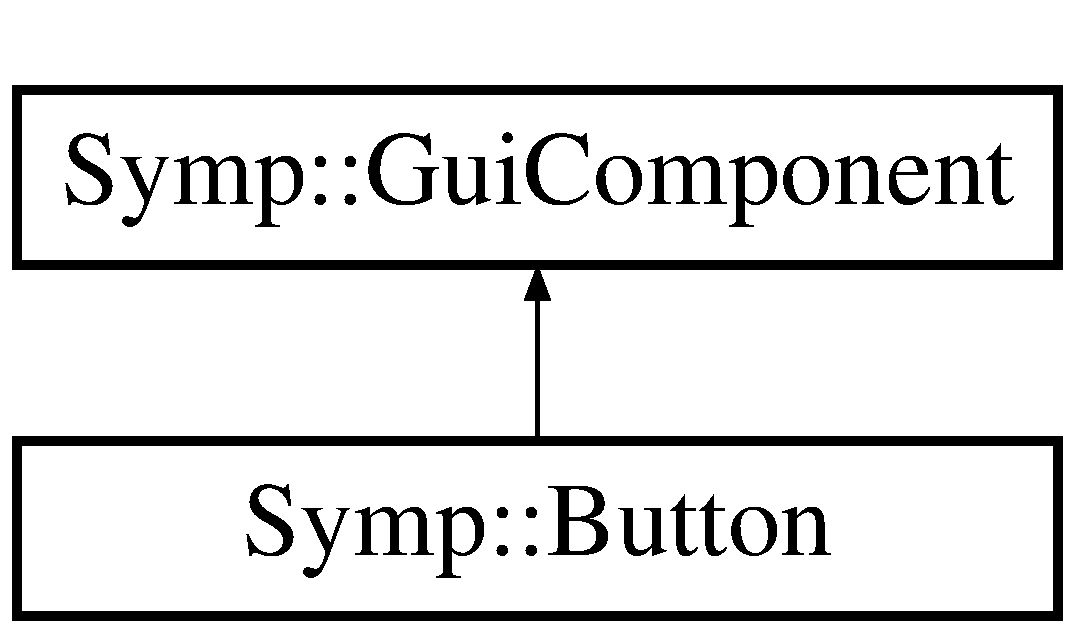
\includegraphics[height=2.000000cm]{class_symp_1_1_button}
\end{center}
\end{figure}
\subsection*{Public Member Functions}
\begin{DoxyCompactItemize}
\item 
\hyperlink{class_symp_1_1_button_a2de1604451d582a7c2e22344305212e5}{Button} (const char $\ast$file\-Path)
\begin{DoxyCompactList}\small\item\em \hyperlink{class_symp_1_1_button}{Button} class constructor inherits the \hyperlink{class_symp_1_1_gui_component}{Gui\-Component} class Responsible for the initialization of the only class private attribute. This constructor will associate a texture to its Indielib I\-N\-D\-\_\-\-Entity2d. See other constructor for drawing \hyperlink{class_symp_1_1_button_a2de1604451d582a7c2e22344305212e5}{Button} with text or color. \end{DoxyCompactList}\item 
\hyperlink{class_symp_1_1_button_a287f3fdf47224b349168a154534a8f30}{Button} (std\-::string text, \hyperlink{struct_symp_1_1_color}{Symp\-::\-Color} color=\hyperlink{struct_symp_1_1_color}{Color}(0, 0, 0), int i\-Weight=0)
\begin{DoxyCompactList}\small\item\em \hyperlink{class_symp_1_1_button}{Button} class constructor inherits the \hyperlink{class_symp_1_1_gui_component}{Gui\-Component} class Responsible for the initialization of the only class private attribute. This constructor will display a text on the \hyperlink{class_symp_1_1_button_a2de1604451d582a7c2e22344305212e5}{Button} and can draw a colored background or a colored border to the \hyperlink{class_symp_1_1_button_a2de1604451d582a7c2e22344305212e5}{Button}. The \#color parameter and the \#i\-Weight parameter have default values that creates a default \hyperlink{class_symp_1_1_button_a2de1604451d582a7c2e22344305212e5}{Button} with white background. {\bfseries Note} \-: why aren't they any position/size parameters for the creation of the \hyperlink{class_symp_1_1_button_a2de1604451d582a7c2e22344305212e5}{Button} ? Because, most of time, this constructor will be used with a \#\-Layout. The \#\-Layout will be responsible for the \hyperlink{class_symp_1_1_button_a2de1604451d582a7c2e22344305212e5}{Button} size and position. If this constructor is not used with a \#\-Layout, then the size and position attributes must be set manually following the \hyperlink{class_symp_1_1_gui_component_a22124675c2976983ac18374f81cc3fb3}{Gui\-Component} functions. \end{DoxyCompactList}\item 
\hyperlink{class_symp_1_1_button_ac9ef62333a52cb81e76dbda11d26ee32}{Button} (\hyperlink{struct_symp_1_1_color}{Symp\-::\-Color} color, float f\-Pos\-X, float f\-Pos\-Y, int f\-Width, int f\-Height)
\begin{DoxyCompactList}\small\item\em \hyperlink{class_symp_1_1_button}{Button} class constructor inherits the \hyperlink{class_symp_1_1_gui_component}{Gui\-Component} class Responsible for the initialization of the only class private attribute. This constructor only draw one type of \hyperlink{class_symp_1_1_button_a2de1604451d582a7c2e22344305212e5}{Button} \-: a filled one. For drawing a border instead of a background, please see other \hyperlink{class_symp_1_1_button_a2de1604451d582a7c2e22344305212e5}{Button} constructors. {\bfseries Note} \-: this function was meant to be used in a standalone \char`\"{}way\char`\"{}. If you use this constructor with a \#\-Layout, then prefer other constructor, because there will redondancy of size and position informations otherwise. \end{DoxyCompactList}\item 
\hyperlink{class_symp_1_1_button_a447d8e03240d9c19a421c392aff9cd5b}{$\sim$\-Button} ()
\item 
virtual void \hyperlink{class_symp_1_1_button_a5cec3a7ede8af0c059d6430f971b276b}{update} ()
\begin{DoxyCompactList}\small\item\em \hyperlink{class_symp_1_1_button}{Button} update fonction Refresh the display of the \hyperlink{class_symp_1_1_button_a2de1604451d582a7c2e22344305212e5}{Button}. \end{DoxyCompactList}\item 
void \hyperlink{class_symp_1_1_button_a926c42a1754990a32d4e9ed0f0ac17ff}{fill} (\hyperlink{struct_symp_1_1_color}{Symp\-::\-Color} color)
\begin{DoxyCompactList}\small\item\em fill \hyperlink{class_symp_1_1_button}{Button}'s background function \end{DoxyCompactList}\item 
void \hyperlink{class_symp_1_1_button_a44df5d198c51903edec0ed94ef494674}{set\-Text} (std\-::string text)
\begin{DoxyCompactList}\small\item\em set the \hyperlink{class_symp_1_1_button}{Button}'s text \end{DoxyCompactList}\item 
std\-::string \hyperlink{class_symp_1_1_button_ad468381ce32ed90c3b8c4bb5412fde34}{get\-Text} () const 
\item 
\hyperlink{class_symp_1_1_text}{Text} $\ast$ \hyperlink{class_symp_1_1_button_ab686da4fd7b76aebc4f674db8b368a52}{get\-Text\-Entity} () const 
\end{DoxyCompactItemize}
\subsection*{Additional Inherited Members}


\subsection{Detailed Description}
\hyperlink{class_symp_1_1_button}{Button} class. This class inherits the \hyperlink{class_symp_1_1_gui_component_a22124675c2976983ac18374f81cc3fb3}{Gui\-Component} class. A \hyperlink{class_symp_1_1_button_a2de1604451d582a7c2e22344305212e5}{Button} is a clickable and selectable component that can display text, or texture, or be customized with border or background. The simpliest way to use \hyperlink{class_symp_1_1_button_a2de1604451d582a7c2e22344305212e5}{Button} is with the \#\-Layout class, that handle the position and the size of the \hyperlink{class_symp_1_1_button_a2de1604451d582a7c2e22344305212e5}{Button}. The only paramters left are the color and the type of \hyperlink{class_symp_1_1_button_a2de1604451d582a7c2e22344305212e5}{Button} that will be rendered. 

\begin{DoxySeeAlso}{See Also}
\hyperlink{class_symp_1_1_menu_manager}{Menu\-Manager} 

\hyperlink{class_symp_1_1_button}{Button} 

\hyperlink{class_symp_1_1_gui_component}{Gui\-Component} 

\hyperlink{class_symp_1_1_layout}{Layout} 
\end{DoxySeeAlso}


Definition at line 21 of file Button.\-h.



\subsection{Constructor \& Destructor Documentation}
\hypertarget{class_symp_1_1_button_a2de1604451d582a7c2e22344305212e5}{\index{Symp\-::\-Button@{Symp\-::\-Button}!Button@{Button}}
\index{Button@{Button}!Symp::Button@{Symp\-::\-Button}}
\subsubsection[{Button}]{\setlength{\rightskip}{0pt plus 5cm}Symp\-::\-Button\-::\-Button (
\begin{DoxyParamCaption}
\item[{const char $\ast$}]{file\-Path}
\end{DoxyParamCaption}
)}}\label{class_symp_1_1_button_a2de1604451d582a7c2e22344305212e5}


\hyperlink{class_symp_1_1_button}{Button} class constructor inherits the \hyperlink{class_symp_1_1_gui_component}{Gui\-Component} class Responsible for the initialization of the only class private attribute. This constructor will associate a texture to its Indielib I\-N\-D\-\_\-\-Entity2d. See other constructor for drawing \hyperlink{class_symp_1_1_button_a2de1604451d582a7c2e22344305212e5}{Button} with text or color. 


\begin{DoxyParams}{Parameters}
{\em file\-Path} & is the path to the image file \\
\hline
\end{DoxyParams}
\begin{DoxySeeAlso}{See Also}
\hyperlink{class_symp_1_1_button}{Button} 

\hyperlink{class_symp_1_1_button_a447d8e03240d9c19a421c392aff9cd5b}{$\sim$\-Button()} 

\hyperlink{class_symp_1_1_gui_component}{Gui\-Component} 
\end{DoxySeeAlso}


Definition at line 15 of file Button.\-cpp.

\hypertarget{class_symp_1_1_button_a287f3fdf47224b349168a154534a8f30}{\index{Symp\-::\-Button@{Symp\-::\-Button}!Button@{Button}}
\index{Button@{Button}!Symp::Button@{Symp\-::\-Button}}
\subsubsection[{Button}]{\setlength{\rightskip}{0pt plus 5cm}Symp\-::\-Button\-::\-Button (
\begin{DoxyParamCaption}
\item[{std\-::string}]{text, }
\item[{{\bf Symp\-::\-Color}}]{color = {\ttfamily {\bf Color}(0,0,0)}, }
\item[{int}]{i\-Weight = {\ttfamily 0}}
\end{DoxyParamCaption}
)}}\label{class_symp_1_1_button_a287f3fdf47224b349168a154534a8f30}


\hyperlink{class_symp_1_1_button}{Button} class constructor inherits the \hyperlink{class_symp_1_1_gui_component}{Gui\-Component} class Responsible for the initialization of the only class private attribute. This constructor will display a text on the \hyperlink{class_symp_1_1_button_a2de1604451d582a7c2e22344305212e5}{Button} and can draw a colored background or a colored border to the \hyperlink{class_symp_1_1_button_a2de1604451d582a7c2e22344305212e5}{Button}. The \#color parameter and the \#i\-Weight parameter have default values that creates a default \hyperlink{class_symp_1_1_button_a2de1604451d582a7c2e22344305212e5}{Button} with white background. {\bfseries Note} \-: why aren't they any position/size parameters for the creation of the \hyperlink{class_symp_1_1_button_a2de1604451d582a7c2e22344305212e5}{Button} ? Because, most of time, this constructor will be used with a \#\-Layout. The \#\-Layout will be responsible for the \hyperlink{class_symp_1_1_button_a2de1604451d582a7c2e22344305212e5}{Button} size and position. If this constructor is not used with a \#\-Layout, then the size and position attributes must be set manually following the \hyperlink{class_symp_1_1_gui_component_a22124675c2976983ac18374f81cc3fb3}{Gui\-Component} functions. 


\begin{DoxyParams}{Parameters}
{\em text} & is the text that will be displayed by the \hyperlink{class_symp_1_1_button_a2de1604451d582a7c2e22344305212e5}{Button} \\
\hline
{\em color} & is the color that will fill the \hyperlink{class_symp_1_1_button_a2de1604451d582a7c2e22344305212e5}{Button} following the \#i\-Weight attributes \\
\hline
{\em i\-Weight} & decide wether the \hyperlink{class_symp_1_1_button_a2de1604451d582a7c2e22344305212e5}{Button} will have background (i\-Weight = 0) or border (i\-Weight != 0) \\
\hline
\end{DoxyParams}
\begin{DoxySeeAlso}{See Also}
\hyperlink{class_symp_1_1_button}{Button} 

\hyperlink{class_symp_1_1_button_a447d8e03240d9c19a421c392aff9cd5b}{$\sim$\-Button()} 

\hyperlink{struct_symp_1_1_color}{Color} 

\hyperlink{class_symp_1_1_layout}{Layout} 

\hyperlink{class_symp_1_1_gui_component}{Gui\-Component} 
\end{DoxySeeAlso}


Definition at line 49 of file Button.\-cpp.

\hypertarget{class_symp_1_1_button_ac9ef62333a52cb81e76dbda11d26ee32}{\index{Symp\-::\-Button@{Symp\-::\-Button}!Button@{Button}}
\index{Button@{Button}!Symp::Button@{Symp\-::\-Button}}
\subsubsection[{Button}]{\setlength{\rightskip}{0pt plus 5cm}Symp\-::\-Button\-::\-Button (
\begin{DoxyParamCaption}
\item[{{\bf Symp\-::\-Color}}]{color, }
\item[{float}]{i\-Pos\-X, }
\item[{float}]{i\-Pos\-Y, }
\item[{int}]{i\-Width, }
\item[{int}]{i\-Height}
\end{DoxyParamCaption}
)}}\label{class_symp_1_1_button_ac9ef62333a52cb81e76dbda11d26ee32}


\hyperlink{class_symp_1_1_button}{Button} class constructor inherits the \hyperlink{class_symp_1_1_gui_component}{Gui\-Component} class Responsible for the initialization of the only class private attribute. This constructor only draw one type of \hyperlink{class_symp_1_1_button_a2de1604451d582a7c2e22344305212e5}{Button} \-: a filled one. For drawing a border instead of a background, please see other \hyperlink{class_symp_1_1_button_a2de1604451d582a7c2e22344305212e5}{Button} constructors. {\bfseries Note} \-: this function was meant to be used in a standalone \char`\"{}way\char`\"{}. If you use this constructor with a \#\-Layout, then prefer other constructor, because there will redondancy of size and position informations otherwise. 


\begin{DoxyParams}{Parameters}
{\em color} & is the color that will fill the \hyperlink{class_symp_1_1_button_a2de1604451d582a7c2e22344305212e5}{Button} \\
\hline
{\em f\-Pos\-X} & is the x position of the up-\/left corner of the \hyperlink{class_symp_1_1_button_a2de1604451d582a7c2e22344305212e5}{Button} (why a float ? because Indielib needs it) \\
\hline
{\em f\-Pos\-Y} & is the y position of the up-\/left corner of the \hyperlink{class_symp_1_1_button_a2de1604451d582a7c2e22344305212e5}{Button} (why a float ? because Indielib needs it) \\
\hline
\end{DoxyParams}
\begin{DoxySeeAlso}{See Also}
\hyperlink{class_symp_1_1_button}{Button} 

\hyperlink{class_symp_1_1_button_a447d8e03240d9c19a421c392aff9cd5b}{$\sim$\-Button()} 

\hyperlink{struct_symp_1_1_color}{Color} 

\hyperlink{class_symp_1_1_gui_component}{Gui\-Component} 
\end{DoxySeeAlso}


Definition at line 79 of file Button.\-cpp.

\hypertarget{class_symp_1_1_button_a447d8e03240d9c19a421c392aff9cd5b}{\index{Symp\-::\-Button@{Symp\-::\-Button}!$\sim$\-Button@{$\sim$\-Button}}
\index{$\sim$\-Button@{$\sim$\-Button}!Symp::Button@{Symp\-::\-Button}}
\subsubsection[{$\sim$\-Button}]{\setlength{\rightskip}{0pt plus 5cm}Symp\-::\-Button\-::$\sim$\-Button (
\begin{DoxyParamCaption}
{}
\end{DoxyParamCaption}
)\hspace{0.3cm}{\ttfamily [inline]}}}\label{class_symp_1_1_button_a447d8e03240d9c19a421c392aff9cd5b}


Definition at line 26 of file Button.\-h.



\subsection{Member Function Documentation}
\hypertarget{class_symp_1_1_button_a926c42a1754990a32d4e9ed0f0ac17ff}{\index{Symp\-::\-Button@{Symp\-::\-Button}!fill@{fill}}
\index{fill@{fill}!Symp::Button@{Symp\-::\-Button}}
\subsubsection[{fill}]{\setlength{\rightskip}{0pt plus 5cm}void Symp\-::\-Button\-::fill (
\begin{DoxyParamCaption}
\item[{{\bf Symp\-::\-Color}}]{color}
\end{DoxyParamCaption}
)}}\label{class_symp_1_1_button_a926c42a1754990a32d4e9ed0f0ac17ff}


fill \hyperlink{class_symp_1_1_button}{Button}'s background function 

\begin{DoxySeeAlso}{See Also}
\hyperlink{class_symp_1_1_button}{Button} 

\hyperlink{class_symp_1_1_button_a447d8e03240d9c19a421c392aff9cd5b}{$\sim$\-Button()} 

\hyperlink{struct_symp_1_1_color}{Color} 

\hyperlink{class_symp_1_1_gui_component}{Gui\-Component} 
\end{DoxySeeAlso}


Definition at line 151 of file Button.\-cpp.

\hypertarget{class_symp_1_1_button_ad468381ce32ed90c3b8c4bb5412fde34}{\index{Symp\-::\-Button@{Symp\-::\-Button}!get\-Text@{get\-Text}}
\index{get\-Text@{get\-Text}!Symp::Button@{Symp\-::\-Button}}
\subsubsection[{get\-Text}]{\setlength{\rightskip}{0pt plus 5cm}std\-::string Symp\-::\-Button\-::get\-Text (
\begin{DoxyParamCaption}
{}
\end{DoxyParamCaption}
) const\hspace{0.3cm}{\ttfamily [inline]}}}\label{class_symp_1_1_button_ad468381ce32ed90c3b8c4bb5412fde34}


Definition at line 36 of file Button.\-h.

\hypertarget{class_symp_1_1_button_ab686da4fd7b76aebc4f674db8b368a52}{\index{Symp\-::\-Button@{Symp\-::\-Button}!get\-Text\-Entity@{get\-Text\-Entity}}
\index{get\-Text\-Entity@{get\-Text\-Entity}!Symp::Button@{Symp\-::\-Button}}
\subsubsection[{get\-Text\-Entity}]{\setlength{\rightskip}{0pt plus 5cm}{\bf Text}$\ast$ Symp\-::\-Button\-::get\-Text\-Entity (
\begin{DoxyParamCaption}
{}
\end{DoxyParamCaption}
) const\hspace{0.3cm}{\ttfamily [inline]}}}\label{class_symp_1_1_button_ab686da4fd7b76aebc4f674db8b368a52}


Definition at line 37 of file Button.\-h.

\hypertarget{class_symp_1_1_button_a44df5d198c51903edec0ed94ef494674}{\index{Symp\-::\-Button@{Symp\-::\-Button}!set\-Text@{set\-Text}}
\index{set\-Text@{set\-Text}!Symp::Button@{Symp\-::\-Button}}
\subsubsection[{set\-Text}]{\setlength{\rightskip}{0pt plus 5cm}void Symp\-::\-Button\-::set\-Text (
\begin{DoxyParamCaption}
\item[{std\-::string}]{text}
\end{DoxyParamCaption}
)}}\label{class_symp_1_1_button_a44df5d198c51903edec0ed94ef494674}


set the \hyperlink{class_symp_1_1_button}{Button}'s text 

\begin{DoxyRefDesc}{Bug}
\item[\hyperlink{bug__bug000001}{Bug}]/!\textbackslash{} N\-O\-T W\-O\-R\-K\-I\-N\-G Y\-E\-T /!\textbackslash{} \end{DoxyRefDesc}
\begin{DoxySeeAlso}{See Also}
\hyperlink{class_symp_1_1_button}{Button} 

\hyperlink{class_symp_1_1_button_a447d8e03240d9c19a421c392aff9cd5b}{$\sim$\-Button()} 

\hyperlink{class_symp_1_1_gui_component}{Gui\-Component} 
\end{DoxySeeAlso}


Definition at line 163 of file Button.\-cpp.

\hypertarget{class_symp_1_1_button_a5cec3a7ede8af0c059d6430f971b276b}{\index{Symp\-::\-Button@{Symp\-::\-Button}!update@{update}}
\index{update@{update}!Symp::Button@{Symp\-::\-Button}}
\subsubsection[{update}]{\setlength{\rightskip}{0pt plus 5cm}void Symp\-::\-Button\-::update (
\begin{DoxyParamCaption}
{}
\end{DoxyParamCaption}
)\hspace{0.3cm}{\ttfamily [virtual]}}}\label{class_symp_1_1_button_a5cec3a7ede8af0c059d6430f971b276b}


\hyperlink{class_symp_1_1_button}{Button} update fonction Refresh the display of the \hyperlink{class_symp_1_1_button_a2de1604451d582a7c2e22344305212e5}{Button}. 

\begin{DoxySeeAlso}{See Also}
\hyperlink{class_symp_1_1_button}{Button} 

\hyperlink{class_symp_1_1_button_a447d8e03240d9c19a421c392aff9cd5b}{$\sim$\-Button()} 

\hyperlink{class_symp_1_1_gui_component}{Gui\-Component} 
\end{DoxySeeAlso}


Implements \hyperlink{class_symp_1_1_gui_component_add73e07ea0a3c9c1c90640e783a3b5de}{Symp\-::\-Gui\-Component}.



Definition at line 104 of file Button.\-cpp.



The documentation for this class was generated from the following files\-:\begin{DoxyCompactItemize}
\item 
/home/cecilia/\-Documents/\-Symptogen/src/menu/\hyperlink{_button_8h}{Button.\-h}\item 
/home/cecilia/\-Documents/\-Symptogen/src/menu/\hyperlink{_button_8cpp}{Button.\-cpp}\end{DoxyCompactItemize}

\hypertarget{class_symp_1_1_camera}{\section{Symp\-:\-:Camera Class Reference}
\label{class_symp_1_1_camera}\index{Symp\-::\-Camera@{Symp\-::\-Camera}}
}


{\ttfamily \#include $<$Camera.\-h$>$}

\subsection*{Public Member Functions}
\begin{DoxyCompactItemize}
\item 
\hyperlink{class_symp_1_1_camera_af329ce691bb2cd89448962d6972e2398}{Camera} ()
\item 
\hyperlink{class_symp_1_1_camera_ada55171c7ddcea56cfb6317a1d1ce753}{$\sim$\-Camera} ()
\item 
void \hyperlink{class_symp_1_1_camera_adfdd7f8e25d66f4d8fd4b59b2b2e074a}{reset} (float dino\-Pos\-X, float dino\-Pos\-Y)
\item 
void \hyperlink{class_symp_1_1_camera_aa2e99343c4f8c6536f0adcdef90e6334}{set\-Position} (float pos\-X, float pos\-Y)
\item 
void \hyperlink{class_symp_1_1_camera_a45cdeda6f35ac95266c051b5776a3f8b}{set\-Zoom} (float zoom)
\item 
void \hyperlink{class_symp_1_1_camera_a7b5eebebf3ad1faeb78007ac21a4d004}{set\-Angle} (float angle)
\item 
I\-N\-D\-\_\-\-Camera2d $\ast$ \hyperlink{class_symp_1_1_camera_a22de9a53595e14bcd8d0f9f0e94c32f5}{get\-I\-N\-D\-\_\-\-Camera2d} ()
\end{DoxyCompactItemize}


\subsection{Detailed Description}
Facade of I\-N\-D\-\_\-\-Camera2d. 

Definition at line 13 of file Camera.\-h.



\subsection{Constructor \& Destructor Documentation}
\hypertarget{class_symp_1_1_camera_af329ce691bb2cd89448962d6972e2398}{\index{Symp\-::\-Camera@{Symp\-::\-Camera}!Camera@{Camera}}
\index{Camera@{Camera}!Symp::Camera@{Symp\-::\-Camera}}
\subsubsection[{Camera}]{\setlength{\rightskip}{0pt plus 5cm}Symp\-::\-Camera\-::\-Camera (
\begin{DoxyParamCaption}
{}
\end{DoxyParamCaption}
)}}\label{class_symp_1_1_camera_af329ce691bb2cd89448962d6972e2398}


Definition at line 5 of file Camera.\-cpp.

\hypertarget{class_symp_1_1_camera_ada55171c7ddcea56cfb6317a1d1ce753}{\index{Symp\-::\-Camera@{Symp\-::\-Camera}!$\sim$\-Camera@{$\sim$\-Camera}}
\index{$\sim$\-Camera@{$\sim$\-Camera}!Symp::Camera@{Symp\-::\-Camera}}
\subsubsection[{$\sim$\-Camera}]{\setlength{\rightskip}{0pt plus 5cm}Symp\-::\-Camera\-::$\sim$\-Camera (
\begin{DoxyParamCaption}
{}
\end{DoxyParamCaption}
)}}\label{class_symp_1_1_camera_ada55171c7ddcea56cfb6317a1d1ce753}


Definition at line 9 of file Camera.\-cpp.



\subsection{Member Function Documentation}
\hypertarget{class_symp_1_1_camera_a22de9a53595e14bcd8d0f9f0e94c32f5}{\index{Symp\-::\-Camera@{Symp\-::\-Camera}!get\-I\-N\-D\-\_\-\-Camera2d@{get\-I\-N\-D\-\_\-\-Camera2d}}
\index{get\-I\-N\-D\-\_\-\-Camera2d@{get\-I\-N\-D\-\_\-\-Camera2d}!Symp::Camera@{Symp\-::\-Camera}}
\subsubsection[{get\-I\-N\-D\-\_\-\-Camera2d}]{\setlength{\rightskip}{0pt plus 5cm}I\-N\-D\-\_\-\-Camera2d$\ast$ Symp\-::\-Camera\-::get\-I\-N\-D\-\_\-\-Camera2d (
\begin{DoxyParamCaption}
{}
\end{DoxyParamCaption}
)\hspace{0.3cm}{\ttfamily [inline]}}}\label{class_symp_1_1_camera_a22de9a53595e14bcd8d0f9f0e94c32f5}


Definition at line 24 of file Camera.\-h.

\hypertarget{class_symp_1_1_camera_adfdd7f8e25d66f4d8fd4b59b2b2e074a}{\index{Symp\-::\-Camera@{Symp\-::\-Camera}!reset@{reset}}
\index{reset@{reset}!Symp::Camera@{Symp\-::\-Camera}}
\subsubsection[{reset}]{\setlength{\rightskip}{0pt plus 5cm}void Symp\-::\-Camera\-::reset (
\begin{DoxyParamCaption}
\item[{float}]{dino\-Pos\-X, }
\item[{float}]{dino\-Pos\-Y}
\end{DoxyParamCaption}
)}}\label{class_symp_1_1_camera_adfdd7f8e25d66f4d8fd4b59b2b2e074a}


Definition at line 13 of file Camera.\-cpp.

\hypertarget{class_symp_1_1_camera_a7b5eebebf3ad1faeb78007ac21a4d004}{\index{Symp\-::\-Camera@{Symp\-::\-Camera}!set\-Angle@{set\-Angle}}
\index{set\-Angle@{set\-Angle}!Symp::Camera@{Symp\-::\-Camera}}
\subsubsection[{set\-Angle}]{\setlength{\rightskip}{0pt plus 5cm}void Symp\-::\-Camera\-::set\-Angle (
\begin{DoxyParamCaption}
\item[{float}]{angle}
\end{DoxyParamCaption}
)}}\label{class_symp_1_1_camera_a7b5eebebf3ad1faeb78007ac21a4d004}


Definition at line 25 of file Camera.\-cpp.

\hypertarget{class_symp_1_1_camera_aa2e99343c4f8c6536f0adcdef90e6334}{\index{Symp\-::\-Camera@{Symp\-::\-Camera}!set\-Position@{set\-Position}}
\index{set\-Position@{set\-Position}!Symp::Camera@{Symp\-::\-Camera}}
\subsubsection[{set\-Position}]{\setlength{\rightskip}{0pt plus 5cm}void Symp\-::\-Camera\-::set\-Position (
\begin{DoxyParamCaption}
\item[{float}]{pos\-X, }
\item[{float}]{pos\-Y}
\end{DoxyParamCaption}
)}}\label{class_symp_1_1_camera_aa2e99343c4f8c6536f0adcdef90e6334}


Definition at line 17 of file Camera.\-cpp.

\hypertarget{class_symp_1_1_camera_a45cdeda6f35ac95266c051b5776a3f8b}{\index{Symp\-::\-Camera@{Symp\-::\-Camera}!set\-Zoom@{set\-Zoom}}
\index{set\-Zoom@{set\-Zoom}!Symp::Camera@{Symp\-::\-Camera}}
\subsubsection[{set\-Zoom}]{\setlength{\rightskip}{0pt plus 5cm}void Symp\-::\-Camera\-::set\-Zoom (
\begin{DoxyParamCaption}
\item[{float}]{zoom}
\end{DoxyParamCaption}
)}}\label{class_symp_1_1_camera_a45cdeda6f35ac95266c051b5776a3f8b}


Definition at line 21 of file Camera.\-cpp.



The documentation for this class was generated from the following files\-:\begin{DoxyCompactItemize}
\item 
/home/cecilia/\-Documents/\-Symptogen/src/render/\hyperlink{_camera_8h}{Camera.\-h}\item 
/home/cecilia/\-Documents/\-Symptogen/src/render/\hyperlink{_camera_8cpp}{Camera.\-cpp}\end{DoxyCompactItemize}

\hypertarget{class_symp_1_1_choose_your_level_menu}{\section{Symp\-:\-:Choose\-Your\-Level\-Menu Class Reference}
\label{class_symp_1_1_choose_your_level_menu}\index{Symp\-::\-Choose\-Your\-Level\-Menu@{Symp\-::\-Choose\-Your\-Level\-Menu}}
}


{\ttfamily \#include $<$Choose\-Your\-Level\-Menu.\-h$>$}

Inheritance diagram for Symp\-:\-:Choose\-Your\-Level\-Menu\-:\begin{figure}[H]
\begin{center}
\leavevmode
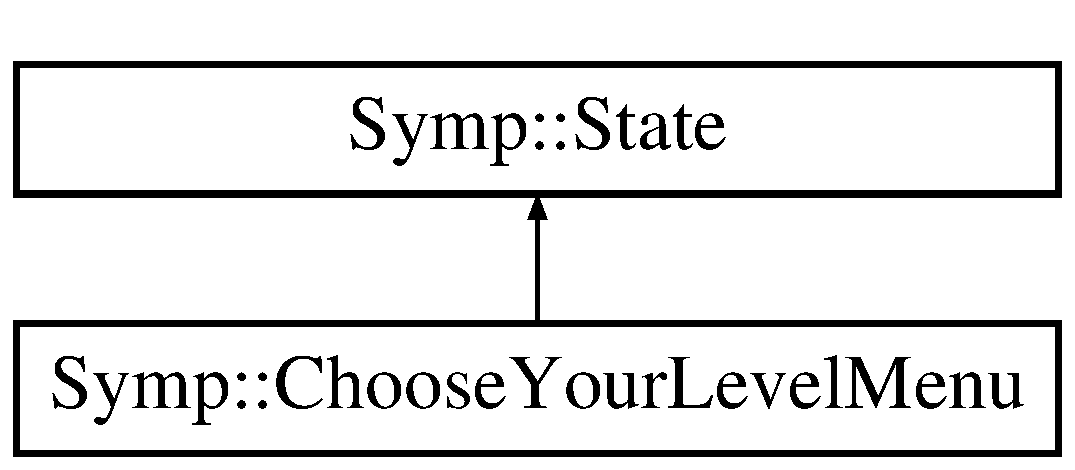
\includegraphics[height=2.000000cm]{class_symp_1_1_choose_your_level_menu}
\end{center}
\end{figure}
\subsection*{Public Member Functions}
\begin{DoxyCompactItemize}
\item 
\hyperlink{class_symp_1_1_choose_your_level_menu_a98ee0f524c03693196a26a733cc49c3b}{Choose\-Your\-Level\-Menu} (\hyperlink{class_symp_1_1_player}{Player} $\ast$p\-Player)
\begin{DoxyCompactList}\small\item\em Choose\-Your\-Level constructor Responsible for the initialization of the private attributes of the \hyperlink{class_symp_1_1_choose_your_level_menu_a98ee0f524c03693196a26a733cc49c3b}{Choose\-Your\-Level\-Menu} class. This function is not responsible for drawing the graphical elements that compose the menu, the \hyperlink{class_symp_1_1_choose_your_level_menu_a18c2d2aec31b070ecdd5ec8d2c8b4cbf}{init()} function is. \end{DoxyCompactList}\item 
\hyperlink{class_symp_1_1_choose_your_level_menu_af744c7af3ef5a5b3011b441539c3743f}{$\sim$\-Choose\-Your\-Level\-Menu} ()
\item 
virtual void \hyperlink{class_symp_1_1_choose_your_level_menu_a18c2d2aec31b070ecdd5ec8d2c8b4cbf}{init} ()
\begin{DoxyCompactList}\small\item\em Choose\-Your\-Level elements initialization The elements that compose the menu are created in this function. \end{DoxyCompactList}\item 
virtual void \hyperlink{class_symp_1_1_choose_your_level_menu_a8c3ad10284b68e12df75ff980a7fc657}{handle\-Mouse\-Clic} (int mouse\-X, int mouse\-Y)
\begin{DoxyCompactList}\small\item\em Handle mouse clic events. \end{DoxyCompactList}\item 
virtual void \hyperlink{class_symp_1_1_choose_your_level_menu_a2a66e7d44ceca790b987eca33fa478ff}{key\-Down\-Pressed} ()
\begin{DoxyCompactList}\small\item\em Handle key down event. \end{DoxyCompactList}\item 
virtual void \hyperlink{class_symp_1_1_choose_your_level_menu_a59974b0d10b806ed646569b4b658d68f}{key\-Up\-Pressed} ()
\begin{DoxyCompactList}\small\item\em Handle key up event. \end{DoxyCompactList}\item 
std\-::string \hyperlink{class_symp_1_1_choose_your_level_menu_a2702263ebb7be3e86a62dadfc0f098cd}{get\-Level\-Name} (int level)
\item 
\hyperlink{class_symp_1_1_player}{Player} $\ast$ \hyperlink{class_symp_1_1_choose_your_level_menu_a4b0cc48f521c2f315e2b5995a6a0b3f8}{get\-Player} () const 
\end{DoxyCompactItemize}


\subsection{Detailed Description}
the \hyperlink{class_symp_1_1_state_ad44d90b6e1b68eb021ceaa0cb98141a4}{State} interface for implementing the \hyperlink{class_symp_1_1_state}{State} Machine Pattern This Menu show the personal panel of a player. The player can see its current level, and can replay any level he already finished. From that menu, the user can go back to \#\-Manage\-Games\-Menu or launch a game by clicking on a level. \begin{DoxySeeAlso}{See Also}
\hyperlink{class_symp_1_1_state}{State} 

\hyperlink{class_symp_1_1_game_manager}{Game\-Manager} 

\hyperlink{class_symp_1_1_manage_games_menu}{Manage\-Games\-Menu} 

\hyperlink{class_symp_1_1_menu_manager}{Menu\-Manager} 
\end{DoxySeeAlso}


Definition at line 20 of file Choose\-Your\-Level\-Menu.\-h.



\subsection{Constructor \& Destructor Documentation}
\hypertarget{class_symp_1_1_choose_your_level_menu_a98ee0f524c03693196a26a733cc49c3b}{\index{Symp\-::\-Choose\-Your\-Level\-Menu@{Symp\-::\-Choose\-Your\-Level\-Menu}!Choose\-Your\-Level\-Menu@{Choose\-Your\-Level\-Menu}}
\index{Choose\-Your\-Level\-Menu@{Choose\-Your\-Level\-Menu}!Symp::ChooseYourLevelMenu@{Symp\-::\-Choose\-Your\-Level\-Menu}}
\subsubsection[{Choose\-Your\-Level\-Menu}]{\setlength{\rightskip}{0pt plus 5cm}Symp\-::\-Choose\-Your\-Level\-Menu\-::\-Choose\-Your\-Level\-Menu (
\begin{DoxyParamCaption}
\item[{{\bf Player} $\ast$}]{p\-Player}
\end{DoxyParamCaption}
)}}\label{class_symp_1_1_choose_your_level_menu_a98ee0f524c03693196a26a733cc49c3b}


Choose\-Your\-Level constructor Responsible for the initialization of the private attributes of the \hyperlink{class_symp_1_1_choose_your_level_menu_a98ee0f524c03693196a26a733cc49c3b}{Choose\-Your\-Level\-Menu} class. This function is not responsible for drawing the graphical elements that compose the menu, the \hyperlink{class_symp_1_1_choose_your_level_menu_a18c2d2aec31b070ecdd5ec8d2c8b4cbf}{init()} function is. 


\begin{DoxyParams}{Parameters}
{\em p\-Player} & the reference to the \#\-Player \\
\hline
{\em p\-Menu\-Manager} & the reference to the \#\-Menu\-Manager \\
\hline
\end{DoxyParams}
\begin{DoxySeeAlso}{See Also}
\hyperlink{class_symp_1_1_player}{Player} 

\hyperlink{class_symp_1_1_menu_manager}{Menu\-Manager} 

\hyperlink{class_symp_1_1_state}{State} 

\hyperlink{class_symp_1_1_choose_your_level_menu_a18c2d2aec31b070ecdd5ec8d2c8b4cbf}{init()} 

\hyperlink{class_symp_1_1_choose_your_level_menu_af744c7af3ef5a5b3011b441539c3743f}{$\sim$\-Choose\-Your\-Level\-Menu()} 
\end{DoxySeeAlso}


Definition at line 23 of file Choose\-Your\-Level\-Menu.\-cpp.

\hypertarget{class_symp_1_1_choose_your_level_menu_af744c7af3ef5a5b3011b441539c3743f}{\index{Symp\-::\-Choose\-Your\-Level\-Menu@{Symp\-::\-Choose\-Your\-Level\-Menu}!$\sim$\-Choose\-Your\-Level\-Menu@{$\sim$\-Choose\-Your\-Level\-Menu}}
\index{$\sim$\-Choose\-Your\-Level\-Menu@{$\sim$\-Choose\-Your\-Level\-Menu}!Symp::ChooseYourLevelMenu@{Symp\-::\-Choose\-Your\-Level\-Menu}}
\subsubsection[{$\sim$\-Choose\-Your\-Level\-Menu}]{\setlength{\rightskip}{0pt plus 5cm}Symp\-::\-Choose\-Your\-Level\-Menu\-::$\sim$\-Choose\-Your\-Level\-Menu (
\begin{DoxyParamCaption}
{}
\end{DoxyParamCaption}
)\hspace{0.3cm}{\ttfamily [inline]}}}\label{class_symp_1_1_choose_your_level_menu_af744c7af3ef5a5b3011b441539c3743f}


Definition at line 23 of file Choose\-Your\-Level\-Menu.\-h.



\subsection{Member Function Documentation}
\hypertarget{class_symp_1_1_choose_your_level_menu_a2702263ebb7be3e86a62dadfc0f098cd}{\index{Symp\-::\-Choose\-Your\-Level\-Menu@{Symp\-::\-Choose\-Your\-Level\-Menu}!get\-Level\-Name@{get\-Level\-Name}}
\index{get\-Level\-Name@{get\-Level\-Name}!Symp::ChooseYourLevelMenu@{Symp\-::\-Choose\-Your\-Level\-Menu}}
\subsubsection[{get\-Level\-Name}]{\setlength{\rightskip}{0pt plus 5cm}std\-::string Symp\-::\-Choose\-Your\-Level\-Menu\-::get\-Level\-Name (
\begin{DoxyParamCaption}
\item[{int}]{level}
\end{DoxyParamCaption}
)}}\label{class_symp_1_1_choose_your_level_menu_a2702263ebb7be3e86a62dadfc0f098cd}


Definition at line 200 of file Choose\-Your\-Level\-Menu.\-cpp.

\hypertarget{class_symp_1_1_choose_your_level_menu_a4b0cc48f521c2f315e2b5995a6a0b3f8}{\index{Symp\-::\-Choose\-Your\-Level\-Menu@{Symp\-::\-Choose\-Your\-Level\-Menu}!get\-Player@{get\-Player}}
\index{get\-Player@{get\-Player}!Symp::ChooseYourLevelMenu@{Symp\-::\-Choose\-Your\-Level\-Menu}}
\subsubsection[{get\-Player}]{\setlength{\rightskip}{0pt plus 5cm}{\bf Player}$\ast$ Symp\-::\-Choose\-Your\-Level\-Menu\-::get\-Player (
\begin{DoxyParamCaption}
{}
\end{DoxyParamCaption}
) const\hspace{0.3cm}{\ttfamily [inline]}}}\label{class_symp_1_1_choose_your_level_menu_a4b0cc48f521c2f315e2b5995a6a0b3f8}


Definition at line 33 of file Choose\-Your\-Level\-Menu.\-h.

\hypertarget{class_symp_1_1_choose_your_level_menu_a8c3ad10284b68e12df75ff980a7fc657}{\index{Symp\-::\-Choose\-Your\-Level\-Menu@{Symp\-::\-Choose\-Your\-Level\-Menu}!handle\-Mouse\-Clic@{handle\-Mouse\-Clic}}
\index{handle\-Mouse\-Clic@{handle\-Mouse\-Clic}!Symp::ChooseYourLevelMenu@{Symp\-::\-Choose\-Your\-Level\-Menu}}
\subsubsection[{handle\-Mouse\-Clic}]{\setlength{\rightskip}{0pt plus 5cm}void Symp\-::\-Choose\-Your\-Level\-Menu\-::handle\-Mouse\-Clic (
\begin{DoxyParamCaption}
\item[{int}]{mouse\-X, }
\item[{int}]{mouse\-Y}
\end{DoxyParamCaption}
)\hspace{0.3cm}{\ttfamily [virtual]}}}\label{class_symp_1_1_choose_your_level_menu_a8c3ad10284b68e12df75ff980a7fc657}


Handle mouse clic events. 


\begin{DoxyParams}{Parameters}
{\em mouse\-X} & the x coordinate of the mouse position \\
\hline
{\em mouse\-Y} & the y coordinate of the mouse position \\
\hline
\end{DoxyParams}
\begin{DoxySeeAlso}{See Also}
\hyperlink{class_symp_1_1_menu_manager}{Menu\-Manager} 

\hyperlink{class_symp_1_1_state}{State} 

\hyperlink{class_symp_1_1_input_manager}{Input\-Manager} 

\hyperlink{class_symp_1_1_choose_your_level_menu_a18c2d2aec31b070ecdd5ec8d2c8b4cbf}{init()} 
\end{DoxySeeAlso}


Implements \hyperlink{class_symp_1_1_state_a23e468a10d9be4c79d17e22d1d5ef478}{Symp\-::\-State}.



Definition at line 180 of file Choose\-Your\-Level\-Menu.\-cpp.

\hypertarget{class_symp_1_1_choose_your_level_menu_a18c2d2aec31b070ecdd5ec8d2c8b4cbf}{\index{Symp\-::\-Choose\-Your\-Level\-Menu@{Symp\-::\-Choose\-Your\-Level\-Menu}!init@{init}}
\index{init@{init}!Symp::ChooseYourLevelMenu@{Symp\-::\-Choose\-Your\-Level\-Menu}}
\subsubsection[{init}]{\setlength{\rightskip}{0pt plus 5cm}void Symp\-::\-Choose\-Your\-Level\-Menu\-::init (
\begin{DoxyParamCaption}
{}
\end{DoxyParamCaption}
)\hspace{0.3cm}{\ttfamily [virtual]}}}\label{class_symp_1_1_choose_your_level_menu_a18c2d2aec31b070ecdd5ec8d2c8b4cbf}


Choose\-Your\-Level elements initialization The elements that compose the menu are created in this function. 

\begin{DoxySeeAlso}{See Also}
\hyperlink{class_symp_1_1_player}{Player} 

\hyperlink{class_symp_1_1_menu_manager}{Menu\-Manager} 

\hyperlink{class_symp_1_1_state}{State} 

end() 

\hyperlink{class_symp_1_1_choose_your_level_menu_a98ee0f524c03693196a26a733cc49c3b}{Choose\-Your\-Level\-Menu()} 
\end{DoxySeeAlso}


Implements \hyperlink{class_symp_1_1_state_a2c1c597b1235128a356c7529c42fdec3}{Symp\-::\-State}.



Definition at line 36 of file Choose\-Your\-Level\-Menu.\-cpp.

\hypertarget{class_symp_1_1_choose_your_level_menu_a2a66e7d44ceca790b987eca33fa478ff}{\index{Symp\-::\-Choose\-Your\-Level\-Menu@{Symp\-::\-Choose\-Your\-Level\-Menu}!key\-Down\-Pressed@{key\-Down\-Pressed}}
\index{key\-Down\-Pressed@{key\-Down\-Pressed}!Symp::ChooseYourLevelMenu@{Symp\-::\-Choose\-Your\-Level\-Menu}}
\subsubsection[{key\-Down\-Pressed}]{\setlength{\rightskip}{0pt plus 5cm}void Symp\-::\-Choose\-Your\-Level\-Menu\-::key\-Down\-Pressed (
\begin{DoxyParamCaption}
{}
\end{DoxyParamCaption}
)\hspace{0.3cm}{\ttfamily [virtual]}}}\label{class_symp_1_1_choose_your_level_menu_a2a66e7d44ceca790b987eca33fa478ff}


Handle key down event. 

\begin{DoxySeeAlso}{See Also}
\hyperlink{class_symp_1_1_menu_manager}{Menu\-Manager} 

\hyperlink{class_symp_1_1_state}{State} 

\hyperlink{class_symp_1_1_input_manager}{Input\-Manager} 

\hyperlink{class_symp_1_1_choose_your_level_menu_a18c2d2aec31b070ecdd5ec8d2c8b4cbf}{init()} 
\end{DoxySeeAlso}


Implements \hyperlink{class_symp_1_1_state_ac9ff920d185cdc17c9bc3ac63b40c62d}{Symp\-::\-State}.



Definition at line 227 of file Choose\-Your\-Level\-Menu.\-cpp.

\hypertarget{class_symp_1_1_choose_your_level_menu_a59974b0d10b806ed646569b4b658d68f}{\index{Symp\-::\-Choose\-Your\-Level\-Menu@{Symp\-::\-Choose\-Your\-Level\-Menu}!key\-Up\-Pressed@{key\-Up\-Pressed}}
\index{key\-Up\-Pressed@{key\-Up\-Pressed}!Symp::ChooseYourLevelMenu@{Symp\-::\-Choose\-Your\-Level\-Menu}}
\subsubsection[{key\-Up\-Pressed}]{\setlength{\rightskip}{0pt plus 5cm}void Symp\-::\-Choose\-Your\-Level\-Menu\-::key\-Up\-Pressed (
\begin{DoxyParamCaption}
{}
\end{DoxyParamCaption}
)\hspace{0.3cm}{\ttfamily [virtual]}}}\label{class_symp_1_1_choose_your_level_menu_a59974b0d10b806ed646569b4b658d68f}


Handle key up event. 

\begin{DoxySeeAlso}{See Also}
\hyperlink{class_symp_1_1_menu_manager}{Menu\-Manager} 

\hyperlink{class_symp_1_1_state}{State} 

\hyperlink{class_symp_1_1_input_manager}{Input\-Manager} 

\hyperlink{class_symp_1_1_choose_your_level_menu_a18c2d2aec31b070ecdd5ec8d2c8b4cbf}{init()} 
\end{DoxySeeAlso}


Implements \hyperlink{class_symp_1_1_state_a67d0fc2a02808bbcfdb06935c3be404f}{Symp\-::\-State}.



Definition at line 238 of file Choose\-Your\-Level\-Menu.\-cpp.



The documentation for this class was generated from the following files\-:\begin{DoxyCompactItemize}
\item 
/home/cecilia/\-Documents/\-Symptogen/src/menu/\hyperlink{_choose_your_level_menu_8h}{Choose\-Your\-Level\-Menu.\-h}\item 
/home/cecilia/\-Documents/\-Symptogen/src/menu/\hyperlink{_choose_your_level_menu_8cpp}{Choose\-Your\-Level\-Menu.\-cpp}\end{DoxyCompactItemize}

\hypertarget{struct_symp_1_1_color}{\section{Symp\-:\-:Color Class Reference}
\label{struct_symp_1_1_color}\index{Symp\-::\-Color@{Symp\-::\-Color}}
}


{\ttfamily \#include $<$Gui\-Component.\-h$>$}

\subsection*{Public Member Functions}
\begin{DoxyCompactItemize}
\item 
\hyperlink{struct_symp_1_1_color_a182d56f6f2b8ad205d686845504d755e}{Color} (unsigned int r\-Value, unsigned int g\-Value, unsigned int b\-Value, unsigned int a\-Value=255)
\begin{DoxyCompactList}\small\item\em \hyperlink{struct_symp_1_1_color}{Color} struct constructor. Responsible for the initialization of private attributes of the \hyperlink{struct_symp_1_1_color}{Color} class. \end{DoxyCompactList}\end{DoxyCompactItemize}
\subsection*{Public Attributes}
\begin{DoxyCompactItemize}
\item 
unsigned int \hyperlink{struct_symp_1_1_color_aa793f972ed87529d8b841d601a575faa}{r}
\item 
unsigned int \hyperlink{struct_symp_1_1_color_a9647c7f07beac0f0851609a3ba2db21c}{g}
\item 
unsigned int \hyperlink{struct_symp_1_1_color_a71b5f200ef4f3b72ab507bc9cd41e8cc}{b}
\item 
unsigned int \hyperlink{struct_symp_1_1_color_af948ec8fb21c5e8faaa2061fe4122953}{a}
\end{DoxyCompactItemize}
\subsection*{Static Public Attributes}
\begin{DoxyCompactItemize}
\item 
static const \hyperlink{struct_symp_1_1_color}{Color} \hyperlink{struct_symp_1_1_color_a8585c0abfc6ae44172bcbc7e1bbc54bf}{B\-L\-U\-E} = \hyperlink{struct_symp_1_1_color}{Color}(0, 0, 255)
\item 
static const \hyperlink{struct_symp_1_1_color}{Color} \hyperlink{struct_symp_1_1_color_ade2892a390cd549444d84da71164e67d}{R\-E\-D} = \hyperlink{struct_symp_1_1_color}{Color}(255, 0, 0)
\item 
static const \hyperlink{struct_symp_1_1_color}{Color} \hyperlink{struct_symp_1_1_color_af8e6c9ee96133ee641e9b48a1eae788b}{G\-R\-E\-E\-N} = \hyperlink{struct_symp_1_1_color}{Color}(0, 255, 0)
\item 
static const \hyperlink{struct_symp_1_1_color}{Color} \hyperlink{struct_symp_1_1_color_a8a38032122222aad1e32aae688d27a23}{B\-L\-A\-C\-K} = \hyperlink{struct_symp_1_1_color}{Color}(0, 0, 0)
\item 
static const \hyperlink{struct_symp_1_1_color}{Color} \hyperlink{struct_symp_1_1_color_ae40a5f0273adf627d6ff49fa0e5669d8}{G\-R\-E\-Y} = \hyperlink{struct_symp_1_1_color}{Color}(180, 180, 180)
\item 
static const \hyperlink{struct_symp_1_1_color}{Color} \hyperlink{struct_symp_1_1_color_a501e4889d9f64917b89b762de9f2e200}{W\-H\-I\-T\-E} = \hyperlink{struct_symp_1_1_color}{Color}(255, 255, 255)
\item 
static const \hyperlink{struct_symp_1_1_color}{Color} \hyperlink{struct_symp_1_1_color_aaeb71736387c37c7df2b0ea9b0cc6417}{B\-L\-U\-E\-D\-I\-N\-O} = \hyperlink{struct_symp_1_1_color}{Color}(121, 206, 206)
\item 
static const \hyperlink{struct_symp_1_1_color}{Color} \hyperlink{struct_symp_1_1_color_a53e70f54d10aa2f707e2f0f97b33fde7}{Y\-E\-L\-L\-O\-W\-D\-I\-N\-O} = \hyperlink{struct_symp_1_1_color}{Color}(253, 254, 24)
\end{DoxyCompactItemize}


\subsection{Detailed Description}
The \hyperlink{struct_symp_1_1_color}{Color} struct presents convenient fields for the definition of a color, following the classic R\-G\-B\-A convention. Mostly used for defining background and border colors in \hyperlink{class_symp_1_1_layout}{Layout} and \hyperlink{class_symp_1_1_button}{Button} class. \begin{DoxySeeAlso}{See Also}
\hyperlink{class_symp_1_1_gui_component}{Gui\-Component} 

\hyperlink{class_symp_1_1_layout}{Layout} 

\hyperlink{class_symp_1_1_button}{Button} 
\end{DoxySeeAlso}


Definition at line 24 of file Gui\-Component.\-h.



\subsection{Constructor \& Destructor Documentation}
\hypertarget{struct_symp_1_1_color_a182d56f6f2b8ad205d686845504d755e}{\index{Symp\-::\-Color@{Symp\-::\-Color}!Color@{Color}}
\index{Color@{Color}!Symp::Color@{Symp\-::\-Color}}
\subsubsection[{Color}]{\setlength{\rightskip}{0pt plus 5cm}Symp\-::\-Color\-::\-Color (
\begin{DoxyParamCaption}
\item[{unsigned int}]{r\-Value, }
\item[{unsigned int}]{g\-Value, }
\item[{unsigned int}]{b\-Value, }
\item[{unsigned int}]{a\-Value = {\ttfamily 255}}
\end{DoxyParamCaption}
)\hspace{0.3cm}{\ttfamily [inline]}}}\label{struct_symp_1_1_color_a182d56f6f2b8ad205d686845504d755e}


\hyperlink{struct_symp_1_1_color}{Color} struct constructor. Responsible for the initialization of private attributes of the \hyperlink{struct_symp_1_1_color}{Color} class. 


\begin{DoxyParams}{Parameters}
{\em r\-Value} & is the amount of red between 1 and 255 \\
\hline
{\em g\-Value} & is the amount of green between 1 and 255 \\
\hline
{\em b\-Value} & is the amount of blue between 1 and 255 \\
\hline
{\em a\-Value} & is the transparency velu between 1 and 255 ( default value set to 255, means no transparency ) \\
\hline
\end{DoxyParams}


Definition at line 33 of file Gui\-Component.\-h.



\subsection{Member Data Documentation}
\hypertarget{struct_symp_1_1_color_af948ec8fb21c5e8faaa2061fe4122953}{\index{Symp\-::\-Color@{Symp\-::\-Color}!a@{a}}
\index{a@{a}!Symp::Color@{Symp\-::\-Color}}
\subsubsection[{a}]{\setlength{\rightskip}{0pt plus 5cm}unsigned int Symp\-::\-Color\-::a}}\label{struct_symp_1_1_color_af948ec8fb21c5e8faaa2061fe4122953}
the transparency of the color between 1 and 255 (255 means no transparency) 

Definition at line 52 of file Gui\-Component.\-h.

\hypertarget{struct_symp_1_1_color_a71b5f200ef4f3b72ab507bc9cd41e8cc}{\index{Symp\-::\-Color@{Symp\-::\-Color}!b@{b}}
\index{b@{b}!Symp::Color@{Symp\-::\-Color}}
\subsubsection[{b}]{\setlength{\rightskip}{0pt plus 5cm}unsigned int Symp\-::\-Color\-::b}}\label{struct_symp_1_1_color_a71b5f200ef4f3b72ab507bc9cd41e8cc}
the amount of blue in the color between 1 and 255 

Definition at line 51 of file Gui\-Component.\-h.

\hypertarget{struct_symp_1_1_color_a8a38032122222aad1e32aae688d27a23}{\index{Symp\-::\-Color@{Symp\-::\-Color}!B\-L\-A\-C\-K@{B\-L\-A\-C\-K}}
\index{B\-L\-A\-C\-K@{B\-L\-A\-C\-K}!Symp::Color@{Symp\-::\-Color}}
\subsubsection[{B\-L\-A\-C\-K}]{\setlength{\rightskip}{0pt plus 5cm}const {\bf Color} Symp\-::\-Color\-::\-B\-L\-A\-C\-K = {\bf Color}(0, 0, 0)\hspace{0.3cm}{\ttfamily [static]}}}\label{struct_symp_1_1_color_a8a38032122222aad1e32aae688d27a23}
\hyperlink{struct_symp_1_1_color}{Color} black (0, 0, 0) 

Definition at line 43 of file Gui\-Component.\-h.

\hypertarget{struct_symp_1_1_color_a8585c0abfc6ae44172bcbc7e1bbc54bf}{\index{Symp\-::\-Color@{Symp\-::\-Color}!B\-L\-U\-E@{B\-L\-U\-E}}
\index{B\-L\-U\-E@{B\-L\-U\-E}!Symp::Color@{Symp\-::\-Color}}
\subsubsection[{B\-L\-U\-E}]{\setlength{\rightskip}{0pt plus 5cm}const {\bf Color} Symp\-::\-Color\-::\-B\-L\-U\-E = {\bf Color}(0, 0, 255)\hspace{0.3cm}{\ttfamily [static]}}}\label{struct_symp_1_1_color_a8585c0abfc6ae44172bcbc7e1bbc54bf}
\hyperlink{struct_symp_1_1_color}{Color} blue (0, 0, 255) 

Definition at line 40 of file Gui\-Component.\-h.

\hypertarget{struct_symp_1_1_color_aaeb71736387c37c7df2b0ea9b0cc6417}{\index{Symp\-::\-Color@{Symp\-::\-Color}!B\-L\-U\-E\-D\-I\-N\-O@{B\-L\-U\-E\-D\-I\-N\-O}}
\index{B\-L\-U\-E\-D\-I\-N\-O@{B\-L\-U\-E\-D\-I\-N\-O}!Symp::Color@{Symp\-::\-Color}}
\subsubsection[{B\-L\-U\-E\-D\-I\-N\-O}]{\setlength{\rightskip}{0pt plus 5cm}const {\bf Color} Symp\-::\-Color\-::\-B\-L\-U\-E\-D\-I\-N\-O = {\bf Color}(121, 206, 206)\hspace{0.3cm}{\ttfamily [static]}}}\label{struct_symp_1_1_color_aaeb71736387c37c7df2b0ea9b0cc6417}
\hyperlink{struct_symp_1_1_color}{Color} of the Dino (121, 206, 206) 

Definition at line 46 of file Gui\-Component.\-h.

\hypertarget{struct_symp_1_1_color_a9647c7f07beac0f0851609a3ba2db21c}{\index{Symp\-::\-Color@{Symp\-::\-Color}!g@{g}}
\index{g@{g}!Symp::Color@{Symp\-::\-Color}}
\subsubsection[{g}]{\setlength{\rightskip}{0pt plus 5cm}unsigned int Symp\-::\-Color\-::g}}\label{struct_symp_1_1_color_a9647c7f07beac0f0851609a3ba2db21c}
the amount of green in the color between 1 and 255 

Definition at line 50 of file Gui\-Component.\-h.

\hypertarget{struct_symp_1_1_color_af8e6c9ee96133ee641e9b48a1eae788b}{\index{Symp\-::\-Color@{Symp\-::\-Color}!G\-R\-E\-E\-N@{G\-R\-E\-E\-N}}
\index{G\-R\-E\-E\-N@{G\-R\-E\-E\-N}!Symp::Color@{Symp\-::\-Color}}
\subsubsection[{G\-R\-E\-E\-N}]{\setlength{\rightskip}{0pt plus 5cm}const {\bf Color} Symp\-::\-Color\-::\-G\-R\-E\-E\-N = {\bf Color}(0, 255, 0)\hspace{0.3cm}{\ttfamily [static]}}}\label{struct_symp_1_1_color_af8e6c9ee96133ee641e9b48a1eae788b}
\hyperlink{struct_symp_1_1_color}{Color} green (0, 255, 0) 

Definition at line 42 of file Gui\-Component.\-h.

\hypertarget{struct_symp_1_1_color_ae40a5f0273adf627d6ff49fa0e5669d8}{\index{Symp\-::\-Color@{Symp\-::\-Color}!G\-R\-E\-Y@{G\-R\-E\-Y}}
\index{G\-R\-E\-Y@{G\-R\-E\-Y}!Symp::Color@{Symp\-::\-Color}}
\subsubsection[{G\-R\-E\-Y}]{\setlength{\rightskip}{0pt plus 5cm}const {\bf Color} Symp\-::\-Color\-::\-G\-R\-E\-Y = {\bf Color}(180, 180, 180)\hspace{0.3cm}{\ttfamily [static]}}}\label{struct_symp_1_1_color_ae40a5f0273adf627d6ff49fa0e5669d8}
\hyperlink{struct_symp_1_1_color}{Color} grey (180, 180, 180) 

Definition at line 44 of file Gui\-Component.\-h.

\hypertarget{struct_symp_1_1_color_aa793f972ed87529d8b841d601a575faa}{\index{Symp\-::\-Color@{Symp\-::\-Color}!r@{r}}
\index{r@{r}!Symp::Color@{Symp\-::\-Color}}
\subsubsection[{r}]{\setlength{\rightskip}{0pt plus 5cm}unsigned int Symp\-::\-Color\-::r}}\label{struct_symp_1_1_color_aa793f972ed87529d8b841d601a575faa}
the amount of red in the color between 1 and 255 

Definition at line 49 of file Gui\-Component.\-h.

\hypertarget{struct_symp_1_1_color_ade2892a390cd549444d84da71164e67d}{\index{Symp\-::\-Color@{Symp\-::\-Color}!R\-E\-D@{R\-E\-D}}
\index{R\-E\-D@{R\-E\-D}!Symp::Color@{Symp\-::\-Color}}
\subsubsection[{R\-E\-D}]{\setlength{\rightskip}{0pt plus 5cm}const {\bf Color} Symp\-::\-Color\-::\-R\-E\-D = {\bf Color}(255, 0, 0)\hspace{0.3cm}{\ttfamily [static]}}}\label{struct_symp_1_1_color_ade2892a390cd549444d84da71164e67d}
\hyperlink{struct_symp_1_1_color}{Color} red (255, 0, 0) 

Definition at line 41 of file Gui\-Component.\-h.

\hypertarget{struct_symp_1_1_color_a501e4889d9f64917b89b762de9f2e200}{\index{Symp\-::\-Color@{Symp\-::\-Color}!W\-H\-I\-T\-E@{W\-H\-I\-T\-E}}
\index{W\-H\-I\-T\-E@{W\-H\-I\-T\-E}!Symp::Color@{Symp\-::\-Color}}
\subsubsection[{W\-H\-I\-T\-E}]{\setlength{\rightskip}{0pt plus 5cm}const {\bf Color} Symp\-::\-Color\-::\-W\-H\-I\-T\-E = {\bf Color}(255, 255, 255)\hspace{0.3cm}{\ttfamily [static]}}}\label{struct_symp_1_1_color_a501e4889d9f64917b89b762de9f2e200}
\hyperlink{struct_symp_1_1_color}{Color} white (255, 255, 255) 

Definition at line 45 of file Gui\-Component.\-h.

\hypertarget{struct_symp_1_1_color_a53e70f54d10aa2f707e2f0f97b33fde7}{\index{Symp\-::\-Color@{Symp\-::\-Color}!Y\-E\-L\-L\-O\-W\-D\-I\-N\-O@{Y\-E\-L\-L\-O\-W\-D\-I\-N\-O}}
\index{Y\-E\-L\-L\-O\-W\-D\-I\-N\-O@{Y\-E\-L\-L\-O\-W\-D\-I\-N\-O}!Symp::Color@{Symp\-::\-Color}}
\subsubsection[{Y\-E\-L\-L\-O\-W\-D\-I\-N\-O}]{\setlength{\rightskip}{0pt plus 5cm}const {\bf Color} Symp\-::\-Color\-::\-Y\-E\-L\-L\-O\-W\-D\-I\-N\-O = {\bf Color}(253, 254, 24)\hspace{0.3cm}{\ttfamily [static]}}}\label{struct_symp_1_1_color_a53e70f54d10aa2f707e2f0f97b33fde7}
\hyperlink{struct_symp_1_1_color}{Color} of the Dino (253, 254, 24) 

Definition at line 47 of file Gui\-Component.\-h.



The documentation for this class was generated from the following files\-:\begin{DoxyCompactItemize}
\item 
/home/cecilia/\-Documents/\-Symptogen/src/menu/\hyperlink{_gui_component_8h}{Gui\-Component.\-h}\item 
/home/cecilia/\-Documents/\-Symptogen/src/menu/\hyperlink{_gui_component_8cpp}{Gui\-Component.\-cpp}\end{DoxyCompactItemize}

\hypertarget{class_symp_1_1_contact_listener}{\section{Symp\-:\-:Contact\-Listener Class Reference}
\label{class_symp_1_1_contact_listener}\index{Symp\-::\-Contact\-Listener@{Symp\-::\-Contact\-Listener}}
}


{\ttfamily \#include $<$Contact\-Listener.\-h$>$}

Inheritance diagram for Symp\-:\-:Contact\-Listener\-:\begin{figure}[H]
\begin{center}
\leavevmode
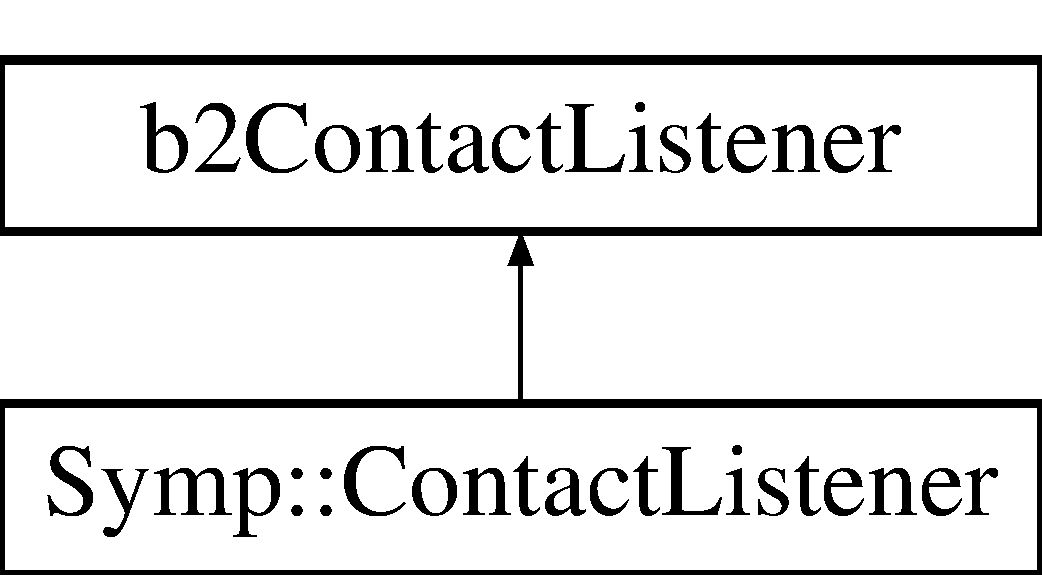
\includegraphics[height=2.000000cm]{class_symp_1_1_contact_listener}
\end{center}
\end{figure}
\subsection*{Public Member Functions}
\begin{DoxyCompactItemize}
\item 
void \hyperlink{class_symp_1_1_contact_listener_ac844c99241a9f3c79da93c2a0ddda381}{Begin\-Contact} (b2\-Contact $\ast$contact)
\item 
void \hyperlink{class_symp_1_1_contact_listener_ad98d5750313af5ace3d39f1affaaafbd}{End\-Contact} (b2\-Contact $\ast$contact)
\end{DoxyCompactItemize}


\subsection{Detailed Description}
This subclass of b2\-Contact\-Listener contains functions called by the \hyperlink{class_symp_1_1_physical_world}{Physical\-World} (more precisely the b2\-World) when there is any contact between physical entities (more precisely b2\-Body). 

Definition at line 16 of file Contact\-Listener.\-h.



\subsection{Member Function Documentation}
\hypertarget{class_symp_1_1_contact_listener_ac844c99241a9f3c79da93c2a0ddda381}{\index{Symp\-::\-Contact\-Listener@{Symp\-::\-Contact\-Listener}!Begin\-Contact@{Begin\-Contact}}
\index{Begin\-Contact@{Begin\-Contact}!Symp::ContactListener@{Symp\-::\-Contact\-Listener}}
\subsubsection[{Begin\-Contact}]{\setlength{\rightskip}{0pt plus 5cm}void Symp\-::\-Contact\-Listener\-::\-Begin\-Contact (
\begin{DoxyParamCaption}
\item[{b2\-Contact $\ast$}]{contact}
\end{DoxyParamCaption}
)}}\label{class_symp_1_1_contact_listener_ac844c99241a9f3c79da93c2a0ddda381}
Called when two fixtures begin to touch. 

Definition at line 8 of file Contact\-Listener.\-cpp.

\hypertarget{class_symp_1_1_contact_listener_ad98d5750313af5ace3d39f1affaaafbd}{\index{Symp\-::\-Contact\-Listener@{Symp\-::\-Contact\-Listener}!End\-Contact@{End\-Contact}}
\index{End\-Contact@{End\-Contact}!Symp::ContactListener@{Symp\-::\-Contact\-Listener}}
\subsubsection[{End\-Contact}]{\setlength{\rightskip}{0pt plus 5cm}void Symp\-::\-Contact\-Listener\-::\-End\-Contact (
\begin{DoxyParamCaption}
\item[{b2\-Contact $\ast$}]{contact}
\end{DoxyParamCaption}
)}}\label{class_symp_1_1_contact_listener_ad98d5750313af5ace3d39f1affaaafbd}
Called when two fixtures cease to touch. 

Definition at line 112 of file Contact\-Listener.\-cpp.



The documentation for this class was generated from the following files\-:\begin{DoxyCompactItemize}
\item 
/home/cecilia/\-Documents/\-Symptogen/src/physic/\hyperlink{_contact_listener_8h}{Contact\-Listener.\-h}\item 
/home/cecilia/\-Documents/\-Symptogen/src/physic/\hyperlink{_contact_listener_8cpp}{Contact\-Listener.\-cpp}\end{DoxyCompactItemize}

\hypertarget{class_symp_1_1_entity_manager}{\section{Symp\-:\-:Entity\-Manager Class Reference}
\label{class_symp_1_1_entity_manager}\index{Symp\-::\-Entity\-Manager@{Symp\-::\-Entity\-Manager}}
}


{\ttfamily \#include $<$Entity\-Manager.\-h$>$}

Inheritance diagram for Symp\-:\-:Entity\-Manager\-:\begin{figure}[H]
\begin{center}
\leavevmode
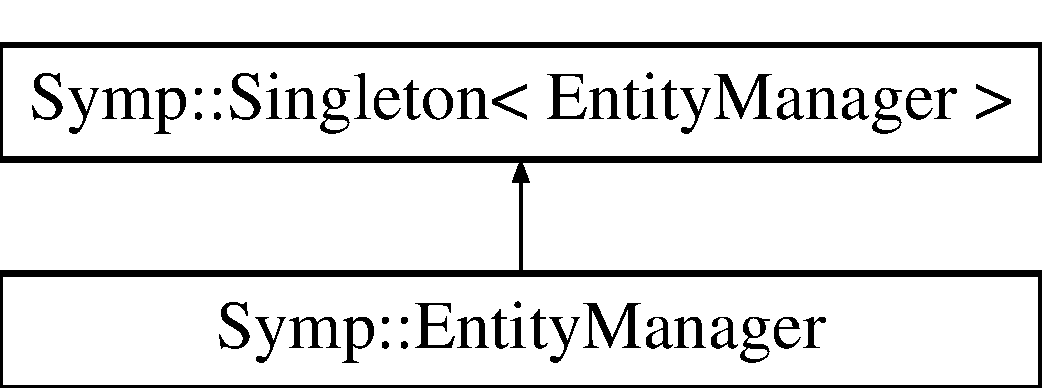
\includegraphics[height=2.000000cm]{class_symp_1_1_entity_manager}
\end{center}
\end{figure}
\subsection*{Public Member Functions}
\begin{DoxyCompactItemize}
\item 
void \hyperlink{class_symp_1_1_entity_manager_a73170f4bf6eb9fcf6519aef64c582f00}{init\-Render} (\hyperlink{class_symp_1_1_render}{Render} $\ast$p\-Render)
\item 
void \hyperlink{class_symp_1_1_entity_manager_ac5c8ac7c5e75bbfce6fc6fe227f2272e}{destroy\-Render} ()
\item 
bool \hyperlink{class_symp_1_1_entity_manager_aaacf8aa937946a64cf2edb6bb35e90d7}{add\-Entity} (std\-::vector$<$ \hyperlink{class_symp_1_1_render_entity}{Render\-Entity} $\ast$ $>$ render\-Entity\-Array, unsigned int layer, \hyperlink{class_symp_1_1_physical_entity}{Physical\-Entity} $\ast$p\-Physical\-Entity, std\-::vector$<$ \hyperlink{class_symp_1_1_sound_entity}{Sound\-Entity} $\ast$ $>$ p\-Sound\-Entity\-Array)
\item 
bool \hyperlink{class_symp_1_1_entity_manager_a462c7b9c4b1bb4bee60887f17ec151de}{add\-Render\-Entity} (std\-::vector$<$ \hyperlink{class_symp_1_1_render_entity}{Render\-Entity} $\ast$ $>$ render\-Entity\-Array, unsigned int layer)
\item 
bool \hyperlink{class_symp_1_1_entity_manager_a51bad2c8fb3f002ab9c30af538ede256}{add\-Physical\-Entity} (\hyperlink{class_symp_1_1_physical_entity}{Physical\-Entity} $\ast$p\-Physical\-Entity)
\item 
bool \hyperlink{class_symp_1_1_entity_manager_a56ad8bda1790f4fd70b1fef35fcb4cb8}{add\-Sound\-Entity} (std\-::vector$<$ \hyperlink{class_symp_1_1_sound_entity}{Sound\-Entity} $\ast$ $>$ p\-Sound\-Entity\-Array)
\item 
bool \hyperlink{class_symp_1_1_entity_manager_aaad8b492cd6742eb7764698d5293c5ee}{add\-Render\-Entity\-To\-Existing\-Entity} (\hyperlink{class_symp_1_1_render_entity}{Render\-Entity} $\ast$render\-Entity, size\-\_\-t index\-Existing\-Entity)
\item 
bool \hyperlink{class_symp_1_1_entity_manager_acec950a76e33763d3ed87b66546c3fbf}{add\-Sound\-Entity\-To\-Existing\-Entity} (\hyperlink{class_symp_1_1_sound_entity}{Sound\-Entity} $\ast$sound\-Entity, size\-\_\-t index\-Existing\-Entity)
\item 
void \hyperlink{class_symp_1_1_entity_manager_a19ec565ae603d54fa0492c426e48f7fd}{render\-Entities} ()
\item 
void \hyperlink{class_symp_1_1_entity_manager_a9af185fe976d1c84b9e7ab1e2a4b4308}{update\-Entities} ()
\item 
void \hyperlink{class_symp_1_1_entity_manager_aa8823bae832700af54b49e8efe2a8f62}{delete\-All\-Entities} ()
\item 
bool \hyperlink{class_symp_1_1_entity_manager_acbecbcfc80353128a8c752887749c668}{delete\-Entity} (size\-\_\-t index)
\item 
void \hyperlink{class_symp_1_1_entity_manager_a3568cd6b5038905fa338eeeb37021529}{add\-Power} (\hyperlink{class_symp_1_1_power}{Power} $\ast$new\-Power, \hyperlink{namespace_symp_a81b2b15da470e4ace7de6835ebe0f8ba}{Power\-Type} type)
\item 
void \hyperlink{class_symp_1_1_entity_manager_a4c10b6b3f729b60049514a2d96e29270}{execute\-Powers} ()
\item 
void \hyperlink{class_symp_1_1_entity_manager_a06a96fd5af27e6b6eb1b1c2e67345998}{delete\-All\-Powers} ()
\item 
void \hyperlink{class_symp_1_1_entity_manager_a9fa151de7f5145f6990f1ca45aa9fa19}{add\-Dino} (int pos\-X, int pos\-Y, int width)
\item 
void \hyperlink{class_symp_1_1_entity_manager_a7d3e685f1e29720b75d5206d0b96fffb}{kill\-Dino} ()
\item 
void \hyperlink{class_symp_1_1_entity_manager_a233cc9e9f348ac0e8c6818597e58cdbf}{add\-Thermometer} ()
\item 
void \hyperlink{class_symp_1_1_entity_manager_ae1b3fd03c8a01486df734a157c85609f}{add\-Flames} ()
\item 
std\-::vector$<$ std\-::vector\\*
$<$ \hyperlink{class_symp_1_1_render_entity}{Render\-Entity} $\ast$ $>$ $>$ \hyperlink{class_symp_1_1_entity_manager_a0c0cfc745886eab36f21fd504e96eea0}{get\-Render\-Entity\-Array} () const 
\item 
std\-::vector$<$ \hyperlink{class_symp_1_1_physical_entity}{Physical\-Entity} $\ast$ $>$ \hyperlink{class_symp_1_1_entity_manager_a9dac748cf0f913f940031c3afa372dc5}{get\-Physical\-Entity\-Array} () const 
\item 
std\-::vector$<$ std\-::vector\\*
$<$ \hyperlink{class_symp_1_1_sound_entity}{Sound\-Entity} $\ast$ $>$ $>$ \hyperlink{class_symp_1_1_entity_manager_a990d6ecd90a1f69745113bde6ca0f7ce}{get\-Sound\-Entity\-Array} () const 
\item 
std\-::vector$<$ \hyperlink{class_symp_1_1_power}{Power} $\ast$ $>$ \hyperlink{class_symp_1_1_entity_manager_a17a315620fcf4158f8d4d897493ad531}{get\-Powers} () const 
\item 
I\-N\-D\-\_\-\-Entity2d\-Manager $\ast$ \hyperlink{class_symp_1_1_entity_manager_aa1babaa1b11f1a0bcdcf5d7c1fe1d3d9}{get\-I\-N\-D\-\_\-\-Entity2d\-Manager} () const 
\item 
\hyperlink{class_symp_1_1_physical_world}{Physical\-World} $\ast$ \hyperlink{class_symp_1_1_entity_manager_afc649b64f5851802facf34afb1dff150}{get\-Physical\-World} () const 
\item 
size\-\_\-t \hyperlink{class_symp_1_1_entity_manager_adafba7ec7121cfd1e7f187e027b8ed3d}{get\-Nb\-Entities} () const 
\item 
size\-\_\-t \hyperlink{class_symp_1_1_entity_manager_a19b90189de9bb0cf8111eda5ec705b6c}{get\-Nb\-Physical\-Entities} () const 
\item 
std\-::array$<$ float, 2 $>$ \hyperlink{class_symp_1_1_entity_manager_af3cea4bd58d629124c47f851174b7334}{get\-Exit\-Coordinates} () const 
\item 
std\-::vector$<$ \hyperlink{class_symp_1_1_render_entity}{Render\-Entity} $\ast$ $>$ \hyperlink{class_symp_1_1_entity_manager_a21aa2e05e4bd2d526306e173c5ca2381}{get\-Render\-Entity} (size\-\_\-t index) const 
\item 
\hyperlink{class_symp_1_1_physical_entity}{Physical\-Entity} $\ast$ \hyperlink{class_symp_1_1_entity_manager_a11ac1efae3f8651994f01ce9df305393}{get\-Physical\-Entity} (size\-\_\-t index) const 
\item 
std\-::vector$<$ \hyperlink{class_symp_1_1_sound_entity}{Sound\-Entity} $\ast$ $>$ \hyperlink{class_symp_1_1_entity_manager_a95ce86f8088b0ebf5b8d19f427d588ac}{get\-Sound\-Entity} (size\-\_\-t index) const 
\item 
std\-::vector$<$ \hyperlink{class_symp_1_1_render_entity}{Render\-Entity} $\ast$ $>$ \hyperlink{class_symp_1_1_entity_manager_ac1dfb6cba31d95ec8369e7dbb54eac1b}{get\-Render\-Dino} () const 
\item 
\hyperlink{class_symp_1_1_physical_entity}{Physical\-Entity} $\ast$ \hyperlink{class_symp_1_1_entity_manager_a813a586c35f339bf57db018191d893ce}{get\-Physical\-Dino} () const 
\item 
std\-::vector$<$ \hyperlink{class_symp_1_1_sound_entity}{Sound\-Entity} $\ast$ $>$ \hyperlink{class_symp_1_1_entity_manager_a11d90dba29177f8c6c5b597116d4949e}{get\-Sound\-Dino} () const 
\item 
\hyperlink{class_symp_1_1_power}{Power} $\ast$ \hyperlink{class_symp_1_1_entity_manager_a56a75c8ac95c235d4740d61315c841c5}{get\-Power} (\hyperlink{namespace_symp_a81b2b15da470e4ace7de6835ebe0f8ba}{Power\-Type} power\-Type) const 
\item 
bool \hyperlink{class_symp_1_1_entity_manager_a49fa79a733f9a075807cacd69b5b8e75}{is\-Power\-Existing} (\hyperlink{namespace_symp_a81b2b15da470e4ace7de6835ebe0f8ba}{Power\-Type} power\-Type) const 
\item 
size\-\_\-t \hyperlink{class_symp_1_1_entity_manager_a9009e9467ce9240176f37041531f1f53}{get\-Index\-Entity} (\hyperlink{class_symp_1_1_physical_entity}{Physical\-Entity} $\ast$p\-Physical\-Entity) const 
\item 
size\-\_\-t \hyperlink{class_symp_1_1_entity_manager_a120b298f2703eef7973e123a67c9bcdd}{get\-Index\-Entity\-From\-Render\-Entity} (std\-::vector$<$ \hyperlink{class_symp_1_1_render_entity}{Render\-Entity} $\ast$ $>$ p\-Render\-Entity\-Array) const 
\item 
\hyperlink{namespace_symp_a303925db810fa122d017c4001bfa5e88}{Dino\-Action} \hyperlink{class_symp_1_1_entity_manager_af68a927c11f97d6bedb3e4f1d24b7113}{get\-Current\-Dino\-Action} () const 
\item 
\hyperlink{namespace_symp_a81b2b15da470e4ace7de6835ebe0f8ba}{Power\-Type} \hyperlink{class_symp_1_1_entity_manager_a3d3c399d4194f5c08371b8fa182b11c9}{get\-Current\-Power\-Type} () const 
\item 
\hyperlink{namespace_symp_a7c4a93cb3761077f6b73ebce19c562c1}{Power\-State} \hyperlink{class_symp_1_1_entity_manager_a0649f2b3f065f7ffd9457b3401b78146}{get\-Current\-Power\-State} () const 
\item 
bool \hyperlink{class_symp_1_1_entity_manager_a78c7feee11012871c2e0bf11f9c7f9d3}{is\-Dino\-Allow\-To\-Move} ()
\item 
bool \hyperlink{class_symp_1_1_entity_manager_a530f46316832cbe3f39278a80b41a0de}{is\-Dino\-Allow\-To\-Jump} ()
\item 
bool \hyperlink{class_symp_1_1_entity_manager_a5b5a53c52b7f2133e74f910320ee3203}{is\-Death\-Animation\-Playing} ()
\item 
\hyperlink{namespace_symp_a303925db810fa122d017c4001bfa5e88}{Dino\-Action} \hyperlink{class_symp_1_1_entity_manager_a7c72832895e29e4eb5f77d6ab0fe58d2}{get\-Right\-Death} ()
\item 
\hyperlink{namespace_symp_a303925db810fa122d017c4001bfa5e88}{Dino\-Action} \hyperlink{class_symp_1_1_entity_manager_a3ce38be311a9d0712d3b8713eb5f76e8}{get\-Right\-Walk} ()
\item 
\hyperlink{namespace_symp_a303925db810fa122d017c4001bfa5e88}{Dino\-Action} \hyperlink{class_symp_1_1_entity_manager_a43d0eb59800de0b2422b5b0f95d2c08f}{get\-Right\-Stop} ()
\item 
bool \hyperlink{class_symp_1_1_entity_manager_a52b4c798c895aa7f77ce228107f1d6c8}{get\-Is\-Dino\-Shivering} ()
\item 
void \hyperlink{class_symp_1_1_entity_manager_abc616919576f3f934b0a3a894fbf73ce}{set\-Exit\-Coordinates} (float pos\-X, float pos\-Y)
\item 
void \hyperlink{class_symp_1_1_entity_manager_af4c4ae3b2fbbaf6d8230a581928533a5}{set\-Dino\-Render} (\hyperlink{namespace_symp_a303925db810fa122d017c4001bfa5e88}{Dino\-Action} dino\-Action)
\item 
void \hyperlink{class_symp_1_1_entity_manager_aee82c43f4077bafd9bab82afebde8c52}{flip\-Dino\-Render\-Entities} (bool flip)
\item 
void \hyperlink{class_symp_1_1_entity_manager_a0688e53ec03ddb4175b373575c5e0054}{set\-Flower\-Render} (size\-\_\-t index, \hyperlink{namespace_symp_a2b868de1f6f86f455f39dfa63028859c}{Flower\-Action} action)
\item 
void \hyperlink{class_symp_1_1_entity_manager_a97c9577c4f459e3a08465caf45f25853}{set\-Destructible\-Object\-Render} (size\-\_\-t index, \hyperlink{namespace_symp_a9f891c0e98f2864e7b687d741bf032d7}{Destructible\-Object\-Action} action)
\item 
void \hyperlink{class_symp_1_1_entity_manager_a1dd7c6251093f5d6cd64460916c8cbbb}{update\-Thermomether\-Render} ()
\item 
void \hyperlink{class_symp_1_1_entity_manager_a4df159993061bc3098f6861f715a17c1}{update\-Flames} ()
\item 
void \hyperlink{class_symp_1_1_entity_manager_af4d70469e46f2c8473aa877e1acff635}{update\-Destructible\-Objects} ()
\item 
void \hyperlink{class_symp_1_1_entity_manager_a555efd00fbf09f062b22f463d49a6e22}{set\-Is\-Dino\-Shivering} (bool shiver)
\end{DoxyCompactItemize}
\subsection*{Friends}
\begin{DoxyCompactItemize}
\item 
class \hyperlink{class_symp_1_1_entity_manager_a275303a889d60f5019ba1b3f2d529c6b}{Singleton$<$ Entity\-Manager $>$}
\end{DoxyCompactItemize}
\subsection*{Additional Inherited Members}


\subsection{Detailed Description}
Manages all the entites of the game(of any type). It is a singleton. It has the knowledge of all entities which exist at a specific moment. It provides tools to \-:
\begin{DoxyItemize}
\item Add entities
\item Update entities
\item Delete entitites 
\end{DoxyItemize}

Definition at line 80 of file Entity\-Manager.\-h.



\subsection{Member Function Documentation}
\hypertarget{class_symp_1_1_entity_manager_a9fa151de7f5145f6990f1ca45aa9fa19}{\index{Symp\-::\-Entity\-Manager@{Symp\-::\-Entity\-Manager}!add\-Dino@{add\-Dino}}
\index{add\-Dino@{add\-Dino}!Symp::EntityManager@{Symp\-::\-Entity\-Manager}}
\subsubsection[{add\-Dino}]{\setlength{\rightskip}{0pt plus 5cm}void Symp\-::\-Entity\-Manager\-::add\-Dino (
\begin{DoxyParamCaption}
\item[{int}]{pos\-X, }
\item[{int}]{pos\-Y, }
\item[{int}]{width}
\end{DoxyParamCaption}
)}}\label{class_symp_1_1_entity_manager_a9fa151de7f5145f6990f1ca45aa9fa19}
Add all needed entities for the dino (render, physical, and sound). 
\begin{DoxyParams}{Parameters}
{\em pos\-X} & \-: the X position of the center of the dino we want to create \\
\hline
{\em pos\-Y} & \-: the Y position of the center of the dino we want to create \\
\hline
{\em width} & \-: the width of the dino we want to create. The width is setted automaticaly. \\
\hline
\end{DoxyParams}


Definition at line 273 of file Entity\-Manager.\-cpp.

\hypertarget{class_symp_1_1_entity_manager_aaacf8aa937946a64cf2edb6bb35e90d7}{\index{Symp\-::\-Entity\-Manager@{Symp\-::\-Entity\-Manager}!add\-Entity@{add\-Entity}}
\index{add\-Entity@{add\-Entity}!Symp::EntityManager@{Symp\-::\-Entity\-Manager}}
\subsubsection[{add\-Entity}]{\setlength{\rightskip}{0pt plus 5cm}bool Symp\-::\-Entity\-Manager\-::add\-Entity (
\begin{DoxyParamCaption}
\item[{std\-::vector$<$ {\bf Render\-Entity} $\ast$ $>$}]{render\-Entity\-Array, }
\item[{unsigned int}]{layer, }
\item[{{\bf Physical\-Entity} $\ast$}]{p\-Physical\-Entity, }
\item[{std\-::vector$<$ {\bf Sound\-Entity} $\ast$ $>$}]{p\-Sound\-Entity\-Array}
\end{DoxyParamCaption}
)}}\label{class_symp_1_1_entity_manager_aaacf8aa937946a64cf2edb6bb35e90d7}
Adds a new entity. Pushes back one object of each entity type in the corresponding array. If the entity does not specify a component, the value of the object is set to a N\-U\-L\-L. The layer parameter corresponds to the layer in which the render entity has to be displayed (cf \-: \hyperlink{class_symp_1_1_render}{Render}). \begin{DoxySeeAlso}{See Also}
\hyperlink{class_symp_1_1_entity_manager_aaacf8aa937946a64cf2edb6bb35e90d7}{add\-Entity()} 
\end{DoxySeeAlso}

\begin{DoxyParams}{Parameters}
{\em render\-Entity\-Array} & \-: array of all rendering corresponding to the entity \\
\hline
{\em layer} & \-: layer of the render entity \\
\hline
{\em p\-Physical\-Entity,\-:} & physical entity  p\-Sound\-Entity\-Array \-: array of all sounds corresponding to the entity \\
\hline
\end{DoxyParams}
\begin{DoxyReturn}{Returns}
boolean that indicates if the entity has been added correctly 
\end{DoxyReturn}


Definition at line 62 of file Entity\-Manager.\-cpp.

\hypertarget{class_symp_1_1_entity_manager_ae1b3fd03c8a01486df734a157c85609f}{\index{Symp\-::\-Entity\-Manager@{Symp\-::\-Entity\-Manager}!add\-Flames@{add\-Flames}}
\index{add\-Flames@{add\-Flames}!Symp::EntityManager@{Symp\-::\-Entity\-Manager}}
\subsubsection[{add\-Flames}]{\setlength{\rightskip}{0pt plus 5cm}void Symp\-::\-Entity\-Manager\-::add\-Flames (
\begin{DoxyParamCaption}
{}
\end{DoxyParamCaption}
)}}\label{class_symp_1_1_entity_manager_ae1b3fd03c8a01486df734a157c85609f}
Add all needed entities for the flames (when hot fever) \-: render and physic. 

Definition at line 499 of file Entity\-Manager.\-cpp.

\hypertarget{class_symp_1_1_entity_manager_a51bad2c8fb3f002ab9c30af538ede256}{\index{Symp\-::\-Entity\-Manager@{Symp\-::\-Entity\-Manager}!add\-Physical\-Entity@{add\-Physical\-Entity}}
\index{add\-Physical\-Entity@{add\-Physical\-Entity}!Symp::EntityManager@{Symp\-::\-Entity\-Manager}}
\subsubsection[{add\-Physical\-Entity}]{\setlength{\rightskip}{0pt plus 5cm}bool Symp\-::\-Entity\-Manager\-::add\-Physical\-Entity (
\begin{DoxyParamCaption}
\item[{{\bf Physical\-Entity} $\ast$}]{p\-Physical\-Entity}
\end{DoxyParamCaption}
)}}\label{class_symp_1_1_entity_manager_a51bad2c8fb3f002ab9c30af538ede256}
Adds a new physical entity The render\-Entity and sound\-Entity components are set to N\-U\-L\-L \begin{DoxySeeAlso}{See Also}
\hyperlink{class_symp_1_1_entity_manager_aaacf8aa937946a64cf2edb6bb35e90d7}{add\-Entity()} 

\hyperlink{class_symp_1_1_entity_manager_a462c7b9c4b1bb4bee60887f17ec151de}{add\-Render\-Entity()} 

\hyperlink{class_symp_1_1_entity_manager_a56ad8bda1790f4fd70b1fef35fcb4cb8}{add\-Sound\-Entity()} 
\end{DoxySeeAlso}

\begin{DoxyParams}{Parameters}
{\em p\-Physical\-Entity} & \-: physical entity \\
\hline
\end{DoxyParams}
\begin{DoxyReturn}{Returns}
boolean that indicates if the entity has been added correctly 
\end{DoxyReturn}


Definition at line 48 of file Entity\-Manager.\-cpp.

\hypertarget{class_symp_1_1_entity_manager_a3568cd6b5038905fa338eeeb37021529}{\index{Symp\-::\-Entity\-Manager@{Symp\-::\-Entity\-Manager}!add\-Power@{add\-Power}}
\index{add\-Power@{add\-Power}!Symp::EntityManager@{Symp\-::\-Entity\-Manager}}
\subsubsection[{add\-Power}]{\setlength{\rightskip}{0pt plus 5cm}void Symp\-::\-Entity\-Manager\-::add\-Power (
\begin{DoxyParamCaption}
\item[{{\bf Power} $\ast$}]{new\-Power, }
\item[{{\bf Power\-Type}}]{type}
\end{DoxyParamCaption}
)}}\label{class_symp_1_1_entity_manager_a3568cd6b5038905fa338eeeb37021529}
Add a power to the list of power 

Definition at line 249 of file Entity\-Manager.\-cpp.

\hypertarget{class_symp_1_1_entity_manager_a462c7b9c4b1bb4bee60887f17ec151de}{\index{Symp\-::\-Entity\-Manager@{Symp\-::\-Entity\-Manager}!add\-Render\-Entity@{add\-Render\-Entity}}
\index{add\-Render\-Entity@{add\-Render\-Entity}!Symp::EntityManager@{Symp\-::\-Entity\-Manager}}
\subsubsection[{add\-Render\-Entity}]{\setlength{\rightskip}{0pt plus 5cm}bool Symp\-::\-Entity\-Manager\-::add\-Render\-Entity (
\begin{DoxyParamCaption}
\item[{std\-::vector$<$ {\bf Render\-Entity} $\ast$ $>$}]{render\-Entity\-Array, }
\item[{unsigned int}]{layer}
\end{DoxyParamCaption}
)}}\label{class_symp_1_1_entity_manager_a462c7b9c4b1bb4bee60887f17ec151de}
Adds a new render entity The physical\-Entity and sound\-Entity components are set to N\-U\-L\-L \begin{DoxySeeAlso}{See Also}
\hyperlink{class_symp_1_1_entity_manager_aaacf8aa937946a64cf2edb6bb35e90d7}{add\-Entity()} 

\hyperlink{class_symp_1_1_entity_manager_a51bad2c8fb3f002ab9c30af538ede256}{add\-Physical\-Entity()} 

\hyperlink{class_symp_1_1_entity_manager_a56ad8bda1790f4fd70b1fef35fcb4cb8}{add\-Sound\-Entity()} 
\end{DoxySeeAlso}

\begin{DoxyParams}{Parameters}
{\em render\-Entity\-Array} & \-: array of all rendering corresponding to the entity \\
\hline
{\em layer} & \-: layder of the render entity \\
\hline
\end{DoxyParams}
\begin{DoxyReturn}{Returns}
boolean that indicates if the entity has been added correctly 
\end{DoxyReturn}


Definition at line 38 of file Entity\-Manager.\-cpp.

\hypertarget{class_symp_1_1_entity_manager_aaad8b492cd6742eb7764698d5293c5ee}{\index{Symp\-::\-Entity\-Manager@{Symp\-::\-Entity\-Manager}!add\-Render\-Entity\-To\-Existing\-Entity@{add\-Render\-Entity\-To\-Existing\-Entity}}
\index{add\-Render\-Entity\-To\-Existing\-Entity@{add\-Render\-Entity\-To\-Existing\-Entity}!Symp::EntityManager@{Symp\-::\-Entity\-Manager}}
\subsubsection[{add\-Render\-Entity\-To\-Existing\-Entity}]{\setlength{\rightskip}{0pt plus 5cm}bool Symp\-::\-Entity\-Manager\-::add\-Render\-Entity\-To\-Existing\-Entity (
\begin{DoxyParamCaption}
\item[{{\bf Render\-Entity} $\ast$}]{render\-Entity, }
\item[{size\-\_\-t}]{index\-Existing\-Entity}
\end{DoxyParamCaption}
)}}\label{class_symp_1_1_entity_manager_aaad8b492cd6742eb7764698d5293c5ee}
Add a render entity to an existing entity. 

Definition at line 73 of file Entity\-Manager.\-cpp.

\hypertarget{class_symp_1_1_entity_manager_a56ad8bda1790f4fd70b1fef35fcb4cb8}{\index{Symp\-::\-Entity\-Manager@{Symp\-::\-Entity\-Manager}!add\-Sound\-Entity@{add\-Sound\-Entity}}
\index{add\-Sound\-Entity@{add\-Sound\-Entity}!Symp::EntityManager@{Symp\-::\-Entity\-Manager}}
\subsubsection[{add\-Sound\-Entity}]{\setlength{\rightskip}{0pt plus 5cm}bool Symp\-::\-Entity\-Manager\-::add\-Sound\-Entity (
\begin{DoxyParamCaption}
\item[{std\-::vector$<$ {\bf Sound\-Entity} $\ast$ $>$}]{p\-Sound\-Entity\-Array}
\end{DoxyParamCaption}
)}}\label{class_symp_1_1_entity_manager_a56ad8bda1790f4fd70b1fef35fcb4cb8}
Adds a new sound entity The render\-Entity and physical\-Entity components are set to N\-U\-L\-L \begin{DoxySeeAlso}{See Also}
\hyperlink{class_symp_1_1_entity_manager_aaacf8aa937946a64cf2edb6bb35e90d7}{add\-Entity()} 

\hyperlink{class_symp_1_1_entity_manager_a462c7b9c4b1bb4bee60887f17ec151de}{add\-Render\-Entity()} 

\hyperlink{class_symp_1_1_entity_manager_a51bad2c8fb3f002ab9c30af538ede256}{add\-Physical\-Entity()} 
\end{DoxySeeAlso}

\begin{DoxyParams}{Parameters}
{\em p\-Sound\-Entity\-Array} & \-: array of all sounds corresponding to the entity \\
\hline
\end{DoxyParams}
\begin{DoxyReturn}{Returns}
boolean that indicates if the entity has been added correctly 
\end{DoxyReturn}


Definition at line 55 of file Entity\-Manager.\-cpp.

\hypertarget{class_symp_1_1_entity_manager_acec950a76e33763d3ed87b66546c3fbf}{\index{Symp\-::\-Entity\-Manager@{Symp\-::\-Entity\-Manager}!add\-Sound\-Entity\-To\-Existing\-Entity@{add\-Sound\-Entity\-To\-Existing\-Entity}}
\index{add\-Sound\-Entity\-To\-Existing\-Entity@{add\-Sound\-Entity\-To\-Existing\-Entity}!Symp::EntityManager@{Symp\-::\-Entity\-Manager}}
\subsubsection[{add\-Sound\-Entity\-To\-Existing\-Entity}]{\setlength{\rightskip}{0pt plus 5cm}bool Symp\-::\-Entity\-Manager\-::add\-Sound\-Entity\-To\-Existing\-Entity (
\begin{DoxyParamCaption}
\item[{{\bf Sound\-Entity} $\ast$}]{sound\-Entity, }
\item[{size\-\_\-t}]{index\-Existing\-Entity}
\end{DoxyParamCaption}
)}}\label{class_symp_1_1_entity_manager_acec950a76e33763d3ed87b66546c3fbf}
Add a sound entity to an existing entity. 

Definition at line 78 of file Entity\-Manager.\-cpp.

\hypertarget{class_symp_1_1_entity_manager_a233cc9e9f348ac0e8c6818597e58cdbf}{\index{Symp\-::\-Entity\-Manager@{Symp\-::\-Entity\-Manager}!add\-Thermometer@{add\-Thermometer}}
\index{add\-Thermometer@{add\-Thermometer}!Symp::EntityManager@{Symp\-::\-Entity\-Manager}}
\subsubsection[{add\-Thermometer}]{\setlength{\rightskip}{0pt plus 5cm}void Symp\-::\-Entity\-Manager\-::add\-Thermometer (
\begin{DoxyParamCaption}
{}
\end{DoxyParamCaption}
)}}\label{class_symp_1_1_entity_manager_a233cc9e9f348ac0e8c6818597e58cdbf}
Add all needed entities for the thermometer (render). 

Definition at line 474 of file Entity\-Manager.\-cpp.

\hypertarget{class_symp_1_1_entity_manager_aa8823bae832700af54b49e8efe2a8f62}{\index{Symp\-::\-Entity\-Manager@{Symp\-::\-Entity\-Manager}!delete\-All\-Entities@{delete\-All\-Entities}}
\index{delete\-All\-Entities@{delete\-All\-Entities}!Symp::EntityManager@{Symp\-::\-Entity\-Manager}}
\subsubsection[{delete\-All\-Entities}]{\setlength{\rightskip}{0pt plus 5cm}void Symp\-::\-Entity\-Manager\-::delete\-All\-Entities (
\begin{DoxyParamCaption}
{}
\end{DoxyParamCaption}
)}}\label{class_symp_1_1_entity_manager_aa8823bae832700af54b49e8efe2a8f62}
Delete all the entities \-: move physics and fit position of render entities on physical entities. 

Definition at line 162 of file Entity\-Manager.\-cpp.

\hypertarget{class_symp_1_1_entity_manager_a06a96fd5af27e6b6eb1b1c2e67345998}{\index{Symp\-::\-Entity\-Manager@{Symp\-::\-Entity\-Manager}!delete\-All\-Powers@{delete\-All\-Powers}}
\index{delete\-All\-Powers@{delete\-All\-Powers}!Symp::EntityManager@{Symp\-::\-Entity\-Manager}}
\subsubsection[{delete\-All\-Powers}]{\setlength{\rightskip}{0pt plus 5cm}void Symp\-::\-Entity\-Manager\-::delete\-All\-Powers (
\begin{DoxyParamCaption}
{}
\end{DoxyParamCaption}
)}}\label{class_symp_1_1_entity_manager_a06a96fd5af27e6b6eb1b1c2e67345998}
Delete all the powers 

Definition at line 260 of file Entity\-Manager.\-cpp.

\hypertarget{class_symp_1_1_entity_manager_acbecbcfc80353128a8c752887749c668}{\index{Symp\-::\-Entity\-Manager@{Symp\-::\-Entity\-Manager}!delete\-Entity@{delete\-Entity}}
\index{delete\-Entity@{delete\-Entity}!Symp::EntityManager@{Symp\-::\-Entity\-Manager}}
\subsubsection[{delete\-Entity}]{\setlength{\rightskip}{0pt plus 5cm}bool Symp\-::\-Entity\-Manager\-::delete\-Entity (
\begin{DoxyParamCaption}
\item[{size\-\_\-t}]{index}
\end{DoxyParamCaption}
)}}\label{class_symp_1_1_entity_manager_acbecbcfc80353128a8c752887749c668}
Delete the entity containes at index 
\begin{DoxyParams}{Parameters}
{\em index} & \-: index of the entity we want to remove \\
\hline
\end{DoxyParams}
\begin{DoxyReturn}{Returns}
boolean is true if the deletion went correctly 
\end{DoxyReturn}


Definition at line 201 of file Entity\-Manager.\-cpp.

\hypertarget{class_symp_1_1_entity_manager_ac5c8ac7c5e75bbfce6fc6fe227f2272e}{\index{Symp\-::\-Entity\-Manager@{Symp\-::\-Entity\-Manager}!destroy\-Render@{destroy\-Render}}
\index{destroy\-Render@{destroy\-Render}!Symp::EntityManager@{Symp\-::\-Entity\-Manager}}
\subsubsection[{destroy\-Render}]{\setlength{\rightskip}{0pt plus 5cm}void Symp\-::\-Entity\-Manager\-::destroy\-Render (
\begin{DoxyParamCaption}
{}
\end{DoxyParamCaption}
)}}\label{class_symp_1_1_entity_manager_ac5c8ac7c5e75bbfce6fc6fe227f2272e}


Definition at line 30 of file Entity\-Manager.\-cpp.

\hypertarget{class_symp_1_1_entity_manager_a4c10b6b3f729b60049514a2d96e29270}{\index{Symp\-::\-Entity\-Manager@{Symp\-::\-Entity\-Manager}!execute\-Powers@{execute\-Powers}}
\index{execute\-Powers@{execute\-Powers}!Symp::EntityManager@{Symp\-::\-Entity\-Manager}}
\subsubsection[{execute\-Powers}]{\setlength{\rightskip}{0pt plus 5cm}void Symp\-::\-Entity\-Manager\-::execute\-Powers (
\begin{DoxyParamCaption}
{}
\end{DoxyParamCaption}
)}}\label{class_symp_1_1_entity_manager_a4c10b6b3f729b60049514a2d96e29270}
Launch the execute function of all power stored in the array m\-\_\-power\-Array 

Definition at line 253 of file Entity\-Manager.\-cpp.

\hypertarget{class_symp_1_1_entity_manager_aee82c43f4077bafd9bab82afebde8c52}{\index{Symp\-::\-Entity\-Manager@{Symp\-::\-Entity\-Manager}!flip\-Dino\-Render\-Entities@{flip\-Dino\-Render\-Entities}}
\index{flip\-Dino\-Render\-Entities@{flip\-Dino\-Render\-Entities}!Symp::EntityManager@{Symp\-::\-Entity\-Manager}}
\subsubsection[{flip\-Dino\-Render\-Entities}]{\setlength{\rightskip}{0pt plus 5cm}void Symp\-::\-Entity\-Manager\-::flip\-Dino\-Render\-Entities (
\begin{DoxyParamCaption}
\item[{bool}]{flip}
\end{DoxyParamCaption}
)}}\label{class_symp_1_1_entity_manager_aee82c43f4077bafd9bab82afebde8c52}
Flip all the Dino render entities. 

Definition at line 775 of file Entity\-Manager.\-cpp.

\hypertarget{class_symp_1_1_entity_manager_af68a927c11f97d6bedb3e4f1d24b7113}{\index{Symp\-::\-Entity\-Manager@{Symp\-::\-Entity\-Manager}!get\-Current\-Dino\-Action@{get\-Current\-Dino\-Action}}
\index{get\-Current\-Dino\-Action@{get\-Current\-Dino\-Action}!Symp::EntityManager@{Symp\-::\-Entity\-Manager}}
\subsubsection[{get\-Current\-Dino\-Action}]{\setlength{\rightskip}{0pt plus 5cm}{\bf Dino\-Action} Symp\-::\-Entity\-Manager\-::get\-Current\-Dino\-Action (
\begin{DoxyParamCaption}
{}
\end{DoxyParamCaption}
) const}}\label{class_symp_1_1_entity_manager_af68a927c11f97d6bedb3e4f1d24b7113}
Return the current Dino\-Action (Stop, Jump, Sneezing...) depending on the \hyperlink{class_symp_1_1_render_entity}{Render\-Entity} shown in the vector$<$\-Render\-Entity$\ast$$>$ of the dino. Return Dino\-Action\-::\-Die if access error in std\-::vector$<$\-Render\-Entity$\ast$$>$ of dino. \begin{DoxySeeAlso}{See Also}
\hyperlink{namespace_symp_a303925db810fa122d017c4001bfa5e88}{Dino\-Action} 
\end{DoxySeeAlso}


Definition at line 686 of file Entity\-Manager.\-cpp.

\hypertarget{class_symp_1_1_entity_manager_a0649f2b3f065f7ffd9457b3401b78146}{\index{Symp\-::\-Entity\-Manager@{Symp\-::\-Entity\-Manager}!get\-Current\-Power\-State@{get\-Current\-Power\-State}}
\index{get\-Current\-Power\-State@{get\-Current\-Power\-State}!Symp::EntityManager@{Symp\-::\-Entity\-Manager}}
\subsubsection[{get\-Current\-Power\-State}]{\setlength{\rightskip}{0pt plus 5cm}{\bf Power\-State} Symp\-::\-Entity\-Manager\-::get\-Current\-Power\-State (
\begin{DoxyParamCaption}
{}
\end{DoxyParamCaption}
) const}}\label{class_symp_1_1_entity_manager_a0649f2b3f065f7ffd9457b3401b78146}


Definition at line 722 of file Entity\-Manager.\-cpp.

\hypertarget{class_symp_1_1_entity_manager_a3d3c399d4194f5c08371b8fa182b11c9}{\index{Symp\-::\-Entity\-Manager@{Symp\-::\-Entity\-Manager}!get\-Current\-Power\-Type@{get\-Current\-Power\-Type}}
\index{get\-Current\-Power\-Type@{get\-Current\-Power\-Type}!Symp::EntityManager@{Symp\-::\-Entity\-Manager}}
\subsubsection[{get\-Current\-Power\-Type}]{\setlength{\rightskip}{0pt plus 5cm}{\bf Power\-Type} Symp\-::\-Entity\-Manager\-::get\-Current\-Power\-Type (
\begin{DoxyParamCaption}
{}
\end{DoxyParamCaption}
) const}}\label{class_symp_1_1_entity_manager_a3d3c399d4194f5c08371b8fa182b11c9}
Return the current Power\-Type (\hyperlink{class_symp_1_1_sneeze}{Sneeze}, \hyperlink{class_symp_1_1_fever}{Fever}, \hyperlink{class_symp_1_1_headache}{Headache}) or Normal if there is no power in execution. If error in this function, return Power\-Type\-::\-Normal\-Type. 

Definition at line 706 of file Entity\-Manager.\-cpp.

\hypertarget{class_symp_1_1_entity_manager_af3cea4bd58d629124c47f851174b7334}{\index{Symp\-::\-Entity\-Manager@{Symp\-::\-Entity\-Manager}!get\-Exit\-Coordinates@{get\-Exit\-Coordinates}}
\index{get\-Exit\-Coordinates@{get\-Exit\-Coordinates}!Symp::EntityManager@{Symp\-::\-Entity\-Manager}}
\subsubsection[{get\-Exit\-Coordinates}]{\setlength{\rightskip}{0pt plus 5cm}std\-::array$<$float, 2$>$ Symp\-::\-Entity\-Manager\-::get\-Exit\-Coordinates (
\begin{DoxyParamCaption}
{}
\end{DoxyParamCaption}
) const\hspace{0.3cm}{\ttfamily [inline]}}}\label{class_symp_1_1_entity_manager_af3cea4bd58d629124c47f851174b7334}


Definition at line 225 of file Entity\-Manager.\-h.

\hypertarget{class_symp_1_1_entity_manager_aa1babaa1b11f1a0bcdcf5d7c1fe1d3d9}{\index{Symp\-::\-Entity\-Manager@{Symp\-::\-Entity\-Manager}!get\-I\-N\-D\-\_\-\-Entity2d\-Manager@{get\-I\-N\-D\-\_\-\-Entity2d\-Manager}}
\index{get\-I\-N\-D\-\_\-\-Entity2d\-Manager@{get\-I\-N\-D\-\_\-\-Entity2d\-Manager}!Symp::EntityManager@{Symp\-::\-Entity\-Manager}}
\subsubsection[{get\-I\-N\-D\-\_\-\-Entity2d\-Manager}]{\setlength{\rightskip}{0pt plus 5cm}I\-N\-D\-\_\-\-Entity2d\-Manager$\ast$ Symp\-::\-Entity\-Manager\-::get\-I\-N\-D\-\_\-\-Entity2d\-Manager (
\begin{DoxyParamCaption}
{}
\end{DoxyParamCaption}
) const\hspace{0.3cm}{\ttfamily [inline]}}}\label{class_symp_1_1_entity_manager_aa1babaa1b11f1a0bcdcf5d7c1fe1d3d9}


Definition at line 221 of file Entity\-Manager.\-h.

\hypertarget{class_symp_1_1_entity_manager_a9009e9467ce9240176f37041531f1f53}{\index{Symp\-::\-Entity\-Manager@{Symp\-::\-Entity\-Manager}!get\-Index\-Entity@{get\-Index\-Entity}}
\index{get\-Index\-Entity@{get\-Index\-Entity}!Symp::EntityManager@{Symp\-::\-Entity\-Manager}}
\subsubsection[{get\-Index\-Entity}]{\setlength{\rightskip}{0pt plus 5cm}size\-\_\-t Symp\-::\-Entity\-Manager\-::get\-Index\-Entity (
\begin{DoxyParamCaption}
\item[{{\bf Physical\-Entity} $\ast$}]{p\-Physical\-Entity}
\end{DoxyParamCaption}
) const}}\label{class_symp_1_1_entity_manager_a9009e9467ce9240176f37041531f1f53}


Definition at line 664 of file Entity\-Manager.\-cpp.

\hypertarget{class_symp_1_1_entity_manager_a120b298f2703eef7973e123a67c9bcdd}{\index{Symp\-::\-Entity\-Manager@{Symp\-::\-Entity\-Manager}!get\-Index\-Entity\-From\-Render\-Entity@{get\-Index\-Entity\-From\-Render\-Entity}}
\index{get\-Index\-Entity\-From\-Render\-Entity@{get\-Index\-Entity\-From\-Render\-Entity}!Symp::EntityManager@{Symp\-::\-Entity\-Manager}}
\subsubsection[{get\-Index\-Entity\-From\-Render\-Entity}]{\setlength{\rightskip}{0pt plus 5cm}size\-\_\-t Symp\-::\-Entity\-Manager\-::get\-Index\-Entity\-From\-Render\-Entity (
\begin{DoxyParamCaption}
\item[{std\-::vector$<$ {\bf Render\-Entity} $\ast$ $>$}]{p\-Render\-Entity\-Array}
\end{DoxyParamCaption}
) const}}\label{class_symp_1_1_entity_manager_a120b298f2703eef7973e123a67c9bcdd}


Definition at line 675 of file Entity\-Manager.\-cpp.

\hypertarget{class_symp_1_1_entity_manager_a52b4c798c895aa7f77ce228107f1d6c8}{\index{Symp\-::\-Entity\-Manager@{Symp\-::\-Entity\-Manager}!get\-Is\-Dino\-Shivering@{get\-Is\-Dino\-Shivering}}
\index{get\-Is\-Dino\-Shivering@{get\-Is\-Dino\-Shivering}!Symp::EntityManager@{Symp\-::\-Entity\-Manager}}
\subsubsection[{get\-Is\-Dino\-Shivering}]{\setlength{\rightskip}{0pt plus 5cm}bool Symp\-::\-Entity\-Manager\-::get\-Is\-Dino\-Shivering (
\begin{DoxyParamCaption}
{}
\end{DoxyParamCaption}
)\hspace{0.3cm}{\ttfamily [inline]}}}\label{class_symp_1_1_entity_manager_a52b4c798c895aa7f77ce228107f1d6c8}


Definition at line 323 of file Entity\-Manager.\-h.

\hypertarget{class_symp_1_1_entity_manager_adafba7ec7121cfd1e7f187e027b8ed3d}{\index{Symp\-::\-Entity\-Manager@{Symp\-::\-Entity\-Manager}!get\-Nb\-Entities@{get\-Nb\-Entities}}
\index{get\-Nb\-Entities@{get\-Nb\-Entities}!Symp::EntityManager@{Symp\-::\-Entity\-Manager}}
\subsubsection[{get\-Nb\-Entities}]{\setlength{\rightskip}{0pt plus 5cm}size\-\_\-t Symp\-::\-Entity\-Manager\-::get\-Nb\-Entities (
\begin{DoxyParamCaption}
{}
\end{DoxyParamCaption}
) const\hspace{0.3cm}{\ttfamily [inline]}}}\label{class_symp_1_1_entity_manager_adafba7ec7121cfd1e7f187e027b8ed3d}


Definition at line 223 of file Entity\-Manager.\-h.

\hypertarget{class_symp_1_1_entity_manager_a19b90189de9bb0cf8111eda5ec705b6c}{\index{Symp\-::\-Entity\-Manager@{Symp\-::\-Entity\-Manager}!get\-Nb\-Physical\-Entities@{get\-Nb\-Physical\-Entities}}
\index{get\-Nb\-Physical\-Entities@{get\-Nb\-Physical\-Entities}!Symp::EntityManager@{Symp\-::\-Entity\-Manager}}
\subsubsection[{get\-Nb\-Physical\-Entities}]{\setlength{\rightskip}{0pt plus 5cm}size\-\_\-t Symp\-::\-Entity\-Manager\-::get\-Nb\-Physical\-Entities (
\begin{DoxyParamCaption}
{}
\end{DoxyParamCaption}
) const\hspace{0.3cm}{\ttfamily [inline]}}}\label{class_symp_1_1_entity_manager_a19b90189de9bb0cf8111eda5ec705b6c}


Definition at line 224 of file Entity\-Manager.\-h.

\hypertarget{class_symp_1_1_entity_manager_a813a586c35f339bf57db018191d893ce}{\index{Symp\-::\-Entity\-Manager@{Symp\-::\-Entity\-Manager}!get\-Physical\-Dino@{get\-Physical\-Dino}}
\index{get\-Physical\-Dino@{get\-Physical\-Dino}!Symp::EntityManager@{Symp\-::\-Entity\-Manager}}
\subsubsection[{get\-Physical\-Dino}]{\setlength{\rightskip}{0pt plus 5cm}{\bf Physical\-Entity} $\ast$ Symp\-::\-Entity\-Manager\-::get\-Physical\-Dino (
\begin{DoxyParamCaption}
{}
\end{DoxyParamCaption}
) const}}\label{class_symp_1_1_entity_manager_a813a586c35f339bf57db018191d893ce}
Return an empty Physical\-Entity$\ast$ if the \hyperlink{class_symp_1_1_physical_entity}{Physical\-Entity} of dino does not exist. Abort the program if access error. 

Definition at line 607 of file Entity\-Manager.\-cpp.

\hypertarget{class_symp_1_1_entity_manager_a11ac1efae3f8651994f01ce9df305393}{\index{Symp\-::\-Entity\-Manager@{Symp\-::\-Entity\-Manager}!get\-Physical\-Entity@{get\-Physical\-Entity}}
\index{get\-Physical\-Entity@{get\-Physical\-Entity}!Symp::EntityManager@{Symp\-::\-Entity\-Manager}}
\subsubsection[{get\-Physical\-Entity}]{\setlength{\rightskip}{0pt plus 5cm}{\bf Physical\-Entity} $\ast$ Symp\-::\-Entity\-Manager\-::get\-Physical\-Entity (
\begin{DoxyParamCaption}
\item[{size\-\_\-t}]{index}
\end{DoxyParamCaption}
) const}}\label{class_symp_1_1_entity_manager_a11ac1efae3f8651994f01ce9df305393}
Return a nullptr if the Physical\-Entity$\ast$ does not exist. 

Definition at line 570 of file Entity\-Manager.\-cpp.

\hypertarget{class_symp_1_1_entity_manager_a9dac748cf0f913f940031c3afa372dc5}{\index{Symp\-::\-Entity\-Manager@{Symp\-::\-Entity\-Manager}!get\-Physical\-Entity\-Array@{get\-Physical\-Entity\-Array}}
\index{get\-Physical\-Entity\-Array@{get\-Physical\-Entity\-Array}!Symp::EntityManager@{Symp\-::\-Entity\-Manager}}
\subsubsection[{get\-Physical\-Entity\-Array}]{\setlength{\rightskip}{0pt plus 5cm}std\-::vector$<${\bf Physical\-Entity}$\ast$$>$ Symp\-::\-Entity\-Manager\-::get\-Physical\-Entity\-Array (
\begin{DoxyParamCaption}
{}
\end{DoxyParamCaption}
) const\hspace{0.3cm}{\ttfamily [inline]}}}\label{class_symp_1_1_entity_manager_a9dac748cf0f913f940031c3afa372dc5}


Definition at line 218 of file Entity\-Manager.\-h.

\hypertarget{class_symp_1_1_entity_manager_afc649b64f5851802facf34afb1dff150}{\index{Symp\-::\-Entity\-Manager@{Symp\-::\-Entity\-Manager}!get\-Physical\-World@{get\-Physical\-World}}
\index{get\-Physical\-World@{get\-Physical\-World}!Symp::EntityManager@{Symp\-::\-Entity\-Manager}}
\subsubsection[{get\-Physical\-World}]{\setlength{\rightskip}{0pt plus 5cm}{\bf Physical\-World}$\ast$ Symp\-::\-Entity\-Manager\-::get\-Physical\-World (
\begin{DoxyParamCaption}
{}
\end{DoxyParamCaption}
) const\hspace{0.3cm}{\ttfamily [inline]}}}\label{class_symp_1_1_entity_manager_afc649b64f5851802facf34afb1dff150}


Definition at line 222 of file Entity\-Manager.\-h.

\hypertarget{class_symp_1_1_entity_manager_a56a75c8ac95c235d4740d61315c841c5}{\index{Symp\-::\-Entity\-Manager@{Symp\-::\-Entity\-Manager}!get\-Power@{get\-Power}}
\index{get\-Power@{get\-Power}!Symp::EntityManager@{Symp\-::\-Entity\-Manager}}
\subsubsection[{get\-Power}]{\setlength{\rightskip}{0pt plus 5cm}{\bf Power} $\ast$ Symp\-::\-Entity\-Manager\-::get\-Power (
\begin{DoxyParamCaption}
\item[{{\bf Power\-Type}}]{power\-Type}
\end{DoxyParamCaption}
) const}}\label{class_symp_1_1_entity_manager_a56a75c8ac95c235d4740d61315c841c5}
Return a nullptr if the Power$\ast$ does not exist. 

Definition at line 643 of file Entity\-Manager.\-cpp.

\hypertarget{class_symp_1_1_entity_manager_a17a315620fcf4158f8d4d897493ad531}{\index{Symp\-::\-Entity\-Manager@{Symp\-::\-Entity\-Manager}!get\-Powers@{get\-Powers}}
\index{get\-Powers@{get\-Powers}!Symp::EntityManager@{Symp\-::\-Entity\-Manager}}
\subsubsection[{get\-Powers}]{\setlength{\rightskip}{0pt plus 5cm}std\-::vector$<${\bf Power}$\ast$$>$ Symp\-::\-Entity\-Manager\-::get\-Powers (
\begin{DoxyParamCaption}
{}
\end{DoxyParamCaption}
) const\hspace{0.3cm}{\ttfamily [inline]}}}\label{class_symp_1_1_entity_manager_a17a315620fcf4158f8d4d897493ad531}


Definition at line 220 of file Entity\-Manager.\-h.

\hypertarget{class_symp_1_1_entity_manager_ac1dfb6cba31d95ec8369e7dbb54eac1b}{\index{Symp\-::\-Entity\-Manager@{Symp\-::\-Entity\-Manager}!get\-Render\-Dino@{get\-Render\-Dino}}
\index{get\-Render\-Dino@{get\-Render\-Dino}!Symp::EntityManager@{Symp\-::\-Entity\-Manager}}
\subsubsection[{get\-Render\-Dino}]{\setlength{\rightskip}{0pt plus 5cm}std\-::vector$<$ {\bf Render\-Entity} $\ast$ $>$ Symp\-::\-Entity\-Manager\-::get\-Render\-Dino (
\begin{DoxyParamCaption}
{}
\end{DoxyParamCaption}
) const}}\label{class_symp_1_1_entity_manager_ac1dfb6cba31d95ec8369e7dbb54eac1b}
Return an empty std\-::vector$<$\-Render\-Entity$\ast$$>$ if the \hyperlink{class_symp_1_1_render_entity}{Render\-Entity} of dino does not exist. Abort the program if access error. 

Definition at line 589 of file Entity\-Manager.\-cpp.

\hypertarget{class_symp_1_1_entity_manager_a21aa2e05e4bd2d526306e173c5ca2381}{\index{Symp\-::\-Entity\-Manager@{Symp\-::\-Entity\-Manager}!get\-Render\-Entity@{get\-Render\-Entity}}
\index{get\-Render\-Entity@{get\-Render\-Entity}!Symp::EntityManager@{Symp\-::\-Entity\-Manager}}
\subsubsection[{get\-Render\-Entity}]{\setlength{\rightskip}{0pt plus 5cm}std\-::vector$<$ {\bf Render\-Entity} $\ast$ $>$ Symp\-::\-Entity\-Manager\-::get\-Render\-Entity (
\begin{DoxyParamCaption}
\item[{size\-\_\-t}]{index}
\end{DoxyParamCaption}
) const}}\label{class_symp_1_1_entity_manager_a21aa2e05e4bd2d526306e173c5ca2381}
Return an empty std\-::vector$<$\-Render\-Entity$\ast$$>$ if the \hyperlink{class_symp_1_1_render_entity}{Render\-Entity} does not exist. 

Definition at line 560 of file Entity\-Manager.\-cpp.

\hypertarget{class_symp_1_1_entity_manager_a0c0cfc745886eab36f21fd504e96eea0}{\index{Symp\-::\-Entity\-Manager@{Symp\-::\-Entity\-Manager}!get\-Render\-Entity\-Array@{get\-Render\-Entity\-Array}}
\index{get\-Render\-Entity\-Array@{get\-Render\-Entity\-Array}!Symp::EntityManager@{Symp\-::\-Entity\-Manager}}
\subsubsection[{get\-Render\-Entity\-Array}]{\setlength{\rightskip}{0pt plus 5cm}std\-::vector$<$std\-::vector$<${\bf Render\-Entity}$\ast$$>$ $>$ Symp\-::\-Entity\-Manager\-::get\-Render\-Entity\-Array (
\begin{DoxyParamCaption}
{}
\end{DoxyParamCaption}
) const\hspace{0.3cm}{\ttfamily [inline]}}}\label{class_symp_1_1_entity_manager_a0c0cfc745886eab36f21fd504e96eea0}


Definition at line 217 of file Entity\-Manager.\-h.

\hypertarget{class_symp_1_1_entity_manager_a7c72832895e29e4eb5f77d6ab0fe58d2}{\index{Symp\-::\-Entity\-Manager@{Symp\-::\-Entity\-Manager}!get\-Right\-Death@{get\-Right\-Death}}
\index{get\-Right\-Death@{get\-Right\-Death}!Symp::EntityManager@{Symp\-::\-Entity\-Manager}}
\subsubsection[{get\-Right\-Death}]{\setlength{\rightskip}{0pt plus 5cm}{\bf Dino\-Action} Symp\-::\-Entity\-Manager\-::get\-Right\-Death (
\begin{DoxyParamCaption}
{}
\end{DoxyParamCaption}
)}}\label{class_symp_1_1_entity_manager_a7c72832895e29e4eb5f77d6ab0fe58d2}
Determine the right death animation to play 

Definition at line 905 of file Entity\-Manager.\-cpp.

\hypertarget{class_symp_1_1_entity_manager_a43d0eb59800de0b2422b5b0f95d2c08f}{\index{Symp\-::\-Entity\-Manager@{Symp\-::\-Entity\-Manager}!get\-Right\-Stop@{get\-Right\-Stop}}
\index{get\-Right\-Stop@{get\-Right\-Stop}!Symp::EntityManager@{Symp\-::\-Entity\-Manager}}
\subsubsection[{get\-Right\-Stop}]{\setlength{\rightskip}{0pt plus 5cm}{\bf Dino\-Action} Symp\-::\-Entity\-Manager\-::get\-Right\-Stop (
\begin{DoxyParamCaption}
{}
\end{DoxyParamCaption}
)}}\label{class_symp_1_1_entity_manager_a43d0eb59800de0b2422b5b0f95d2c08f}
Determine the right stop animation to play 

Definition at line 962 of file Entity\-Manager.\-cpp.

\hypertarget{class_symp_1_1_entity_manager_a3ce38be311a9d0712d3b8713eb5f76e8}{\index{Symp\-::\-Entity\-Manager@{Symp\-::\-Entity\-Manager}!get\-Right\-Walk@{get\-Right\-Walk}}
\index{get\-Right\-Walk@{get\-Right\-Walk}!Symp::EntityManager@{Symp\-::\-Entity\-Manager}}
\subsubsection[{get\-Right\-Walk}]{\setlength{\rightskip}{0pt plus 5cm}{\bf Dino\-Action} Symp\-::\-Entity\-Manager\-::get\-Right\-Walk (
\begin{DoxyParamCaption}
{}
\end{DoxyParamCaption}
)}}\label{class_symp_1_1_entity_manager_a3ce38be311a9d0712d3b8713eb5f76e8}
Determine the right walk animation to play 

Definition at line 921 of file Entity\-Manager.\-cpp.

\hypertarget{class_symp_1_1_entity_manager_a11d90dba29177f8c6c5b597116d4949e}{\index{Symp\-::\-Entity\-Manager@{Symp\-::\-Entity\-Manager}!get\-Sound\-Dino@{get\-Sound\-Dino}}
\index{get\-Sound\-Dino@{get\-Sound\-Dino}!Symp::EntityManager@{Symp\-::\-Entity\-Manager}}
\subsubsection[{get\-Sound\-Dino}]{\setlength{\rightskip}{0pt plus 5cm}std\-::vector$<$ {\bf Sound\-Entity} $\ast$ $>$ Symp\-::\-Entity\-Manager\-::get\-Sound\-Dino (
\begin{DoxyParamCaption}
{}
\end{DoxyParamCaption}
) const}}\label{class_symp_1_1_entity_manager_a11d90dba29177f8c6c5b597116d4949e}
Return an empty std\-::vector$<$\-Sound\-Entity$\ast$$>$ if the \hyperlink{class_symp_1_1_sound_entity}{Sound\-Entity} of dino does not exist. Abort the program if access error. 

Definition at line 625 of file Entity\-Manager.\-cpp.

\hypertarget{class_symp_1_1_entity_manager_a95ce86f8088b0ebf5b8d19f427d588ac}{\index{Symp\-::\-Entity\-Manager@{Symp\-::\-Entity\-Manager}!get\-Sound\-Entity@{get\-Sound\-Entity}}
\index{get\-Sound\-Entity@{get\-Sound\-Entity}!Symp::EntityManager@{Symp\-::\-Entity\-Manager}}
\subsubsection[{get\-Sound\-Entity}]{\setlength{\rightskip}{0pt plus 5cm}std\-::vector$<$ {\bf Sound\-Entity} $\ast$ $>$ Symp\-::\-Entity\-Manager\-::get\-Sound\-Entity (
\begin{DoxyParamCaption}
\item[{size\-\_\-t}]{index}
\end{DoxyParamCaption}
) const}}\label{class_symp_1_1_entity_manager_a95ce86f8088b0ebf5b8d19f427d588ac}
Return an empty std\-::vector$<$\-Sound\-Entity$\ast$$>$ if the \hyperlink{class_symp_1_1_sound_entity}{Sound\-Entity} does not exist. 

Definition at line 579 of file Entity\-Manager.\-cpp.

\hypertarget{class_symp_1_1_entity_manager_a990d6ecd90a1f69745113bde6ca0f7ce}{\index{Symp\-::\-Entity\-Manager@{Symp\-::\-Entity\-Manager}!get\-Sound\-Entity\-Array@{get\-Sound\-Entity\-Array}}
\index{get\-Sound\-Entity\-Array@{get\-Sound\-Entity\-Array}!Symp::EntityManager@{Symp\-::\-Entity\-Manager}}
\subsubsection[{get\-Sound\-Entity\-Array}]{\setlength{\rightskip}{0pt plus 5cm}std\-::vector$<$std\-::vector$<${\bf Sound\-Entity}$\ast$$>$ $>$ Symp\-::\-Entity\-Manager\-::get\-Sound\-Entity\-Array (
\begin{DoxyParamCaption}
{}
\end{DoxyParamCaption}
) const\hspace{0.3cm}{\ttfamily [inline]}}}\label{class_symp_1_1_entity_manager_a990d6ecd90a1f69745113bde6ca0f7ce}


Definition at line 219 of file Entity\-Manager.\-h.

\hypertarget{class_symp_1_1_entity_manager_a73170f4bf6eb9fcf6519aef64c582f00}{\index{Symp\-::\-Entity\-Manager@{Symp\-::\-Entity\-Manager}!init\-Render@{init\-Render}}
\index{init\-Render@{init\-Render}!Symp::EntityManager@{Symp\-::\-Entity\-Manager}}
\subsubsection[{init\-Render}]{\setlength{\rightskip}{0pt plus 5cm}void Symp\-::\-Entity\-Manager\-::init\-Render (
\begin{DoxyParamCaption}
\item[{{\bf Render} $\ast$}]{p\-Render}
\end{DoxyParamCaption}
)}}\label{class_symp_1_1_entity_manager_a73170f4bf6eb9fcf6519aef64c582f00}


Definition at line 23 of file Entity\-Manager.\-cpp.

\hypertarget{class_symp_1_1_entity_manager_a5b5a53c52b7f2133e74f910320ee3203}{\index{Symp\-::\-Entity\-Manager@{Symp\-::\-Entity\-Manager}!is\-Death\-Animation\-Playing@{is\-Death\-Animation\-Playing}}
\index{is\-Death\-Animation\-Playing@{is\-Death\-Animation\-Playing}!Symp::EntityManager@{Symp\-::\-Entity\-Manager}}
\subsubsection[{is\-Death\-Animation\-Playing}]{\setlength{\rightskip}{0pt plus 5cm}bool Symp\-::\-Entity\-Manager\-::is\-Death\-Animation\-Playing (
\begin{DoxyParamCaption}
{}
\end{DoxyParamCaption}
)}}\label{class_symp_1_1_entity_manager_a5b5a53c52b7f2133e74f910320ee3203}
Return true if a death animation is playing, else false 

Definition at line 896 of file Entity\-Manager.\-cpp.

\hypertarget{class_symp_1_1_entity_manager_a530f46316832cbe3f39278a80b41a0de}{\index{Symp\-::\-Entity\-Manager@{Symp\-::\-Entity\-Manager}!is\-Dino\-Allow\-To\-Jump@{is\-Dino\-Allow\-To\-Jump}}
\index{is\-Dino\-Allow\-To\-Jump@{is\-Dino\-Allow\-To\-Jump}!Symp::EntityManager@{Symp\-::\-Entity\-Manager}}
\subsubsection[{is\-Dino\-Allow\-To\-Jump}]{\setlength{\rightskip}{0pt plus 5cm}bool Symp\-::\-Entity\-Manager\-::is\-Dino\-Allow\-To\-Jump (
\begin{DoxyParamCaption}
{}
\end{DoxyParamCaption}
)}}\label{class_symp_1_1_entity_manager_a530f46316832cbe3f39278a80b41a0de}
This is a patch for Box2\-D problems when a shape end a contact of begin a new one very quicky (the jump can be unlimited). 

Definition at line 754 of file Entity\-Manager.\-cpp.

\hypertarget{class_symp_1_1_entity_manager_a78c7feee11012871c2e0bf11f9c7f9d3}{\index{Symp\-::\-Entity\-Manager@{Symp\-::\-Entity\-Manager}!is\-Dino\-Allow\-To\-Move@{is\-Dino\-Allow\-To\-Move}}
\index{is\-Dino\-Allow\-To\-Move@{is\-Dino\-Allow\-To\-Move}!Symp::EntityManager@{Symp\-::\-Entity\-Manager}}
\subsubsection[{is\-Dino\-Allow\-To\-Move}]{\setlength{\rightskip}{0pt plus 5cm}bool Symp\-::\-Entity\-Manager\-::is\-Dino\-Allow\-To\-Move (
\begin{DoxyParamCaption}
{}
\end{DoxyParamCaption}
)}}\label{class_symp_1_1_entity_manager_a78c7feee11012871c2e0bf11f9c7f9d3}
The dino can't move when the sneeze power is activate. The dino can't move when the sneeze power is activate. 

Definition at line 746 of file Entity\-Manager.\-cpp.

\hypertarget{class_symp_1_1_entity_manager_a49fa79a733f9a075807cacd69b5b8e75}{\index{Symp\-::\-Entity\-Manager@{Symp\-::\-Entity\-Manager}!is\-Power\-Existing@{is\-Power\-Existing}}
\index{is\-Power\-Existing@{is\-Power\-Existing}!Symp::EntityManager@{Symp\-::\-Entity\-Manager}}
\subsubsection[{is\-Power\-Existing}]{\setlength{\rightskip}{0pt plus 5cm}bool Symp\-::\-Entity\-Manager\-::is\-Power\-Existing (
\begin{DoxyParamCaption}
\item[{{\bf Power\-Type}}]{power\-Type}
\end{DoxyParamCaption}
) const}}\label{class_symp_1_1_entity_manager_a49fa79a733f9a075807cacd69b5b8e75}
Return false if the Power$\ast$ does not exist. 

Definition at line 653 of file Entity\-Manager.\-cpp.

\hypertarget{class_symp_1_1_entity_manager_a7d3e685f1e29720b75d5206d0b96fffb}{\index{Symp\-::\-Entity\-Manager@{Symp\-::\-Entity\-Manager}!kill\-Dino@{kill\-Dino}}
\index{kill\-Dino@{kill\-Dino}!Symp::EntityManager@{Symp\-::\-Entity\-Manager}}
\subsubsection[{kill\-Dino}]{\setlength{\rightskip}{0pt plus 5cm}void Symp\-::\-Entity\-Manager\-::kill\-Dino (
\begin{DoxyParamCaption}
{}
\end{DoxyParamCaption}
)}}\label{class_symp_1_1_entity_manager_a7d3e685f1e29720b75d5206d0b96fffb}


Definition at line 464 of file Entity\-Manager.\-cpp.

\hypertarget{class_symp_1_1_entity_manager_a19ec565ae603d54fa0492c426e48f7fd}{\index{Symp\-::\-Entity\-Manager@{Symp\-::\-Entity\-Manager}!render\-Entities@{render\-Entities}}
\index{render\-Entities@{render\-Entities}!Symp::EntityManager@{Symp\-::\-Entity\-Manager}}
\subsubsection[{render\-Entities}]{\setlength{\rightskip}{0pt plus 5cm}void Symp\-::\-Entity\-Manager\-::render\-Entities (
\begin{DoxyParamCaption}
{}
\end{DoxyParamCaption}
)}}\label{class_symp_1_1_entity_manager_a19ec565ae603d54fa0492c426e48f7fd}
\hyperlink{class_symp_1_1_render}{Render} all the entities 

Definition at line 83 of file Entity\-Manager.\-cpp.

\hypertarget{class_symp_1_1_entity_manager_a97c9577c4f459e3a08465caf45f25853}{\index{Symp\-::\-Entity\-Manager@{Symp\-::\-Entity\-Manager}!set\-Destructible\-Object\-Render@{set\-Destructible\-Object\-Render}}
\index{set\-Destructible\-Object\-Render@{set\-Destructible\-Object\-Render}!Symp::EntityManager@{Symp\-::\-Entity\-Manager}}
\subsubsection[{set\-Destructible\-Object\-Render}]{\setlength{\rightskip}{0pt plus 5cm}void Symp\-::\-Entity\-Manager\-::set\-Destructible\-Object\-Render (
\begin{DoxyParamCaption}
\item[{size\-\_\-t}]{index, }
\item[{{\bf Destructible\-Object\-Action}}]{action}
\end{DoxyParamCaption}
)}}\label{class_symp_1_1_entity_manager_a97c9577c4f459e3a08465caf45f25853}
Set the correction \hyperlink{class_symp_1_1_render_entity}{Render\-Entity} of a Destructible\-Object, depending on the Destructible\-Object\-Action. 

Definition at line 800 of file Entity\-Manager.\-cpp.

\hypertarget{class_symp_1_1_entity_manager_af4c4ae3b2fbbaf6d8230a581928533a5}{\index{Symp\-::\-Entity\-Manager@{Symp\-::\-Entity\-Manager}!set\-Dino\-Render@{set\-Dino\-Render}}
\index{set\-Dino\-Render@{set\-Dino\-Render}!Symp::EntityManager@{Symp\-::\-Entity\-Manager}}
\subsubsection[{set\-Dino\-Render}]{\setlength{\rightskip}{0pt plus 5cm}void Symp\-::\-Entity\-Manager\-::set\-Dino\-Render (
\begin{DoxyParamCaption}
\item[{{\bf Dino\-Action}}]{dino\-Action}
\end{DoxyParamCaption}
)}}\label{class_symp_1_1_entity_manager_af4c4ae3b2fbbaf6d8230a581928533a5}
Set the correction \hyperlink{class_symp_1_1_render_entity}{Render\-Entity} of the dino, depending on the dino\-Action. 

Definition at line 758 of file Entity\-Manager.\-cpp.

\hypertarget{class_symp_1_1_entity_manager_abc616919576f3f934b0a3a894fbf73ce}{\index{Symp\-::\-Entity\-Manager@{Symp\-::\-Entity\-Manager}!set\-Exit\-Coordinates@{set\-Exit\-Coordinates}}
\index{set\-Exit\-Coordinates@{set\-Exit\-Coordinates}!Symp::EntityManager@{Symp\-::\-Entity\-Manager}}
\subsubsection[{set\-Exit\-Coordinates}]{\setlength{\rightskip}{0pt plus 5cm}void Symp\-::\-Entity\-Manager\-::set\-Exit\-Coordinates (
\begin{DoxyParamCaption}
\item[{float}]{pos\-X, }
\item[{float}]{pos\-Y}
\end{DoxyParamCaption}
)\hspace{0.3cm}{\ttfamily [inline]}}}\label{class_symp_1_1_entity_manager_abc616919576f3f934b0a3a894fbf73ce}


Definition at line 329 of file Entity\-Manager.\-h.

\hypertarget{class_symp_1_1_entity_manager_a0688e53ec03ddb4175b373575c5e0054}{\index{Symp\-::\-Entity\-Manager@{Symp\-::\-Entity\-Manager}!set\-Flower\-Render@{set\-Flower\-Render}}
\index{set\-Flower\-Render@{set\-Flower\-Render}!Symp::EntityManager@{Symp\-::\-Entity\-Manager}}
\subsubsection[{set\-Flower\-Render}]{\setlength{\rightskip}{0pt plus 5cm}void Symp\-::\-Entity\-Manager\-::set\-Flower\-Render (
\begin{DoxyParamCaption}
\item[{size\-\_\-t}]{index, }
\item[{{\bf Flower\-Action}}]{action}
\end{DoxyParamCaption}
)}}\label{class_symp_1_1_entity_manager_a0688e53ec03ddb4175b373575c5e0054}
Set the correction \hyperlink{class_symp_1_1_render_entity}{Render\-Entity} of a Flower, depending on the Flower\-Action. 

Definition at line 785 of file Entity\-Manager.\-cpp.

\hypertarget{class_symp_1_1_entity_manager_a555efd00fbf09f062b22f463d49a6e22}{\index{Symp\-::\-Entity\-Manager@{Symp\-::\-Entity\-Manager}!set\-Is\-Dino\-Shivering@{set\-Is\-Dino\-Shivering}}
\index{set\-Is\-Dino\-Shivering@{set\-Is\-Dino\-Shivering}!Symp::EntityManager@{Symp\-::\-Entity\-Manager}}
\subsubsection[{set\-Is\-Dino\-Shivering}]{\setlength{\rightskip}{0pt plus 5cm}void Symp\-::\-Entity\-Manager\-::set\-Is\-Dino\-Shivering (
\begin{DoxyParamCaption}
\item[{bool}]{shiver}
\end{DoxyParamCaption}
)\hspace{0.3cm}{\ttfamily [inline]}}}\label{class_symp_1_1_entity_manager_a555efd00fbf09f062b22f463d49a6e22}


Definition at line 362 of file Entity\-Manager.\-h.

\hypertarget{class_symp_1_1_entity_manager_af4d70469e46f2c8473aa877e1acff635}{\index{Symp\-::\-Entity\-Manager@{Symp\-::\-Entity\-Manager}!update\-Destructible\-Objects@{update\-Destructible\-Objects}}
\index{update\-Destructible\-Objects@{update\-Destructible\-Objects}!Symp::EntityManager@{Symp\-::\-Entity\-Manager}}
\subsubsection[{update\-Destructible\-Objects}]{\setlength{\rightskip}{0pt plus 5cm}void Symp\-::\-Entity\-Manager\-::update\-Destructible\-Objects (
\begin{DoxyParamCaption}
{}
\end{DoxyParamCaption}
)}}\label{class_symp_1_1_entity_manager_af4d70469e46f2c8473aa877e1acff635}
Update Destructible\-Object \hyperlink{class_symp_1_1_render_entity}{Render\-Entity} timer of started animation. 

Definition at line 878 of file Entity\-Manager.\-cpp.

\hypertarget{class_symp_1_1_entity_manager_a9af185fe976d1c84b9e7ab1e2a4b4308}{\index{Symp\-::\-Entity\-Manager@{Symp\-::\-Entity\-Manager}!update\-Entities@{update\-Entities}}
\index{update\-Entities@{update\-Entities}!Symp::EntityManager@{Symp\-::\-Entity\-Manager}}
\subsubsection[{update\-Entities}]{\setlength{\rightskip}{0pt plus 5cm}void Symp\-::\-Entity\-Manager\-::update\-Entities (
\begin{DoxyParamCaption}
{}
\end{DoxyParamCaption}
)}}\label{class_symp_1_1_entity_manager_a9af185fe976d1c84b9e7ab1e2a4b4308}
Update all the entities 

Definition at line 88 of file Entity\-Manager.\-cpp.

\hypertarget{class_symp_1_1_entity_manager_a4df159993061bc3098f6861f715a17c1}{\index{Symp\-::\-Entity\-Manager@{Symp\-::\-Entity\-Manager}!update\-Flames@{update\-Flames}}
\index{update\-Flames@{update\-Flames}!Symp::EntityManager@{Symp\-::\-Entity\-Manager}}
\subsubsection[{update\-Flames}]{\setlength{\rightskip}{0pt plus 5cm}void Symp\-::\-Entity\-Manager\-::update\-Flames (
\begin{DoxyParamCaption}
{}
\end{DoxyParamCaption}
)}}\label{class_symp_1_1_entity_manager_a4df159993061bc3098f6861f715a17c1}
Update \hyperlink{class_symp_1_1_render_entity}{Render\-Entity} and \hyperlink{class_symp_1_1_physical_entity}{Physical\-Entity} of the flames, depending on dino. 

Definition at line 854 of file Entity\-Manager.\-cpp.

\hypertarget{class_symp_1_1_entity_manager_a1dd7c6251093f5d6cd64460916c8cbbb}{\index{Symp\-::\-Entity\-Manager@{Symp\-::\-Entity\-Manager}!update\-Thermomether\-Render@{update\-Thermomether\-Render}}
\index{update\-Thermomether\-Render@{update\-Thermomether\-Render}!Symp::EntityManager@{Symp\-::\-Entity\-Manager}}
\subsubsection[{update\-Thermomether\-Render}]{\setlength{\rightskip}{0pt plus 5cm}void Symp\-::\-Entity\-Manager\-::update\-Thermomether\-Render (
\begin{DoxyParamCaption}
{}
\end{DoxyParamCaption}
)}}\label{class_symp_1_1_entity_manager_a1dd7c6251093f5d6cd64460916c8cbbb}
Update \hyperlink{class_symp_1_1_render_entity}{Render\-Entity} of the thermometer, depending on the ferver power. 

Definition at line 815 of file Entity\-Manager.\-cpp.



\subsection{Friends And Related Function Documentation}
\hypertarget{class_symp_1_1_entity_manager_a275303a889d60f5019ba1b3f2d529c6b}{\index{Symp\-::\-Entity\-Manager@{Symp\-::\-Entity\-Manager}!Singleton$<$ Entity\-Manager $>$@{Singleton$<$ Entity\-Manager $>$}}
\index{Singleton$<$ Entity\-Manager $>$@{Singleton$<$ Entity\-Manager $>$}!Symp::EntityManager@{Symp\-::\-Entity\-Manager}}
\subsubsection[{Singleton$<$ Entity\-Manager $>$}]{\setlength{\rightskip}{0pt plus 5cm}friend class {\bf Singleton}$<$ {\bf Entity\-Manager} $>$\hspace{0.3cm}{\ttfamily [friend]}}}\label{class_symp_1_1_entity_manager_a275303a889d60f5019ba1b3f2d529c6b}


Definition at line 83 of file Entity\-Manager.\-h.



The documentation for this class was generated from the following files\-:\begin{DoxyCompactItemize}
\item 
/home/cecilia/\-Documents/\-Symptogen/src/\hyperlink{_entity_manager_8h}{Entity\-Manager.\-h}\item 
/home/cecilia/\-Documents/\-Symptogen/src/\hyperlink{_entity_manager_8cpp}{Entity\-Manager.\-cpp}\end{DoxyCompactItemize}

\hypertarget{class_symp_1_1_fever}{\section{Symp\-:\-:Fever Class Reference}
\label{class_symp_1_1_fever}\index{Symp\-::\-Fever@{Symp\-::\-Fever}}
}


{\ttfamily \#include $<$Fever.\-h$>$}

Inheritance diagram for Symp\-:\-:Fever\-:\begin{figure}[H]
\begin{center}
\leavevmode
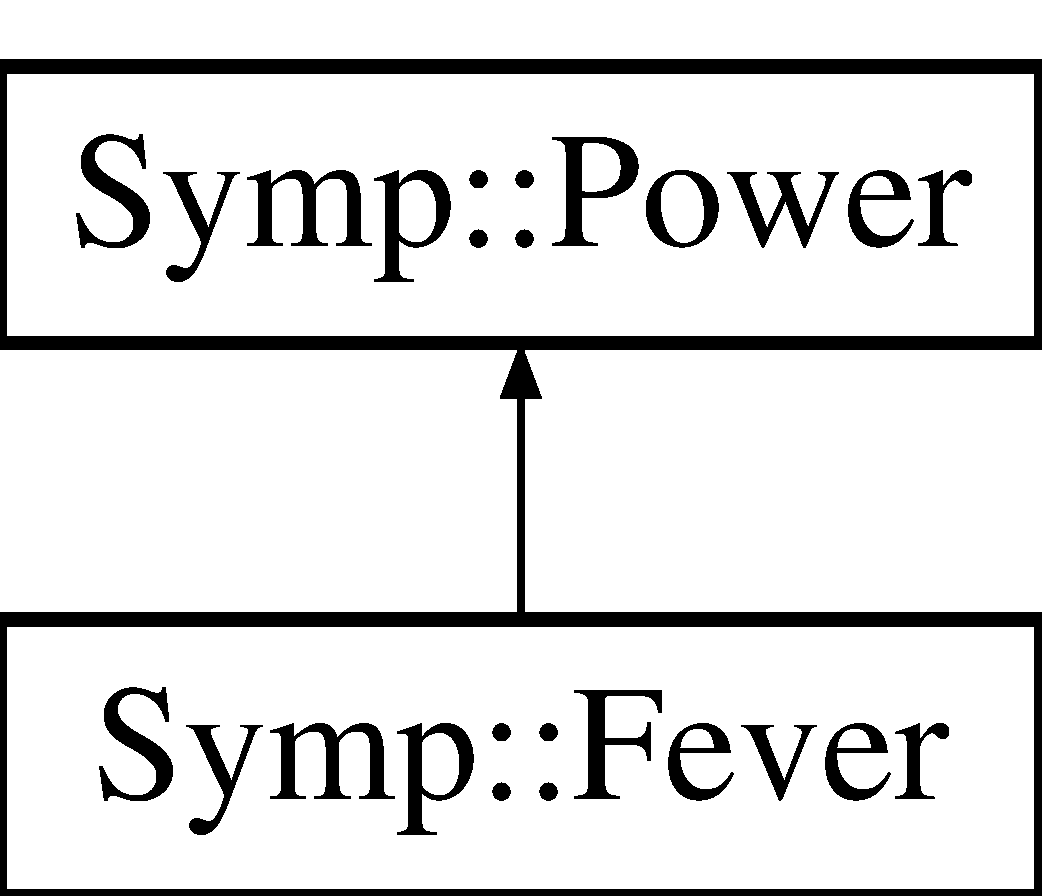
\includegraphics[height=2.000000cm]{class_symp_1_1_fever}
\end{center}
\end{figure}
\subsection*{Public Member Functions}
\begin{DoxyCompactItemize}
\item 
\hyperlink{class_symp_1_1_fever_a4458612b1d9efc07a18f8853fb9a8545}{Fever} ()
\begin{DoxyCompactList}\small\item\em \hyperlink{class_symp_1_1_fever}{Fever} class constructor. \end{DoxyCompactList}\item 
\hyperlink{class_symp_1_1_fever_a9f9a8dc3c26f4a2917a843fd8891c29b}{$\sim$\-Fever} ()
\begin{DoxyCompactList}\small\item\em \hyperlink{class_symp_1_1_fever}{Fever} class destructor. \end{DoxyCompactList}\item 
void \hyperlink{class_symp_1_1_fever_a963f59082a92165475663d3c359ffbf2}{execute} ()
\begin{DoxyCompactList}\small\item\em Implementation of the \hyperlink{class_symp_1_1_power}{Power} abstract class If the fever power is activated, this method will be called at each turn of the main loop. This method will make the character's temperature change, or not. \end{DoxyCompactList}\item 
void \hyperlink{class_symp_1_1_fever_a7dcf044b45ffc3f6ce6096ac9112d6d9}{force\-Execution} ()
\begin{DoxyCompactList}\small\item\em Force the execution of the fever. This test function is used by the developers to easely trigger the power of hot fever (temperature $>$ 0) or cold fever (temperature $<$ 0). \end{DoxyCompactList}\item 
void \hyperlink{class_symp_1_1_fever_ae3d3ca9eb9c4d449b980c59ef8c57a35}{shiver\-Background} ()
\item 
float \hyperlink{class_symp_1_1_fever_accc45e0b79d8ddebbe68e73661f35806}{get\-Current\-Temperature} () const 
\item 
const int \hyperlink{class_symp_1_1_fever_a147995a0b033255e0750602f5bd8fc89}{get\-Max\-Temperature} () const 
\item 
const int \hyperlink{class_symp_1_1_fever_a40d7fedb8a426ea2d20ccacbac33f1ea}{get\-Min\-Temperature} () const 
\item 
int \hyperlink{class_symp_1_1_fever_a3f95180cef5a902c9d140bdc4221ac63}{get\-Hot\-Range} () const 
\item 
int \hyperlink{class_symp_1_1_fever_a8ab09855d72fdf728a69ef6ae7a9b6d7}{get\-Cold\-Range} () const 
\item 
bool \hyperlink{class_symp_1_1_fever_a36d0707dec3fc130d62035ef60c5547d}{is\-In\-Hot\-Range} () const 
\item 
bool \hyperlink{class_symp_1_1_fever_ab5103968b1de44e1690323967a845b2d}{is\-In\-Cold\-Range} () const 
\item 
bool \hyperlink{class_symp_1_1_fever_aa9082a2755202c26dcd349c2e029af42}{is\-In\-Spit\-Fire\-Range} () const 
\item 
bool \hyperlink{class_symp_1_1_fever_a78178d6f9a17aa5ce3b0bcbc215c5993}{is\-In\-Shivering\-Range} () const 
\item 
float \hyperlink{class_symp_1_1_fever_ab44e2e5879501aa7168dbcfa80a7e9ff}{get\-Temperature\-Variation} () const 
\item 
bool \hyperlink{class_symp_1_1_fever_ad81c2a8bf6d614ddb6dc5b37a482f74b}{is\-In\-Hot\-Zone} () const 
\item 
bool \hyperlink{class_symp_1_1_fever_ad04a411e253dd656758dff5ae6afd536}{is\-In\-Cold\-Zone} () const 
\item 
void \hyperlink{class_symp_1_1_fever_aa2debc949529c040a93e792f7b46d0c3}{set\-Current\-Temperature} (float current\-Temperature)
\item 
void \hyperlink{class_symp_1_1_fever_af6edc8ab259b9a9070b5adc3992d44c6}{set\-Temperature\-Variation} (float temperature\-Variation)
\item 
void \hyperlink{class_symp_1_1_fever_adedf92b0758ea2e09934e58fab2b993b}{is\-In\-Hot\-Zone} (bool yes)
\item 
void \hyperlink{class_symp_1_1_fever_ac60c84733ee37b52cea9d1f99b498500}{is\-In\-Cold\-Zone} (bool yes)
\end{DoxyCompactItemize}
\subsection*{Additional Inherited Members}


\subsection{Detailed Description}


Definition at line 12 of file Fever.\-h.



\subsection{Constructor \& Destructor Documentation}
\hypertarget{class_symp_1_1_fever_a4458612b1d9efc07a18f8853fb9a8545}{\index{Symp\-::\-Fever@{Symp\-::\-Fever}!Fever@{Fever}}
\index{Fever@{Fever}!Symp::Fever@{Symp\-::\-Fever}}
\subsubsection[{Fever}]{\setlength{\rightskip}{0pt plus 5cm}Symp\-::\-Fever\-::\-Fever (
\begin{DoxyParamCaption}
{}
\end{DoxyParamCaption}
)}}\label{class_symp_1_1_fever_a4458612b1d9efc07a18f8853fb9a8545}


\hyperlink{class_symp_1_1_fever}{Fever} class constructor. 



Definition at line 7 of file Fever.\-cpp.

\hypertarget{class_symp_1_1_fever_a9f9a8dc3c26f4a2917a843fd8891c29b}{\index{Symp\-::\-Fever@{Symp\-::\-Fever}!$\sim$\-Fever@{$\sim$\-Fever}}
\index{$\sim$\-Fever@{$\sim$\-Fever}!Symp::Fever@{Symp\-::\-Fever}}
\subsubsection[{$\sim$\-Fever}]{\setlength{\rightskip}{0pt plus 5cm}Symp\-::\-Fever\-::$\sim$\-Fever (
\begin{DoxyParamCaption}
{}
\end{DoxyParamCaption}
)}}\label{class_symp_1_1_fever_a9f9a8dc3c26f4a2917a843fd8891c29b}


\hyperlink{class_symp_1_1_fever}{Fever} class destructor. 



Definition at line 19 of file Fever.\-cpp.



\subsection{Member Function Documentation}
\hypertarget{class_symp_1_1_fever_a963f59082a92165475663d3c359ffbf2}{\index{Symp\-::\-Fever@{Symp\-::\-Fever}!execute@{execute}}
\index{execute@{execute}!Symp::Fever@{Symp\-::\-Fever}}
\subsubsection[{execute}]{\setlength{\rightskip}{0pt plus 5cm}void Symp\-::\-Fever\-::execute (
\begin{DoxyParamCaption}
{}
\end{DoxyParamCaption}
)\hspace{0.3cm}{\ttfamily [virtual]}}}\label{class_symp_1_1_fever_a963f59082a92165475663d3c359ffbf2}


Implementation of the \hyperlink{class_symp_1_1_power}{Power} abstract class If the fever power is activated, this method will be called at each turn of the main loop. This method will make the character's temperature change, or not. 



Reimplemented from \hyperlink{class_symp_1_1_power_a148a017c9f01bea343d062460074eae5}{Symp\-::\-Power}.



Definition at line 23 of file Fever.\-cpp.

\hypertarget{class_symp_1_1_fever_a7dcf044b45ffc3f6ce6096ac9112d6d9}{\index{Symp\-::\-Fever@{Symp\-::\-Fever}!force\-Execution@{force\-Execution}}
\index{force\-Execution@{force\-Execution}!Symp::Fever@{Symp\-::\-Fever}}
\subsubsection[{force\-Execution}]{\setlength{\rightskip}{0pt plus 5cm}void Symp\-::\-Fever\-::force\-Execution (
\begin{DoxyParamCaption}
{}
\end{DoxyParamCaption}
)\hspace{0.3cm}{\ttfamily [virtual]}}}\label{class_symp_1_1_fever_a7dcf044b45ffc3f6ce6096ac9112d6d9}


Force the execution of the fever. This test function is used by the developers to easely trigger the power of hot fever (temperature $>$ 0) or cold fever (temperature $<$ 0). 



Reimplemented from \hyperlink{class_symp_1_1_power_acc825d941b947be435944fc4d876a118}{Symp\-::\-Power}.



Definition at line 83 of file Fever.\-cpp.

\hypertarget{class_symp_1_1_fever_a8ab09855d72fdf728a69ef6ae7a9b6d7}{\index{Symp\-::\-Fever@{Symp\-::\-Fever}!get\-Cold\-Range@{get\-Cold\-Range}}
\index{get\-Cold\-Range@{get\-Cold\-Range}!Symp::Fever@{Symp\-::\-Fever}}
\subsubsection[{get\-Cold\-Range}]{\setlength{\rightskip}{0pt plus 5cm}int Symp\-::\-Fever\-::get\-Cold\-Range (
\begin{DoxyParamCaption}
{}
\end{DoxyParamCaption}
) const\hspace{0.3cm}{\ttfamily [inline]}}}\label{class_symp_1_1_fever_a8ab09855d72fdf728a69ef6ae7a9b6d7}


Definition at line 50 of file Fever.\-h.

\hypertarget{class_symp_1_1_fever_accc45e0b79d8ddebbe68e73661f35806}{\index{Symp\-::\-Fever@{Symp\-::\-Fever}!get\-Current\-Temperature@{get\-Current\-Temperature}}
\index{get\-Current\-Temperature@{get\-Current\-Temperature}!Symp::Fever@{Symp\-::\-Fever}}
\subsubsection[{get\-Current\-Temperature}]{\setlength{\rightskip}{0pt plus 5cm}float Symp\-::\-Fever\-::get\-Current\-Temperature (
\begin{DoxyParamCaption}
{}
\end{DoxyParamCaption}
) const\hspace{0.3cm}{\ttfamily [inline]}}}\label{class_symp_1_1_fever_accc45e0b79d8ddebbe68e73661f35806}
Getters 

Definition at line 46 of file Fever.\-h.

\hypertarget{class_symp_1_1_fever_a3f95180cef5a902c9d140bdc4221ac63}{\index{Symp\-::\-Fever@{Symp\-::\-Fever}!get\-Hot\-Range@{get\-Hot\-Range}}
\index{get\-Hot\-Range@{get\-Hot\-Range}!Symp::Fever@{Symp\-::\-Fever}}
\subsubsection[{get\-Hot\-Range}]{\setlength{\rightskip}{0pt plus 5cm}int Symp\-::\-Fever\-::get\-Hot\-Range (
\begin{DoxyParamCaption}
{}
\end{DoxyParamCaption}
) const\hspace{0.3cm}{\ttfamily [inline]}}}\label{class_symp_1_1_fever_a3f95180cef5a902c9d140bdc4221ac63}


Definition at line 49 of file Fever.\-h.

\hypertarget{class_symp_1_1_fever_a147995a0b033255e0750602f5bd8fc89}{\index{Symp\-::\-Fever@{Symp\-::\-Fever}!get\-Max\-Temperature@{get\-Max\-Temperature}}
\index{get\-Max\-Temperature@{get\-Max\-Temperature}!Symp::Fever@{Symp\-::\-Fever}}
\subsubsection[{get\-Max\-Temperature}]{\setlength{\rightskip}{0pt plus 5cm}const int Symp\-::\-Fever\-::get\-Max\-Temperature (
\begin{DoxyParamCaption}
{}
\end{DoxyParamCaption}
) const\hspace{0.3cm}{\ttfamily [inline]}}}\label{class_symp_1_1_fever_a147995a0b033255e0750602f5bd8fc89}


Definition at line 47 of file Fever.\-h.

\hypertarget{class_symp_1_1_fever_a40d7fedb8a426ea2d20ccacbac33f1ea}{\index{Symp\-::\-Fever@{Symp\-::\-Fever}!get\-Min\-Temperature@{get\-Min\-Temperature}}
\index{get\-Min\-Temperature@{get\-Min\-Temperature}!Symp::Fever@{Symp\-::\-Fever}}
\subsubsection[{get\-Min\-Temperature}]{\setlength{\rightskip}{0pt plus 5cm}const int Symp\-::\-Fever\-::get\-Min\-Temperature (
\begin{DoxyParamCaption}
{}
\end{DoxyParamCaption}
) const\hspace{0.3cm}{\ttfamily [inline]}}}\label{class_symp_1_1_fever_a40d7fedb8a426ea2d20ccacbac33f1ea}


Definition at line 48 of file Fever.\-h.

\hypertarget{class_symp_1_1_fever_ab44e2e5879501aa7168dbcfa80a7e9ff}{\index{Symp\-::\-Fever@{Symp\-::\-Fever}!get\-Temperature\-Variation@{get\-Temperature\-Variation}}
\index{get\-Temperature\-Variation@{get\-Temperature\-Variation}!Symp::Fever@{Symp\-::\-Fever}}
\subsubsection[{get\-Temperature\-Variation}]{\setlength{\rightskip}{0pt plus 5cm}float Symp\-::\-Fever\-::get\-Temperature\-Variation (
\begin{DoxyParamCaption}
{}
\end{DoxyParamCaption}
) const\hspace{0.3cm}{\ttfamily [inline]}}}\label{class_symp_1_1_fever_ab44e2e5879501aa7168dbcfa80a7e9ff}


Definition at line 55 of file Fever.\-h.

\hypertarget{class_symp_1_1_fever_ab5103968b1de44e1690323967a845b2d}{\index{Symp\-::\-Fever@{Symp\-::\-Fever}!is\-In\-Cold\-Range@{is\-In\-Cold\-Range}}
\index{is\-In\-Cold\-Range@{is\-In\-Cold\-Range}!Symp::Fever@{Symp\-::\-Fever}}
\subsubsection[{is\-In\-Cold\-Range}]{\setlength{\rightskip}{0pt plus 5cm}bool Symp\-::\-Fever\-::is\-In\-Cold\-Range (
\begin{DoxyParamCaption}
{}
\end{DoxyParamCaption}
) const\hspace{0.3cm}{\ttfamily [inline]}}}\label{class_symp_1_1_fever_ab5103968b1de44e1690323967a845b2d}


Definition at line 52 of file Fever.\-h.

\hypertarget{class_symp_1_1_fever_ad04a411e253dd656758dff5ae6afd536}{\index{Symp\-::\-Fever@{Symp\-::\-Fever}!is\-In\-Cold\-Zone@{is\-In\-Cold\-Zone}}
\index{is\-In\-Cold\-Zone@{is\-In\-Cold\-Zone}!Symp::Fever@{Symp\-::\-Fever}}
\subsubsection[{is\-In\-Cold\-Zone}]{\setlength{\rightskip}{0pt plus 5cm}bool Symp\-::\-Fever\-::is\-In\-Cold\-Zone (
\begin{DoxyParamCaption}
{}
\end{DoxyParamCaption}
) const\hspace{0.3cm}{\ttfamily [inline]}}}\label{class_symp_1_1_fever_ad04a411e253dd656758dff5ae6afd536}


Definition at line 57 of file Fever.\-h.

\hypertarget{class_symp_1_1_fever_ac60c84733ee37b52cea9d1f99b498500}{\index{Symp\-::\-Fever@{Symp\-::\-Fever}!is\-In\-Cold\-Zone@{is\-In\-Cold\-Zone}}
\index{is\-In\-Cold\-Zone@{is\-In\-Cold\-Zone}!Symp::Fever@{Symp\-::\-Fever}}
\subsubsection[{is\-In\-Cold\-Zone}]{\setlength{\rightskip}{0pt plus 5cm}void Symp\-::\-Fever\-::is\-In\-Cold\-Zone (
\begin{DoxyParamCaption}
\item[{bool}]{yes}
\end{DoxyParamCaption}
)\hspace{0.3cm}{\ttfamily [inline]}}}\label{class_symp_1_1_fever_ac60c84733ee37b52cea9d1f99b498500}


Definition at line 68 of file Fever.\-h.

\hypertarget{class_symp_1_1_fever_a36d0707dec3fc130d62035ef60c5547d}{\index{Symp\-::\-Fever@{Symp\-::\-Fever}!is\-In\-Hot\-Range@{is\-In\-Hot\-Range}}
\index{is\-In\-Hot\-Range@{is\-In\-Hot\-Range}!Symp::Fever@{Symp\-::\-Fever}}
\subsubsection[{is\-In\-Hot\-Range}]{\setlength{\rightskip}{0pt plus 5cm}bool Symp\-::\-Fever\-::is\-In\-Hot\-Range (
\begin{DoxyParamCaption}
{}
\end{DoxyParamCaption}
) const\hspace{0.3cm}{\ttfamily [inline]}}}\label{class_symp_1_1_fever_a36d0707dec3fc130d62035ef60c5547d}


Definition at line 51 of file Fever.\-h.

\hypertarget{class_symp_1_1_fever_ad81c2a8bf6d614ddb6dc5b37a482f74b}{\index{Symp\-::\-Fever@{Symp\-::\-Fever}!is\-In\-Hot\-Zone@{is\-In\-Hot\-Zone}}
\index{is\-In\-Hot\-Zone@{is\-In\-Hot\-Zone}!Symp::Fever@{Symp\-::\-Fever}}
\subsubsection[{is\-In\-Hot\-Zone}]{\setlength{\rightskip}{0pt plus 5cm}bool Symp\-::\-Fever\-::is\-In\-Hot\-Zone (
\begin{DoxyParamCaption}
{}
\end{DoxyParamCaption}
) const\hspace{0.3cm}{\ttfamily [inline]}}}\label{class_symp_1_1_fever_ad81c2a8bf6d614ddb6dc5b37a482f74b}


Definition at line 56 of file Fever.\-h.

\hypertarget{class_symp_1_1_fever_adedf92b0758ea2e09934e58fab2b993b}{\index{Symp\-::\-Fever@{Symp\-::\-Fever}!is\-In\-Hot\-Zone@{is\-In\-Hot\-Zone}}
\index{is\-In\-Hot\-Zone@{is\-In\-Hot\-Zone}!Symp::Fever@{Symp\-::\-Fever}}
\subsubsection[{is\-In\-Hot\-Zone}]{\setlength{\rightskip}{0pt plus 5cm}void Symp\-::\-Fever\-::is\-In\-Hot\-Zone (
\begin{DoxyParamCaption}
\item[{bool}]{yes}
\end{DoxyParamCaption}
)\hspace{0.3cm}{\ttfamily [inline]}}}\label{class_symp_1_1_fever_adedf92b0758ea2e09934e58fab2b993b}


Definition at line 64 of file Fever.\-h.

\hypertarget{class_symp_1_1_fever_a78178d6f9a17aa5ce3b0bcbc215c5993}{\index{Symp\-::\-Fever@{Symp\-::\-Fever}!is\-In\-Shivering\-Range@{is\-In\-Shivering\-Range}}
\index{is\-In\-Shivering\-Range@{is\-In\-Shivering\-Range}!Symp::Fever@{Symp\-::\-Fever}}
\subsubsection[{is\-In\-Shivering\-Range}]{\setlength{\rightskip}{0pt plus 5cm}bool Symp\-::\-Fever\-::is\-In\-Shivering\-Range (
\begin{DoxyParamCaption}
{}
\end{DoxyParamCaption}
) const\hspace{0.3cm}{\ttfamily [inline]}}}\label{class_symp_1_1_fever_a78178d6f9a17aa5ce3b0bcbc215c5993}


Definition at line 54 of file Fever.\-h.

\hypertarget{class_symp_1_1_fever_aa9082a2755202c26dcd349c2e029af42}{\index{Symp\-::\-Fever@{Symp\-::\-Fever}!is\-In\-Spit\-Fire\-Range@{is\-In\-Spit\-Fire\-Range}}
\index{is\-In\-Spit\-Fire\-Range@{is\-In\-Spit\-Fire\-Range}!Symp::Fever@{Symp\-::\-Fever}}
\subsubsection[{is\-In\-Spit\-Fire\-Range}]{\setlength{\rightskip}{0pt plus 5cm}bool Symp\-::\-Fever\-::is\-In\-Spit\-Fire\-Range (
\begin{DoxyParamCaption}
{}
\end{DoxyParamCaption}
) const\hspace{0.3cm}{\ttfamily [inline]}}}\label{class_symp_1_1_fever_aa9082a2755202c26dcd349c2e029af42}


Definition at line 53 of file Fever.\-h.

\hypertarget{class_symp_1_1_fever_aa2debc949529c040a93e792f7b46d0c3}{\index{Symp\-::\-Fever@{Symp\-::\-Fever}!set\-Current\-Temperature@{set\-Current\-Temperature}}
\index{set\-Current\-Temperature@{set\-Current\-Temperature}!Symp::Fever@{Symp\-::\-Fever}}
\subsubsection[{set\-Current\-Temperature}]{\setlength{\rightskip}{0pt plus 5cm}void Symp\-::\-Fever\-::set\-Current\-Temperature (
\begin{DoxyParamCaption}
\item[{float}]{current\-Temperature}
\end{DoxyParamCaption}
)\hspace{0.3cm}{\ttfamily [inline]}}}\label{class_symp_1_1_fever_aa2debc949529c040a93e792f7b46d0c3}
Setters 

Definition at line 62 of file Fever.\-h.

\hypertarget{class_symp_1_1_fever_af6edc8ab259b9a9070b5adc3992d44c6}{\index{Symp\-::\-Fever@{Symp\-::\-Fever}!set\-Temperature\-Variation@{set\-Temperature\-Variation}}
\index{set\-Temperature\-Variation@{set\-Temperature\-Variation}!Symp::Fever@{Symp\-::\-Fever}}
\subsubsection[{set\-Temperature\-Variation}]{\setlength{\rightskip}{0pt plus 5cm}void Symp\-::\-Fever\-::set\-Temperature\-Variation (
\begin{DoxyParamCaption}
\item[{float}]{temperature\-Variation}
\end{DoxyParamCaption}
)\hspace{0.3cm}{\ttfamily [inline]}}}\label{class_symp_1_1_fever_af6edc8ab259b9a9070b5adc3992d44c6}


Definition at line 63 of file Fever.\-h.

\hypertarget{class_symp_1_1_fever_ae3d3ca9eb9c4d449b980c59ef8c57a35}{\index{Symp\-::\-Fever@{Symp\-::\-Fever}!shiver\-Background@{shiver\-Background}}
\index{shiver\-Background@{shiver\-Background}!Symp::Fever@{Symp\-::\-Fever}}
\subsubsection[{shiver\-Background}]{\setlength{\rightskip}{0pt plus 5cm}void Symp\-::\-Fever\-::shiver\-Background (
\begin{DoxyParamCaption}
{}
\end{DoxyParamCaption}
)}}\label{class_symp_1_1_fever_ae3d3ca9eb9c4d449b980c59ef8c57a35}


Definition at line 94 of file Fever.\-cpp.



The documentation for this class was generated from the following files\-:\begin{DoxyCompactItemize}
\item 
/home/cecilia/\-Documents/\-Symptogen/src/power/\hyperlink{_fever_8h}{Fever.\-h}\item 
/home/cecilia/\-Documents/\-Symptogen/src/power/\hyperlink{_fever_8cpp}{Fever.\-cpp}\end{DoxyCompactItemize}

\hypertarget{class_symp_1_1_game_manager}{\section{Symp\-:\-:Game\-Manager Class Reference}
\label{class_symp_1_1_game_manager}\index{Symp\-::\-Game\-Manager@{Symp\-::\-Game\-Manager}}
}


{\ttfamily \#include $<$Game\-Manager.\-h$>$}

Inheritance diagram for Symp\-:\-:Game\-Manager\-:\begin{figure}[H]
\begin{center}
\leavevmode
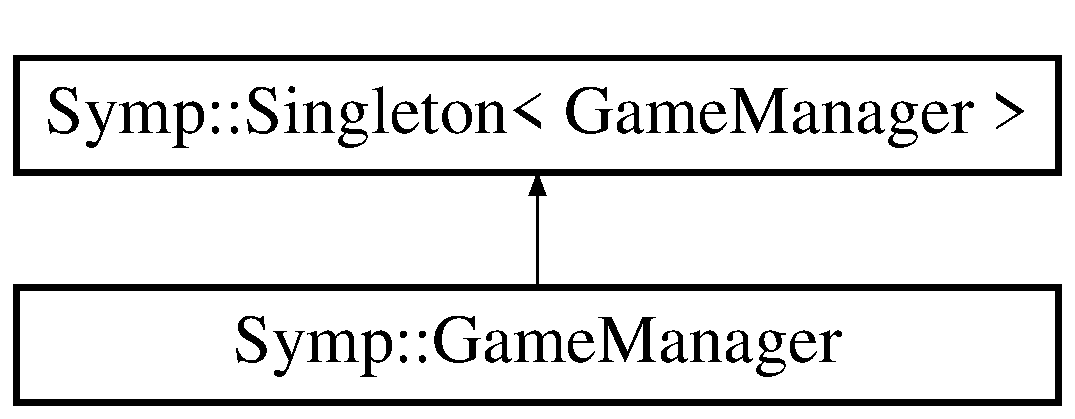
\includegraphics[height=2.000000cm]{class_symp_1_1_game_manager}
\end{center}
\end{figure}
\subsection*{Public Member Functions}
\begin{DoxyCompactItemize}
\item 
void \hyperlink{class_symp_1_1_game_manager_a997c17dcac4e9454a9ed7e14f0dd4ca9}{clear} ()
\begin{DoxyCompactList}\small\item\em Clear the game entities and attributes for displaying the main menu. \end{DoxyCompactList}\item 
void \hyperlink{class_symp_1_1_game_manager_a966aa77267116aa3d7056b5e48278e17}{start\-Main\-Loop} ()
\begin{DoxyCompactList}\small\item\em The main loop of the game responsible the application to run. \end{DoxyCompactList}\item 
void \hyperlink{class_symp_1_1_game_manager_a3036c6f74cf03eed27cef74e93ff502b}{update\-Game} ()
\begin{DoxyCompactList}\small\item\em Update the game part of the application each loop. \end{DoxyCompactList}\item 
void \hyperlink{class_symp_1_1_game_manager_a53eae391ee3ea958e26d60b51516c770}{update\-Menu} ()
\begin{DoxyCompactList}\small\item\em Update the menu part of the application each loop. \end{DoxyCompactList}\item 
void \hyperlink{class_symp_1_1_game_manager_a6bde65ad61b89c3d86ecfc53e0b89dfd}{switch\-To\-Game} ()
\begin{DoxyCompactList}\small\item\em Displays the game when it needs to be This function displays the game, usually called from a menu. \end{DoxyCompactList}\item 
void \hyperlink{class_symp_1_1_game_manager_a7232828cd96d0c7fe947406f73426a9e}{switch\-To\-Menu} ()
\begin{DoxyCompactList}\small\item\em Displays the menus when it needs to be This function displays wether the main menu, or the \hyperlink{class_symp_1_1_pause_menu}{Pause\-Menu}. This function can be called in game for displaying again the main menus, in this case, the \#\-Game\-Manager needs to be cleared using the \hyperlink{class_symp_1_1_game_manager_a997c17dcac4e9454a9ed7e14f0dd4ca9}{clear()} function. To display the game, see \hyperlink{class_symp_1_1_game_manager_a6bde65ad61b89c3d86ecfc53e0b89dfd}{switch\-To\-Game()}. \end{DoxyCompactList}\item 
void \hyperlink{class_symp_1_1_game_manager_a330de72544980faa5889c81c7d05bec5}{load\-Level} (const char $\ast$map\-File)
\begin{DoxyCompactList}\small\item\em Delete all existing entities and powers, and load the map\-File by calling the parser. \end{DoxyCompactList}\item 
void \hyperlink{class_symp_1_1_game_manager_a1c0d73555fbec1f38e6be3f1f838f8ac}{load\-Current\-Level} ()
\item 
void \hyperlink{class_symp_1_1_game_manager_a4916acefa261d4db81bc1dd26cb2b403}{debug\-Physical\-Entities} ()
\begin{DoxyCompactList}\small\item\em Debug tool, useful to display hitboxes and center of all physical entities. \end{DoxyCompactList}\item 
void \hyperlink{class_symp_1_1_game_manager_a448082eae851a482e66df7b989f0eea9}{debug\-Render\-Entities} ()
\begin{DoxyCompactList}\small\item\em Debug tool, useful to display the size and the center of all render entities. \end{DoxyCompactList}\item 
void \hyperlink{class_symp_1_1_game_manager_a3498f818c58050eae82f06cd4e281874}{load\-Physics} ()
\begin{DoxyCompactList}\small\item\em Reload physical value at the beginning or after death and reload level. \end{DoxyCompactList}\item 
void \hyperlink{class_symp_1_1_game_manager_a37bd929c492f811d45affc348b5a96dd}{reload\-Level} ()
\item 
void \hyperlink{class_symp_1_1_game_manager_ae50df7b7d6bbc9b3ae4b5881e5a38724}{create\-Kinematic} ()
\item 
\hyperlink{class_symp_1_1_window}{Window} $\ast$ \hyperlink{class_symp_1_1_game_manager_aa415fa93a61f52538c55513ab84b2148}{get\-Window} () const 
\item 
\hyperlink{class_symp_1_1_render}{Render} $\ast$ \hyperlink{class_symp_1_1_game_manager_a95eba8af1a70bd697b2d14aa50bd5554}{get\-Render} () const 
\item 
bool \hyperlink{class_symp_1_1_game_manager_a251b46e6c4c221119e54f66c93e70ce0}{get\-Is\-In\-Game} () const 
\item 
int \hyperlink{class_symp_1_1_game_manager_ac1255f7ce1f67eb67a39197b86d17d23}{get\-Is\-Player\-Noob} () const 
\item 
void \hyperlink{class_symp_1_1_game_manager_a8deb8d3ed654d6651ec3b7ab57c8a1bd}{set\-Is\-Player\-Dead} (bool value)
\item 
void \hyperlink{class_symp_1_1_game_manager_a29a45f9f3c6a75f0801b7804f6c6876a}{set\-Is\-Player\-Noob} (int value)
\end{DoxyCompactItemize}
\subsection*{Friends}
\begin{DoxyCompactItemize}
\item 
class \hyperlink{class_symp_1_1_game_manager_aea7e15ea69de786a42266b0f5cdd4a9c}{Singleton$<$ Game\-Manager $>$}
\end{DoxyCompactItemize}
\subsection*{Additional Inherited Members}


\subsection{Detailed Description}
Manages the loop of the game. It has to be a singleton. It has the role of a dispatcher, distributing tasks to other objects (\hyperlink{class_symp_1_1_render}{Render}, all Parsers...). It provides tools to \-:
\begin{DoxyItemize}
\item Manage main loop
\item Switch to menu
\item Switch to game 
\end{DoxyItemize}

Definition at line 31 of file Game\-Manager.\-h.



\subsection{Member Function Documentation}
\hypertarget{class_symp_1_1_game_manager_a997c17dcac4e9454a9ed7e14f0dd4ca9}{\index{Symp\-::\-Game\-Manager@{Symp\-::\-Game\-Manager}!clear@{clear}}
\index{clear@{clear}!Symp::GameManager@{Symp\-::\-Game\-Manager}}
\subsubsection[{clear}]{\setlength{\rightskip}{0pt plus 5cm}void Symp\-::\-Game\-Manager\-::clear (
\begin{DoxyParamCaption}
{}
\end{DoxyParamCaption}
)}}\label{class_symp_1_1_game_manager_a997c17dcac4e9454a9ed7e14f0dd4ca9}


Clear the game entities and attributes for displaying the main menu. 

\begin{DoxySeeAlso}{See Also}
\hyperlink{class_symp_1_1_menu_manager}{Menu\-Manager} 

\hyperlink{class_symp_1_1_entity_manager}{Entity\-Manager} 

Level\-Manager 

\hyperlink{class_symp_1_1_game_manager_a53eae391ee3ea958e26d60b51516c770}{update\-Menu()} 

Game\-Manager() 

$\sim$\-Game\-Manager() 
\end{DoxySeeAlso}


Definition at line 94 of file Game\-Manager.\-cpp.

\hypertarget{class_symp_1_1_game_manager_ae50df7b7d6bbc9b3ae4b5881e5a38724}{\index{Symp\-::\-Game\-Manager@{Symp\-::\-Game\-Manager}!create\-Kinematic@{create\-Kinematic}}
\index{create\-Kinematic@{create\-Kinematic}!Symp::GameManager@{Symp\-::\-Game\-Manager}}
\subsubsection[{create\-Kinematic}]{\setlength{\rightskip}{0pt plus 5cm}void Symp\-::\-Game\-Manager\-::create\-Kinematic (
\begin{DoxyParamCaption}
{}
\end{DoxyParamCaption}
)}}\label{class_symp_1_1_game_manager_ae50df7b7d6bbc9b3ae4b5881e5a38724}


Definition at line 122 of file Game\-Manager.\-cpp.

\hypertarget{class_symp_1_1_game_manager_a4916acefa261d4db81bc1dd26cb2b403}{\index{Symp\-::\-Game\-Manager@{Symp\-::\-Game\-Manager}!debug\-Physical\-Entities@{debug\-Physical\-Entities}}
\index{debug\-Physical\-Entities@{debug\-Physical\-Entities}!Symp::GameManager@{Symp\-::\-Game\-Manager}}
\subsubsection[{debug\-Physical\-Entities}]{\setlength{\rightskip}{0pt plus 5cm}void Symp\-::\-Game\-Manager\-::debug\-Physical\-Entities (
\begin{DoxyParamCaption}
{}
\end{DoxyParamCaption}
)}}\label{class_symp_1_1_game_manager_a4916acefa261d4db81bc1dd26cb2b403}


Debug tool, useful to display hitboxes and center of all physical entities. 

\begin{DoxySeeAlso}{See Also}
\hyperlink{class_symp_1_1_entity_manager}{Entity\-Manager} 
\end{DoxySeeAlso}


Definition at line 671 of file Game\-Manager.\-cpp.

\hypertarget{class_symp_1_1_game_manager_a448082eae851a482e66df7b989f0eea9}{\index{Symp\-::\-Game\-Manager@{Symp\-::\-Game\-Manager}!debug\-Render\-Entities@{debug\-Render\-Entities}}
\index{debug\-Render\-Entities@{debug\-Render\-Entities}!Symp::GameManager@{Symp\-::\-Game\-Manager}}
\subsubsection[{debug\-Render\-Entities}]{\setlength{\rightskip}{0pt plus 5cm}void Symp\-::\-Game\-Manager\-::debug\-Render\-Entities (
\begin{DoxyParamCaption}
{}
\end{DoxyParamCaption}
)}}\label{class_symp_1_1_game_manager_a448082eae851a482e66df7b989f0eea9}


Debug tool, useful to display the size and the center of all render entities. 

\begin{DoxySeeAlso}{See Also}
\hyperlink{class_symp_1_1_entity_manager}{Entity\-Manager} 
\end{DoxySeeAlso}


Definition at line 724 of file Game\-Manager.\-cpp.

\hypertarget{class_symp_1_1_game_manager_a251b46e6c4c221119e54f66c93e70ce0}{\index{Symp\-::\-Game\-Manager@{Symp\-::\-Game\-Manager}!get\-Is\-In\-Game@{get\-Is\-In\-Game}}
\index{get\-Is\-In\-Game@{get\-Is\-In\-Game}!Symp::GameManager@{Symp\-::\-Game\-Manager}}
\subsubsection[{get\-Is\-In\-Game}]{\setlength{\rightskip}{0pt plus 5cm}bool Symp\-::\-Game\-Manager\-::get\-Is\-In\-Game (
\begin{DoxyParamCaption}
{}
\end{DoxyParamCaption}
) const\hspace{0.3cm}{\ttfamily [inline]}}}\label{class_symp_1_1_game_manager_a251b46e6c4c221119e54f66c93e70ce0}


Definition at line 146 of file Game\-Manager.\-h.

\hypertarget{class_symp_1_1_game_manager_ac1255f7ce1f67eb67a39197b86d17d23}{\index{Symp\-::\-Game\-Manager@{Symp\-::\-Game\-Manager}!get\-Is\-Player\-Noob@{get\-Is\-Player\-Noob}}
\index{get\-Is\-Player\-Noob@{get\-Is\-Player\-Noob}!Symp::GameManager@{Symp\-::\-Game\-Manager}}
\subsubsection[{get\-Is\-Player\-Noob}]{\setlength{\rightskip}{0pt plus 5cm}int Symp\-::\-Game\-Manager\-::get\-Is\-Player\-Noob (
\begin{DoxyParamCaption}
{}
\end{DoxyParamCaption}
) const\hspace{0.3cm}{\ttfamily [inline]}}}\label{class_symp_1_1_game_manager_ac1255f7ce1f67eb67a39197b86d17d23}


Definition at line 147 of file Game\-Manager.\-h.

\hypertarget{class_symp_1_1_game_manager_a95eba8af1a70bd697b2d14aa50bd5554}{\index{Symp\-::\-Game\-Manager@{Symp\-::\-Game\-Manager}!get\-Render@{get\-Render}}
\index{get\-Render@{get\-Render}!Symp::GameManager@{Symp\-::\-Game\-Manager}}
\subsubsection[{get\-Render}]{\setlength{\rightskip}{0pt plus 5cm}{\bf Render}$\ast$ Symp\-::\-Game\-Manager\-::get\-Render (
\begin{DoxyParamCaption}
{}
\end{DoxyParamCaption}
) const\hspace{0.3cm}{\ttfamily [inline]}}}\label{class_symp_1_1_game_manager_a95eba8af1a70bd697b2d14aa50bd5554}


Definition at line 145 of file Game\-Manager.\-h.

\hypertarget{class_symp_1_1_game_manager_aa415fa93a61f52538c55513ab84b2148}{\index{Symp\-::\-Game\-Manager@{Symp\-::\-Game\-Manager}!get\-Window@{get\-Window}}
\index{get\-Window@{get\-Window}!Symp::GameManager@{Symp\-::\-Game\-Manager}}
\subsubsection[{get\-Window}]{\setlength{\rightskip}{0pt plus 5cm}{\bf Window}$\ast$ Symp\-::\-Game\-Manager\-::get\-Window (
\begin{DoxyParamCaption}
{}
\end{DoxyParamCaption}
) const\hspace{0.3cm}{\ttfamily [inline]}}}\label{class_symp_1_1_game_manager_aa415fa93a61f52538c55513ab84b2148}
Getters 

Definition at line 144 of file Game\-Manager.\-h.

\hypertarget{class_symp_1_1_game_manager_a1c0d73555fbec1f38e6be3f1f838f8ac}{\index{Symp\-::\-Game\-Manager@{Symp\-::\-Game\-Manager}!load\-Current\-Level@{load\-Current\-Level}}
\index{load\-Current\-Level@{load\-Current\-Level}!Symp::GameManager@{Symp\-::\-Game\-Manager}}
\subsubsection[{load\-Current\-Level}]{\setlength{\rightskip}{0pt plus 5cm}void Symp\-::\-Game\-Manager\-::load\-Current\-Level (
\begin{DoxyParamCaption}
{}
\end{DoxyParamCaption}
)\hspace{0.3cm}{\ttfamily [inline]}}}\label{class_symp_1_1_game_manager_a1c0d73555fbec1f38e6be3f1f838f8ac}


Definition at line 115 of file Game\-Manager.\-h.

\hypertarget{class_symp_1_1_game_manager_a330de72544980faa5889c81c7d05bec5}{\index{Symp\-::\-Game\-Manager@{Symp\-::\-Game\-Manager}!load\-Level@{load\-Level}}
\index{load\-Level@{load\-Level}!Symp::GameManager@{Symp\-::\-Game\-Manager}}
\subsubsection[{load\-Level}]{\setlength{\rightskip}{0pt plus 5cm}void Symp\-::\-Game\-Manager\-::load\-Level (
\begin{DoxyParamCaption}
\item[{const char $\ast$}]{map\-File}
\end{DoxyParamCaption}
)}}\label{class_symp_1_1_game_manager_a330de72544980faa5889c81c7d05bec5}


Delete all existing entities and powers, and load the map\-File by calling the parser. 

\begin{DoxySeeAlso}{See Also}
Parser 
\end{DoxySeeAlso}


Definition at line 621 of file Game\-Manager.\-cpp.

\hypertarget{class_symp_1_1_game_manager_a3498f818c58050eae82f06cd4e281874}{\index{Symp\-::\-Game\-Manager@{Symp\-::\-Game\-Manager}!load\-Physics@{load\-Physics}}
\index{load\-Physics@{load\-Physics}!Symp::GameManager@{Symp\-::\-Game\-Manager}}
\subsubsection[{load\-Physics}]{\setlength{\rightskip}{0pt plus 5cm}void Symp\-::\-Game\-Manager\-::load\-Physics (
\begin{DoxyParamCaption}
{}
\end{DoxyParamCaption}
)}}\label{class_symp_1_1_game_manager_a3498f818c58050eae82f06cd4e281874}


Reload physical value at the beginning or after death and reload level. 



Definition at line 754 of file Game\-Manager.\-cpp.

\hypertarget{class_symp_1_1_game_manager_a37bd929c492f811d45affc348b5a96dd}{\index{Symp\-::\-Game\-Manager@{Symp\-::\-Game\-Manager}!reload\-Level@{reload\-Level}}
\index{reload\-Level@{reload\-Level}!Symp::GameManager@{Symp\-::\-Game\-Manager}}
\subsubsection[{reload\-Level}]{\setlength{\rightskip}{0pt plus 5cm}void Symp\-::\-Game\-Manager\-::reload\-Level (
\begin{DoxyParamCaption}
{}
\end{DoxyParamCaption}
)}}\label{class_symp_1_1_game_manager_a37bd929c492f811d45affc348b5a96dd}


Definition at line 665 of file Game\-Manager.\-cpp.

\hypertarget{class_symp_1_1_game_manager_a8deb8d3ed654d6651ec3b7ab57c8a1bd}{\index{Symp\-::\-Game\-Manager@{Symp\-::\-Game\-Manager}!set\-Is\-Player\-Dead@{set\-Is\-Player\-Dead}}
\index{set\-Is\-Player\-Dead@{set\-Is\-Player\-Dead}!Symp::GameManager@{Symp\-::\-Game\-Manager}}
\subsubsection[{set\-Is\-Player\-Dead}]{\setlength{\rightskip}{0pt plus 5cm}void Symp\-::\-Game\-Manager\-::set\-Is\-Player\-Dead (
\begin{DoxyParamCaption}
\item[{bool}]{value}
\end{DoxyParamCaption}
)\hspace{0.3cm}{\ttfamily [inline]}}}\label{class_symp_1_1_game_manager_a8deb8d3ed654d6651ec3b7ab57c8a1bd}
Setters 

Definition at line 152 of file Game\-Manager.\-h.

\hypertarget{class_symp_1_1_game_manager_a29a45f9f3c6a75f0801b7804f6c6876a}{\index{Symp\-::\-Game\-Manager@{Symp\-::\-Game\-Manager}!set\-Is\-Player\-Noob@{set\-Is\-Player\-Noob}}
\index{set\-Is\-Player\-Noob@{set\-Is\-Player\-Noob}!Symp::GameManager@{Symp\-::\-Game\-Manager}}
\subsubsection[{set\-Is\-Player\-Noob}]{\setlength{\rightskip}{0pt plus 5cm}void Symp\-::\-Game\-Manager\-::set\-Is\-Player\-Noob (
\begin{DoxyParamCaption}
\item[{int}]{value}
\end{DoxyParamCaption}
)\hspace{0.3cm}{\ttfamily [inline]}}}\label{class_symp_1_1_game_manager_a29a45f9f3c6a75f0801b7804f6c6876a}


Definition at line 153 of file Game\-Manager.\-h.

\hypertarget{class_symp_1_1_game_manager_a966aa77267116aa3d7056b5e48278e17}{\index{Symp\-::\-Game\-Manager@{Symp\-::\-Game\-Manager}!start\-Main\-Loop@{start\-Main\-Loop}}
\index{start\-Main\-Loop@{start\-Main\-Loop}!Symp::GameManager@{Symp\-::\-Game\-Manager}}
\subsubsection[{start\-Main\-Loop}]{\setlength{\rightskip}{0pt plus 5cm}void Symp\-::\-Game\-Manager\-::start\-Main\-Loop (
\begin{DoxyParamCaption}
{}
\end{DoxyParamCaption}
)}}\label{class_symp_1_1_game_manager_a966aa77267116aa3d7056b5e48278e17}


The main loop of the game responsible the application to run. 

\begin{DoxySeeAlso}{See Also}
\hyperlink{class_symp_1_1_game_manager_a53eae391ee3ea958e26d60b51516c770}{update\-Menu()} 

\hyperlink{class_symp_1_1_game_manager_a3036c6f74cf03eed27cef74e93ff502b}{update\-Game()} 

\hyperlink{class_symp_1_1_game_manager_a6bde65ad61b89c3d86ecfc53e0b89dfd}{switch\-To\-Game()} 

\hyperlink{class_symp_1_1_game_manager_a7232828cd96d0c7fe947406f73426a9e}{switch\-To\-Menu()} 

Game\-Manager() 

$\sim$\-Game\-Manager() 
\end{DoxySeeAlso}


Definition at line 106 of file Game\-Manager.\-cpp.

\hypertarget{class_symp_1_1_game_manager_a6bde65ad61b89c3d86ecfc53e0b89dfd}{\index{Symp\-::\-Game\-Manager@{Symp\-::\-Game\-Manager}!switch\-To\-Game@{switch\-To\-Game}}
\index{switch\-To\-Game@{switch\-To\-Game}!Symp::GameManager@{Symp\-::\-Game\-Manager}}
\subsubsection[{switch\-To\-Game}]{\setlength{\rightskip}{0pt plus 5cm}void Symp\-::\-Game\-Manager\-::switch\-To\-Game (
\begin{DoxyParamCaption}
{}
\end{DoxyParamCaption}
)}}\label{class_symp_1_1_game_manager_a6bde65ad61b89c3d86ecfc53e0b89dfd}


Displays the game when it needs to be This function displays the game, usually called from a menu. 

\begin{DoxySeeAlso}{See Also}
\hyperlink{class_symp_1_1_menu_manager}{Menu\-Manager} 

\hyperlink{class_symp_1_1_game_manager_a3036c6f74cf03eed27cef74e93ff502b}{update\-Game()} 

\hyperlink{class_symp_1_1_game_manager_a7232828cd96d0c7fe947406f73426a9e}{switch\-To\-Menu()} 

Game\-Manager() 

$\sim$\-Game\-Manager() 
\end{DoxySeeAlso}


Definition at line 491 of file Game\-Manager.\-cpp.

\hypertarget{class_symp_1_1_game_manager_a7232828cd96d0c7fe947406f73426a9e}{\index{Symp\-::\-Game\-Manager@{Symp\-::\-Game\-Manager}!switch\-To\-Menu@{switch\-To\-Menu}}
\index{switch\-To\-Menu@{switch\-To\-Menu}!Symp::GameManager@{Symp\-::\-Game\-Manager}}
\subsubsection[{switch\-To\-Menu}]{\setlength{\rightskip}{0pt plus 5cm}void Symp\-::\-Game\-Manager\-::switch\-To\-Menu (
\begin{DoxyParamCaption}
{}
\end{DoxyParamCaption}
)}}\label{class_symp_1_1_game_manager_a7232828cd96d0c7fe947406f73426a9e}


Displays the menus when it needs to be This function displays wether the main menu, or the \hyperlink{class_symp_1_1_pause_menu}{Pause\-Menu}. This function can be called in game for displaying again the main menus, in this case, the \#\-Game\-Manager needs to be cleared using the \hyperlink{class_symp_1_1_game_manager_a997c17dcac4e9454a9ed7e14f0dd4ca9}{clear()} function. To display the game, see \hyperlink{class_symp_1_1_game_manager_a6bde65ad61b89c3d86ecfc53e0b89dfd}{switch\-To\-Game()}. 

\begin{DoxySeeAlso}{See Also}
\hyperlink{class_symp_1_1_menu_manager}{Menu\-Manager} 

\hyperlink{class_symp_1_1_game_manager_a53eae391ee3ea958e26d60b51516c770}{update\-Menu()} 

\hyperlink{class_symp_1_1_game_manager_a6bde65ad61b89c3d86ecfc53e0b89dfd}{switch\-To\-Game()} 

Game\-Manager() 

$\sim$\-Game\-Manager() 
\end{DoxySeeAlso}


Definition at line 585 of file Game\-Manager.\-cpp.

\hypertarget{class_symp_1_1_game_manager_a3036c6f74cf03eed27cef74e93ff502b}{\index{Symp\-::\-Game\-Manager@{Symp\-::\-Game\-Manager}!update\-Game@{update\-Game}}
\index{update\-Game@{update\-Game}!Symp::GameManager@{Symp\-::\-Game\-Manager}}
\subsubsection[{update\-Game}]{\setlength{\rightskip}{0pt plus 5cm}void Symp\-::\-Game\-Manager\-::update\-Game (
\begin{DoxyParamCaption}
{}
\end{DoxyParamCaption}
)}}\label{class_symp_1_1_game_manager_a3036c6f74cf03eed27cef74e93ff502b}


Update the game part of the application each loop. 

\begin{DoxySeeAlso}{See Also}
\hyperlink{class_symp_1_1_game_manager_a53eae391ee3ea958e26d60b51516c770}{update\-Menu()} 

\hyperlink{class_symp_1_1_input_manager}{Input\-Manager} 

\hyperlink{class_symp_1_1_game_manager_a6bde65ad61b89c3d86ecfc53e0b89dfd}{switch\-To\-Game()} 

\hyperlink{class_symp_1_1_game_manager_a7232828cd96d0c7fe947406f73426a9e}{switch\-To\-Menu()} 

\hyperlink{class_symp_1_1_entity_manager}{Entity\-Manager} 

Game\-Manager() 

$\sim$\-Game\-Manager() 
\end{DoxySeeAlso}


Definition at line 186 of file Game\-Manager.\-cpp.

\hypertarget{class_symp_1_1_game_manager_a53eae391ee3ea958e26d60b51516c770}{\index{Symp\-::\-Game\-Manager@{Symp\-::\-Game\-Manager}!update\-Menu@{update\-Menu}}
\index{update\-Menu@{update\-Menu}!Symp::GameManager@{Symp\-::\-Game\-Manager}}
\subsubsection[{update\-Menu}]{\setlength{\rightskip}{0pt plus 5cm}void Symp\-::\-Game\-Manager\-::update\-Menu (
\begin{DoxyParamCaption}
{}
\end{DoxyParamCaption}
)}}\label{class_symp_1_1_game_manager_a53eae391ee3ea958e26d60b51516c770}


Update the menu part of the application each loop. 

\begin{DoxySeeAlso}{See Also}
\hyperlink{class_symp_1_1_game_manager_a3036c6f74cf03eed27cef74e93ff502b}{update\-Game()} 

\hyperlink{class_symp_1_1_input_manager}{Input\-Manager} 

\hyperlink{class_symp_1_1_game_manager_a6bde65ad61b89c3d86ecfc53e0b89dfd}{switch\-To\-Game()} 

\hyperlink{class_symp_1_1_game_manager_a7232828cd96d0c7fe947406f73426a9e}{switch\-To\-Menu()} 

\hyperlink{class_symp_1_1_entity_manager}{Entity\-Manager} 

Game\-Manager() 

$\sim$\-Game\-Manager() 
\end{DoxySeeAlso}


Definition at line 377 of file Game\-Manager.\-cpp.



\subsection{Friends And Related Function Documentation}
\hypertarget{class_symp_1_1_game_manager_aea7e15ea69de786a42266b0f5cdd4a9c}{\index{Symp\-::\-Game\-Manager@{Symp\-::\-Game\-Manager}!Singleton$<$ Game\-Manager $>$@{Singleton$<$ Game\-Manager $>$}}
\index{Singleton$<$ Game\-Manager $>$@{Singleton$<$ Game\-Manager $>$}!Symp::GameManager@{Symp\-::\-Game\-Manager}}
\subsubsection[{Singleton$<$ Game\-Manager $>$}]{\setlength{\rightskip}{0pt plus 5cm}friend class {\bf Singleton}$<$ {\bf Game\-Manager} $>$\hspace{0.3cm}{\ttfamily [friend]}}}\label{class_symp_1_1_game_manager_aea7e15ea69de786a42266b0f5cdd4a9c}


Definition at line 34 of file Game\-Manager.\-h.



The documentation for this class was generated from the following files\-:\begin{DoxyCompactItemize}
\item 
/home/cecilia/\-Documents/\-Symptogen/src/\hyperlink{_game_manager_8h}{Game\-Manager.\-h}\item 
/home/cecilia/\-Documents/\-Symptogen/src/\hyperlink{_game_manager_8cpp}{Game\-Manager.\-cpp}\end{DoxyCompactItemize}

\hypertarget{class_symp_1_1_gui_component}{\section{Symp\-:\-:Gui\-Component Class Reference}
\label{class_symp_1_1_gui_component}\index{Symp\-::\-Gui\-Component@{Symp\-::\-Gui\-Component}}
}


\hyperlink{class_symp_1_1_gui_component}{Gui\-Component} facade for the creation of Menu graphical entities The \hyperlink{class_symp_1_1_gui_component}{Gui\-Component} class implements a facade of the Indielib I\-N\-D\-\_\-\-E\-Ntity2d elements for the unique use of the menus. Each graphical element that compose a menu inherits from the \hyperlink{class_symp_1_1_gui_component}{Gui\-Component} class. The elements are stored in the \#\-Menu\-Manager class and rendered/updated by the \#\-Game\-Manager class. In order to use the Indielib architecture, this class implements static method for the I\-N\-D\-\_\-\-Image\-Manager, I\-N\-D\-\_\-\-Surface\-Manager and the I\-N\-D\-\_\-\-Font\-Manager initialization destruction.  




{\ttfamily \#include $<$Gui\-Component.\-h$>$}

Inheritance diagram for Symp\-:\-:Gui\-Component\-:\begin{figure}[H]
\begin{center}
\leavevmode
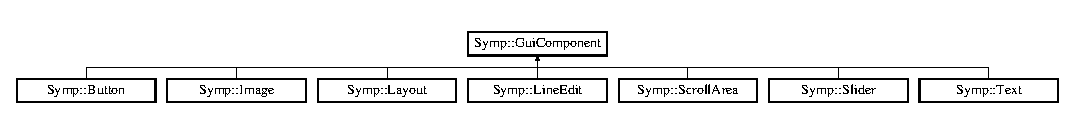
\includegraphics[height=1.151079cm]{class_symp_1_1_gui_component}
\end{center}
\end{figure}
\subsection*{Public Member Functions}
\begin{DoxyCompactItemize}
\item 
\hyperlink{class_symp_1_1_gui_component_a22124675c2976983ac18374f81cc3fb3}{Gui\-Component} ()
\begin{DoxyCompactList}\small\item\em \hyperlink{class_symp_1_1_gui_component}{Gui\-Component} constructor. Responsible for the initialization of the private attributes \hyperlink{class_symp_1_1_gui_component_ad4c3e34b824e1f9d6a030ca54fc1a7cf}{m\-\_\-i\-Width} and \hyperlink{class_symp_1_1_gui_component_aa84bb60b7aa1adb1522c63acff2909c2}{m\-\_\-i\-Height}, and for the creation of an I\-N\-D\-\_\-\-Entity2d. The static function \hyperlink{class_symp_1_1_gui_component_a05838e01bbf1e31f292ed4b92a520f20}{init()} is called only on the creation of the \hyperlink{class_symp_1_1_menu_manager}{Menu\-Manager} and allow the management of a I\-N\-D\-\_\-\-Entity2d by several Indielib managers. \end{DoxyCompactList}\item 
\hyperlink{class_symp_1_1_gui_component_ac05c461540b767c3670996a9f67ba0ba}{$\sim$\-Gui\-Component} ()
\begin{DoxyCompactList}\small\item\em \hyperlink{class_symp_1_1_gui_component}{Gui\-Component} destructor. The only attribute to destroy is the Entity2d. \end{DoxyCompactList}\item 
virtual void \hyperlink{class_symp_1_1_gui_component_add73e07ea0a3c9c1c90640e783a3b5de}{update} ()=0
\item 
bool \hyperlink{class_symp_1_1_gui_component_ab3c318bd857cbefa99c0d4848e8d5cc8}{is\-Targeted\-By\-Mouse} (int mouse\-X, int mouse\-Y)
\begin{DoxyCompactList}\small\item\em Check if the component is under the mouse This function is used in both clic event and mouse over event. Only a \hyperlink{class_symp_1_1_gui_component_a22124675c2976983ac18374f81cc3fb3}{Gui\-Component} is responsible for checking if the mouse is colliding its shape. \end{DoxyCompactList}\item 
bool \hyperlink{class_symp_1_1_gui_component_a1f8ff56c174ae9f4c32b31a0ed1a53b9}{load\-Font} ()
\begin{DoxyCompactList}\small\item\em Load a font file into the application. \end{DoxyCompactList}\item 
I\-N\-D\-\_\-\-Entity2d $\ast$ \hyperlink{class_symp_1_1_gui_component_a52ebebf0d3b3c7b6594de11d251fadf4}{get\-I\-N\-D\-\_\-\-Entity2d} () const 
\item 
float \hyperlink{class_symp_1_1_gui_component_a1abb4a355d333f5997d60d7b9f752181}{get\-Pos\-X} () const 
\item 
float \hyperlink{class_symp_1_1_gui_component_ac96015064a38de7a10f8b000fb59f7fe}{get\-Pos\-Y} () const 
\item 
bool \hyperlink{class_symp_1_1_gui_component_ab61bc0870020609f32e0035bbb171305}{is\-Hovered} () const 
\item 
bool \hyperlink{class_symp_1_1_gui_component_a26e2943ad705eac98fbac3bab4a8bb35}{is\-Enabled} () const 
\item 
int \hyperlink{class_symp_1_1_gui_component_a77b9f95708331850e2782b2d1b542ef2}{get\-Width} () const 
\item 
int \hyperlink{class_symp_1_1_gui_component_a4810b7562994b2371fa51a6d8a45203e}{get\-Height} () const 
\item 
void \hyperlink{class_symp_1_1_gui_component_ae3adbc8ba653a8f2d27df10e453df452}{enable} ()
\begin{DoxyCompactList}\small\item\em Enable a component When a \hyperlink{class_symp_1_1_gui_component_a22124675c2976983ac18374f81cc3fb3}{Gui\-Component} is enabled, it can receive any kind of event, and following its type, it can change its shape or color, in a ergonomic way. To make a \hyperlink{class_symp_1_1_gui_component_a22124675c2976983ac18374f81cc3fb3}{Gui\-Component} disabled, call the \hyperlink{class_symp_1_1_gui_component_a1666433de58fd568b568d1d48584802b}{disable()} function. \end{DoxyCompactList}\item 
void \hyperlink{class_symp_1_1_gui_component_a1666433de58fd568b568d1d48584802b}{disable} ()
\begin{DoxyCompactList}\small\item\em Disable a component When a \hyperlink{class_symp_1_1_gui_component_a22124675c2976983ac18374f81cc3fb3}{Gui\-Component} is disabled, it cant receive any kind of event, and following its type, it can change its shape or color, in a ergonomic way. To make a \hyperlink{class_symp_1_1_gui_component_a22124675c2976983ac18374f81cc3fb3}{Gui\-Component} enabled, call the \hyperlink{class_symp_1_1_gui_component_ae3adbc8ba653a8f2d27df10e453df452}{enable()} function. \end{DoxyCompactList}\item 
void \hyperlink{class_symp_1_1_gui_component_a34211085d9f971ef3a4e117b0603acf3}{show} ()
\begin{DoxyCompactList}\small\item\em Show the \hyperlink{class_symp_1_1_gui_component}{Gui\-Component}. \end{DoxyCompactList}\item 
void \hyperlink{class_symp_1_1_gui_component_a8fc95fe5807ba8b1afa599db48771c0d}{hide} ()
\begin{DoxyCompactList}\small\item\em Hide the \hyperlink{class_symp_1_1_gui_component}{Gui\-Component}. \end{DoxyCompactList}\item 
void \hyperlink{class_symp_1_1_gui_component_aac319b767afa5a945208c704d3d640ed}{set\-Hovered} (bool value)
\item 
void \hyperlink{class_symp_1_1_gui_component_ab6a2f0f5f43de649f1e50d601518bf1e}{set\-Surface} (const char $\ast$file\-Path)
\begin{DoxyCompactList}\small\item\em Apply a texture from an image file to a \hyperlink{class_symp_1_1_gui_component_a22124675c2976983ac18374f81cc3fb3}{Gui\-Component} For displaying a texture on an I\-N\-D\-\_\-\-Entity2d, Indielib library needs to have a I\-N\-D\-\_\-\-Surface object, and itself needs a I\-N\-D\-\_\-\-Image object. We initialize these objects by using static function of the Indielib managers initialized by \hyperlink{class_symp_1_1_gui_component_a05838e01bbf1e31f292ed4b92a520f20}{init()}. \end{DoxyCompactList}\item 
void \hyperlink{class_symp_1_1_gui_component_a35b54d009eeb7cf4790ca6f33f2d3906}{set\-Width} (int width)
\item 
void \hyperlink{class_symp_1_1_gui_component_a142f827392864e64b77ad02e05575f97}{set\-Height} (int height)
\item 
void \hyperlink{class_symp_1_1_gui_component_a56ec60b13aaf72bee8c3212d89986076}{set\-Rectangle} (int x, int y, int w, int h)
\item 
void \hyperlink{class_symp_1_1_gui_component_ae0939017b02f2aad37375ca2bb25f758}{set\-Position} (float p\-X, float p\-Y, int p\-Z)
\item 
void \hyperlink{class_symp_1_1_gui_component_a71b9ec5dbeb56658e12dc5d3872c5625}{set\-Scale} (float p\-Sx, float p\-Sy)
\item 
bool \hyperlink{class_symp_1_1_gui_component_acdbda4c1c82e319b7b0de755355216a0}{set\-Hot\-Spot} (float p\-X, float p\-Y)
\end{DoxyCompactItemize}
\subsection*{Static Public Member Functions}
\begin{DoxyCompactItemize}
\item 
static void \hyperlink{class_symp_1_1_gui_component_a05838e01bbf1e31f292ed4b92a520f20}{init} (\hyperlink{class_symp_1_1_render}{Render} $\ast$p\-Render)
\begin{DoxyCompactList}\small\item\em \hyperlink{class_symp_1_1_gui_component}{Gui\-Component} static initializer This static function is called by the \#\-Menu\-Manager at its creation. It started all the Indielib services that need I\-N\-D\-\_\-\-Entity2d to be managed and rendered. \end{DoxyCompactList}\item 
static void \hyperlink{class_symp_1_1_gui_component_a011075cc3a09e9a4494557fcb56dff18}{end} ()
\begin{DoxyCompactList}\small\item\em \hyperlink{class_symp_1_1_gui_component}{Gui\-Component} static destroyer This static function is called by the \#\-Menu\-Manager at its destruction. It kill all the Indielib services. \end{DoxyCompactList}\end{DoxyCompactItemize}
\subsection*{Protected Attributes}
\begin{DoxyCompactItemize}
\item 
I\-N\-D\-\_\-\-Font $\ast$ \hyperlink{class_symp_1_1_gui_component_a9704a149c8207503b3a7824b096b7b9f}{m\-\_\-p\-Font\-Small}
\item 
I\-N\-D\-\_\-\-Font $\ast$ \hyperlink{class_symp_1_1_gui_component_a784e1d58bb695ca95f12c1611f144488}{m\-\_\-p\-Font\-Big}
\item 
I\-N\-D\-\_\-\-Entity2d $\ast$ \hyperlink{class_symp_1_1_gui_component_ae2548627f8f866222e13347cc4284b24}{m\-\_\-p\-Entity2d}
\item 
int \hyperlink{class_symp_1_1_gui_component_ad4c3e34b824e1f9d6a030ca54fc1a7cf}{m\-\_\-i\-Width}
\item 
int \hyperlink{class_symp_1_1_gui_component_aa84bb60b7aa1adb1522c63acff2909c2}{m\-\_\-i\-Height}
\item 
bool \hyperlink{class_symp_1_1_gui_component_abb0e57a2b738621ed7e4aa89bf65e44e}{m\-\_\-b\-Is\-Hovered}
\item 
bool \hyperlink{class_symp_1_1_gui_component_af7a55b2a7e2f3e11c30a51f32571564f}{m\-\_\-b\-Is\-Enabled}
\end{DoxyCompactItemize}
\subsection*{Static Protected Attributes}
\begin{DoxyCompactItemize}
\item 
static I\-N\-D\-\_\-\-Image\-Manager $\ast$ \hyperlink{class_symp_1_1_gui_component_a7e1826a68cccf9b7a922e5f4176dba97}{s\-\_\-p\-Image\-Manager} = nullptr
\item 
static I\-N\-D\-\_\-\-Surface\-Manager $\ast$ \hyperlink{class_symp_1_1_gui_component_a768d28ae7ffce1d8a8025e6204f82ee5}{s\-\_\-p\-Surface\-Manager} = nullptr
\item 
static I\-N\-D\-\_\-\-Font\-Manager $\ast$ \hyperlink{class_symp_1_1_gui_component_a4c817ae1da9423d19b7d7455c29c614a}{s\-\_\-p\-Font\-Manager} = nullptr
\end{DoxyCompactItemize}


\subsection{Detailed Description}
\hyperlink{class_symp_1_1_gui_component}{Gui\-Component} facade for the creation of Menu graphical entities The \hyperlink{class_symp_1_1_gui_component}{Gui\-Component} class implements a facade of the Indielib I\-N\-D\-\_\-\-E\-Ntity2d elements for the unique use of the menus. Each graphical element that compose a menu inherits from the \hyperlink{class_symp_1_1_gui_component}{Gui\-Component} class. The elements are stored in the \#\-Menu\-Manager class and rendered/updated by the \#\-Game\-Manager class. In order to use the Indielib architecture, this class implements static method for the I\-N\-D\-\_\-\-Image\-Manager, I\-N\-D\-\_\-\-Surface\-Manager and the I\-N\-D\-\_\-\-Font\-Manager initialization destruction. 

\begin{DoxySeeAlso}{See Also}
\hyperlink{class_symp_1_1_menu_manager}{Menu\-Manager} 

\hyperlink{class_symp_1_1_game_manager_a53eae391ee3ea958e26d60b51516c770}{Game\-Manager\-::update\-Menu()} 

\hyperlink{class_symp_1_1_gui_component_a05838e01bbf1e31f292ed4b92a520f20}{Gui\-Component\-::init()} 

\hyperlink{class_symp_1_1_gui_component_a011075cc3a09e9a4494557fcb56dff18}{Gui\-Component\-::end()} 
\end{DoxySeeAlso}


Definition at line 67 of file Gui\-Component.\-h.



\subsection{Constructor \& Destructor Documentation}
\hypertarget{class_symp_1_1_gui_component_a22124675c2976983ac18374f81cc3fb3}{\index{Symp\-::\-Gui\-Component@{Symp\-::\-Gui\-Component}!Gui\-Component@{Gui\-Component}}
\index{Gui\-Component@{Gui\-Component}!Symp::GuiComponent@{Symp\-::\-Gui\-Component}}
\subsubsection[{Gui\-Component}]{\setlength{\rightskip}{0pt plus 5cm}Symp\-::\-Gui\-Component\-::\-Gui\-Component (
\begin{DoxyParamCaption}
{}
\end{DoxyParamCaption}
)}}\label{class_symp_1_1_gui_component_a22124675c2976983ac18374f81cc3fb3}


\hyperlink{class_symp_1_1_gui_component}{Gui\-Component} constructor. Responsible for the initialization of the private attributes \hyperlink{class_symp_1_1_gui_component_ad4c3e34b824e1f9d6a030ca54fc1a7cf}{m\-\_\-i\-Width} and \hyperlink{class_symp_1_1_gui_component_aa84bb60b7aa1adb1522c63acff2909c2}{m\-\_\-i\-Height}, and for the creation of an I\-N\-D\-\_\-\-Entity2d. The static function \hyperlink{class_symp_1_1_gui_component_a05838e01bbf1e31f292ed4b92a520f20}{init()} is called only on the creation of the \hyperlink{class_symp_1_1_menu_manager}{Menu\-Manager} and allow the management of a I\-N\-D\-\_\-\-Entity2d by several Indielib managers. 

\begin{DoxySeeAlso}{See Also}
\hyperlink{class_symp_1_1_gui_component_a05838e01bbf1e31f292ed4b92a520f20}{init()} 

\hyperlink{class_symp_1_1_gui_component_ac05c461540b767c3670996a9f67ba0ba}{$\sim$\-Gui\-Component()} 
\end{DoxySeeAlso}


Definition at line 31 of file Gui\-Component.\-cpp.

\hypertarget{class_symp_1_1_gui_component_ac05c461540b767c3670996a9f67ba0ba}{\index{Symp\-::\-Gui\-Component@{Symp\-::\-Gui\-Component}!$\sim$\-Gui\-Component@{$\sim$\-Gui\-Component}}
\index{$\sim$\-Gui\-Component@{$\sim$\-Gui\-Component}!Symp::GuiComponent@{Symp\-::\-Gui\-Component}}
\subsubsection[{$\sim$\-Gui\-Component}]{\setlength{\rightskip}{0pt plus 5cm}Symp\-::\-Gui\-Component\-::$\sim$\-Gui\-Component (
\begin{DoxyParamCaption}
{}
\end{DoxyParamCaption}
)}}\label{class_symp_1_1_gui_component_ac05c461540b767c3670996a9f67ba0ba}


\hyperlink{class_symp_1_1_gui_component}{Gui\-Component} destructor. The only attribute to destroy is the Entity2d. 

\begin{DoxySeeAlso}{See Also}
\hyperlink{class_symp_1_1_gui_component_a22124675c2976983ac18374f81cc3fb3}{Gui\-Component()} 
\end{DoxySeeAlso}


Definition at line 41 of file Gui\-Component.\-cpp.



\subsection{Member Function Documentation}
\hypertarget{class_symp_1_1_gui_component_a1666433de58fd568b568d1d48584802b}{\index{Symp\-::\-Gui\-Component@{Symp\-::\-Gui\-Component}!disable@{disable}}
\index{disable@{disable}!Symp::GuiComponent@{Symp\-::\-Gui\-Component}}
\subsubsection[{disable}]{\setlength{\rightskip}{0pt plus 5cm}void Symp\-::\-Gui\-Component\-::disable (
\begin{DoxyParamCaption}
{}
\end{DoxyParamCaption}
)}}\label{class_symp_1_1_gui_component_a1666433de58fd568b568d1d48584802b}


Disable a component When a \hyperlink{class_symp_1_1_gui_component_a22124675c2976983ac18374f81cc3fb3}{Gui\-Component} is disabled, it cant receive any kind of event, and following its type, it can change its shape or color, in a ergonomic way. To make a \hyperlink{class_symp_1_1_gui_component_a22124675c2976983ac18374f81cc3fb3}{Gui\-Component} enabled, call the \hyperlink{class_symp_1_1_gui_component_ae3adbc8ba653a8f2d27df10e453df452}{enable()} function. 

\begin{DoxySeeAlso}{See Also}
\hyperlink{class_symp_1_1_gui_component_af7a55b2a7e2f3e11c30a51f32571564f}{m\-\_\-b\-Is\-Enabled} 

\hyperlink{class_symp_1_1_gui_component_add73e07ea0a3c9c1c90640e783a3b5de}{update()} 

\hyperlink{class_symp_1_1_gui_component_ae3adbc8ba653a8f2d27df10e453df452}{enable()} 

\hyperlink{class_symp_1_1_gui_component_a22124675c2976983ac18374f81cc3fb3}{Gui\-Component()} 
\end{DoxySeeAlso}


Definition at line 106 of file Gui\-Component.\-cpp.

\hypertarget{class_symp_1_1_gui_component_ae3adbc8ba653a8f2d27df10e453df452}{\index{Symp\-::\-Gui\-Component@{Symp\-::\-Gui\-Component}!enable@{enable}}
\index{enable@{enable}!Symp::GuiComponent@{Symp\-::\-Gui\-Component}}
\subsubsection[{enable}]{\setlength{\rightskip}{0pt plus 5cm}void Symp\-::\-Gui\-Component\-::enable (
\begin{DoxyParamCaption}
{}
\end{DoxyParamCaption}
)}}\label{class_symp_1_1_gui_component_ae3adbc8ba653a8f2d27df10e453df452}


Enable a component When a \hyperlink{class_symp_1_1_gui_component_a22124675c2976983ac18374f81cc3fb3}{Gui\-Component} is enabled, it can receive any kind of event, and following its type, it can change its shape or color, in a ergonomic way. To make a \hyperlink{class_symp_1_1_gui_component_a22124675c2976983ac18374f81cc3fb3}{Gui\-Component} disabled, call the \hyperlink{class_symp_1_1_gui_component_a1666433de58fd568b568d1d48584802b}{disable()} function. 

\begin{DoxySeeAlso}{See Also}
\hyperlink{class_symp_1_1_gui_component_af7a55b2a7e2f3e11c30a51f32571564f}{m\-\_\-b\-Is\-Enabled} 

\hyperlink{class_symp_1_1_gui_component_add73e07ea0a3c9c1c90640e783a3b5de}{update()} 

\hyperlink{class_symp_1_1_gui_component_a1666433de58fd568b568d1d48584802b}{disable()} 

\hyperlink{class_symp_1_1_gui_component_a22124675c2976983ac18374f81cc3fb3}{Gui\-Component()} 
\end{DoxySeeAlso}


Definition at line 90 of file Gui\-Component.\-cpp.

\hypertarget{class_symp_1_1_gui_component_a011075cc3a09e9a4494557fcb56dff18}{\index{Symp\-::\-Gui\-Component@{Symp\-::\-Gui\-Component}!end@{end}}
\index{end@{end}!Symp::GuiComponent@{Symp\-::\-Gui\-Component}}
\subsubsection[{end}]{\setlength{\rightskip}{0pt plus 5cm}void Symp\-::\-Gui\-Component\-::end (
\begin{DoxyParamCaption}
{}
\end{DoxyParamCaption}
)\hspace{0.3cm}{\ttfamily [static]}}}\label{class_symp_1_1_gui_component_a011075cc3a09e9a4494557fcb56dff18}


\hyperlink{class_symp_1_1_gui_component}{Gui\-Component} static destroyer This static function is called by the \#\-Menu\-Manager at its destruction. It kill all the Indielib services. 

\begin{DoxySeeAlso}{See Also}
\hyperlink{class_symp_1_1_gui_component_a05838e01bbf1e31f292ed4b92a520f20}{init()} 

\hyperlink{class_symp_1_1_menu_manager}{Menu\-Manager} 

\hyperlink{class_symp_1_1_gui_component_a22124675c2976983ac18374f81cc3fb3}{Gui\-Component()} 

\hyperlink{class_symp_1_1_gui_component_ac05c461540b767c3670996a9f67ba0ba}{$\sim$\-Gui\-Component()} 
\end{DoxySeeAlso}


Definition at line 72 of file Gui\-Component.\-cpp.

\hypertarget{class_symp_1_1_gui_component_a4810b7562994b2371fa51a6d8a45203e}{\index{Symp\-::\-Gui\-Component@{Symp\-::\-Gui\-Component}!get\-Height@{get\-Height}}
\index{get\-Height@{get\-Height}!Symp::GuiComponent@{Symp\-::\-Gui\-Component}}
\subsubsection[{get\-Height}]{\setlength{\rightskip}{0pt plus 5cm}int Symp\-::\-Gui\-Component\-::get\-Height (
\begin{DoxyParamCaption}
{}
\end{DoxyParamCaption}
) const\hspace{0.3cm}{\ttfamily [inline]}}}\label{class_symp_1_1_gui_component_a4810b7562994b2371fa51a6d8a45203e}


Definition at line 86 of file Gui\-Component.\-h.

\hypertarget{class_symp_1_1_gui_component_a52ebebf0d3b3c7b6594de11d251fadf4}{\index{Symp\-::\-Gui\-Component@{Symp\-::\-Gui\-Component}!get\-I\-N\-D\-\_\-\-Entity2d@{get\-I\-N\-D\-\_\-\-Entity2d}}
\index{get\-I\-N\-D\-\_\-\-Entity2d@{get\-I\-N\-D\-\_\-\-Entity2d}!Symp::GuiComponent@{Symp\-::\-Gui\-Component}}
\subsubsection[{get\-I\-N\-D\-\_\-\-Entity2d}]{\setlength{\rightskip}{0pt plus 5cm}I\-N\-D\-\_\-\-Entity2d$\ast$ Symp\-::\-Gui\-Component\-::get\-I\-N\-D\-\_\-\-Entity2d (
\begin{DoxyParamCaption}
{}
\end{DoxyParamCaption}
) const\hspace{0.3cm}{\ttfamily [inline]}}}\label{class_symp_1_1_gui_component_a52ebebf0d3b3c7b6594de11d251fadf4}


Definition at line 80 of file Gui\-Component.\-h.

\hypertarget{class_symp_1_1_gui_component_a1abb4a355d333f5997d60d7b9f752181}{\index{Symp\-::\-Gui\-Component@{Symp\-::\-Gui\-Component}!get\-Pos\-X@{get\-Pos\-X}}
\index{get\-Pos\-X@{get\-Pos\-X}!Symp::GuiComponent@{Symp\-::\-Gui\-Component}}
\subsubsection[{get\-Pos\-X}]{\setlength{\rightskip}{0pt plus 5cm}float Symp\-::\-Gui\-Component\-::get\-Pos\-X (
\begin{DoxyParamCaption}
{}
\end{DoxyParamCaption}
) const\hspace{0.3cm}{\ttfamily [inline]}}}\label{class_symp_1_1_gui_component_a1abb4a355d333f5997d60d7b9f752181}


Definition at line 81 of file Gui\-Component.\-h.

\hypertarget{class_symp_1_1_gui_component_ac96015064a38de7a10f8b000fb59f7fe}{\index{Symp\-::\-Gui\-Component@{Symp\-::\-Gui\-Component}!get\-Pos\-Y@{get\-Pos\-Y}}
\index{get\-Pos\-Y@{get\-Pos\-Y}!Symp::GuiComponent@{Symp\-::\-Gui\-Component}}
\subsubsection[{get\-Pos\-Y}]{\setlength{\rightskip}{0pt plus 5cm}float Symp\-::\-Gui\-Component\-::get\-Pos\-Y (
\begin{DoxyParamCaption}
{}
\end{DoxyParamCaption}
) const\hspace{0.3cm}{\ttfamily [inline]}}}\label{class_symp_1_1_gui_component_ac96015064a38de7a10f8b000fb59f7fe}


Definition at line 82 of file Gui\-Component.\-h.

\hypertarget{class_symp_1_1_gui_component_a77b9f95708331850e2782b2d1b542ef2}{\index{Symp\-::\-Gui\-Component@{Symp\-::\-Gui\-Component}!get\-Width@{get\-Width}}
\index{get\-Width@{get\-Width}!Symp::GuiComponent@{Symp\-::\-Gui\-Component}}
\subsubsection[{get\-Width}]{\setlength{\rightskip}{0pt plus 5cm}int Symp\-::\-Gui\-Component\-::get\-Width (
\begin{DoxyParamCaption}
{}
\end{DoxyParamCaption}
) const\hspace{0.3cm}{\ttfamily [inline]}}}\label{class_symp_1_1_gui_component_a77b9f95708331850e2782b2d1b542ef2}


Definition at line 85 of file Gui\-Component.\-h.

\hypertarget{class_symp_1_1_gui_component_a8fc95fe5807ba8b1afa599db48771c0d}{\index{Symp\-::\-Gui\-Component@{Symp\-::\-Gui\-Component}!hide@{hide}}
\index{hide@{hide}!Symp::GuiComponent@{Symp\-::\-Gui\-Component}}
\subsubsection[{hide}]{\setlength{\rightskip}{0pt plus 5cm}void Symp\-::\-Gui\-Component\-::hide (
\begin{DoxyParamCaption}
{}
\end{DoxyParamCaption}
)}}\label{class_symp_1_1_gui_component_a8fc95fe5807ba8b1afa599db48771c0d}


Hide the \hyperlink{class_symp_1_1_gui_component}{Gui\-Component}. 

\begin{DoxySeeAlso}{See Also}
\hyperlink{class_symp_1_1_gui_component_a34211085d9f971ef3a4e117b0603acf3}{show()} 

\hyperlink{class_symp_1_1_gui_component}{Gui\-Component} 
\end{DoxySeeAlso}


Definition at line 127 of file Gui\-Component.\-cpp.

\hypertarget{class_symp_1_1_gui_component_a05838e01bbf1e31f292ed4b92a520f20}{\index{Symp\-::\-Gui\-Component@{Symp\-::\-Gui\-Component}!init@{init}}
\index{init@{init}!Symp::GuiComponent@{Symp\-::\-Gui\-Component}}
\subsubsection[{init}]{\setlength{\rightskip}{0pt plus 5cm}void Symp\-::\-Gui\-Component\-::init (
\begin{DoxyParamCaption}
\item[{{\bf Render} $\ast$}]{p\-Render}
\end{DoxyParamCaption}
)\hspace{0.3cm}{\ttfamily [static]}}}\label{class_symp_1_1_gui_component_a05838e01bbf1e31f292ed4b92a520f20}


\hyperlink{class_symp_1_1_gui_component}{Gui\-Component} static initializer This static function is called by the \#\-Menu\-Manager at its creation. It started all the Indielib services that need I\-N\-D\-\_\-\-Entity2d to be managed and rendered. 


\begin{DoxyParams}{Parameters}
{\em p\-Render} & the reference to the \#\-Render class \\
\hline
\end{DoxyParams}
\begin{DoxySeeAlso}{See Also}
\hyperlink{class_symp_1_1_menu_manager}{Menu\-Manager} 

\hyperlink{class_symp_1_1_gui_component_a011075cc3a09e9a4494557fcb56dff18}{end()} 

\hyperlink{class_symp_1_1_gui_component_a22124675c2976983ac18374f81cc3fb3}{Gui\-Component()} 

\hyperlink{class_symp_1_1_gui_component_ac05c461540b767c3670996a9f67ba0ba}{$\sim$\-Gui\-Component()} 
\end{DoxySeeAlso}


Definition at line 55 of file Gui\-Component.\-cpp.

\hypertarget{class_symp_1_1_gui_component_a26e2943ad705eac98fbac3bab4a8bb35}{\index{Symp\-::\-Gui\-Component@{Symp\-::\-Gui\-Component}!is\-Enabled@{is\-Enabled}}
\index{is\-Enabled@{is\-Enabled}!Symp::GuiComponent@{Symp\-::\-Gui\-Component}}
\subsubsection[{is\-Enabled}]{\setlength{\rightskip}{0pt plus 5cm}bool Symp\-::\-Gui\-Component\-::is\-Enabled (
\begin{DoxyParamCaption}
{}
\end{DoxyParamCaption}
) const\hspace{0.3cm}{\ttfamily [inline]}}}\label{class_symp_1_1_gui_component_a26e2943ad705eac98fbac3bab4a8bb35}


Definition at line 84 of file Gui\-Component.\-h.

\hypertarget{class_symp_1_1_gui_component_ab61bc0870020609f32e0035bbb171305}{\index{Symp\-::\-Gui\-Component@{Symp\-::\-Gui\-Component}!is\-Hovered@{is\-Hovered}}
\index{is\-Hovered@{is\-Hovered}!Symp::GuiComponent@{Symp\-::\-Gui\-Component}}
\subsubsection[{is\-Hovered}]{\setlength{\rightskip}{0pt plus 5cm}bool Symp\-::\-Gui\-Component\-::is\-Hovered (
\begin{DoxyParamCaption}
{}
\end{DoxyParamCaption}
) const\hspace{0.3cm}{\ttfamily [inline]}}}\label{class_symp_1_1_gui_component_ab61bc0870020609f32e0035bbb171305}


Definition at line 83 of file Gui\-Component.\-h.

\hypertarget{class_symp_1_1_gui_component_ab3c318bd857cbefa99c0d4848e8d5cc8}{\index{Symp\-::\-Gui\-Component@{Symp\-::\-Gui\-Component}!is\-Targeted\-By\-Mouse@{is\-Targeted\-By\-Mouse}}
\index{is\-Targeted\-By\-Mouse@{is\-Targeted\-By\-Mouse}!Symp::GuiComponent@{Symp\-::\-Gui\-Component}}
\subsubsection[{is\-Targeted\-By\-Mouse}]{\setlength{\rightskip}{0pt plus 5cm}bool Symp\-::\-Gui\-Component\-::is\-Targeted\-By\-Mouse (
\begin{DoxyParamCaption}
\item[{int}]{mouse\-X, }
\item[{int}]{mouse\-Y}
\end{DoxyParamCaption}
)}}\label{class_symp_1_1_gui_component_ab3c318bd857cbefa99c0d4848e8d5cc8}


Check if the component is under the mouse This function is used in both clic event and mouse over event. Only a \hyperlink{class_symp_1_1_gui_component_a22124675c2976983ac18374f81cc3fb3}{Gui\-Component} is responsible for checking if the mouse is colliding its shape. 


\begin{DoxyParams}{Parameters}
{\em mouse\-X} & the x coordinate of the mouse position in pixels \\
\hline
{\em mouse\-Y} & the y coordinate of the mouse position in pixels \\
\hline
\end{DoxyParams}
\begin{DoxySeeAlso}{See Also}
\hyperlink{class_symp_1_1_gui_component_a22124675c2976983ac18374f81cc3fb3}{Gui\-Component()} 

\hyperlink{class_symp_1_1_menu_manager_ad72c273480039d17ebda3480311d4508}{Menu\-Manager\-::handle\-Mouse\-Clic()} 

\hyperlink{class_symp_1_1_menu_manager_adfcb55f36a13d91538c789fdc4f5dd14}{Menu\-Manager\-::handle\-Mouse\-Hover()} 
\end{DoxySeeAlso}


Definition at line 155 of file Gui\-Component.\-cpp.

\hypertarget{class_symp_1_1_gui_component_a1f8ff56c174ae9f4c32b31a0ed1a53b9}{\index{Symp\-::\-Gui\-Component@{Symp\-::\-Gui\-Component}!load\-Font@{load\-Font}}
\index{load\-Font@{load\-Font}!Symp::GuiComponent@{Symp\-::\-Gui\-Component}}
\subsubsection[{load\-Font}]{\setlength{\rightskip}{0pt plus 5cm}bool Symp\-::\-Gui\-Component\-::load\-Font (
\begin{DoxyParamCaption}
{}
\end{DoxyParamCaption}
)}}\label{class_symp_1_1_gui_component_a1f8ff56c174ae9f4c32b31a0ed1a53b9}


Load a font file into the application. 

\begin{DoxyRefDesc}{Bug}
\item[\hyperlink{bug__bug000002}{Bug}]/!\textbackslash{} N\-O\-T R\-E\-A\-D\-Y Y\-E\-T /!\textbackslash{} This function need the newest version of Indielib to load Angel\-Code font. \end{DoxyRefDesc}

\begin{DoxyParams}{Parameters}
{\em file\-Path} & the path to the font file \\
\hline
\end{DoxyParams}
\begin{DoxySeeAlso}{See Also}
\hyperlink{class_symp_1_1_gui_component_a22124675c2976983ac18374f81cc3fb3}{Gui\-Component()} 
\end{DoxySeeAlso}


Definition at line 137 of file Gui\-Component.\-cpp.

\hypertarget{class_symp_1_1_gui_component_a142f827392864e64b77ad02e05575f97}{\index{Symp\-::\-Gui\-Component@{Symp\-::\-Gui\-Component}!set\-Height@{set\-Height}}
\index{set\-Height@{set\-Height}!Symp::GuiComponent@{Symp\-::\-Gui\-Component}}
\subsubsection[{set\-Height}]{\setlength{\rightskip}{0pt plus 5cm}void Symp\-::\-Gui\-Component\-::set\-Height (
\begin{DoxyParamCaption}
\item[{int}]{height}
\end{DoxyParamCaption}
)\hspace{0.3cm}{\ttfamily [inline]}}}\label{class_symp_1_1_gui_component_a142f827392864e64b77ad02e05575f97}


Definition at line 96 of file Gui\-Component.\-h.

\hypertarget{class_symp_1_1_gui_component_acdbda4c1c82e319b7b0de755355216a0}{\index{Symp\-::\-Gui\-Component@{Symp\-::\-Gui\-Component}!set\-Hot\-Spot@{set\-Hot\-Spot}}
\index{set\-Hot\-Spot@{set\-Hot\-Spot}!Symp::GuiComponent@{Symp\-::\-Gui\-Component}}
\subsubsection[{set\-Hot\-Spot}]{\setlength{\rightskip}{0pt plus 5cm}bool Symp\-::\-Gui\-Component\-::set\-Hot\-Spot (
\begin{DoxyParamCaption}
\item[{float}]{p\-X, }
\item[{float}]{p\-Y}
\end{DoxyParamCaption}
)\hspace{0.3cm}{\ttfamily [inline]}}}\label{class_symp_1_1_gui_component_acdbda4c1c82e319b7b0de755355216a0}


Definition at line 100 of file Gui\-Component.\-h.

\hypertarget{class_symp_1_1_gui_component_aac319b767afa5a945208c704d3d640ed}{\index{Symp\-::\-Gui\-Component@{Symp\-::\-Gui\-Component}!set\-Hovered@{set\-Hovered}}
\index{set\-Hovered@{set\-Hovered}!Symp::GuiComponent@{Symp\-::\-Gui\-Component}}
\subsubsection[{set\-Hovered}]{\setlength{\rightskip}{0pt plus 5cm}void Symp\-::\-Gui\-Component\-::set\-Hovered (
\begin{DoxyParamCaption}
\item[{bool}]{value}
\end{DoxyParamCaption}
)\hspace{0.3cm}{\ttfamily [inline]}}}\label{class_symp_1_1_gui_component_aac319b767afa5a945208c704d3d640ed}


Definition at line 93 of file Gui\-Component.\-h.

\hypertarget{class_symp_1_1_gui_component_ae0939017b02f2aad37375ca2bb25f758}{\index{Symp\-::\-Gui\-Component@{Symp\-::\-Gui\-Component}!set\-Position@{set\-Position}}
\index{set\-Position@{set\-Position}!Symp::GuiComponent@{Symp\-::\-Gui\-Component}}
\subsubsection[{set\-Position}]{\setlength{\rightskip}{0pt plus 5cm}void Symp\-::\-Gui\-Component\-::set\-Position (
\begin{DoxyParamCaption}
\item[{float}]{p\-X, }
\item[{float}]{p\-Y, }
\item[{int}]{p\-Z}
\end{DoxyParamCaption}
)\hspace{0.3cm}{\ttfamily [inline]}}}\label{class_symp_1_1_gui_component_ae0939017b02f2aad37375ca2bb25f758}


Definition at line 98 of file Gui\-Component.\-h.

\hypertarget{class_symp_1_1_gui_component_a56ec60b13aaf72bee8c3212d89986076}{\index{Symp\-::\-Gui\-Component@{Symp\-::\-Gui\-Component}!set\-Rectangle@{set\-Rectangle}}
\index{set\-Rectangle@{set\-Rectangle}!Symp::GuiComponent@{Symp\-::\-Gui\-Component}}
\subsubsection[{set\-Rectangle}]{\setlength{\rightskip}{0pt plus 5cm}void Symp\-::\-Gui\-Component\-::set\-Rectangle (
\begin{DoxyParamCaption}
\item[{int}]{x, }
\item[{int}]{y, }
\item[{int}]{w, }
\item[{int}]{h}
\end{DoxyParamCaption}
)}}\label{class_symp_1_1_gui_component_a56ec60b13aaf72bee8c3212d89986076}
\hypertarget{class_symp_1_1_gui_component_a71b9ec5dbeb56658e12dc5d3872c5625}{\index{Symp\-::\-Gui\-Component@{Symp\-::\-Gui\-Component}!set\-Scale@{set\-Scale}}
\index{set\-Scale@{set\-Scale}!Symp::GuiComponent@{Symp\-::\-Gui\-Component}}
\subsubsection[{set\-Scale}]{\setlength{\rightskip}{0pt plus 5cm}void Symp\-::\-Gui\-Component\-::set\-Scale (
\begin{DoxyParamCaption}
\item[{float}]{p\-Sx, }
\item[{float}]{p\-Sy}
\end{DoxyParamCaption}
)\hspace{0.3cm}{\ttfamily [inline]}}}\label{class_symp_1_1_gui_component_a71b9ec5dbeb56658e12dc5d3872c5625}


Definition at line 99 of file Gui\-Component.\-h.

\hypertarget{class_symp_1_1_gui_component_ab6a2f0f5f43de649f1e50d601518bf1e}{\index{Symp\-::\-Gui\-Component@{Symp\-::\-Gui\-Component}!set\-Surface@{set\-Surface}}
\index{set\-Surface@{set\-Surface}!Symp::GuiComponent@{Symp\-::\-Gui\-Component}}
\subsubsection[{set\-Surface}]{\setlength{\rightskip}{0pt plus 5cm}void Symp\-::\-Gui\-Component\-::set\-Surface (
\begin{DoxyParamCaption}
\item[{const char $\ast$}]{file\-Path}
\end{DoxyParamCaption}
)}}\label{class_symp_1_1_gui_component_ab6a2f0f5f43de649f1e50d601518bf1e}


Apply a texture from an image file to a \hyperlink{class_symp_1_1_gui_component_a22124675c2976983ac18374f81cc3fb3}{Gui\-Component} For displaying a texture on an I\-N\-D\-\_\-\-Entity2d, Indielib library needs to have a I\-N\-D\-\_\-\-Surface object, and itself needs a I\-N\-D\-\_\-\-Image object. We initialize these objects by using static function of the Indielib managers initialized by \hyperlink{class_symp_1_1_gui_component_a05838e01bbf1e31f292ed4b92a520f20}{init()}. 


\begin{DoxyParams}{Parameters}
{\em file\-Path} & the path to the image file \\
\hline
\end{DoxyParams}
\begin{DoxySeeAlso}{See Also}
\hyperlink{class_symp_1_1_gui_component_a22124675c2976983ac18374f81cc3fb3}{Gui\-Component()} 

\hyperlink{class_symp_1_1_gui_component_a05838e01bbf1e31f292ed4b92a520f20}{init()} 

\hyperlink{class_symp_1_1_gui_component_a011075cc3a09e9a4494557fcb56dff18}{end()} 
\end{DoxySeeAlso}


Definition at line 175 of file Gui\-Component.\-cpp.

\hypertarget{class_symp_1_1_gui_component_a35b54d009eeb7cf4790ca6f33f2d3906}{\index{Symp\-::\-Gui\-Component@{Symp\-::\-Gui\-Component}!set\-Width@{set\-Width}}
\index{set\-Width@{set\-Width}!Symp::GuiComponent@{Symp\-::\-Gui\-Component}}
\subsubsection[{set\-Width}]{\setlength{\rightskip}{0pt plus 5cm}void Symp\-::\-Gui\-Component\-::set\-Width (
\begin{DoxyParamCaption}
\item[{int}]{width}
\end{DoxyParamCaption}
)\hspace{0.3cm}{\ttfamily [inline]}}}\label{class_symp_1_1_gui_component_a35b54d009eeb7cf4790ca6f33f2d3906}


Definition at line 95 of file Gui\-Component.\-h.

\hypertarget{class_symp_1_1_gui_component_a34211085d9f971ef3a4e117b0603acf3}{\index{Symp\-::\-Gui\-Component@{Symp\-::\-Gui\-Component}!show@{show}}
\index{show@{show}!Symp::GuiComponent@{Symp\-::\-Gui\-Component}}
\subsubsection[{show}]{\setlength{\rightskip}{0pt plus 5cm}void Symp\-::\-Gui\-Component\-::show (
\begin{DoxyParamCaption}
{}
\end{DoxyParamCaption}
)}}\label{class_symp_1_1_gui_component_a34211085d9f971ef3a4e117b0603acf3}


Show the \hyperlink{class_symp_1_1_gui_component}{Gui\-Component}. 

\begin{DoxySeeAlso}{See Also}
\hyperlink{class_symp_1_1_gui_component_a8fc95fe5807ba8b1afa599db48771c0d}{hide()} 

\hyperlink{class_symp_1_1_gui_component}{Gui\-Component} 
\end{DoxySeeAlso}


Definition at line 118 of file Gui\-Component.\-cpp.

\hypertarget{class_symp_1_1_gui_component_add73e07ea0a3c9c1c90640e783a3b5de}{\index{Symp\-::\-Gui\-Component@{Symp\-::\-Gui\-Component}!update@{update}}
\index{update@{update}!Symp::GuiComponent@{Symp\-::\-Gui\-Component}}
\subsubsection[{update}]{\setlength{\rightskip}{0pt plus 5cm}virtual void Symp\-::\-Gui\-Component\-::update (
\begin{DoxyParamCaption}
{}
\end{DoxyParamCaption}
)\hspace{0.3cm}{\ttfamily [pure virtual]}}}\label{class_symp_1_1_gui_component_add73e07ea0a3c9c1c90640e783a3b5de}


Implemented in \hyperlink{class_symp_1_1_layout_a34a3df4f1637d1a95015e19a1ecf7fb4}{Symp\-::\-Layout}, \hyperlink{class_symp_1_1_image_a8de69cca37efc613094cfd1311ea1e13}{Symp\-::\-Image}, \hyperlink{class_symp_1_1_button_a5cec3a7ede8af0c059d6430f971b276b}{Symp\-::\-Button}, \hyperlink{class_symp_1_1_scroll_area_a9183e9193ecfa8a2d9fda6ff4d706680}{Symp\-::\-Scroll\-Area}, \hyperlink{class_symp_1_1_slider_ab010de4ff23eef8a6cc6706e9902209f}{Symp\-::\-Slider}, \hyperlink{class_symp_1_1_line_edit_a7742de762d2f74e87050ee4086aec9ae}{Symp\-::\-Line\-Edit}, and \hyperlink{class_symp_1_1_text_ab11eff488943981a0009549b77249a46}{Symp\-::\-Text}.



\subsection{Member Data Documentation}
\hypertarget{class_symp_1_1_gui_component_af7a55b2a7e2f3e11c30a51f32571564f}{\index{Symp\-::\-Gui\-Component@{Symp\-::\-Gui\-Component}!m\-\_\-b\-Is\-Enabled@{m\-\_\-b\-Is\-Enabled}}
\index{m\-\_\-b\-Is\-Enabled@{m\-\_\-b\-Is\-Enabled}!Symp::GuiComponent@{Symp\-::\-Gui\-Component}}
\subsubsection[{m\-\_\-b\-Is\-Enabled}]{\setlength{\rightskip}{0pt plus 5cm}bool Symp\-::\-Gui\-Component\-::m\-\_\-b\-Is\-Enabled\hspace{0.3cm}{\ttfamily [protected]}}}\label{class_symp_1_1_gui_component_af7a55b2a7e2f3e11c30a51f32571564f}
boolean that allow or not the events 

Definition at line 112 of file Gui\-Component.\-h.

\hypertarget{class_symp_1_1_gui_component_abb0e57a2b738621ed7e4aa89bf65e44e}{\index{Symp\-::\-Gui\-Component@{Symp\-::\-Gui\-Component}!m\-\_\-b\-Is\-Hovered@{m\-\_\-b\-Is\-Hovered}}
\index{m\-\_\-b\-Is\-Hovered@{m\-\_\-b\-Is\-Hovered}!Symp::GuiComponent@{Symp\-::\-Gui\-Component}}
\subsubsection[{m\-\_\-b\-Is\-Hovered}]{\setlength{\rightskip}{0pt plus 5cm}bool Symp\-::\-Gui\-Component\-::m\-\_\-b\-Is\-Hovered\hspace{0.3cm}{\ttfamily [protected]}}}\label{class_symp_1_1_gui_component_abb0e57a2b738621ed7e4aa89bf65e44e}
boolean that is updated with events 

Definition at line 111 of file Gui\-Component.\-h.

\hypertarget{class_symp_1_1_gui_component_aa84bb60b7aa1adb1522c63acff2909c2}{\index{Symp\-::\-Gui\-Component@{Symp\-::\-Gui\-Component}!m\-\_\-i\-Height@{m\-\_\-i\-Height}}
\index{m\-\_\-i\-Height@{m\-\_\-i\-Height}!Symp::GuiComponent@{Symp\-::\-Gui\-Component}}
\subsubsection[{m\-\_\-i\-Height}]{\setlength{\rightskip}{0pt plus 5cm}int Symp\-::\-Gui\-Component\-::m\-\_\-i\-Height\hspace{0.3cm}{\ttfamily [protected]}}}\label{class_symp_1_1_gui_component_aa84bb60b7aa1adb1522c63acff2909c2}
the height of the component in pixels 

Definition at line 110 of file Gui\-Component.\-h.

\hypertarget{class_symp_1_1_gui_component_ad4c3e34b824e1f9d6a030ca54fc1a7cf}{\index{Symp\-::\-Gui\-Component@{Symp\-::\-Gui\-Component}!m\-\_\-i\-Width@{m\-\_\-i\-Width}}
\index{m\-\_\-i\-Width@{m\-\_\-i\-Width}!Symp::GuiComponent@{Symp\-::\-Gui\-Component}}
\subsubsection[{m\-\_\-i\-Width}]{\setlength{\rightskip}{0pt plus 5cm}int Symp\-::\-Gui\-Component\-::m\-\_\-i\-Width\hspace{0.3cm}{\ttfamily [protected]}}}\label{class_symp_1_1_gui_component_ad4c3e34b824e1f9d6a030ca54fc1a7cf}
the width of the component in pixels 

Definition at line 109 of file Gui\-Component.\-h.

\hypertarget{class_symp_1_1_gui_component_ae2548627f8f866222e13347cc4284b24}{\index{Symp\-::\-Gui\-Component@{Symp\-::\-Gui\-Component}!m\-\_\-p\-Entity2d@{m\-\_\-p\-Entity2d}}
\index{m\-\_\-p\-Entity2d@{m\-\_\-p\-Entity2d}!Symp::GuiComponent@{Symp\-::\-Gui\-Component}}
\subsubsection[{m\-\_\-p\-Entity2d}]{\setlength{\rightskip}{0pt plus 5cm}I\-N\-D\-\_\-\-Entity2d$\ast$ Symp\-::\-Gui\-Component\-::m\-\_\-p\-Entity2d\hspace{0.3cm}{\ttfamily [protected]}}}\label{class_symp_1_1_gui_component_ae2548627f8f866222e13347cc4284b24}
the reference to the Indielib I\-N\-D\-\_\-\-Entity2d that stores the entities 

Definition at line 105 of file Gui\-Component.\-h.

\hypertarget{class_symp_1_1_gui_component_a784e1d58bb695ca95f12c1611f144488}{\index{Symp\-::\-Gui\-Component@{Symp\-::\-Gui\-Component}!m\-\_\-p\-Font\-Big@{m\-\_\-p\-Font\-Big}}
\index{m\-\_\-p\-Font\-Big@{m\-\_\-p\-Font\-Big}!Symp::GuiComponent@{Symp\-::\-Gui\-Component}}
\subsubsection[{m\-\_\-p\-Font\-Big}]{\setlength{\rightskip}{0pt plus 5cm}I\-N\-D\-\_\-\-Font$\ast$ Symp\-::\-Gui\-Component\-::m\-\_\-p\-Font\-Big\hspace{0.3cm}{\ttfamily [protected]}}}\label{class_symp_1_1_gui_component_a784e1d58bb695ca95f12c1611f144488}


Definition at line 104 of file Gui\-Component.\-h.

\hypertarget{class_symp_1_1_gui_component_a9704a149c8207503b3a7824b096b7b9f}{\index{Symp\-::\-Gui\-Component@{Symp\-::\-Gui\-Component}!m\-\_\-p\-Font\-Small@{m\-\_\-p\-Font\-Small}}
\index{m\-\_\-p\-Font\-Small@{m\-\_\-p\-Font\-Small}!Symp::GuiComponent@{Symp\-::\-Gui\-Component}}
\subsubsection[{m\-\_\-p\-Font\-Small}]{\setlength{\rightskip}{0pt plus 5cm}I\-N\-D\-\_\-\-Font$\ast$ Symp\-::\-Gui\-Component\-::m\-\_\-p\-Font\-Small\hspace{0.3cm}{\ttfamily [protected]}}}\label{class_symp_1_1_gui_component_a9704a149c8207503b3a7824b096b7b9f}


Definition at line 103 of file Gui\-Component.\-h.

\hypertarget{class_symp_1_1_gui_component_a4c817ae1da9423d19b7d7455c29c614a}{\index{Symp\-::\-Gui\-Component@{Symp\-::\-Gui\-Component}!s\-\_\-p\-Font\-Manager@{s\-\_\-p\-Font\-Manager}}
\index{s\-\_\-p\-Font\-Manager@{s\-\_\-p\-Font\-Manager}!Symp::GuiComponent@{Symp\-::\-Gui\-Component}}
\subsubsection[{s\-\_\-p\-Font\-Manager}]{\setlength{\rightskip}{0pt plus 5cm}I\-N\-D\-\_\-\-Font\-Manager $\ast$ Symp\-::\-Gui\-Component\-::s\-\_\-p\-Font\-Manager = nullptr\hspace{0.3cm}{\ttfamily [static]}, {\ttfamily [protected]}}}\label{class_symp_1_1_gui_component_a4c817ae1da9423d19b7d7455c29c614a}
static variable that references the Indielib I\-N\-D\-\_\-\-T\-T\-F\-\_\-\-Font\-Manager 

Definition at line 108 of file Gui\-Component.\-h.

\hypertarget{class_symp_1_1_gui_component_a7e1826a68cccf9b7a922e5f4176dba97}{\index{Symp\-::\-Gui\-Component@{Symp\-::\-Gui\-Component}!s\-\_\-p\-Image\-Manager@{s\-\_\-p\-Image\-Manager}}
\index{s\-\_\-p\-Image\-Manager@{s\-\_\-p\-Image\-Manager}!Symp::GuiComponent@{Symp\-::\-Gui\-Component}}
\subsubsection[{s\-\_\-p\-Image\-Manager}]{\setlength{\rightskip}{0pt plus 5cm}I\-N\-D\-\_\-\-Image\-Manager $\ast$ Symp\-::\-Gui\-Component\-::s\-\_\-p\-Image\-Manager = nullptr\hspace{0.3cm}{\ttfamily [static]}, {\ttfamily [protected]}}}\label{class_symp_1_1_gui_component_a7e1826a68cccf9b7a922e5f4176dba97}
static variable that references the Indielib I\-N\-D\-\_\-\-Image\-Manager 

Definition at line 106 of file Gui\-Component.\-h.

\hypertarget{class_symp_1_1_gui_component_a768d28ae7ffce1d8a8025e6204f82ee5}{\index{Symp\-::\-Gui\-Component@{Symp\-::\-Gui\-Component}!s\-\_\-p\-Surface\-Manager@{s\-\_\-p\-Surface\-Manager}}
\index{s\-\_\-p\-Surface\-Manager@{s\-\_\-p\-Surface\-Manager}!Symp::GuiComponent@{Symp\-::\-Gui\-Component}}
\subsubsection[{s\-\_\-p\-Surface\-Manager}]{\setlength{\rightskip}{0pt plus 5cm}I\-N\-D\-\_\-\-Surface\-Manager $\ast$ Symp\-::\-Gui\-Component\-::s\-\_\-p\-Surface\-Manager = nullptr\hspace{0.3cm}{\ttfamily [static]}, {\ttfamily [protected]}}}\label{class_symp_1_1_gui_component_a768d28ae7ffce1d8a8025e6204f82ee5}
static variable that references the Indielib I\-N\-D\-\_\-\-Surface\-Manager 

Definition at line 107 of file Gui\-Component.\-h.



The documentation for this class was generated from the following files\-:\begin{DoxyCompactItemize}
\item 
/home/cecilia/\-Documents/\-Symptogen/src/menu/\hyperlink{_gui_component_8h}{Gui\-Component.\-h}\item 
/home/cecilia/\-Documents/\-Symptogen/src/menu/\hyperlink{_gui_component_8cpp}{Gui\-Component.\-cpp}\end{DoxyCompactItemize}

\hypertarget{class_symp_1_1_headache}{\section{Symp\-:\-:Headache Class Reference}
\label{class_symp_1_1_headache}\index{Symp\-::\-Headache@{Symp\-::\-Headache}}
}


{\ttfamily \#include $<$Headache.\-h$>$}

Inheritance diagram for Symp\-:\-:Headache\-:\begin{figure}[H]
\begin{center}
\leavevmode
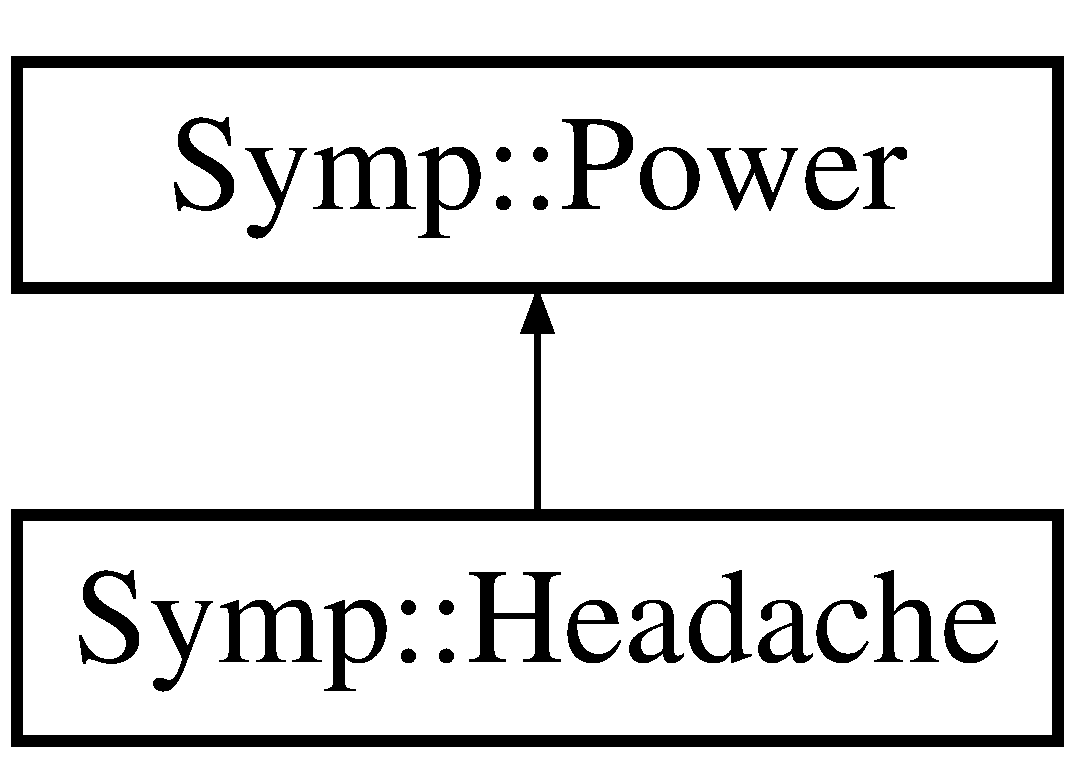
\includegraphics[height=2.000000cm]{class_symp_1_1_headache}
\end{center}
\end{figure}
\subsection*{Public Member Functions}
\begin{DoxyCompactItemize}
\item 
\hyperlink{class_symp_1_1_headache_a26cf6da6951ee941717d37d85c588a88}{Headache} ()
\begin{DoxyCompactList}\small\item\em \hyperlink{class_symp_1_1_headache}{Headache} class constructor. \end{DoxyCompactList}\item 
\hyperlink{class_symp_1_1_headache_ac739f61635fa88fdf1a337d855adb793}{$\sim$\-Headache} ()
\begin{DoxyCompactList}\small\item\em \hyperlink{class_symp_1_1_headache}{Headache} class destructor. \end{DoxyCompactList}\item 
void \hyperlink{class_symp_1_1_headache_a5de12b8de4529142a63e738132292e83}{execute} ()
\begin{DoxyCompactList}\small\item\em Implementation of the \hyperlink{class_symp_1_1_power}{Power} abstract class If the \hyperlink{class_symp_1_1_headache}{Headache} power is activated, this method will be called at each turn of the main loop. This method will make the character's temperature change, or not. \end{DoxyCompactList}\item 
void \hyperlink{class_symp_1_1_headache_adfb5b616e538d1c62062b854cdae464d}{force\-Execution} ()
\begin{DoxyCompactList}\small\item\em Force the execution of the \hyperlink{class_symp_1_1_headache}{Headache}. This test function is used by the developers to easely trigger the power of hot \hyperlink{class_symp_1_1_headache}{Headache} (temperature $>$ 0) or cold fever (temperature $<$ 0). \end{DoxyCompactList}\item 
unsigned int \hyperlink{class_symp_1_1_headache_aa65ea728ce75f6f3bdff9399d2235c4f}{get\-Last\-Execution} () const 
\item 
int \hyperlink{class_symp_1_1_headache_adcb2f0e2cb987f1678efae7f97100533}{get\-Rotation\-Angle} () const 
\item 
int \hyperlink{class_symp_1_1_headache_afb523ed96f5d079260573061da25dfa8}{get\-Max\-Rotation\-Agnle} () const 
\item 
int \hyperlink{class_symp_1_1_headache_a311375899d8e1266294566f02d6c0214}{get\-Interpolate\-Angle} () const 
\item 
unsigned int \hyperlink{class_symp_1_1_headache_ac158048ed0cb57c945a1a2ccee831b7c}{get\-Time\-To\-Trigger\-Random\-Headache} () const 
\item 
void \hyperlink{class_symp_1_1_headache_af6f3c9d87fe7b3f268943c90b382fbd2}{set\-Rotation\-Angle} (int rotation\-Angle)
\item 
void \hyperlink{class_symp_1_1_headache_a26798039d068d8cdec8a1e541c123546}{set\-Max\-Rotation\-Angle} (int max\-Rotation\-Angle)
\item 
void \hyperlink{class_symp_1_1_headache_a05f87c5da04c498b5fea48b81fe8fc13}{set\-Min\-Rotation\-Angle} (int min\-Rotation\-Angle)
\item 
void \hyperlink{class_symp_1_1_headache_a41656efc1ec40a213cca03188f710a07}{set\-Time\-To\-Trigger\-Random\-Headache} (unsigned int time\-To\-Trigger\-Random\-Headache)
\end{DoxyCompactItemize}
\subsection*{Additional Inherited Members}


\subsection{Detailed Description}


Definition at line 12 of file Headache.\-h.



\subsection{Constructor \& Destructor Documentation}
\hypertarget{class_symp_1_1_headache_a26cf6da6951ee941717d37d85c588a88}{\index{Symp\-::\-Headache@{Symp\-::\-Headache}!Headache@{Headache}}
\index{Headache@{Headache}!Symp::Headache@{Symp\-::\-Headache}}
\subsubsection[{Headache}]{\setlength{\rightskip}{0pt plus 5cm}Symp\-::\-Headache\-::\-Headache (
\begin{DoxyParamCaption}
{}
\end{DoxyParamCaption}
)\hspace{0.3cm}{\ttfamily [inline]}}}\label{class_symp_1_1_headache_a26cf6da6951ee941717d37d85c588a88}


\hyperlink{class_symp_1_1_headache}{Headache} class constructor. 



Definition at line 19 of file Headache.\-h.

\hypertarget{class_symp_1_1_headache_ac739f61635fa88fdf1a337d855adb793}{\index{Symp\-::\-Headache@{Symp\-::\-Headache}!$\sim$\-Headache@{$\sim$\-Headache}}
\index{$\sim$\-Headache@{$\sim$\-Headache}!Symp::Headache@{Symp\-::\-Headache}}
\subsubsection[{$\sim$\-Headache}]{\setlength{\rightskip}{0pt plus 5cm}Symp\-::\-Headache\-::$\sim$\-Headache (
\begin{DoxyParamCaption}
{}
\end{DoxyParamCaption}
)\hspace{0.3cm}{\ttfamily [inline]}}}\label{class_symp_1_1_headache_ac739f61635fa88fdf1a337d855adb793}


\hyperlink{class_symp_1_1_headache}{Headache} class destructor. 



Definition at line 33 of file Headache.\-h.



\subsection{Member Function Documentation}
\hypertarget{class_symp_1_1_headache_a5de12b8de4529142a63e738132292e83}{\index{Symp\-::\-Headache@{Symp\-::\-Headache}!execute@{execute}}
\index{execute@{execute}!Symp::Headache@{Symp\-::\-Headache}}
\subsubsection[{execute}]{\setlength{\rightskip}{0pt plus 5cm}void Symp\-::\-Headache\-::execute (
\begin{DoxyParamCaption}
{}
\end{DoxyParamCaption}
)\hspace{0.3cm}{\ttfamily [virtual]}}}\label{class_symp_1_1_headache_a5de12b8de4529142a63e738132292e83}


Implementation of the \hyperlink{class_symp_1_1_power}{Power} abstract class If the \hyperlink{class_symp_1_1_headache}{Headache} power is activated, this method will be called at each turn of the main loop. This method will make the character's temperature change, or not. 



Reimplemented from \hyperlink{class_symp_1_1_power_a148a017c9f01bea343d062460074eae5}{Symp\-::\-Power}.



Definition at line 7 of file Headache.\-cpp.

\hypertarget{class_symp_1_1_headache_adfb5b616e538d1c62062b854cdae464d}{\index{Symp\-::\-Headache@{Symp\-::\-Headache}!force\-Execution@{force\-Execution}}
\index{force\-Execution@{force\-Execution}!Symp::Headache@{Symp\-::\-Headache}}
\subsubsection[{force\-Execution}]{\setlength{\rightskip}{0pt plus 5cm}void Symp\-::\-Headache\-::force\-Execution (
\begin{DoxyParamCaption}
{}
\end{DoxyParamCaption}
)\hspace{0.3cm}{\ttfamily [virtual]}}}\label{class_symp_1_1_headache_adfb5b616e538d1c62062b854cdae464d}


Force the execution of the \hyperlink{class_symp_1_1_headache}{Headache}. This test function is used by the developers to easely trigger the power of hot \hyperlink{class_symp_1_1_headache}{Headache} (temperature $>$ 0) or cold fever (temperature $<$ 0). 



Reimplemented from \hyperlink{class_symp_1_1_power_acc825d941b947be435944fc4d876a118}{Symp\-::\-Power}.



Definition at line 38 of file Headache.\-cpp.

\hypertarget{class_symp_1_1_headache_a311375899d8e1266294566f02d6c0214}{\index{Symp\-::\-Headache@{Symp\-::\-Headache}!get\-Interpolate\-Angle@{get\-Interpolate\-Angle}}
\index{get\-Interpolate\-Angle@{get\-Interpolate\-Angle}!Symp::Headache@{Symp\-::\-Headache}}
\subsubsection[{get\-Interpolate\-Angle}]{\setlength{\rightskip}{0pt plus 5cm}int Symp\-::\-Headache\-::get\-Interpolate\-Angle (
\begin{DoxyParamCaption}
{}
\end{DoxyParamCaption}
) const\hspace{0.3cm}{\ttfamily [inline]}}}\label{class_symp_1_1_headache_a311375899d8e1266294566f02d6c0214}


Definition at line 53 of file Headache.\-h.

\hypertarget{class_symp_1_1_headache_aa65ea728ce75f6f3bdff9399d2235c4f}{\index{Symp\-::\-Headache@{Symp\-::\-Headache}!get\-Last\-Execution@{get\-Last\-Execution}}
\index{get\-Last\-Execution@{get\-Last\-Execution}!Symp::Headache@{Symp\-::\-Headache}}
\subsubsection[{get\-Last\-Execution}]{\setlength{\rightskip}{0pt plus 5cm}unsigned int Symp\-::\-Headache\-::get\-Last\-Execution (
\begin{DoxyParamCaption}
{}
\end{DoxyParamCaption}
) const\hspace{0.3cm}{\ttfamily [inline]}}}\label{class_symp_1_1_headache_aa65ea728ce75f6f3bdff9399d2235c4f}
Getters 

Definition at line 50 of file Headache.\-h.

\hypertarget{class_symp_1_1_headache_afb523ed96f5d079260573061da25dfa8}{\index{Symp\-::\-Headache@{Symp\-::\-Headache}!get\-Max\-Rotation\-Agnle@{get\-Max\-Rotation\-Agnle}}
\index{get\-Max\-Rotation\-Agnle@{get\-Max\-Rotation\-Agnle}!Symp::Headache@{Symp\-::\-Headache}}
\subsubsection[{get\-Max\-Rotation\-Agnle}]{\setlength{\rightskip}{0pt plus 5cm}int Symp\-::\-Headache\-::get\-Max\-Rotation\-Agnle (
\begin{DoxyParamCaption}
{}
\end{DoxyParamCaption}
) const\hspace{0.3cm}{\ttfamily [inline]}}}\label{class_symp_1_1_headache_afb523ed96f5d079260573061da25dfa8}


Definition at line 52 of file Headache.\-h.

\hypertarget{class_symp_1_1_headache_adcb2f0e2cb987f1678efae7f97100533}{\index{Symp\-::\-Headache@{Symp\-::\-Headache}!get\-Rotation\-Angle@{get\-Rotation\-Angle}}
\index{get\-Rotation\-Angle@{get\-Rotation\-Angle}!Symp::Headache@{Symp\-::\-Headache}}
\subsubsection[{get\-Rotation\-Angle}]{\setlength{\rightskip}{0pt plus 5cm}int Symp\-::\-Headache\-::get\-Rotation\-Angle (
\begin{DoxyParamCaption}
{}
\end{DoxyParamCaption}
) const\hspace{0.3cm}{\ttfamily [inline]}}}\label{class_symp_1_1_headache_adcb2f0e2cb987f1678efae7f97100533}


Definition at line 51 of file Headache.\-h.

\hypertarget{class_symp_1_1_headache_ac158048ed0cb57c945a1a2ccee831b7c}{\index{Symp\-::\-Headache@{Symp\-::\-Headache}!get\-Time\-To\-Trigger\-Random\-Headache@{get\-Time\-To\-Trigger\-Random\-Headache}}
\index{get\-Time\-To\-Trigger\-Random\-Headache@{get\-Time\-To\-Trigger\-Random\-Headache}!Symp::Headache@{Symp\-::\-Headache}}
\subsubsection[{get\-Time\-To\-Trigger\-Random\-Headache}]{\setlength{\rightskip}{0pt plus 5cm}unsigned int Symp\-::\-Headache\-::get\-Time\-To\-Trigger\-Random\-Headache (
\begin{DoxyParamCaption}
{}
\end{DoxyParamCaption}
) const\hspace{0.3cm}{\ttfamily [inline]}}}\label{class_symp_1_1_headache_ac158048ed0cb57c945a1a2ccee831b7c}


Definition at line 54 of file Headache.\-h.

\hypertarget{class_symp_1_1_headache_a26798039d068d8cdec8a1e541c123546}{\index{Symp\-::\-Headache@{Symp\-::\-Headache}!set\-Max\-Rotation\-Angle@{set\-Max\-Rotation\-Angle}}
\index{set\-Max\-Rotation\-Angle@{set\-Max\-Rotation\-Angle}!Symp::Headache@{Symp\-::\-Headache}}
\subsubsection[{set\-Max\-Rotation\-Angle}]{\setlength{\rightskip}{0pt plus 5cm}void Symp\-::\-Headache\-::set\-Max\-Rotation\-Angle (
\begin{DoxyParamCaption}
\item[{int}]{max\-Rotation\-Angle}
\end{DoxyParamCaption}
)\hspace{0.3cm}{\ttfamily [inline]}}}\label{class_symp_1_1_headache_a26798039d068d8cdec8a1e541c123546}


Definition at line 60 of file Headache.\-h.

\hypertarget{class_symp_1_1_headache_a05f87c5da04c498b5fea48b81fe8fc13}{\index{Symp\-::\-Headache@{Symp\-::\-Headache}!set\-Min\-Rotation\-Angle@{set\-Min\-Rotation\-Angle}}
\index{set\-Min\-Rotation\-Angle@{set\-Min\-Rotation\-Angle}!Symp::Headache@{Symp\-::\-Headache}}
\subsubsection[{set\-Min\-Rotation\-Angle}]{\setlength{\rightskip}{0pt plus 5cm}void Symp\-::\-Headache\-::set\-Min\-Rotation\-Angle (
\begin{DoxyParamCaption}
\item[{int}]{min\-Rotation\-Angle}
\end{DoxyParamCaption}
)\hspace{0.3cm}{\ttfamily [inline]}}}\label{class_symp_1_1_headache_a05f87c5da04c498b5fea48b81fe8fc13}


Definition at line 61 of file Headache.\-h.

\hypertarget{class_symp_1_1_headache_af6f3c9d87fe7b3f268943c90b382fbd2}{\index{Symp\-::\-Headache@{Symp\-::\-Headache}!set\-Rotation\-Angle@{set\-Rotation\-Angle}}
\index{set\-Rotation\-Angle@{set\-Rotation\-Angle}!Symp::Headache@{Symp\-::\-Headache}}
\subsubsection[{set\-Rotation\-Angle}]{\setlength{\rightskip}{0pt plus 5cm}void Symp\-::\-Headache\-::set\-Rotation\-Angle (
\begin{DoxyParamCaption}
\item[{int}]{rotation\-Angle}
\end{DoxyParamCaption}
)\hspace{0.3cm}{\ttfamily [inline]}}}\label{class_symp_1_1_headache_af6f3c9d87fe7b3f268943c90b382fbd2}
Setters 

Definition at line 59 of file Headache.\-h.

\hypertarget{class_symp_1_1_headache_a41656efc1ec40a213cca03188f710a07}{\index{Symp\-::\-Headache@{Symp\-::\-Headache}!set\-Time\-To\-Trigger\-Random\-Headache@{set\-Time\-To\-Trigger\-Random\-Headache}}
\index{set\-Time\-To\-Trigger\-Random\-Headache@{set\-Time\-To\-Trigger\-Random\-Headache}!Symp::Headache@{Symp\-::\-Headache}}
\subsubsection[{set\-Time\-To\-Trigger\-Random\-Headache}]{\setlength{\rightskip}{0pt plus 5cm}void Symp\-::\-Headache\-::set\-Time\-To\-Trigger\-Random\-Headache (
\begin{DoxyParamCaption}
\item[{unsigned int}]{time\-To\-Trigger\-Random\-Headache}
\end{DoxyParamCaption}
)\hspace{0.3cm}{\ttfamily [inline]}}}\label{class_symp_1_1_headache_a41656efc1ec40a213cca03188f710a07}


Definition at line 62 of file Headache.\-h.



The documentation for this class was generated from the following files\-:\begin{DoxyCompactItemize}
\item 
/home/cecilia/\-Documents/\-Symptogen/src/power/\hyperlink{_headache_8h}{Headache.\-h}\item 
/home/cecilia/\-Documents/\-Symptogen/src/power/\hyperlink{_headache_8cpp}{Headache.\-cpp}\end{DoxyCompactItemize}

\hypertarget{class_symp_1_1_image}{\section{Symp\-:\-:Image Class Reference}
\label{class_symp_1_1_image}\index{Symp\-::\-Image@{Symp\-::\-Image}}
}


{\ttfamily \#include $<$Image.\-h$>$}

Inheritance diagram for Symp\-:\-:Image\-:\begin{figure}[H]
\begin{center}
\leavevmode
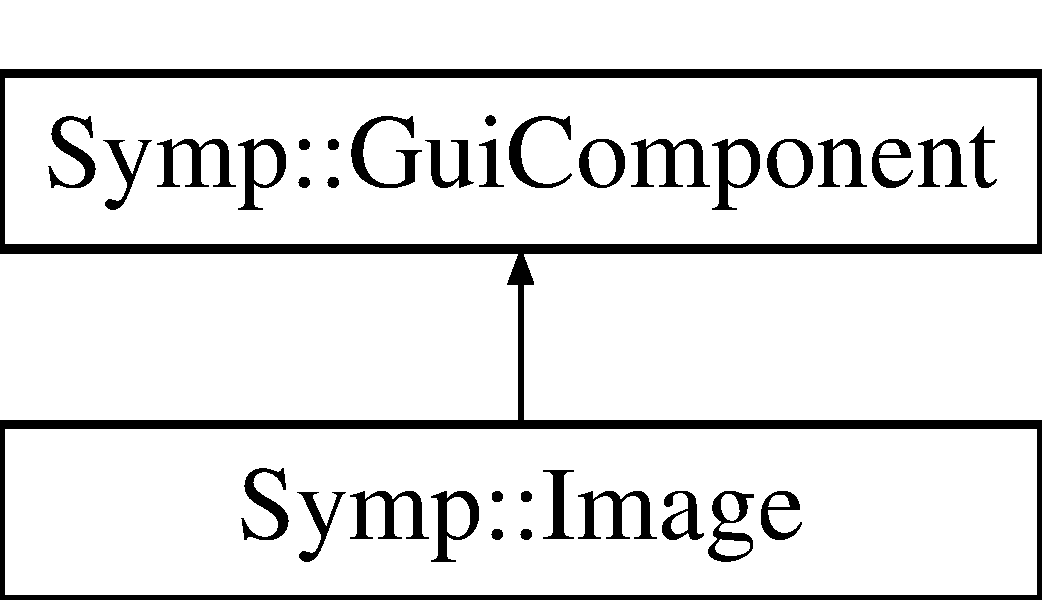
\includegraphics[height=2.000000cm]{class_symp_1_1_image}
\end{center}
\end{figure}
\subsection*{Public Member Functions}
\begin{DoxyCompactItemize}
\item 
\hyperlink{class_symp_1_1_image_afc591fe2f9770e6139509c4c62ffd3c1}{Image} (const char $\ast$file\-Path, float i\-Pos\-X=0, float i\-Pos\-Y=0, float i\-Scale=1.f)
\begin{DoxyCompactList}\small\item\em \hyperlink{class_symp_1_1_image}{Image} class constructor inherits the \hyperlink{class_symp_1_1_gui_component}{Gui\-Component} class Responsible for the initialization of the class private attributes. This constructor will associate a texture to its Indielib I\-N\-D\-\_\-\-Entity2d. The position and scale atributes have default values that can be left for using the \hyperlink{class_symp_1_1_image_afc591fe2f9770e6139509c4c62ffd3c1}{Image} with a \#\-Layout. \end{DoxyCompactList}\item 
\hyperlink{class_symp_1_1_image_a14ac6d979d7c3aed090183e64d42da1d}{$\sim$\-Image} ()
\item 
virtual void \hyperlink{class_symp_1_1_image_a8de69cca37efc613094cfd1311ea1e13}{update} ()
\begin{DoxyCompactList}\small\item\em \hyperlink{class_symp_1_1_image}{Image} update fonction Refresh the display of the \hyperlink{class_symp_1_1_image_afc591fe2f9770e6139509c4c62ffd3c1}{Image}. \end{DoxyCompactList}\item 
void \hyperlink{class_symp_1_1_image_a8546f7d9cb33ce27ecaf13fe18f838ea}{show} ()
\begin{DoxyCompactList}\small\item\em Show the \hyperlink{class_symp_1_1_image}{Image} The \hyperlink{class_symp_1_1_image_a8546f7d9cb33ce27ecaf13fe18f838ea}{show} function doesn't affect attributes of the \hyperlink{class_symp_1_1_image_afc591fe2f9770e6139509c4c62ffd3c1}{Image} class. \end{DoxyCompactList}\item 
void \hyperlink{class_symp_1_1_image_aee4aa4257ba4c4b9d6c7547e2740399e}{hide} ()
\begin{DoxyCompactList}\small\item\em Hide the \hyperlink{class_symp_1_1_image}{Image} The \hyperlink{class_symp_1_1_image_aee4aa4257ba4c4b9d6c7547e2740399e}{hide} function doesn't affect attributes of the \hyperlink{class_symp_1_1_image_afc591fe2f9770e6139509c4c62ffd3c1}{Image} class. \end{DoxyCompactList}\item 
void \hyperlink{class_symp_1_1_image_ac8795b3862086161eaff9047da933456}{fill} (\hyperlink{struct_symp_1_1_color}{Symp\-::\-Color} color)
\begin{DoxyCompactList}\small\item\em fill \hyperlink{class_symp_1_1_image}{Image}'s background function \end{DoxyCompactList}\item 
\hyperlink{namespace_symp_a2d0f7a8e888710a800fc73cf4d1ed38d}{Aspect\-Ratio} \hyperlink{class_symp_1_1_image_a93f4df550738cb50b7edd26dad17bdaf}{get\-Aspect\-Ratio} () const 
\item 
bool \hyperlink{class_symp_1_1_image_a78aa31b99ea41f0fd9cd013b1a34331b}{is\-Shown} () const 
\item 
void \hyperlink{class_symp_1_1_image_affacfb8d2e2dbd24f115b225eeeeed06}{set\-Color} (\hyperlink{struct_symp_1_1_color}{Color} color)
\item 
void \hyperlink{class_symp_1_1_image_aa0a5e8044ba9aa31e64b49dff9ff4218}{set\-Aspect\-Ratio} (\hyperlink{namespace_symp_a2d0f7a8e888710a800fc73cf4d1ed38d}{Aspect\-Ratio} ratio)
\end{DoxyCompactItemize}
\subsection*{Additional Inherited Members}


\subsection{Detailed Description}
This class inherits the \hyperlink{class_symp_1_1_gui_component_a22124675c2976983ac18374f81cc3fb3}{Gui\-Component} class. A \hyperlink{class_symp_1_1_image_afc591fe2f9770e6139509c4c62ffd3c1}{Image} class display a texture. As an \hyperlink{class_symp_1_1_image_afc591fe2f9770e6139509c4c62ffd3c1}{Image} got the inherited parameters of size, the \hyperlink{class_symp_1_1_image_a8de69cca37efc613094cfd1311ea1e13}{update} is made following the type of ratio choosen for the \hyperlink{class_symp_1_1_image_afc591fe2f9770e6139509c4c62ffd3c1}{Image}. The types of ratio are defined in the \hyperlink{namespace_symp_a2d0f7a8e888710a800fc73cf4d1ed38d}{Aspect\-Ratio} enum. The simpliest way to use \hyperlink{class_symp_1_1_image_afc591fe2f9770e6139509c4c62ffd3c1}{Image} is with the \#\-Layout class, that handle the position and the size of the \hyperlink{class_symp_1_1_image_afc591fe2f9770e6139509c4c62ffd3c1}{Image}. of \hyperlink{class_symp_1_1_image_afc591fe2f9770e6139509c4c62ffd3c1}{Image} that will be rendered. \begin{DoxySeeAlso}{See Also}
\hyperlink{class_symp_1_1_menu_manager}{Menu\-Manager} 

\hyperlink{class_symp_1_1_image}{Image} 

\hyperlink{class_symp_1_1_gui_component}{Gui\-Component} 

\hyperlink{class_symp_1_1_layout}{Layout} 
\end{DoxySeeAlso}


Definition at line 33 of file Image.\-h.



\subsection{Constructor \& Destructor Documentation}
\hypertarget{class_symp_1_1_image_afc591fe2f9770e6139509c4c62ffd3c1}{\index{Symp\-::\-Image@{Symp\-::\-Image}!Image@{Image}}
\index{Image@{Image}!Symp::Image@{Symp\-::\-Image}}
\subsubsection[{Image}]{\setlength{\rightskip}{0pt plus 5cm}Symp\-::\-Image\-::\-Image (
\begin{DoxyParamCaption}
\item[{const char $\ast$}]{file\-Path, }
\item[{float}]{i\-Pos\-X = {\ttfamily 0}, }
\item[{float}]{i\-Pos\-Y = {\ttfamily 0}, }
\item[{float}]{i\-Scale = {\ttfamily 1.f}}
\end{DoxyParamCaption}
)}}\label{class_symp_1_1_image_afc591fe2f9770e6139509c4c62ffd3c1}


\hyperlink{class_symp_1_1_image}{Image} class constructor inherits the \hyperlink{class_symp_1_1_gui_component}{Gui\-Component} class Responsible for the initialization of the class private attributes. This constructor will associate a texture to its Indielib I\-N\-D\-\_\-\-Entity2d. The position and scale atributes have default values that can be left for using the \hyperlink{class_symp_1_1_image_afc591fe2f9770e6139509c4c62ffd3c1}{Image} with a \#\-Layout. 


\begin{DoxyParams}{Parameters}
{\em file\-Path} & is the path to the image file \\
\hline
{\em i\-Pos\-X} & the x coordinate of the upper-\/left corner of the \hyperlink{class_symp_1_1_image_afc591fe2f9770e6139509c4c62ffd3c1}{Image} in pixels (default = 0) \\
\hline
{\em i\-Pos\-Y} & the y coordinate of the upper-\/left corner of the \hyperlink{class_symp_1_1_image_afc591fe2f9770e6139509c4c62ffd3c1}{Image} in pixels (default = 0) \\
\hline
{\em i\-Scale} & the uniform scale that will be applied for both width and height between 0 and 1 (default no scale = 1) \\
\hline
\end{DoxyParams}
\begin{DoxySeeAlso}{See Also}
\hyperlink{class_symp_1_1_image}{Image} 

\hyperlink{class_symp_1_1_image_a14ac6d979d7c3aed090183e64d42da1d}{$\sim$\-Image()} 

\hyperlink{class_symp_1_1_gui_component}{Gui\-Component} 
\end{DoxySeeAlso}


Definition at line 21 of file Image.\-cpp.

\hypertarget{class_symp_1_1_image_a14ac6d979d7c3aed090183e64d42da1d}{\index{Symp\-::\-Image@{Symp\-::\-Image}!$\sim$\-Image@{$\sim$\-Image}}
\index{$\sim$\-Image@{$\sim$\-Image}!Symp::Image@{Symp\-::\-Image}}
\subsubsection[{$\sim$\-Image}]{\setlength{\rightskip}{0pt plus 5cm}Symp\-::\-Image\-::$\sim$\-Image (
\begin{DoxyParamCaption}
{}
\end{DoxyParamCaption}
)}}\label{class_symp_1_1_image_a14ac6d979d7c3aed090183e64d42da1d}


\subsection{Member Function Documentation}
\hypertarget{class_symp_1_1_image_ac8795b3862086161eaff9047da933456}{\index{Symp\-::\-Image@{Symp\-::\-Image}!fill@{fill}}
\index{fill@{fill}!Symp::Image@{Symp\-::\-Image}}
\subsubsection[{fill}]{\setlength{\rightskip}{0pt plus 5cm}void Symp\-::\-Image\-::fill (
\begin{DoxyParamCaption}
\item[{{\bf Symp\-::\-Color}}]{color}
\end{DoxyParamCaption}
)}}\label{class_symp_1_1_image_ac8795b3862086161eaff9047da933456}


fill \hyperlink{class_symp_1_1_image}{Image}'s background function 

\begin{DoxySeeAlso}{See Also}
\hyperlink{class_symp_1_1_image}{Image} 

\hyperlink{class_symp_1_1_image_a14ac6d979d7c3aed090183e64d42da1d}{$\sim$\-Image()} 

\hyperlink{struct_symp_1_1_color}{Color} 

\hyperlink{class_symp_1_1_gui_component}{Gui\-Component} 
\end{DoxySeeAlso}


Definition at line 139 of file Image.\-cpp.

\hypertarget{class_symp_1_1_image_a93f4df550738cb50b7edd26dad17bdaf}{\index{Symp\-::\-Image@{Symp\-::\-Image}!get\-Aspect\-Ratio@{get\-Aspect\-Ratio}}
\index{get\-Aspect\-Ratio@{get\-Aspect\-Ratio}!Symp::Image@{Symp\-::\-Image}}
\subsubsection[{get\-Aspect\-Ratio}]{\setlength{\rightskip}{0pt plus 5cm}{\bf Aspect\-Ratio} Symp\-::\-Image\-::get\-Aspect\-Ratio (
\begin{DoxyParamCaption}
{}
\end{DoxyParamCaption}
) const\hspace{0.3cm}{\ttfamily [inline]}}}\label{class_symp_1_1_image_a93f4df550738cb50b7edd26dad17bdaf}


Definition at line 45 of file Image.\-h.

\hypertarget{class_symp_1_1_image_aee4aa4257ba4c4b9d6c7547e2740399e}{\index{Symp\-::\-Image@{Symp\-::\-Image}!hide@{hide}}
\index{hide@{hide}!Symp::Image@{Symp\-::\-Image}}
\subsubsection[{hide}]{\setlength{\rightskip}{0pt plus 5cm}void Symp\-::\-Image\-::hide (
\begin{DoxyParamCaption}
{}
\end{DoxyParamCaption}
)}}\label{class_symp_1_1_image_aee4aa4257ba4c4b9d6c7547e2740399e}


Hide the \hyperlink{class_symp_1_1_image}{Image} The \hyperlink{class_symp_1_1_image_aee4aa4257ba4c4b9d6c7547e2740399e}{hide} function doesn't affect attributes of the \hyperlink{class_symp_1_1_image_afc591fe2f9770e6139509c4c62ffd3c1}{Image} class. 

\begin{DoxySeeAlso}{See Also}
\hyperlink{class_symp_1_1_image}{Image} 

\hyperlink{class_symp_1_1_image_a8546f7d9cb33ce27ecaf13fe18f838ea}{show()} 

\hyperlink{class_symp_1_1_gui_component}{Gui\-Component} 
\end{DoxySeeAlso}


Definition at line 56 of file Image.\-cpp.

\hypertarget{class_symp_1_1_image_a78aa31b99ea41f0fd9cd013b1a34331b}{\index{Symp\-::\-Image@{Symp\-::\-Image}!is\-Shown@{is\-Shown}}
\index{is\-Shown@{is\-Shown}!Symp::Image@{Symp\-::\-Image}}
\subsubsection[{is\-Shown}]{\setlength{\rightskip}{0pt plus 5cm}bool Symp\-::\-Image\-::is\-Shown (
\begin{DoxyParamCaption}
{}
\end{DoxyParamCaption}
) const\hspace{0.3cm}{\ttfamily [inline]}}}\label{class_symp_1_1_image_a78aa31b99ea41f0fd9cd013b1a34331b}


Definition at line 46 of file Image.\-h.

\hypertarget{class_symp_1_1_image_aa0a5e8044ba9aa31e64b49dff9ff4218}{\index{Symp\-::\-Image@{Symp\-::\-Image}!set\-Aspect\-Ratio@{set\-Aspect\-Ratio}}
\index{set\-Aspect\-Ratio@{set\-Aspect\-Ratio}!Symp::Image@{Symp\-::\-Image}}
\subsubsection[{set\-Aspect\-Ratio}]{\setlength{\rightskip}{0pt plus 5cm}void Symp\-::\-Image\-::set\-Aspect\-Ratio (
\begin{DoxyParamCaption}
\item[{{\bf Aspect\-Ratio}}]{ratio}
\end{DoxyParamCaption}
)\hspace{0.3cm}{\ttfamily [inline]}}}\label{class_symp_1_1_image_aa0a5e8044ba9aa31e64b49dff9ff4218}


Definition at line 50 of file Image.\-h.

\hypertarget{class_symp_1_1_image_affacfb8d2e2dbd24f115b225eeeeed06}{\index{Symp\-::\-Image@{Symp\-::\-Image}!set\-Color@{set\-Color}}
\index{set\-Color@{set\-Color}!Symp::Image@{Symp\-::\-Image}}
\subsubsection[{set\-Color}]{\setlength{\rightskip}{0pt plus 5cm}void Symp\-::\-Image\-::set\-Color (
\begin{DoxyParamCaption}
\item[{{\bf Color}}]{color}
\end{DoxyParamCaption}
)\hspace{0.3cm}{\ttfamily [inline]}}}\label{class_symp_1_1_image_affacfb8d2e2dbd24f115b225eeeeed06}


Definition at line 49 of file Image.\-h.

\hypertarget{class_symp_1_1_image_a8546f7d9cb33ce27ecaf13fe18f838ea}{\index{Symp\-::\-Image@{Symp\-::\-Image}!show@{show}}
\index{show@{show}!Symp::Image@{Symp\-::\-Image}}
\subsubsection[{show}]{\setlength{\rightskip}{0pt plus 5cm}void Symp\-::\-Image\-::show (
\begin{DoxyParamCaption}
{}
\end{DoxyParamCaption}
)}}\label{class_symp_1_1_image_a8546f7d9cb33ce27ecaf13fe18f838ea}


Show the \hyperlink{class_symp_1_1_image}{Image} The \hyperlink{class_symp_1_1_image_a8546f7d9cb33ce27ecaf13fe18f838ea}{show} function doesn't affect attributes of the \hyperlink{class_symp_1_1_image_afc591fe2f9770e6139509c4c62ffd3c1}{Image} class. 

\begin{DoxySeeAlso}{See Also}
\hyperlink{class_symp_1_1_image}{Image} 

\hyperlink{class_symp_1_1_image_aee4aa4257ba4c4b9d6c7547e2740399e}{hide()} 

\hyperlink{class_symp_1_1_gui_component}{Gui\-Component} 
\end{DoxySeeAlso}


Definition at line 45 of file Image.\-cpp.

\hypertarget{class_symp_1_1_image_a8de69cca37efc613094cfd1311ea1e13}{\index{Symp\-::\-Image@{Symp\-::\-Image}!update@{update}}
\index{update@{update}!Symp::Image@{Symp\-::\-Image}}
\subsubsection[{update}]{\setlength{\rightskip}{0pt plus 5cm}void Symp\-::\-Image\-::update (
\begin{DoxyParamCaption}
{}
\end{DoxyParamCaption}
)\hspace{0.3cm}{\ttfamily [virtual]}}}\label{class_symp_1_1_image_a8de69cca37efc613094cfd1311ea1e13}


\hyperlink{class_symp_1_1_image}{Image} update fonction Refresh the display of the \hyperlink{class_symp_1_1_image_afc591fe2f9770e6139509c4c62ffd3c1}{Image}. 

\begin{DoxySeeAlso}{See Also}
\hyperlink{class_symp_1_1_image}{Image} 

\hyperlink{class_symp_1_1_image_a14ac6d979d7c3aed090183e64d42da1d}{$\sim$\-Image()} 

\hyperlink{class_symp_1_1_gui_component}{Gui\-Component} 
\end{DoxySeeAlso}


Implements \hyperlink{class_symp_1_1_gui_component_add73e07ea0a3c9c1c90640e783a3b5de}{Symp\-::\-Gui\-Component}.



Definition at line 68 of file Image.\-cpp.



The documentation for this class was generated from the following files\-:\begin{DoxyCompactItemize}
\item 
/home/cecilia/\-Documents/\-Symptogen/src/menu/\hyperlink{_image_8h}{Image.\-h}\item 
/home/cecilia/\-Documents/\-Symptogen/src/menu/\hyperlink{_image_8cpp}{Image.\-cpp}\end{DoxyCompactItemize}

\hypertarget{class_symp_1_1_input_manager}{\section{Symp\-:\-:Input\-Manager Class Reference}
\label{class_symp_1_1_input_manager}\index{Symp\-::\-Input\-Manager@{Symp\-::\-Input\-Manager}}
}


{\ttfamily \#include $<$Input\-Manager.\-h$>$}

Inheritance diagram for Symp\-:\-:Input\-Manager\-:\begin{figure}[H]
\begin{center}
\leavevmode
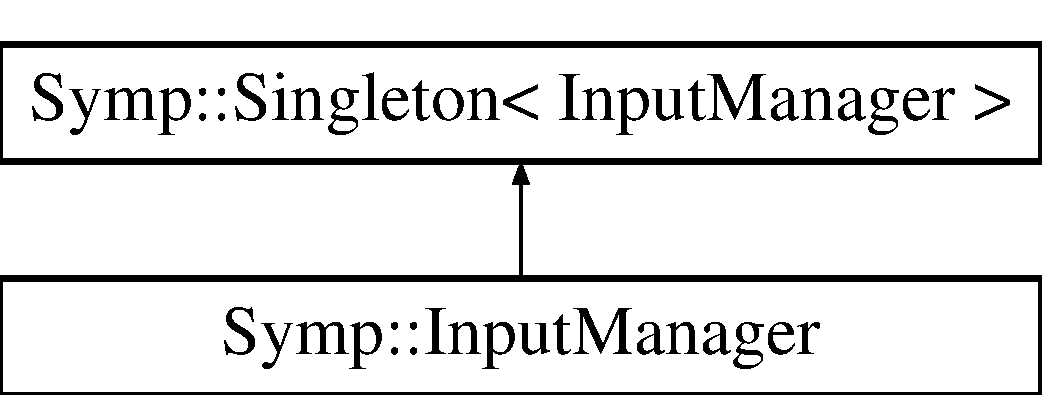
\includegraphics[height=2.000000cm]{class_symp_1_1_input_manager}
\end{center}
\end{figure}
\subsection*{Public Member Functions}
\begin{DoxyCompactItemize}
\item 
void \hyperlink{class_symp_1_1_input_manager_a4b0de18e7d9db24f0f23206ab6868c78}{init\-Render} (\hyperlink{class_symp_1_1_render}{Render} $\ast$p\-Render)
\item 
void \hyperlink{class_symp_1_1_input_manager_a17e5bde3349c5acfdcaed337606f2006}{update} ()
\item 
bool \hyperlink{class_symp_1_1_input_manager_a686f69d4eeba6aa7b1072da8ac542e97}{quit} ()
\item 
bool \hyperlink{class_symp_1_1_input_manager_ab64961cda313a90023bb69fe238290ec}{on\-Key\-Press} (I\-N\-D\-\_\-\-Key p\-Key)
\item 
bool \hyperlink{class_symp_1_1_input_manager_a9766fbfc17a36de3f66232a712903c4e}{on\-Key\-Release} (I\-N\-D\-\_\-\-Key p\-Key)
\item 
bool \hyperlink{class_symp_1_1_input_manager_a0c7312f32732c5a4bf678ec3fdbf8ec0}{is\-Key\-Pressed} (I\-N\-D\-\_\-\-Key p\-Key)
\item 
bool \hyperlink{class_symp_1_1_input_manager_a46c0e5311522ed10818726f4b553a273}{is\-Key\-Pressed} (I\-N\-D\-\_\-\-Key p\-Key, unsigned long p\-Time)
\item 
int \hyperlink{class_symp_1_1_input_manager_a98a0e230497375792f0f3f0e4193b877}{get\-Mouse\-X} ()
\item 
int \hyperlink{class_symp_1_1_input_manager_a74d8c0805e2c35342bae7372cfa25eb9}{get\-Mouse\-Y} ()
\item 
bool \hyperlink{class_symp_1_1_input_manager_a1d165f8b05abd4917b80057b8dcc1b57}{is\-Mouse\-Motion} ()
\item 
bool \hyperlink{class_symp_1_1_input_manager_a59ae59e4026ec437e30ac1338a1b4d57}{on\-Mouse\-Button\-Press} (I\-N\-D\-\_\-\-Mouse\-Button p\-Mouse\-Button)
\item 
bool \hyperlink{class_symp_1_1_input_manager_a16fb8eea2121bc783bf4802ce6331452}{on\-Mouse\-Button\-Release} (I\-N\-D\-\_\-\-Mouse\-Button p\-Mouse\-Button)
\item 
bool \hyperlink{class_symp_1_1_input_manager_a328f07308b781f78c937354f0e85fe89}{is\-Mouse\-Button\-Pressed} (I\-N\-D\-\_\-\-Mouse\-Button p\-Mouse\-Button)
\item 
bool \hyperlink{class_symp_1_1_input_manager_a364ae17c2627897c66f51e29fca289b2}{is\-Mouse\-Button\-Pressed} (I\-N\-D\-\_\-\-Mouse\-Button p\-Mouse\-Button, unsigned long p\-Time)
\item 
I\-N\-D\-\_\-\-Input $\ast$ \hyperlink{class_symp_1_1_input_manager_a1c42a4ed489d11686b164d81dc25eb9e}{get\-I\-N\-D\-\_\-\-Input} ()
\end{DoxyCompactItemize}
\subsection*{Friends}
\begin{DoxyCompactItemize}
\item 
class \hyperlink{class_symp_1_1_input_manager_a66d11072af334ea886589fb16a08df50}{Singleton$<$ Input\-Manager $>$}
\end{DoxyCompactItemize}
\subsection*{Additional Inherited Members}


\subsection{Detailed Description}
Facade of I\-N\-D\-\_\-\-Input. 

Definition at line 15 of file Input\-Manager.\-h.



\subsection{Member Function Documentation}
\hypertarget{class_symp_1_1_input_manager_a1c42a4ed489d11686b164d81dc25eb9e}{\index{Symp\-::\-Input\-Manager@{Symp\-::\-Input\-Manager}!get\-I\-N\-D\-\_\-\-Input@{get\-I\-N\-D\-\_\-\-Input}}
\index{get\-I\-N\-D\-\_\-\-Input@{get\-I\-N\-D\-\_\-\-Input}!Symp::InputManager@{Symp\-::\-Input\-Manager}}
\subsubsection[{get\-I\-N\-D\-\_\-\-Input}]{\setlength{\rightskip}{0pt plus 5cm}I\-N\-D\-\_\-\-Input$\ast$ Symp\-::\-Input\-Manager\-::get\-I\-N\-D\-\_\-\-Input (
\begin{DoxyParamCaption}
{}
\end{DoxyParamCaption}
)\hspace{0.3cm}{\ttfamily [inline]}}}\label{class_symp_1_1_input_manager_a1c42a4ed489d11686b164d81dc25eb9e}


Definition at line 41 of file Input\-Manager.\-h.

\hypertarget{class_symp_1_1_input_manager_a98a0e230497375792f0f3f0e4193b877}{\index{Symp\-::\-Input\-Manager@{Symp\-::\-Input\-Manager}!get\-Mouse\-X@{get\-Mouse\-X}}
\index{get\-Mouse\-X@{get\-Mouse\-X}!Symp::InputManager@{Symp\-::\-Input\-Manager}}
\subsubsection[{get\-Mouse\-X}]{\setlength{\rightskip}{0pt plus 5cm}int Symp\-::\-Input\-Manager\-::get\-Mouse\-X (
\begin{DoxyParamCaption}
{}
\end{DoxyParamCaption}
)}}\label{class_symp_1_1_input_manager_a98a0e230497375792f0f3f0e4193b877}


Definition at line 61 of file Input\-Manager.\-cpp.

\hypertarget{class_symp_1_1_input_manager_a74d8c0805e2c35342bae7372cfa25eb9}{\index{Symp\-::\-Input\-Manager@{Symp\-::\-Input\-Manager}!get\-Mouse\-Y@{get\-Mouse\-Y}}
\index{get\-Mouse\-Y@{get\-Mouse\-Y}!Symp::InputManager@{Symp\-::\-Input\-Manager}}
\subsubsection[{get\-Mouse\-Y}]{\setlength{\rightskip}{0pt plus 5cm}int Symp\-::\-Input\-Manager\-::get\-Mouse\-Y (
\begin{DoxyParamCaption}
{}
\end{DoxyParamCaption}
)}}\label{class_symp_1_1_input_manager_a74d8c0805e2c35342bae7372cfa25eb9}


Definition at line 65 of file Input\-Manager.\-cpp.

\hypertarget{class_symp_1_1_input_manager_a4b0de18e7d9db24f0f23206ab6868c78}{\index{Symp\-::\-Input\-Manager@{Symp\-::\-Input\-Manager}!init\-Render@{init\-Render}}
\index{init\-Render@{init\-Render}!Symp::InputManager@{Symp\-::\-Input\-Manager}}
\subsubsection[{init\-Render}]{\setlength{\rightskip}{0pt plus 5cm}void Symp\-::\-Input\-Manager\-::init\-Render (
\begin{DoxyParamCaption}
\item[{{\bf Render} $\ast$}]{p\-Render}
\end{DoxyParamCaption}
)}}\label{class_symp_1_1_input_manager_a4b0de18e7d9db24f0f23206ab6868c78}


Definition at line 14 of file Input\-Manager.\-cpp.

\hypertarget{class_symp_1_1_input_manager_a0c7312f32732c5a4bf678ec3fdbf8ec0}{\index{Symp\-::\-Input\-Manager@{Symp\-::\-Input\-Manager}!is\-Key\-Pressed@{is\-Key\-Pressed}}
\index{is\-Key\-Pressed@{is\-Key\-Pressed}!Symp::InputManager@{Symp\-::\-Input\-Manager}}
\subsubsection[{is\-Key\-Pressed}]{\setlength{\rightskip}{0pt plus 5cm}bool Symp\-::\-Input\-Manager\-::is\-Key\-Pressed (
\begin{DoxyParamCaption}
\item[{I\-N\-D\-\_\-\-Key}]{p\-Key}
\end{DoxyParamCaption}
)}}\label{class_symp_1_1_input_manager_a0c7312f32732c5a4bf678ec3fdbf8ec0}


Definition at line 34 of file Input\-Manager.\-cpp.

\hypertarget{class_symp_1_1_input_manager_a46c0e5311522ed10818726f4b553a273}{\index{Symp\-::\-Input\-Manager@{Symp\-::\-Input\-Manager}!is\-Key\-Pressed@{is\-Key\-Pressed}}
\index{is\-Key\-Pressed@{is\-Key\-Pressed}!Symp::InputManager@{Symp\-::\-Input\-Manager}}
\subsubsection[{is\-Key\-Pressed}]{\setlength{\rightskip}{0pt plus 5cm}bool Symp\-::\-Input\-Manager\-::is\-Key\-Pressed (
\begin{DoxyParamCaption}
\item[{I\-N\-D\-\_\-\-Key}]{p\-Key, }
\item[{unsigned long}]{p\-Time}
\end{DoxyParamCaption}
)}}\label{class_symp_1_1_input_manager_a46c0e5311522ed10818726f4b553a273}


Definition at line 38 of file Input\-Manager.\-cpp.

\hypertarget{class_symp_1_1_input_manager_a328f07308b781f78c937354f0e85fe89}{\index{Symp\-::\-Input\-Manager@{Symp\-::\-Input\-Manager}!is\-Mouse\-Button\-Pressed@{is\-Mouse\-Button\-Pressed}}
\index{is\-Mouse\-Button\-Pressed@{is\-Mouse\-Button\-Pressed}!Symp::InputManager@{Symp\-::\-Input\-Manager}}
\subsubsection[{is\-Mouse\-Button\-Pressed}]{\setlength{\rightskip}{0pt plus 5cm}bool Symp\-::\-Input\-Manager\-::is\-Mouse\-Button\-Pressed (
\begin{DoxyParamCaption}
\item[{I\-N\-D\-\_\-\-Mouse\-Button}]{p\-Mouse\-Button}
\end{DoxyParamCaption}
)}}\label{class_symp_1_1_input_manager_a328f07308b781f78c937354f0e85fe89}


Definition at line 53 of file Input\-Manager.\-cpp.

\hypertarget{class_symp_1_1_input_manager_a364ae17c2627897c66f51e29fca289b2}{\index{Symp\-::\-Input\-Manager@{Symp\-::\-Input\-Manager}!is\-Mouse\-Button\-Pressed@{is\-Mouse\-Button\-Pressed}}
\index{is\-Mouse\-Button\-Pressed@{is\-Mouse\-Button\-Pressed}!Symp::InputManager@{Symp\-::\-Input\-Manager}}
\subsubsection[{is\-Mouse\-Button\-Pressed}]{\setlength{\rightskip}{0pt plus 5cm}bool Symp\-::\-Input\-Manager\-::is\-Mouse\-Button\-Pressed (
\begin{DoxyParamCaption}
\item[{I\-N\-D\-\_\-\-Mouse\-Button}]{p\-Mouse\-Button, }
\item[{unsigned long}]{p\-Time}
\end{DoxyParamCaption}
)}}\label{class_symp_1_1_input_manager_a364ae17c2627897c66f51e29fca289b2}


Definition at line 57 of file Input\-Manager.\-cpp.

\hypertarget{class_symp_1_1_input_manager_a1d165f8b05abd4917b80057b8dcc1b57}{\index{Symp\-::\-Input\-Manager@{Symp\-::\-Input\-Manager}!is\-Mouse\-Motion@{is\-Mouse\-Motion}}
\index{is\-Mouse\-Motion@{is\-Mouse\-Motion}!Symp::InputManager@{Symp\-::\-Input\-Manager}}
\subsubsection[{is\-Mouse\-Motion}]{\setlength{\rightskip}{0pt plus 5cm}bool Symp\-::\-Input\-Manager\-::is\-Mouse\-Motion (
\begin{DoxyParamCaption}
{}
\end{DoxyParamCaption}
)}}\label{class_symp_1_1_input_manager_a1d165f8b05abd4917b80057b8dcc1b57}


Definition at line 41 of file Input\-Manager.\-cpp.

\hypertarget{class_symp_1_1_input_manager_ab64961cda313a90023bb69fe238290ec}{\index{Symp\-::\-Input\-Manager@{Symp\-::\-Input\-Manager}!on\-Key\-Press@{on\-Key\-Press}}
\index{on\-Key\-Press@{on\-Key\-Press}!Symp::InputManager@{Symp\-::\-Input\-Manager}}
\subsubsection[{on\-Key\-Press}]{\setlength{\rightskip}{0pt plus 5cm}bool Symp\-::\-Input\-Manager\-::on\-Key\-Press (
\begin{DoxyParamCaption}
\item[{I\-N\-D\-\_\-\-Key}]{p\-Key}
\end{DoxyParamCaption}
)}}\label{class_symp_1_1_input_manager_ab64961cda313a90023bb69fe238290ec}


Definition at line 26 of file Input\-Manager.\-cpp.

\hypertarget{class_symp_1_1_input_manager_a9766fbfc17a36de3f66232a712903c4e}{\index{Symp\-::\-Input\-Manager@{Symp\-::\-Input\-Manager}!on\-Key\-Release@{on\-Key\-Release}}
\index{on\-Key\-Release@{on\-Key\-Release}!Symp::InputManager@{Symp\-::\-Input\-Manager}}
\subsubsection[{on\-Key\-Release}]{\setlength{\rightskip}{0pt plus 5cm}bool Symp\-::\-Input\-Manager\-::on\-Key\-Release (
\begin{DoxyParamCaption}
\item[{I\-N\-D\-\_\-\-Key}]{p\-Key}
\end{DoxyParamCaption}
)}}\label{class_symp_1_1_input_manager_a9766fbfc17a36de3f66232a712903c4e}


Definition at line 30 of file Input\-Manager.\-cpp.

\hypertarget{class_symp_1_1_input_manager_a59ae59e4026ec437e30ac1338a1b4d57}{\index{Symp\-::\-Input\-Manager@{Symp\-::\-Input\-Manager}!on\-Mouse\-Button\-Press@{on\-Mouse\-Button\-Press}}
\index{on\-Mouse\-Button\-Press@{on\-Mouse\-Button\-Press}!Symp::InputManager@{Symp\-::\-Input\-Manager}}
\subsubsection[{on\-Mouse\-Button\-Press}]{\setlength{\rightskip}{0pt plus 5cm}bool Symp\-::\-Input\-Manager\-::on\-Mouse\-Button\-Press (
\begin{DoxyParamCaption}
\item[{I\-N\-D\-\_\-\-Mouse\-Button}]{p\-Mouse\-Button}
\end{DoxyParamCaption}
)}}\label{class_symp_1_1_input_manager_a59ae59e4026ec437e30ac1338a1b4d57}


Definition at line 45 of file Input\-Manager.\-cpp.

\hypertarget{class_symp_1_1_input_manager_a16fb8eea2121bc783bf4802ce6331452}{\index{Symp\-::\-Input\-Manager@{Symp\-::\-Input\-Manager}!on\-Mouse\-Button\-Release@{on\-Mouse\-Button\-Release}}
\index{on\-Mouse\-Button\-Release@{on\-Mouse\-Button\-Release}!Symp::InputManager@{Symp\-::\-Input\-Manager}}
\subsubsection[{on\-Mouse\-Button\-Release}]{\setlength{\rightskip}{0pt plus 5cm}bool Symp\-::\-Input\-Manager\-::on\-Mouse\-Button\-Release (
\begin{DoxyParamCaption}
\item[{I\-N\-D\-\_\-\-Mouse\-Button}]{p\-Mouse\-Button}
\end{DoxyParamCaption}
)}}\label{class_symp_1_1_input_manager_a16fb8eea2121bc783bf4802ce6331452}


Definition at line 49 of file Input\-Manager.\-cpp.

\hypertarget{class_symp_1_1_input_manager_a686f69d4eeba6aa7b1072da8ac542e97}{\index{Symp\-::\-Input\-Manager@{Symp\-::\-Input\-Manager}!quit@{quit}}
\index{quit@{quit}!Symp::InputManager@{Symp\-::\-Input\-Manager}}
\subsubsection[{quit}]{\setlength{\rightskip}{0pt plus 5cm}bool Symp\-::\-Input\-Manager\-::quit (
\begin{DoxyParamCaption}
{}
\end{DoxyParamCaption}
)}}\label{class_symp_1_1_input_manager_a686f69d4eeba6aa7b1072da8ac542e97}


Definition at line 22 of file Input\-Manager.\-cpp.

\hypertarget{class_symp_1_1_input_manager_a17e5bde3349c5acfdcaed337606f2006}{\index{Symp\-::\-Input\-Manager@{Symp\-::\-Input\-Manager}!update@{update}}
\index{update@{update}!Symp::InputManager@{Symp\-::\-Input\-Manager}}
\subsubsection[{update}]{\setlength{\rightskip}{0pt plus 5cm}void Symp\-::\-Input\-Manager\-::update (
\begin{DoxyParamCaption}
{}
\end{DoxyParamCaption}
)}}\label{class_symp_1_1_input_manager_a17e5bde3349c5acfdcaed337606f2006}


Definition at line 18 of file Input\-Manager.\-cpp.



\subsection{Friends And Related Function Documentation}
\hypertarget{class_symp_1_1_input_manager_a66d11072af334ea886589fb16a08df50}{\index{Symp\-::\-Input\-Manager@{Symp\-::\-Input\-Manager}!Singleton$<$ Input\-Manager $>$@{Singleton$<$ Input\-Manager $>$}}
\index{Singleton$<$ Input\-Manager $>$@{Singleton$<$ Input\-Manager $>$}!Symp::InputManager@{Symp\-::\-Input\-Manager}}
\subsubsection[{Singleton$<$ Input\-Manager $>$}]{\setlength{\rightskip}{0pt plus 5cm}friend class {\bf Singleton}$<$ {\bf Input\-Manager} $>$\hspace{0.3cm}{\ttfamily [friend]}}}\label{class_symp_1_1_input_manager_a66d11072af334ea886589fb16a08df50}


Definition at line 18 of file Input\-Manager.\-h.



The documentation for this class was generated from the following files\-:\begin{DoxyCompactItemize}
\item 
/home/cecilia/\-Documents/\-Symptogen/src/input/\hyperlink{_input_manager_8h}{Input\-Manager.\-h}\item 
/home/cecilia/\-Documents/\-Symptogen/src/input/\hyperlink{_input_manager_8cpp}{Input\-Manager.\-cpp}\end{DoxyCompactItemize}

\hypertarget{class_interface}{\section{Interface Class Reference}
\label{class_interface}\index{Interface@{Interface}}
}


\subsection{Detailed Description}
class is part of the State Machine pattern that implements the menus management. Each menu inherits State class to be managed by the Menu\-Manager. \begin{DoxySeeAlso}{See Also}
Menu\-Manager 
\end{DoxySeeAlso}


Definition at line 9 of file State.\-h.



The documentation for this class was generated from the following file\-:\begin{DoxyCompactItemize}
\item 
/home/cecilia/\-Documents/\-Symptogen/src/menu/\hyperlink{_state_8h}{State.\-h}\end{DoxyCompactItemize}

\hypertarget{class_symp_1_1_layout}{\section{Symp\-:\-:Layout Class Reference}
\label{class_symp_1_1_layout}\index{Symp\-::\-Layout@{Symp\-::\-Layout}}
}


{\ttfamily \#include $<$Layout.\-h$>$}

Inheritance diagram for Symp\-:\-:Layout\-:\begin{figure}[H]
\begin{center}
\leavevmode
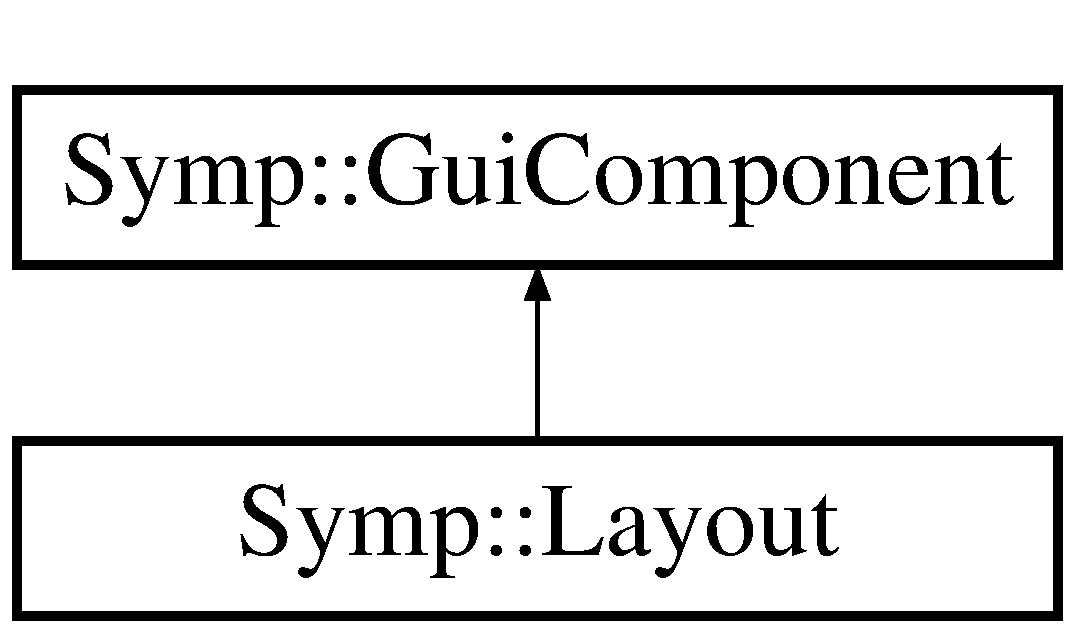
\includegraphics[height=2.000000cm]{class_symp_1_1_layout}
\end{center}
\end{figure}
\subsection*{Public Member Functions}
\begin{DoxyCompactItemize}
\item 
\hyperlink{class_symp_1_1_layout_acd02d4152c342a37567cbbdcec57814f}{Layout} ()
\begin{DoxyCompactList}\small\item\em \hyperlink{class_symp_1_1_layout}{Layout} constructor Responsible for the initialization of the private attributes of \hyperlink{class_symp_1_1_layout_acd02d4152c342a37567cbbdcec57814f}{Layout} class. This simple constructor is meant to be used in the case you want to add a \hyperlink{class_symp_1_1_layout_acd02d4152c342a37567cbbdcec57814f}{Layout} in an other \hyperlink{class_symp_1_1_layout_acd02d4152c342a37567cbbdcec57814f}{Layout}, so the \hyperlink{class_symp_1_1_layout_acd02d4152c342a37567cbbdcec57814f}{Layout} container will manage this \hyperlink{class_symp_1_1_layout_acd02d4152c342a37567cbbdcec57814f}{Layout} size and position. \end{DoxyCompactList}\item 
\hyperlink{class_symp_1_1_layout_a5aa32fa1772ee96bd36432a78bc69aaa}{Layout} (float i\-Pos\-X, float i\-Pos\-Y, int i\-Width, int i\-Height, \hyperlink{struct_symp_1_1_color}{Color} color=\hyperlink{struct_symp_1_1_color}{Color}(0, 0, 0), \hyperlink{namespace_symp_a30499696a7501e2c08fdf0b3094484fb}{Layout\-Fill\-Attribute} fill\-Attribute=Layout\-Fill\-Attribute\-::\-N\-O\-N\-E)
\begin{DoxyCompactList}\small\item\em \hyperlink{class_symp_1_1_layout}{Layout} constructor Responsible for the initialization of the private attributes of \hyperlink{class_symp_1_1_layout_acd02d4152c342a37567cbbdcec57814f}{Layout} class. This is the complete version of the \hyperlink{class_symp_1_1_layout_acd02d4152c342a37567cbbdcec57814f}{Layout} constructor. If this \hyperlink{class_symp_1_1_layout_acd02d4152c342a37567cbbdcec57814f}{Layout} is meant to be used in an other \hyperlink{class_symp_1_1_layout_acd02d4152c342a37567cbbdcec57814f}{Layout}, please use the simple constructor instead of this one. \end{DoxyCompactList}\item 
\hyperlink{class_symp_1_1_layout_a87402d517389b707ccc4cdbb06645ea5}{$\sim$\-Layout} ()
\item 
virtual void \hyperlink{class_symp_1_1_layout_a34a3df4f1637d1a95015e19a1ecf7fb4}{update} ()
\item 
void \hyperlink{class_symp_1_1_layout_a86daa8cdec516e9d469dc09ca2e2c3d6}{add\-Component} (\hyperlink{class_symp_1_1_gui_component}{Gui\-Component} $\ast$p\-Component, int column, int row, bool b\-Resizable=true)
\begin{DoxyCompactList}\small\item\em Add a \hyperlink{class_symp_1_1_gui_component_a22124675c2976983ac18374f81cc3fb3}{Gui\-Component} into the grid to the given row and column indexes When a new component is added to the grid, the grid is re-\/computed and all the components are updated to the new standard component's size. When a \hyperlink{class_symp_1_1_gui_component_a22124675c2976983ac18374f81cc3fb3}{Gui\-Component} is added to a \hyperlink{class_symp_1_1_layout_acd02d4152c342a37567cbbdcec57814f}{Layout}, there is no need to render it to also add the \hyperlink{class_symp_1_1_gui_component_a22124675c2976983ac18374f81cc3fb3}{Gui\-Component} to the \#\-Menu\-Manager \-: the \hyperlink{class_symp_1_1_layout_acd02d4152c342a37567cbbdcec57814f}{Layout} is responsible of adding its components to the \#\-Menu\-Manager. If the \hyperlink{class_symp_1_1_gui_component_a22124675c2976983ac18374f81cc3fb3}{Gui\-Component} is added to the \hyperlink{class_symp_1_1_layout_acd02d4152c342a37567cbbdcec57814f}{Layout} with no need to manage its size and its position, them the attribute resizable need to be set to false, so the grid will not manage this component, true by default. \end{DoxyCompactList}\item 
void \hyperlink{class_symp_1_1_layout_a09bfa1d705aa85fdc81d8b38a871af32}{fill} (\hyperlink{struct_symp_1_1_color}{Symp\-::\-Color} color)
\begin{DoxyCompactList}\small\item\em fill \hyperlink{class_symp_1_1_layout_acd02d4152c342a37567cbbdcec57814f}{Layout}'s background or border following the \hyperlink{namespace_symp_a30499696a7501e2c08fdf0b3094484fb}{Layout\-Fill\-Attribute} \end{DoxyCompactList}\item 
void \hyperlink{class_symp_1_1_layout_a915da50f7032eb8823f86e326ee57ec1}{insert\-Space} (int i\-Column, int i\-Row)
\begin{DoxyCompactList}\small\item\em Insert a blanck space the size of a standard grid component into the \hyperlink{class_symp_1_1_layout_acd02d4152c342a37567cbbdcec57814f}{Layout} grid It is possible to add a space wherever into the grid, but its size as every component of the grid will be standard. \end{DoxyCompactList}\item 
void \hyperlink{class_symp_1_1_layout_a5ccafed047774ddb69c6e87480ae74ee}{compute\-Grid} (int i\-Column, int i\-Row)
\begin{DoxyCompactList}\small\item\em Compute the characteristic of the \hyperlink{class_symp_1_1_layout_acd02d4152c342a37567cbbdcec57814f}{Layout} grid Given a couple of column / row indexes reference, if they are non existing yet, this function determine the standard size of a \hyperlink{class_symp_1_1_gui_component_a22124675c2976983ac18374f81cc3fb3}{Gui\-Component} into the grid. This function is called whenever a \hyperlink{class_symp_1_1_gui_component_a22124675c2976983ac18374f81cc3fb3}{Gui\-Component} is added to the grid. The couple column/row is the position of the \hyperlink{class_symp_1_1_gui_component_a22124675c2976983ac18374f81cc3fb3}{Gui\-Component}, so if a component is placed in a new column or in a new row, the grid adjusts itself and all the components in it. \end{DoxyCompactList}\item 
void \hyperlink{class_symp_1_1_layout_ab6f730d068d35ee75672ced8d06051a4}{resize\-Components} ()
\begin{DoxyCompactList}\small\item\em Resize one by one the \hyperlink{class_symp_1_1_gui_component_a22124675c2976983ac18374f81cc3fb3}{Gui\-Component} contained in the \hyperlink{class_symp_1_1_layout_acd02d4152c342a37567cbbdcec57814f}{Layout} grid Using the reference width and height calculated by the \hyperlink{class_symp_1_1_layout_a5ccafed047774ddb69c6e87480ae74ee}{compute\-Grid()} function, this function retrieve the \hyperlink{class_symp_1_1_gui_component_a22124675c2976983ac18374f81cc3fb3}{Gui\-Component} of the \hyperlink{class_symp_1_1_layout_acd02d4152c342a37567cbbdcec57814f}{Layout} and following their position in the grid, update them with the right size and position. \end{DoxyCompactList}\item 
int \hyperlink{class_symp_1_1_layout_a5a7d9879416e1fb408d76f371c878f16}{get\-Vertical\-Margin} () const 
\item 
int \hyperlink{class_symp_1_1_layout_a612d289b9e6b1300a56cbe5c5ccc6dd8}{get\-Horizontal\-Margin} () const 
\item 
std\-::vector$<$ \hyperlink{class_symp_1_1_gui_component}{Gui\-Component} $\ast$ $>$ \hyperlink{class_symp_1_1_layout_a2a0e436be7c12e5c4d4854d2a86629a5}{get\-Components} () const 
\item 
void \hyperlink{class_symp_1_1_layout_a41abf7a0cabb0ccd6de59a14f78c1916}{set\-Horizontal\-Margin} (int i\-Margin)
\item 
void \hyperlink{class_symp_1_1_layout_ae9c9d682a5ed31a7ca80136d365f249e}{set\-Vertical\-Margin} (int i\-Margin)
\item 
void \hyperlink{class_symp_1_1_layout_a6f50ff9c6d911ff688bfe86125f11c60}{set\-Margins} (int i\-Margin)
\end{DoxyCompactItemize}
\subsection*{Additional Inherited Members}


\subsection{Detailed Description}
the \hyperlink{class_symp_1_1_gui_component_a22124675c2976983ac18374f81cc3fb3}{Gui\-Component} class The \hyperlink{class_symp_1_1_layout_acd02d4152c342a37567cbbdcec57814f}{Layout} class is part of the menu graphical components and can be used only in the menu context. A \hyperlink{class_symp_1_1_layout_acd02d4152c342a37567cbbdcec57814f}{Layout} is meant to group other \#\-Gui\-Components and to organize their display in a regular grid. It is possible to use the \hyperlink{class_symp_1_1_layout_acd02d4152c342a37567cbbdcec57814f}{Layout} to group \hyperlink{class_symp_1_1_gui_component_a22124675c2976983ac18374f81cc3fb3}{Gui\-Component} and to manually set the components position, without organizing them automatically into a grid. A \hyperlink{class_symp_1_1_layout_acd02d4152c342a37567cbbdcec57814f}{Layout} can be cutomized following the \hyperlink{namespace_symp_a30499696a7501e2c08fdf0b3094484fb}{Layout\-Fill\-Attribute}. As every \hyperlink{class_symp_1_1_gui_component_a22124675c2976983ac18374f81cc3fb3}{Gui\-Component}, to be displayed, the \hyperlink{class_symp_1_1_layout_acd02d4152c342a37567cbbdcec57814f}{Layout} must be added to the \#\-Menu\-Manager. Moreover, a \hyperlink{class_symp_1_1_layout_acd02d4152c342a37567cbbdcec57814f}{Layout} automatically add its components to the \#\-Menu\-Manager. A \hyperlink{class_symp_1_1_layout_acd02d4152c342a37567cbbdcec57814f}{Layout} can contain other \hyperlink{class_symp_1_1_layout_acd02d4152c342a37567cbbdcec57814f}{Layout} and manage them as if they are simple \hyperlink{class_symp_1_1_gui_component_a22124675c2976983ac18374f81cc3fb3}{Gui\-Component}. \begin{DoxySeeAlso}{See Also}
\hyperlink{class_symp_1_1_menu_manager}{Menu\-Manager} 

\hyperlink{class_symp_1_1_gui_component}{Gui\-Component} 

\hyperlink{namespace_symp_a30499696a7501e2c08fdf0b3094484fb}{Layout\-Fill\-Attribute} 

\hyperlink{class_symp_1_1_layout_acd02d4152c342a37567cbbdcec57814f}{Layout()} 

\hyperlink{class_symp_1_1_layout_a87402d517389b707ccc4cdbb06645ea5}{$\sim$\-Layout()} 
\end{DoxySeeAlso}


Definition at line 40 of file Layout.\-h.



\subsection{Constructor \& Destructor Documentation}
\hypertarget{class_symp_1_1_layout_acd02d4152c342a37567cbbdcec57814f}{\index{Symp\-::\-Layout@{Symp\-::\-Layout}!Layout@{Layout}}
\index{Layout@{Layout}!Symp::Layout@{Symp\-::\-Layout}}
\subsubsection[{Layout}]{\setlength{\rightskip}{0pt plus 5cm}Symp\-::\-Layout\-::\-Layout (
\begin{DoxyParamCaption}
{}
\end{DoxyParamCaption}
)}}\label{class_symp_1_1_layout_acd02d4152c342a37567cbbdcec57814f}


\hyperlink{class_symp_1_1_layout}{Layout} constructor Responsible for the initialization of the private attributes of \hyperlink{class_symp_1_1_layout_acd02d4152c342a37567cbbdcec57814f}{Layout} class. This simple constructor is meant to be used in the case you want to add a \hyperlink{class_symp_1_1_layout_acd02d4152c342a37567cbbdcec57814f}{Layout} in an other \hyperlink{class_symp_1_1_layout_acd02d4152c342a37567cbbdcec57814f}{Layout}, so the \hyperlink{class_symp_1_1_layout_acd02d4152c342a37567cbbdcec57814f}{Layout} container will manage this \hyperlink{class_symp_1_1_layout_acd02d4152c342a37567cbbdcec57814f}{Layout} size and position. 

\begin{DoxySeeAlso}{See Also}
\hyperlink{struct_symp_1_1_color}{Color} 

\hyperlink{class_symp_1_1_gui_component}{Gui\-Component} 

\hyperlink{class_symp_1_1_layout}{Layout} 

\hyperlink{class_symp_1_1_layout_acd02d4152c342a37567cbbdcec57814f}{Layout()} 

\hyperlink{class_symp_1_1_layout_a87402d517389b707ccc4cdbb06645ea5}{$\sim$\-Layout()} 
\end{DoxySeeAlso}


Definition at line 17 of file Layout.\-cpp.

\hypertarget{class_symp_1_1_layout_a5aa32fa1772ee96bd36432a78bc69aaa}{\index{Symp\-::\-Layout@{Symp\-::\-Layout}!Layout@{Layout}}
\index{Layout@{Layout}!Symp::Layout@{Symp\-::\-Layout}}
\subsubsection[{Layout}]{\setlength{\rightskip}{0pt plus 5cm}Symp\-::\-Layout\-::\-Layout (
\begin{DoxyParamCaption}
\item[{float}]{i\-Pos\-X, }
\item[{float}]{i\-Pos\-Y, }
\item[{int}]{i\-Width, }
\item[{int}]{i\-Height, }
\item[{{\bf Color}}]{color = {\ttfamily {\bf Color}(0,~0,~0)}, }
\item[{{\bf Layout\-Fill\-Attribute}}]{fill\-Attribute = {\ttfamily LayoutFillAttribute\-:\-:NONE}}
\end{DoxyParamCaption}
)}}\label{class_symp_1_1_layout_a5aa32fa1772ee96bd36432a78bc69aaa}


\hyperlink{class_symp_1_1_layout}{Layout} constructor Responsible for the initialization of the private attributes of \hyperlink{class_symp_1_1_layout_acd02d4152c342a37567cbbdcec57814f}{Layout} class. This is the complete version of the \hyperlink{class_symp_1_1_layout_acd02d4152c342a37567cbbdcec57814f}{Layout} constructor. If this \hyperlink{class_symp_1_1_layout_acd02d4152c342a37567cbbdcec57814f}{Layout} is meant to be used in an other \hyperlink{class_symp_1_1_layout_acd02d4152c342a37567cbbdcec57814f}{Layout}, please use the simple constructor instead of this one. 


\begin{DoxyParams}{Parameters}
{\em i\-Pos\-X} & the x coordinate of the upper-\/left corner of the \hyperlink{class_symp_1_1_layout_acd02d4152c342a37567cbbdcec57814f}{Layout} in pixels \\
\hline
{\em i\-Pos\-Y} & the y coordinate of the upper-\/left corner of the \hyperlink{class_symp_1_1_layout_acd02d4152c342a37567cbbdcec57814f}{Layout} in pixels \\
\hline
{\em i\-Width} & the width of the \hyperlink{class_symp_1_1_layout_acd02d4152c342a37567cbbdcec57814f}{Layout} in pixels \\
\hline
{\em i\-Height} & the height of the \hyperlink{class_symp_1_1_layout_acd02d4152c342a37567cbbdcec57814f}{Layout} in pixels \\
\hline
{\em color} & the color of the \hyperlink{class_symp_1_1_layout_acd02d4152c342a37567cbbdcec57814f}{Layout} that will be rendered following the \hyperlink{namespace_symp_a30499696a7501e2c08fdf0b3094484fb}{Layout\-Fill\-Attribute}, white by default \\
\hline
{\em Layout\-Fill\-Attribute} & the type of customization wanted for the \hyperlink{class_symp_1_1_layout_acd02d4152c342a37567cbbdcec57814f}{Layout} \\
\hline
\end{DoxyParams}
\begin{DoxySeeAlso}{See Also}
\hyperlink{struct_symp_1_1_color}{Color} 

\hyperlink{class_symp_1_1_gui_component}{Gui\-Component} 

Layout\-Fill\-Attributes 

\hyperlink{class_symp_1_1_layout_acd02d4152c342a37567cbbdcec57814f}{Layout()} 

\hyperlink{class_symp_1_1_layout_a87402d517389b707ccc4cdbb06645ea5}{$\sim$\-Layout()} 
\end{DoxySeeAlso}


Definition at line 42 of file Layout.\-cpp.

\hypertarget{class_symp_1_1_layout_a87402d517389b707ccc4cdbb06645ea5}{\index{Symp\-::\-Layout@{Symp\-::\-Layout}!$\sim$\-Layout@{$\sim$\-Layout}}
\index{$\sim$\-Layout@{$\sim$\-Layout}!Symp::Layout@{Symp\-::\-Layout}}
\subsubsection[{$\sim$\-Layout}]{\setlength{\rightskip}{0pt plus 5cm}Symp\-::\-Layout\-::$\sim$\-Layout (
\begin{DoxyParamCaption}
{}
\end{DoxyParamCaption}
)}}\label{class_symp_1_1_layout_a87402d517389b707ccc4cdbb06645ea5}


\subsection{Member Function Documentation}
\hypertarget{class_symp_1_1_layout_a86daa8cdec516e9d469dc09ca2e2c3d6}{\index{Symp\-::\-Layout@{Symp\-::\-Layout}!add\-Component@{add\-Component}}
\index{add\-Component@{add\-Component}!Symp::Layout@{Symp\-::\-Layout}}
\subsubsection[{add\-Component}]{\setlength{\rightskip}{0pt plus 5cm}void Symp\-::\-Layout\-::add\-Component (
\begin{DoxyParamCaption}
\item[{{\bf Gui\-Component} $\ast$}]{p\-Component, }
\item[{int}]{i\-Column, }
\item[{int}]{i\-Row, }
\item[{bool}]{b\-Resizable = {\ttfamily true}}
\end{DoxyParamCaption}
)}}\label{class_symp_1_1_layout_a86daa8cdec516e9d469dc09ca2e2c3d6}


Add a \hyperlink{class_symp_1_1_gui_component_a22124675c2976983ac18374f81cc3fb3}{Gui\-Component} into the grid to the given row and column indexes When a new component is added to the grid, the grid is re-\/computed and all the components are updated to the new standard component's size. When a \hyperlink{class_symp_1_1_gui_component_a22124675c2976983ac18374f81cc3fb3}{Gui\-Component} is added to a \hyperlink{class_symp_1_1_layout_acd02d4152c342a37567cbbdcec57814f}{Layout}, there is no need to render it to also add the \hyperlink{class_symp_1_1_gui_component_a22124675c2976983ac18374f81cc3fb3}{Gui\-Component} to the \#\-Menu\-Manager \-: the \hyperlink{class_symp_1_1_layout_acd02d4152c342a37567cbbdcec57814f}{Layout} is responsible of adding its components to the \#\-Menu\-Manager. If the \hyperlink{class_symp_1_1_gui_component_a22124675c2976983ac18374f81cc3fb3}{Gui\-Component} is added to the \hyperlink{class_symp_1_1_layout_acd02d4152c342a37567cbbdcec57814f}{Layout} with no need to manage its size and its position, them the attribute resizable need to be set to false, so the grid will not manage this component, true by default. 


\begin{DoxyParams}{Parameters}
{\em p\-Component} & the reference to the \hyperlink{class_symp_1_1_gui_component_a22124675c2976983ac18374f81cc3fb3}{Gui\-Component} to add \\
\hline
{\em i\-Column} & the column index of the component \\
\hline
{\em i\-Row} & the row index of the component \\
\hline
{\em b\-Resizable} & wether the grid needs to manage this component size and position or not (default = true ) \\
\hline
\end{DoxyParams}
\begin{DoxySeeAlso}{See Also}
\hyperlink{class_symp_1_1_layout_a5ccafed047774ddb69c6e87480ae74ee}{compute\-Grid()} 

resize\-Component() 

\hyperlink{class_symp_1_1_gui_component}{Gui\-Component} 

\hyperlink{class_symp_1_1_layout_acd02d4152c342a37567cbbdcec57814f}{Layout()} 

\hyperlink{class_symp_1_1_layout_a87402d517389b707ccc4cdbb06645ea5}{$\sim$\-Layout()} 
\end{DoxySeeAlso}


Definition at line 135 of file Layout.\-cpp.

\hypertarget{class_symp_1_1_layout_a5ccafed047774ddb69c6e87480ae74ee}{\index{Symp\-::\-Layout@{Symp\-::\-Layout}!compute\-Grid@{compute\-Grid}}
\index{compute\-Grid@{compute\-Grid}!Symp::Layout@{Symp\-::\-Layout}}
\subsubsection[{compute\-Grid}]{\setlength{\rightskip}{0pt plus 5cm}void Symp\-::\-Layout\-::compute\-Grid (
\begin{DoxyParamCaption}
\item[{int}]{i\-Column, }
\item[{int}]{i\-Row}
\end{DoxyParamCaption}
)}}\label{class_symp_1_1_layout_a5ccafed047774ddb69c6e87480ae74ee}


Compute the characteristic of the \hyperlink{class_symp_1_1_layout_acd02d4152c342a37567cbbdcec57814f}{Layout} grid Given a couple of column / row indexes reference, if they are non existing yet, this function determine the standard size of a \hyperlink{class_symp_1_1_gui_component_a22124675c2976983ac18374f81cc3fb3}{Gui\-Component} into the grid. This function is called whenever a \hyperlink{class_symp_1_1_gui_component_a22124675c2976983ac18374f81cc3fb3}{Gui\-Component} is added to the grid. The couple column/row is the position of the \hyperlink{class_symp_1_1_gui_component_a22124675c2976983ac18374f81cc3fb3}{Gui\-Component}, so if a component is placed in a new column or in a new row, the grid adjusts itself and all the components in it. 


\begin{DoxyParams}{Parameters}
{\em i\-Column} & the column index reference \\
\hline
{\em i\-Row} & the row index reference \\
\hline
\end{DoxyParams}
\begin{DoxySeeAlso}{See Also}
\hyperlink{class_symp_1_1_layout_ab6f730d068d35ee75672ced8d06051a4}{resize\-Components()} 

\hyperlink{class_symp_1_1_layout_a86daa8cdec516e9d469dc09ca2e2c3d6}{add\-Component()} 

\hyperlink{class_symp_1_1_gui_component}{Gui\-Component} 

\hyperlink{class_symp_1_1_layout_acd02d4152c342a37567cbbdcec57814f}{Layout()} 

\hyperlink{class_symp_1_1_layout_a87402d517389b707ccc4cdbb06645ea5}{$\sim$\-Layout()} 
\end{DoxySeeAlso}


Definition at line 77 of file Layout.\-cpp.

\hypertarget{class_symp_1_1_layout_a09bfa1d705aa85fdc81d8b38a871af32}{\index{Symp\-::\-Layout@{Symp\-::\-Layout}!fill@{fill}}
\index{fill@{fill}!Symp::Layout@{Symp\-::\-Layout}}
\subsubsection[{fill}]{\setlength{\rightskip}{0pt plus 5cm}void Symp\-::\-Layout\-::fill (
\begin{DoxyParamCaption}
\item[{{\bf Symp\-::\-Color}}]{color}
\end{DoxyParamCaption}
)}}\label{class_symp_1_1_layout_a09bfa1d705aa85fdc81d8b38a871af32}


fill \hyperlink{class_symp_1_1_layout_acd02d4152c342a37567cbbdcec57814f}{Layout}'s background or border following the \hyperlink{namespace_symp_a30499696a7501e2c08fdf0b3094484fb}{Layout\-Fill\-Attribute} 

\begin{DoxySeeAlso}{See Also}
\hyperlink{class_symp_1_1_layout}{Layout} 

\hyperlink{class_symp_1_1_layout_a87402d517389b707ccc4cdbb06645ea5}{$\sim$\-Layout()} 

\hyperlink{struct_symp_1_1_color}{Color} 

\hyperlink{class_symp_1_1_gui_component}{Gui\-Component} 
\end{DoxySeeAlso}


Definition at line 170 of file Layout.\-cpp.

\hypertarget{class_symp_1_1_layout_a2a0e436be7c12e5c4d4854d2a86629a5}{\index{Symp\-::\-Layout@{Symp\-::\-Layout}!get\-Components@{get\-Components}}
\index{get\-Components@{get\-Components}!Symp::Layout@{Symp\-::\-Layout}}
\subsubsection[{get\-Components}]{\setlength{\rightskip}{0pt plus 5cm}std\-::vector$<${\bf Gui\-Component}$\ast$$>$ Symp\-::\-Layout\-::get\-Components (
\begin{DoxyParamCaption}
{}
\end{DoxyParamCaption}
) const\hspace{0.3cm}{\ttfamily [inline]}}}\label{class_symp_1_1_layout_a2a0e436be7c12e5c4d4854d2a86629a5}


Definition at line 57 of file Layout.\-h.

\hypertarget{class_symp_1_1_layout_a612d289b9e6b1300a56cbe5c5ccc6dd8}{\index{Symp\-::\-Layout@{Symp\-::\-Layout}!get\-Horizontal\-Margin@{get\-Horizontal\-Margin}}
\index{get\-Horizontal\-Margin@{get\-Horizontal\-Margin}!Symp::Layout@{Symp\-::\-Layout}}
\subsubsection[{get\-Horizontal\-Margin}]{\setlength{\rightskip}{0pt plus 5cm}int Symp\-::\-Layout\-::get\-Horizontal\-Margin (
\begin{DoxyParamCaption}
{}
\end{DoxyParamCaption}
) const\hspace{0.3cm}{\ttfamily [inline]}}}\label{class_symp_1_1_layout_a612d289b9e6b1300a56cbe5c5ccc6dd8}


Definition at line 56 of file Layout.\-h.

\hypertarget{class_symp_1_1_layout_a5a7d9879416e1fb408d76f371c878f16}{\index{Symp\-::\-Layout@{Symp\-::\-Layout}!get\-Vertical\-Margin@{get\-Vertical\-Margin}}
\index{get\-Vertical\-Margin@{get\-Vertical\-Margin}!Symp::Layout@{Symp\-::\-Layout}}
\subsubsection[{get\-Vertical\-Margin}]{\setlength{\rightskip}{0pt plus 5cm}int Symp\-::\-Layout\-::get\-Vertical\-Margin (
\begin{DoxyParamCaption}
{}
\end{DoxyParamCaption}
) const\hspace{0.3cm}{\ttfamily [inline]}}}\label{class_symp_1_1_layout_a5a7d9879416e1fb408d76f371c878f16}


Definition at line 55 of file Layout.\-h.

\hypertarget{class_symp_1_1_layout_a915da50f7032eb8823f86e326ee57ec1}{\index{Symp\-::\-Layout@{Symp\-::\-Layout}!insert\-Space@{insert\-Space}}
\index{insert\-Space@{insert\-Space}!Symp::Layout@{Symp\-::\-Layout}}
\subsubsection[{insert\-Space}]{\setlength{\rightskip}{0pt plus 5cm}void Symp\-::\-Layout\-::insert\-Space (
\begin{DoxyParamCaption}
\item[{int}]{i\-Column, }
\item[{int}]{i\-Row}
\end{DoxyParamCaption}
)}}\label{class_symp_1_1_layout_a915da50f7032eb8823f86e326ee57ec1}


Insert a blanck space the size of a standard grid component into the \hyperlink{class_symp_1_1_layout_acd02d4152c342a37567cbbdcec57814f}{Layout} grid It is possible to add a space wherever into the grid, but its size as every component of the grid will be standard. 


\begin{DoxyParams}{Parameters}
{\em i\-Column} & the column index of the component \\
\hline
{\em i\-Row} & the row index of the component \\
\hline
\end{DoxyParams}
\begin{DoxySeeAlso}{See Also}
\hyperlink{class_symp_1_1_layout_a86daa8cdec516e9d469dc09ca2e2c3d6}{add\-Component()} 

\hyperlink{class_symp_1_1_gui_component}{Gui\-Component} 

\hyperlink{class_symp_1_1_layout_acd02d4152c342a37567cbbdcec57814f}{Layout()} 

\hyperlink{class_symp_1_1_layout_a87402d517389b707ccc4cdbb06645ea5}{$\sim$\-Layout()} 
\end{DoxySeeAlso}


Definition at line 158 of file Layout.\-cpp.

\hypertarget{class_symp_1_1_layout_ab6f730d068d35ee75672ced8d06051a4}{\index{Symp\-::\-Layout@{Symp\-::\-Layout}!resize\-Components@{resize\-Components}}
\index{resize\-Components@{resize\-Components}!Symp::Layout@{Symp\-::\-Layout}}
\subsubsection[{resize\-Components}]{\setlength{\rightskip}{0pt plus 5cm}void Symp\-::\-Layout\-::resize\-Components (
\begin{DoxyParamCaption}
{}
\end{DoxyParamCaption}
)}}\label{class_symp_1_1_layout_ab6f730d068d35ee75672ced8d06051a4}


Resize one by one the \hyperlink{class_symp_1_1_gui_component_a22124675c2976983ac18374f81cc3fb3}{Gui\-Component} contained in the \hyperlink{class_symp_1_1_layout_acd02d4152c342a37567cbbdcec57814f}{Layout} grid Using the reference width and height calculated by the \hyperlink{class_symp_1_1_layout_a5ccafed047774ddb69c6e87480ae74ee}{compute\-Grid()} function, this function retrieve the \hyperlink{class_symp_1_1_gui_component_a22124675c2976983ac18374f81cc3fb3}{Gui\-Component} of the \hyperlink{class_symp_1_1_layout_acd02d4152c342a37567cbbdcec57814f}{Layout} and following their position in the grid, update them with the right size and position. 

\begin{DoxySeeAlso}{See Also}
\hyperlink{class_symp_1_1_layout_a5ccafed047774ddb69c6e87480ae74ee}{compute\-Grid()} 

\hyperlink{class_symp_1_1_layout_a86daa8cdec516e9d469dc09ca2e2c3d6}{add\-Component()} 

\hyperlink{class_symp_1_1_gui_component}{Gui\-Component} 

\hyperlink{class_symp_1_1_layout_acd02d4152c342a37567cbbdcec57814f}{Layout()} 

\hyperlink{class_symp_1_1_layout_a87402d517389b707ccc4cdbb06645ea5}{$\sim$\-Layout()} 
\end{DoxySeeAlso}


Definition at line 100 of file Layout.\-cpp.

\hypertarget{class_symp_1_1_layout_a41abf7a0cabb0ccd6de59a14f78c1916}{\index{Symp\-::\-Layout@{Symp\-::\-Layout}!set\-Horizontal\-Margin@{set\-Horizontal\-Margin}}
\index{set\-Horizontal\-Margin@{set\-Horizontal\-Margin}!Symp::Layout@{Symp\-::\-Layout}}
\subsubsection[{set\-Horizontal\-Margin}]{\setlength{\rightskip}{0pt plus 5cm}void Symp\-::\-Layout\-::set\-Horizontal\-Margin (
\begin{DoxyParamCaption}
\item[{int}]{i\-Margin}
\end{DoxyParamCaption}
)\hspace{0.3cm}{\ttfamily [inline]}}}\label{class_symp_1_1_layout_a41abf7a0cabb0ccd6de59a14f78c1916}


Definition at line 60 of file Layout.\-h.

\hypertarget{class_symp_1_1_layout_a6f50ff9c6d911ff688bfe86125f11c60}{\index{Symp\-::\-Layout@{Symp\-::\-Layout}!set\-Margins@{set\-Margins}}
\index{set\-Margins@{set\-Margins}!Symp::Layout@{Symp\-::\-Layout}}
\subsubsection[{set\-Margins}]{\setlength{\rightskip}{0pt plus 5cm}void Symp\-::\-Layout\-::set\-Margins (
\begin{DoxyParamCaption}
\item[{int}]{i\-Margin}
\end{DoxyParamCaption}
)\hspace{0.3cm}{\ttfamily [inline]}}}\label{class_symp_1_1_layout_a6f50ff9c6d911ff688bfe86125f11c60}


Definition at line 62 of file Layout.\-h.

\hypertarget{class_symp_1_1_layout_ae9c9d682a5ed31a7ca80136d365f249e}{\index{Symp\-::\-Layout@{Symp\-::\-Layout}!set\-Vertical\-Margin@{set\-Vertical\-Margin}}
\index{set\-Vertical\-Margin@{set\-Vertical\-Margin}!Symp::Layout@{Symp\-::\-Layout}}
\subsubsection[{set\-Vertical\-Margin}]{\setlength{\rightskip}{0pt plus 5cm}void Symp\-::\-Layout\-::set\-Vertical\-Margin (
\begin{DoxyParamCaption}
\item[{int}]{i\-Margin}
\end{DoxyParamCaption}
)\hspace{0.3cm}{\ttfamily [inline]}}}\label{class_symp_1_1_layout_ae9c9d682a5ed31a7ca80136d365f249e}


Definition at line 61 of file Layout.\-h.

\hypertarget{class_symp_1_1_layout_a34a3df4f1637d1a95015e19a1ecf7fb4}{\index{Symp\-::\-Layout@{Symp\-::\-Layout}!update@{update}}
\index{update@{update}!Symp::Layout@{Symp\-::\-Layout}}
\subsubsection[{update}]{\setlength{\rightskip}{0pt plus 5cm}virtual void Symp\-::\-Layout\-::update (
\begin{DoxyParamCaption}
{}
\end{DoxyParamCaption}
)\hspace{0.3cm}{\ttfamily [inline]}, {\ttfamily [virtual]}}}\label{class_symp_1_1_layout_a34a3df4f1637d1a95015e19a1ecf7fb4}


Implements \hyperlink{class_symp_1_1_gui_component_add73e07ea0a3c9c1c90640e783a3b5de}{Symp\-::\-Gui\-Component}.



Definition at line 46 of file Layout.\-h.



The documentation for this class was generated from the following files\-:\begin{DoxyCompactItemize}
\item 
/home/cecilia/\-Documents/\-Symptogen/src/menu/\hyperlink{_layout_8h}{Layout.\-h}\item 
/home/cecilia/\-Documents/\-Symptogen/src/menu/\hyperlink{_layout_8cpp}{Layout.\-cpp}\end{DoxyCompactItemize}

\hypertarget{class_symp_1_1_line_edit}{\section{Symp\-:\-:Line\-Edit Class Reference}
\label{class_symp_1_1_line_edit}\index{Symp\-::\-Line\-Edit@{Symp\-::\-Line\-Edit}}
}


{\ttfamily \#include $<$Line\-Edit.\-h$>$}

Inheritance diagram for Symp\-:\-:Line\-Edit\-:\begin{figure}[H]
\begin{center}
\leavevmode
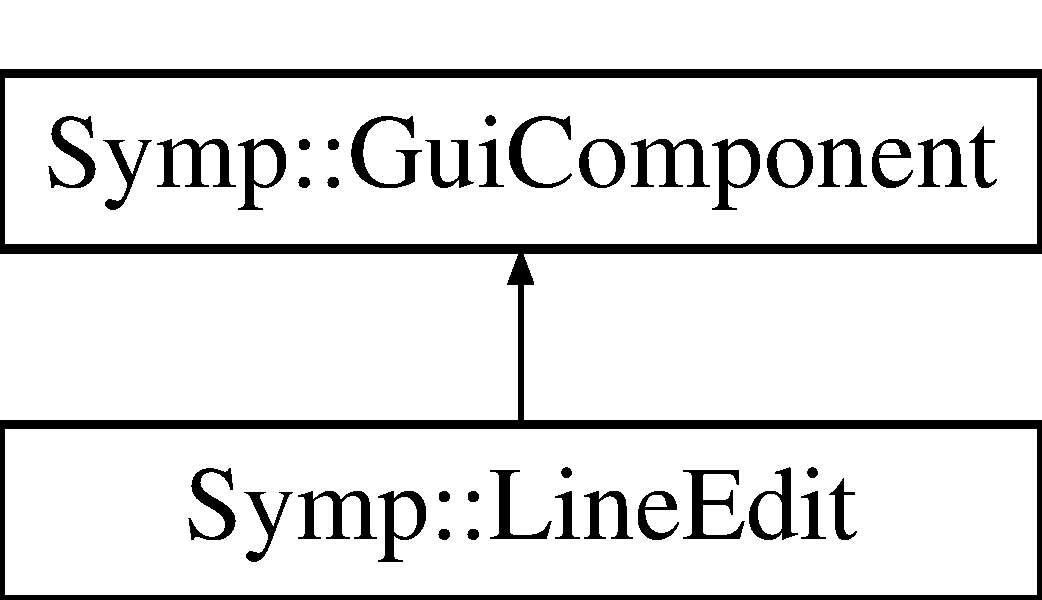
\includegraphics[height=2.000000cm]{class_symp_1_1_line_edit}
\end{center}
\end{figure}
\subsection*{Public Member Functions}
\begin{DoxyCompactItemize}
\item 
\hyperlink{class_symp_1_1_line_edit_aa712aa773e905c7e15f52825006ec65a}{Line\-Edit} (float i\-Pos\-X=0, float i\-Pos\-Y=0, int i\-Width=0, int i\-Height=0)
\begin{DoxyCompactList}\small\item\em \hyperlink{class_symp_1_1_line_edit}{Line\-Edit} constructor Responsible for the initialization of the private attributes of \hyperlink{class_symp_1_1_line_edit_aa712aa773e905c7e15f52825006ec65a}{Line\-Edit} class. \end{DoxyCompactList}\item 
\hyperlink{class_symp_1_1_line_edit_abf14f4506d3824a3facf759862cafd92}{$\sim$\-Line\-Edit} ()
\item 
virtual void \hyperlink{class_symp_1_1_line_edit_a7742de762d2f74e87050ee4086aec9ae}{update} ()
\begin{DoxyCompactList}\small\item\em \hyperlink{class_symp_1_1_line_edit}{Line\-Edit} update fonction Refresh the display of the \hyperlink{class_symp_1_1_line_edit_aa712aa773e905c7e15f52825006ec65a}{Line\-Edit}. \end{DoxyCompactList}\item 
void \hyperlink{class_symp_1_1_line_edit_a7a13f2488719889ef9e905060dfb1cb1}{fill} (\hyperlink{struct_symp_1_1_color}{Symp\-::\-Color} color)
\begin{DoxyCompactList}\small\item\em fill \hyperlink{class_symp_1_1_line_edit}{Line\-Edit}'s background function \end{DoxyCompactList}\item 
void \hyperlink{class_symp_1_1_line_edit_af18768be29c6cd58ebbc9ad37d3aeed7}{trigger\-Focus} ()
\begin{DoxyCompactList}\small\item\em trigger the focus on the \hyperlink{class_symp_1_1_line_edit}{Line\-Edit} \end{DoxyCompactList}\item 
bool \hyperlink{class_symp_1_1_line_edit_a69308c4c24f321dfe5078269aa6e6e47}{has\-Focus} () const 
\item 
\hyperlink{class_symp_1_1_text}{Text} $\ast$ \hyperlink{class_symp_1_1_line_edit_a387dcb8a797ab09456cfbdade58888e0}{get\-Text\-Entity} () const 
\item 
std\-::string \hyperlink{class_symp_1_1_line_edit_a629b33a444f33576093d7fe76bf6fd40}{get\-Text} () const 
\item 
\hyperlink{class_symp_1_1_image}{Image} $\ast$ \hyperlink{class_symp_1_1_line_edit_ab76f79cd92a33d573b88fb1a3d8de905}{get\-Cursor} () const 
\item 
I\-N\-D\-\_\-\-Timer $\ast$ \hyperlink{class_symp_1_1_line_edit_abba8544eeb7029ac07fb46263ccbbf49}{get\-Timer} () const 
\item 
void \hyperlink{class_symp_1_1_line_edit_a3a29ec60c2739eb78f69057fb4caccd3}{set\-Text} (std\-::string text)
\item 
void \hyperlink{class_symp_1_1_line_edit_a277465f59041f7c30ca1688c36db0348}{erase\-Next\-To\-Cursor} ()
\item 
void \hyperlink{class_symp_1_1_line_edit_a2a050cf0268647a6c0e9fff0a4acc1b6}{erase\-Previous\-To\-Cursor} ()
\item 
void \hyperlink{class_symp_1_1_line_edit_a41cceecfc3b0b6b946166b8212b14c8e}{move\-Cursor\-Left} ()
\item 
void \hyperlink{class_symp_1_1_line_edit_a37267fddcdd9505a03a2350ac09f22cb}{move\-Cursor\-Right} ()
\end{DoxyCompactItemize}
\subsection*{Additional Inherited Members}


\subsection{Detailed Description}
the \hyperlink{class_symp_1_1_gui_component_a22124675c2976983ac18374f81cc3fb3}{Gui\-Component} class The \hyperlink{class_symp_1_1_line_edit_aa712aa773e905c7e15f52825006ec65a}{Line\-Edit} class is part of the menu graphical components and can be used only in the menu context. A \hyperlink{class_symp_1_1_line_edit_aa712aa773e905c7e15f52825006ec65a}{Line\-Edit} presents a convenient text input widget that can display the written text, and save it. \begin{DoxyRefDesc}{Todo}
\item[\hyperlink{todo__todo000001}{Todo}]do the class with last version of Indielib font management \end{DoxyRefDesc}
\begin{DoxySeeAlso}{See Also}
\hyperlink{class_symp_1_1_menu_manager}{Menu\-Manager} 

\hyperlink{class_symp_1_1_gui_component}{Gui\-Component} 

\hyperlink{class_symp_1_1_line_edit_aa712aa773e905c7e15f52825006ec65a}{Line\-Edit()} 

\hyperlink{class_symp_1_1_line_edit_abf14f4506d3824a3facf759862cafd92}{$\sim$\-Line\-Edit()} 
\end{DoxySeeAlso}


Definition at line 21 of file Line\-Edit.\-h.



\subsection{Constructor \& Destructor Documentation}
\hypertarget{class_symp_1_1_line_edit_aa712aa773e905c7e15f52825006ec65a}{\index{Symp\-::\-Line\-Edit@{Symp\-::\-Line\-Edit}!Line\-Edit@{Line\-Edit}}
\index{Line\-Edit@{Line\-Edit}!Symp::LineEdit@{Symp\-::\-Line\-Edit}}
\subsubsection[{Line\-Edit}]{\setlength{\rightskip}{0pt plus 5cm}Symp\-::\-Line\-Edit\-::\-Line\-Edit (
\begin{DoxyParamCaption}
\item[{float}]{i\-Pos\-X = {\ttfamily 0}, }
\item[{float}]{i\-Pos\-Y = {\ttfamily 0}, }
\item[{int}]{i\-Width = {\ttfamily 0}, }
\item[{int}]{i\-Height = {\ttfamily 0}}
\end{DoxyParamCaption}
)}}\label{class_symp_1_1_line_edit_aa712aa773e905c7e15f52825006ec65a}


\hyperlink{class_symp_1_1_line_edit}{Line\-Edit} constructor Responsible for the initialization of the private attributes of \hyperlink{class_symp_1_1_line_edit_aa712aa773e905c7e15f52825006ec65a}{Line\-Edit} class. 


\begin{DoxyParams}{Parameters}
{\em i\-Pos\-X} & the x coordinate of the upper-\/left corner of the \hyperlink{class_symp_1_1_line_edit_aa712aa773e905c7e15f52825006ec65a}{Line\-Edit} in pixels \\
\hline
{\em i\-Pos\-Y} & the y coordinate of the upper-\/left corner of the \hyperlink{class_symp_1_1_line_edit_aa712aa773e905c7e15f52825006ec65a}{Line\-Edit} in pixels \\
\hline
{\em i\-Width} & the width of the \hyperlink{class_symp_1_1_line_edit_aa712aa773e905c7e15f52825006ec65a}{Line\-Edit} in pixels \\
\hline
{\em i\-Height} & the height of the \hyperlink{class_symp_1_1_line_edit_aa712aa773e905c7e15f52825006ec65a}{Line\-Edit} in pixels \\
\hline
{\em text} & default none \\
\hline
\end{DoxyParams}
\begin{DoxySeeAlso}{See Also}
\hyperlink{class_symp_1_1_menu_manager}{Menu\-Manager} 

\hyperlink{class_symp_1_1_gui_component}{Gui\-Component} 

\hyperlink{class_symp_1_1_line_edit_abf14f4506d3824a3facf759862cafd92}{$\sim$\-Line\-Edit()} 
\end{DoxySeeAlso}


Definition at line 19 of file Line\-Edit.\-cpp.

\hypertarget{class_symp_1_1_line_edit_abf14f4506d3824a3facf759862cafd92}{\index{Symp\-::\-Line\-Edit@{Symp\-::\-Line\-Edit}!$\sim$\-Line\-Edit@{$\sim$\-Line\-Edit}}
\index{$\sim$\-Line\-Edit@{$\sim$\-Line\-Edit}!Symp::LineEdit@{Symp\-::\-Line\-Edit}}
\subsubsection[{$\sim$\-Line\-Edit}]{\setlength{\rightskip}{0pt plus 5cm}Symp\-::\-Line\-Edit\-::$\sim$\-Line\-Edit (
\begin{DoxyParamCaption}
{}
\end{DoxyParamCaption}
)\hspace{0.3cm}{\ttfamily [inline]}}}\label{class_symp_1_1_line_edit_abf14f4506d3824a3facf759862cafd92}


Definition at line 24 of file Line\-Edit.\-h.



\subsection{Member Function Documentation}
\hypertarget{class_symp_1_1_line_edit_a277465f59041f7c30ca1688c36db0348}{\index{Symp\-::\-Line\-Edit@{Symp\-::\-Line\-Edit}!erase\-Next\-To\-Cursor@{erase\-Next\-To\-Cursor}}
\index{erase\-Next\-To\-Cursor@{erase\-Next\-To\-Cursor}!Symp::LineEdit@{Symp\-::\-Line\-Edit}}
\subsubsection[{erase\-Next\-To\-Cursor}]{\setlength{\rightskip}{0pt plus 5cm}void Symp\-::\-Line\-Edit\-::erase\-Next\-To\-Cursor (
\begin{DoxyParamCaption}
{}
\end{DoxyParamCaption}
)}}\label{class_symp_1_1_line_edit_a277465f59041f7c30ca1688c36db0348}


Definition at line 145 of file Line\-Edit.\-cpp.

\hypertarget{class_symp_1_1_line_edit_a2a050cf0268647a6c0e9fff0a4acc1b6}{\index{Symp\-::\-Line\-Edit@{Symp\-::\-Line\-Edit}!erase\-Previous\-To\-Cursor@{erase\-Previous\-To\-Cursor}}
\index{erase\-Previous\-To\-Cursor@{erase\-Previous\-To\-Cursor}!Symp::LineEdit@{Symp\-::\-Line\-Edit}}
\subsubsection[{erase\-Previous\-To\-Cursor}]{\setlength{\rightskip}{0pt plus 5cm}void Symp\-::\-Line\-Edit\-::erase\-Previous\-To\-Cursor (
\begin{DoxyParamCaption}
{}
\end{DoxyParamCaption}
)}}\label{class_symp_1_1_line_edit_a2a050cf0268647a6c0e9fff0a4acc1b6}


Definition at line 135 of file Line\-Edit.\-cpp.

\hypertarget{class_symp_1_1_line_edit_a7a13f2488719889ef9e905060dfb1cb1}{\index{Symp\-::\-Line\-Edit@{Symp\-::\-Line\-Edit}!fill@{fill}}
\index{fill@{fill}!Symp::LineEdit@{Symp\-::\-Line\-Edit}}
\subsubsection[{fill}]{\setlength{\rightskip}{0pt plus 5cm}void Symp\-::\-Line\-Edit\-::fill (
\begin{DoxyParamCaption}
\item[{{\bf Symp\-::\-Color}}]{color}
\end{DoxyParamCaption}
)}}\label{class_symp_1_1_line_edit_a7a13f2488719889ef9e905060dfb1cb1}


fill \hyperlink{class_symp_1_1_line_edit}{Line\-Edit}'s background function 

\begin{DoxySeeAlso}{See Also}
\hyperlink{class_symp_1_1_line_edit}{Line\-Edit} 

\hyperlink{class_symp_1_1_line_edit_abf14f4506d3824a3facf759862cafd92}{$\sim$\-Line\-Edit()} 

\hyperlink{struct_symp_1_1_color}{Color} 

\hyperlink{class_symp_1_1_gui_component}{Gui\-Component} 
\end{DoxySeeAlso}


Definition at line 86 of file Line\-Edit.\-cpp.

\hypertarget{class_symp_1_1_line_edit_ab76f79cd92a33d573b88fb1a3d8de905}{\index{Symp\-::\-Line\-Edit@{Symp\-::\-Line\-Edit}!get\-Cursor@{get\-Cursor}}
\index{get\-Cursor@{get\-Cursor}!Symp::LineEdit@{Symp\-::\-Line\-Edit}}
\subsubsection[{get\-Cursor}]{\setlength{\rightskip}{0pt plus 5cm}{\bf Image}$\ast$ Symp\-::\-Line\-Edit\-::get\-Cursor (
\begin{DoxyParamCaption}
{}
\end{DoxyParamCaption}
) const\hspace{0.3cm}{\ttfamily [inline]}}}\label{class_symp_1_1_line_edit_ab76f79cd92a33d573b88fb1a3d8de905}


Definition at line 34 of file Line\-Edit.\-h.

\hypertarget{class_symp_1_1_line_edit_a629b33a444f33576093d7fe76bf6fd40}{\index{Symp\-::\-Line\-Edit@{Symp\-::\-Line\-Edit}!get\-Text@{get\-Text}}
\index{get\-Text@{get\-Text}!Symp::LineEdit@{Symp\-::\-Line\-Edit}}
\subsubsection[{get\-Text}]{\setlength{\rightskip}{0pt plus 5cm}std\-::string Symp\-::\-Line\-Edit\-::get\-Text (
\begin{DoxyParamCaption}
{}
\end{DoxyParamCaption}
) const\hspace{0.3cm}{\ttfamily [inline]}}}\label{class_symp_1_1_line_edit_a629b33a444f33576093d7fe76bf6fd40}


Definition at line 33 of file Line\-Edit.\-h.

\hypertarget{class_symp_1_1_line_edit_a387dcb8a797ab09456cfbdade58888e0}{\index{Symp\-::\-Line\-Edit@{Symp\-::\-Line\-Edit}!get\-Text\-Entity@{get\-Text\-Entity}}
\index{get\-Text\-Entity@{get\-Text\-Entity}!Symp::LineEdit@{Symp\-::\-Line\-Edit}}
\subsubsection[{get\-Text\-Entity}]{\setlength{\rightskip}{0pt plus 5cm}{\bf Text}$\ast$ Symp\-::\-Line\-Edit\-::get\-Text\-Entity (
\begin{DoxyParamCaption}
{}
\end{DoxyParamCaption}
) const\hspace{0.3cm}{\ttfamily [inline]}}}\label{class_symp_1_1_line_edit_a387dcb8a797ab09456cfbdade58888e0}


Definition at line 32 of file Line\-Edit.\-h.

\hypertarget{class_symp_1_1_line_edit_abba8544eeb7029ac07fb46263ccbbf49}{\index{Symp\-::\-Line\-Edit@{Symp\-::\-Line\-Edit}!get\-Timer@{get\-Timer}}
\index{get\-Timer@{get\-Timer}!Symp::LineEdit@{Symp\-::\-Line\-Edit}}
\subsubsection[{get\-Timer}]{\setlength{\rightskip}{0pt plus 5cm}I\-N\-D\-\_\-\-Timer$\ast$ Symp\-::\-Line\-Edit\-::get\-Timer (
\begin{DoxyParamCaption}
{}
\end{DoxyParamCaption}
) const\hspace{0.3cm}{\ttfamily [inline]}}}\label{class_symp_1_1_line_edit_abba8544eeb7029ac07fb46263ccbbf49}


Definition at line 35 of file Line\-Edit.\-h.

\hypertarget{class_symp_1_1_line_edit_a69308c4c24f321dfe5078269aa6e6e47}{\index{Symp\-::\-Line\-Edit@{Symp\-::\-Line\-Edit}!has\-Focus@{has\-Focus}}
\index{has\-Focus@{has\-Focus}!Symp::LineEdit@{Symp\-::\-Line\-Edit}}
\subsubsection[{has\-Focus}]{\setlength{\rightskip}{0pt plus 5cm}bool Symp\-::\-Line\-Edit\-::has\-Focus (
\begin{DoxyParamCaption}
{}
\end{DoxyParamCaption}
) const\hspace{0.3cm}{\ttfamily [inline]}}}\label{class_symp_1_1_line_edit_a69308c4c24f321dfe5078269aa6e6e47}


Definition at line 31 of file Line\-Edit.\-h.

\hypertarget{class_symp_1_1_line_edit_a41cceecfc3b0b6b946166b8212b14c8e}{\index{Symp\-::\-Line\-Edit@{Symp\-::\-Line\-Edit}!move\-Cursor\-Left@{move\-Cursor\-Left}}
\index{move\-Cursor\-Left@{move\-Cursor\-Left}!Symp::LineEdit@{Symp\-::\-Line\-Edit}}
\subsubsection[{move\-Cursor\-Left}]{\setlength{\rightskip}{0pt plus 5cm}void Symp\-::\-Line\-Edit\-::move\-Cursor\-Left (
\begin{DoxyParamCaption}
{}
\end{DoxyParamCaption}
)}}\label{class_symp_1_1_line_edit_a41cceecfc3b0b6b946166b8212b14c8e}


Definition at line 121 of file Line\-Edit.\-cpp.

\hypertarget{class_symp_1_1_line_edit_a37267fddcdd9505a03a2350ac09f22cb}{\index{Symp\-::\-Line\-Edit@{Symp\-::\-Line\-Edit}!move\-Cursor\-Right@{move\-Cursor\-Right}}
\index{move\-Cursor\-Right@{move\-Cursor\-Right}!Symp::LineEdit@{Symp\-::\-Line\-Edit}}
\subsubsection[{move\-Cursor\-Right}]{\setlength{\rightskip}{0pt plus 5cm}void Symp\-::\-Line\-Edit\-::move\-Cursor\-Right (
\begin{DoxyParamCaption}
{}
\end{DoxyParamCaption}
)}}\label{class_symp_1_1_line_edit_a37267fddcdd9505a03a2350ac09f22cb}


Definition at line 128 of file Line\-Edit.\-cpp.

\hypertarget{class_symp_1_1_line_edit_a3a29ec60c2739eb78f69057fb4caccd3}{\index{Symp\-::\-Line\-Edit@{Symp\-::\-Line\-Edit}!set\-Text@{set\-Text}}
\index{set\-Text@{set\-Text}!Symp::LineEdit@{Symp\-::\-Line\-Edit}}
\subsubsection[{set\-Text}]{\setlength{\rightskip}{0pt plus 5cm}void Symp\-::\-Line\-Edit\-::set\-Text (
\begin{DoxyParamCaption}
\item[{std\-::string}]{text}
\end{DoxyParamCaption}
)}}\label{class_symp_1_1_line_edit_a3a29ec60c2739eb78f69057fb4caccd3}


Definition at line 115 of file Line\-Edit.\-cpp.

\hypertarget{class_symp_1_1_line_edit_af18768be29c6cd58ebbc9ad37d3aeed7}{\index{Symp\-::\-Line\-Edit@{Symp\-::\-Line\-Edit}!trigger\-Focus@{trigger\-Focus}}
\index{trigger\-Focus@{trigger\-Focus}!Symp::LineEdit@{Symp\-::\-Line\-Edit}}
\subsubsection[{trigger\-Focus}]{\setlength{\rightskip}{0pt plus 5cm}void Symp\-::\-Line\-Edit\-::trigger\-Focus (
\begin{DoxyParamCaption}
{}
\end{DoxyParamCaption}
)}}\label{class_symp_1_1_line_edit_af18768be29c6cd58ebbc9ad37d3aeed7}


trigger the focus on the \hyperlink{class_symp_1_1_line_edit}{Line\-Edit} 

\begin{DoxySeeAlso}{See Also}
\hyperlink{class_symp_1_1_line_edit}{Line\-Edit} 

\hyperlink{class_symp_1_1_line_edit_abf14f4506d3824a3facf759862cafd92}{$\sim$\-Line\-Edit()} 

\hyperlink{class_symp_1_1_gui_component}{Gui\-Component} 
\end{DoxySeeAlso}


Definition at line 97 of file Line\-Edit.\-cpp.

\hypertarget{class_symp_1_1_line_edit_a7742de762d2f74e87050ee4086aec9ae}{\index{Symp\-::\-Line\-Edit@{Symp\-::\-Line\-Edit}!update@{update}}
\index{update@{update}!Symp::LineEdit@{Symp\-::\-Line\-Edit}}
\subsubsection[{update}]{\setlength{\rightskip}{0pt plus 5cm}void Symp\-::\-Line\-Edit\-::update (
\begin{DoxyParamCaption}
{}
\end{DoxyParamCaption}
)\hspace{0.3cm}{\ttfamily [virtual]}}}\label{class_symp_1_1_line_edit_a7742de762d2f74e87050ee4086aec9ae}


\hyperlink{class_symp_1_1_line_edit}{Line\-Edit} update fonction Refresh the display of the \hyperlink{class_symp_1_1_line_edit_aa712aa773e905c7e15f52825006ec65a}{Line\-Edit}. 

\begin{DoxySeeAlso}{See Also}
\hyperlink{class_symp_1_1_line_edit}{Line\-Edit} 

\hyperlink{class_symp_1_1_line_edit_abf14f4506d3824a3facf759862cafd92}{$\sim$\-Line\-Edit()} 

\hyperlink{class_symp_1_1_gui_component}{Gui\-Component} 
\end{DoxySeeAlso}


Implements \hyperlink{class_symp_1_1_gui_component_add73e07ea0a3c9c1c90640e783a3b5de}{Symp\-::\-Gui\-Component}.



Definition at line 57 of file Line\-Edit.\-cpp.



The documentation for this class was generated from the following files\-:\begin{DoxyCompactItemize}
\item 
/home/cecilia/\-Documents/\-Symptogen/src/menu/\hyperlink{_line_edit_8h}{Line\-Edit.\-h}\item 
/home/cecilia/\-Documents/\-Symptogen/src/menu/\hyperlink{_line_edit_8cpp}{Line\-Edit.\-cpp}\end{DoxyCompactItemize}

\hypertarget{class_symp_1_1_manage_games_menu}{\section{Symp\-:\-:Manage\-Games\-Menu Class Reference}
\label{class_symp_1_1_manage_games_menu}\index{Symp\-::\-Manage\-Games\-Menu@{Symp\-::\-Manage\-Games\-Menu}}
}


{\ttfamily \#include $<$Manage\-Games\-Menu.\-h$>$}

Inheritance diagram for Symp\-:\-:Manage\-Games\-Menu\-:\begin{figure}[H]
\begin{center}
\leavevmode
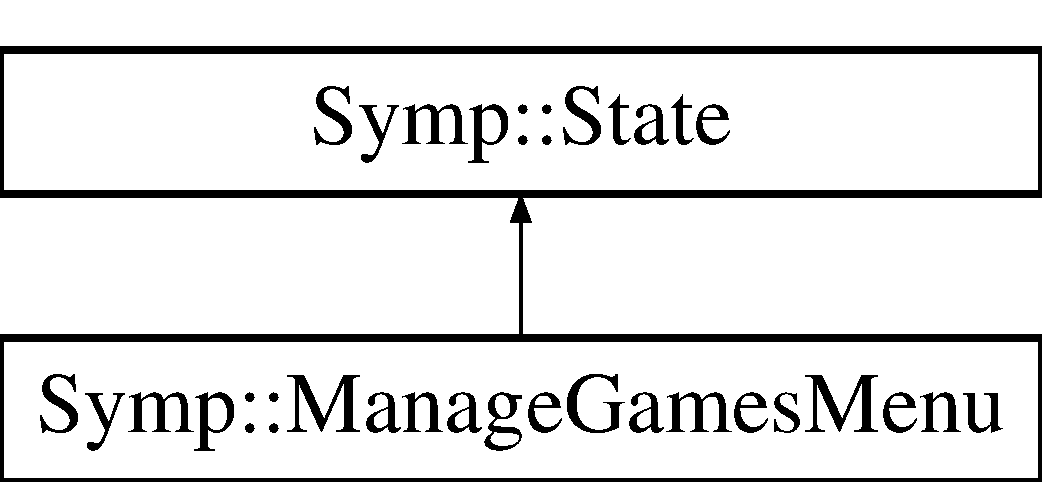
\includegraphics[height=2.000000cm]{class_symp_1_1_manage_games_menu}
\end{center}
\end{figure}
\subsection*{Public Member Functions}
\begin{DoxyCompactItemize}
\item 
\hyperlink{class_symp_1_1_manage_games_menu_a67b463e96bf9c5716f349573860ae0cb}{Manage\-Games\-Menu} ()
\begin{DoxyCompactList}\small\item\em \hyperlink{class_symp_1_1_manage_games_menu}{Manage\-Games\-Menu} constructor Responsible for the initialization of the private attributes of the \#\-Manage\-Games\-Menu\-Menu class. This function is not responsible for drawing the graphical elements that compose the menu, the \hyperlink{class_symp_1_1_manage_games_menu_a2cac1836c3c7272633a99beb0287f9b1}{init()} function is. \end{DoxyCompactList}\item 
\hyperlink{class_symp_1_1_manage_games_menu_aa12c9e144cc1421ad6fefa7c4c140530}{$\sim$\-Manage\-Games\-Menu} ()
\item 
virtual void \hyperlink{class_symp_1_1_manage_games_menu_a2cac1836c3c7272633a99beb0287f9b1}{init} ()
\begin{DoxyCompactList}\small\item\em \hyperlink{class_symp_1_1_manage_games_menu}{Manage\-Games\-Menu} elements initialization The elements that compose the menu are created in this function. \end{DoxyCompactList}\item 
virtual void \hyperlink{class_symp_1_1_manage_games_menu_acbca4c010ddb4a39fcdc1b0e3716bb03}{handle\-Mouse\-Clic} (int mouse\-X, int mouse\-Y)
\begin{DoxyCompactList}\small\item\em Handle mouse clic events. \end{DoxyCompactList}\item 
virtual void \hyperlink{class_symp_1_1_manage_games_menu_ab330c9d8b0103d7232dc698e01d8e820}{key\-Down\-Pressed} ()
\begin{DoxyCompactList}\small\item\em Handle key down event. \end{DoxyCompactList}\item 
virtual void \hyperlink{class_symp_1_1_manage_games_menu_a31141c164d9d36c51eb1a0b5803f0974}{key\-Up\-Pressed} ()
\begin{DoxyCompactList}\small\item\em Handle key up event. \end{DoxyCompactList}\item 
std\-::string \hyperlink{class_symp_1_1_manage_games_menu_a1d36113bc83871b8cb028d1691ac3d58}{get\-Level\-Name} (int level)
\item 
\hyperlink{class_symp_1_1_layout}{Layout} $\ast$ \hyperlink{class_symp_1_1_manage_games_menu_ae468d3d6d1972468065e100003ecfec9}{create\-Player\-Panel} (\hyperlink{class_symp_1_1_player}{Player} $\ast$p\-Player, int i\-Pos\-X, int i\-Pos\-Y, int i\-Width, int i\-Height, \hyperlink{struct_symp_1_1_color}{Color} border\-Color, \hyperlink{struct_symp_1_1_color}{Color} background\-Color)
\begin{DoxyCompactList}\small\item\em Create a panel with the \#\-Player data The elements that compose the \#\-Player panel are created in this function. This panel is composed by a \#\-Layout that group elements but that do not manage their position and shape, and a \#\-Button that can receive events. The panel can be customized with two colors \-: one for the border of the \#\-Layout component, one for the background of the \#\-Button component. \end{DoxyCompactList}\end{DoxyCompactItemize}


\subsection{Detailed Description}
the \hyperlink{class_symp_1_1_state_ad44d90b6e1b68eb021ceaa0cb98141a4}{State} interface for implementing the \hyperlink{class_symp_1_1_state}{State} Machine Pattern This Menu show the list of the players currently registrated into the application. The last \#\-Player is shown above the other. The click on a \#\-Player panel will bring the user to the specific \#\-Player menu \#\-Choose\-Your\-Level\-Menu. The user can create a new \#\-Player from this menu, or go back to the main menu. \begin{DoxySeeAlso}{See Also}
\hyperlink{class_symp_1_1_state}{State} 

\hyperlink{class_symp_1_1_game_manager}{Game\-Manager} 

\hyperlink{class_symp_1_1_choose_your_level_menu}{Choose\-Your\-Level\-Menu} 

\hyperlink{class_symp_1_1_welcome_last_player_menu}{Welcome\-Last\-Player\-Menu} 

\hyperlink{class_symp_1_1_menu_manager}{Menu\-Manager} 
\end{DoxySeeAlso}


Definition at line 21 of file Manage\-Games\-Menu.\-h.



\subsection{Constructor \& Destructor Documentation}
\hypertarget{class_symp_1_1_manage_games_menu_a67b463e96bf9c5716f349573860ae0cb}{\index{Symp\-::\-Manage\-Games\-Menu@{Symp\-::\-Manage\-Games\-Menu}!Manage\-Games\-Menu@{Manage\-Games\-Menu}}
\index{Manage\-Games\-Menu@{Manage\-Games\-Menu}!Symp::ManageGamesMenu@{Symp\-::\-Manage\-Games\-Menu}}
\subsubsection[{Manage\-Games\-Menu}]{\setlength{\rightskip}{0pt plus 5cm}Symp\-::\-Manage\-Games\-Menu\-::\-Manage\-Games\-Menu (
\begin{DoxyParamCaption}
{}
\end{DoxyParamCaption}
)}}\label{class_symp_1_1_manage_games_menu_a67b463e96bf9c5716f349573860ae0cb}


\hyperlink{class_symp_1_1_manage_games_menu}{Manage\-Games\-Menu} constructor Responsible for the initialization of the private attributes of the \#\-Manage\-Games\-Menu\-Menu class. This function is not responsible for drawing the graphical elements that compose the menu, the \hyperlink{class_symp_1_1_manage_games_menu_a2cac1836c3c7272633a99beb0287f9b1}{init()} function is. 

\begin{DoxySeeAlso}{See Also}
\hyperlink{class_symp_1_1_player}{Player} 

\hyperlink{class_symp_1_1_menu_manager}{Menu\-Manager} 

\hyperlink{class_symp_1_1_state}{State} 

\hyperlink{class_symp_1_1_manage_games_menu_a2cac1836c3c7272633a99beb0287f9b1}{init()} 

\hyperlink{class_symp_1_1_manage_games_menu_aa12c9e144cc1421ad6fefa7c4c140530}{$\sim$\-Manage\-Games\-Menu()} 
\end{DoxySeeAlso}


Definition at line 23 of file Manage\-Games\-Menu.\-cpp.

\hypertarget{class_symp_1_1_manage_games_menu_aa12c9e144cc1421ad6fefa7c4c140530}{\index{Symp\-::\-Manage\-Games\-Menu@{Symp\-::\-Manage\-Games\-Menu}!$\sim$\-Manage\-Games\-Menu@{$\sim$\-Manage\-Games\-Menu}}
\index{$\sim$\-Manage\-Games\-Menu@{$\sim$\-Manage\-Games\-Menu}!Symp::ManageGamesMenu@{Symp\-::\-Manage\-Games\-Menu}}
\subsubsection[{$\sim$\-Manage\-Games\-Menu}]{\setlength{\rightskip}{0pt plus 5cm}Symp\-::\-Manage\-Games\-Menu\-::$\sim$\-Manage\-Games\-Menu (
\begin{DoxyParamCaption}
{}
\end{DoxyParamCaption}
)\hspace{0.3cm}{\ttfamily [inline]}}}\label{class_symp_1_1_manage_games_menu_aa12c9e144cc1421ad6fefa7c4c140530}


Definition at line 24 of file Manage\-Games\-Menu.\-h.



\subsection{Member Function Documentation}
\hypertarget{class_symp_1_1_manage_games_menu_ae468d3d6d1972468065e100003ecfec9}{\index{Symp\-::\-Manage\-Games\-Menu@{Symp\-::\-Manage\-Games\-Menu}!create\-Player\-Panel@{create\-Player\-Panel}}
\index{create\-Player\-Panel@{create\-Player\-Panel}!Symp::ManageGamesMenu@{Symp\-::\-Manage\-Games\-Menu}}
\subsubsection[{create\-Player\-Panel}]{\setlength{\rightskip}{0pt plus 5cm}{\bf Layout} $\ast$ Symp\-::\-Manage\-Games\-Menu\-::create\-Player\-Panel (
\begin{DoxyParamCaption}
\item[{{\bf Player} $\ast$}]{p\-Player, }
\item[{int}]{i\-Pos\-X, }
\item[{int}]{i\-Pos\-Y, }
\item[{int}]{i\-Width, }
\item[{int}]{i\-Height, }
\item[{{\bf Color}}]{border\-Color, }
\item[{{\bf Color}}]{background\-Color}
\end{DoxyParamCaption}
)}}\label{class_symp_1_1_manage_games_menu_ae468d3d6d1972468065e100003ecfec9}


Create a panel with the \#\-Player data The elements that compose the \#\-Player panel are created in this function. This panel is composed by a \#\-Layout that group elements but that do not manage their position and shape, and a \#\-Button that can receive events. The panel can be customized with two colors \-: one for the border of the \#\-Layout component, one for the background of the \#\-Button component. 


\begin{DoxyParams}{Parameters}
{\em p\-Player} & the reference to the \#\-Player this panel is made for \\
\hline
{\em i\-Pos\-X} & the x coordinate of the upper-\/left corner of the panel in pixels \\
\hline
{\em i\-Pos\-Y} & the y coordinate of the upper-\/left corner of the panel in pixels \\
\hline
{\em i\-Width} & the width of the panel in pixels \\
\hline
{\em i\-Height} & the height of the panel in pixels \\
\hline
{\em border\-Color} & the color of the border of the panel \\
\hline
{\em backgound\-Color} & the color of the background of the panel \\
\hline
\end{DoxyParams}
\begin{DoxyReturn}{Returns}
p\-Layout the reference to the \#\-Layout that contain the \#\-Player graphcal data 
\end{DoxyReturn}
\begin{DoxySeeAlso}{See Also}
\hyperlink{class_symp_1_1_player}{Player} 

\hyperlink{class_symp_1_1_menu_manager}{Menu\-Manager} 

\hyperlink{class_symp_1_1_state}{State} 

\hyperlink{class_symp_1_1_manage_games_menu_a2cac1836c3c7272633a99beb0287f9b1}{init()} 
\end{DoxySeeAlso}


Definition at line 106 of file Manage\-Games\-Menu.\-cpp.

\hypertarget{class_symp_1_1_manage_games_menu_a1d36113bc83871b8cb028d1691ac3d58}{\index{Symp\-::\-Manage\-Games\-Menu@{Symp\-::\-Manage\-Games\-Menu}!get\-Level\-Name@{get\-Level\-Name}}
\index{get\-Level\-Name@{get\-Level\-Name}!Symp::ManageGamesMenu@{Symp\-::\-Manage\-Games\-Menu}}
\subsubsection[{get\-Level\-Name}]{\setlength{\rightskip}{0pt plus 5cm}std\-::string Symp\-::\-Manage\-Games\-Menu\-::get\-Level\-Name (
\begin{DoxyParamCaption}
\item[{int}]{level}
\end{DoxyParamCaption}
)}}\label{class_symp_1_1_manage_games_menu_a1d36113bc83871b8cb028d1691ac3d58}


Definition at line 211 of file Manage\-Games\-Menu.\-cpp.

\hypertarget{class_symp_1_1_manage_games_menu_acbca4c010ddb4a39fcdc1b0e3716bb03}{\index{Symp\-::\-Manage\-Games\-Menu@{Symp\-::\-Manage\-Games\-Menu}!handle\-Mouse\-Clic@{handle\-Mouse\-Clic}}
\index{handle\-Mouse\-Clic@{handle\-Mouse\-Clic}!Symp::ManageGamesMenu@{Symp\-::\-Manage\-Games\-Menu}}
\subsubsection[{handle\-Mouse\-Clic}]{\setlength{\rightskip}{0pt plus 5cm}void Symp\-::\-Manage\-Games\-Menu\-::handle\-Mouse\-Clic (
\begin{DoxyParamCaption}
\item[{int}]{mouse\-X, }
\item[{int}]{mouse\-Y}
\end{DoxyParamCaption}
)\hspace{0.3cm}{\ttfamily [virtual]}}}\label{class_symp_1_1_manage_games_menu_acbca4c010ddb4a39fcdc1b0e3716bb03}


Handle mouse clic events. 


\begin{DoxyParams}{Parameters}
{\em mouse\-X} & the x coordinate of the mouse position \\
\hline
{\em mouse\-Y} & the y coordinate of the mouse position \\
\hline
\end{DoxyParams}
\begin{DoxySeeAlso}{See Also}
\hyperlink{class_symp_1_1_menu_manager}{Menu\-Manager} 

\hyperlink{class_symp_1_1_state}{State} 

\hyperlink{class_symp_1_1_input_manager}{Input\-Manager} 

\hyperlink{class_symp_1_1_manage_games_menu_a2cac1836c3c7272633a99beb0287f9b1}{init()} 
\end{DoxySeeAlso}


Implements \hyperlink{class_symp_1_1_state_a23e468a10d9be4c79d17e22d1d5ef478}{Symp\-::\-State}.



Definition at line 178 of file Manage\-Games\-Menu.\-cpp.

\hypertarget{class_symp_1_1_manage_games_menu_a2cac1836c3c7272633a99beb0287f9b1}{\index{Symp\-::\-Manage\-Games\-Menu@{Symp\-::\-Manage\-Games\-Menu}!init@{init}}
\index{init@{init}!Symp::ManageGamesMenu@{Symp\-::\-Manage\-Games\-Menu}}
\subsubsection[{init}]{\setlength{\rightskip}{0pt plus 5cm}void Symp\-::\-Manage\-Games\-Menu\-::init (
\begin{DoxyParamCaption}
{}
\end{DoxyParamCaption}
)\hspace{0.3cm}{\ttfamily [virtual]}}}\label{class_symp_1_1_manage_games_menu_a2cac1836c3c7272633a99beb0287f9b1}


\hyperlink{class_symp_1_1_manage_games_menu}{Manage\-Games\-Menu} elements initialization The elements that compose the menu are created in this function. 

\begin{DoxySeeAlso}{See Also}
\hyperlink{class_symp_1_1_player}{Player} 

\hyperlink{class_symp_1_1_menu_manager}{Menu\-Manager} 

\hyperlink{class_symp_1_1_state}{State} 

end() 
\end{DoxySeeAlso}


Implements \hyperlink{class_symp_1_1_state_a2c1c597b1235128a356c7529c42fdec3}{Symp\-::\-State}.



Definition at line 36 of file Manage\-Games\-Menu.\-cpp.

\hypertarget{class_symp_1_1_manage_games_menu_ab330c9d8b0103d7232dc698e01d8e820}{\index{Symp\-::\-Manage\-Games\-Menu@{Symp\-::\-Manage\-Games\-Menu}!key\-Down\-Pressed@{key\-Down\-Pressed}}
\index{key\-Down\-Pressed@{key\-Down\-Pressed}!Symp::ManageGamesMenu@{Symp\-::\-Manage\-Games\-Menu}}
\subsubsection[{key\-Down\-Pressed}]{\setlength{\rightskip}{0pt plus 5cm}void Symp\-::\-Manage\-Games\-Menu\-::key\-Down\-Pressed (
\begin{DoxyParamCaption}
{}
\end{DoxyParamCaption}
)\hspace{0.3cm}{\ttfamily [virtual]}}}\label{class_symp_1_1_manage_games_menu_ab330c9d8b0103d7232dc698e01d8e820}


Handle key down event. 

\begin{DoxySeeAlso}{See Also}
\hyperlink{class_symp_1_1_menu_manager}{Menu\-Manager} 

\hyperlink{class_symp_1_1_state}{State} 

\hyperlink{class_symp_1_1_input_manager}{Input\-Manager} 

\hyperlink{class_symp_1_1_manage_games_menu_a2cac1836c3c7272633a99beb0287f9b1}{init()} 
\end{DoxySeeAlso}


Implements \hyperlink{class_symp_1_1_state_ac9ff920d185cdc17c9bc3ac63b40c62d}{Symp\-::\-State}.



Definition at line 238 of file Manage\-Games\-Menu.\-cpp.

\hypertarget{class_symp_1_1_manage_games_menu_a31141c164d9d36c51eb1a0b5803f0974}{\index{Symp\-::\-Manage\-Games\-Menu@{Symp\-::\-Manage\-Games\-Menu}!key\-Up\-Pressed@{key\-Up\-Pressed}}
\index{key\-Up\-Pressed@{key\-Up\-Pressed}!Symp::ManageGamesMenu@{Symp\-::\-Manage\-Games\-Menu}}
\subsubsection[{key\-Up\-Pressed}]{\setlength{\rightskip}{0pt plus 5cm}void Symp\-::\-Manage\-Games\-Menu\-::key\-Up\-Pressed (
\begin{DoxyParamCaption}
{}
\end{DoxyParamCaption}
)\hspace{0.3cm}{\ttfamily [virtual]}}}\label{class_symp_1_1_manage_games_menu_a31141c164d9d36c51eb1a0b5803f0974}


Handle key up event. 

\begin{DoxySeeAlso}{See Also}
\hyperlink{class_symp_1_1_menu_manager}{Menu\-Manager} 

\hyperlink{class_symp_1_1_state}{State} 

\hyperlink{class_symp_1_1_input_manager}{Input\-Manager} 

\hyperlink{class_symp_1_1_manage_games_menu_a2cac1836c3c7272633a99beb0287f9b1}{init()} 
\end{DoxySeeAlso}


Implements \hyperlink{class_symp_1_1_state_a67d0fc2a02808bbcfdb06935c3be404f}{Symp\-::\-State}.



Definition at line 248 of file Manage\-Games\-Menu.\-cpp.



The documentation for this class was generated from the following files\-:\begin{DoxyCompactItemize}
\item 
/home/cecilia/\-Documents/\-Symptogen/src/menu/\hyperlink{_manage_games_menu_8h}{Manage\-Games\-Menu.\-h}\item 
/home/cecilia/\-Documents/\-Symptogen/src/menu/\hyperlink{_manage_games_menu_8cpp}{Manage\-Games\-Menu.\-cpp}\end{DoxyCompactItemize}

\hypertarget{class_symp_1_1_menu_manager}{\section{Symp\-:\-:Menu\-Manager Class Reference}
\label{class_symp_1_1_menu_manager}\index{Symp\-::\-Menu\-Manager@{Symp\-::\-Menu\-Manager}}
}


{\ttfamily \#include $<$Menu\-Manager.\-h$>$}

Inheritance diagram for Symp\-:\-:Menu\-Manager\-:\begin{figure}[H]
\begin{center}
\leavevmode
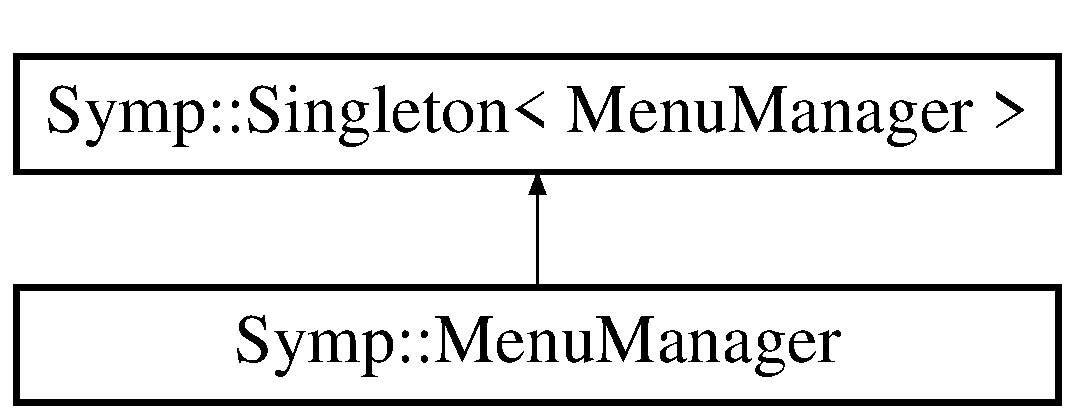
\includegraphics[height=2.000000cm]{class_symp_1_1_menu_manager}
\end{center}
\end{figure}
\subsection*{Public Member Functions}
\begin{DoxyCompactItemize}
\item 
void \hyperlink{class_symp_1_1_menu_manager_aab6441e17669df816e59689cc8abf9d9}{init} (\hyperlink{class_symp_1_1_render}{Render} $\ast$p\-Render, std\-::pair$<$ \hyperlink{class_symp_1_1_player}{Player} $\ast$, std\-::vector$<$ \hyperlink{class_symp_1_1_player}{Player} $\ast$ $>$$>$ player\-Data)
\item 
bool \hyperlink{class_symp_1_1_menu_manager_a76a689b279833c2b6f8605fc091d6889}{add\-Gui\-Component} (\hyperlink{class_symp_1_1_gui_component}{Gui\-Component} $\ast$gui\-Component, int layer)
\begin{DoxyCompactList}\small\item\em Add a component to the Indielib and \hyperlink{class_symp_1_1_menu_manager}{Menu\-Manager} containers When a menu needs to render a component, the component is added by this function in both containers of the \hyperlink{class_symp_1_1_menu_manager}{Menu\-Manager} and the Indielib library \-: the first to store historic and the second to pass to the renderer. \end{DoxyCompactList}\item 
void \hyperlink{class_symp_1_1_menu_manager_ab5eb90e375b4832e284804d0e985afe9}{add\-Gui\-Layout} (\hyperlink{class_symp_1_1_layout}{Layout} $\ast$layout, int layer)
\begin{DoxyCompactList}\small\item\em Add a layout and its components to the Indielib and \hyperlink{class_symp_1_1_menu_manager}{Menu\-Manager} containers A \hyperlink{class_symp_1_1_layout}{Layout} contains multiple Gui\-Components, and all need to be added to the Indie\-Lib and \hyperlink{class_symp_1_1_menu_manager}{Menu\-Manager} containers. \end{DoxyCompactList}\item 
void \hyperlink{class_symp_1_1_menu_manager_ad72c273480039d17ebda3480311d4508}{handle\-Mouse\-Clic} (int mouse\-X, int mouse\-Y)
\begin{DoxyCompactList}\small\item\em Handle the mouse clic event The \hyperlink{class_symp_1_1_game_manager}{Game\-Manager} pass the mouve clic to the \hyperlink{class_symp_1_1_menu_manager}{Menu\-Manager} if the menus are currently displayed. The \hyperlink{class_symp_1_1_menu_manager}{Menu\-Manager} passes the event to its current state that manage the response to the event. \end{DoxyCompactList}\item 
void \hyperlink{class_symp_1_1_menu_manager_a227969f9ba1824e4d490d6ff8c2293f0}{handle\-Key\-Pressed} (std\-::string key)
\begin{DoxyCompactList}\small\item\em Handle the key press event The \hyperlink{class_symp_1_1_game_manager}{Game\-Manager} pass the key press to the \hyperlink{class_symp_1_1_menu_manager}{Menu\-Manager} if the menus are currently displayed. The \hyperlink{class_symp_1_1_menu_manager}{Menu\-Manager} passes the event to its current state that manage the response to the event. \end{DoxyCompactList}\item 
void \hyperlink{class_symp_1_1_menu_manager_adfcb55f36a13d91538c789fdc4f5dd14}{handle\-Mouse\-Hover} (int mouse\-X, int mouse\-Y)
\begin{DoxyCompactList}\small\item\em Handle the mouse hover event The \hyperlink{class_symp_1_1_game_manager}{Game\-Manager} pass the mouve hover to the \hyperlink{class_symp_1_1_menu_manager}{Menu\-Manager} if the menus are currently displayed. The \hyperlink{class_symp_1_1_menu_manager}{Menu\-Manager} owns the Gui\-Components currently displayed by its actual state, and can tell them if there are hovered or not. That can make the Gui\-Components update their appearence. This event is the only one that is not passed to the current state. \end{DoxyCompactList}\item 
void \hyperlink{class_symp_1_1_menu_manager_a83ab1aa4099241f934f55968418487a7}{render\-Entities} ()
\begin{DoxyCompactList}\small\item\em Command to the Indielib library which layers of components are displayed When a component is added to the Indielib I\-N\-D\-\_\-\-Entity2d\-Manager, it is placed in a layer. A layer can group component and can be displayed or not. \end{DoxyCompactList}\item 
void \hyperlink{class_symp_1_1_menu_manager_ac452e8136cb2369b0e2803452f64cc6b}{clear} ()
\begin{DoxyCompactList}\small\item\em Function that erase the Indielib components. When the game world and components needs to be displayed, the Indielib menu components have to be removed in order not to be displayed anymore on the screen. \end{DoxyCompactList}\item 
void \hyperlink{class_symp_1_1_menu_manager_ad91c22c5324edaf941b4a8d4c13bc3f6}{go\-Back} ()
\begin{DoxyCompactList}\small\item\em Retrieve the previous state the \hyperlink{class_symp_1_1_menu_manager}{Menu\-Manager} was in As the \hyperlink{class_symp_1_1_menu_manager}{Menu\-Manager} is part of a state machine pattern, a menu is a state and displaying a new menu means changing current state. The history of menus is stored and can be traced back, without changing the history itself. The opposite of the go\-Back method is the set\-State method that update the history. \end{DoxyCompactList}\item 
void \hyperlink{class_symp_1_1_menu_manager_acc745b44f27394f6760bfb09884ea289}{erase\-Player\-Data} (\hyperlink{class_symp_1_1_player}{Player} $\ast$player)
\item 
void \hyperlink{class_symp_1_1_menu_manager_a1ffcae1937e8eb6d4cd2014c91e05988}{reload\-Data} (std\-::pair$<$ \hyperlink{class_symp_1_1_player}{Player} $\ast$, std\-::vector$<$ \hyperlink{class_symp_1_1_player}{Player} $\ast$ $>$$>$ player\-Data)
\item 
void \hyperlink{class_symp_1_1_menu_manager_a2c082ed56b628e636b7a39ecb244ce23}{set\-Level\-To\-Load} (std\-::string s\-Path)
\item 
void \hyperlink{class_symp_1_1_menu_manager_a6d8d4373c4a0de222eb11c3aa4040684}{set\-State} (\hyperlink{class_symp_1_1_state}{State} $\ast$p\-State)
\begin{DoxyCompactList}\small\item\em Change the current state of the \hyperlink{class_symp_1_1_menu_manager}{Menu\-Manager} As the \hyperlink{class_symp_1_1_menu_manager}{Menu\-Manager} is part of a state machine pattern, a menu is a state and displaying a new menu means changing current state. The old state needs to be removed. When the new state is settled as the current state, the state is initialized and its components added to the \hyperlink{class_symp_1_1_menu_manager}{Menu\-Manager} and Indielib containers. The history can be traced back with the go\-Back method. \end{DoxyCompactList}\item 
void \hyperlink{class_symp_1_1_menu_manager_a548086a6bc43e59eb9fb51f7b030e009}{set\-Level\-Choosen} (bool b\-Value)
\item 
void \hyperlink{class_symp_1_1_menu_manager_a588955c6be0b4e0c02024a3f99bf489c}{set\-Is\-Displaying\-Pause\-State} (bool b\-Value)
\item 
void \hyperlink{class_symp_1_1_menu_manager_af81f00489117749ab084064b6a386166}{set\-Is\-Going\-Back\-To\-Menu} (bool value)
\item 
void \hyperlink{class_symp_1_1_menu_manager_a6bac0d174a5b3af95df602c7d5f36b02}{set\-Is\-About\-To\-Quit} (bool value)
\item 
void \hyperlink{class_symp_1_1_menu_manager_ae02940a8786e8959fe45a8b48bb3dfb8}{set\-Has\-Line\-Edit\-Focus} (bool value)
\item 
void \hyperlink{class_symp_1_1_menu_manager_a31bad57ff718192aab5aa951d809ce8f}{set\-Last\-Player} (\hyperlink{class_symp_1_1_player}{Player} $\ast$player)
\item 
void \hyperlink{class_symp_1_1_menu_manager_aa08c2c34c8dc95199f5250e87aeaf13d}{set\-Players} (std\-::vector$<$ \hyperlink{class_symp_1_1_player}{Player} $\ast$ $>$ players)
\item 
void \hyperlink{class_symp_1_1_menu_manager_a269895498ed2ed92ead3b9e628e8ce98}{set\-Has\-Player\-Data\-Changed} (bool value)
\item 
void \hyperlink{class_symp_1_1_menu_manager_aa686e7c72abd63486a6ce3d5a236fc34}{set\-Player\-Index} (int index)
\item 
\hyperlink{class_symp_1_1_player}{Player} $\ast$ \hyperlink{class_symp_1_1_menu_manager_a086e53a1c9799b72a0fc8606549a4824}{get\-Last\-Player} () const 
\item 
std\-::vector$<$ \hyperlink{class_symp_1_1_player}{Player} $\ast$ $>$ \hyperlink{class_symp_1_1_menu_manager_a464da67bcfec32b635d160a29520522b}{get\-Players} () const 
\item 
std\-::string \hyperlink{class_symp_1_1_menu_manager_a51fa8c805528a8a4bd2e834df3f99ad3}{get\-Level\-To\-Load} () const 
\item 
I\-N\-D\-\_\-\-Entity2d\-Manager $\ast$ \hyperlink{class_symp_1_1_menu_manager_a8fe8763dd656f9a149d009883437fa90}{get\-I\-N\-D\-\_\-\-Entity2d\-Manager} () const 
\item 
\hyperlink{class_symp_1_1_state}{State} $\ast$ \hyperlink{class_symp_1_1_menu_manager_a3c0bbc01aff2632a73bfb4183e485b24}{get\-Current\-State} () const 
\item 
std\-::vector$<$ \hyperlink{class_symp_1_1_gui_component}{Gui\-Component} $\ast$ $>$ \hyperlink{class_symp_1_1_menu_manager_a61f93678d0dbaa5408d3904912a59b7f}{get\-Gui\-Component\-Array} () const 
\item 
int \hyperlink{class_symp_1_1_menu_manager_ad289f68533ee5e1d24b3d6f203aef159}{get\-Player\-Index} () const 
\item 
bool \hyperlink{class_symp_1_1_menu_manager_aaa7d3a536403f627754e64ee5c114d27}{is\-Level\-Choosen} () const 
\item 
bool \hyperlink{class_symp_1_1_menu_manager_a8eb4df2e26cc37ff570bdf354a32c95a}{has\-Player\-Data\-Changed} () const 
\item 
bool \hyperlink{class_symp_1_1_menu_manager_a02fc45774d586755ddf6d08254871585}{is\-Displaying\-Pause\-State} () const 
\item 
bool \hyperlink{class_symp_1_1_menu_manager_a8548b544558743f071ccac90d213142e}{is\-Going\-Back\-To\-Menu} () const 
\item 
bool \hyperlink{class_symp_1_1_menu_manager_aa02080bbe6450c1fa0b65273e2a1393f}{is\-About\-To\-Quit} () const 
\item 
bool \hyperlink{class_symp_1_1_menu_manager_a6a546f68374b72ee1429c1c4e8a8ebc9}{has\-Line\-Edit\-Focus} () const 
\end{DoxyCompactItemize}
\subsection*{Friends}
\begin{DoxyCompactItemize}
\item 
class \hyperlink{class_symp_1_1_menu_manager_a604424b0d8b0846c826e4e8122ba2f46}{Singleton$<$ Menu\-Manager $>$}
\end{DoxyCompactItemize}
\subsection*{Additional Inherited Members}


\subsection{Detailed Description}
class is responsible for the creation and the updating of the different menus that can be displayed in the application. The \hyperlink{class_symp_1_1_menu_manager}{Menu\-Manager} is part of the state machine pattern settled for the menu management. The communication between the logic part of the menu and the renderer / inputs is made by the \hyperlink{class_symp_1_1_game_manager}{Game\-Manager} class that knows the \hyperlink{class_symp_1_1_menu_manager}{Menu\-Manager}. The communication between these two class in one-\/sided \-: the \hyperlink{class_symp_1_1_game_manager}{Game\-Manager} checks few values of the \hyperlink{class_symp_1_1_menu_manager}{Menu\-Manager} each loop, in order to know what actions have been done by the user and to react in response. \begin{DoxySeeAlso}{See Also}
\hyperlink{class_symp_1_1_game_manager}{Game\-Manager} 
\end{DoxySeeAlso}


Definition at line 33 of file Menu\-Manager.\-h.



\subsection{Member Function Documentation}
\hypertarget{class_symp_1_1_menu_manager_a76a689b279833c2b6f8605fc091d6889}{\index{Symp\-::\-Menu\-Manager@{Symp\-::\-Menu\-Manager}!add\-Gui\-Component@{add\-Gui\-Component}}
\index{add\-Gui\-Component@{add\-Gui\-Component}!Symp::MenuManager@{Symp\-::\-Menu\-Manager}}
\subsubsection[{add\-Gui\-Component}]{\setlength{\rightskip}{0pt plus 5cm}bool Symp\-::\-Menu\-Manager\-::add\-Gui\-Component (
\begin{DoxyParamCaption}
\item[{{\bf Gui\-Component} $\ast$}]{p\-Gui\-Component, }
\item[{int}]{i\-Layer}
\end{DoxyParamCaption}
)}}\label{class_symp_1_1_menu_manager_a76a689b279833c2b6f8605fc091d6889}


Add a component to the Indielib and \hyperlink{class_symp_1_1_menu_manager}{Menu\-Manager} containers When a menu needs to render a component, the component is added by this function in both containers of the \hyperlink{class_symp_1_1_menu_manager}{Menu\-Manager} and the Indielib library \-: the first to store historic and the second to pass to the renderer. 


\begin{DoxyParams}{Parameters}
{\em p\-Gui\-Component} & is the reference to the component, inherited from \hyperlink{class_symp_1_1_gui_component}{Gui\-Component} class, to be added \\
\hline
{\em i\-Layer} & is the int needed by Indielib to seperate 2d\-Entities into layers, starting at 0. The values availables are shown in the render\-Entities method. \\
\hline
\end{DoxyParams}
\begin{DoxySeeAlso}{See Also}
Menu\-Manager\-::m\-\_\-gui\-Component\-Array 

Menu\-Manager\-::m\-\_\-p\-Entity2d\-Manager 

\hyperlink{class_symp_1_1_menu_manager_a83ab1aa4099241f934f55968418487a7}{Menu\-Manager\-::render\-Entities()} 

Menu\-Manager() 
\end{DoxySeeAlso}
\begin{DoxyReturn}{Returns}
bool value standing for the success of the addition in the Indielib container I\-N\-D\-\_\-\-Entity2d\-Manager 
\end{DoxyReturn}


Definition at line 109 of file Menu\-Manager.\-cpp.

\hypertarget{class_symp_1_1_menu_manager_ab5eb90e375b4832e284804d0e985afe9}{\index{Symp\-::\-Menu\-Manager@{Symp\-::\-Menu\-Manager}!add\-Gui\-Layout@{add\-Gui\-Layout}}
\index{add\-Gui\-Layout@{add\-Gui\-Layout}!Symp::MenuManager@{Symp\-::\-Menu\-Manager}}
\subsubsection[{add\-Gui\-Layout}]{\setlength{\rightskip}{0pt plus 5cm}void Symp\-::\-Menu\-Manager\-::add\-Gui\-Layout (
\begin{DoxyParamCaption}
\item[{{\bf Layout} $\ast$}]{p\-Layout, }
\item[{int}]{i\-Layer}
\end{DoxyParamCaption}
)}}\label{class_symp_1_1_menu_manager_ab5eb90e375b4832e284804d0e985afe9}


Add a layout and its components to the Indielib and \hyperlink{class_symp_1_1_menu_manager}{Menu\-Manager} containers A \hyperlink{class_symp_1_1_layout}{Layout} contains multiple Gui\-Components, and all need to be added to the Indie\-Lib and \hyperlink{class_symp_1_1_menu_manager}{Menu\-Manager} containers. 


\begin{DoxyParams}{Parameters}
{\em p\-Layout} & is the reference to the layout to be added \\
\hline
{\em i\-Layer} & is the int needed by Indielib to seperate 2d\-Entities into layers, starting at 0; 1 is a goog value because \hyperlink{class_symp_1_1_layout}{Layout} need to be displayed under its components. The values availables are shown in the render\-Entities method. \\
\hline
\end{DoxyParams}
\begin{DoxySeeAlso}{See Also}
\hyperlink{class_symp_1_1_menu_manager_a83ab1aa4099241f934f55968418487a7}{Menu\-Manager\-::render\-Entities()} 

\hyperlink{class_symp_1_1_menu_manager_a76a689b279833c2b6f8605fc091d6889}{Menu\-Manager\-::add\-Gui\-Component()} 

Menu\-Manager() 
\end{DoxySeeAlso}


Definition at line 124 of file Menu\-Manager.\-cpp.

\hypertarget{class_symp_1_1_menu_manager_ac452e8136cb2369b0e2803452f64cc6b}{\index{Symp\-::\-Menu\-Manager@{Symp\-::\-Menu\-Manager}!clear@{clear}}
\index{clear@{clear}!Symp::MenuManager@{Symp\-::\-Menu\-Manager}}
\subsubsection[{clear}]{\setlength{\rightskip}{0pt plus 5cm}void Symp\-::\-Menu\-Manager\-::clear (
\begin{DoxyParamCaption}
{}
\end{DoxyParamCaption}
)}}\label{class_symp_1_1_menu_manager_ac452e8136cb2369b0e2803452f64cc6b}


Function that erase the Indielib components. When the game world and components needs to be displayed, the Indielib menu components have to be removed in order not to be displayed anymore on the screen. 

\begin{DoxySeeAlso}{See Also}
\hyperlink{class_symp_1_1_game_manager_a53eae391ee3ea958e26d60b51516c770}{Game\-Manager\-::update\-Menu()} 

Menu\-Manager\-::m\-\_\-gui\-Component\-Array 

Menu\-Manager\-::m\-\_\-p\-Entity2d\-Manager 
\end{DoxySeeAlso}


Definition at line 86 of file Menu\-Manager.\-cpp.

\hypertarget{class_symp_1_1_menu_manager_acc745b44f27394f6760bfb09884ea289}{\index{Symp\-::\-Menu\-Manager@{Symp\-::\-Menu\-Manager}!erase\-Player\-Data@{erase\-Player\-Data}}
\index{erase\-Player\-Data@{erase\-Player\-Data}!Symp::MenuManager@{Symp\-::\-Menu\-Manager}}
\subsubsection[{erase\-Player\-Data}]{\setlength{\rightskip}{0pt plus 5cm}void Symp\-::\-Menu\-Manager\-::erase\-Player\-Data (
\begin{DoxyParamCaption}
\item[{{\bf Player} $\ast$}]{player}
\end{DoxyParamCaption}
)}}\label{class_symp_1_1_menu_manager_acc745b44f27394f6760bfb09884ea289}


Definition at line 235 of file Menu\-Manager.\-cpp.

\hypertarget{class_symp_1_1_menu_manager_a3c0bbc01aff2632a73bfb4183e485b24}{\index{Symp\-::\-Menu\-Manager@{Symp\-::\-Menu\-Manager}!get\-Current\-State@{get\-Current\-State}}
\index{get\-Current\-State@{get\-Current\-State}!Symp::MenuManager@{Symp\-::\-Menu\-Manager}}
\subsubsection[{get\-Current\-State}]{\setlength{\rightskip}{0pt plus 5cm}{\bf State}$\ast$ Symp\-::\-Menu\-Manager\-::get\-Current\-State (
\begin{DoxyParamCaption}
{}
\end{DoxyParamCaption}
) const\hspace{0.3cm}{\ttfamily [inline]}}}\label{class_symp_1_1_menu_manager_a3c0bbc01aff2632a73bfb4183e485b24}


Definition at line 70 of file Menu\-Manager.\-h.

\hypertarget{class_symp_1_1_menu_manager_a61f93678d0dbaa5408d3904912a59b7f}{\index{Symp\-::\-Menu\-Manager@{Symp\-::\-Menu\-Manager}!get\-Gui\-Component\-Array@{get\-Gui\-Component\-Array}}
\index{get\-Gui\-Component\-Array@{get\-Gui\-Component\-Array}!Symp::MenuManager@{Symp\-::\-Menu\-Manager}}
\subsubsection[{get\-Gui\-Component\-Array}]{\setlength{\rightskip}{0pt plus 5cm}std\-::vector$<${\bf Gui\-Component}$\ast$$>$ Symp\-::\-Menu\-Manager\-::get\-Gui\-Component\-Array (
\begin{DoxyParamCaption}
{}
\end{DoxyParamCaption}
) const\hspace{0.3cm}{\ttfamily [inline]}}}\label{class_symp_1_1_menu_manager_a61f93678d0dbaa5408d3904912a59b7f}


Definition at line 71 of file Menu\-Manager.\-h.

\hypertarget{class_symp_1_1_menu_manager_a8fe8763dd656f9a149d009883437fa90}{\index{Symp\-::\-Menu\-Manager@{Symp\-::\-Menu\-Manager}!get\-I\-N\-D\-\_\-\-Entity2d\-Manager@{get\-I\-N\-D\-\_\-\-Entity2d\-Manager}}
\index{get\-I\-N\-D\-\_\-\-Entity2d\-Manager@{get\-I\-N\-D\-\_\-\-Entity2d\-Manager}!Symp::MenuManager@{Symp\-::\-Menu\-Manager}}
\subsubsection[{get\-I\-N\-D\-\_\-\-Entity2d\-Manager}]{\setlength{\rightskip}{0pt plus 5cm}I\-N\-D\-\_\-\-Entity2d\-Manager$\ast$ Symp\-::\-Menu\-Manager\-::get\-I\-N\-D\-\_\-\-Entity2d\-Manager (
\begin{DoxyParamCaption}
{}
\end{DoxyParamCaption}
) const\hspace{0.3cm}{\ttfamily [inline]}}}\label{class_symp_1_1_menu_manager_a8fe8763dd656f9a149d009883437fa90}


Definition at line 69 of file Menu\-Manager.\-h.

\hypertarget{class_symp_1_1_menu_manager_a086e53a1c9799b72a0fc8606549a4824}{\index{Symp\-::\-Menu\-Manager@{Symp\-::\-Menu\-Manager}!get\-Last\-Player@{get\-Last\-Player}}
\index{get\-Last\-Player@{get\-Last\-Player}!Symp::MenuManager@{Symp\-::\-Menu\-Manager}}
\subsubsection[{get\-Last\-Player}]{\setlength{\rightskip}{0pt plus 5cm}{\bf Player}$\ast$ Symp\-::\-Menu\-Manager\-::get\-Last\-Player (
\begin{DoxyParamCaption}
{}
\end{DoxyParamCaption}
) const\hspace{0.3cm}{\ttfamily [inline]}}}\label{class_symp_1_1_menu_manager_a086e53a1c9799b72a0fc8606549a4824}


Definition at line 66 of file Menu\-Manager.\-h.

\hypertarget{class_symp_1_1_menu_manager_a51fa8c805528a8a4bd2e834df3f99ad3}{\index{Symp\-::\-Menu\-Manager@{Symp\-::\-Menu\-Manager}!get\-Level\-To\-Load@{get\-Level\-To\-Load}}
\index{get\-Level\-To\-Load@{get\-Level\-To\-Load}!Symp::MenuManager@{Symp\-::\-Menu\-Manager}}
\subsubsection[{get\-Level\-To\-Load}]{\setlength{\rightskip}{0pt plus 5cm}std\-::string Symp\-::\-Menu\-Manager\-::get\-Level\-To\-Load (
\begin{DoxyParamCaption}
{}
\end{DoxyParamCaption}
) const\hspace{0.3cm}{\ttfamily [inline]}}}\label{class_symp_1_1_menu_manager_a51fa8c805528a8a4bd2e834df3f99ad3}


Definition at line 68 of file Menu\-Manager.\-h.

\hypertarget{class_symp_1_1_menu_manager_ad289f68533ee5e1d24b3d6f203aef159}{\index{Symp\-::\-Menu\-Manager@{Symp\-::\-Menu\-Manager}!get\-Player\-Index@{get\-Player\-Index}}
\index{get\-Player\-Index@{get\-Player\-Index}!Symp::MenuManager@{Symp\-::\-Menu\-Manager}}
\subsubsection[{get\-Player\-Index}]{\setlength{\rightskip}{0pt plus 5cm}int Symp\-::\-Menu\-Manager\-::get\-Player\-Index (
\begin{DoxyParamCaption}
{}
\end{DoxyParamCaption}
) const\hspace{0.3cm}{\ttfamily [inline]}}}\label{class_symp_1_1_menu_manager_ad289f68533ee5e1d24b3d6f203aef159}


Definition at line 72 of file Menu\-Manager.\-h.

\hypertarget{class_symp_1_1_menu_manager_a464da67bcfec32b635d160a29520522b}{\index{Symp\-::\-Menu\-Manager@{Symp\-::\-Menu\-Manager}!get\-Players@{get\-Players}}
\index{get\-Players@{get\-Players}!Symp::MenuManager@{Symp\-::\-Menu\-Manager}}
\subsubsection[{get\-Players}]{\setlength{\rightskip}{0pt plus 5cm}std\-::vector$<${\bf Player}$\ast$$>$ Symp\-::\-Menu\-Manager\-::get\-Players (
\begin{DoxyParamCaption}
{}
\end{DoxyParamCaption}
) const\hspace{0.3cm}{\ttfamily [inline]}}}\label{class_symp_1_1_menu_manager_a464da67bcfec32b635d160a29520522b}


Definition at line 67 of file Menu\-Manager.\-h.

\hypertarget{class_symp_1_1_menu_manager_ad91c22c5324edaf941b4a8d4c13bc3f6}{\index{Symp\-::\-Menu\-Manager@{Symp\-::\-Menu\-Manager}!go\-Back@{go\-Back}}
\index{go\-Back@{go\-Back}!Symp::MenuManager@{Symp\-::\-Menu\-Manager}}
\subsubsection[{go\-Back}]{\setlength{\rightskip}{0pt plus 5cm}void Symp\-::\-Menu\-Manager\-::go\-Back (
\begin{DoxyParamCaption}
{}
\end{DoxyParamCaption}
)}}\label{class_symp_1_1_menu_manager_ad91c22c5324edaf941b4a8d4c13bc3f6}


Retrieve the previous state the \hyperlink{class_symp_1_1_menu_manager}{Menu\-Manager} was in As the \hyperlink{class_symp_1_1_menu_manager}{Menu\-Manager} is part of a state machine pattern, a menu is a state and displaying a new menu means changing current state. The history of menus is stored and can be traced back, without changing the history itself. The opposite of the go\-Back method is the set\-State method that update the history. 

\begin{DoxySeeAlso}{See Also}
Menu\-Manager\-::m\-\_\-last\-Gui\-Component\-Arrays 

Menu\-Manager\-::m\-\_\-p\-Last\-States 

\hyperlink{class_symp_1_1_menu_manager_a6d8d4373c4a0de222eb11c3aa4040684}{Menu\-Manager\-::set\-State()} 

\hyperlink{class_symp_1_1_state_a2c1c597b1235128a356c7529c42fdec3}{State\-::init()} 

Menu\-Manager() 
\end{DoxySeeAlso}


Definition at line 179 of file Menu\-Manager.\-cpp.

\hypertarget{class_symp_1_1_menu_manager_a227969f9ba1824e4d490d6ff8c2293f0}{\index{Symp\-::\-Menu\-Manager@{Symp\-::\-Menu\-Manager}!handle\-Key\-Pressed@{handle\-Key\-Pressed}}
\index{handle\-Key\-Pressed@{handle\-Key\-Pressed}!Symp::MenuManager@{Symp\-::\-Menu\-Manager}}
\subsubsection[{handle\-Key\-Pressed}]{\setlength{\rightskip}{0pt plus 5cm}void Symp\-::\-Menu\-Manager\-::handle\-Key\-Pressed (
\begin{DoxyParamCaption}
\item[{std\-::string}]{key}
\end{DoxyParamCaption}
)}}\label{class_symp_1_1_menu_manager_a227969f9ba1824e4d490d6ff8c2293f0}


Handle the key press event The \hyperlink{class_symp_1_1_game_manager}{Game\-Manager} pass the key press to the \hyperlink{class_symp_1_1_menu_manager}{Menu\-Manager} if the menus are currently displayed. The \hyperlink{class_symp_1_1_menu_manager}{Menu\-Manager} passes the event to its current state that manage the response to the event. 

\begin{DoxySeeAlso}{See Also}
\hyperlink{class_symp_1_1_state_ac9ff920d185cdc17c9bc3ac63b40c62d}{State\-::key\-Down\-Pressed()} 

\hyperlink{class_symp_1_1_state_a67d0fc2a02808bbcfdb06935c3be404f}{State\-::key\-Up\-Pressed()} 

\hyperlink{class_symp_1_1_game_manager_a53eae391ee3ea958e26d60b51516c770}{Game\-Manager\-::update\-Menu()} 

Menu\-Manager() 
\end{DoxySeeAlso}


Definition at line 304 of file Menu\-Manager.\-cpp.

\hypertarget{class_symp_1_1_menu_manager_ad72c273480039d17ebda3480311d4508}{\index{Symp\-::\-Menu\-Manager@{Symp\-::\-Menu\-Manager}!handle\-Mouse\-Clic@{handle\-Mouse\-Clic}}
\index{handle\-Mouse\-Clic@{handle\-Mouse\-Clic}!Symp::MenuManager@{Symp\-::\-Menu\-Manager}}
\subsubsection[{handle\-Mouse\-Clic}]{\setlength{\rightskip}{0pt plus 5cm}void Symp\-::\-Menu\-Manager\-::handle\-Mouse\-Clic (
\begin{DoxyParamCaption}
\item[{int}]{mouse\-X, }
\item[{int}]{mouse\-Y}
\end{DoxyParamCaption}
)}}\label{class_symp_1_1_menu_manager_ad72c273480039d17ebda3480311d4508}


Handle the mouse clic event The \hyperlink{class_symp_1_1_game_manager}{Game\-Manager} pass the mouve clic to the \hyperlink{class_symp_1_1_menu_manager}{Menu\-Manager} if the menus are currently displayed. The \hyperlink{class_symp_1_1_menu_manager}{Menu\-Manager} passes the event to its current state that manage the response to the event. 

\begin{DoxySeeAlso}{See Also}
\hyperlink{class_symp_1_1_state_a23e468a10d9be4c79d17e22d1d5ef478}{State\-::handle\-Mouse\-Clic()} 

\hyperlink{class_symp_1_1_game_manager_a53eae391ee3ea958e26d60b51516c770}{Game\-Manager\-::update\-Menu()} 

Menu\-Manager() 
\end{DoxySeeAlso}


Definition at line 291 of file Menu\-Manager.\-cpp.

\hypertarget{class_symp_1_1_menu_manager_adfcb55f36a13d91538c789fdc4f5dd14}{\index{Symp\-::\-Menu\-Manager@{Symp\-::\-Menu\-Manager}!handle\-Mouse\-Hover@{handle\-Mouse\-Hover}}
\index{handle\-Mouse\-Hover@{handle\-Mouse\-Hover}!Symp::MenuManager@{Symp\-::\-Menu\-Manager}}
\subsubsection[{handle\-Mouse\-Hover}]{\setlength{\rightskip}{0pt plus 5cm}void Symp\-::\-Menu\-Manager\-::handle\-Mouse\-Hover (
\begin{DoxyParamCaption}
\item[{int}]{mouse\-X, }
\item[{int}]{mouse\-Y}
\end{DoxyParamCaption}
)}}\label{class_symp_1_1_menu_manager_adfcb55f36a13d91538c789fdc4f5dd14}


Handle the mouse hover event The \hyperlink{class_symp_1_1_game_manager}{Game\-Manager} pass the mouve hover to the \hyperlink{class_symp_1_1_menu_manager}{Menu\-Manager} if the menus are currently displayed. The \hyperlink{class_symp_1_1_menu_manager}{Menu\-Manager} owns the Gui\-Components currently displayed by its actual state, and can tell them if there are hovered or not. That can make the Gui\-Components update their appearence. This event is the only one that is not passed to the current state. 

\begin{DoxySeeAlso}{See Also}
Menu\-Manager\-::m\-\_\-gui\-Component\-Array 

\hyperlink{class_symp_1_1_gui_component_a22124675c2976983ac18374f81cc3fb3}{Gui\-Component\-::\-Gui\-Component()} 

\hyperlink{class_symp_1_1_game_manager_a53eae391ee3ea958e26d60b51516c770}{Game\-Manager\-::update\-Menu()} 

Menu\-Manager() 
\end{DoxySeeAlso}


Definition at line 271 of file Menu\-Manager.\-cpp.

\hypertarget{class_symp_1_1_menu_manager_a6a546f68374b72ee1429c1c4e8a8ebc9}{\index{Symp\-::\-Menu\-Manager@{Symp\-::\-Menu\-Manager}!has\-Line\-Edit\-Focus@{has\-Line\-Edit\-Focus}}
\index{has\-Line\-Edit\-Focus@{has\-Line\-Edit\-Focus}!Symp::MenuManager@{Symp\-::\-Menu\-Manager}}
\subsubsection[{has\-Line\-Edit\-Focus}]{\setlength{\rightskip}{0pt plus 5cm}bool Symp\-::\-Menu\-Manager\-::has\-Line\-Edit\-Focus (
\begin{DoxyParamCaption}
{}
\end{DoxyParamCaption}
) const\hspace{0.3cm}{\ttfamily [inline]}}}\label{class_symp_1_1_menu_manager_a6a546f68374b72ee1429c1c4e8a8ebc9}


Definition at line 79 of file Menu\-Manager.\-h.

\hypertarget{class_symp_1_1_menu_manager_a8eb4df2e26cc37ff570bdf354a32c95a}{\index{Symp\-::\-Menu\-Manager@{Symp\-::\-Menu\-Manager}!has\-Player\-Data\-Changed@{has\-Player\-Data\-Changed}}
\index{has\-Player\-Data\-Changed@{has\-Player\-Data\-Changed}!Symp::MenuManager@{Symp\-::\-Menu\-Manager}}
\subsubsection[{has\-Player\-Data\-Changed}]{\setlength{\rightskip}{0pt plus 5cm}bool Symp\-::\-Menu\-Manager\-::has\-Player\-Data\-Changed (
\begin{DoxyParamCaption}
{}
\end{DoxyParamCaption}
) const\hspace{0.3cm}{\ttfamily [inline]}}}\label{class_symp_1_1_menu_manager_a8eb4df2e26cc37ff570bdf354a32c95a}


Definition at line 75 of file Menu\-Manager.\-h.

\hypertarget{class_symp_1_1_menu_manager_aab6441e17669df816e59689cc8abf9d9}{\index{Symp\-::\-Menu\-Manager@{Symp\-::\-Menu\-Manager}!init@{init}}
\index{init@{init}!Symp::MenuManager@{Symp\-::\-Menu\-Manager}}
\subsubsection[{init}]{\setlength{\rightskip}{0pt plus 5cm}void Symp\-::\-Menu\-Manager\-::init (
\begin{DoxyParamCaption}
\item[{{\bf Render} $\ast$}]{p\-Render, }
\item[{std\-::pair$<$ {\bf Player} $\ast$, std\-::vector$<$ {\bf Player} $\ast$ $>$$>$}]{player\-Data}
\end{DoxyParamCaption}
)}}\label{class_symp_1_1_menu_manager_aab6441e17669df816e59689cc8abf9d9}


Definition at line 49 of file Menu\-Manager.\-cpp.

\hypertarget{class_symp_1_1_menu_manager_aa02080bbe6450c1fa0b65273e2a1393f}{\index{Symp\-::\-Menu\-Manager@{Symp\-::\-Menu\-Manager}!is\-About\-To\-Quit@{is\-About\-To\-Quit}}
\index{is\-About\-To\-Quit@{is\-About\-To\-Quit}!Symp::MenuManager@{Symp\-::\-Menu\-Manager}}
\subsubsection[{is\-About\-To\-Quit}]{\setlength{\rightskip}{0pt plus 5cm}bool Symp\-::\-Menu\-Manager\-::is\-About\-To\-Quit (
\begin{DoxyParamCaption}
{}
\end{DoxyParamCaption}
) const\hspace{0.3cm}{\ttfamily [inline]}}}\label{class_symp_1_1_menu_manager_aa02080bbe6450c1fa0b65273e2a1393f}


Definition at line 78 of file Menu\-Manager.\-h.

\hypertarget{class_symp_1_1_menu_manager_a02fc45774d586755ddf6d08254871585}{\index{Symp\-::\-Menu\-Manager@{Symp\-::\-Menu\-Manager}!is\-Displaying\-Pause\-State@{is\-Displaying\-Pause\-State}}
\index{is\-Displaying\-Pause\-State@{is\-Displaying\-Pause\-State}!Symp::MenuManager@{Symp\-::\-Menu\-Manager}}
\subsubsection[{is\-Displaying\-Pause\-State}]{\setlength{\rightskip}{0pt plus 5cm}bool Symp\-::\-Menu\-Manager\-::is\-Displaying\-Pause\-State (
\begin{DoxyParamCaption}
{}
\end{DoxyParamCaption}
) const\hspace{0.3cm}{\ttfamily [inline]}}}\label{class_symp_1_1_menu_manager_a02fc45774d586755ddf6d08254871585}


Definition at line 76 of file Menu\-Manager.\-h.

\hypertarget{class_symp_1_1_menu_manager_a8548b544558743f071ccac90d213142e}{\index{Symp\-::\-Menu\-Manager@{Symp\-::\-Menu\-Manager}!is\-Going\-Back\-To\-Menu@{is\-Going\-Back\-To\-Menu}}
\index{is\-Going\-Back\-To\-Menu@{is\-Going\-Back\-To\-Menu}!Symp::MenuManager@{Symp\-::\-Menu\-Manager}}
\subsubsection[{is\-Going\-Back\-To\-Menu}]{\setlength{\rightskip}{0pt plus 5cm}bool Symp\-::\-Menu\-Manager\-::is\-Going\-Back\-To\-Menu (
\begin{DoxyParamCaption}
{}
\end{DoxyParamCaption}
) const\hspace{0.3cm}{\ttfamily [inline]}}}\label{class_symp_1_1_menu_manager_a8548b544558743f071ccac90d213142e}


Definition at line 77 of file Menu\-Manager.\-h.

\hypertarget{class_symp_1_1_menu_manager_aaa7d3a536403f627754e64ee5c114d27}{\index{Symp\-::\-Menu\-Manager@{Symp\-::\-Menu\-Manager}!is\-Level\-Choosen@{is\-Level\-Choosen}}
\index{is\-Level\-Choosen@{is\-Level\-Choosen}!Symp::MenuManager@{Symp\-::\-Menu\-Manager}}
\subsubsection[{is\-Level\-Choosen}]{\setlength{\rightskip}{0pt plus 5cm}bool Symp\-::\-Menu\-Manager\-::is\-Level\-Choosen (
\begin{DoxyParamCaption}
{}
\end{DoxyParamCaption}
) const\hspace{0.3cm}{\ttfamily [inline]}}}\label{class_symp_1_1_menu_manager_aaa7d3a536403f627754e64ee5c114d27}


Definition at line 74 of file Menu\-Manager.\-h.

\hypertarget{class_symp_1_1_menu_manager_a1ffcae1937e8eb6d4cd2014c91e05988}{\index{Symp\-::\-Menu\-Manager@{Symp\-::\-Menu\-Manager}!reload\-Data@{reload\-Data}}
\index{reload\-Data@{reload\-Data}!Symp::MenuManager@{Symp\-::\-Menu\-Manager}}
\subsubsection[{reload\-Data}]{\setlength{\rightskip}{0pt plus 5cm}void Symp\-::\-Menu\-Manager\-::reload\-Data (
\begin{DoxyParamCaption}
\item[{std\-::pair$<$ {\bf Player} $\ast$, std\-::vector$<$ {\bf Player} $\ast$ $>$$>$}]{player\-Data}
\end{DoxyParamCaption}
)}}\label{class_symp_1_1_menu_manager_a1ffcae1937e8eb6d4cd2014c91e05988}


Definition at line 212 of file Menu\-Manager.\-cpp.

\hypertarget{class_symp_1_1_menu_manager_a83ab1aa4099241f934f55968418487a7}{\index{Symp\-::\-Menu\-Manager@{Symp\-::\-Menu\-Manager}!render\-Entities@{render\-Entities}}
\index{render\-Entities@{render\-Entities}!Symp::MenuManager@{Symp\-::\-Menu\-Manager}}
\subsubsection[{render\-Entities}]{\setlength{\rightskip}{0pt plus 5cm}void Symp\-::\-Menu\-Manager\-::render\-Entities (
\begin{DoxyParamCaption}
{}
\end{DoxyParamCaption}
)}}\label{class_symp_1_1_menu_manager_a83ab1aa4099241f934f55968418487a7}


Command to the Indielib library which layers of components are displayed When a component is added to the Indielib I\-N\-D\-\_\-\-Entity2d\-Manager, it is placed in a layer. A layer can group component and can be displayed or not. 

\begin{DoxySeeAlso}{See Also}
\hyperlink{class_symp_1_1_menu_manager_a76a689b279833c2b6f8605fc091d6889}{Menu\-Manager\-::add\-Gui\-Component()} 

Menu\-Manager\-::m\-\_\-p\-Entity2d\-Manager 

Menu\-Manager() 
\end{DoxySeeAlso}


Definition at line 206 of file Menu\-Manager.\-cpp.

\hypertarget{class_symp_1_1_menu_manager_ae02940a8786e8959fe45a8b48bb3dfb8}{\index{Symp\-::\-Menu\-Manager@{Symp\-::\-Menu\-Manager}!set\-Has\-Line\-Edit\-Focus@{set\-Has\-Line\-Edit\-Focus}}
\index{set\-Has\-Line\-Edit\-Focus@{set\-Has\-Line\-Edit\-Focus}!Symp::MenuManager@{Symp\-::\-Menu\-Manager}}
\subsubsection[{set\-Has\-Line\-Edit\-Focus}]{\setlength{\rightskip}{0pt plus 5cm}void Symp\-::\-Menu\-Manager\-::set\-Has\-Line\-Edit\-Focus (
\begin{DoxyParamCaption}
\item[{bool}]{value}
\end{DoxyParamCaption}
)\hspace{0.3cm}{\ttfamily [inline]}}}\label{class_symp_1_1_menu_manager_ae02940a8786e8959fe45a8b48bb3dfb8}


Definition at line 59 of file Menu\-Manager.\-h.

\hypertarget{class_symp_1_1_menu_manager_a269895498ed2ed92ead3b9e628e8ce98}{\index{Symp\-::\-Menu\-Manager@{Symp\-::\-Menu\-Manager}!set\-Has\-Player\-Data\-Changed@{set\-Has\-Player\-Data\-Changed}}
\index{set\-Has\-Player\-Data\-Changed@{set\-Has\-Player\-Data\-Changed}!Symp::MenuManager@{Symp\-::\-Menu\-Manager}}
\subsubsection[{set\-Has\-Player\-Data\-Changed}]{\setlength{\rightskip}{0pt plus 5cm}void Symp\-::\-Menu\-Manager\-::set\-Has\-Player\-Data\-Changed (
\begin{DoxyParamCaption}
\item[{bool}]{value}
\end{DoxyParamCaption}
)\hspace{0.3cm}{\ttfamily [inline]}}}\label{class_symp_1_1_menu_manager_a269895498ed2ed92ead3b9e628e8ce98}


Definition at line 62 of file Menu\-Manager.\-h.

\hypertarget{class_symp_1_1_menu_manager_a6bac0d174a5b3af95df602c7d5f36b02}{\index{Symp\-::\-Menu\-Manager@{Symp\-::\-Menu\-Manager}!set\-Is\-About\-To\-Quit@{set\-Is\-About\-To\-Quit}}
\index{set\-Is\-About\-To\-Quit@{set\-Is\-About\-To\-Quit}!Symp::MenuManager@{Symp\-::\-Menu\-Manager}}
\subsubsection[{set\-Is\-About\-To\-Quit}]{\setlength{\rightskip}{0pt plus 5cm}void Symp\-::\-Menu\-Manager\-::set\-Is\-About\-To\-Quit (
\begin{DoxyParamCaption}
\item[{bool}]{value}
\end{DoxyParamCaption}
)\hspace{0.3cm}{\ttfamily [inline]}}}\label{class_symp_1_1_menu_manager_a6bac0d174a5b3af95df602c7d5f36b02}


Definition at line 58 of file Menu\-Manager.\-h.

\hypertarget{class_symp_1_1_menu_manager_a588955c6be0b4e0c02024a3f99bf489c}{\index{Symp\-::\-Menu\-Manager@{Symp\-::\-Menu\-Manager}!set\-Is\-Displaying\-Pause\-State@{set\-Is\-Displaying\-Pause\-State}}
\index{set\-Is\-Displaying\-Pause\-State@{set\-Is\-Displaying\-Pause\-State}!Symp::MenuManager@{Symp\-::\-Menu\-Manager}}
\subsubsection[{set\-Is\-Displaying\-Pause\-State}]{\setlength{\rightskip}{0pt plus 5cm}void Symp\-::\-Menu\-Manager\-::set\-Is\-Displaying\-Pause\-State (
\begin{DoxyParamCaption}
\item[{bool}]{b\-Value}
\end{DoxyParamCaption}
)\hspace{0.3cm}{\ttfamily [inline]}}}\label{class_symp_1_1_menu_manager_a588955c6be0b4e0c02024a3f99bf489c}


Definition at line 56 of file Menu\-Manager.\-h.

\hypertarget{class_symp_1_1_menu_manager_af81f00489117749ab084064b6a386166}{\index{Symp\-::\-Menu\-Manager@{Symp\-::\-Menu\-Manager}!set\-Is\-Going\-Back\-To\-Menu@{set\-Is\-Going\-Back\-To\-Menu}}
\index{set\-Is\-Going\-Back\-To\-Menu@{set\-Is\-Going\-Back\-To\-Menu}!Symp::MenuManager@{Symp\-::\-Menu\-Manager}}
\subsubsection[{set\-Is\-Going\-Back\-To\-Menu}]{\setlength{\rightskip}{0pt plus 5cm}void Symp\-::\-Menu\-Manager\-::set\-Is\-Going\-Back\-To\-Menu (
\begin{DoxyParamCaption}
\item[{bool}]{value}
\end{DoxyParamCaption}
)\hspace{0.3cm}{\ttfamily [inline]}}}\label{class_symp_1_1_menu_manager_af81f00489117749ab084064b6a386166}


Definition at line 57 of file Menu\-Manager.\-h.

\hypertarget{class_symp_1_1_menu_manager_a31bad57ff718192aab5aa951d809ce8f}{\index{Symp\-::\-Menu\-Manager@{Symp\-::\-Menu\-Manager}!set\-Last\-Player@{set\-Last\-Player}}
\index{set\-Last\-Player@{set\-Last\-Player}!Symp::MenuManager@{Symp\-::\-Menu\-Manager}}
\subsubsection[{set\-Last\-Player}]{\setlength{\rightskip}{0pt plus 5cm}void Symp\-::\-Menu\-Manager\-::set\-Last\-Player (
\begin{DoxyParamCaption}
\item[{{\bf Player} $\ast$}]{player}
\end{DoxyParamCaption}
)\hspace{0.3cm}{\ttfamily [inline]}}}\label{class_symp_1_1_menu_manager_a31bad57ff718192aab5aa951d809ce8f}


Definition at line 60 of file Menu\-Manager.\-h.

\hypertarget{class_symp_1_1_menu_manager_a548086a6bc43e59eb9fb51f7b030e009}{\index{Symp\-::\-Menu\-Manager@{Symp\-::\-Menu\-Manager}!set\-Level\-Choosen@{set\-Level\-Choosen}}
\index{set\-Level\-Choosen@{set\-Level\-Choosen}!Symp::MenuManager@{Symp\-::\-Menu\-Manager}}
\subsubsection[{set\-Level\-Choosen}]{\setlength{\rightskip}{0pt plus 5cm}void Symp\-::\-Menu\-Manager\-::set\-Level\-Choosen (
\begin{DoxyParamCaption}
\item[{bool}]{b\-Value}
\end{DoxyParamCaption}
)\hspace{0.3cm}{\ttfamily [inline]}}}\label{class_symp_1_1_menu_manager_a548086a6bc43e59eb9fb51f7b030e009}


Definition at line 55 of file Menu\-Manager.\-h.

\hypertarget{class_symp_1_1_menu_manager_a2c082ed56b628e636b7a39ecb244ce23}{\index{Symp\-::\-Menu\-Manager@{Symp\-::\-Menu\-Manager}!set\-Level\-To\-Load@{set\-Level\-To\-Load}}
\index{set\-Level\-To\-Load@{set\-Level\-To\-Load}!Symp::MenuManager@{Symp\-::\-Menu\-Manager}}
\subsubsection[{set\-Level\-To\-Load}]{\setlength{\rightskip}{0pt plus 5cm}void Symp\-::\-Menu\-Manager\-::set\-Level\-To\-Load (
\begin{DoxyParamCaption}
\item[{std\-::string}]{s\-Path}
\end{DoxyParamCaption}
)\hspace{0.3cm}{\ttfamily [inline]}}}\label{class_symp_1_1_menu_manager_a2c082ed56b628e636b7a39ecb244ce23}


Definition at line 53 of file Menu\-Manager.\-h.

\hypertarget{class_symp_1_1_menu_manager_aa686e7c72abd63486a6ce3d5a236fc34}{\index{Symp\-::\-Menu\-Manager@{Symp\-::\-Menu\-Manager}!set\-Player\-Index@{set\-Player\-Index}}
\index{set\-Player\-Index@{set\-Player\-Index}!Symp::MenuManager@{Symp\-::\-Menu\-Manager}}
\subsubsection[{set\-Player\-Index}]{\setlength{\rightskip}{0pt plus 5cm}void Symp\-::\-Menu\-Manager\-::set\-Player\-Index (
\begin{DoxyParamCaption}
\item[{int}]{index}
\end{DoxyParamCaption}
)\hspace{0.3cm}{\ttfamily [inline]}}}\label{class_symp_1_1_menu_manager_aa686e7c72abd63486a6ce3d5a236fc34}


Definition at line 63 of file Menu\-Manager.\-h.

\hypertarget{class_symp_1_1_menu_manager_aa08c2c34c8dc95199f5250e87aeaf13d}{\index{Symp\-::\-Menu\-Manager@{Symp\-::\-Menu\-Manager}!set\-Players@{set\-Players}}
\index{set\-Players@{set\-Players}!Symp::MenuManager@{Symp\-::\-Menu\-Manager}}
\subsubsection[{set\-Players}]{\setlength{\rightskip}{0pt plus 5cm}void Symp\-::\-Menu\-Manager\-::set\-Players (
\begin{DoxyParamCaption}
\item[{std\-::vector$<$ {\bf Player} $\ast$ $>$}]{players}
\end{DoxyParamCaption}
)\hspace{0.3cm}{\ttfamily [inline]}}}\label{class_symp_1_1_menu_manager_aa08c2c34c8dc95199f5250e87aeaf13d}


Definition at line 61 of file Menu\-Manager.\-h.

\hypertarget{class_symp_1_1_menu_manager_a6d8d4373c4a0de222eb11c3aa4040684}{\index{Symp\-::\-Menu\-Manager@{Symp\-::\-Menu\-Manager}!set\-State@{set\-State}}
\index{set\-State@{set\-State}!Symp::MenuManager@{Symp\-::\-Menu\-Manager}}
\subsubsection[{set\-State}]{\setlength{\rightskip}{0pt plus 5cm}void Symp\-::\-Menu\-Manager\-::set\-State (
\begin{DoxyParamCaption}
\item[{{\bf State} $\ast$}]{p\-State}
\end{DoxyParamCaption}
)}}\label{class_symp_1_1_menu_manager_a6d8d4373c4a0de222eb11c3aa4040684}


Change the current state of the \hyperlink{class_symp_1_1_menu_manager}{Menu\-Manager} As the \hyperlink{class_symp_1_1_menu_manager}{Menu\-Manager} is part of a state machine pattern, a menu is a state and displaying a new menu means changing current state. The old state needs to be removed. When the new state is settled as the current state, the state is initialized and its components added to the \hyperlink{class_symp_1_1_menu_manager}{Menu\-Manager} and Indielib containers. The history can be traced back with the go\-Back method. 


\begin{DoxyParams}{Parameters}
{\em p\-State} & is the reference to the new \hyperlink{class_symp_1_1_state}{State} to be displayed \\
\hline
\end{DoxyParams}
\begin{DoxySeeAlso}{See Also}
Menu\-Manager\-::m\-\_\-last\-Gui\-Component\-Arrays 

Menu\-Manager\-::m\-\_\-p\-Last\-States 

\hyperlink{class_symp_1_1_menu_manager_ad91c22c5324edaf941b4a8d4c13bc3f6}{Menu\-Manager\-::go\-Back()} 

\hyperlink{class_symp_1_1_state_a2c1c597b1235128a356c7529c42fdec3}{State\-::init()} 

Menu\-Manager() 
\end{DoxySeeAlso}


Definition at line 146 of file Menu\-Manager.\-cpp.



\subsection{Friends And Related Function Documentation}
\hypertarget{class_symp_1_1_menu_manager_a604424b0d8b0846c826e4e8122ba2f46}{\index{Symp\-::\-Menu\-Manager@{Symp\-::\-Menu\-Manager}!Singleton$<$ Menu\-Manager $>$@{Singleton$<$ Menu\-Manager $>$}}
\index{Singleton$<$ Menu\-Manager $>$@{Singleton$<$ Menu\-Manager $>$}!Symp::MenuManager@{Symp\-::\-Menu\-Manager}}
\subsubsection[{Singleton$<$ Menu\-Manager $>$}]{\setlength{\rightskip}{0pt plus 5cm}friend class {\bf Singleton}$<$ {\bf Menu\-Manager} $>$\hspace{0.3cm}{\ttfamily [friend]}}}\label{class_symp_1_1_menu_manager_a604424b0d8b0846c826e4e8122ba2f46}


Definition at line 36 of file Menu\-Manager.\-h.



The documentation for this class was generated from the following files\-:\begin{DoxyCompactItemize}
\item 
/home/cecilia/\-Documents/\-Symptogen/src/menu/\hyperlink{_menu_manager_8h}{Menu\-Manager.\-h}\item 
/home/cecilia/\-Documents/\-Symptogen/src/menu/\hyperlink{_menu_manager_8cpp}{Menu\-Manager.\-cpp}\end{DoxyCompactItemize}

\hypertarget{struct_symp_1_1_meta_entity}{\section{Symp\-:\-:Meta\-Entity Struct Reference}
\label{struct_symp_1_1_meta_entity}\index{Symp\-::\-Meta\-Entity@{Symp\-::\-Meta\-Entity}}
}


{\ttfamily \#include $<$Parser.\-h$>$}

\subsection*{Public Member Functions}
\begin{DoxyCompactItemize}
\item 
\hyperlink{struct_symp_1_1_meta_entity_a7e9971ebaa14005dd40fc7668a8f20d5}{Meta\-Entity} ()
\item 
void \hyperlink{struct_symp_1_1_meta_entity_a85b764ed5173ec3de1002fc44da3c708}{reset} ()
\begin{DoxyCompactList}\small\item\em Reset the \hyperlink{struct_symp_1_1_meta_entity}{Meta\-Entity} in order to parse a new X\-M\-L element. \end{DoxyCompactList}\end{DoxyCompactItemize}
\subsection*{Public Attributes}
\begin{DoxyCompactItemize}
\item 
std\-::string \hyperlink{struct_symp_1_1_meta_entity_a9b261edfae185b1a230f496055911359}{m\-\_\-texture\-Name}
\item 
bool \hyperlink{struct_symp_1_1_meta_entity_a330c05dfb269e00b4baac0e9471d388f}{m\-\_\-is\-Visible}
\item 
int \hyperlink{struct_symp_1_1_meta_entity_ae0682dbb5d1c67db0fcb0196d60682cb}{m\-\_\-pos\-X}
\item 
int \hyperlink{struct_symp_1_1_meta_entity_aca5081bf5b50d62fb653ca7a93b94649}{m\-\_\-pos\-Y}
\item 
int \hyperlink{struct_symp_1_1_meta_entity_a51906ceda9ebd508b87f275bf2506798}{m\-\_\-origin\-X}
\item 
int \hyperlink{struct_symp_1_1_meta_entity_a352306cd387c39390a027809a4508a83}{m\-\_\-origin\-Y}
\item 
float \hyperlink{struct_symp_1_1_meta_entity_aebe645a90fb39fd1abefa16335a504eb}{m\-\_\-scale\-X}
\item 
float \hyperlink{struct_symp_1_1_meta_entity_a7df7f1627cf970035c9f5b6490264094}{m\-\_\-scale\-Y}
\item 
float \hyperlink{struct_symp_1_1_meta_entity_ae32c33284b8ffabecb2c5358294d2cb4}{m\-\_\-opacity}
\item 
float \hyperlink{struct_symp_1_1_meta_entity_aa99614c3bf9787205f7e2d98695563e0}{m\-\_\-z\-Rotation}
\item 
bool \hyperlink{struct_symp_1_1_meta_entity_adb5c42f708d253e66adac60a5b8ceb8a}{m\-\_\-flip\-Horizontaly}
\item 
bool \hyperlink{struct_symp_1_1_meta_entity_a29aeeb45d00a16261d588aa2e1d40558}{m\-\_\-flip\-Verticaly}
\item 
bool \hyperlink{struct_symp_1_1_meta_entity_af3a8446adc01d502b3f7ae7a810d6bac}{m\-\_\-is\-On\-Physical\-Layer}
\item 
\hyperlink{namespace_symp_aebf0e58b2f3c80a5dfa3ddbe64ace7e5}{Physical\-Type} \hyperlink{struct_symp_1_1_meta_entity_adec983d933334ee27b5612ea6a67fa13}{m\-\_\-physical\-Type}
\item 
std\-::string \hyperlink{struct_symp_1_1_meta_entity_a81f171399d2d1ace4fdf39f0b8514fc0}{m\-\_\-background\-Music\-Of\-Level}
\item 
bool \hyperlink{struct_symp_1_1_meta_entity_ae450a3a2f22ee1b7456c0910792b9300}{m\-\_\-b\-Is\-Background\-Music\-Already\-Created}
\item 
bool \hyperlink{struct_symp_1_1_meta_entity_abb18395677970e52429cff9fea1c3c49}{m\-\_\-b\-Is\-Sneeze\-Power}
\item 
bool \hyperlink{struct_symp_1_1_meta_entity_af1fee8807b58f1653e6f3588e575b7ff}{m\-\_\-b\-Is\-Fever\-Power}
\item 
bool \hyperlink{struct_symp_1_1_meta_entity_a436aedddc0ceeb4090b702092aa372c6}{m\-\_\-b\-Is\-Headache\-Power}
\item 
float \hyperlink{struct_symp_1_1_meta_entity_a8d7d76861eb81d12422422d4eafa621c}{m\-\_\-f\-Fever\-Sarted\-Temperature}
\item 
bool \hyperlink{struct_symp_1_1_meta_entity_a1727a3f308a073ac34e164ccd83a0838}{m\-\_\-b\-Is\-Powers\-Already\-Created}
\item 
int \hyperlink{struct_symp_1_1_meta_entity_aa06fa85ccd50804fceea67020313b02d}{m\-\_\-width}
\item 
int \hyperlink{struct_symp_1_1_meta_entity_a95a266c420e49e4d08337d77c4b8d302}{m\-\_\-height}
\end{DoxyCompactItemize}


\subsection{Detailed Description}
The \hyperlink{struct_symp_1_1_meta_entity}{Meta\-Entity} is used to store the information about one entity during the parsing of it. The reason of the existence of this strut is because the \hyperlink{struct_symp_1_1_parser_level}{Parser\-Level} uses a visitor pattern to parse the data, so the different informations we get from different X\-M\-L elements needs to exists over the process. When both entities (physical and render) are created, the \hyperlink{struct_symp_1_1_meta_entity}{Meta\-Entity} is reseted to be ready to save datas of the next entity. 

Definition at line 34 of file Parser.\-h.



\subsection{Constructor \& Destructor Documentation}
\hypertarget{struct_symp_1_1_meta_entity_a7e9971ebaa14005dd40fc7668a8f20d5}{\index{Symp\-::\-Meta\-Entity@{Symp\-::\-Meta\-Entity}!Meta\-Entity@{Meta\-Entity}}
\index{Meta\-Entity@{Meta\-Entity}!Symp::MetaEntity@{Symp\-::\-Meta\-Entity}}
\subsubsection[{Meta\-Entity}]{\setlength{\rightskip}{0pt plus 5cm}Symp\-::\-Meta\-Entity\-::\-Meta\-Entity (
\begin{DoxyParamCaption}
{}
\end{DoxyParamCaption}
)\hspace{0.3cm}{\ttfamily [inline]}}}\label{struct_symp_1_1_meta_entity_a7e9971ebaa14005dd40fc7668a8f20d5}


Definition at line 36 of file Parser.\-h.



\subsection{Member Function Documentation}
\hypertarget{struct_symp_1_1_meta_entity_a85b764ed5173ec3de1002fc44da3c708}{\index{Symp\-::\-Meta\-Entity@{Symp\-::\-Meta\-Entity}!reset@{reset}}
\index{reset@{reset}!Symp::MetaEntity@{Symp\-::\-Meta\-Entity}}
\subsubsection[{reset}]{\setlength{\rightskip}{0pt plus 5cm}void Symp\-::\-Meta\-Entity\-::reset (
\begin{DoxyParamCaption}
{}
\end{DoxyParamCaption}
)}}\label{struct_symp_1_1_meta_entity_a85b764ed5173ec3de1002fc44da3c708}


Reset the \hyperlink{struct_symp_1_1_meta_entity}{Meta\-Entity} in order to parse a new X\-M\-L element. 



Definition at line 19 of file Parser.\-cpp.



\subsection{Member Data Documentation}
\hypertarget{struct_symp_1_1_meta_entity_a81f171399d2d1ace4fdf39f0b8514fc0}{\index{Symp\-::\-Meta\-Entity@{Symp\-::\-Meta\-Entity}!m\-\_\-background\-Music\-Of\-Level@{m\-\_\-background\-Music\-Of\-Level}}
\index{m\-\_\-background\-Music\-Of\-Level@{m\-\_\-background\-Music\-Of\-Level}!Symp::MetaEntity@{Symp\-::\-Meta\-Entity}}
\subsubsection[{m\-\_\-background\-Music\-Of\-Level}]{\setlength{\rightskip}{0pt plus 5cm}std\-::string Symp\-::\-Meta\-Entity\-::m\-\_\-background\-Music\-Of\-Level}}\label{struct_symp_1_1_meta_entity_a81f171399d2d1ace4fdf39f0b8514fc0}
The ambiante sound of the level. By default \-: music named \char`\"{}\-Symptogen.\-ogg\char`\"{}. 

Definition at line 98 of file Parser.\-h.

\hypertarget{struct_symp_1_1_meta_entity_ae450a3a2f22ee1b7456c0910792b9300}{\index{Symp\-::\-Meta\-Entity@{Symp\-::\-Meta\-Entity}!m\-\_\-b\-Is\-Background\-Music\-Already\-Created@{m\-\_\-b\-Is\-Background\-Music\-Already\-Created}}
\index{m\-\_\-b\-Is\-Background\-Music\-Already\-Created@{m\-\_\-b\-Is\-Background\-Music\-Already\-Created}!Symp::MetaEntity@{Symp\-::\-Meta\-Entity}}
\subsubsection[{m\-\_\-b\-Is\-Background\-Music\-Already\-Created}]{\setlength{\rightskip}{0pt plus 5cm}bool Symp\-::\-Meta\-Entity\-::m\-\_\-b\-Is\-Background\-Music\-Already\-Created}}\label{struct_symp_1_1_meta_entity_ae450a3a2f22ee1b7456c0910792b9300}


Definition at line 99 of file Parser.\-h.

\hypertarget{struct_symp_1_1_meta_entity_af1fee8807b58f1653e6f3588e575b7ff}{\index{Symp\-::\-Meta\-Entity@{Symp\-::\-Meta\-Entity}!m\-\_\-b\-Is\-Fever\-Power@{m\-\_\-b\-Is\-Fever\-Power}}
\index{m\-\_\-b\-Is\-Fever\-Power@{m\-\_\-b\-Is\-Fever\-Power}!Symp::MetaEntity@{Symp\-::\-Meta\-Entity}}
\subsubsection[{m\-\_\-b\-Is\-Fever\-Power}]{\setlength{\rightskip}{0pt plus 5cm}bool Symp\-::\-Meta\-Entity\-::m\-\_\-b\-Is\-Fever\-Power}}\label{struct_symp_1_1_meta_entity_af1fee8807b58f1653e6f3588e575b7ff}


Definition at line 105 of file Parser.\-h.

\hypertarget{struct_symp_1_1_meta_entity_a436aedddc0ceeb4090b702092aa372c6}{\index{Symp\-::\-Meta\-Entity@{Symp\-::\-Meta\-Entity}!m\-\_\-b\-Is\-Headache\-Power@{m\-\_\-b\-Is\-Headache\-Power}}
\index{m\-\_\-b\-Is\-Headache\-Power@{m\-\_\-b\-Is\-Headache\-Power}!Symp::MetaEntity@{Symp\-::\-Meta\-Entity}}
\subsubsection[{m\-\_\-b\-Is\-Headache\-Power}]{\setlength{\rightskip}{0pt plus 5cm}bool Symp\-::\-Meta\-Entity\-::m\-\_\-b\-Is\-Headache\-Power}}\label{struct_symp_1_1_meta_entity_a436aedddc0ceeb4090b702092aa372c6}


Definition at line 105 of file Parser.\-h.

\hypertarget{struct_symp_1_1_meta_entity_a1727a3f308a073ac34e164ccd83a0838}{\index{Symp\-::\-Meta\-Entity@{Symp\-::\-Meta\-Entity}!m\-\_\-b\-Is\-Powers\-Already\-Created@{m\-\_\-b\-Is\-Powers\-Already\-Created}}
\index{m\-\_\-b\-Is\-Powers\-Already\-Created@{m\-\_\-b\-Is\-Powers\-Already\-Created}!Symp::MetaEntity@{Symp\-::\-Meta\-Entity}}
\subsubsection[{m\-\_\-b\-Is\-Powers\-Already\-Created}]{\setlength{\rightskip}{0pt plus 5cm}bool Symp\-::\-Meta\-Entity\-::m\-\_\-b\-Is\-Powers\-Already\-Created}}\label{struct_symp_1_1_meta_entity_a1727a3f308a073ac34e164ccd83a0838}


Definition at line 107 of file Parser.\-h.

\hypertarget{struct_symp_1_1_meta_entity_abb18395677970e52429cff9fea1c3c49}{\index{Symp\-::\-Meta\-Entity@{Symp\-::\-Meta\-Entity}!m\-\_\-b\-Is\-Sneeze\-Power@{m\-\_\-b\-Is\-Sneeze\-Power}}
\index{m\-\_\-b\-Is\-Sneeze\-Power@{m\-\_\-b\-Is\-Sneeze\-Power}!Symp::MetaEntity@{Symp\-::\-Meta\-Entity}}
\subsubsection[{m\-\_\-b\-Is\-Sneeze\-Power}]{\setlength{\rightskip}{0pt plus 5cm}bool Symp\-::\-Meta\-Entity\-::m\-\_\-b\-Is\-Sneeze\-Power}}\label{struct_symp_1_1_meta_entity_abb18395677970e52429cff9fea1c3c49}
Different states to know is the different powers are available in this level. Can set the started temperature of \hyperlink{class_symp_1_1_fever}{Fever} (default =$>$ +1). 

Definition at line 105 of file Parser.\-h.

\hypertarget{struct_symp_1_1_meta_entity_a8d7d76861eb81d12422422d4eafa621c}{\index{Symp\-::\-Meta\-Entity@{Symp\-::\-Meta\-Entity}!m\-\_\-f\-Fever\-Sarted\-Temperature@{m\-\_\-f\-Fever\-Sarted\-Temperature}}
\index{m\-\_\-f\-Fever\-Sarted\-Temperature@{m\-\_\-f\-Fever\-Sarted\-Temperature}!Symp::MetaEntity@{Symp\-::\-Meta\-Entity}}
\subsubsection[{m\-\_\-f\-Fever\-Sarted\-Temperature}]{\setlength{\rightskip}{0pt plus 5cm}float Symp\-::\-Meta\-Entity\-::m\-\_\-f\-Fever\-Sarted\-Temperature}}\label{struct_symp_1_1_meta_entity_a8d7d76861eb81d12422422d4eafa621c}


Definition at line 106 of file Parser.\-h.

\hypertarget{struct_symp_1_1_meta_entity_adb5c42f708d253e66adac60a5b8ceb8a}{\index{Symp\-::\-Meta\-Entity@{Symp\-::\-Meta\-Entity}!m\-\_\-flip\-Horizontaly@{m\-\_\-flip\-Horizontaly}}
\index{m\-\_\-flip\-Horizontaly@{m\-\_\-flip\-Horizontaly}!Symp::MetaEntity@{Symp\-::\-Meta\-Entity}}
\subsubsection[{m\-\_\-flip\-Horizontaly}]{\setlength{\rightskip}{0pt plus 5cm}bool Symp\-::\-Meta\-Entity\-::m\-\_\-flip\-Horizontaly}}\label{struct_symp_1_1_meta_entity_adb5c42f708d253e66adac60a5b8ceb8a}
The filp states of the entity. 

Definition at line 82 of file Parser.\-h.

\hypertarget{struct_symp_1_1_meta_entity_a29aeeb45d00a16261d588aa2e1d40558}{\index{Symp\-::\-Meta\-Entity@{Symp\-::\-Meta\-Entity}!m\-\_\-flip\-Verticaly@{m\-\_\-flip\-Verticaly}}
\index{m\-\_\-flip\-Verticaly@{m\-\_\-flip\-Verticaly}!Symp::MetaEntity@{Symp\-::\-Meta\-Entity}}
\subsubsection[{m\-\_\-flip\-Verticaly}]{\setlength{\rightskip}{0pt plus 5cm}bool Symp\-::\-Meta\-Entity\-::m\-\_\-flip\-Verticaly}}\label{struct_symp_1_1_meta_entity_a29aeeb45d00a16261d588aa2e1d40558}


Definition at line 82 of file Parser.\-h.

\hypertarget{struct_symp_1_1_meta_entity_a95a266c420e49e4d08337d77c4b8d302}{\index{Symp\-::\-Meta\-Entity@{Symp\-::\-Meta\-Entity}!m\-\_\-height@{m\-\_\-height}}
\index{m\-\_\-height@{m\-\_\-height}!Symp::MetaEntity@{Symp\-::\-Meta\-Entity}}
\subsubsection[{m\-\_\-height}]{\setlength{\rightskip}{0pt plus 5cm}int Symp\-::\-Meta\-Entity\-::m\-\_\-height}}\label{struct_symp_1_1_meta_entity_a95a266c420e49e4d08337d77c4b8d302}


Definition at line 112 of file Parser.\-h.

\hypertarget{struct_symp_1_1_meta_entity_af3a8446adc01d502b3f7ae7a810d6bac}{\index{Symp\-::\-Meta\-Entity@{Symp\-::\-Meta\-Entity}!m\-\_\-is\-On\-Physical\-Layer@{m\-\_\-is\-On\-Physical\-Layer}}
\index{m\-\_\-is\-On\-Physical\-Layer@{m\-\_\-is\-On\-Physical\-Layer}!Symp::MetaEntity@{Symp\-::\-Meta\-Entity}}
\subsubsection[{m\-\_\-is\-On\-Physical\-Layer}]{\setlength{\rightskip}{0pt plus 5cm}bool Symp\-::\-Meta\-Entity\-::m\-\_\-is\-On\-Physical\-Layer}}\label{struct_symp_1_1_meta_entity_af3a8446adc01d502b3f7ae7a810d6bac}
If the entity currently parsed is on a \char`\"{}physical layer\char`\"{}, it means this entity has a Physical component. A physical layer is a layer with \char`\"{}physic\char`\"{} or \char`\"{}\-Physic0 name\char`\"{}. 

Definition at line 87 of file Parser.\-h.

\hypertarget{struct_symp_1_1_meta_entity_a330c05dfb269e00b4baac0e9471d388f}{\index{Symp\-::\-Meta\-Entity@{Symp\-::\-Meta\-Entity}!m\-\_\-is\-Visible@{m\-\_\-is\-Visible}}
\index{m\-\_\-is\-Visible@{m\-\_\-is\-Visible}!Symp::MetaEntity@{Symp\-::\-Meta\-Entity}}
\subsubsection[{m\-\_\-is\-Visible}]{\setlength{\rightskip}{0pt plus 5cm}bool Symp\-::\-Meta\-Entity\-::m\-\_\-is\-Visible}}\label{struct_symp_1_1_meta_entity_a330c05dfb269e00b4baac0e9471d388f}
The visibility of the entity. 

Definition at line 57 of file Parser.\-h.

\hypertarget{struct_symp_1_1_meta_entity_ae32c33284b8ffabecb2c5358294d2cb4}{\index{Symp\-::\-Meta\-Entity@{Symp\-::\-Meta\-Entity}!m\-\_\-opacity@{m\-\_\-opacity}}
\index{m\-\_\-opacity@{m\-\_\-opacity}!Symp::MetaEntity@{Symp\-::\-Meta\-Entity}}
\subsubsection[{m\-\_\-opacity}]{\setlength{\rightskip}{0pt plus 5cm}float Symp\-::\-Meta\-Entity\-::m\-\_\-opacity}}\label{struct_symp_1_1_meta_entity_ae32c33284b8ffabecb2c5358294d2cb4}
The opacity of the entity 

Definition at line 72 of file Parser.\-h.

\hypertarget{struct_symp_1_1_meta_entity_a51906ceda9ebd508b87f275bf2506798}{\index{Symp\-::\-Meta\-Entity@{Symp\-::\-Meta\-Entity}!m\-\_\-origin\-X@{m\-\_\-origin\-X}}
\index{m\-\_\-origin\-X@{m\-\_\-origin\-X}!Symp::MetaEntity@{Symp\-::\-Meta\-Entity}}
\subsubsection[{m\-\_\-origin\-X}]{\setlength{\rightskip}{0pt plus 5cm}int Symp\-::\-Meta\-Entity\-::m\-\_\-origin\-X}}\label{struct_symp_1_1_meta_entity_a51906ceda9ebd508b87f275bf2506798}


Definition at line 62 of file Parser.\-h.

\hypertarget{struct_symp_1_1_meta_entity_a352306cd387c39390a027809a4508a83}{\index{Symp\-::\-Meta\-Entity@{Symp\-::\-Meta\-Entity}!m\-\_\-origin\-Y@{m\-\_\-origin\-Y}}
\index{m\-\_\-origin\-Y@{m\-\_\-origin\-Y}!Symp::MetaEntity@{Symp\-::\-Meta\-Entity}}
\subsubsection[{m\-\_\-origin\-Y}]{\setlength{\rightskip}{0pt plus 5cm}int Symp\-::\-Meta\-Entity\-::m\-\_\-origin\-Y}}\label{struct_symp_1_1_meta_entity_a352306cd387c39390a027809a4508a83}


Definition at line 62 of file Parser.\-h.

\hypertarget{struct_symp_1_1_meta_entity_adec983d933334ee27b5612ea6a67fa13}{\index{Symp\-::\-Meta\-Entity@{Symp\-::\-Meta\-Entity}!m\-\_\-physical\-Type@{m\-\_\-physical\-Type}}
\index{m\-\_\-physical\-Type@{m\-\_\-physical\-Type}!Symp::MetaEntity@{Symp\-::\-Meta\-Entity}}
\subsubsection[{m\-\_\-physical\-Type}]{\setlength{\rightskip}{0pt plus 5cm}{\bf Physical\-Type} Symp\-::\-Meta\-Entity\-::m\-\_\-physical\-Type}}\label{struct_symp_1_1_meta_entity_adec983d933334ee27b5612ea6a67fa13}
The physical type of the entity (flower, ground...) 

Definition at line 92 of file Parser.\-h.

\hypertarget{struct_symp_1_1_meta_entity_ae0682dbb5d1c67db0fcb0196d60682cb}{\index{Symp\-::\-Meta\-Entity@{Symp\-::\-Meta\-Entity}!m\-\_\-pos\-X@{m\-\_\-pos\-X}}
\index{m\-\_\-pos\-X@{m\-\_\-pos\-X}!Symp::MetaEntity@{Symp\-::\-Meta\-Entity}}
\subsubsection[{m\-\_\-pos\-X}]{\setlength{\rightskip}{0pt plus 5cm}int Symp\-::\-Meta\-Entity\-::m\-\_\-pos\-X}}\label{struct_symp_1_1_meta_entity_ae0682dbb5d1c67db0fcb0196d60682cb}
The position of the center of the entity. 

Definition at line 62 of file Parser.\-h.

\hypertarget{struct_symp_1_1_meta_entity_aca5081bf5b50d62fb653ca7a93b94649}{\index{Symp\-::\-Meta\-Entity@{Symp\-::\-Meta\-Entity}!m\-\_\-pos\-Y@{m\-\_\-pos\-Y}}
\index{m\-\_\-pos\-Y@{m\-\_\-pos\-Y}!Symp::MetaEntity@{Symp\-::\-Meta\-Entity}}
\subsubsection[{m\-\_\-pos\-Y}]{\setlength{\rightskip}{0pt plus 5cm}int Symp\-::\-Meta\-Entity\-::m\-\_\-pos\-Y}}\label{struct_symp_1_1_meta_entity_aca5081bf5b50d62fb653ca7a93b94649}


Definition at line 62 of file Parser.\-h.

\hypertarget{struct_symp_1_1_meta_entity_aebe645a90fb39fd1abefa16335a504eb}{\index{Symp\-::\-Meta\-Entity@{Symp\-::\-Meta\-Entity}!m\-\_\-scale\-X@{m\-\_\-scale\-X}}
\index{m\-\_\-scale\-X@{m\-\_\-scale\-X}!Symp::MetaEntity@{Symp\-::\-Meta\-Entity}}
\subsubsection[{m\-\_\-scale\-X}]{\setlength{\rightskip}{0pt plus 5cm}float Symp\-::\-Meta\-Entity\-::m\-\_\-scale\-X}}\label{struct_symp_1_1_meta_entity_aebe645a90fb39fd1abefa16335a504eb}
The scale factor from the original texture size. 

Definition at line 67 of file Parser.\-h.

\hypertarget{struct_symp_1_1_meta_entity_a7df7f1627cf970035c9f5b6490264094}{\index{Symp\-::\-Meta\-Entity@{Symp\-::\-Meta\-Entity}!m\-\_\-scale\-Y@{m\-\_\-scale\-Y}}
\index{m\-\_\-scale\-Y@{m\-\_\-scale\-Y}!Symp::MetaEntity@{Symp\-::\-Meta\-Entity}}
\subsubsection[{m\-\_\-scale\-Y}]{\setlength{\rightskip}{0pt plus 5cm}float Symp\-::\-Meta\-Entity\-::m\-\_\-scale\-Y}}\label{struct_symp_1_1_meta_entity_a7df7f1627cf970035c9f5b6490264094}


Definition at line 67 of file Parser.\-h.

\hypertarget{struct_symp_1_1_meta_entity_a9b261edfae185b1a230f496055911359}{\index{Symp\-::\-Meta\-Entity@{Symp\-::\-Meta\-Entity}!m\-\_\-texture\-Name@{m\-\_\-texture\-Name}}
\index{m\-\_\-texture\-Name@{m\-\_\-texture\-Name}!Symp::MetaEntity@{Symp\-::\-Meta\-Entity}}
\subsubsection[{m\-\_\-texture\-Name}]{\setlength{\rightskip}{0pt plus 5cm}std\-::string Symp\-::\-Meta\-Entity\-::m\-\_\-texture\-Name}}\label{struct_symp_1_1_meta_entity_a9b261edfae185b1a230f496055911359}
The name of the texture used to render the entity. 

Definition at line 52 of file Parser.\-h.

\hypertarget{struct_symp_1_1_meta_entity_aa06fa85ccd50804fceea67020313b02d}{\index{Symp\-::\-Meta\-Entity@{Symp\-::\-Meta\-Entity}!m\-\_\-width@{m\-\_\-width}}
\index{m\-\_\-width@{m\-\_\-width}!Symp::MetaEntity@{Symp\-::\-Meta\-Entity}}
\subsubsection[{m\-\_\-width}]{\setlength{\rightskip}{0pt plus 5cm}int Symp\-::\-Meta\-Entity\-::m\-\_\-width}}\label{struct_symp_1_1_meta_entity_aa06fa85ccd50804fceea67020313b02d}
The width and the height of the entity (after scale) 

Definition at line 112 of file Parser.\-h.

\hypertarget{struct_symp_1_1_meta_entity_aa99614c3bf9787205f7e2d98695563e0}{\index{Symp\-::\-Meta\-Entity@{Symp\-::\-Meta\-Entity}!m\-\_\-z\-Rotation@{m\-\_\-z\-Rotation}}
\index{m\-\_\-z\-Rotation@{m\-\_\-z\-Rotation}!Symp::MetaEntity@{Symp\-::\-Meta\-Entity}}
\subsubsection[{m\-\_\-z\-Rotation}]{\setlength{\rightskip}{0pt plus 5cm}float Symp\-::\-Meta\-Entity\-::m\-\_\-z\-Rotation}}\label{struct_symp_1_1_meta_entity_aa99614c3bf9787205f7e2d98695563e0}
The Z-\/axis rotation of the entity (in radian). 

Definition at line 77 of file Parser.\-h.



The documentation for this struct was generated from the following files\-:\begin{DoxyCompactItemize}
\item 
/home/cecilia/\-Documents/\-Symptogen/src/persistence/\hyperlink{_parser_8h}{Parser.\-h}\item 
/home/cecilia/\-Documents/\-Symptogen/src/persistence/\hyperlink{_parser_8cpp}{Parser.\-cpp}\end{DoxyCompactItemize}

\hypertarget{class_symp_1_1_new_game_menu}{\section{Symp\-:\-:New\-Game\-Menu Class Reference}
\label{class_symp_1_1_new_game_menu}\index{Symp\-::\-New\-Game\-Menu@{Symp\-::\-New\-Game\-Menu}}
}


{\ttfamily \#include $<$New\-Game\-Menu.\-h$>$}

Inheritance diagram for Symp\-:\-:New\-Game\-Menu\-:\begin{figure}[H]
\begin{center}
\leavevmode
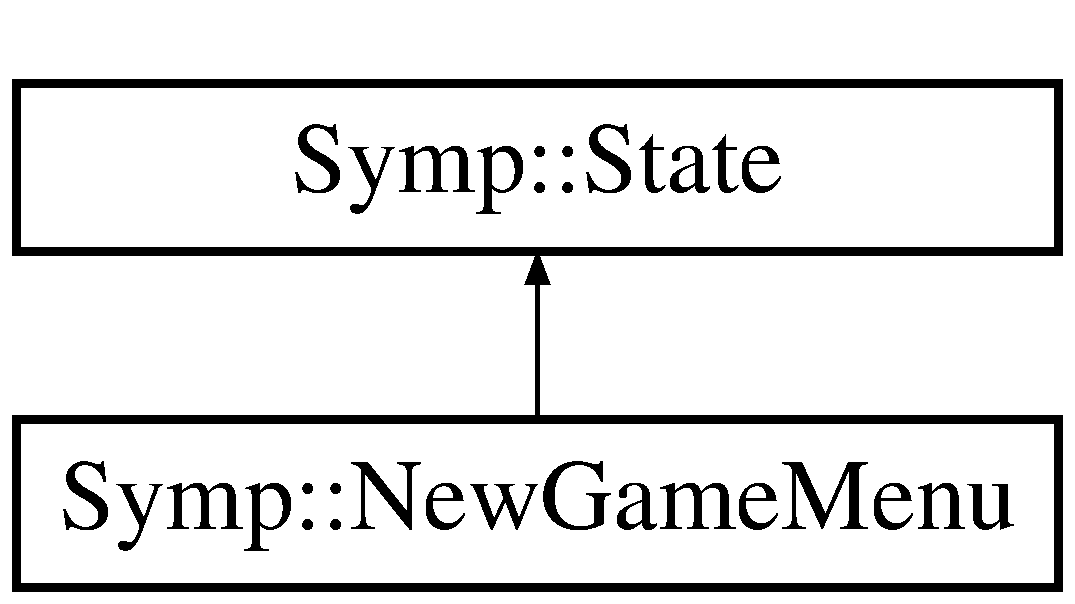
\includegraphics[height=2.000000cm]{class_symp_1_1_new_game_menu}
\end{center}
\end{figure}
\subsection*{Public Member Functions}
\begin{DoxyCompactItemize}
\item 
\hyperlink{class_symp_1_1_new_game_menu_abcb925e95443d461c296bf37ef42cd76}{New\-Game\-Menu} ()
\begin{DoxyCompactList}\small\item\em \hyperlink{class_symp_1_1_new_game_menu}{New\-Game\-Menu} constructor Responsible for the initialization of the private attributes of the \#\-New\-Game\-Menu\-Menu class. This function is not responsible for drawing the graphical elements that compose the menu, the \hyperlink{class_symp_1_1_new_game_menu_a8f57888361e8424acedda26143fd7746}{init()} function is. \end{DoxyCompactList}\item 
\hyperlink{class_symp_1_1_new_game_menu_a0ae319dc01e3244e6bcf2c5aa73b85bf}{$\sim$\-New\-Game\-Menu} ()
\item 
virtual void \hyperlink{class_symp_1_1_new_game_menu_a8f57888361e8424acedda26143fd7746}{init} ()
\begin{DoxyCompactList}\small\item\em \hyperlink{class_symp_1_1_new_game_menu}{New\-Game\-Menu} elements initialization The elements that compose the menu are created in this function. \end{DoxyCompactList}\item 
virtual void \hyperlink{class_symp_1_1_new_game_menu_a2e02c1b26f7e221de7a4cae2e856a41c}{handle\-Mouse\-Clic} (int mouse\-X, int mouse\-Y)
\begin{DoxyCompactList}\small\item\em Handle mouse clic events. \end{DoxyCompactList}\item 
virtual void \hyperlink{class_symp_1_1_new_game_menu_a4c52d19b89c3122ca989c2149467cdd2}{key\-Down\-Pressed} ()
\begin{DoxyCompactList}\small\item\em Handle key down event. \end{DoxyCompactList}\item 
virtual void \hyperlink{class_symp_1_1_new_game_menu_abb3d59240c9874026dd996bc9fb9a290}{key\-Up\-Pressed} ()
\begin{DoxyCompactList}\small\item\em Handle key up event. \end{DoxyCompactList}\item 
void \hyperlink{class_symp_1_1_new_game_menu_adb285b34356f42ec8dd9976b9eed666a}{receive\-Key\-Event} (std\-::string key)
\begin{DoxyCompactList}\small\item\em Handle key event for the \#\-Line\-Edit. \end{DoxyCompactList}\item 
void \hyperlink{class_symp_1_1_new_game_menu_a3d8810a072c5baff55c7580efa8152ea}{erase\-Previous\-Character} ()
\begin{DoxyCompactList}\small\item\em Erase the character which is before the cursor index. \end{DoxyCompactList}\item 
void \hyperlink{class_symp_1_1_new_game_menu_a9a5d8098dfff416824468045feb51d08}{erase\-Next\-Character} ()
\begin{DoxyCompactList}\small\item\em Erase the character which is after the cursor index. \end{DoxyCompactList}\item 
void \hyperlink{class_symp_1_1_new_game_menu_ade3a666ae49f6e671ac8ddfcba42b8ad}{move\-Cursor\-Left} ()
\begin{DoxyCompactList}\small\item\em Move the cursor of the \#\-Line\-Edit to the left. \end{DoxyCompactList}\item 
void \hyperlink{class_symp_1_1_new_game_menu_a76324c780657441e0ebd8a9ec8653532}{move\-Cursor\-Right} ()
\begin{DoxyCompactList}\small\item\em Move the cursor of the \#\-Line\-Edit to the right. \end{DoxyCompactList}\end{DoxyCompactItemize}


\subsection{Detailed Description}
the \hyperlink{class_symp_1_1_state_ad44d90b6e1b68eb021ceaa0cb98141a4}{State} interface for implementing the \hyperlink{class_symp_1_1_state}{State} Machine Pattern This Menu is the graphical interface for creating a new \#\-Player. The user can choose an avatar and type a name to register its \#\-Player. Then it can directly start a new game, or go back. \begin{DoxySeeAlso}{See Also}
\hyperlink{class_symp_1_1_state}{State} 

\hyperlink{class_symp_1_1_line_edit}{Line\-Edit} 

\hyperlink{class_symp_1_1_game_manager}{Game\-Manager} 

\hyperlink{class_symp_1_1_manage_games_menu}{Manage\-Games\-Menu} 

\hyperlink{class_symp_1_1_menu_manager}{Menu\-Manager} 
\end{DoxySeeAlso}


Definition at line 20 of file New\-Game\-Menu.\-h.



\subsection{Constructor \& Destructor Documentation}
\hypertarget{class_symp_1_1_new_game_menu_abcb925e95443d461c296bf37ef42cd76}{\index{Symp\-::\-New\-Game\-Menu@{Symp\-::\-New\-Game\-Menu}!New\-Game\-Menu@{New\-Game\-Menu}}
\index{New\-Game\-Menu@{New\-Game\-Menu}!Symp::NewGameMenu@{Symp\-::\-New\-Game\-Menu}}
\subsubsection[{New\-Game\-Menu}]{\setlength{\rightskip}{0pt plus 5cm}Symp\-::\-New\-Game\-Menu\-::\-New\-Game\-Menu (
\begin{DoxyParamCaption}
{}
\end{DoxyParamCaption}
)}}\label{class_symp_1_1_new_game_menu_abcb925e95443d461c296bf37ef42cd76}


\hyperlink{class_symp_1_1_new_game_menu}{New\-Game\-Menu} constructor Responsible for the initialization of the private attributes of the \#\-New\-Game\-Menu\-Menu class. This function is not responsible for drawing the graphical elements that compose the menu, the \hyperlink{class_symp_1_1_new_game_menu_a8f57888361e8424acedda26143fd7746}{init()} function is. 

\begin{DoxySeeAlso}{See Also}
\hyperlink{class_symp_1_1_player}{Player} 

\hyperlink{class_symp_1_1_menu_manager}{Menu\-Manager} 

\hyperlink{class_symp_1_1_state}{State} 

\hyperlink{class_symp_1_1_new_game_menu_a8f57888361e8424acedda26143fd7746}{init()} 

\hyperlink{class_symp_1_1_new_game_menu_a0ae319dc01e3244e6bcf2c5aa73b85bf}{$\sim$\-New\-Game\-Menu()} 
\end{DoxySeeAlso}


Definition at line 23 of file New\-Game\-Menu.\-cpp.

\hypertarget{class_symp_1_1_new_game_menu_a0ae319dc01e3244e6bcf2c5aa73b85bf}{\index{Symp\-::\-New\-Game\-Menu@{Symp\-::\-New\-Game\-Menu}!$\sim$\-New\-Game\-Menu@{$\sim$\-New\-Game\-Menu}}
\index{$\sim$\-New\-Game\-Menu@{$\sim$\-New\-Game\-Menu}!Symp::NewGameMenu@{Symp\-::\-New\-Game\-Menu}}
\subsubsection[{$\sim$\-New\-Game\-Menu}]{\setlength{\rightskip}{0pt plus 5cm}Symp\-::\-New\-Game\-Menu\-::$\sim$\-New\-Game\-Menu (
\begin{DoxyParamCaption}
{}
\end{DoxyParamCaption}
)\hspace{0.3cm}{\ttfamily [inline]}}}\label{class_symp_1_1_new_game_menu_a0ae319dc01e3244e6bcf2c5aa73b85bf}


Definition at line 23 of file New\-Game\-Menu.\-h.



\subsection{Member Function Documentation}
\hypertarget{class_symp_1_1_new_game_menu_a9a5d8098dfff416824468045feb51d08}{\index{Symp\-::\-New\-Game\-Menu@{Symp\-::\-New\-Game\-Menu}!erase\-Next\-Character@{erase\-Next\-Character}}
\index{erase\-Next\-Character@{erase\-Next\-Character}!Symp::NewGameMenu@{Symp\-::\-New\-Game\-Menu}}
\subsubsection[{erase\-Next\-Character}]{\setlength{\rightskip}{0pt plus 5cm}void Symp\-::\-New\-Game\-Menu\-::erase\-Next\-Character (
\begin{DoxyParamCaption}
{}
\end{DoxyParamCaption}
)}}\label{class_symp_1_1_new_game_menu_a9a5d8098dfff416824468045feb51d08}


Erase the character which is after the cursor index. 

\begin{DoxySeeAlso}{See Also}
\hyperlink{class_symp_1_1_menu_manager}{Menu\-Manager} 

\hyperlink{class_symp_1_1_state}{State} 

\hyperlink{class_symp_1_1_input_manager}{Input\-Manager} 

\hyperlink{class_symp_1_1_new_game_menu_a8f57888361e8424acedda26143fd7746}{init()} 
\end{DoxySeeAlso}


Definition at line 200 of file New\-Game\-Menu.\-cpp.

\hypertarget{class_symp_1_1_new_game_menu_a3d8810a072c5baff55c7580efa8152ea}{\index{Symp\-::\-New\-Game\-Menu@{Symp\-::\-New\-Game\-Menu}!erase\-Previous\-Character@{erase\-Previous\-Character}}
\index{erase\-Previous\-Character@{erase\-Previous\-Character}!Symp::NewGameMenu@{Symp\-::\-New\-Game\-Menu}}
\subsubsection[{erase\-Previous\-Character}]{\setlength{\rightskip}{0pt plus 5cm}void Symp\-::\-New\-Game\-Menu\-::erase\-Previous\-Character (
\begin{DoxyParamCaption}
{}
\end{DoxyParamCaption}
)}}\label{class_symp_1_1_new_game_menu_a3d8810a072c5baff55c7580efa8152ea}


Erase the character which is before the cursor index. 

\begin{DoxySeeAlso}{See Also}
\hyperlink{class_symp_1_1_menu_manager}{Menu\-Manager} 

\hyperlink{class_symp_1_1_state}{State} 

\hyperlink{class_symp_1_1_input_manager}{Input\-Manager} 

\hyperlink{class_symp_1_1_new_game_menu_a8f57888361e8424acedda26143fd7746}{init()} 
\end{DoxySeeAlso}


Definition at line 189 of file New\-Game\-Menu.\-cpp.

\hypertarget{class_symp_1_1_new_game_menu_a2e02c1b26f7e221de7a4cae2e856a41c}{\index{Symp\-::\-New\-Game\-Menu@{Symp\-::\-New\-Game\-Menu}!handle\-Mouse\-Clic@{handle\-Mouse\-Clic}}
\index{handle\-Mouse\-Clic@{handle\-Mouse\-Clic}!Symp::NewGameMenu@{Symp\-::\-New\-Game\-Menu}}
\subsubsection[{handle\-Mouse\-Clic}]{\setlength{\rightskip}{0pt plus 5cm}void Symp\-::\-New\-Game\-Menu\-::handle\-Mouse\-Clic (
\begin{DoxyParamCaption}
\item[{int}]{mouse\-X, }
\item[{int}]{mouse\-Y}
\end{DoxyParamCaption}
)\hspace{0.3cm}{\ttfamily [virtual]}}}\label{class_symp_1_1_new_game_menu_a2e02c1b26f7e221de7a4cae2e856a41c}


Handle mouse clic events. 


\begin{DoxyParams}{Parameters}
{\em mouse\-X} & the x coordinate of the mouse position \\
\hline
{\em mouse\-Y} & the y coordinate of the mouse position \\
\hline
\end{DoxyParams}
\begin{DoxySeeAlso}{See Also}
\hyperlink{class_symp_1_1_menu_manager}{Menu\-Manager} 

\hyperlink{class_symp_1_1_state}{State} 

\hyperlink{class_symp_1_1_input_manager}{Input\-Manager} 

\hyperlink{class_symp_1_1_new_game_menu_a8f57888361e8424acedda26143fd7746}{init()} 
\end{DoxySeeAlso}


Implements \hyperlink{class_symp_1_1_state_a23e468a10d9be4c79d17e22d1d5ef478}{Symp\-::\-State}.



Definition at line 130 of file New\-Game\-Menu.\-cpp.

\hypertarget{class_symp_1_1_new_game_menu_a8f57888361e8424acedda26143fd7746}{\index{Symp\-::\-New\-Game\-Menu@{Symp\-::\-New\-Game\-Menu}!init@{init}}
\index{init@{init}!Symp::NewGameMenu@{Symp\-::\-New\-Game\-Menu}}
\subsubsection[{init}]{\setlength{\rightskip}{0pt plus 5cm}void Symp\-::\-New\-Game\-Menu\-::init (
\begin{DoxyParamCaption}
{}
\end{DoxyParamCaption}
)\hspace{0.3cm}{\ttfamily [virtual]}}}\label{class_symp_1_1_new_game_menu_a8f57888361e8424acedda26143fd7746}


\hyperlink{class_symp_1_1_new_game_menu}{New\-Game\-Menu} elements initialization The elements that compose the menu are created in this function. 

\begin{DoxySeeAlso}{See Also}
\hyperlink{class_symp_1_1_player}{Player} 

\hyperlink{class_symp_1_1_menu_manager}{Menu\-Manager} 

\hyperlink{class_symp_1_1_state}{State} 

end() 

New\-Game\-Menu\-Menu() 
\end{DoxySeeAlso}


Implements \hyperlink{class_symp_1_1_state_a2c1c597b1235128a356c7529c42fdec3}{Symp\-::\-State}.



Definition at line 56 of file New\-Game\-Menu.\-cpp.

\hypertarget{class_symp_1_1_new_game_menu_a4c52d19b89c3122ca989c2149467cdd2}{\index{Symp\-::\-New\-Game\-Menu@{Symp\-::\-New\-Game\-Menu}!key\-Down\-Pressed@{key\-Down\-Pressed}}
\index{key\-Down\-Pressed@{key\-Down\-Pressed}!Symp::NewGameMenu@{Symp\-::\-New\-Game\-Menu}}
\subsubsection[{key\-Down\-Pressed}]{\setlength{\rightskip}{0pt plus 5cm}void Symp\-::\-New\-Game\-Menu\-::key\-Down\-Pressed (
\begin{DoxyParamCaption}
{}
\end{DoxyParamCaption}
)\hspace{0.3cm}{\ttfamily [virtual]}}}\label{class_symp_1_1_new_game_menu_a4c52d19b89c3122ca989c2149467cdd2}


Handle key down event. 

\begin{DoxySeeAlso}{See Also}
\hyperlink{class_symp_1_1_menu_manager}{Menu\-Manager} 

\hyperlink{class_symp_1_1_state}{State} 

\hyperlink{class_symp_1_1_input_manager}{Input\-Manager} 

\hyperlink{class_symp_1_1_new_game_menu_a8f57888361e8424acedda26143fd7746}{init()} 
\end{DoxySeeAlso}


Implements \hyperlink{class_symp_1_1_state_ac9ff920d185cdc17c9bc3ac63b40c62d}{Symp\-::\-State}.



Definition at line 233 of file New\-Game\-Menu.\-cpp.

\hypertarget{class_symp_1_1_new_game_menu_abb3d59240c9874026dd996bc9fb9a290}{\index{Symp\-::\-New\-Game\-Menu@{Symp\-::\-New\-Game\-Menu}!key\-Up\-Pressed@{key\-Up\-Pressed}}
\index{key\-Up\-Pressed@{key\-Up\-Pressed}!Symp::NewGameMenu@{Symp\-::\-New\-Game\-Menu}}
\subsubsection[{key\-Up\-Pressed}]{\setlength{\rightskip}{0pt plus 5cm}void Symp\-::\-New\-Game\-Menu\-::key\-Up\-Pressed (
\begin{DoxyParamCaption}
{}
\end{DoxyParamCaption}
)\hspace{0.3cm}{\ttfamily [virtual]}}}\label{class_symp_1_1_new_game_menu_abb3d59240c9874026dd996bc9fb9a290}


Handle key up event. 

\begin{DoxySeeAlso}{See Also}
\hyperlink{class_symp_1_1_menu_manager}{Menu\-Manager} 

\hyperlink{class_symp_1_1_state}{State} 

\hyperlink{class_symp_1_1_input_manager}{Input\-Manager} 

\hyperlink{class_symp_1_1_new_game_menu_a8f57888361e8424acedda26143fd7746}{init()} 
\end{DoxySeeAlso}


Implements \hyperlink{class_symp_1_1_state_a67d0fc2a02808bbcfdb06935c3be404f}{Symp\-::\-State}.



Definition at line 244 of file New\-Game\-Menu.\-cpp.

\hypertarget{class_symp_1_1_new_game_menu_ade3a666ae49f6e671ac8ddfcba42b8ad}{\index{Symp\-::\-New\-Game\-Menu@{Symp\-::\-New\-Game\-Menu}!move\-Cursor\-Left@{move\-Cursor\-Left}}
\index{move\-Cursor\-Left@{move\-Cursor\-Left}!Symp::NewGameMenu@{Symp\-::\-New\-Game\-Menu}}
\subsubsection[{move\-Cursor\-Left}]{\setlength{\rightskip}{0pt plus 5cm}void Symp\-::\-New\-Game\-Menu\-::move\-Cursor\-Left (
\begin{DoxyParamCaption}
{}
\end{DoxyParamCaption}
)}}\label{class_symp_1_1_new_game_menu_ade3a666ae49f6e671ac8ddfcba42b8ad}


Move the cursor of the \#\-Line\-Edit to the left. 

\begin{DoxySeeAlso}{See Also}
\hyperlink{class_symp_1_1_menu_manager}{Menu\-Manager} 

\hyperlink{class_symp_1_1_state}{State} 

\hyperlink{class_symp_1_1_input_manager}{Input\-Manager} 

\hyperlink{class_symp_1_1_new_game_menu_a8f57888361e8424acedda26143fd7746}{init()} 
\end{DoxySeeAlso}


Definition at line 211 of file New\-Game\-Menu.\-cpp.

\hypertarget{class_symp_1_1_new_game_menu_a76324c780657441e0ebd8a9ec8653532}{\index{Symp\-::\-New\-Game\-Menu@{Symp\-::\-New\-Game\-Menu}!move\-Cursor\-Right@{move\-Cursor\-Right}}
\index{move\-Cursor\-Right@{move\-Cursor\-Right}!Symp::NewGameMenu@{Symp\-::\-New\-Game\-Menu}}
\subsubsection[{move\-Cursor\-Right}]{\setlength{\rightskip}{0pt plus 5cm}void Symp\-::\-New\-Game\-Menu\-::move\-Cursor\-Right (
\begin{DoxyParamCaption}
{}
\end{DoxyParamCaption}
)}}\label{class_symp_1_1_new_game_menu_a76324c780657441e0ebd8a9ec8653532}


Move the cursor of the \#\-Line\-Edit to the right. 

\begin{DoxySeeAlso}{See Also}
\hyperlink{class_symp_1_1_menu_manager}{Menu\-Manager} 

\hyperlink{class_symp_1_1_state}{State} 

\hyperlink{class_symp_1_1_input_manager}{Input\-Manager} 

\hyperlink{class_symp_1_1_new_game_menu_a8f57888361e8424acedda26143fd7746}{init()} 
\end{DoxySeeAlso}


Definition at line 222 of file New\-Game\-Menu.\-cpp.

\hypertarget{class_symp_1_1_new_game_menu_adb285b34356f42ec8dd9976b9eed666a}{\index{Symp\-::\-New\-Game\-Menu@{Symp\-::\-New\-Game\-Menu}!receive\-Key\-Event@{receive\-Key\-Event}}
\index{receive\-Key\-Event@{receive\-Key\-Event}!Symp::NewGameMenu@{Symp\-::\-New\-Game\-Menu}}
\subsubsection[{receive\-Key\-Event}]{\setlength{\rightskip}{0pt plus 5cm}void Symp\-::\-New\-Game\-Menu\-::receive\-Key\-Event (
\begin{DoxyParamCaption}
\item[{std\-::string}]{key}
\end{DoxyParamCaption}
)}}\label{class_symp_1_1_new_game_menu_adb285b34356f42ec8dd9976b9eed666a}


Handle key event for the \#\-Line\-Edit. 

\begin{DoxySeeAlso}{See Also}
\hyperlink{class_symp_1_1_menu_manager}{Menu\-Manager} 

\hyperlink{class_symp_1_1_state}{State} 

\hyperlink{class_symp_1_1_input_manager}{Input\-Manager} 

\hyperlink{class_symp_1_1_new_game_menu_a8f57888361e8424acedda26143fd7746}{init()} 
\end{DoxySeeAlso}


Definition at line 178 of file New\-Game\-Menu.\-cpp.



The documentation for this class was generated from the following files\-:\begin{DoxyCompactItemize}
\item 
/home/cecilia/\-Documents/\-Symptogen/src/menu/\hyperlink{_new_game_menu_8h}{New\-Game\-Menu.\-h}\item 
/home/cecilia/\-Documents/\-Symptogen/src/menu/\hyperlink{_new_game_menu_8cpp}{New\-Game\-Menu.\-cpp}\end{DoxyCompactItemize}

\hypertarget{struct_symp_1_1_parser_collision}{\section{Symp\-:\-:Parser\-Collision Class Reference}
\label{struct_symp_1_1_parser_collision}\index{Symp\-::\-Parser\-Collision@{Symp\-::\-Parser\-Collision}}
}


{\ttfamily \#include $<$Parser\-Collision.\-h$>$}

Inheritance diagram for Symp\-:\-:Parser\-Collision\-:\begin{figure}[H]
\begin{center}
\leavevmode
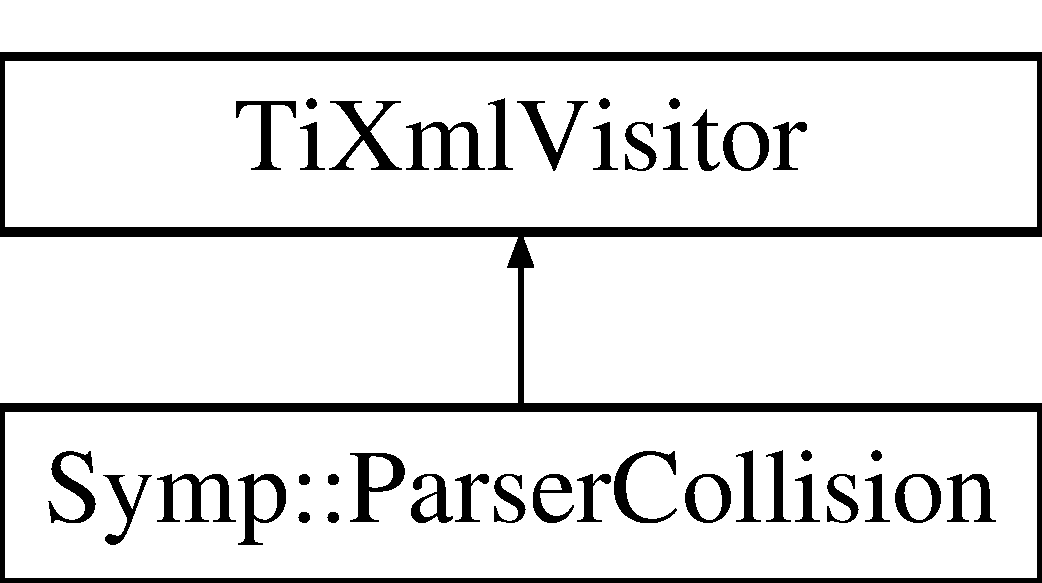
\includegraphics[height=2.000000cm]{struct_symp_1_1_parser_collision}
\end{center}
\end{figure}
\subsection*{Public Member Functions}
\begin{DoxyCompactItemize}
\item 
\hyperlink{struct_symp_1_1_parser_collision_aa399d593223247b92a46ff32771b467d}{Parser\-Collision} ()
\begin{DoxyCompactList}\small\item\em \hyperlink{struct_symp_1_1_parser_collision_aa399d593223247b92a46ff32771b467d}{Parser\-Collision} constructor. \end{DoxyCompactList}\item 
std\-::vector$<$ b2\-Vec2 $>$ \hyperlink{struct_symp_1_1_parser_collision_ad2e32aca1664bbb6166ae8f8ccee64fd}{load\-Collision} (const char $\ast$collision\-File\-Name, const b2\-Vec2 hit\-Box\-Dimensions)
\begin{DoxyCompactList}\small\item\em Load a level from an X\-M\-L file. \end{DoxyCompactList}\item 
bool \hyperlink{struct_symp_1_1_parser_collision_aea8246a25b90198580e3d9bd90b03a1e}{Visit\-Enter} (const Ti\-Xml\-Element \&element, const Ti\-Xml\-Attribute $\ast$attribute)
\begin{DoxyCompactList}\small\item\em Inherited from Tiny\-X\-M\-L Visitor class. This method is called when the visitor enters an X\-M\-L element. The main use of the \hyperlink{struct_symp_1_1_parser_collision_aea8246a25b90198580e3d9bd90b03a1e}{Visit\-Enter} method is to get the data into an X\-M\-L. It can be a \char`\"{}pure\char`\"{} data like position value or \char`\"{}state information\char`\"{} data like if the entity is on a physical layer. \end{DoxyCompactList}\item 
bool \hyperlink{struct_symp_1_1_parser_collision_ac1a8ff5684c792fed383b10e4045db41}{Visit\-Exit} (const Ti\-Xml\-Element \&element)
\begin{DoxyCompactList}\small\item\em Inherited from Tiny\-X\-M\-L Visitor class. This method is called when the visitor leaves an X\-M\-L element. The aim of the method is to create the different b2\-Vec2. \end{DoxyCompactList}\item 
void \hyperlink{struct_symp_1_1_parser_collision_a99a9c0b320eeecbeb09101300a87783d}{reset} (const b2\-Vec2 hitbox\-Dimension)
\end{DoxyCompactItemize}


\subsection{Detailed Description}
The \hyperlink{struct_symp_1_1_parser_collision_aa399d593223247b92a46ff32771b467d}{Parser\-Collision} class is responsible to read and load a level from a X\-M\-L file. It inherit from Ti\-Xml\-Visitor class. 

Definition at line 24 of file Parser\-Collision.\-h.



\subsection{Constructor \& Destructor Documentation}
\hypertarget{struct_symp_1_1_parser_collision_aa399d593223247b92a46ff32771b467d}{\index{Symp\-::\-Parser\-Collision@{Symp\-::\-Parser\-Collision}!Parser\-Collision@{Parser\-Collision}}
\index{Parser\-Collision@{Parser\-Collision}!Symp::ParserCollision@{Symp\-::\-Parser\-Collision}}
\subsubsection[{Parser\-Collision}]{\setlength{\rightskip}{0pt plus 5cm}Symp\-::\-Parser\-Collision\-::\-Parser\-Collision (
\begin{DoxyParamCaption}
{}
\end{DoxyParamCaption}
)}}\label{struct_symp_1_1_parser_collision_aa399d593223247b92a46ff32771b467d}


\hyperlink{struct_symp_1_1_parser_collision_aa399d593223247b92a46ff32771b467d}{Parser\-Collision} constructor. 



Definition at line 11 of file Parser\-Collision.\-cpp.



\subsection{Member Function Documentation}
\hypertarget{struct_symp_1_1_parser_collision_ad2e32aca1664bbb6166ae8f8ccee64fd}{\index{Symp\-::\-Parser\-Collision@{Symp\-::\-Parser\-Collision}!load\-Collision@{load\-Collision}}
\index{load\-Collision@{load\-Collision}!Symp::ParserCollision@{Symp\-::\-Parser\-Collision}}
\subsubsection[{load\-Collision}]{\setlength{\rightskip}{0pt plus 5cm}std\-::vector$<$ b2\-Vec2 $>$ Symp\-::\-Parser\-Collision\-::load\-Collision (
\begin{DoxyParamCaption}
\item[{const char $\ast$}]{collision\-File\-Name, }
\item[{const b2\-Vec2}]{hit\-Box\-Dimensions}
\end{DoxyParamCaption}
)}}\label{struct_symp_1_1_parser_collision_ad2e32aca1664bbb6166ae8f8ccee64fd}


Load a level from an X\-M\-L file. 


\begin{DoxyParams}{Parameters}
{\em map\-File\-Name} & \-: the name of the file to load \\
\hline
\end{DoxyParams}


Definition at line 19 of file Parser\-Collision.\-cpp.

\hypertarget{struct_symp_1_1_parser_collision_a99a9c0b320eeecbeb09101300a87783d}{\index{Symp\-::\-Parser\-Collision@{Symp\-::\-Parser\-Collision}!reset@{reset}}
\index{reset@{reset}!Symp::ParserCollision@{Symp\-::\-Parser\-Collision}}
\subsubsection[{reset}]{\setlength{\rightskip}{0pt plus 5cm}void Symp\-::\-Parser\-Collision\-::reset (
\begin{DoxyParamCaption}
\item[{const b2\-Vec2}]{hitbox\-Dimension}
\end{DoxyParamCaption}
)}}\label{struct_symp_1_1_parser_collision_a99a9c0b320eeecbeb09101300a87783d}
Clear the vector of vertices, and other data related to the previous shape. 

Definition at line 80 of file Parser\-Collision.\-cpp.

\hypertarget{struct_symp_1_1_parser_collision_aea8246a25b90198580e3d9bd90b03a1e}{\index{Symp\-::\-Parser\-Collision@{Symp\-::\-Parser\-Collision}!Visit\-Enter@{Visit\-Enter}}
\index{Visit\-Enter@{Visit\-Enter}!Symp::ParserCollision@{Symp\-::\-Parser\-Collision}}
\subsubsection[{Visit\-Enter}]{\setlength{\rightskip}{0pt plus 5cm}bool Symp\-::\-Parser\-Collision\-::\-Visit\-Enter (
\begin{DoxyParamCaption}
\item[{const Ti\-Xml\-Element \&}]{element, }
\item[{const Ti\-Xml\-Attribute $\ast$}]{attribute}
\end{DoxyParamCaption}
)}}\label{struct_symp_1_1_parser_collision_aea8246a25b90198580e3d9bd90b03a1e}


Inherited from Tiny\-X\-M\-L Visitor class. This method is called when the visitor enters an X\-M\-L element. The main use of the \hyperlink{struct_symp_1_1_parser_collision_aea8246a25b90198580e3d9bd90b03a1e}{Visit\-Enter} method is to get the data into an X\-M\-L. It can be a \char`\"{}pure\char`\"{} data like position value or \char`\"{}state information\char`\"{} data like if the entity is on a physical layer. 


\begin{DoxyParams}{Parameters}
{\em map\-File\-Name} & \-: the name of the file to load \\
\hline
\end{DoxyParams}


Definition at line 34 of file Parser\-Collision.\-cpp.

\hypertarget{struct_symp_1_1_parser_collision_ac1a8ff5684c792fed383b10e4045db41}{\index{Symp\-::\-Parser\-Collision@{Symp\-::\-Parser\-Collision}!Visit\-Exit@{Visit\-Exit}}
\index{Visit\-Exit@{Visit\-Exit}!Symp::ParserCollision@{Symp\-::\-Parser\-Collision}}
\subsubsection[{Visit\-Exit}]{\setlength{\rightskip}{0pt plus 5cm}bool Symp\-::\-Parser\-Collision\-::\-Visit\-Exit (
\begin{DoxyParamCaption}
\item[{const Ti\-Xml\-Element \&}]{element}
\end{DoxyParamCaption}
)}}\label{struct_symp_1_1_parser_collision_ac1a8ff5684c792fed383b10e4045db41}


Inherited from Tiny\-X\-M\-L Visitor class. This method is called when the visitor leaves an X\-M\-L element. The aim of the method is to create the different b2\-Vec2. 



Definition at line 63 of file Parser\-Collision.\-cpp.



The documentation for this class was generated from the following files\-:\begin{DoxyCompactItemize}
\item 
/home/cecilia/\-Documents/\-Symptogen/src/persistence/\hyperlink{_parser_collision_8h}{Parser\-Collision.\-h}\item 
/home/cecilia/\-Documents/\-Symptogen/src/persistence/\hyperlink{_parser_collision_8cpp}{Parser\-Collision.\-cpp}\end{DoxyCompactItemize}

\hypertarget{struct_symp_1_1_parser_level}{\section{Symp\-:\-:Parser\-Level Class Reference}
\label{struct_symp_1_1_parser_level}\index{Symp\-::\-Parser\-Level@{Symp\-::\-Parser\-Level}}
}


{\ttfamily \#include $<$Parser.\-h$>$}

Inheritance diagram for Symp\-:\-:Parser\-Level\-:\begin{figure}[H]
\begin{center}
\leavevmode
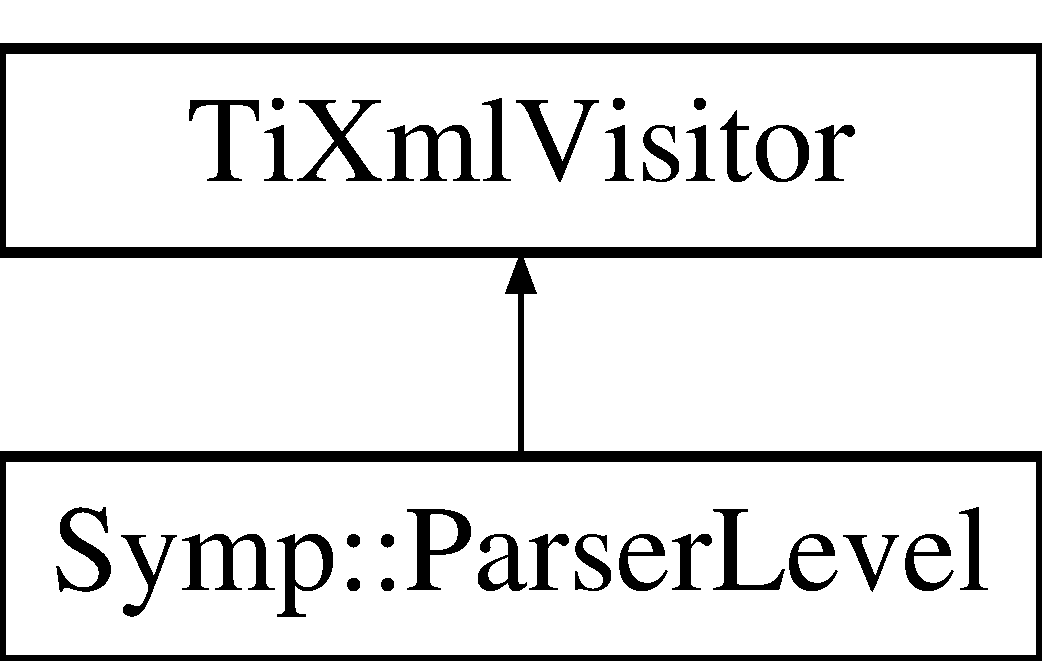
\includegraphics[height=2.000000cm]{struct_symp_1_1_parser_level}
\end{center}
\end{figure}
\subsection*{Public Member Functions}
\begin{DoxyCompactItemize}
\item 
\hyperlink{struct_symp_1_1_parser_level_a527575abc327361a4a3f6331d09a8ee5}{Parser\-Level} ()
\begin{DoxyCompactList}\small\item\em \hyperlink{struct_symp_1_1_parser_level_a527575abc327361a4a3f6331d09a8ee5}{Parser\-Level} constructor. \end{DoxyCompactList}\item 
float \hyperlink{struct_symp_1_1_parser_level_a73d3f7b58919f202224353b774440c12}{load\-Level} (const char $\ast$map\-File\-Name)
\begin{DoxyCompactList}\small\item\em Load a level from an X\-M\-L file. \end{DoxyCompactList}\item 
bool \hyperlink{struct_symp_1_1_parser_level_a4292eb4e5b4104543ef1b65b83b2d047}{Visit\-Enter} (const Ti\-Xml\-Element \&element, const Ti\-Xml\-Attribute $\ast$attribute)
\begin{DoxyCompactList}\small\item\em Inherited from Tiny\-X\-M\-L Visitor class. This method is called when the visitor enters an X\-M\-L element. The main use of the \hyperlink{struct_symp_1_1_parser_level_a4292eb4e5b4104543ef1b65b83b2d047}{Visit\-Enter} method is to get the data into an X\-M\-L. It can be a \char`\"{}pure\char`\"{} data like position value or \char`\"{}state information\char`\"{} data like if the entity is on a physical layer. \end{DoxyCompactList}\item 
bool \hyperlink{struct_symp_1_1_parser_level_a7d10cbbe06eb6f8b877d83b8b92d8c31}{Visit\-Exit} (const Ti\-Xml\-Element \&element)
\begin{DoxyCompactList}\small\item\em Inherited from Tiny\-X\-M\-L Visitor class. This method is called when the visitor leaves an X\-M\-L element. The aim of the method is to create the different entities depending on the \#\-Meta\-Entity data. \end{DoxyCompactList}\end{DoxyCompactItemize}


\subsection{Detailed Description}
The \hyperlink{struct_symp_1_1_parser_level_a527575abc327361a4a3f6331d09a8ee5}{Parser\-Level} class is responsible to read and load a level from a X\-M\-L file. It inherit from Ti\-Xml\-Visitor class. 

Definition at line 113 of file Parser.\-h.



\subsection{Constructor \& Destructor Documentation}
\hypertarget{struct_symp_1_1_parser_level_a527575abc327361a4a3f6331d09a8ee5}{\index{Symp\-::\-Parser\-Level@{Symp\-::\-Parser\-Level}!Parser\-Level@{Parser\-Level}}
\index{Parser\-Level@{Parser\-Level}!Symp::ParserLevel@{Symp\-::\-Parser\-Level}}
\subsubsection[{Parser\-Level}]{\setlength{\rightskip}{0pt plus 5cm}Symp\-::\-Parser\-Level\-::\-Parser\-Level (
\begin{DoxyParamCaption}
{}
\end{DoxyParamCaption}
)}}\label{struct_symp_1_1_parser_level_a527575abc327361a4a3f6331d09a8ee5}


\hyperlink{struct_symp_1_1_parser_level_a527575abc327361a4a3f6331d09a8ee5}{Parser\-Level} constructor. 



Definition at line 41 of file Parser.\-cpp.



\subsection{Member Function Documentation}
\hypertarget{struct_symp_1_1_parser_level_a73d3f7b58919f202224353b774440c12}{\index{Symp\-::\-Parser\-Level@{Symp\-::\-Parser\-Level}!load\-Level@{load\-Level}}
\index{load\-Level@{load\-Level}!Symp::ParserLevel@{Symp\-::\-Parser\-Level}}
\subsubsection[{load\-Level}]{\setlength{\rightskip}{0pt plus 5cm}float Symp\-::\-Parser\-Level\-::load\-Level (
\begin{DoxyParamCaption}
\item[{const char $\ast$}]{map\-File\-Name}
\end{DoxyParamCaption}
)}}\label{struct_symp_1_1_parser_level_a73d3f7b58919f202224353b774440c12}


Load a level from an X\-M\-L file. 


\begin{DoxyParams}{Parameters}
{\em map\-File\-Name} & \-: the name of the file to load \\
\hline
\end{DoxyParams}
\begin{DoxyReturn}{Returns}
value to set the zoom of the game in \hyperlink{class_symp_1_1_game_manager}{Game\-Manager} 
\end{DoxyReturn}


Definition at line 46 of file Parser.\-cpp.

\hypertarget{struct_symp_1_1_parser_level_a4292eb4e5b4104543ef1b65b83b2d047}{\index{Symp\-::\-Parser\-Level@{Symp\-::\-Parser\-Level}!Visit\-Enter@{Visit\-Enter}}
\index{Visit\-Enter@{Visit\-Enter}!Symp::ParserLevel@{Symp\-::\-Parser\-Level}}
\subsubsection[{Visit\-Enter}]{\setlength{\rightskip}{0pt plus 5cm}bool Symp\-::\-Parser\-Level\-::\-Visit\-Enter (
\begin{DoxyParamCaption}
\item[{const Ti\-Xml\-Element \&}]{element, }
\item[{const Ti\-Xml\-Attribute $\ast$}]{attribute}
\end{DoxyParamCaption}
)}}\label{struct_symp_1_1_parser_level_a4292eb4e5b4104543ef1b65b83b2d047}


Inherited from Tiny\-X\-M\-L Visitor class. This method is called when the visitor enters an X\-M\-L element. The main use of the \hyperlink{struct_symp_1_1_parser_level_a4292eb4e5b4104543ef1b65b83b2d047}{Visit\-Enter} method is to get the data into an X\-M\-L. It can be a \char`\"{}pure\char`\"{} data like position value or \char`\"{}state information\char`\"{} data like if the entity is on a physical layer. 


\begin{DoxyParams}{Parameters}
{\em map\-File\-Name} & \-: the name of the file to load \\
\hline
\end{DoxyParams}


Definition at line 75 of file Parser.\-cpp.

\hypertarget{struct_symp_1_1_parser_level_a7d10cbbe06eb6f8b877d83b8b92d8c31}{\index{Symp\-::\-Parser\-Level@{Symp\-::\-Parser\-Level}!Visit\-Exit@{Visit\-Exit}}
\index{Visit\-Exit@{Visit\-Exit}!Symp::ParserLevel@{Symp\-::\-Parser\-Level}}
\subsubsection[{Visit\-Exit}]{\setlength{\rightskip}{0pt plus 5cm}bool Symp\-::\-Parser\-Level\-::\-Visit\-Exit (
\begin{DoxyParamCaption}
\item[{const Ti\-Xml\-Element \&}]{element}
\end{DoxyParamCaption}
)}}\label{struct_symp_1_1_parser_level_a7d10cbbe06eb6f8b877d83b8b92d8c31}


Inherited from Tiny\-X\-M\-L Visitor class. This method is called when the visitor leaves an X\-M\-L element. The aim of the method is to create the different entities depending on the \#\-Meta\-Entity data. 



Definition at line 239 of file Parser.\-cpp.



The documentation for this class was generated from the following files\-:\begin{DoxyCompactItemize}
\item 
/home/cecilia/\-Documents/\-Symptogen/src/persistence/\hyperlink{_parser_8h}{Parser.\-h}\item 
/home/cecilia/\-Documents/\-Symptogen/src/persistence/\hyperlink{_parser_8cpp}{Parser.\-cpp}\end{DoxyCompactItemize}

\hypertarget{class_symp_1_1_parser_player}{\section{Symp\-:\-:Parser\-Player Class Reference}
\label{class_symp_1_1_parser_player}\index{Symp\-::\-Parser\-Player@{Symp\-::\-Parser\-Player}}
}


{\ttfamily \#include $<$Parser.\-h$>$}

\subsection*{Public Member Functions}
\begin{DoxyCompactItemize}
\item 
\hyperlink{class_symp_1_1_parser_player_a03f3dfe4d73a8dadb71ae5fd034bc9bc}{Parser\-Player} (std\-::string s\-Player\-Data\-Path)
\begin{DoxyCompactList}\small\item\em \hyperlink{class_symp_1_1_parser_player_a03f3dfe4d73a8dadb71ae5fd034bc9bc}{Parser\-Player} constructor. \end{DoxyCompactList}\item 
\hyperlink{class_symp_1_1_parser_player_a418e3d0bbe4bb706b6d66aeb903fb9c1}{$\sim$\-Parser\-Player} ()
\begin{DoxyCompactList}\small\item\em \hyperlink{class_symp_1_1_parser_player_a03f3dfe4d73a8dadb71ae5fd034bc9bc}{Parser\-Player} destructor. \end{DoxyCompactList}\item 
std\-::pair$<$ \hyperlink{class_symp_1_1_player}{Player} \\*
$\ast$, std\-::vector$<$ \hyperlink{class_symp_1_1_player}{Player} $\ast$ $>$ $>$ \hyperlink{class_symp_1_1_parser_player_a5557f2a1924c72138e9a865e46e64d9a}{load\-Player\-Data} ()
\begin{DoxyCompactList}\small\item\em Load persistent data from an X\-M\-L file. This method read the content of an X\-M\-L file and create the differents players games. The current player is defined into the file. \end{DoxyCompactList}\item 
void \hyperlink{class_symp_1_1_parser_player_a5b631d7764c94970f29b3b5aaa20a55f}{save\-Player\-Data} (std\-::pair$<$ \hyperlink{class_symp_1_1_player}{Player} $\ast$, std\-::vector$<$ \hyperlink{class_symp_1_1_player}{Player} $\ast$ $>$$>$ player\-Data)
\begin{DoxyCompactList}\small\item\em Save the input \#\-Player datas into an X\-M\-L file. \end{DoxyCompactList}\end{DoxyCompactItemize}


\subsection{Detailed Description}
The \hyperlink{class_symp_1_1_parser_player_a03f3dfe4d73a8dadb71ae5fd034bc9bc}{Parser\-Player} class is responsible the reading and writtent of xml exernal data. Its main use is to manage the \#\-Player data. The \hyperlink{class_symp_1_1_parser_player_a03f3dfe4d73a8dadb71ae5fd034bc9bc}{Parser\-Player} use the Tiny\-X\-M\-L library. \begin{DoxySeeAlso}{See Also}
\hyperlink{class_symp_1_1_game_manager}{Game\-Manager} 

\hyperlink{class_symp_1_1_player}{Player} 
\end{DoxySeeAlso}


Definition at line 193 of file Parser.\-h.



\subsection{Constructor \& Destructor Documentation}
\hypertarget{class_symp_1_1_parser_player_a03f3dfe4d73a8dadb71ae5fd034bc9bc}{\index{Symp\-::\-Parser\-Player@{Symp\-::\-Parser\-Player}!Parser\-Player@{Parser\-Player}}
\index{Parser\-Player@{Parser\-Player}!Symp::ParserPlayer@{Symp\-::\-Parser\-Player}}
\subsubsection[{Parser\-Player}]{\setlength{\rightskip}{0pt plus 5cm}Symp\-::\-Parser\-Player\-::\-Parser\-Player (
\begin{DoxyParamCaption}
\item[{std\-::string}]{s\-Player\-Data\-Path}
\end{DoxyParamCaption}
)}}\label{class_symp_1_1_parser_player_a03f3dfe4d73a8dadb71ae5fd034bc9bc}


\hyperlink{class_symp_1_1_parser_player_a03f3dfe4d73a8dadb71ae5fd034bc9bc}{Parser\-Player} constructor. 

\hyperlink{class_symp_1_1_parser_player}{Parser\-Player} constructor.


\begin{DoxyParams}{Parameters}
{\em s\-Player\-Data\-Path} & the relative path to the xml file that contain the player's data \\
\hline
\end{DoxyParams}
\begin{DoxySeeAlso}{See Also}
\hyperlink{class_symp_1_1_game_manager}{Game\-Manager} 

\hyperlink{class_symp_1_1_parser_player_a418e3d0bbe4bb706b6d66aeb903fb9c1}{$\sim$\-Parser\-Player()} 

\hyperlink{class_symp_1_1_player}{Player} 
\end{DoxySeeAlso}


Definition at line 487 of file Parser.\-cpp.

\hypertarget{class_symp_1_1_parser_player_a418e3d0bbe4bb706b6d66aeb903fb9c1}{\index{Symp\-::\-Parser\-Player@{Symp\-::\-Parser\-Player}!$\sim$\-Parser\-Player@{$\sim$\-Parser\-Player}}
\index{$\sim$\-Parser\-Player@{$\sim$\-Parser\-Player}!Symp::ParserPlayer@{Symp\-::\-Parser\-Player}}
\subsubsection[{$\sim$\-Parser\-Player}]{\setlength{\rightskip}{0pt plus 5cm}Symp\-::\-Parser\-Player\-::$\sim$\-Parser\-Player (
\begin{DoxyParamCaption}
{}
\end{DoxyParamCaption}
)\hspace{0.3cm}{\ttfamily [inline]}}}\label{class_symp_1_1_parser_player_a418e3d0bbe4bb706b6d66aeb903fb9c1}


\hyperlink{class_symp_1_1_parser_player_a03f3dfe4d73a8dadb71ae5fd034bc9bc}{Parser\-Player} destructor. 



Definition at line 205 of file Parser.\-h.



\subsection{Member Function Documentation}
\hypertarget{class_symp_1_1_parser_player_a5557f2a1924c72138e9a865e46e64d9a}{\index{Symp\-::\-Parser\-Player@{Symp\-::\-Parser\-Player}!load\-Player\-Data@{load\-Player\-Data}}
\index{load\-Player\-Data@{load\-Player\-Data}!Symp::ParserPlayer@{Symp\-::\-Parser\-Player}}
\subsubsection[{load\-Player\-Data}]{\setlength{\rightskip}{0pt plus 5cm}std\-::pair$<$ {\bf Player} $\ast$, std\-::vector$<$ {\bf Player} $\ast$ $>$ $>$ Symp\-::\-Parser\-Player\-::load\-Player\-Data (
\begin{DoxyParamCaption}
{}
\end{DoxyParamCaption}
)}}\label{class_symp_1_1_parser_player_a5557f2a1924c72138e9a865e46e64d9a}


Load persistent data from an X\-M\-L file. This method read the content of an X\-M\-L file and create the differents players games. The current player is defined into the file. 

Load the player data from the xml file.

\begin{DoxyReturn}{Returns}
a pair $<$\#\-Player$\ast$, std\-::vector$<$\#\-Player$\ast$$>$$>$. The first component is the current player and the vector of \#\-Player$\ast$ is corresponding to the list of the other players.

std\-::pair a std\-::pair that contain the last player and the vector of the others players 
\end{DoxyReturn}
\begin{DoxySeeAlso}{See Also}
\hyperlink{class_symp_1_1_parser_player}{Parser\-Player} 

\hyperlink{class_symp_1_1_parser_player_a418e3d0bbe4bb706b6d66aeb903fb9c1}{$\sim$\-Parser\-Player()} 

\hyperlink{class_symp_1_1_parser_player_a5b631d7764c94970f29b3b5aaa20a55f}{save\-Player\-Data()} 

\hyperlink{class_symp_1_1_player}{Player} 
\end{DoxySeeAlso}


Definition at line 499 of file Parser.\-cpp.

\hypertarget{class_symp_1_1_parser_player_a5b631d7764c94970f29b3b5aaa20a55f}{\index{Symp\-::\-Parser\-Player@{Symp\-::\-Parser\-Player}!save\-Player\-Data@{save\-Player\-Data}}
\index{save\-Player\-Data@{save\-Player\-Data}!Symp::ParserPlayer@{Symp\-::\-Parser\-Player}}
\subsubsection[{save\-Player\-Data}]{\setlength{\rightskip}{0pt plus 5cm}void Symp\-::\-Parser\-Player\-::save\-Player\-Data (
\begin{DoxyParamCaption}
\item[{std\-::pair$<$ {\bf Player} $\ast$, std\-::vector$<$ {\bf Player} $\ast$ $>$$>$}]{player\-Data}
\end{DoxyParamCaption}
)}}\label{class_symp_1_1_parser_player_a5b631d7764c94970f29b3b5aaa20a55f}


Save the input \#\-Player datas into an X\-M\-L file. 

Save the player's data into a xml file.


\begin{DoxyParams}{Parameters}
{\em player\-Data} & \-: a pair of $<$\#\-Player$\ast$, std\-::vector$<$\#\-Player$\ast$$>$$>$. The first component is corresponding to the current player and the vector of \#\-Player$\ast$ is corresponding to the list of the other players.\\
\hline
{\em player\-Data} & a std\-::pair that contain the last player and the vector of the others players \\
\hline
\end{DoxyParams}
\begin{DoxySeeAlso}{See Also}
\hyperlink{class_symp_1_1_parser_player}{Parser\-Player} 

\hyperlink{class_symp_1_1_parser_player_a418e3d0bbe4bb706b6d66aeb903fb9c1}{$\sim$\-Parser\-Player()} 

\hyperlink{class_symp_1_1_parser_player_a5557f2a1924c72138e9a865e46e64d9a}{load\-Player\-Data()} 

\hyperlink{class_symp_1_1_player}{Player} 
\end{DoxySeeAlso}


Definition at line 547 of file Parser.\-cpp.



The documentation for this class was generated from the following files\-:\begin{DoxyCompactItemize}
\item 
/home/cecilia/\-Documents/\-Symptogen/src/persistence/\hyperlink{_parser_8h}{Parser.\-h}\item 
/home/cecilia/\-Documents/\-Symptogen/src/persistence/\hyperlink{_parser_8cpp}{Parser.\-cpp}\end{DoxyCompactItemize}

\hypertarget{class_symp_1_1_pause_menu}{\section{Symp\-:\-:Pause\-Menu Class Reference}
\label{class_symp_1_1_pause_menu}\index{Symp\-::\-Pause\-Menu@{Symp\-::\-Pause\-Menu}}
}


{\ttfamily \#include $<$Pause\-Menu.\-h$>$}

Inheritance diagram for Symp\-:\-:Pause\-Menu\-:\begin{figure}[H]
\begin{center}
\leavevmode
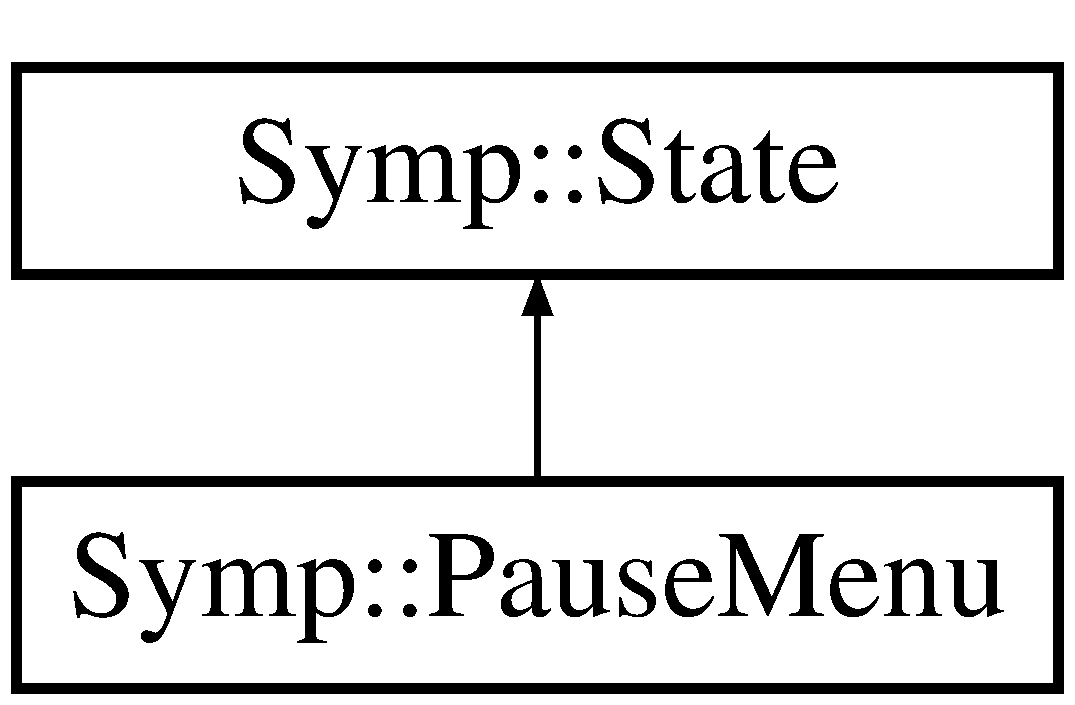
\includegraphics[height=2.000000cm]{class_symp_1_1_pause_menu}
\end{center}
\end{figure}
\subsection*{Public Member Functions}
\begin{DoxyCompactItemize}
\item 
\hyperlink{class_symp_1_1_pause_menu_a2b33d027cab75b41f900d4015b314916}{Pause\-Menu} (float pos\-X, float pos\-Y)
\begin{DoxyCompactList}\small\item\em \hyperlink{class_symp_1_1_pause_menu}{Pause\-Menu} constructor Responsible for the initialization of the private attributes of the \#\-Pause\-Menu\-Menu class. \end{DoxyCompactList}\item 
\hyperlink{class_symp_1_1_pause_menu_a4f960c6e1b391025fc64a59e65fd2f73}{$\sim$\-Pause\-Menu} ()
\begin{DoxyCompactList}\small\item\em \hyperlink{class_symp_1_1_pause_menu}{Pause\-Menu} destructor Responsible for telling the \#\-Menu\-Manager that the pause is no longer required, so the \#\-Game\-Manager will update the application. \end{DoxyCompactList}\item 
virtual void \hyperlink{class_symp_1_1_pause_menu_af456bb275fc71d5a9ee3290e5d82cd90}{init} ()
\begin{DoxyCompactList}\small\item\em \hyperlink{class_symp_1_1_pause_menu}{Pause\-Menu} elements initialization The elements that compose the menu are created in this function. \end{DoxyCompactList}\item 
virtual void \hyperlink{class_symp_1_1_pause_menu_a2a4fd25c988e7b2db561af0f76449cda}{handle\-Mouse\-Clic} (int mouse\-X, int mouse\-Y)
\begin{DoxyCompactList}\small\item\em Handle mouse clic events. \end{DoxyCompactList}\item 
virtual void \hyperlink{class_symp_1_1_pause_menu_af20fcbac9585f1e34eef8de5c84bf9e3}{key\-Down\-Pressed} ()
\begin{DoxyCompactList}\small\item\em Handle key down event. \end{DoxyCompactList}\item 
virtual void \hyperlink{class_symp_1_1_pause_menu_ab6329d721b22dfb991e794768e0d5afd}{key\-Up\-Pressed} ()
\begin{DoxyCompactList}\small\item\em Handle key up event. \end{DoxyCompactList}\end{DoxyCompactItemize}


\subsection{Detailed Description}
the \hyperlink{class_symp_1_1_state_ad44d90b6e1b68eb021ceaa0cb98141a4}{State} interface for implementing the \hyperlink{class_symp_1_1_state}{State} Machine Pattern This Menu is the only in game menu. It appears while the player is in a game, on the escape key event. This class is directly managed by the \#\-Game\-Manager for it is appearing in the middle of the game. The user can from this menu restart a level, quit the game to display the main menu or resume its game. \begin{DoxySeeAlso}{See Also}
\hyperlink{class_symp_1_1_state}{State} 

\hyperlink{class_symp_1_1_game_manager}{Game\-Manager} 

\hyperlink{class_symp_1_1_welcome_last_player_menu}{Welcome\-Last\-Player\-Menu} 

\hyperlink{class_symp_1_1_menu_manager}{Menu\-Manager} 
\end{DoxySeeAlso}


Definition at line 19 of file Pause\-Menu.\-h.



\subsection{Constructor \& Destructor Documentation}
\hypertarget{class_symp_1_1_pause_menu_a2b33d027cab75b41f900d4015b314916}{\index{Symp\-::\-Pause\-Menu@{Symp\-::\-Pause\-Menu}!Pause\-Menu@{Pause\-Menu}}
\index{Pause\-Menu@{Pause\-Menu}!Symp::PauseMenu@{Symp\-::\-Pause\-Menu}}
\subsubsection[{Pause\-Menu}]{\setlength{\rightskip}{0pt plus 5cm}Symp\-::\-Pause\-Menu\-::\-Pause\-Menu (
\begin{DoxyParamCaption}
\item[{float}]{pos\-X, }
\item[{float}]{pos\-Y}
\end{DoxyParamCaption}
)}}\label{class_symp_1_1_pause_menu_a2b33d027cab75b41f900d4015b314916}


\hyperlink{class_symp_1_1_pause_menu}{Pause\-Menu} constructor Responsible for the initialization of the private attributes of the \#\-Pause\-Menu\-Menu class. 

\begin{DoxySeeAlso}{See Also}
\hyperlink{class_symp_1_1_menu_manager}{Menu\-Manager} 

\hyperlink{class_symp_1_1_state}{State} 

\hyperlink{class_symp_1_1_pause_menu_af456bb275fc71d5a9ee3290e5d82cd90}{init()} 

$\sim$\-Pause\-Menu\-Menu() 
\end{DoxySeeAlso}


Definition at line 18 of file Pause\-Menu.\-cpp.

\hypertarget{class_symp_1_1_pause_menu_a4f960c6e1b391025fc64a59e65fd2f73}{\index{Symp\-::\-Pause\-Menu@{Symp\-::\-Pause\-Menu}!$\sim$\-Pause\-Menu@{$\sim$\-Pause\-Menu}}
\index{$\sim$\-Pause\-Menu@{$\sim$\-Pause\-Menu}!Symp::PauseMenu@{Symp\-::\-Pause\-Menu}}
\subsubsection[{$\sim$\-Pause\-Menu}]{\setlength{\rightskip}{0pt plus 5cm}Symp\-::\-Pause\-Menu\-::$\sim$\-Pause\-Menu (
\begin{DoxyParamCaption}
{}
\end{DoxyParamCaption}
)}}\label{class_symp_1_1_pause_menu_a4f960c6e1b391025fc64a59e65fd2f73}


\hyperlink{class_symp_1_1_pause_menu}{Pause\-Menu} destructor Responsible for telling the \#\-Menu\-Manager that the pause is no longer required, so the \#\-Game\-Manager will update the application. 

\begin{DoxySeeAlso}{See Also}
\hyperlink{class_symp_1_1_menu_manager}{Menu\-Manager} 

\hyperlink{class_symp_1_1_state}{State} 

\hyperlink{class_symp_1_1_pause_menu_af456bb275fc71d5a9ee3290e5d82cd90}{init()} 
\end{DoxySeeAlso}


Definition at line 32 of file Pause\-Menu.\-cpp.



\subsection{Member Function Documentation}
\hypertarget{class_symp_1_1_pause_menu_a2a4fd25c988e7b2db561af0f76449cda}{\index{Symp\-::\-Pause\-Menu@{Symp\-::\-Pause\-Menu}!handle\-Mouse\-Clic@{handle\-Mouse\-Clic}}
\index{handle\-Mouse\-Clic@{handle\-Mouse\-Clic}!Symp::PauseMenu@{Symp\-::\-Pause\-Menu}}
\subsubsection[{handle\-Mouse\-Clic}]{\setlength{\rightskip}{0pt plus 5cm}void Symp\-::\-Pause\-Menu\-::handle\-Mouse\-Clic (
\begin{DoxyParamCaption}
\item[{int}]{mouse\-X, }
\item[{int}]{mouse\-Y}
\end{DoxyParamCaption}
)\hspace{0.3cm}{\ttfamily [virtual]}}}\label{class_symp_1_1_pause_menu_a2a4fd25c988e7b2db561af0f76449cda}


Handle mouse clic events. 


\begin{DoxyParams}{Parameters}
{\em mouse\-X} & the x coordinate of the mouse position \\
\hline
{\em mouse\-Y} & the y coordinate of the mouse position \\
\hline
\end{DoxyParams}
\begin{DoxySeeAlso}{See Also}
\hyperlink{class_symp_1_1_menu_manager}{Menu\-Manager} 

\hyperlink{class_symp_1_1_state}{State} 

\hyperlink{class_symp_1_1_input_manager}{Input\-Manager} 

\hyperlink{class_symp_1_1_pause_menu_af456bb275fc71d5a9ee3290e5d82cd90}{init()} 
\end{DoxySeeAlso}


Implements \hyperlink{class_symp_1_1_state_a23e468a10d9be4c79d17e22d1d5ef478}{Symp\-::\-State}.



Definition at line 101 of file Pause\-Menu.\-cpp.

\hypertarget{class_symp_1_1_pause_menu_af456bb275fc71d5a9ee3290e5d82cd90}{\index{Symp\-::\-Pause\-Menu@{Symp\-::\-Pause\-Menu}!init@{init}}
\index{init@{init}!Symp::PauseMenu@{Symp\-::\-Pause\-Menu}}
\subsubsection[{init}]{\setlength{\rightskip}{0pt plus 5cm}void Symp\-::\-Pause\-Menu\-::init (
\begin{DoxyParamCaption}
{}
\end{DoxyParamCaption}
)\hspace{0.3cm}{\ttfamily [virtual]}}}\label{class_symp_1_1_pause_menu_af456bb275fc71d5a9ee3290e5d82cd90}


\hyperlink{class_symp_1_1_pause_menu}{Pause\-Menu} elements initialization The elements that compose the menu are created in this function. 

\begin{DoxySeeAlso}{See Also}
\hyperlink{class_symp_1_1_player}{Player} 

\hyperlink{class_symp_1_1_menu_manager}{Menu\-Manager} 

\hyperlink{class_symp_1_1_state}{State} 

end() 

\hyperlink{class_symp_1_1_pause_menu_a2b33d027cab75b41f900d4015b314916}{Pause\-Menu()} 
\end{DoxySeeAlso}


Implements \hyperlink{class_symp_1_1_state_a2c1c597b1235128a356c7529c42fdec3}{Symp\-::\-State}.



Definition at line 46 of file Pause\-Menu.\-cpp.

\hypertarget{class_symp_1_1_pause_menu_af20fcbac9585f1e34eef8de5c84bf9e3}{\index{Symp\-::\-Pause\-Menu@{Symp\-::\-Pause\-Menu}!key\-Down\-Pressed@{key\-Down\-Pressed}}
\index{key\-Down\-Pressed@{key\-Down\-Pressed}!Symp::PauseMenu@{Symp\-::\-Pause\-Menu}}
\subsubsection[{key\-Down\-Pressed}]{\setlength{\rightskip}{0pt plus 5cm}void Symp\-::\-Pause\-Menu\-::key\-Down\-Pressed (
\begin{DoxyParamCaption}
{}
\end{DoxyParamCaption}
)\hspace{0.3cm}{\ttfamily [virtual]}}}\label{class_symp_1_1_pause_menu_af20fcbac9585f1e34eef8de5c84bf9e3}


Handle key down event. 

\begin{DoxySeeAlso}{See Also}
\hyperlink{class_symp_1_1_menu_manager}{Menu\-Manager} 

\hyperlink{class_symp_1_1_state}{State} 

\hyperlink{class_symp_1_1_input_manager}{Input\-Manager} 

\hyperlink{class_symp_1_1_pause_menu_af456bb275fc71d5a9ee3290e5d82cd90}{init()} 
\end{DoxySeeAlso}


Implements \hyperlink{class_symp_1_1_state_ac9ff920d185cdc17c9bc3ac63b40c62d}{Symp\-::\-State}.



Definition at line 122 of file Pause\-Menu.\-cpp.

\hypertarget{class_symp_1_1_pause_menu_ab6329d721b22dfb991e794768e0d5afd}{\index{Symp\-::\-Pause\-Menu@{Symp\-::\-Pause\-Menu}!key\-Up\-Pressed@{key\-Up\-Pressed}}
\index{key\-Up\-Pressed@{key\-Up\-Pressed}!Symp::PauseMenu@{Symp\-::\-Pause\-Menu}}
\subsubsection[{key\-Up\-Pressed}]{\setlength{\rightskip}{0pt plus 5cm}void Symp\-::\-Pause\-Menu\-::key\-Up\-Pressed (
\begin{DoxyParamCaption}
{}
\end{DoxyParamCaption}
)\hspace{0.3cm}{\ttfamily [virtual]}}}\label{class_symp_1_1_pause_menu_ab6329d721b22dfb991e794768e0d5afd}


Handle key up event. 

\begin{DoxySeeAlso}{See Also}
\hyperlink{class_symp_1_1_menu_manager}{Menu\-Manager} 

\hyperlink{class_symp_1_1_state}{State} 

\hyperlink{class_symp_1_1_input_manager}{Input\-Manager} 

\hyperlink{class_symp_1_1_pause_menu_af456bb275fc71d5a9ee3290e5d82cd90}{init()} 
\end{DoxySeeAlso}


Implements \hyperlink{class_symp_1_1_state_a67d0fc2a02808bbcfdb06935c3be404f}{Symp\-::\-State}.



Definition at line 133 of file Pause\-Menu.\-cpp.



The documentation for this class was generated from the following files\-:\begin{DoxyCompactItemize}
\item 
/home/cecilia/\-Documents/\-Symptogen/src/menu/\hyperlink{_pause_menu_8h}{Pause\-Menu.\-h}\item 
/home/cecilia/\-Documents/\-Symptogen/src/menu/\hyperlink{_pause_menu_8cpp}{Pause\-Menu.\-cpp}\end{DoxyCompactItemize}

\hypertarget{class_symp_1_1_physical_entity}{\section{Symp\-:\-:Physical\-Entity Class Reference}
\label{class_symp_1_1_physical_entity}\index{Symp\-::\-Physical\-Entity@{Symp\-::\-Physical\-Entity}}
}


{\ttfamily \#include $<$Physical\-Entity.\-h$>$}

\subsection*{Public Member Functions}
\begin{DoxyCompactItemize}
\item 
\hyperlink{class_symp_1_1_physical_entity_a525034641510b5b899dcf1ad100e2af5}{Physical\-Entity} (b2\-World $\ast$world, const b2\-Vec2 origin, const b2\-Vec2 hit\-Box\-Dimensions, const \hyperlink{namespace_symp_aebf0e58b2f3c80a5dfa3ddbe64ace7e5}{Physical\-Type} physical\-Type)
\begin{DoxyCompactList}\small\item\em Create a physical entity, which use Box2\-D to manage the physics. Create a physical entity means setting his physical type, creating his body (b2\-Body) and his shape (b2\-Shape). Also create a fixture (b2\-Fixture\-Def) related to the body, and let the physical world (b2\-World) knows the body. \end{DoxyCompactList}\item 
\hyperlink{class_symp_1_1_physical_entity_a48f616ea256c284cdfd18dcbd51b131a}{$\sim$\-Physical\-Entity} ()
\begin{DoxyCompactList}\small\item\em Delete the physical entity. \end{DoxyCompactList}\item 
\hyperlink{namespace_symp_aebf0e58b2f3c80a5dfa3ddbe64ace7e5}{Physical\-Type} \hyperlink{class_symp_1_1_physical_entity_a3a11214e4d8788fd8a6da7a1b5783e4e}{get\-Type} () const 
\item 
b2\-Body $\ast$ \hyperlink{class_symp_1_1_physical_entity_abd9fb0b9d34a09ec4253a51f8ff2624b}{getb2\-Body} () const 
\item 
b2\-Shape $\ast$ \hyperlink{class_symp_1_1_physical_entity_a9ec117f63722547a8345ef3f41a5636c}{getb2\-Shape} () const 
\item 
b2\-Vec2 \hyperlink{class_symp_1_1_physical_entity_a3380966bfcaaf2a094b60879b651993d}{get\-Position} () const 
\item 
float \hyperlink{class_symp_1_1_physical_entity_afcc95cbf86d08b9fc28522cbf16b5cde}{get\-Width} () const 
\item 
float \hyperlink{class_symp_1_1_physical_entity_a62967222a2cfcb6c89bca1d001eb85f2}{get\-Height} () const 
\item 
float \hyperlink{class_symp_1_1_physical_entity_a03adad775a0c246c4e82f5bac37d5ed5}{get\-Angle} () const 
\item 
float \hyperlink{class_symp_1_1_physical_entity_a8bcefb8b5a7e955acb852238a330d80c}{get\-Mass} () const 
\item 
bool \hyperlink{class_symp_1_1_physical_entity_a2504d426d34310e299e92c38bfb2e86d}{is\-Awake} () const 
\item 
const b2\-Vec2 \& \hyperlink{class_symp_1_1_physical_entity_adb03782dcc7158dc688f0abca067caad}{get\-Linear\-Velocity} () const 
\item 
bool \hyperlink{class_symp_1_1_physical_entity_ad0ecfbeb85eb4c0edb33a615f6116e4a}{has\-To\-Be\-Destroyed} () const 
\item 
size\-\_\-t \hyperlink{class_symp_1_1_physical_entity_ab4ed3012f189219babffba4d2f92e170}{get\-Num\-Contacts} () const 
\item 
bool \hyperlink{class_symp_1_1_physical_entity_af289d52a284981ac291651e074a7234d}{has\-Contacting\-Left} () const 
\item 
bool \hyperlink{class_symp_1_1_physical_entity_ad64dd5049a99e465a2abf69aafee579b}{has\-Contacting\-Right} () const 
\item 
bool \hyperlink{class_symp_1_1_physical_entity_a8ef07fb0d94c3b8f259c4c2b06745069}{has\-Contacting\-Below} () const 
\item 
bool \hyperlink{class_symp_1_1_physical_entity_a2550a6e0171a6e83ee1577302a95d887}{has\-Contacting\-Above} () const 
\item 
float \hyperlink{class_symp_1_1_physical_entity_a7d4745fdfc6661c8ae07f043932e4311}{get\-Skin} () const 
\item 
void \hyperlink{class_symp_1_1_physical_entity_a639b41644740d127c644e852f9365d31}{set\-Active} (bool flag)
\item 
void \hyperlink{class_symp_1_1_physical_entity_a65e45cae463f33e2cc122e5401e08593}{set\-Position} (float p\-X, float p\-Y)
\item 
void \hyperlink{class_symp_1_1_physical_entity_ac074b6f16728007050bd73c4979b1d22}{set\-Rotation} (float angle)
\item 
void \hyperlink{class_symp_1_1_physical_entity_a1fe66ee79894d278cda6b6209dff37e7}{set\-Mass} (float mass, float inertia)
\item 
void \hyperlink{class_symp_1_1_physical_entity_ab5479830ff808bc01e378e1f7ada6995}{set\-Linear\-Velocity} (const b2\-Vec2 \&v)
\item 
void \hyperlink{class_symp_1_1_physical_entity_af6c10adba8855a4431ae52eff1815d1c}{set\-Linear\-Damping} (const float d)
\item 
void \hyperlink{class_symp_1_1_physical_entity_a70efc8300684bdec27a68efeca671813}{set\-Angular\-Velocity} (float omega)
\item 
void \hyperlink{class_symp_1_1_physical_entity_a5e5e26a8b797b32a9024b244a0d9ccec}{has\-To\-Be\-Destroyed} (bool flag)
\item 
void \hyperlink{class_symp_1_1_physical_entity_a8fa95e4e4bbf5eb0f63275c6b84e0a67}{has\-Contact\-Left} (bool flag)
\item 
void \hyperlink{class_symp_1_1_physical_entity_acc585f9d58b304a4c8022f43cb61a3ad}{has\-Contact\-Right} (bool flag)
\item 
void \hyperlink{class_symp_1_1_physical_entity_a5cd96fd3c05d8a4b08ba7fb8464933e9}{has\-Contact\-Below} (bool flag)
\item 
void \hyperlink{class_symp_1_1_physical_entity_a4ce81bc04ce3ff1aa255f7e86cb16bd2}{has\-Contact\-Above} (bool flag)
\item 
void \hyperlink{class_symp_1_1_physical_entity_a86777e54215c6e3aa31a9367b8426aeb}{set\-Default\-Hitbox} (const b2\-Vec2 hit\-Box\-Dimensions)
\item 
void \hyperlink{class_symp_1_1_physical_entity_a2d5a2029383007355a824bd7da0e0516}{set\-Custom\-Chain\-Hitbox} (const char $\ast$collision\-File\-Name)
\item 
void \hyperlink{class_symp_1_1_physical_entity_afd9184ffa8b31d0532ffc71535ae7507}{set\-Custom\-Polygon\-Hitbox} (const char $\ast$collision\-File\-Name)
\item 
void \hyperlink{class_symp_1_1_physical_entity_a583c1e93d53902b422bf8a31867d59ce}{reset\-Velocities} ()
\item 
void \hyperlink{class_symp_1_1_physical_entity_a8ee421b42c7787df009f00751956f8bd}{apply\-Force} (float p\-X, float p\-Y)
\item 
void \hyperlink{class_symp_1_1_physical_entity_a3d1667d75e4af926d5d2c7a6811cc14b}{start\-Contact} ()
\item 
void \hyperlink{class_symp_1_1_physical_entity_a7e335e9eb8636bc912494540a34b6fba}{end\-Contact} ()
\item 
bool \hyperlink{class_symp_1_1_physical_entity_a7517058d256eb78ed0275d4954ef0d52}{is\-Moving\-On\-X} () const 
\item 
bool \hyperlink{class_symp_1_1_physical_entity_a94af74b91cda96a47cd312aea640d25f}{is\-Moving\-On\-Y} () const 
\end{DoxyCompactItemize}
\subsection*{Static Public Member Functions}
\begin{DoxyCompactItemize}
\item 
static void \hyperlink{class_symp_1_1_physical_entity_aa2d599780090c1c0880ea9d831ce7559}{check\-Movable\-Object} (bool)
\item 
static void \hyperlink{class_symp_1_1_physical_entity_ab286b5332b3efbc0a5539560e3b01a90}{clear\-Movable\-Object\-Array} ()
\item 
static void \hyperlink{class_symp_1_1_physical_entity_a2192174723e5bb3f78a8326c87c6d9a4}{set\-Movable\-Object\-Dynamic} ()
\end{DoxyCompactItemize}
\subsection*{Static Public Attributes}
\begin{DoxyCompactItemize}
\item 
static std\-::map$<$ std\-::string, \\*
std\-::vector$<$ b2\-Vec2 $>$ $>$ \hyperlink{class_symp_1_1_physical_entity_a91decceca101b25779e6839a0866b6b0}{s\-\_\-vertices\-Map} = std\-::map$<$std\-::string, std\-::vector$<$b2\-Vec2$>$$>$()
\end{DoxyCompactItemize}


\subsection{Detailed Description}
Facade of Box2\-D entity. This class corresponds to all our physical elements. They are store in the array m\-\_\-physical\-Entity\-Array, contains in the \hyperlink{class_symp_1_1_entity_manager}{Entity\-Manager}. \begin{DoxySeeAlso}{See Also}
\hyperlink{class_symp_1_1_entity_manager}{Entity\-Manager} 
\end{DoxySeeAlso}


Definition at line 40 of file Physical\-Entity.\-h.



\subsection{Constructor \& Destructor Documentation}
\hypertarget{class_symp_1_1_physical_entity_a525034641510b5b899dcf1ad100e2af5}{\index{Symp\-::\-Physical\-Entity@{Symp\-::\-Physical\-Entity}!Physical\-Entity@{Physical\-Entity}}
\index{Physical\-Entity@{Physical\-Entity}!Symp::PhysicalEntity@{Symp\-::\-Physical\-Entity}}
\subsubsection[{Physical\-Entity}]{\setlength{\rightskip}{0pt plus 5cm}Symp\-::\-Physical\-Entity\-::\-Physical\-Entity (
\begin{DoxyParamCaption}
\item[{b2\-World $\ast$}]{world, }
\item[{const b2\-Vec2}]{origin, }
\item[{const b2\-Vec2}]{hit\-Box\-Dimensions, }
\item[{const {\bf Physical\-Type}}]{physical\-Type}
\end{DoxyParamCaption}
)}}\label{class_symp_1_1_physical_entity_a525034641510b5b899dcf1ad100e2af5}


Create a physical entity, which use Box2\-D to manage the physics. Create a physical entity means setting his physical type, creating his body (b2\-Body) and his shape (b2\-Shape). Also create a fixture (b2\-Fixture\-Def) related to the body, and let the physical world (b2\-World) knows the body. 

\begin{DoxySeeAlso}{See Also}
enum \hyperlink{namespace_symp_aebf0e58b2f3c80a5dfa3ddbe64ace7e5}{Physical\-Type} 
\end{DoxySeeAlso}


Definition at line 10 of file Physical\-Entity.\-cpp.

\hypertarget{class_symp_1_1_physical_entity_a48f616ea256c284cdfd18dcbd51b131a}{\index{Symp\-::\-Physical\-Entity@{Symp\-::\-Physical\-Entity}!$\sim$\-Physical\-Entity@{$\sim$\-Physical\-Entity}}
\index{$\sim$\-Physical\-Entity@{$\sim$\-Physical\-Entity}!Symp::PhysicalEntity@{Symp\-::\-Physical\-Entity}}
\subsubsection[{$\sim$\-Physical\-Entity}]{\setlength{\rightskip}{0pt plus 5cm}Symp\-::\-Physical\-Entity\-::$\sim$\-Physical\-Entity (
\begin{DoxyParamCaption}
{}
\end{DoxyParamCaption}
)}}\label{class_symp_1_1_physical_entity_a48f616ea256c284cdfd18dcbd51b131a}


Delete the physical entity. 



Definition at line 42 of file Physical\-Entity.\-cpp.



\subsection{Member Function Documentation}
\hypertarget{class_symp_1_1_physical_entity_a8ee421b42c7787df009f00751956f8bd}{\index{Symp\-::\-Physical\-Entity@{Symp\-::\-Physical\-Entity}!apply\-Force@{apply\-Force}}
\index{apply\-Force@{apply\-Force}!Symp::PhysicalEntity@{Symp\-::\-Physical\-Entity}}
\subsubsection[{apply\-Force}]{\setlength{\rightskip}{0pt plus 5cm}void Symp\-::\-Physical\-Entity\-::apply\-Force (
\begin{DoxyParamCaption}
\item[{float}]{p\-X, }
\item[{float}]{p\-Y}
\end{DoxyParamCaption}
)}}\label{class_symp_1_1_physical_entity_a8ee421b42c7787df009f00751956f8bd}


Definition at line 138 of file Physical\-Entity.\-cpp.

\hypertarget{class_symp_1_1_physical_entity_aa2d599780090c1c0880ea9d831ce7559}{\index{Symp\-::\-Physical\-Entity@{Symp\-::\-Physical\-Entity}!check\-Movable\-Object@{check\-Movable\-Object}}
\index{check\-Movable\-Object@{check\-Movable\-Object}!Symp::PhysicalEntity@{Symp\-::\-Physical\-Entity}}
\subsubsection[{check\-Movable\-Object}]{\setlength{\rightskip}{0pt plus 5cm}void Symp\-::\-Physical\-Entity\-::check\-Movable\-Object (
\begin{DoxyParamCaption}
\item[{bool}]{sneeze\-Activate}
\end{DoxyParamCaption}
)\hspace{0.3cm}{\ttfamily [static]}}}\label{class_symp_1_1_physical_entity_aa2d599780090c1c0880ea9d831ce7559}
Static Method necessary to the Movable\-Object 

Definition at line 143 of file Physical\-Entity.\-cpp.

\hypertarget{class_symp_1_1_physical_entity_ab286b5332b3efbc0a5539560e3b01a90}{\index{Symp\-::\-Physical\-Entity@{Symp\-::\-Physical\-Entity}!clear\-Movable\-Object\-Array@{clear\-Movable\-Object\-Array}}
\index{clear\-Movable\-Object\-Array@{clear\-Movable\-Object\-Array}!Symp::PhysicalEntity@{Symp\-::\-Physical\-Entity}}
\subsubsection[{clear\-Movable\-Object\-Array}]{\setlength{\rightskip}{0pt plus 5cm}static void Symp\-::\-Physical\-Entity\-::clear\-Movable\-Object\-Array (
\begin{DoxyParamCaption}
{}
\end{DoxyParamCaption}
)\hspace{0.3cm}{\ttfamily [inline]}, {\ttfamily [static]}}}\label{class_symp_1_1_physical_entity_ab286b5332b3efbc0a5539560e3b01a90}


Definition at line 131 of file Physical\-Entity.\-h.

\hypertarget{class_symp_1_1_physical_entity_a7e335e9eb8636bc912494540a34b6fba}{\index{Symp\-::\-Physical\-Entity@{Symp\-::\-Physical\-Entity}!end\-Contact@{end\-Contact}}
\index{end\-Contact@{end\-Contact}!Symp::PhysicalEntity@{Symp\-::\-Physical\-Entity}}
\subsubsection[{end\-Contact}]{\setlength{\rightskip}{0pt plus 5cm}void Symp\-::\-Physical\-Entity\-::end\-Contact (
\begin{DoxyParamCaption}
{}
\end{DoxyParamCaption}
)\hspace{0.3cm}{\ttfamily [inline]}}}\label{class_symp_1_1_physical_entity_a7e335e9eb8636bc912494540a34b6fba}


Definition at line 123 of file Physical\-Entity.\-h.

\hypertarget{class_symp_1_1_physical_entity_a03adad775a0c246c4e82f5bac37d5ed5}{\index{Symp\-::\-Physical\-Entity@{Symp\-::\-Physical\-Entity}!get\-Angle@{get\-Angle}}
\index{get\-Angle@{get\-Angle}!Symp::PhysicalEntity@{Symp\-::\-Physical\-Entity}}
\subsubsection[{get\-Angle}]{\setlength{\rightskip}{0pt plus 5cm}float Symp\-::\-Physical\-Entity\-::get\-Angle (
\begin{DoxyParamCaption}
{}
\end{DoxyParamCaption}
) const\hspace{0.3cm}{\ttfamily [inline]}}}\label{class_symp_1_1_physical_entity_a03adad775a0c246c4e82f5bac37d5ed5}


Definition at line 66 of file Physical\-Entity.\-h.

\hypertarget{class_symp_1_1_physical_entity_abd9fb0b9d34a09ec4253a51f8ff2624b}{\index{Symp\-::\-Physical\-Entity@{Symp\-::\-Physical\-Entity}!getb2\-Body@{getb2\-Body}}
\index{getb2\-Body@{getb2\-Body}!Symp::PhysicalEntity@{Symp\-::\-Physical\-Entity}}
\subsubsection[{getb2\-Body}]{\setlength{\rightskip}{0pt plus 5cm}b2\-Body$\ast$ Symp\-::\-Physical\-Entity\-::getb2\-Body (
\begin{DoxyParamCaption}
{}
\end{DoxyParamCaption}
) const\hspace{0.3cm}{\ttfamily [inline]}}}\label{class_symp_1_1_physical_entity_abd9fb0b9d34a09ec4253a51f8ff2624b}


Definition at line 61 of file Physical\-Entity.\-h.

\hypertarget{class_symp_1_1_physical_entity_a9ec117f63722547a8345ef3f41a5636c}{\index{Symp\-::\-Physical\-Entity@{Symp\-::\-Physical\-Entity}!getb2\-Shape@{getb2\-Shape}}
\index{getb2\-Shape@{getb2\-Shape}!Symp::PhysicalEntity@{Symp\-::\-Physical\-Entity}}
\subsubsection[{getb2\-Shape}]{\setlength{\rightskip}{0pt plus 5cm}b2\-Shape$\ast$ Symp\-::\-Physical\-Entity\-::getb2\-Shape (
\begin{DoxyParamCaption}
{}
\end{DoxyParamCaption}
) const\hspace{0.3cm}{\ttfamily [inline]}}}\label{class_symp_1_1_physical_entity_a9ec117f63722547a8345ef3f41a5636c}


Definition at line 62 of file Physical\-Entity.\-h.

\hypertarget{class_symp_1_1_physical_entity_a62967222a2cfcb6c89bca1d001eb85f2}{\index{Symp\-::\-Physical\-Entity@{Symp\-::\-Physical\-Entity}!get\-Height@{get\-Height}}
\index{get\-Height@{get\-Height}!Symp::PhysicalEntity@{Symp\-::\-Physical\-Entity}}
\subsubsection[{get\-Height}]{\setlength{\rightskip}{0pt plus 5cm}float Symp\-::\-Physical\-Entity\-::get\-Height (
\begin{DoxyParamCaption}
{}
\end{DoxyParamCaption}
) const\hspace{0.3cm}{\ttfamily [inline]}}}\label{class_symp_1_1_physical_entity_a62967222a2cfcb6c89bca1d001eb85f2}


Definition at line 65 of file Physical\-Entity.\-h.

\hypertarget{class_symp_1_1_physical_entity_adb03782dcc7158dc688f0abca067caad}{\index{Symp\-::\-Physical\-Entity@{Symp\-::\-Physical\-Entity}!get\-Linear\-Velocity@{get\-Linear\-Velocity}}
\index{get\-Linear\-Velocity@{get\-Linear\-Velocity}!Symp::PhysicalEntity@{Symp\-::\-Physical\-Entity}}
\subsubsection[{get\-Linear\-Velocity}]{\setlength{\rightskip}{0pt plus 5cm}const b2\-Vec2\& Symp\-::\-Physical\-Entity\-::get\-Linear\-Velocity (
\begin{DoxyParamCaption}
{}
\end{DoxyParamCaption}
) const\hspace{0.3cm}{\ttfamily [inline]}}}\label{class_symp_1_1_physical_entity_adb03782dcc7158dc688f0abca067caad}


Definition at line 69 of file Physical\-Entity.\-h.

\hypertarget{class_symp_1_1_physical_entity_a8bcefb8b5a7e955acb852238a330d80c}{\index{Symp\-::\-Physical\-Entity@{Symp\-::\-Physical\-Entity}!get\-Mass@{get\-Mass}}
\index{get\-Mass@{get\-Mass}!Symp::PhysicalEntity@{Symp\-::\-Physical\-Entity}}
\subsubsection[{get\-Mass}]{\setlength{\rightskip}{0pt plus 5cm}float Symp\-::\-Physical\-Entity\-::get\-Mass (
\begin{DoxyParamCaption}
{}
\end{DoxyParamCaption}
) const\hspace{0.3cm}{\ttfamily [inline]}}}\label{class_symp_1_1_physical_entity_a8bcefb8b5a7e955acb852238a330d80c}


Definition at line 67 of file Physical\-Entity.\-h.

\hypertarget{class_symp_1_1_physical_entity_ab4ed3012f189219babffba4d2f92e170}{\index{Symp\-::\-Physical\-Entity@{Symp\-::\-Physical\-Entity}!get\-Num\-Contacts@{get\-Num\-Contacts}}
\index{get\-Num\-Contacts@{get\-Num\-Contacts}!Symp::PhysicalEntity@{Symp\-::\-Physical\-Entity}}
\subsubsection[{get\-Num\-Contacts}]{\setlength{\rightskip}{0pt plus 5cm}size\-\_\-t Symp\-::\-Physical\-Entity\-::get\-Num\-Contacts (
\begin{DoxyParamCaption}
{}
\end{DoxyParamCaption}
) const\hspace{0.3cm}{\ttfamily [inline]}}}\label{class_symp_1_1_physical_entity_ab4ed3012f189219babffba4d2f92e170}


Definition at line 72 of file Physical\-Entity.\-h.

\hypertarget{class_symp_1_1_physical_entity_a3380966bfcaaf2a094b60879b651993d}{\index{Symp\-::\-Physical\-Entity@{Symp\-::\-Physical\-Entity}!get\-Position@{get\-Position}}
\index{get\-Position@{get\-Position}!Symp::PhysicalEntity@{Symp\-::\-Physical\-Entity}}
\subsubsection[{get\-Position}]{\setlength{\rightskip}{0pt plus 5cm}b2\-Vec2 Symp\-::\-Physical\-Entity\-::get\-Position (
\begin{DoxyParamCaption}
{}
\end{DoxyParamCaption}
) const\hspace{0.3cm}{\ttfamily [inline]}}}\label{class_symp_1_1_physical_entity_a3380966bfcaaf2a094b60879b651993d}


Definition at line 63 of file Physical\-Entity.\-h.

\hypertarget{class_symp_1_1_physical_entity_a7d4745fdfc6661c8ae07f043932e4311}{\index{Symp\-::\-Physical\-Entity@{Symp\-::\-Physical\-Entity}!get\-Skin@{get\-Skin}}
\index{get\-Skin@{get\-Skin}!Symp::PhysicalEntity@{Symp\-::\-Physical\-Entity}}
\subsubsection[{get\-Skin}]{\setlength{\rightskip}{0pt plus 5cm}float Symp\-::\-Physical\-Entity\-::get\-Skin (
\begin{DoxyParamCaption}
{}
\end{DoxyParamCaption}
) const\hspace{0.3cm}{\ttfamily [inline]}}}\label{class_symp_1_1_physical_entity_a7d4745fdfc6661c8ae07f043932e4311}
The skin helps prevent tunneling by keeping the polygons separated. This results in small gaps between the shapes. 

Definition at line 81 of file Physical\-Entity.\-h.

\hypertarget{class_symp_1_1_physical_entity_a3a11214e4d8788fd8a6da7a1b5783e4e}{\index{Symp\-::\-Physical\-Entity@{Symp\-::\-Physical\-Entity}!get\-Type@{get\-Type}}
\index{get\-Type@{get\-Type}!Symp::PhysicalEntity@{Symp\-::\-Physical\-Entity}}
\subsubsection[{get\-Type}]{\setlength{\rightskip}{0pt plus 5cm}{\bf Physical\-Type} Symp\-::\-Physical\-Entity\-::get\-Type (
\begin{DoxyParamCaption}
{}
\end{DoxyParamCaption}
) const\hspace{0.3cm}{\ttfamily [inline]}}}\label{class_symp_1_1_physical_entity_a3a11214e4d8788fd8a6da7a1b5783e4e}
Getters 

Definition at line 60 of file Physical\-Entity.\-h.

\hypertarget{class_symp_1_1_physical_entity_afcc95cbf86d08b9fc28522cbf16b5cde}{\index{Symp\-::\-Physical\-Entity@{Symp\-::\-Physical\-Entity}!get\-Width@{get\-Width}}
\index{get\-Width@{get\-Width}!Symp::PhysicalEntity@{Symp\-::\-Physical\-Entity}}
\subsubsection[{get\-Width}]{\setlength{\rightskip}{0pt plus 5cm}float Symp\-::\-Physical\-Entity\-::get\-Width (
\begin{DoxyParamCaption}
{}
\end{DoxyParamCaption}
) const\hspace{0.3cm}{\ttfamily [inline]}}}\label{class_symp_1_1_physical_entity_afcc95cbf86d08b9fc28522cbf16b5cde}


Definition at line 64 of file Physical\-Entity.\-h.

\hypertarget{class_symp_1_1_physical_entity_a4ce81bc04ce3ff1aa255f7e86cb16bd2}{\index{Symp\-::\-Physical\-Entity@{Symp\-::\-Physical\-Entity}!has\-Contact\-Above@{has\-Contact\-Above}}
\index{has\-Contact\-Above@{has\-Contact\-Above}!Symp::PhysicalEntity@{Symp\-::\-Physical\-Entity}}
\subsubsection[{has\-Contact\-Above}]{\setlength{\rightskip}{0pt plus 5cm}void Symp\-::\-Physical\-Entity\-::has\-Contact\-Above (
\begin{DoxyParamCaption}
\item[{bool}]{flag}
\end{DoxyParamCaption}
)\hspace{0.3cm}{\ttfamily [inline]}}}\label{class_symp_1_1_physical_entity_a4ce81bc04ce3ff1aa255f7e86cb16bd2}


Definition at line 98 of file Physical\-Entity.\-h.

\hypertarget{class_symp_1_1_physical_entity_a5cd96fd3c05d8a4b08ba7fb8464933e9}{\index{Symp\-::\-Physical\-Entity@{Symp\-::\-Physical\-Entity}!has\-Contact\-Below@{has\-Contact\-Below}}
\index{has\-Contact\-Below@{has\-Contact\-Below}!Symp::PhysicalEntity@{Symp\-::\-Physical\-Entity}}
\subsubsection[{has\-Contact\-Below}]{\setlength{\rightskip}{0pt plus 5cm}void Symp\-::\-Physical\-Entity\-::has\-Contact\-Below (
\begin{DoxyParamCaption}
\item[{bool}]{flag}
\end{DoxyParamCaption}
)\hspace{0.3cm}{\ttfamily [inline]}}}\label{class_symp_1_1_physical_entity_a5cd96fd3c05d8a4b08ba7fb8464933e9}


Definition at line 97 of file Physical\-Entity.\-h.

\hypertarget{class_symp_1_1_physical_entity_a2550a6e0171a6e83ee1577302a95d887}{\index{Symp\-::\-Physical\-Entity@{Symp\-::\-Physical\-Entity}!has\-Contacting\-Above@{has\-Contacting\-Above}}
\index{has\-Contacting\-Above@{has\-Contacting\-Above}!Symp::PhysicalEntity@{Symp\-::\-Physical\-Entity}}
\subsubsection[{has\-Contacting\-Above}]{\setlength{\rightskip}{0pt plus 5cm}bool Symp\-::\-Physical\-Entity\-::has\-Contacting\-Above (
\begin{DoxyParamCaption}
{}
\end{DoxyParamCaption}
) const\hspace{0.3cm}{\ttfamily [inline]}}}\label{class_symp_1_1_physical_entity_a2550a6e0171a6e83ee1577302a95d887}


Definition at line 76 of file Physical\-Entity.\-h.

\hypertarget{class_symp_1_1_physical_entity_a8ef07fb0d94c3b8f259c4c2b06745069}{\index{Symp\-::\-Physical\-Entity@{Symp\-::\-Physical\-Entity}!has\-Contacting\-Below@{has\-Contacting\-Below}}
\index{has\-Contacting\-Below@{has\-Contacting\-Below}!Symp::PhysicalEntity@{Symp\-::\-Physical\-Entity}}
\subsubsection[{has\-Contacting\-Below}]{\setlength{\rightskip}{0pt plus 5cm}bool Symp\-::\-Physical\-Entity\-::has\-Contacting\-Below (
\begin{DoxyParamCaption}
{}
\end{DoxyParamCaption}
) const\hspace{0.3cm}{\ttfamily [inline]}}}\label{class_symp_1_1_physical_entity_a8ef07fb0d94c3b8f259c4c2b06745069}


Definition at line 75 of file Physical\-Entity.\-h.

\hypertarget{class_symp_1_1_physical_entity_af289d52a284981ac291651e074a7234d}{\index{Symp\-::\-Physical\-Entity@{Symp\-::\-Physical\-Entity}!has\-Contacting\-Left@{has\-Contacting\-Left}}
\index{has\-Contacting\-Left@{has\-Contacting\-Left}!Symp::PhysicalEntity@{Symp\-::\-Physical\-Entity}}
\subsubsection[{has\-Contacting\-Left}]{\setlength{\rightskip}{0pt plus 5cm}bool Symp\-::\-Physical\-Entity\-::has\-Contacting\-Left (
\begin{DoxyParamCaption}
{}
\end{DoxyParamCaption}
) const\hspace{0.3cm}{\ttfamily [inline]}}}\label{class_symp_1_1_physical_entity_af289d52a284981ac291651e074a7234d}


Definition at line 73 of file Physical\-Entity.\-h.

\hypertarget{class_symp_1_1_physical_entity_ad64dd5049a99e465a2abf69aafee579b}{\index{Symp\-::\-Physical\-Entity@{Symp\-::\-Physical\-Entity}!has\-Contacting\-Right@{has\-Contacting\-Right}}
\index{has\-Contacting\-Right@{has\-Contacting\-Right}!Symp::PhysicalEntity@{Symp\-::\-Physical\-Entity}}
\subsubsection[{has\-Contacting\-Right}]{\setlength{\rightskip}{0pt plus 5cm}bool Symp\-::\-Physical\-Entity\-::has\-Contacting\-Right (
\begin{DoxyParamCaption}
{}
\end{DoxyParamCaption}
) const\hspace{0.3cm}{\ttfamily [inline]}}}\label{class_symp_1_1_physical_entity_ad64dd5049a99e465a2abf69aafee579b}


Definition at line 74 of file Physical\-Entity.\-h.

\hypertarget{class_symp_1_1_physical_entity_a8fa95e4e4bbf5eb0f63275c6b84e0a67}{\index{Symp\-::\-Physical\-Entity@{Symp\-::\-Physical\-Entity}!has\-Contact\-Left@{has\-Contact\-Left}}
\index{has\-Contact\-Left@{has\-Contact\-Left}!Symp::PhysicalEntity@{Symp\-::\-Physical\-Entity}}
\subsubsection[{has\-Contact\-Left}]{\setlength{\rightskip}{0pt plus 5cm}void Symp\-::\-Physical\-Entity\-::has\-Contact\-Left (
\begin{DoxyParamCaption}
\item[{bool}]{flag}
\end{DoxyParamCaption}
)\hspace{0.3cm}{\ttfamily [inline]}}}\label{class_symp_1_1_physical_entity_a8fa95e4e4bbf5eb0f63275c6b84e0a67}


Definition at line 95 of file Physical\-Entity.\-h.

\hypertarget{class_symp_1_1_physical_entity_acc585f9d58b304a4c8022f43cb61a3ad}{\index{Symp\-::\-Physical\-Entity@{Symp\-::\-Physical\-Entity}!has\-Contact\-Right@{has\-Contact\-Right}}
\index{has\-Contact\-Right@{has\-Contact\-Right}!Symp::PhysicalEntity@{Symp\-::\-Physical\-Entity}}
\subsubsection[{has\-Contact\-Right}]{\setlength{\rightskip}{0pt plus 5cm}void Symp\-::\-Physical\-Entity\-::has\-Contact\-Right (
\begin{DoxyParamCaption}
\item[{bool}]{flag}
\end{DoxyParamCaption}
)\hspace{0.3cm}{\ttfamily [inline]}}}\label{class_symp_1_1_physical_entity_acc585f9d58b304a4c8022f43cb61a3ad}


Definition at line 96 of file Physical\-Entity.\-h.

\hypertarget{class_symp_1_1_physical_entity_ad0ecfbeb85eb4c0edb33a615f6116e4a}{\index{Symp\-::\-Physical\-Entity@{Symp\-::\-Physical\-Entity}!has\-To\-Be\-Destroyed@{has\-To\-Be\-Destroyed}}
\index{has\-To\-Be\-Destroyed@{has\-To\-Be\-Destroyed}!Symp::PhysicalEntity@{Symp\-::\-Physical\-Entity}}
\subsubsection[{has\-To\-Be\-Destroyed}]{\setlength{\rightskip}{0pt plus 5cm}bool Symp\-::\-Physical\-Entity\-::has\-To\-Be\-Destroyed (
\begin{DoxyParamCaption}
{}
\end{DoxyParamCaption}
) const\hspace{0.3cm}{\ttfamily [inline]}}}\label{class_symp_1_1_physical_entity_ad0ecfbeb85eb4c0edb33a615f6116e4a}


Definition at line 70 of file Physical\-Entity.\-h.

\hypertarget{class_symp_1_1_physical_entity_a5e5e26a8b797b32a9024b244a0d9ccec}{\index{Symp\-::\-Physical\-Entity@{Symp\-::\-Physical\-Entity}!has\-To\-Be\-Destroyed@{has\-To\-Be\-Destroyed}}
\index{has\-To\-Be\-Destroyed@{has\-To\-Be\-Destroyed}!Symp::PhysicalEntity@{Symp\-::\-Physical\-Entity}}
\subsubsection[{has\-To\-Be\-Destroyed}]{\setlength{\rightskip}{0pt plus 5cm}void Symp\-::\-Physical\-Entity\-::has\-To\-Be\-Destroyed (
\begin{DoxyParamCaption}
\item[{bool}]{flag}
\end{DoxyParamCaption}
)\hspace{0.3cm}{\ttfamily [inline]}}}\label{class_symp_1_1_physical_entity_a5e5e26a8b797b32a9024b244a0d9ccec}


Definition at line 93 of file Physical\-Entity.\-h.

\hypertarget{class_symp_1_1_physical_entity_a2504d426d34310e299e92c38bfb2e86d}{\index{Symp\-::\-Physical\-Entity@{Symp\-::\-Physical\-Entity}!is\-Awake@{is\-Awake}}
\index{is\-Awake@{is\-Awake}!Symp::PhysicalEntity@{Symp\-::\-Physical\-Entity}}
\subsubsection[{is\-Awake}]{\setlength{\rightskip}{0pt plus 5cm}bool Symp\-::\-Physical\-Entity\-::is\-Awake (
\begin{DoxyParamCaption}
{}
\end{DoxyParamCaption}
) const\hspace{0.3cm}{\ttfamily [inline]}}}\label{class_symp_1_1_physical_entity_a2504d426d34310e299e92c38bfb2e86d}


Definition at line 68 of file Physical\-Entity.\-h.

\hypertarget{class_symp_1_1_physical_entity_a7517058d256eb78ed0275d4954ef0d52}{\index{Symp\-::\-Physical\-Entity@{Symp\-::\-Physical\-Entity}!is\-Moving\-On\-X@{is\-Moving\-On\-X}}
\index{is\-Moving\-On\-X@{is\-Moving\-On\-X}!Symp::PhysicalEntity@{Symp\-::\-Physical\-Entity}}
\subsubsection[{is\-Moving\-On\-X}]{\setlength{\rightskip}{0pt plus 5cm}bool Symp\-::\-Physical\-Entity\-::is\-Moving\-On\-X (
\begin{DoxyParamCaption}
{}
\end{DoxyParamCaption}
) const\hspace{0.3cm}{\ttfamily [inline]}}}\label{class_symp_1_1_physical_entity_a7517058d256eb78ed0275d4954ef0d52}


Definition at line 124 of file Physical\-Entity.\-h.

\hypertarget{class_symp_1_1_physical_entity_a94af74b91cda96a47cd312aea640d25f}{\index{Symp\-::\-Physical\-Entity@{Symp\-::\-Physical\-Entity}!is\-Moving\-On\-Y@{is\-Moving\-On\-Y}}
\index{is\-Moving\-On\-Y@{is\-Moving\-On\-Y}!Symp::PhysicalEntity@{Symp\-::\-Physical\-Entity}}
\subsubsection[{is\-Moving\-On\-Y}]{\setlength{\rightskip}{0pt plus 5cm}bool Symp\-::\-Physical\-Entity\-::is\-Moving\-On\-Y (
\begin{DoxyParamCaption}
{}
\end{DoxyParamCaption}
) const\hspace{0.3cm}{\ttfamily [inline]}}}\label{class_symp_1_1_physical_entity_a94af74b91cda96a47cd312aea640d25f}


Definition at line 125 of file Physical\-Entity.\-h.

\hypertarget{class_symp_1_1_physical_entity_a583c1e93d53902b422bf8a31867d59ce}{\index{Symp\-::\-Physical\-Entity@{Symp\-::\-Physical\-Entity}!reset\-Velocities@{reset\-Velocities}}
\index{reset\-Velocities@{reset\-Velocities}!Symp::PhysicalEntity@{Symp\-::\-Physical\-Entity}}
\subsubsection[{reset\-Velocities}]{\setlength{\rightskip}{0pt plus 5cm}void Symp\-::\-Physical\-Entity\-::reset\-Velocities (
\begin{DoxyParamCaption}
{}
\end{DoxyParamCaption}
)}}\label{class_symp_1_1_physical_entity_a583c1e93d53902b422bf8a31867d59ce}
Tools for physics. 

Definition at line 133 of file Physical\-Entity.\-cpp.

\hypertarget{class_symp_1_1_physical_entity_a639b41644740d127c644e852f9365d31}{\index{Symp\-::\-Physical\-Entity@{Symp\-::\-Physical\-Entity}!set\-Active@{set\-Active}}
\index{set\-Active@{set\-Active}!Symp::PhysicalEntity@{Symp\-::\-Physical\-Entity}}
\subsubsection[{set\-Active}]{\setlength{\rightskip}{0pt plus 5cm}void Symp\-::\-Physical\-Entity\-::set\-Active (
\begin{DoxyParamCaption}
\item[{bool}]{flag}
\end{DoxyParamCaption}
)\hspace{0.3cm}{\ttfamily [inline]}}}\label{class_symp_1_1_physical_entity_a639b41644740d127c644e852f9365d31}
Setters 

Definition at line 86 of file Physical\-Entity.\-h.

\hypertarget{class_symp_1_1_physical_entity_a70efc8300684bdec27a68efeca671813}{\index{Symp\-::\-Physical\-Entity@{Symp\-::\-Physical\-Entity}!set\-Angular\-Velocity@{set\-Angular\-Velocity}}
\index{set\-Angular\-Velocity@{set\-Angular\-Velocity}!Symp::PhysicalEntity@{Symp\-::\-Physical\-Entity}}
\subsubsection[{set\-Angular\-Velocity}]{\setlength{\rightskip}{0pt plus 5cm}void Symp\-::\-Physical\-Entity\-::set\-Angular\-Velocity (
\begin{DoxyParamCaption}
\item[{float}]{omega}
\end{DoxyParamCaption}
)\hspace{0.3cm}{\ttfamily [inline]}}}\label{class_symp_1_1_physical_entity_a70efc8300684bdec27a68efeca671813}


Definition at line 92 of file Physical\-Entity.\-h.

\hypertarget{class_symp_1_1_physical_entity_a2d5a2029383007355a824bd7da0e0516}{\index{Symp\-::\-Physical\-Entity@{Symp\-::\-Physical\-Entity}!set\-Custom\-Chain\-Hitbox@{set\-Custom\-Chain\-Hitbox}}
\index{set\-Custom\-Chain\-Hitbox@{set\-Custom\-Chain\-Hitbox}!Symp::PhysicalEntity@{Symp\-::\-Physical\-Entity}}
\subsubsection[{set\-Custom\-Chain\-Hitbox}]{\setlength{\rightskip}{0pt plus 5cm}void Symp\-::\-Physical\-Entity\-::set\-Custom\-Chain\-Hitbox (
\begin{DoxyParamCaption}
\item[{const char $\ast$}]{collision\-File\-Name}
\end{DoxyParamCaption}
)}}\label{class_symp_1_1_physical_entity_a2d5a2029383007355a824bd7da0e0516}
Set a custom hitbox of the physical entity (from json file, created by the software Box2\-D-\/editor). The previous hitbox (a polygon shape with 4 vertices), created in the constructor, is replaced by the new one. Warning \-: The collision between b2\-Chain\-Shapes is not supported in Box2\-D. So only the dino has a b2\-Chain\-Shape. 

Definition at line 54 of file Physical\-Entity.\-cpp.

\hypertarget{class_symp_1_1_physical_entity_afd9184ffa8b31d0532ffc71535ae7507}{\index{Symp\-::\-Physical\-Entity@{Symp\-::\-Physical\-Entity}!set\-Custom\-Polygon\-Hitbox@{set\-Custom\-Polygon\-Hitbox}}
\index{set\-Custom\-Polygon\-Hitbox@{set\-Custom\-Polygon\-Hitbox}!Symp::PhysicalEntity@{Symp\-::\-Physical\-Entity}}
\subsubsection[{set\-Custom\-Polygon\-Hitbox}]{\setlength{\rightskip}{0pt plus 5cm}void Symp\-::\-Physical\-Entity\-::set\-Custom\-Polygon\-Hitbox (
\begin{DoxyParamCaption}
\item[{const char $\ast$}]{collision\-File\-Name}
\end{DoxyParamCaption}
)}}\label{class_symp_1_1_physical_entity_afd9184ffa8b31d0532ffc71535ae7507}
Set a custom hitbox of the physical entity (from json file, created by the software Box2\-D-\/editor). The previous hitbox (a polygon shape with 4 vertices), created in the constructor, is replaced by the new one. 

Definition at line 86 of file Physical\-Entity.\-cpp.

\hypertarget{class_symp_1_1_physical_entity_a86777e54215c6e3aa31a9367b8426aeb}{\index{Symp\-::\-Physical\-Entity@{Symp\-::\-Physical\-Entity}!set\-Default\-Hitbox@{set\-Default\-Hitbox}}
\index{set\-Default\-Hitbox@{set\-Default\-Hitbox}!Symp::PhysicalEntity@{Symp\-::\-Physical\-Entity}}
\subsubsection[{set\-Default\-Hitbox}]{\setlength{\rightskip}{0pt plus 5cm}void Symp\-::\-Physical\-Entity\-::set\-Default\-Hitbox (
\begin{DoxyParamCaption}
\item[{const b2\-Vec2}]{hit\-Box\-Dimensions}
\end{DoxyParamCaption}
)}}\label{class_symp_1_1_physical_entity_a86777e54215c6e3aa31a9367b8426aeb}
Set a polygon hitbox (4 vertices) for the physical entity. 

Definition at line 47 of file Physical\-Entity.\-cpp.

\hypertarget{class_symp_1_1_physical_entity_af6c10adba8855a4431ae52eff1815d1c}{\index{Symp\-::\-Physical\-Entity@{Symp\-::\-Physical\-Entity}!set\-Linear\-Damping@{set\-Linear\-Damping}}
\index{set\-Linear\-Damping@{set\-Linear\-Damping}!Symp::PhysicalEntity@{Symp\-::\-Physical\-Entity}}
\subsubsection[{set\-Linear\-Damping}]{\setlength{\rightskip}{0pt plus 5cm}void Symp\-::\-Physical\-Entity\-::set\-Linear\-Damping (
\begin{DoxyParamCaption}
\item[{const float}]{d}
\end{DoxyParamCaption}
)\hspace{0.3cm}{\ttfamily [inline]}}}\label{class_symp_1_1_physical_entity_af6c10adba8855a4431ae52eff1815d1c}


Definition at line 91 of file Physical\-Entity.\-h.

\hypertarget{class_symp_1_1_physical_entity_ab5479830ff808bc01e378e1f7ada6995}{\index{Symp\-::\-Physical\-Entity@{Symp\-::\-Physical\-Entity}!set\-Linear\-Velocity@{set\-Linear\-Velocity}}
\index{set\-Linear\-Velocity@{set\-Linear\-Velocity}!Symp::PhysicalEntity@{Symp\-::\-Physical\-Entity}}
\subsubsection[{set\-Linear\-Velocity}]{\setlength{\rightskip}{0pt plus 5cm}void Symp\-::\-Physical\-Entity\-::set\-Linear\-Velocity (
\begin{DoxyParamCaption}
\item[{const b2\-Vec2 \&}]{v}
\end{DoxyParamCaption}
)\hspace{0.3cm}{\ttfamily [inline]}}}\label{class_symp_1_1_physical_entity_ab5479830ff808bc01e378e1f7ada6995}


Definition at line 90 of file Physical\-Entity.\-h.

\hypertarget{class_symp_1_1_physical_entity_a1fe66ee79894d278cda6b6209dff37e7}{\index{Symp\-::\-Physical\-Entity@{Symp\-::\-Physical\-Entity}!set\-Mass@{set\-Mass}}
\index{set\-Mass@{set\-Mass}!Symp::PhysicalEntity@{Symp\-::\-Physical\-Entity}}
\subsubsection[{set\-Mass}]{\setlength{\rightskip}{0pt plus 5cm}void Symp\-::\-Physical\-Entity\-::set\-Mass (
\begin{DoxyParamCaption}
\item[{float}]{mass, }
\item[{float}]{inertia}
\end{DoxyParamCaption}
)}}\label{class_symp_1_1_physical_entity_a1fe66ee79894d278cda6b6209dff37e7}


Definition at line 118 of file Physical\-Entity.\-cpp.

\hypertarget{class_symp_1_1_physical_entity_a2192174723e5bb3f78a8326c87c6d9a4}{\index{Symp\-::\-Physical\-Entity@{Symp\-::\-Physical\-Entity}!set\-Movable\-Object\-Dynamic@{set\-Movable\-Object\-Dynamic}}
\index{set\-Movable\-Object\-Dynamic@{set\-Movable\-Object\-Dynamic}!Symp::PhysicalEntity@{Symp\-::\-Physical\-Entity}}
\subsubsection[{set\-Movable\-Object\-Dynamic}]{\setlength{\rightskip}{0pt plus 5cm}void Symp\-::\-Physical\-Entity\-::set\-Movable\-Object\-Dynamic (
\begin{DoxyParamCaption}
{}
\end{DoxyParamCaption}
)\hspace{0.3cm}{\ttfamily [static]}}}\label{class_symp_1_1_physical_entity_a2192174723e5bb3f78a8326c87c6d9a4}


Definition at line 158 of file Physical\-Entity.\-cpp.

\hypertarget{class_symp_1_1_physical_entity_a65e45cae463f33e2cc122e5401e08593}{\index{Symp\-::\-Physical\-Entity@{Symp\-::\-Physical\-Entity}!set\-Position@{set\-Position}}
\index{set\-Position@{set\-Position}!Symp::PhysicalEntity@{Symp\-::\-Physical\-Entity}}
\subsubsection[{set\-Position}]{\setlength{\rightskip}{0pt plus 5cm}void Symp\-::\-Physical\-Entity\-::set\-Position (
\begin{DoxyParamCaption}
\item[{float}]{p\-X, }
\item[{float}]{p\-Y}
\end{DoxyParamCaption}
)\hspace{0.3cm}{\ttfamily [inline]}}}\label{class_symp_1_1_physical_entity_a65e45cae463f33e2cc122e5401e08593}


Definition at line 87 of file Physical\-Entity.\-h.

\hypertarget{class_symp_1_1_physical_entity_ac074b6f16728007050bd73c4979b1d22}{\index{Symp\-::\-Physical\-Entity@{Symp\-::\-Physical\-Entity}!set\-Rotation@{set\-Rotation}}
\index{set\-Rotation@{set\-Rotation}!Symp::PhysicalEntity@{Symp\-::\-Physical\-Entity}}
\subsubsection[{set\-Rotation}]{\setlength{\rightskip}{0pt plus 5cm}void Symp\-::\-Physical\-Entity\-::set\-Rotation (
\begin{DoxyParamCaption}
\item[{float}]{angle}
\end{DoxyParamCaption}
)\hspace{0.3cm}{\ttfamily [inline]}}}\label{class_symp_1_1_physical_entity_ac074b6f16728007050bd73c4979b1d22}


Definition at line 88 of file Physical\-Entity.\-h.

\hypertarget{class_symp_1_1_physical_entity_a3d1667d75e4af926d5d2c7a6811cc14b}{\index{Symp\-::\-Physical\-Entity@{Symp\-::\-Physical\-Entity}!start\-Contact@{start\-Contact}}
\index{start\-Contact@{start\-Contact}!Symp::PhysicalEntity@{Symp\-::\-Physical\-Entity}}
\subsubsection[{start\-Contact}]{\setlength{\rightskip}{0pt plus 5cm}void Symp\-::\-Physical\-Entity\-::start\-Contact (
\begin{DoxyParamCaption}
{}
\end{DoxyParamCaption}
)\hspace{0.3cm}{\ttfamily [inline]}}}\label{class_symp_1_1_physical_entity_a3d1667d75e4af926d5d2c7a6811cc14b}


Definition at line 122 of file Physical\-Entity.\-h.



\subsection{Member Data Documentation}
\hypertarget{class_symp_1_1_physical_entity_a91decceca101b25779e6839a0866b6b0}{\index{Symp\-::\-Physical\-Entity@{Symp\-::\-Physical\-Entity}!s\-\_\-vertices\-Map@{s\-\_\-vertices\-Map}}
\index{s\-\_\-vertices\-Map@{s\-\_\-vertices\-Map}!Symp::PhysicalEntity@{Symp\-::\-Physical\-Entity}}
\subsubsection[{s\-\_\-vertices\-Map}]{\setlength{\rightskip}{0pt plus 5cm}std\-::map$<$ std\-::string, std\-::vector$<$ b2\-Vec2 $>$ $>$ Symp\-::\-Physical\-Entity\-::s\-\_\-vertices\-Map = std\-::map$<$std\-::string, std\-::vector$<$b2\-Vec2$>$$>$()\hspace{0.3cm}{\ttfamily [static]}}}\label{class_symp_1_1_physical_entity_a91decceca101b25779e6839a0866b6b0}
Map of vertices (used for shapes) already loaded in the level. Improve performences by get shape elements in this map. 

Definition at line 138 of file Physical\-Entity.\-h.



The documentation for this class was generated from the following files\-:\begin{DoxyCompactItemize}
\item 
/home/cecilia/\-Documents/\-Symptogen/src/physic/\hyperlink{_physical_entity_8h}{Physical\-Entity.\-h}\item 
/home/cecilia/\-Documents/\-Symptogen/src/physic/\hyperlink{_physical_entity_8cpp}{Physical\-Entity.\-cpp}\end{DoxyCompactItemize}

\hypertarget{class_symp_1_1_physical_world}{\section{Symp\-:\-:Physical\-World Class Reference}
\label{class_symp_1_1_physical_world}\index{Symp\-::\-Physical\-World@{Symp\-::\-Physical\-World}}
}


{\ttfamily \#include $<$Physical\-World.\-h$>$}

\subsection*{Public Member Functions}
\begin{DoxyCompactItemize}
\item 
\hyperlink{class_symp_1_1_physical_world_a563f55e481778d58f57fcdf85e504e3d}{Physical\-World} ()
\item 
\hyperlink{class_symp_1_1_physical_world_ac04320e94400035bf213e3e33dc0b1f5}{$\sim$\-Physical\-World} ()
\item 
void \hyperlink{class_symp_1_1_physical_world_ae48d835f03e02bb4becdadf2ed72eb81}{update\-Physics} ()
\item 
void \hyperlink{class_symp_1_1_physical_world_a805c9cfc672a517631d38a8685efcf9b}{destroy\-Physical\-Body} (const \hyperlink{class_symp_1_1_physical_entity}{Physical\-Entity} $\ast$p\-Entity)
\item 
b2\-Vec2 \hyperlink{class_symp_1_1_physical_world_a860e069a1bdfcb4b952fe30f1fa72496}{get\-Gravity} () const 
\item 
b2\-World $\ast$ \hyperlink{class_symp_1_1_physical_world_ac1a8e9d4fa8e546af56384e7387b859b}{get\-World} () const 
\end{DoxyCompactItemize}


\subsection{Detailed Description}
The \hyperlink{class_symp_1_1_physical_world}{Physical\-World} will hold and simulate the rigid bodies. 

Definition at line 12 of file Physical\-World.\-h.



\subsection{Constructor \& Destructor Documentation}
\hypertarget{class_symp_1_1_physical_world_a563f55e481778d58f57fcdf85e504e3d}{\index{Symp\-::\-Physical\-World@{Symp\-::\-Physical\-World}!Physical\-World@{Physical\-World}}
\index{Physical\-World@{Physical\-World}!Symp::PhysicalWorld@{Symp\-::\-Physical\-World}}
\subsubsection[{Physical\-World}]{\setlength{\rightskip}{0pt plus 5cm}Symp\-::\-Physical\-World\-::\-Physical\-World (
\begin{DoxyParamCaption}
{}
\end{DoxyParamCaption}
)}}\label{class_symp_1_1_physical_world_a563f55e481778d58f57fcdf85e504e3d}


Definition at line 5 of file Physical\-World.\-cpp.

\hypertarget{class_symp_1_1_physical_world_ac04320e94400035bf213e3e33dc0b1f5}{\index{Symp\-::\-Physical\-World@{Symp\-::\-Physical\-World}!$\sim$\-Physical\-World@{$\sim$\-Physical\-World}}
\index{$\sim$\-Physical\-World@{$\sim$\-Physical\-World}!Symp::PhysicalWorld@{Symp\-::\-Physical\-World}}
\subsubsection[{$\sim$\-Physical\-World}]{\setlength{\rightskip}{0pt plus 5cm}Symp\-::\-Physical\-World\-::$\sim$\-Physical\-World (
\begin{DoxyParamCaption}
{}
\end{DoxyParamCaption}
)}}\label{class_symp_1_1_physical_world_ac04320e94400035bf213e3e33dc0b1f5}


Definition at line 14 of file Physical\-World.\-cpp.



\subsection{Member Function Documentation}
\hypertarget{class_symp_1_1_physical_world_a805c9cfc672a517631d38a8685efcf9b}{\index{Symp\-::\-Physical\-World@{Symp\-::\-Physical\-World}!destroy\-Physical\-Body@{destroy\-Physical\-Body}}
\index{destroy\-Physical\-Body@{destroy\-Physical\-Body}!Symp::PhysicalWorld@{Symp\-::\-Physical\-World}}
\subsubsection[{destroy\-Physical\-Body}]{\setlength{\rightskip}{0pt plus 5cm}void Symp\-::\-Physical\-World\-::destroy\-Physical\-Body (
\begin{DoxyParamCaption}
\item[{const {\bf Physical\-Entity} $\ast$}]{p\-Entity}
\end{DoxyParamCaption}
)}}\label{class_symp_1_1_physical_world_a805c9cfc672a517631d38a8685efcf9b}


Definition at line 23 of file Physical\-World.\-cpp.

\hypertarget{class_symp_1_1_physical_world_a860e069a1bdfcb4b952fe30f1fa72496}{\index{Symp\-::\-Physical\-World@{Symp\-::\-Physical\-World}!get\-Gravity@{get\-Gravity}}
\index{get\-Gravity@{get\-Gravity}!Symp::PhysicalWorld@{Symp\-::\-Physical\-World}}
\subsubsection[{get\-Gravity}]{\setlength{\rightskip}{0pt plus 5cm}b2\-Vec2 Symp\-::\-Physical\-World\-::get\-Gravity (
\begin{DoxyParamCaption}
{}
\end{DoxyParamCaption}
) const\hspace{0.3cm}{\ttfamily [inline]}}}\label{class_symp_1_1_physical_world_a860e069a1bdfcb4b952fe30f1fa72496}
Getters 

Definition at line 23 of file Physical\-World.\-h.

\hypertarget{class_symp_1_1_physical_world_ac1a8e9d4fa8e546af56384e7387b859b}{\index{Symp\-::\-Physical\-World@{Symp\-::\-Physical\-World}!get\-World@{get\-World}}
\index{get\-World@{get\-World}!Symp::PhysicalWorld@{Symp\-::\-Physical\-World}}
\subsubsection[{get\-World}]{\setlength{\rightskip}{0pt plus 5cm}b2\-World$\ast$ Symp\-::\-Physical\-World\-::get\-World (
\begin{DoxyParamCaption}
{}
\end{DoxyParamCaption}
) const\hspace{0.3cm}{\ttfamily [inline]}}}\label{class_symp_1_1_physical_world_ac1a8e9d4fa8e546af56384e7387b859b}


Definition at line 24 of file Physical\-World.\-h.

\hypertarget{class_symp_1_1_physical_world_ae48d835f03e02bb4becdadf2ed72eb81}{\index{Symp\-::\-Physical\-World@{Symp\-::\-Physical\-World}!update\-Physics@{update\-Physics}}
\index{update\-Physics@{update\-Physics}!Symp::PhysicalWorld@{Symp\-::\-Physical\-World}}
\subsubsection[{update\-Physics}]{\setlength{\rightskip}{0pt plus 5cm}void Symp\-::\-Physical\-World\-::update\-Physics (
\begin{DoxyParamCaption}
{}
\end{DoxyParamCaption}
)}}\label{class_symp_1_1_physical_world_ae48d835f03e02bb4becdadf2ed72eb81}


Definition at line 18 of file Physical\-World.\-cpp.



The documentation for this class was generated from the following files\-:\begin{DoxyCompactItemize}
\item 
/home/cecilia/\-Documents/\-Symptogen/src/physic/\hyperlink{_physical_world_8h}{Physical\-World.\-h}\item 
/home/cecilia/\-Documents/\-Symptogen/src/physic/\hyperlink{_physical_world_8cpp}{Physical\-World.\-cpp}\end{DoxyCompactItemize}

\hypertarget{class_symp_1_1_player}{\section{Symp\-:\-:Player Class Reference}
\label{class_symp_1_1_player}\index{Symp\-::\-Player@{Symp\-::\-Player}}
}


{\ttfamily \#include $<$Player.\-h$>$}

\subsection*{Public Member Functions}
\begin{DoxyCompactItemize}
\item 
\hyperlink{class_symp_1_1_player_a098f6fbf55316b128193c3b1dad5c1cc}{Player} (int id, std\-::string s\-Name, int i\-Index, unsigned int ui\-Level=0, int noob=1)
\begin{DoxyCompactList}\small\item\em \hyperlink{class_symp_1_1_player}{Player} constructor Responsible for the initialization of the private attributes of the \hyperlink{class_symp_1_1_player_a098f6fbf55316b128193c3b1dad5c1cc}{Player} class. \end{DoxyCompactList}\item 
\hyperlink{class_symp_1_1_player_a99689aeaac524f00f8fbb2c5899e95ea}{$\sim$\-Player} ()
\item 
void \hyperlink{class_symp_1_1_player_a3fec865b652207409bcfe9ec40984b37}{set\-Name} (std\-::string s\-Name)
\item 
void \hyperlink{class_symp_1_1_player_ad05ec0c0bbb5e7d26bb83ce340ff68a0}{set\-Avatar\-Index} (int i\-Index)
\item 
void \hyperlink{class_symp_1_1_player_a4f049dbae746efe473e55ee00c77e51e}{set\-Current\-Level} (unsigned int ui\-Level)
\item 
void \hyperlink{class_symp_1_1_player_a02478041365ba15d479606771a81ff7c}{get\-Next\-Index} ()
\item 
void \hyperlink{class_symp_1_1_player_ac269df6657de9786582c64d4ba810982}{set\-Is\-Noob} (int value)
\item 
std\-::string \hyperlink{class_symp_1_1_player_a538ceb0900078f0d0092bf263f2932f8}{get\-Name} () const 
\item 
int \hyperlink{class_symp_1_1_player_ab85e8564639806696c756e0f8e759fa8}{get\-Avatar\-Index} () const 
\item 
unsigned int \hyperlink{class_symp_1_1_player_a1b9e2ac8871b2a14244dc2bf2e7ba315}{get\-Current\-Level} () const 
\item 
int \hyperlink{class_symp_1_1_player_a0b0b0af7dca6dc2c1d59bbd7439ba462}{get\-Id} () const 
\item 
int \hyperlink{class_symp_1_1_player_a5a49b5814d2e74aa556f9214a1af518e}{is\-Noob} () const 
\end{DoxyCompactItemize}


\subsection{Detailed Description}
This class contain the main information that describe a \hyperlink{class_symp_1_1_player_a098f6fbf55316b128193c3b1dad5c1cc}{Player} \-: its avatar, its name and its progression in the game. The data are loaded and saved thanks to the \#\-Parser. A new \hyperlink{class_symp_1_1_player_a098f6fbf55316b128193c3b1dad5c1cc}{Player} can be create by the menus, and destroyed the same way. \begin{DoxySeeAlso}{See Also}
\hyperlink{class_symp_1_1_state}{State} 

\hyperlink{class_symp_1_1_game_manager}{Game\-Manager} 

Parser 

\hyperlink{class_symp_1_1_menu_manager}{Menu\-Manager} 
\end{DoxySeeAlso}


Definition at line 19 of file Player.\-h.



\subsection{Constructor \& Destructor Documentation}
\hypertarget{class_symp_1_1_player_a098f6fbf55316b128193c3b1dad5c1cc}{\index{Symp\-::\-Player@{Symp\-::\-Player}!Player@{Player}}
\index{Player@{Player}!Symp::Player@{Symp\-::\-Player}}
\subsubsection[{Player}]{\setlength{\rightskip}{0pt plus 5cm}Symp\-::\-Player\-::\-Player (
\begin{DoxyParamCaption}
\item[{int}]{id, }
\item[{std\-::string}]{s\-Name, }
\item[{int}]{i\-Index, }
\item[{unsigned int}]{ui\-Level = {\ttfamily 0}, }
\item[{int}]{noob = {\ttfamily 1}}
\end{DoxyParamCaption}
)}}\label{class_symp_1_1_player_a098f6fbf55316b128193c3b1dad5c1cc}


\hyperlink{class_symp_1_1_player}{Player} constructor Responsible for the initialization of the private attributes of the \hyperlink{class_symp_1_1_player_a098f6fbf55316b128193c3b1dad5c1cc}{Player} class. 


\begin{DoxyParams}{Parameters}
{\em s\-Name} & is the string that contain the name of the \hyperlink{class_symp_1_1_player_a098f6fbf55316b128193c3b1dad5c1cc}{Player} \\
\hline
{\em i\-Index} & is the index of its avatar following a naming convention in the image folder \\
\hline
{\em ui\-Level} & is the last finished level of the \hyperlink{class_symp_1_1_player_a098f6fbf55316b128193c3b1dad5c1cc}{Player} \\
\hline
\end{DoxyParams}
\begin{DoxySeeAlso}{See Also}
\hyperlink{class_symp_1_1_menu_manager}{Menu\-Manager} 

\hyperlink{class_symp_1_1_game_manager}{Game\-Manager} 

Parser 
\end{DoxySeeAlso}


Definition at line 16 of file Player.\-cpp.

\hypertarget{class_symp_1_1_player_a99689aeaac524f00f8fbb2c5899e95ea}{\index{Symp\-::\-Player@{Symp\-::\-Player}!$\sim$\-Player@{$\sim$\-Player}}
\index{$\sim$\-Player@{$\sim$\-Player}!Symp::Player@{Symp\-::\-Player}}
\subsubsection[{$\sim$\-Player}]{\setlength{\rightskip}{0pt plus 5cm}Symp\-::\-Player\-::$\sim$\-Player (
\begin{DoxyParamCaption}
{}
\end{DoxyParamCaption}
)\hspace{0.3cm}{\ttfamily [inline]}}}\label{class_symp_1_1_player_a99689aeaac524f00f8fbb2c5899e95ea}


Definition at line 22 of file Player.\-h.



\subsection{Member Function Documentation}
\hypertarget{class_symp_1_1_player_ab85e8564639806696c756e0f8e759fa8}{\index{Symp\-::\-Player@{Symp\-::\-Player}!get\-Avatar\-Index@{get\-Avatar\-Index}}
\index{get\-Avatar\-Index@{get\-Avatar\-Index}!Symp::Player@{Symp\-::\-Player}}
\subsubsection[{get\-Avatar\-Index}]{\setlength{\rightskip}{0pt plus 5cm}int Symp\-::\-Player\-::get\-Avatar\-Index (
\begin{DoxyParamCaption}
{}
\end{DoxyParamCaption}
) const\hspace{0.3cm}{\ttfamily [inline]}}}\label{class_symp_1_1_player_ab85e8564639806696c756e0f8e759fa8}


Definition at line 33 of file Player.\-h.

\hypertarget{class_symp_1_1_player_a1b9e2ac8871b2a14244dc2bf2e7ba315}{\index{Symp\-::\-Player@{Symp\-::\-Player}!get\-Current\-Level@{get\-Current\-Level}}
\index{get\-Current\-Level@{get\-Current\-Level}!Symp::Player@{Symp\-::\-Player}}
\subsubsection[{get\-Current\-Level}]{\setlength{\rightskip}{0pt plus 5cm}unsigned int Symp\-::\-Player\-::get\-Current\-Level (
\begin{DoxyParamCaption}
{}
\end{DoxyParamCaption}
) const\hspace{0.3cm}{\ttfamily [inline]}}}\label{class_symp_1_1_player_a1b9e2ac8871b2a14244dc2bf2e7ba315}


Definition at line 34 of file Player.\-h.

\hypertarget{class_symp_1_1_player_a0b0b0af7dca6dc2c1d59bbd7439ba462}{\index{Symp\-::\-Player@{Symp\-::\-Player}!get\-Id@{get\-Id}}
\index{get\-Id@{get\-Id}!Symp::Player@{Symp\-::\-Player}}
\subsubsection[{get\-Id}]{\setlength{\rightskip}{0pt plus 5cm}int Symp\-::\-Player\-::get\-Id (
\begin{DoxyParamCaption}
{}
\end{DoxyParamCaption}
) const\hspace{0.3cm}{\ttfamily [inline]}}}\label{class_symp_1_1_player_a0b0b0af7dca6dc2c1d59bbd7439ba462}


Definition at line 35 of file Player.\-h.

\hypertarget{class_symp_1_1_player_a538ceb0900078f0d0092bf263f2932f8}{\index{Symp\-::\-Player@{Symp\-::\-Player}!get\-Name@{get\-Name}}
\index{get\-Name@{get\-Name}!Symp::Player@{Symp\-::\-Player}}
\subsubsection[{get\-Name}]{\setlength{\rightskip}{0pt plus 5cm}std\-::string Symp\-::\-Player\-::get\-Name (
\begin{DoxyParamCaption}
{}
\end{DoxyParamCaption}
) const\hspace{0.3cm}{\ttfamily [inline]}}}\label{class_symp_1_1_player_a538ceb0900078f0d0092bf263f2932f8}


Definition at line 32 of file Player.\-h.

\hypertarget{class_symp_1_1_player_a02478041365ba15d479606771a81ff7c}{\index{Symp\-::\-Player@{Symp\-::\-Player}!get\-Next\-Index@{get\-Next\-Index}}
\index{get\-Next\-Index@{get\-Next\-Index}!Symp::Player@{Symp\-::\-Player}}
\subsubsection[{get\-Next\-Index}]{\setlength{\rightskip}{0pt plus 5cm}void Symp\-::\-Player\-::get\-Next\-Index (
\begin{DoxyParamCaption}
{}
\end{DoxyParamCaption}
)}}\label{class_symp_1_1_player_a02478041365ba15d479606771a81ff7c}
\hypertarget{class_symp_1_1_player_a5a49b5814d2e74aa556f9214a1af518e}{\index{Symp\-::\-Player@{Symp\-::\-Player}!is\-Noob@{is\-Noob}}
\index{is\-Noob@{is\-Noob}!Symp::Player@{Symp\-::\-Player}}
\subsubsection[{is\-Noob}]{\setlength{\rightskip}{0pt plus 5cm}int Symp\-::\-Player\-::is\-Noob (
\begin{DoxyParamCaption}
{}
\end{DoxyParamCaption}
) const\hspace{0.3cm}{\ttfamily [inline]}}}\label{class_symp_1_1_player_a5a49b5814d2e74aa556f9214a1af518e}


Definition at line 36 of file Player.\-h.

\hypertarget{class_symp_1_1_player_ad05ec0c0bbb5e7d26bb83ce340ff68a0}{\index{Symp\-::\-Player@{Symp\-::\-Player}!set\-Avatar\-Index@{set\-Avatar\-Index}}
\index{set\-Avatar\-Index@{set\-Avatar\-Index}!Symp::Player@{Symp\-::\-Player}}
\subsubsection[{set\-Avatar\-Index}]{\setlength{\rightskip}{0pt plus 5cm}void Symp\-::\-Player\-::set\-Avatar\-Index (
\begin{DoxyParamCaption}
\item[{int}]{i\-Index}
\end{DoxyParamCaption}
)\hspace{0.3cm}{\ttfamily [inline]}}}\label{class_symp_1_1_player_ad05ec0c0bbb5e7d26bb83ce340ff68a0}


Definition at line 26 of file Player.\-h.

\hypertarget{class_symp_1_1_player_a4f049dbae746efe473e55ee00c77e51e}{\index{Symp\-::\-Player@{Symp\-::\-Player}!set\-Current\-Level@{set\-Current\-Level}}
\index{set\-Current\-Level@{set\-Current\-Level}!Symp::Player@{Symp\-::\-Player}}
\subsubsection[{set\-Current\-Level}]{\setlength{\rightskip}{0pt plus 5cm}void Symp\-::\-Player\-::set\-Current\-Level (
\begin{DoxyParamCaption}
\item[{unsigned int}]{ui\-Level}
\end{DoxyParamCaption}
)\hspace{0.3cm}{\ttfamily [inline]}}}\label{class_symp_1_1_player_a4f049dbae746efe473e55ee00c77e51e}


Definition at line 27 of file Player.\-h.

\hypertarget{class_symp_1_1_player_ac269df6657de9786582c64d4ba810982}{\index{Symp\-::\-Player@{Symp\-::\-Player}!set\-Is\-Noob@{set\-Is\-Noob}}
\index{set\-Is\-Noob@{set\-Is\-Noob}!Symp::Player@{Symp\-::\-Player}}
\subsubsection[{set\-Is\-Noob}]{\setlength{\rightskip}{0pt plus 5cm}void Symp\-::\-Player\-::set\-Is\-Noob (
\begin{DoxyParamCaption}
\item[{int}]{value}
\end{DoxyParamCaption}
)\hspace{0.3cm}{\ttfamily [inline]}}}\label{class_symp_1_1_player_ac269df6657de9786582c64d4ba810982}


Definition at line 29 of file Player.\-h.

\hypertarget{class_symp_1_1_player_a3fec865b652207409bcfe9ec40984b37}{\index{Symp\-::\-Player@{Symp\-::\-Player}!set\-Name@{set\-Name}}
\index{set\-Name@{set\-Name}!Symp::Player@{Symp\-::\-Player}}
\subsubsection[{set\-Name}]{\setlength{\rightskip}{0pt plus 5cm}void Symp\-::\-Player\-::set\-Name (
\begin{DoxyParamCaption}
\item[{std\-::string}]{s\-Name}
\end{DoxyParamCaption}
)\hspace{0.3cm}{\ttfamily [inline]}}}\label{class_symp_1_1_player_a3fec865b652207409bcfe9ec40984b37}


Definition at line 25 of file Player.\-h.



The documentation for this class was generated from the following files\-:\begin{DoxyCompactItemize}
\item 
/home/cecilia/\-Documents/\-Symptogen/src/menu/\hyperlink{_player_8h}{Player.\-h}\item 
/home/cecilia/\-Documents/\-Symptogen/src/menu/\hyperlink{_player_8cpp}{Player.\-cpp}\end{DoxyCompactItemize}

\hypertarget{class_symp_1_1_power}{\section{Symp\-:\-:Power Class Reference}
\label{class_symp_1_1_power}\index{Symp\-::\-Power@{Symp\-::\-Power}}
}


{\ttfamily \#include $<$Power.\-h$>$}

Inheritance diagram for Symp\-:\-:Power\-:\begin{figure}[H]
\begin{center}
\leavevmode
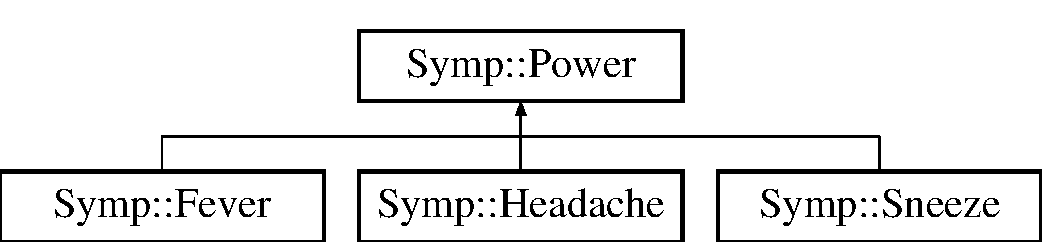
\includegraphics[height=2.000000cm]{class_symp_1_1_power}
\end{center}
\end{figure}
\subsection*{Public Member Functions}
\begin{DoxyCompactItemize}
\item 
\hyperlink{class_symp_1_1_power_a5848fe6b14bb7df471bd4b09a0a1f51d}{Power} ()
\begin{DoxyCompactList}\small\item\em \hyperlink{class_symp_1_1_power}{Power} class constructor. \end{DoxyCompactList}\item 
virtual \hyperlink{class_symp_1_1_power_ae20f1c2cba6616ed2903a8f082a0098f}{$\sim$\-Power} ()
\begin{DoxyCompactList}\small\item\em \hyperlink{class_symp_1_1_power}{Power} class destructor. \end{DoxyCompactList}\item 
virtual void \hyperlink{class_symp_1_1_power_a148a017c9f01bea343d062460074eae5}{execute} ()
\begin{DoxyCompactList}\small\item\em Virtual method This method can be implemented by the inherited class \#\-Sneeze, \#\-Fever and \#\-Headache. \end{DoxyCompactList}\item 
virtual void \hyperlink{class_symp_1_1_power_acc825d941b947be435944fc4d876a118}{force\-Execution} ()
\begin{DoxyCompactList}\small\item\em Virtual method This method can be implemented by the inherited class \#\-Sneeze, \#\-Fever and \#\-Headache. \end{DoxyCompactList}\item 
bool \hyperlink{class_symp_1_1_power_af57b06001854e1fe33589af20be33ce0}{is\-Activated} () const 
\begin{DoxyCompactList}\small\item\em Get the state of the current power. Warning \-: some powers have subtilities (example of the \hyperlink{class_symp_1_1_sneeze}{Sneeze}, with the warning and the real sneeze, both when the power is activated). \end{DoxyCompactList}\end{DoxyCompactItemize}
\subsection*{Protected Member Functions}
\begin{DoxyCompactItemize}
\item 
void \hyperlink{class_symp_1_1_power_a754fa6ce4b830bd75e8a3402df4d4b15}{activate} ()
\begin{DoxyCompactList}\small\item\em Activate the current power. \end{DoxyCompactList}\item 
void \hyperlink{class_symp_1_1_power_a27f953cf5f790649fba090ed2ba1af3d}{deactivate} ()
\begin{DoxyCompactList}\small\item\em Deactivate the current power. \end{DoxyCompactList}\end{DoxyCompactItemize}
\subsection*{Protected Attributes}
\begin{DoxyCompactItemize}
\item 
I\-N\-D\-\_\-\-Timer $\ast$ \hyperlink{class_symp_1_1_power_a8f421a13e9e62dac404c6c1ef4862045}{m\-\_\-p\-Timer}
\end{DoxyCompactItemize}


\subsection{Detailed Description}
is an abstract class with a pure virtual method named \hyperlink{class_symp_1_1_power_a148a017c9f01bea343d062460074eae5}{execute()}. There are three powers inherited from this class \-: \#\-Sneeze, \#\-Fever and \#\-Headache. Each one of them has to implement the virtual \hyperlink{class_symp_1_1_power_a148a017c9f01bea343d062460074eae5}{execute()} method. \begin{DoxySeeAlso}{See Also}
\hyperlink{class_symp_1_1_sneeze}{Sneeze} 

\hyperlink{class_symp_1_1_fever}{Fever} 

\hyperlink{class_symp_1_1_headache}{Headache} 
\end{DoxySeeAlso}


Definition at line 37 of file Power.\-h.



\subsection{Constructor \& Destructor Documentation}
\hypertarget{class_symp_1_1_power_a5848fe6b14bb7df471bd4b09a0a1f51d}{\index{Symp\-::\-Power@{Symp\-::\-Power}!Power@{Power}}
\index{Power@{Power}!Symp::Power@{Symp\-::\-Power}}
\subsubsection[{Power}]{\setlength{\rightskip}{0pt plus 5cm}Symp\-::\-Power\-::\-Power (
\begin{DoxyParamCaption}
{}
\end{DoxyParamCaption}
)\hspace{0.3cm}{\ttfamily [inline]}}}\label{class_symp_1_1_power_a5848fe6b14bb7df471bd4b09a0a1f51d}


\hyperlink{class_symp_1_1_power}{Power} class constructor. 



Definition at line 44 of file Power.\-h.

\hypertarget{class_symp_1_1_power_ae20f1c2cba6616ed2903a8f082a0098f}{\index{Symp\-::\-Power@{Symp\-::\-Power}!$\sim$\-Power@{$\sim$\-Power}}
\index{$\sim$\-Power@{$\sim$\-Power}!Symp::Power@{Symp\-::\-Power}}
\subsubsection[{$\sim$\-Power}]{\setlength{\rightskip}{0pt plus 5cm}virtual Symp\-::\-Power\-::$\sim$\-Power (
\begin{DoxyParamCaption}
{}
\end{DoxyParamCaption}
)\hspace{0.3cm}{\ttfamily [inline]}, {\ttfamily [virtual]}}}\label{class_symp_1_1_power_ae20f1c2cba6616ed2903a8f082a0098f}


\hyperlink{class_symp_1_1_power}{Power} class destructor. 



Definition at line 52 of file Power.\-h.



\subsection{Member Function Documentation}
\hypertarget{class_symp_1_1_power_a754fa6ce4b830bd75e8a3402df4d4b15}{\index{Symp\-::\-Power@{Symp\-::\-Power}!activate@{activate}}
\index{activate@{activate}!Symp::Power@{Symp\-::\-Power}}
\subsubsection[{activate}]{\setlength{\rightskip}{0pt plus 5cm}void Symp\-::\-Power\-::activate (
\begin{DoxyParamCaption}
{}
\end{DoxyParamCaption}
)\hspace{0.3cm}{\ttfamily [inline]}, {\ttfamily [protected]}}}\label{class_symp_1_1_power_a754fa6ce4b830bd75e8a3402df4d4b15}


Activate the current power. 



Definition at line 78 of file Power.\-h.

\hypertarget{class_symp_1_1_power_a27f953cf5f790649fba090ed2ba1af3d}{\index{Symp\-::\-Power@{Symp\-::\-Power}!deactivate@{deactivate}}
\index{deactivate@{deactivate}!Symp::Power@{Symp\-::\-Power}}
\subsubsection[{deactivate}]{\setlength{\rightskip}{0pt plus 5cm}void Symp\-::\-Power\-::deactivate (
\begin{DoxyParamCaption}
{}
\end{DoxyParamCaption}
)\hspace{0.3cm}{\ttfamily [inline]}, {\ttfamily [protected]}}}\label{class_symp_1_1_power_a27f953cf5f790649fba090ed2ba1af3d}


Deactivate the current power. 



Definition at line 85 of file Power.\-h.

\hypertarget{class_symp_1_1_power_a148a017c9f01bea343d062460074eae5}{\index{Symp\-::\-Power@{Symp\-::\-Power}!execute@{execute}}
\index{execute@{execute}!Symp::Power@{Symp\-::\-Power}}
\subsubsection[{execute}]{\setlength{\rightskip}{0pt plus 5cm}virtual void Symp\-::\-Power\-::execute (
\begin{DoxyParamCaption}
{}
\end{DoxyParamCaption}
)\hspace{0.3cm}{\ttfamily [inline]}, {\ttfamily [virtual]}}}\label{class_symp_1_1_power_a148a017c9f01bea343d062460074eae5}


Virtual method This method can be implemented by the inherited class \#\-Sneeze, \#\-Fever and \#\-Headache. 



Reimplemented in \hyperlink{class_symp_1_1_headache_a5de12b8de4529142a63e738132292e83}{Symp\-::\-Headache}, \hyperlink{class_symp_1_1_sneeze_aaaf79da47ab1a8888f4af276e31087f1}{Symp\-::\-Sneeze}, and \hyperlink{class_symp_1_1_fever_a963f59082a92165475663d3c359ffbf2}{Symp\-::\-Fever}.



Definition at line 58 of file Power.\-h.

\hypertarget{class_symp_1_1_power_acc825d941b947be435944fc4d876a118}{\index{Symp\-::\-Power@{Symp\-::\-Power}!force\-Execution@{force\-Execution}}
\index{force\-Execution@{force\-Execution}!Symp::Power@{Symp\-::\-Power}}
\subsubsection[{force\-Execution}]{\setlength{\rightskip}{0pt plus 5cm}virtual void Symp\-::\-Power\-::force\-Execution (
\begin{DoxyParamCaption}
{}
\end{DoxyParamCaption}
)\hspace{0.3cm}{\ttfamily [inline]}, {\ttfamily [virtual]}}}\label{class_symp_1_1_power_acc825d941b947be435944fc4d876a118}


Virtual method This method can be implemented by the inherited class \#\-Sneeze, \#\-Fever and \#\-Headache. 



Reimplemented in \hyperlink{class_symp_1_1_headache_adfb5b616e538d1c62062b854cdae464d}{Symp\-::\-Headache}, \hyperlink{class_symp_1_1_sneeze_a76aec7dca3104e9e0b8c2dade0d9eac9}{Symp\-::\-Sneeze}, and \hyperlink{class_symp_1_1_fever_a7dcf044b45ffc3f6ce6096ac9112d6d9}{Symp\-::\-Fever}.



Definition at line 65 of file Power.\-h.

\hypertarget{class_symp_1_1_power_af57b06001854e1fe33589af20be33ce0}{\index{Symp\-::\-Power@{Symp\-::\-Power}!is\-Activated@{is\-Activated}}
\index{is\-Activated@{is\-Activated}!Symp::Power@{Symp\-::\-Power}}
\subsubsection[{is\-Activated}]{\setlength{\rightskip}{0pt plus 5cm}bool Symp\-::\-Power\-::is\-Activated (
\begin{DoxyParamCaption}
{}
\end{DoxyParamCaption}
) const\hspace{0.3cm}{\ttfamily [inline]}}}\label{class_symp_1_1_power_af57b06001854e1fe33589af20be33ce0}


Get the state of the current power. Warning \-: some powers have subtilities (example of the \hyperlink{class_symp_1_1_sneeze}{Sneeze}, with the warning and the real sneeze, both when the power is activated). 



Definition at line 71 of file Power.\-h.



\subsection{Member Data Documentation}
\hypertarget{class_symp_1_1_power_a8f421a13e9e62dac404c6c1ef4862045}{\index{Symp\-::\-Power@{Symp\-::\-Power}!m\-\_\-p\-Timer@{m\-\_\-p\-Timer}}
\index{m\-\_\-p\-Timer@{m\-\_\-p\-Timer}!Symp::Power@{Symp\-::\-Power}}
\subsubsection[{m\-\_\-p\-Timer}]{\setlength{\rightskip}{0pt plus 5cm}I\-N\-D\-\_\-\-Timer$\ast$ Symp\-::\-Power\-::m\-\_\-p\-Timer\hspace{0.3cm}{\ttfamily [protected]}}}\label{class_symp_1_1_power_a8f421a13e9e62dac404c6c1ef4862045}
This timer is used to know if the animation is playing 

Definition at line 89 of file Power.\-h.



The documentation for this class was generated from the following file\-:\begin{DoxyCompactItemize}
\item 
/home/cecilia/\-Documents/\-Symptogen/src/power/\hyperlink{_power_8h}{Power.\-h}\end{DoxyCompactItemize}

\hypertarget{class_symp_1_1_render}{\section{Symp\-:\-:Render Class Reference}
\label{class_symp_1_1_render}\index{Symp\-::\-Render@{Symp\-::\-Render}}
}


{\ttfamily \#include $<$Render.\-h$>$}

\subsection*{Public Member Functions}
\begin{DoxyCompactItemize}
\item 
\hyperlink{class_symp_1_1_render_a4505792fcfee84c6c94b87f3f5779891}{Render} ()
\item 
I\-N\-D\-\_\-\-Window $\ast$ \hyperlink{class_symp_1_1_render_a9b258118ee8e8dafb6668de699ee0402}{init} (const char $\ast$title, int width, int height, int bpp, bool vsync, bool fs, bool d\-Buffer)
\item 
\hyperlink{class_symp_1_1_render_a86c29b1e0beccbc1a7c83717dac38a44}{$\sim$\-Render} ()
\item 
void \hyperlink{class_symp_1_1_render_aa94659e2d71c3fccfde9f5fdd9bbfe29}{begin\-Scene} ()
\item 
void \hyperlink{class_symp_1_1_render_a750acc68c58537a7f6d73ba750719713}{end\-Scene} ()
\item 
void \hyperlink{class_symp_1_1_render_a96aff84eb780881d2a389d3f13841955}{clear\-View\-Port} (unsigned char p\-R, unsigned char p\-G, unsigned char p\-B)
\item 
I\-N\-D\-\_\-\-Render $\ast$ \hyperlink{class_symp_1_1_render_a393d266b34a1fcf4ef2912d9d7658147}{get\-I\-N\-D\-\_\-\-Render} () const 
\item 
float \hyperlink{class_symp_1_1_render_a6a0ecd56872f64dfa2417a9194c75f1f}{get\-Zoom} () const 
\item 
bool \hyperlink{class_symp_1_1_render_aa08df7e32f8115a4ec5e616a60a6615e}{is\-Full\-Screen} () const 
\item 
float \hyperlink{class_symp_1_1_render_a572084595ab2928bd5ed456ee3ffffea}{get\-Camera\-Angle} () const 
\item 
void \hyperlink{class_symp_1_1_render_aac4ba9ac09f2478851c7859744af121d}{set\-Camera\-Position} (float pos\-X, float pos\-Y)
\item 
void \hyperlink{class_symp_1_1_render_a8f5b9ca7ff4d32efbc933bcc8cadbc55}{set\-Zoom} (float zoom)
\item 
void \hyperlink{class_symp_1_1_render_a9e51c417fc122dd82f2be670f85373c9}{set\-Camera\-Angle} (float angle)
\item 
void \hyperlink{class_symp_1_1_render_ae134663e4d5709af44c76252d2abceed}{reset\-Camera} (float dino\-Pos\-X, float dino\-Pos\-Y)
\item 
void \hyperlink{class_symp_1_1_render_a8a4aed45f564547272e009aa53b10927}{set\-Camera} ()
\item 
void \hyperlink{class_symp_1_1_render_a9545ec8794a0b04ab3a1cc38c1b22d92}{toggle\-Full\-Screen} ()
\end{DoxyCompactItemize}


\subsection{Detailed Description}
Facade of I\-N\-D\-\_\-\-Render. 

Definition at line 14 of file Render.\-h.



\subsection{Constructor \& Destructor Documentation}
\hypertarget{class_symp_1_1_render_a4505792fcfee84c6c94b87f3f5779891}{\index{Symp\-::\-Render@{Symp\-::\-Render}!Render@{Render}}
\index{Render@{Render}!Symp::Render@{Symp\-::\-Render}}
\subsubsection[{Render}]{\setlength{\rightskip}{0pt plus 5cm}Symp\-::\-Render\-::\-Render (
\begin{DoxyParamCaption}
{}
\end{DoxyParamCaption}
)}}\label{class_symp_1_1_render_a4505792fcfee84c6c94b87f3f5779891}


Definition at line 5 of file Render.\-cpp.

\hypertarget{class_symp_1_1_render_a86c29b1e0beccbc1a7c83717dac38a44}{\index{Symp\-::\-Render@{Symp\-::\-Render}!$\sim$\-Render@{$\sim$\-Render}}
\index{$\sim$\-Render@{$\sim$\-Render}!Symp::Render@{Symp\-::\-Render}}
\subsubsection[{$\sim$\-Render}]{\setlength{\rightskip}{0pt plus 5cm}Symp\-::\-Render\-::$\sim$\-Render (
\begin{DoxyParamCaption}
{}
\end{DoxyParamCaption}
)}}\label{class_symp_1_1_render_a86c29b1e0beccbc1a7c83717dac38a44}


Definition at line 16 of file Render.\-cpp.



\subsection{Member Function Documentation}
\hypertarget{class_symp_1_1_render_aa94659e2d71c3fccfde9f5fdd9bbfe29}{\index{Symp\-::\-Render@{Symp\-::\-Render}!begin\-Scene@{begin\-Scene}}
\index{begin\-Scene@{begin\-Scene}!Symp::Render@{Symp\-::\-Render}}
\subsubsection[{begin\-Scene}]{\setlength{\rightskip}{0pt plus 5cm}void Symp\-::\-Render\-::begin\-Scene (
\begin{DoxyParamCaption}
{}
\end{DoxyParamCaption}
)}}\label{class_symp_1_1_render_aa94659e2d71c3fccfde9f5fdd9bbfe29}


Definition at line 22 of file Render.\-cpp.

\hypertarget{class_symp_1_1_render_a96aff84eb780881d2a389d3f13841955}{\index{Symp\-::\-Render@{Symp\-::\-Render}!clear\-View\-Port@{clear\-View\-Port}}
\index{clear\-View\-Port@{clear\-View\-Port}!Symp::Render@{Symp\-::\-Render}}
\subsubsection[{clear\-View\-Port}]{\setlength{\rightskip}{0pt plus 5cm}void Symp\-::\-Render\-::clear\-View\-Port (
\begin{DoxyParamCaption}
\item[{unsigned char}]{p\-R, }
\item[{unsigned char}]{p\-G, }
\item[{unsigned char}]{p\-B}
\end{DoxyParamCaption}
)}}\label{class_symp_1_1_render_a96aff84eb780881d2a389d3f13841955}


Definition at line 30 of file Render.\-cpp.

\hypertarget{class_symp_1_1_render_a750acc68c58537a7f6d73ba750719713}{\index{Symp\-::\-Render@{Symp\-::\-Render}!end\-Scene@{end\-Scene}}
\index{end\-Scene@{end\-Scene}!Symp::Render@{Symp\-::\-Render}}
\subsubsection[{end\-Scene}]{\setlength{\rightskip}{0pt plus 5cm}void Symp\-::\-Render\-::end\-Scene (
\begin{DoxyParamCaption}
{}
\end{DoxyParamCaption}
)}}\label{class_symp_1_1_render_a750acc68c58537a7f6d73ba750719713}


Definition at line 26 of file Render.\-cpp.

\hypertarget{class_symp_1_1_render_a572084595ab2928bd5ed456ee3ffffea}{\index{Symp\-::\-Render@{Symp\-::\-Render}!get\-Camera\-Angle@{get\-Camera\-Angle}}
\index{get\-Camera\-Angle@{get\-Camera\-Angle}!Symp::Render@{Symp\-::\-Render}}
\subsubsection[{get\-Camera\-Angle}]{\setlength{\rightskip}{0pt plus 5cm}float Symp\-::\-Render\-::get\-Camera\-Angle (
\begin{DoxyParamCaption}
{}
\end{DoxyParamCaption}
) const\hspace{0.3cm}{\ttfamily [inline]}}}\label{class_symp_1_1_render_a572084595ab2928bd5ed456ee3ffffea}


Definition at line 31 of file Render.\-h.

\hypertarget{class_symp_1_1_render_a393d266b34a1fcf4ef2912d9d7658147}{\index{Symp\-::\-Render@{Symp\-::\-Render}!get\-I\-N\-D\-\_\-\-Render@{get\-I\-N\-D\-\_\-\-Render}}
\index{get\-I\-N\-D\-\_\-\-Render@{get\-I\-N\-D\-\_\-\-Render}!Symp::Render@{Symp\-::\-Render}}
\subsubsection[{get\-I\-N\-D\-\_\-\-Render}]{\setlength{\rightskip}{0pt plus 5cm}I\-N\-D\-\_\-\-Render$\ast$ Symp\-::\-Render\-::get\-I\-N\-D\-\_\-\-Render (
\begin{DoxyParamCaption}
{}
\end{DoxyParamCaption}
) const\hspace{0.3cm}{\ttfamily [inline]}}}\label{class_symp_1_1_render_a393d266b34a1fcf4ef2912d9d7658147}


Definition at line 28 of file Render.\-h.

\hypertarget{class_symp_1_1_render_a6a0ecd56872f64dfa2417a9194c75f1f}{\index{Symp\-::\-Render@{Symp\-::\-Render}!get\-Zoom@{get\-Zoom}}
\index{get\-Zoom@{get\-Zoom}!Symp::Render@{Symp\-::\-Render}}
\subsubsection[{get\-Zoom}]{\setlength{\rightskip}{0pt plus 5cm}float Symp\-::\-Render\-::get\-Zoom (
\begin{DoxyParamCaption}
{}
\end{DoxyParamCaption}
) const\hspace{0.3cm}{\ttfamily [inline]}}}\label{class_symp_1_1_render_a6a0ecd56872f64dfa2417a9194c75f1f}


Definition at line 29 of file Render.\-h.

\hypertarget{class_symp_1_1_render_a9b258118ee8e8dafb6668de699ee0402}{\index{Symp\-::\-Render@{Symp\-::\-Render}!init@{init}}
\index{init@{init}!Symp::Render@{Symp\-::\-Render}}
\subsubsection[{init}]{\setlength{\rightskip}{0pt plus 5cm}I\-N\-D\-\_\-\-Window $\ast$ Symp\-::\-Render\-::init (
\begin{DoxyParamCaption}
\item[{const char $\ast$}]{title, }
\item[{int}]{width, }
\item[{int}]{height, }
\item[{int}]{bpp, }
\item[{bool}]{vsync, }
\item[{bool}]{fs, }
\item[{bool}]{d\-Buffer}
\end{DoxyParamCaption}
)}}\label{class_symp_1_1_render_a9b258118ee8e8dafb6668de699ee0402}


Definition at line 11 of file Render.\-cpp.

\hypertarget{class_symp_1_1_render_aa08df7e32f8115a4ec5e616a60a6615e}{\index{Symp\-::\-Render@{Symp\-::\-Render}!is\-Full\-Screen@{is\-Full\-Screen}}
\index{is\-Full\-Screen@{is\-Full\-Screen}!Symp::Render@{Symp\-::\-Render}}
\subsubsection[{is\-Full\-Screen}]{\setlength{\rightskip}{0pt plus 5cm}bool Symp\-::\-Render\-::is\-Full\-Screen (
\begin{DoxyParamCaption}
{}
\end{DoxyParamCaption}
) const\hspace{0.3cm}{\ttfamily [inline]}}}\label{class_symp_1_1_render_aa08df7e32f8115a4ec5e616a60a6615e}


Definition at line 30 of file Render.\-h.

\hypertarget{class_symp_1_1_render_ae134663e4d5709af44c76252d2abceed}{\index{Symp\-::\-Render@{Symp\-::\-Render}!reset\-Camera@{reset\-Camera}}
\index{reset\-Camera@{reset\-Camera}!Symp::Render@{Symp\-::\-Render}}
\subsubsection[{reset\-Camera}]{\setlength{\rightskip}{0pt plus 5cm}void Symp\-::\-Render\-::reset\-Camera (
\begin{DoxyParamCaption}
\item[{float}]{dino\-Pos\-X, }
\item[{float}]{dino\-Pos\-Y}
\end{DoxyParamCaption}
)}}\label{class_symp_1_1_render_ae134663e4d5709af44c76252d2abceed}


Definition at line 50 of file Render.\-cpp.

\hypertarget{class_symp_1_1_render_a8a4aed45f564547272e009aa53b10927}{\index{Symp\-::\-Render@{Symp\-::\-Render}!set\-Camera@{set\-Camera}}
\index{set\-Camera@{set\-Camera}!Symp::Render@{Symp\-::\-Render}}
\subsubsection[{set\-Camera}]{\setlength{\rightskip}{0pt plus 5cm}void Symp\-::\-Render\-::set\-Camera (
\begin{DoxyParamCaption}
{}
\end{DoxyParamCaption}
)}}\label{class_symp_1_1_render_a8a4aed45f564547272e009aa53b10927}


Definition at line 42 of file Render.\-cpp.

\hypertarget{class_symp_1_1_render_a9e51c417fc122dd82f2be670f85373c9}{\index{Symp\-::\-Render@{Symp\-::\-Render}!set\-Camera\-Angle@{set\-Camera\-Angle}}
\index{set\-Camera\-Angle@{set\-Camera\-Angle}!Symp::Render@{Symp\-::\-Render}}
\subsubsection[{set\-Camera\-Angle}]{\setlength{\rightskip}{0pt plus 5cm}void Symp\-::\-Render\-::set\-Camera\-Angle (
\begin{DoxyParamCaption}
\item[{float}]{angle}
\end{DoxyParamCaption}
)}}\label{class_symp_1_1_render_a9e51c417fc122dd82f2be670f85373c9}


Definition at line 46 of file Render.\-cpp.

\hypertarget{class_symp_1_1_render_aac4ba9ac09f2478851c7859744af121d}{\index{Symp\-::\-Render@{Symp\-::\-Render}!set\-Camera\-Position@{set\-Camera\-Position}}
\index{set\-Camera\-Position@{set\-Camera\-Position}!Symp::Render@{Symp\-::\-Render}}
\subsubsection[{set\-Camera\-Position}]{\setlength{\rightskip}{0pt plus 5cm}void Symp\-::\-Render\-::set\-Camera\-Position (
\begin{DoxyParamCaption}
\item[{float}]{pos\-X, }
\item[{float}]{pos\-Y}
\end{DoxyParamCaption}
)}}\label{class_symp_1_1_render_aac4ba9ac09f2478851c7859744af121d}


Definition at line 34 of file Render.\-cpp.

\hypertarget{class_symp_1_1_render_a8f5b9ca7ff4d32efbc933bcc8cadbc55}{\index{Symp\-::\-Render@{Symp\-::\-Render}!set\-Zoom@{set\-Zoom}}
\index{set\-Zoom@{set\-Zoom}!Symp::Render@{Symp\-::\-Render}}
\subsubsection[{set\-Zoom}]{\setlength{\rightskip}{0pt plus 5cm}void Symp\-::\-Render\-::set\-Zoom (
\begin{DoxyParamCaption}
\item[{float}]{zoom}
\end{DoxyParamCaption}
)}}\label{class_symp_1_1_render_a8f5b9ca7ff4d32efbc933bcc8cadbc55}


Definition at line 38 of file Render.\-cpp.

\hypertarget{class_symp_1_1_render_a9545ec8794a0b04ab3a1cc38c1b22d92}{\index{Symp\-::\-Render@{Symp\-::\-Render}!toggle\-Full\-Screen@{toggle\-Full\-Screen}}
\index{toggle\-Full\-Screen@{toggle\-Full\-Screen}!Symp::Render@{Symp\-::\-Render}}
\subsubsection[{toggle\-Full\-Screen}]{\setlength{\rightskip}{0pt plus 5cm}void Symp\-::\-Render\-::toggle\-Full\-Screen (
\begin{DoxyParamCaption}
{}
\end{DoxyParamCaption}
)}}\label{class_symp_1_1_render_a9545ec8794a0b04ab3a1cc38c1b22d92}


Definition at line 54 of file Render.\-cpp.



The documentation for this class was generated from the following files\-:\begin{DoxyCompactItemize}
\item 
/home/cecilia/\-Documents/\-Symptogen/src/render/\hyperlink{_render_8h}{Render.\-h}\item 
/home/cecilia/\-Documents/\-Symptogen/src/render/\hyperlink{_render_8cpp}{Render.\-cpp}\end{DoxyCompactItemize}

\hypertarget{class_symp_1_1_render_entity}{\section{Symp\-:\-:Render\-Entity Class Reference}
\label{class_symp_1_1_render_entity}\index{Symp\-::\-Render\-Entity@{Symp\-::\-Render\-Entity}}
}


{\ttfamily \#include $<$Render\-Entity.\-h$>$}

\subsection*{Public Member Functions}
\begin{DoxyCompactItemize}
\item 
\hyperlink{class_symp_1_1_render_entity_ae2fe86c9be1225441978cc61a1fa8d15}{Render\-Entity} (const char $\ast$file\-Path, \hyperlink{namespace_symp_a1f2e90bddea116ff8d3e9e9b7cd34f37}{Render\-Type} render\-Type)
\begin{DoxyCompactList}\small\item\em Create the render entity. Create a render entity means creating an I\-N\-D\-\_\-\-Entity2d, set a surface or an animtion to it (depend on the render\-Type parameter), add the surface or the animation to the right manager (I\-N\-D\-\_\-\-Surface\-Manager, or I\-N\-D\-\_\-\-Animation\-Manager). Warning \-: this function closes the application if the file\-Path is wrong. \end{DoxyCompactList}\item 
\hyperlink{class_symp_1_1_render_entity_a3fa4ec2a1316e8c20e13021cd8c606d7}{Render\-Entity} ()
\begin{DoxyCompactList}\small\item\em Create the render entity. Create a render entity without defined texture. The aim is to use the Indielib primitives like I\-N\-D\-\_\-\-R\-E\-G\-U\-L\-A\-R\-A\-\_\-\-P\-O\-L\-Y which does not need a texture. \end{DoxyCompactList}\item 
\hyperlink{class_symp_1_1_render_entity_ae452869a384352c13c60db26d1dbc823}{$\sim$\-Render\-Entity} ()
\begin{DoxyCompactList}\small\item\em Delete the render entity. \end{DoxyCompactList}\item 
I\-N\-D\-\_\-\-Entity2d $\ast$ \hyperlink{class_symp_1_1_render_entity_a6adf4a950ce264f59bf3fbbc085aa280}{get\-I\-N\-D\-\_\-\-Entity2d} () const 
\item 
I\-N\-D\-\_\-\-Surface $\ast$ \hyperlink{class_symp_1_1_render_entity_a22980c9774e7e2f9b7664b994a07d98a}{get\-Surface} () const 
\item 
I\-N\-D\-\_\-\-Animation $\ast$ \hyperlink{class_symp_1_1_render_entity_a4aa566eb8d7722b7b655d4b49a54cc68}{get\-Animation} () const 
\item 
unsigned int \hyperlink{class_symp_1_1_render_entity_a352c69cb6974d124ad066d0b7b6c4981}{get\-Sequence} () const 
\item 
bool \hyperlink{class_symp_1_1_render_entity_a7d3eb409d809bf25ee79de81374fbda6}{is\-Show} () const 
\item 
int \hyperlink{class_symp_1_1_render_entity_ae2a81c03c6fffd2ba17ed68e9ed800f1}{get\-Opacity} () const 
\item 
float \hyperlink{class_symp_1_1_render_entity_a9665208c56b63e4c294e099e52a1f93e}{get\-Pos\-X} () const 
\item 
float \hyperlink{class_symp_1_1_render_entity_a379b1ea5104113cba5a1a561fa06570c}{get\-Pos\-Y} () const 
\item 
int \hyperlink{class_symp_1_1_render_entity_a179b72bcc0919c753b76c32c2b9f16af}{get\-Width} () const 
\item 
int \hyperlink{class_symp_1_1_render_entity_a427e9541ade5428f90794eb7380ab761}{get\-Height} () const 
\item 
bool \hyperlink{class_symp_1_1_render_entity_a48ab463295cf1edc65fcf06e46928ba4}{is\-Animation\-Playing} () const 
\item 
bool \hyperlink{class_symp_1_1_render_entity_a58303e3e44a9a4fcf49cb8ba86e684ba}{is\-Animation\-Finish} () const 
\item 
bool \hyperlink{class_symp_1_1_render_entity_abf68a93294e3bf55e298088e829eaf74}{is\-Flipped\-Horizontaly} () const 
\item 
bool \hyperlink{class_symp_1_1_render_entity_ab3677488f3ebdf686b3e7f44db081798}{is\-Flipped\-Verticaly} () const 
\item 
void \hyperlink{class_symp_1_1_render_entity_a5d12b22c3e790569bf98918a7aae91f3}{set\-Surface} (const char $\ast$file\-Path)
\item 
void \hyperlink{class_symp_1_1_render_entity_ac47597dd2ebf97b78ea7696a0e54903f}{set\-Animation} (const char $\ast$file\-Path)
\item 
void \hyperlink{class_symp_1_1_render_entity_a33cf06dfd78275fb847c837ccf4a04a0}{set\-Sequence} (unsigned int p\-Sequence)
\item 
void \hyperlink{class_symp_1_1_render_entity_ab6deaa2a7c38603f08d2a5f3117d11a3}{set\-Num\-Replays} (int p\-Num\-Replays)
\item 
void \hyperlink{class_symp_1_1_render_entity_a19ce976bffb402245daba860b7b883c2}{set\-Show} (bool flag)
\item 
void \hyperlink{class_symp_1_1_render_entity_aaab48e2f1a0ffe21c3f9d41140d83b4d}{set\-Position} (float p\-X, float p\-Y)
\item 
void \hyperlink{class_symp_1_1_render_entity_af1921c608cf05ae595a0a1667c0e594b}{set\-Scale} (float p\-Sx, float p\-Sy)
\item 
void \hyperlink{class_symp_1_1_render_entity_a814a076e051dd35318b95b7079eb6259}{set\-Tint} (float r, float g, float b)
\item 
void \hyperlink{class_symp_1_1_render_entity_aa2033131f560efda6c1f7bd801a05721}{set\-Opacity} (int a)
\item 
void \hyperlink{class_symp_1_1_render_entity_a5f1f8c4c4691dd16f2f8f07c658b8e3c}{set\-Angle\-X\-Y\-Z} (float x, float y, float z)
\item 
void \hyperlink{class_symp_1_1_render_entity_a4a6b336b8a835788ae433b16e5944d53}{flip\-Horizontaly} (bool flip)
\item 
void \hyperlink{class_symp_1_1_render_entity_a390e02078053486a376fa28a1ad395aa}{flip\-Verticaly} (bool flip)
\item 
bool \hyperlink{class_symp_1_1_render_entity_a5cda1fcf2807cd5d488257ac97e6e537}{set\-Hot\-Spot} (float p\-X, float p\-Y)
\item 
void \hyperlink{class_symp_1_1_render_entity_a310ff71db866bc621f134b4fc49d55cc}{manage\-Animation\-Timer} (\hyperlink{namespace_symp_a0e94673adb6fed024bf03e95d9cfafba}{Animation\-Length} lenght=Animation\-Length\-::\-Other\-Length)
\end{DoxyCompactItemize}
\subsection*{Static Public Member Functions}
\begin{DoxyCompactItemize}
\item 
static void \hyperlink{class_symp_1_1_render_entity_a023d97c9a548d7172ca25eb454885f41}{init} (\hyperlink{class_symp_1_1_render}{Render} $\ast$p\-Render)
\begin{DoxyCompactList}\small\item\em Set the render environment, needed to create render entities. Initialize an I\-N\-D\-\_\-\-Image\-Manager, a I\-N\-D\-\_\-\-Surface\-Manager, and an I\-N\-D\-\_\-\-Animation\-Manager. \end{DoxyCompactList}\item 
static void \hyperlink{class_symp_1_1_render_entity_ae46c9cd64da0974544a24c718b87a7ed}{end} ()
\begin{DoxyCompactList}\small\item\em Deallocate the render environment. Deallocate the I\-N\-D\-\_\-\-Image\-Manager, the I\-N\-D\-\_\-\-Surface\-Manager, and the I\-N\-D\-\_\-\-Animation\-Manager. \end{DoxyCompactList}\end{DoxyCompactItemize}
\subsection*{Static Public Attributes}
\begin{DoxyCompactItemize}
\item 
static std\-::map$<$ std\-::string, \\*
I\-N\-D\-\_\-\-Surface $\ast$ $>$ \hyperlink{class_symp_1_1_render_entity_a98acc72744a48bef45dcf4b0a9b0e8f7}{s\-\_\-surface\-Map} = std\-::map$<$std\-::string, I\-N\-D\-\_\-\-Surface$\ast$$>$()
\item 
static std\-::map$<$ std\-::string, \\*
I\-N\-D\-\_\-\-Animation $\ast$ $>$ \hyperlink{class_symp_1_1_render_entity_a6d0e13d1ba5cd1eaad7820e774acc867}{s\-\_\-animation\-Map} = std\-::map$<$std\-::string, I\-N\-D\-\_\-\-Animation$\ast$$>$()
\end{DoxyCompactItemize}


\subsection{Detailed Description}
Facade of I\-N\-D\-\_\-\-Entity2d. This class corresponds to all our render elements, visible in the game. They are store in the array m\-\_\-render\-Entity\-Array, contains in the \hyperlink{class_symp_1_1_entity_manager}{Entity\-Manager}. Warning \-: in the menu, we use \hyperlink{class_symp_1_1_gui_component}{Gui\-Component} (an other class, and an other facade of I\-N\-D\-\_\-\-Entity2d). It provides tools to \-:
\begin{DoxyItemize}
\item Set a surface
\item Set an animation \begin{DoxySeeAlso}{See Also}
\hyperlink{class_symp_1_1_entity_manager}{Entity\-Manager} 
\end{DoxySeeAlso}

\end{DoxyItemize}

Definition at line 50 of file Render\-Entity.\-h.



\subsection{Constructor \& Destructor Documentation}
\hypertarget{class_symp_1_1_render_entity_ae2fe86c9be1225441978cc61a1fa8d15}{\index{Symp\-::\-Render\-Entity@{Symp\-::\-Render\-Entity}!Render\-Entity@{Render\-Entity}}
\index{Render\-Entity@{Render\-Entity}!Symp::RenderEntity@{Symp\-::\-Render\-Entity}}
\subsubsection[{Render\-Entity}]{\setlength{\rightskip}{0pt plus 5cm}Symp\-::\-Render\-Entity\-::\-Render\-Entity (
\begin{DoxyParamCaption}
\item[{const char $\ast$}]{file\-Path, }
\item[{{\bf Render\-Type}}]{render\-Type}
\end{DoxyParamCaption}
)}}\label{class_symp_1_1_render_entity_ae2fe86c9be1225441978cc61a1fa8d15}


Create the render entity. Create a render entity means creating an I\-N\-D\-\_\-\-Entity2d, set a surface or an animtion to it (depend on the render\-Type parameter), add the surface or the animation to the right manager (I\-N\-D\-\_\-\-Surface\-Manager, or I\-N\-D\-\_\-\-Animation\-Manager). Warning \-: this function closes the application if the file\-Path is wrong. 



Definition at line 15 of file Render\-Entity.\-cpp.

\hypertarget{class_symp_1_1_render_entity_a3fa4ec2a1316e8c20e13021cd8c606d7}{\index{Symp\-::\-Render\-Entity@{Symp\-::\-Render\-Entity}!Render\-Entity@{Render\-Entity}}
\index{Render\-Entity@{Render\-Entity}!Symp::RenderEntity@{Symp\-::\-Render\-Entity}}
\subsubsection[{Render\-Entity}]{\setlength{\rightskip}{0pt plus 5cm}Symp\-::\-Render\-Entity\-::\-Render\-Entity (
\begin{DoxyParamCaption}
{}
\end{DoxyParamCaption}
)}}\label{class_symp_1_1_render_entity_a3fa4ec2a1316e8c20e13021cd8c606d7}


Create the render entity. Create a render entity without defined texture. The aim is to use the Indielib primitives like I\-N\-D\-\_\-\-R\-E\-G\-U\-L\-A\-R\-A\-\_\-\-P\-O\-L\-Y which does not need a texture. 



Definition at line 26 of file Render\-Entity.\-cpp.

\hypertarget{class_symp_1_1_render_entity_ae452869a384352c13c60db26d1dbc823}{\index{Symp\-::\-Render\-Entity@{Symp\-::\-Render\-Entity}!$\sim$\-Render\-Entity@{$\sim$\-Render\-Entity}}
\index{$\sim$\-Render\-Entity@{$\sim$\-Render\-Entity}!Symp::RenderEntity@{Symp\-::\-Render\-Entity}}
\subsubsection[{$\sim$\-Render\-Entity}]{\setlength{\rightskip}{0pt plus 5cm}Symp\-::\-Render\-Entity\-::$\sim$\-Render\-Entity (
\begin{DoxyParamCaption}
{}
\end{DoxyParamCaption}
)}}\label{class_symp_1_1_render_entity_ae452869a384352c13c60db26d1dbc823}


Delete the render entity. 



Definition at line 33 of file Render\-Entity.\-cpp.



\subsection{Member Function Documentation}
\hypertarget{class_symp_1_1_render_entity_ae46c9cd64da0974544a24c718b87a7ed}{\index{Symp\-::\-Render\-Entity@{Symp\-::\-Render\-Entity}!end@{end}}
\index{end@{end}!Symp::RenderEntity@{Symp\-::\-Render\-Entity}}
\subsubsection[{end}]{\setlength{\rightskip}{0pt plus 5cm}void Symp\-::\-Render\-Entity\-::end (
\begin{DoxyParamCaption}
{}
\end{DoxyParamCaption}
)\hspace{0.3cm}{\ttfamily [static]}}}\label{class_symp_1_1_render_entity_ae46c9cd64da0974544a24c718b87a7ed}


Deallocate the render environment. Deallocate the I\-N\-D\-\_\-\-Image\-Manager, the I\-N\-D\-\_\-\-Surface\-Manager, and the I\-N\-D\-\_\-\-Animation\-Manager. 



Definition at line 48 of file Render\-Entity.\-cpp.

\hypertarget{class_symp_1_1_render_entity_a4a6b336b8a835788ae433b16e5944d53}{\index{Symp\-::\-Render\-Entity@{Symp\-::\-Render\-Entity}!flip\-Horizontaly@{flip\-Horizontaly}}
\index{flip\-Horizontaly@{flip\-Horizontaly}!Symp::RenderEntity@{Symp\-::\-Render\-Entity}}
\subsubsection[{flip\-Horizontaly}]{\setlength{\rightskip}{0pt plus 5cm}void Symp\-::\-Render\-Entity\-::flip\-Horizontaly (
\begin{DoxyParamCaption}
\item[{bool}]{flip}
\end{DoxyParamCaption}
)\hspace{0.3cm}{\ttfamily [inline]}}}\label{class_symp_1_1_render_entity_a4a6b336b8a835788ae433b16e5944d53}


Definition at line 141 of file Render\-Entity.\-h.

\hypertarget{class_symp_1_1_render_entity_a390e02078053486a376fa28a1ad395aa}{\index{Symp\-::\-Render\-Entity@{Symp\-::\-Render\-Entity}!flip\-Verticaly@{flip\-Verticaly}}
\index{flip\-Verticaly@{flip\-Verticaly}!Symp::RenderEntity@{Symp\-::\-Render\-Entity}}
\subsubsection[{flip\-Verticaly}]{\setlength{\rightskip}{0pt plus 5cm}void Symp\-::\-Render\-Entity\-::flip\-Verticaly (
\begin{DoxyParamCaption}
\item[{bool}]{flip}
\end{DoxyParamCaption}
)\hspace{0.3cm}{\ttfamily [inline]}}}\label{class_symp_1_1_render_entity_a390e02078053486a376fa28a1ad395aa}


Definition at line 142 of file Render\-Entity.\-h.

\hypertarget{class_symp_1_1_render_entity_a4aa566eb8d7722b7b655d4b49a54cc68}{\index{Symp\-::\-Render\-Entity@{Symp\-::\-Render\-Entity}!get\-Animation@{get\-Animation}}
\index{get\-Animation@{get\-Animation}!Symp::RenderEntity@{Symp\-::\-Render\-Entity}}
\subsubsection[{get\-Animation}]{\setlength{\rightskip}{0pt plus 5cm}I\-N\-D\-\_\-\-Animation$\ast$ Symp\-::\-Render\-Entity\-::get\-Animation (
\begin{DoxyParamCaption}
{}
\end{DoxyParamCaption}
) const\hspace{0.3cm}{\ttfamily [inline]}}}\label{class_symp_1_1_render_entity_a4aa566eb8d7722b7b655d4b49a54cc68}


Definition at line 90 of file Render\-Entity.\-h.

\hypertarget{class_symp_1_1_render_entity_a427e9541ade5428f90794eb7380ab761}{\index{Symp\-::\-Render\-Entity@{Symp\-::\-Render\-Entity}!get\-Height@{get\-Height}}
\index{get\-Height@{get\-Height}!Symp::RenderEntity@{Symp\-::\-Render\-Entity}}
\subsubsection[{get\-Height}]{\setlength{\rightskip}{0pt plus 5cm}int Symp\-::\-Render\-Entity\-::get\-Height (
\begin{DoxyParamCaption}
{}
\end{DoxyParamCaption}
) const}}\label{class_symp_1_1_render_entity_a427e9541ade5428f90794eb7380ab761}
Get the real size of the render entity (includes the scale factor). Warning \-: if the render entity is an animtion, return the height of sequence 0. 

Definition at line 69 of file Render\-Entity.\-cpp.

\hypertarget{class_symp_1_1_render_entity_a6adf4a950ce264f59bf3fbbc085aa280}{\index{Symp\-::\-Render\-Entity@{Symp\-::\-Render\-Entity}!get\-I\-N\-D\-\_\-\-Entity2d@{get\-I\-N\-D\-\_\-\-Entity2d}}
\index{get\-I\-N\-D\-\_\-\-Entity2d@{get\-I\-N\-D\-\_\-\-Entity2d}!Symp::RenderEntity@{Symp\-::\-Render\-Entity}}
\subsubsection[{get\-I\-N\-D\-\_\-\-Entity2d}]{\setlength{\rightskip}{0pt plus 5cm}I\-N\-D\-\_\-\-Entity2d$\ast$ Symp\-::\-Render\-Entity\-::get\-I\-N\-D\-\_\-\-Entity2d (
\begin{DoxyParamCaption}
{}
\end{DoxyParamCaption}
) const\hspace{0.3cm}{\ttfamily [inline]}}}\label{class_symp_1_1_render_entity_a6adf4a950ce264f59bf3fbbc085aa280}
Getters 

Definition at line 88 of file Render\-Entity.\-h.

\hypertarget{class_symp_1_1_render_entity_ae2a81c03c6fffd2ba17ed68e9ed800f1}{\index{Symp\-::\-Render\-Entity@{Symp\-::\-Render\-Entity}!get\-Opacity@{get\-Opacity}}
\index{get\-Opacity@{get\-Opacity}!Symp::RenderEntity@{Symp\-::\-Render\-Entity}}
\subsubsection[{get\-Opacity}]{\setlength{\rightskip}{0pt plus 5cm}int Symp\-::\-Render\-Entity\-::get\-Opacity (
\begin{DoxyParamCaption}
{}
\end{DoxyParamCaption}
) const\hspace{0.3cm}{\ttfamily [inline]}}}\label{class_symp_1_1_render_entity_ae2a81c03c6fffd2ba17ed68e9ed800f1}


Definition at line 93 of file Render\-Entity.\-h.

\hypertarget{class_symp_1_1_render_entity_a9665208c56b63e4c294e099e52a1f93e}{\index{Symp\-::\-Render\-Entity@{Symp\-::\-Render\-Entity}!get\-Pos\-X@{get\-Pos\-X}}
\index{get\-Pos\-X@{get\-Pos\-X}!Symp::RenderEntity@{Symp\-::\-Render\-Entity}}
\subsubsection[{get\-Pos\-X}]{\setlength{\rightskip}{0pt plus 5cm}float Symp\-::\-Render\-Entity\-::get\-Pos\-X (
\begin{DoxyParamCaption}
{}
\end{DoxyParamCaption}
) const\hspace{0.3cm}{\ttfamily [inline]}}}\label{class_symp_1_1_render_entity_a9665208c56b63e4c294e099e52a1f93e}
Get the center X of the render entity. 

Definition at line 99 of file Render\-Entity.\-h.

\hypertarget{class_symp_1_1_render_entity_a379b1ea5104113cba5a1a561fa06570c}{\index{Symp\-::\-Render\-Entity@{Symp\-::\-Render\-Entity}!get\-Pos\-Y@{get\-Pos\-Y}}
\index{get\-Pos\-Y@{get\-Pos\-Y}!Symp::RenderEntity@{Symp\-::\-Render\-Entity}}
\subsubsection[{get\-Pos\-Y}]{\setlength{\rightskip}{0pt plus 5cm}float Symp\-::\-Render\-Entity\-::get\-Pos\-Y (
\begin{DoxyParamCaption}
{}
\end{DoxyParamCaption}
) const\hspace{0.3cm}{\ttfamily [inline]}}}\label{class_symp_1_1_render_entity_a379b1ea5104113cba5a1a561fa06570c}
Get the center Y of the render entity. 

Definition at line 104 of file Render\-Entity.\-h.

\hypertarget{class_symp_1_1_render_entity_a352c69cb6974d124ad066d0b7b6c4981}{\index{Symp\-::\-Render\-Entity@{Symp\-::\-Render\-Entity}!get\-Sequence@{get\-Sequence}}
\index{get\-Sequence@{get\-Sequence}!Symp::RenderEntity@{Symp\-::\-Render\-Entity}}
\subsubsection[{get\-Sequence}]{\setlength{\rightskip}{0pt plus 5cm}unsigned int Symp\-::\-Render\-Entity\-::get\-Sequence (
\begin{DoxyParamCaption}
{}
\end{DoxyParamCaption}
) const\hspace{0.3cm}{\ttfamily [inline]}}}\label{class_symp_1_1_render_entity_a352c69cb6974d124ad066d0b7b6c4981}


Definition at line 91 of file Render\-Entity.\-h.

\hypertarget{class_symp_1_1_render_entity_a22980c9774e7e2f9b7664b994a07d98a}{\index{Symp\-::\-Render\-Entity@{Symp\-::\-Render\-Entity}!get\-Surface@{get\-Surface}}
\index{get\-Surface@{get\-Surface}!Symp::RenderEntity@{Symp\-::\-Render\-Entity}}
\subsubsection[{get\-Surface}]{\setlength{\rightskip}{0pt plus 5cm}I\-N\-D\-\_\-\-Surface$\ast$ Symp\-::\-Render\-Entity\-::get\-Surface (
\begin{DoxyParamCaption}
{}
\end{DoxyParamCaption}
) const\hspace{0.3cm}{\ttfamily [inline]}}}\label{class_symp_1_1_render_entity_a22980c9774e7e2f9b7664b994a07d98a}


Definition at line 89 of file Render\-Entity.\-h.

\hypertarget{class_symp_1_1_render_entity_a179b72bcc0919c753b76c32c2b9f16af}{\index{Symp\-::\-Render\-Entity@{Symp\-::\-Render\-Entity}!get\-Width@{get\-Width}}
\index{get\-Width@{get\-Width}!Symp::RenderEntity@{Symp\-::\-Render\-Entity}}
\subsubsection[{get\-Width}]{\setlength{\rightskip}{0pt plus 5cm}int Symp\-::\-Render\-Entity\-::get\-Width (
\begin{DoxyParamCaption}
{}
\end{DoxyParamCaption}
) const}}\label{class_symp_1_1_render_entity_a179b72bcc0919c753b76c32c2b9f16af}
Get the real size of the render entity (includes the scale factor). Warning \-: if the render entity is an animtion, return the width of sequence 0. 

Definition at line 60 of file Render\-Entity.\-cpp.

\hypertarget{class_symp_1_1_render_entity_a023d97c9a548d7172ca25eb454885f41}{\index{Symp\-::\-Render\-Entity@{Symp\-::\-Render\-Entity}!init@{init}}
\index{init@{init}!Symp::RenderEntity@{Symp\-::\-Render\-Entity}}
\subsubsection[{init}]{\setlength{\rightskip}{0pt plus 5cm}void Symp\-::\-Render\-Entity\-::init (
\begin{DoxyParamCaption}
\item[{{\bf Render} $\ast$}]{p\-Render}
\end{DoxyParamCaption}
)\hspace{0.3cm}{\ttfamily [static]}}}\label{class_symp_1_1_render_entity_a023d97c9a548d7172ca25eb454885f41}


Set the render environment, needed to create render entities. Initialize an I\-N\-D\-\_\-\-Image\-Manager, a I\-N\-D\-\_\-\-Surface\-Manager, and an I\-N\-D\-\_\-\-Animation\-Manager. 



Definition at line 38 of file Render\-Entity.\-cpp.

\hypertarget{class_symp_1_1_render_entity_a58303e3e44a9a4fcf49cb8ba86e684ba}{\index{Symp\-::\-Render\-Entity@{Symp\-::\-Render\-Entity}!is\-Animation\-Finish@{is\-Animation\-Finish}}
\index{is\-Animation\-Finish@{is\-Animation\-Finish}!Symp::RenderEntity@{Symp\-::\-Render\-Entity}}
\subsubsection[{is\-Animation\-Finish}]{\setlength{\rightskip}{0pt plus 5cm}bool Symp\-::\-Render\-Entity\-::is\-Animation\-Finish (
\begin{DoxyParamCaption}
{}
\end{DoxyParamCaption}
) const\hspace{0.3cm}{\ttfamily [inline]}}}\label{class_symp_1_1_render_entity_a58303e3e44a9a4fcf49cb8ba86e684ba}


Definition at line 119 of file Render\-Entity.\-h.

\hypertarget{class_symp_1_1_render_entity_a48ab463295cf1edc65fcf06e46928ba4}{\index{Symp\-::\-Render\-Entity@{Symp\-::\-Render\-Entity}!is\-Animation\-Playing@{is\-Animation\-Playing}}
\index{is\-Animation\-Playing@{is\-Animation\-Playing}!Symp::RenderEntity@{Symp\-::\-Render\-Entity}}
\subsubsection[{is\-Animation\-Playing}]{\setlength{\rightskip}{0pt plus 5cm}bool Symp\-::\-Render\-Entity\-::is\-Animation\-Playing (
\begin{DoxyParamCaption}
{}
\end{DoxyParamCaption}
) const\hspace{0.3cm}{\ttfamily [inline]}}}\label{class_symp_1_1_render_entity_a48ab463295cf1edc65fcf06e46928ba4}


Definition at line 118 of file Render\-Entity.\-h.

\hypertarget{class_symp_1_1_render_entity_abf68a93294e3bf55e298088e829eaf74}{\index{Symp\-::\-Render\-Entity@{Symp\-::\-Render\-Entity}!is\-Flipped\-Horizontaly@{is\-Flipped\-Horizontaly}}
\index{is\-Flipped\-Horizontaly@{is\-Flipped\-Horizontaly}!Symp::RenderEntity@{Symp\-::\-Render\-Entity}}
\subsubsection[{is\-Flipped\-Horizontaly}]{\setlength{\rightskip}{0pt plus 5cm}bool Symp\-::\-Render\-Entity\-::is\-Flipped\-Horizontaly (
\begin{DoxyParamCaption}
{}
\end{DoxyParamCaption}
) const\hspace{0.3cm}{\ttfamily [inline]}}}\label{class_symp_1_1_render_entity_abf68a93294e3bf55e298088e829eaf74}


Definition at line 120 of file Render\-Entity.\-h.

\hypertarget{class_symp_1_1_render_entity_ab3677488f3ebdf686b3e7f44db081798}{\index{Symp\-::\-Render\-Entity@{Symp\-::\-Render\-Entity}!is\-Flipped\-Verticaly@{is\-Flipped\-Verticaly}}
\index{is\-Flipped\-Verticaly@{is\-Flipped\-Verticaly}!Symp::RenderEntity@{Symp\-::\-Render\-Entity}}
\subsubsection[{is\-Flipped\-Verticaly}]{\setlength{\rightskip}{0pt plus 5cm}bool Symp\-::\-Render\-Entity\-::is\-Flipped\-Verticaly (
\begin{DoxyParamCaption}
{}
\end{DoxyParamCaption}
) const\hspace{0.3cm}{\ttfamily [inline]}}}\label{class_symp_1_1_render_entity_ab3677488f3ebdf686b3e7f44db081798}


Definition at line 121 of file Render\-Entity.\-h.

\hypertarget{class_symp_1_1_render_entity_a7d3eb409d809bf25ee79de81374fbda6}{\index{Symp\-::\-Render\-Entity@{Symp\-::\-Render\-Entity}!is\-Show@{is\-Show}}
\index{is\-Show@{is\-Show}!Symp::RenderEntity@{Symp\-::\-Render\-Entity}}
\subsubsection[{is\-Show}]{\setlength{\rightskip}{0pt plus 5cm}bool Symp\-::\-Render\-Entity\-::is\-Show (
\begin{DoxyParamCaption}
{}
\end{DoxyParamCaption}
) const\hspace{0.3cm}{\ttfamily [inline]}}}\label{class_symp_1_1_render_entity_a7d3eb409d809bf25ee79de81374fbda6}


Definition at line 92 of file Render\-Entity.\-h.

\hypertarget{class_symp_1_1_render_entity_a310ff71db866bc621f134b4fc49d55cc}{\index{Symp\-::\-Render\-Entity@{Symp\-::\-Render\-Entity}!manage\-Animation\-Timer@{manage\-Animation\-Timer}}
\index{manage\-Animation\-Timer@{manage\-Animation\-Timer}!Symp::RenderEntity@{Symp\-::\-Render\-Entity}}
\subsubsection[{manage\-Animation\-Timer}]{\setlength{\rightskip}{0pt plus 5cm}void Symp\-::\-Render\-Entity\-::manage\-Animation\-Timer (
\begin{DoxyParamCaption}
\item[{{\bf Animation\-Length}}]{lenght = {\ttfamily AnimationLength\-:\-:OtherLength}}
\end{DoxyParamCaption}
)}}\label{class_symp_1_1_render_entity_a310ff71db866bc621f134b4fc49d55cc}
Start a Timer, or stop it if the time since the begining of the timer is superior to the all time of the animation. This function is used many times with the render entity of the dead dino (to not immediatly restart the level after the dino's dead). 

Definition at line 128 of file Render\-Entity.\-cpp.

\hypertarget{class_symp_1_1_render_entity_a5f1f8c4c4691dd16f2f8f07c658b8e3c}{\index{Symp\-::\-Render\-Entity@{Symp\-::\-Render\-Entity}!set\-Angle\-X\-Y\-Z@{set\-Angle\-X\-Y\-Z}}
\index{set\-Angle\-X\-Y\-Z@{set\-Angle\-X\-Y\-Z}!Symp::RenderEntity@{Symp\-::\-Render\-Entity}}
\subsubsection[{set\-Angle\-X\-Y\-Z}]{\setlength{\rightskip}{0pt plus 5cm}void Symp\-::\-Render\-Entity\-::set\-Angle\-X\-Y\-Z (
\begin{DoxyParamCaption}
\item[{float}]{x, }
\item[{float}]{y, }
\item[{float}]{z}
\end{DoxyParamCaption}
)\hspace{0.3cm}{\ttfamily [inline]}}}\label{class_symp_1_1_render_entity_a5f1f8c4c4691dd16f2f8f07c658b8e3c}


Definition at line 140 of file Render\-Entity.\-h.

\hypertarget{class_symp_1_1_render_entity_ac47597dd2ebf97b78ea7696a0e54903f}{\index{Symp\-::\-Render\-Entity@{Symp\-::\-Render\-Entity}!set\-Animation@{set\-Animation}}
\index{set\-Animation@{set\-Animation}!Symp::RenderEntity@{Symp\-::\-Render\-Entity}}
\subsubsection[{set\-Animation}]{\setlength{\rightskip}{0pt plus 5cm}void Symp\-::\-Render\-Entity\-::set\-Animation (
\begin{DoxyParamCaption}
\item[{const char $\ast$}]{file\-Path}
\end{DoxyParamCaption}
)}}\label{class_symp_1_1_render_entity_ac47597dd2ebf97b78ea7696a0e54903f}


Definition at line 107 of file Render\-Entity.\-cpp.

\hypertarget{class_symp_1_1_render_entity_a5cda1fcf2807cd5d488257ac97e6e537}{\index{Symp\-::\-Render\-Entity@{Symp\-::\-Render\-Entity}!set\-Hot\-Spot@{set\-Hot\-Spot}}
\index{set\-Hot\-Spot@{set\-Hot\-Spot}!Symp::RenderEntity@{Symp\-::\-Render\-Entity}}
\subsubsection[{set\-Hot\-Spot}]{\setlength{\rightskip}{0pt plus 5cm}bool Symp\-::\-Render\-Entity\-::set\-Hot\-Spot (
\begin{DoxyParamCaption}
\item[{float}]{p\-X, }
\item[{float}]{p\-Y}
\end{DoxyParamCaption}
)\hspace{0.3cm}{\ttfamily [inline]}}}\label{class_symp_1_1_render_entity_a5cda1fcf2807cd5d488257ac97e6e537}
The hot spot is the center of the possible rotation of the render entity. 

Definition at line 147 of file Render\-Entity.\-h.

\hypertarget{class_symp_1_1_render_entity_ab6deaa2a7c38603f08d2a5f3117d11a3}{\index{Symp\-::\-Render\-Entity@{Symp\-::\-Render\-Entity}!set\-Num\-Replays@{set\-Num\-Replays}}
\index{set\-Num\-Replays@{set\-Num\-Replays}!Symp::RenderEntity@{Symp\-::\-Render\-Entity}}
\subsubsection[{set\-Num\-Replays}]{\setlength{\rightskip}{0pt plus 5cm}void Symp\-::\-Render\-Entity\-::set\-Num\-Replays (
\begin{DoxyParamCaption}
\item[{int}]{p\-Num\-Replays}
\end{DoxyParamCaption}
)\hspace{0.3cm}{\ttfamily [inline]}}}\label{class_symp_1_1_render_entity_ab6deaa2a7c38603f08d2a5f3117d11a3}


Definition at line 129 of file Render\-Entity.\-h.

\hypertarget{class_symp_1_1_render_entity_aa2033131f560efda6c1f7bd801a05721}{\index{Symp\-::\-Render\-Entity@{Symp\-::\-Render\-Entity}!set\-Opacity@{set\-Opacity}}
\index{set\-Opacity@{set\-Opacity}!Symp::RenderEntity@{Symp\-::\-Render\-Entity}}
\subsubsection[{set\-Opacity}]{\setlength{\rightskip}{0pt plus 5cm}void Symp\-::\-Render\-Entity\-::set\-Opacity (
\begin{DoxyParamCaption}
\item[{int}]{a}
\end{DoxyParamCaption}
)\hspace{0.3cm}{\ttfamily [inline]}}}\label{class_symp_1_1_render_entity_aa2033131f560efda6c1f7bd801a05721}


Definition at line 139 of file Render\-Entity.\-h.

\hypertarget{class_symp_1_1_render_entity_aaab48e2f1a0ffe21c3f9d41140d83b4d}{\index{Symp\-::\-Render\-Entity@{Symp\-::\-Render\-Entity}!set\-Position@{set\-Position}}
\index{set\-Position@{set\-Position}!Symp::RenderEntity@{Symp\-::\-Render\-Entity}}
\subsubsection[{set\-Position}]{\setlength{\rightskip}{0pt plus 5cm}void Symp\-::\-Render\-Entity\-::set\-Position (
\begin{DoxyParamCaption}
\item[{float}]{p\-X, }
\item[{float}]{p\-Y}
\end{DoxyParamCaption}
)\hspace{0.3cm}{\ttfamily [inline]}}}\label{class_symp_1_1_render_entity_aaab48e2f1a0ffe21c3f9d41140d83b4d}


Definition at line 131 of file Render\-Entity.\-h.

\hypertarget{class_symp_1_1_render_entity_af1921c608cf05ae595a0a1667c0e594b}{\index{Symp\-::\-Render\-Entity@{Symp\-::\-Render\-Entity}!set\-Scale@{set\-Scale}}
\index{set\-Scale@{set\-Scale}!Symp::RenderEntity@{Symp\-::\-Render\-Entity}}
\subsubsection[{set\-Scale}]{\setlength{\rightskip}{0pt plus 5cm}void Symp\-::\-Render\-Entity\-::set\-Scale (
\begin{DoxyParamCaption}
\item[{float}]{p\-Sx, }
\item[{float}]{p\-Sy}
\end{DoxyParamCaption}
)\hspace{0.3cm}{\ttfamily [inline]}}}\label{class_symp_1_1_render_entity_af1921c608cf05ae595a0a1667c0e594b}


Definition at line 132 of file Render\-Entity.\-h.

\hypertarget{class_symp_1_1_render_entity_a33cf06dfd78275fb847c837ccf4a04a0}{\index{Symp\-::\-Render\-Entity@{Symp\-::\-Render\-Entity}!set\-Sequence@{set\-Sequence}}
\index{set\-Sequence@{set\-Sequence}!Symp::RenderEntity@{Symp\-::\-Render\-Entity}}
\subsubsection[{set\-Sequence}]{\setlength{\rightskip}{0pt plus 5cm}void Symp\-::\-Render\-Entity\-::set\-Sequence (
\begin{DoxyParamCaption}
\item[{unsigned int}]{p\-Sequence}
\end{DoxyParamCaption}
)\hspace{0.3cm}{\ttfamily [inline]}}}\label{class_symp_1_1_render_entity_a33cf06dfd78275fb847c837ccf4a04a0}


Definition at line 128 of file Render\-Entity.\-h.

\hypertarget{class_symp_1_1_render_entity_a19ce976bffb402245daba860b7b883c2}{\index{Symp\-::\-Render\-Entity@{Symp\-::\-Render\-Entity}!set\-Show@{set\-Show}}
\index{set\-Show@{set\-Show}!Symp::RenderEntity@{Symp\-::\-Render\-Entity}}
\subsubsection[{set\-Show}]{\setlength{\rightskip}{0pt plus 5cm}void Symp\-::\-Render\-Entity\-::set\-Show (
\begin{DoxyParamCaption}
\item[{bool}]{flag}
\end{DoxyParamCaption}
)\hspace{0.3cm}{\ttfamily [inline]}}}\label{class_symp_1_1_render_entity_a19ce976bffb402245daba860b7b883c2}


Definition at line 130 of file Render\-Entity.\-h.

\hypertarget{class_symp_1_1_render_entity_a5d12b22c3e790569bf98918a7aae91f3}{\index{Symp\-::\-Render\-Entity@{Symp\-::\-Render\-Entity}!set\-Surface@{set\-Surface}}
\index{set\-Surface@{set\-Surface}!Symp::RenderEntity@{Symp\-::\-Render\-Entity}}
\subsubsection[{set\-Surface}]{\setlength{\rightskip}{0pt plus 5cm}void Symp\-::\-Render\-Entity\-::set\-Surface (
\begin{DoxyParamCaption}
\item[{const char $\ast$}]{file\-Path}
\end{DoxyParamCaption}
)}}\label{class_symp_1_1_render_entity_a5d12b22c3e790569bf98918a7aae91f3}
Setters 

Definition at line 78 of file Render\-Entity.\-cpp.

\hypertarget{class_symp_1_1_render_entity_a814a076e051dd35318b95b7079eb6259}{\index{Symp\-::\-Render\-Entity@{Symp\-::\-Render\-Entity}!set\-Tint@{set\-Tint}}
\index{set\-Tint@{set\-Tint}!Symp::RenderEntity@{Symp\-::\-Render\-Entity}}
\subsubsection[{set\-Tint}]{\setlength{\rightskip}{0pt plus 5cm}void Symp\-::\-Render\-Entity\-::set\-Tint (
\begin{DoxyParamCaption}
\item[{float}]{r, }
\item[{float}]{g, }
\item[{float}]{b}
\end{DoxyParamCaption}
)\hspace{0.3cm}{\ttfamily [inline]}}}\label{class_symp_1_1_render_entity_a814a076e051dd35318b95b7079eb6259}


Definition at line 133 of file Render\-Entity.\-h.



\subsection{Member Data Documentation}
\hypertarget{class_symp_1_1_render_entity_a6d0e13d1ba5cd1eaad7820e774acc867}{\index{Symp\-::\-Render\-Entity@{Symp\-::\-Render\-Entity}!s\-\_\-animation\-Map@{s\-\_\-animation\-Map}}
\index{s\-\_\-animation\-Map@{s\-\_\-animation\-Map}!Symp::RenderEntity@{Symp\-::\-Render\-Entity}}
\subsubsection[{s\-\_\-animation\-Map}]{\setlength{\rightskip}{0pt plus 5cm}std\-::map$<$ std\-::string, I\-N\-D\-\_\-\-Animation $\ast$ $>$ Symp\-::\-Render\-Entity\-::s\-\_\-animation\-Map = std\-::map$<$std\-::string, I\-N\-D\-\_\-\-Animation$\ast$$>$()\hspace{0.3cm}{\ttfamily [static]}}}\label{class_symp_1_1_render_entity_a6d0e13d1ba5cd1eaad7820e774acc867}


Definition at line 160 of file Render\-Entity.\-h.

\hypertarget{class_symp_1_1_render_entity_a98acc72744a48bef45dcf4b0a9b0e8f7}{\index{Symp\-::\-Render\-Entity@{Symp\-::\-Render\-Entity}!s\-\_\-surface\-Map@{s\-\_\-surface\-Map}}
\index{s\-\_\-surface\-Map@{s\-\_\-surface\-Map}!Symp::RenderEntity@{Symp\-::\-Render\-Entity}}
\subsubsection[{s\-\_\-surface\-Map}]{\setlength{\rightskip}{0pt plus 5cm}std\-::map$<$ std\-::string, I\-N\-D\-\_\-\-Surface $\ast$ $>$ Symp\-::\-Render\-Entity\-::s\-\_\-surface\-Map = std\-::map$<$std\-::string, I\-N\-D\-\_\-\-Surface$\ast$$>$()\hspace{0.3cm}{\ttfamily [static]}}}\label{class_symp_1_1_render_entity_a98acc72744a48bef45dcf4b0a9b0e8f7}
Map of surface and animation already loaded in the level. Improve performences by get render elements in these maps. 

Definition at line 159 of file Render\-Entity.\-h.



The documentation for this class was generated from the following files\-:\begin{DoxyCompactItemize}
\item 
/home/cecilia/\-Documents/\-Symptogen/src/render/\hyperlink{_render_entity_8h}{Render\-Entity.\-h}\item 
/home/cecilia/\-Documents/\-Symptogen/src/render/\hyperlink{_render_entity_8cpp}{Render\-Entity.\-cpp}\end{DoxyCompactItemize}

\hypertarget{class_symp_1_1_scroll_area}{\section{Symp\-:\-:Scroll\-Area Class Reference}
\label{class_symp_1_1_scroll_area}\index{Symp\-::\-Scroll\-Area@{Symp\-::\-Scroll\-Area}}
}


{\ttfamily \#include $<$Scroll\-Area.\-h$>$}

Inheritance diagram for Symp\-:\-:Scroll\-Area\-:\begin{figure}[H]
\begin{center}
\leavevmode
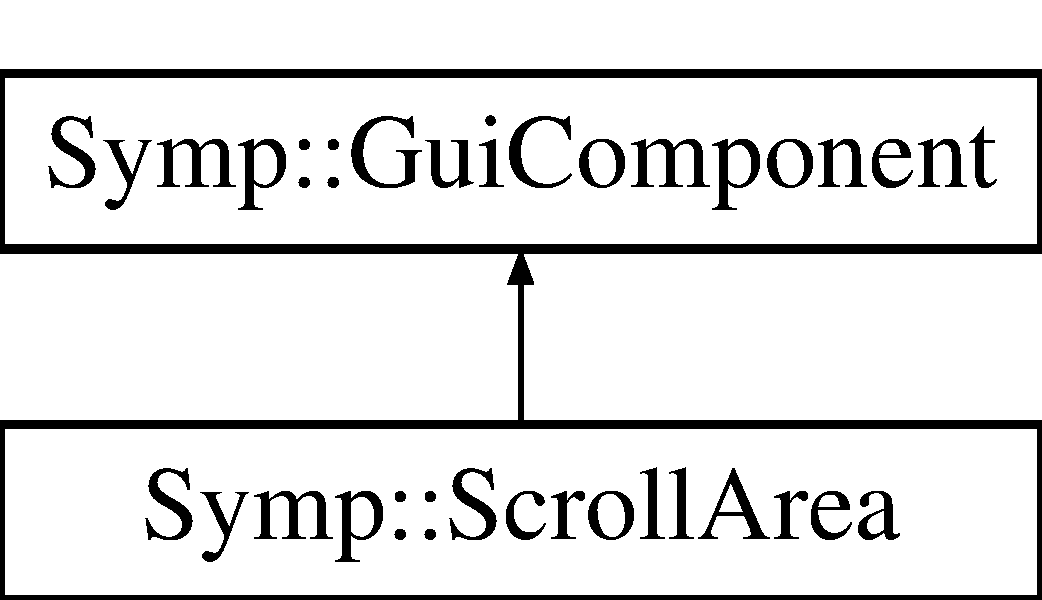
\includegraphics[height=2.000000cm]{class_symp_1_1_scroll_area}
\end{center}
\end{figure}
\subsection*{Public Member Functions}
\begin{DoxyCompactItemize}
\item 
\hyperlink{class_symp_1_1_scroll_area_ac6739b730ec0358cbb2feceb1c2f2dcf}{Scroll\-Area} ()
\item 
\hyperlink{class_symp_1_1_scroll_area_a42842f32256e6e2abd8008711028f039}{Scroll\-Area} (float i\-Pos\-X, float i\-Pos\-Y, int i\-Width, int i\-Height)
\item 
\hyperlink{class_symp_1_1_scroll_area_ab76e85e7c6888f1a319f87d7c5b83f9d}{$\sim$\-Scroll\-Area} ()
\item 
virtual void \hyperlink{class_symp_1_1_scroll_area_a9183e9193ecfa8a2d9fda6ff4d706680}{update} ()
\end{DoxyCompactItemize}
\subsection*{Additional Inherited Members}


\subsection{Detailed Description}
the \hyperlink{class_symp_1_1_gui_component_a22124675c2976983ac18374f81cc3fb3}{Gui\-Component} class The \hyperlink{class_symp_1_1_scroll_area_ac6739b730ec0358cbb2feceb1c2f2dcf}{Scroll\-Area} class is part of the menu graphical components and can be used only in the menu context. A \hyperlink{class_symp_1_1_scroll_area_ac6739b730ec0358cbb2feceb1c2f2dcf}{Scroll\-Area} can contain \hyperlink{class_symp_1_1_gui_component_a22124675c2976983ac18374f81cc3fb3}{Gui\-Component} and hide or show only a region of them. The \hyperlink{class_symp_1_1_scroll_area_ac6739b730ec0358cbb2feceb1c2f2dcf}{Scroll\-Area} is connected to a \#\-Slider for displacing the region shown. \begin{DoxyRefDesc}{Todo}
\item[\hyperlink{todo__todo000002}{Todo}]do the class \end{DoxyRefDesc}
\begin{DoxySeeAlso}{See Also}
\hyperlink{class_symp_1_1_menu_manager}{Menu\-Manager} 

\hyperlink{class_symp_1_1_slider}{Slider} 

\hyperlink{class_symp_1_1_gui_component}{Gui\-Component} 

\hyperlink{class_symp_1_1_scroll_area_ac6739b730ec0358cbb2feceb1c2f2dcf}{Scroll\-Area()} 

\hyperlink{class_symp_1_1_scroll_area_ab76e85e7c6888f1a319f87d7c5b83f9d}{$\sim$\-Scroll\-Area()} 
\end{DoxySeeAlso}


Definition at line 21 of file Scroll\-Area.\-h.



\subsection{Constructor \& Destructor Documentation}
\hypertarget{class_symp_1_1_scroll_area_ac6739b730ec0358cbb2feceb1c2f2dcf}{\index{Symp\-::\-Scroll\-Area@{Symp\-::\-Scroll\-Area}!Scroll\-Area@{Scroll\-Area}}
\index{Scroll\-Area@{Scroll\-Area}!Symp::ScrollArea@{Symp\-::\-Scroll\-Area}}
\subsubsection[{Scroll\-Area}]{\setlength{\rightskip}{0pt plus 5cm}Symp\-::\-Scroll\-Area\-::\-Scroll\-Area (
\begin{DoxyParamCaption}
{}
\end{DoxyParamCaption}
)}}\label{class_symp_1_1_scroll_area_ac6739b730ec0358cbb2feceb1c2f2dcf}


Definition at line 6 of file Scroll\-Area.\-cpp.

\hypertarget{class_symp_1_1_scroll_area_a42842f32256e6e2abd8008711028f039}{\index{Symp\-::\-Scroll\-Area@{Symp\-::\-Scroll\-Area}!Scroll\-Area@{Scroll\-Area}}
\index{Scroll\-Area@{Scroll\-Area}!Symp::ScrollArea@{Symp\-::\-Scroll\-Area}}
\subsubsection[{Scroll\-Area}]{\setlength{\rightskip}{0pt plus 5cm}Symp\-::\-Scroll\-Area\-::\-Scroll\-Area (
\begin{DoxyParamCaption}
\item[{float}]{i\-Pos\-X, }
\item[{float}]{i\-Pos\-Y, }
\item[{int}]{i\-Width, }
\item[{int}]{i\-Height}
\end{DoxyParamCaption}
)}}\label{class_symp_1_1_scroll_area_a42842f32256e6e2abd8008711028f039}


Definition at line 12 of file Scroll\-Area.\-cpp.

\hypertarget{class_symp_1_1_scroll_area_ab76e85e7c6888f1a319f87d7c5b83f9d}{\index{Symp\-::\-Scroll\-Area@{Symp\-::\-Scroll\-Area}!$\sim$\-Scroll\-Area@{$\sim$\-Scroll\-Area}}
\index{$\sim$\-Scroll\-Area@{$\sim$\-Scroll\-Area}!Symp::ScrollArea@{Symp\-::\-Scroll\-Area}}
\subsubsection[{$\sim$\-Scroll\-Area}]{\setlength{\rightskip}{0pt plus 5cm}Symp\-::\-Scroll\-Area\-::$\sim$\-Scroll\-Area (
\begin{DoxyParamCaption}
{}
\end{DoxyParamCaption}
)\hspace{0.3cm}{\ttfamily [inline]}}}\label{class_symp_1_1_scroll_area_ab76e85e7c6888f1a319f87d7c5b83f9d}


Definition at line 25 of file Scroll\-Area.\-h.



\subsection{Member Function Documentation}
\hypertarget{class_symp_1_1_scroll_area_a9183e9193ecfa8a2d9fda6ff4d706680}{\index{Symp\-::\-Scroll\-Area@{Symp\-::\-Scroll\-Area}!update@{update}}
\index{update@{update}!Symp::ScrollArea@{Symp\-::\-Scroll\-Area}}
\subsubsection[{update}]{\setlength{\rightskip}{0pt plus 5cm}virtual void Symp\-::\-Scroll\-Area\-::update (
\begin{DoxyParamCaption}
{}
\end{DoxyParamCaption}
)\hspace{0.3cm}{\ttfamily [inline]}, {\ttfamily [virtual]}}}\label{class_symp_1_1_scroll_area_a9183e9193ecfa8a2d9fda6ff4d706680}


Implements \hyperlink{class_symp_1_1_gui_component_add73e07ea0a3c9c1c90640e783a3b5de}{Symp\-::\-Gui\-Component}.



Definition at line 27 of file Scroll\-Area.\-h.



The documentation for this class was generated from the following files\-:\begin{DoxyCompactItemize}
\item 
/home/cecilia/\-Documents/\-Symptogen/src/menu/\hyperlink{_scroll_area_8h}{Scroll\-Area.\-h}\item 
/home/cecilia/\-Documents/\-Symptogen/src/menu/\hyperlink{_scroll_area_8cpp}{Scroll\-Area.\-cpp}\end{DoxyCompactItemize}

\hypertarget{class_symp_1_1_singleton}{\section{Symp\-:\-:Singleton$<$ T $>$ Class Template Reference}
\label{class_symp_1_1_singleton}\index{Symp\-::\-Singleton$<$ T $>$@{Symp\-::\-Singleton$<$ T $>$}}
}


{\ttfamily \#include $<$Singleton.\-h$>$}

\subsection*{Static Public Member Functions}
\begin{DoxyCompactItemize}
\item 
static T $\ast$ \hyperlink{class_symp_1_1_singleton_a2412fc841373411011479fe1da688fe1}{get\-Instance} ()
\item 
static void \hyperlink{class_symp_1_1_singleton_a38a9bdf838d0af33492f817319045751}{remove\-Instance} ()
\end{DoxyCompactItemize}
\subsection*{Protected Member Functions}
\begin{DoxyCompactItemize}
\item 
\hyperlink{class_symp_1_1_singleton_afe7a7830bed6c0ab39ddb6c1ca9f5a17}{Singleton} ()
\item 
\hyperlink{class_symp_1_1_singleton_aae7ca2a642d9c8486c34f5862b6dcfb5}{$\sim$\-Singleton} ()
\end{DoxyCompactItemize}


\subsection{Detailed Description}
\subsubsection*{template$<$typename T$>$class Symp\-::\-Singleton$<$ T $>$}



Definition at line 9 of file Singleton.\-h.



\subsection{Constructor \& Destructor Documentation}
\hypertarget{class_symp_1_1_singleton_afe7a7830bed6c0ab39ddb6c1ca9f5a17}{\index{Symp\-::\-Singleton@{Symp\-::\-Singleton}!Singleton@{Singleton}}
\index{Singleton@{Singleton}!Symp::Singleton@{Symp\-::\-Singleton}}
\subsubsection[{Singleton}]{\setlength{\rightskip}{0pt plus 5cm}template$<$typename T$>$ {\bf Symp\-::\-Singleton}$<$ T $>$\-::{\bf Singleton} (
\begin{DoxyParamCaption}
{}
\end{DoxyParamCaption}
)\hspace{0.3cm}{\ttfamily [inline]}, {\ttfamily [protected]}}}\label{class_symp_1_1_singleton_afe7a7830bed6c0ab39ddb6c1ca9f5a17}
Constructor 

Definition at line 15 of file Singleton.\-h.

\hypertarget{class_symp_1_1_singleton_aae7ca2a642d9c8486c34f5862b6dcfb5}{\index{Symp\-::\-Singleton@{Symp\-::\-Singleton}!$\sim$\-Singleton@{$\sim$\-Singleton}}
\index{$\sim$\-Singleton@{$\sim$\-Singleton}!Symp::Singleton@{Symp\-::\-Singleton}}
\subsubsection[{$\sim$\-Singleton}]{\setlength{\rightskip}{0pt plus 5cm}template$<$typename T$>$ {\bf Symp\-::\-Singleton}$<$ T $>$\-::$\sim${\bf Singleton} (
\begin{DoxyParamCaption}
{}
\end{DoxyParamCaption}
)\hspace{0.3cm}{\ttfamily [inline]}, {\ttfamily [protected]}}}\label{class_symp_1_1_singleton_aae7ca2a642d9c8486c34f5862b6dcfb5}
Destructor 

Definition at line 20 of file Singleton.\-h.



\subsection{Member Function Documentation}
\hypertarget{class_symp_1_1_singleton_a2412fc841373411011479fe1da688fe1}{\index{Symp\-::\-Singleton@{Symp\-::\-Singleton}!get\-Instance@{get\-Instance}}
\index{get\-Instance@{get\-Instance}!Symp::Singleton@{Symp\-::\-Singleton}}
\subsubsection[{get\-Instance}]{\setlength{\rightskip}{0pt plus 5cm}template$<$typename T$>$ static T$\ast$ {\bf Symp\-::\-Singleton}$<$ T $>$\-::get\-Instance (
\begin{DoxyParamCaption}
{}
\end{DoxyParamCaption}
)\hspace{0.3cm}{\ttfamily [inline]}, {\ttfamily [static]}}}\label{class_symp_1_1_singleton_a2412fc841373411011479fe1da688fe1}
Return the singleton \begin{DoxyReturn}{Returns}
T$\ast$ \-: the instance of the singleton T 
\end{DoxyReturn}
\begin{DoxySeeAlso}{See Also}
\hyperlink{class_symp_1_1_singleton_a2412fc841373411011479fe1da688fe1}{get\-Instance()} 

\hyperlink{class_symp_1_1_singleton_a38a9bdf838d0af33492f817319045751}{remove\-Instance()} 
\end{DoxySeeAlso}


Definition at line 30 of file Singleton.\-h.

\hypertarget{class_symp_1_1_singleton_a38a9bdf838d0af33492f817319045751}{\index{Symp\-::\-Singleton@{Symp\-::\-Singleton}!remove\-Instance@{remove\-Instance}}
\index{remove\-Instance@{remove\-Instance}!Symp::Singleton@{Symp\-::\-Singleton}}
\subsubsection[{remove\-Instance}]{\setlength{\rightskip}{0pt plus 5cm}template$<$typename T$>$ static void {\bf Symp\-::\-Singleton}$<$ T $>$\-::remove\-Instance (
\begin{DoxyParamCaption}
{}
\end{DoxyParamCaption}
)\hspace{0.3cm}{\ttfamily [inline]}, {\ttfamily [static]}}}\label{class_symp_1_1_singleton_a38a9bdf838d0af33492f817319045751}
Remove the singleton \begin{DoxySeeAlso}{See Also}
\hyperlink{class_symp_1_1_singleton_a2412fc841373411011479fe1da688fe1}{get\-Instance()} 

\hyperlink{class_symp_1_1_singleton_a38a9bdf838d0af33492f817319045751}{remove\-Instance()} 
\end{DoxySeeAlso}


Definition at line 43 of file Singleton.\-h.



The documentation for this class was generated from the following file\-:\begin{DoxyCompactItemize}
\item 
/home/cecilia/\-Documents/\-Symptogen/src/util/\hyperlink{_singleton_8h}{Singleton.\-h}\end{DoxyCompactItemize}

\hypertarget{class_symp_1_1_slider}{\section{Symp\-:\-:Slider Class Reference}
\label{class_symp_1_1_slider}\index{Symp\-::\-Slider@{Symp\-::\-Slider}}
}


{\ttfamily \#include $<$Slider.\-h$>$}

Inheritance diagram for Symp\-:\-:Slider\-:\begin{figure}[H]
\begin{center}
\leavevmode
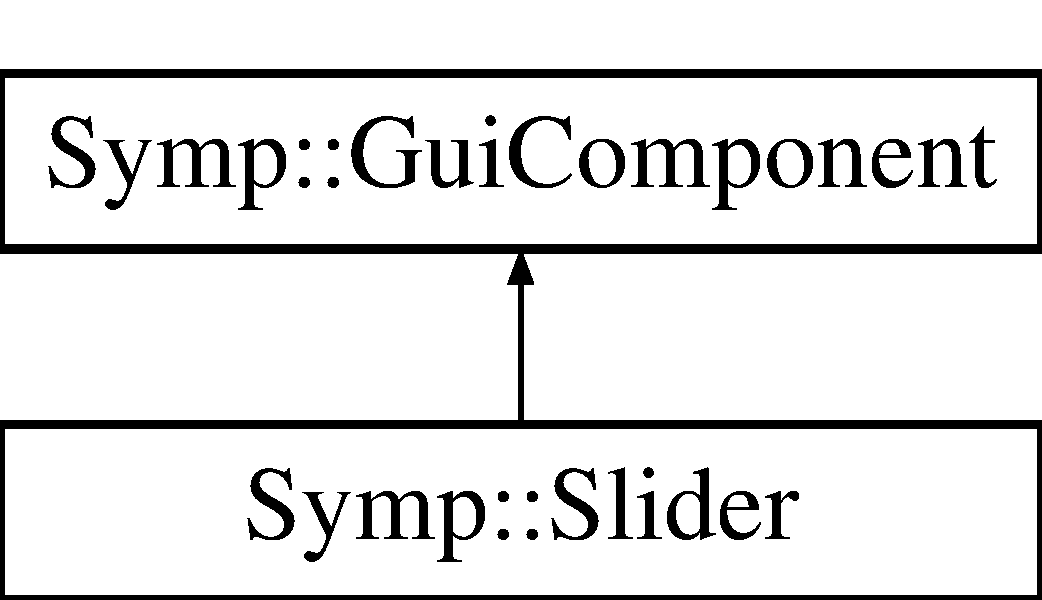
\includegraphics[height=2.000000cm]{class_symp_1_1_slider}
\end{center}
\end{figure}
\subsection*{Public Member Functions}
\begin{DoxyCompactItemize}
\item 
\hyperlink{class_symp_1_1_slider_a4ebcc86ae45c76bf855ec8aa483e44ce}{Slider} (float percentage, float i\-Pos\-X=0, float i\-Pos\-Y=0, int i\-Width=0, int i\-Height=0)
\begin{DoxyCompactList}\small\item\em \hyperlink{class_symp_1_1_slider}{Slider} constructor Responsible for the initialization of the private attributes of the \hyperlink{class_symp_1_1_slider_a4ebcc86ae45c76bf855ec8aa483e44ce}{Slider} class. \end{DoxyCompactList}\item 
\hyperlink{class_symp_1_1_slider_a784b39c5691fff0d3e84e1b3da7177f9}{$\sim$\-Slider} ()
\item 
virtual void \hyperlink{class_symp_1_1_slider_ab010de4ff23eef8a6cc6706e9902209f}{update} ()
\begin{DoxyCompactList}\small\item\em \hyperlink{class_symp_1_1_slider}{Slider} update fonction Refresh the display of the \hyperlink{class_symp_1_1_slider_a4ebcc86ae45c76bf855ec8aa483e44ce}{Slider}. \end{DoxyCompactList}\item 
void \hyperlink{class_symp_1_1_slider_a7e0c531c24bbf7f2dad81fbf98e43601}{fill} (\hyperlink{struct_symp_1_1_color}{Color} color)
\begin{DoxyCompactList}\small\item\em fill \hyperlink{class_symp_1_1_slider}{Slider}'s background function \end{DoxyCompactList}\item 
void \hyperlink{class_symp_1_1_slider_a77c00c6e35179757339f73fd2494502b}{set\-Percentage} (float f\-Percentage)
\item 
\hyperlink{class_symp_1_1_image}{Image} $\ast$ \hyperlink{class_symp_1_1_slider_a0204fb89e780be4ddd4fc41379d9c463}{get\-Image} () const 
\item 
float \hyperlink{class_symp_1_1_slider_a454537b48768334a5c81f84c9af2b006}{get\-Percentage} () const 
\end{DoxyCompactItemize}
\subsection*{Additional Inherited Members}


\subsection{Detailed Description}
the \hyperlink{class_symp_1_1_gui_component_a22124675c2976983ac18374f81cc3fb3}{Gui\-Component} class The \hyperlink{class_symp_1_1_slider_a4ebcc86ae45c76bf855ec8aa483e44ce}{Slider} class is part of the menu graphical components and can be used only in the menu context. A \hyperlink{class_symp_1_1_slider_a4ebcc86ae45c76bf855ec8aa483e44ce}{Slider} can used in two situation \-: for displaying a progression, or as an event receiver for a collaboration with a \#\-Scroll\-Area. The \hyperlink{class_symp_1_1_slider_a4ebcc86ae45c76bf855ec8aa483e44ce}{Slider} is composed of a primitive associated with a texture. Only a texture, or a Indielib I\-N\-D\-\_\-\-Surface can have a specific region shown. The image part of the \hyperlink{class_symp_1_1_slider_a4ebcc86ae45c76bf855ec8aa483e44ce}{Slider} must be added separatly to the \#\-Menu\-Manager for being displayed. \begin{DoxySeeAlso}{See Also}
\hyperlink{class_symp_1_1_menu_manager}{Menu\-Manager} 

\hyperlink{class_symp_1_1_gui_component}{Gui\-Component} 

\hyperlink{class_symp_1_1_slider_a4ebcc86ae45c76bf855ec8aa483e44ce}{Slider()} 

\hyperlink{class_symp_1_1_slider_a784b39c5691fff0d3e84e1b3da7177f9}{$\sim$\-Slider()} 
\end{DoxySeeAlso}


Definition at line 22 of file Slider.\-h.



\subsection{Constructor \& Destructor Documentation}
\hypertarget{class_symp_1_1_slider_a4ebcc86ae45c76bf855ec8aa483e44ce}{\index{Symp\-::\-Slider@{Symp\-::\-Slider}!Slider@{Slider}}
\index{Slider@{Slider}!Symp::Slider@{Symp\-::\-Slider}}
\subsubsection[{Slider}]{\setlength{\rightskip}{0pt plus 5cm}Symp\-::\-Slider\-::\-Slider (
\begin{DoxyParamCaption}
\item[{float}]{f\-Percentage, }
\item[{float}]{i\-Pos\-X = {\ttfamily 0}, }
\item[{float}]{i\-Pos\-Y = {\ttfamily 0}, }
\item[{int}]{i\-Width = {\ttfamily 0}, }
\item[{int}]{i\-Height = {\ttfamily 0}}
\end{DoxyParamCaption}
)}}\label{class_symp_1_1_slider_a4ebcc86ae45c76bf855ec8aa483e44ce}


\hyperlink{class_symp_1_1_slider}{Slider} constructor Responsible for the initialization of the private attributes of the \hyperlink{class_symp_1_1_slider_a4ebcc86ae45c76bf855ec8aa483e44ce}{Slider} class. 


\begin{DoxyParams}{Parameters}
{\em f\-Percentage} & the size of the foreground \#\-Image \\
\hline
{\em i\-Pos\-X} & the x coordinate of the upper-\/left corner of the \hyperlink{class_symp_1_1_slider_a4ebcc86ae45c76bf855ec8aa483e44ce}{Slider} in pixels \\
\hline
{\em i\-Pos\-Y} & the y coordinate of the upper-\/left corner of the \hyperlink{class_symp_1_1_slider_a4ebcc86ae45c76bf855ec8aa483e44ce}{Slider} in pixels \\
\hline
{\em i\-Width} & the width of the \hyperlink{class_symp_1_1_slider_a4ebcc86ae45c76bf855ec8aa483e44ce}{Slider} in pixels \\
\hline
{\em i\-Height} & the height of the \hyperlink{class_symp_1_1_slider_a4ebcc86ae45c76bf855ec8aa483e44ce}{Slider} in pixels \\
\hline
\end{DoxyParams}
\begin{DoxySeeAlso}{See Also}
\hyperlink{class_symp_1_1_player}{Player} 

\hyperlink{class_symp_1_1_scroll_area}{Scroll\-Area} 

\hyperlink{class_symp_1_1_menu_manager}{Menu\-Manager} 

\hyperlink{class_symp_1_1_gui_component}{Gui\-Component} 

\hyperlink{class_symp_1_1_gui_component_a05838e01bbf1e31f292ed4b92a520f20}{init()} 

\hyperlink{class_symp_1_1_slider_a784b39c5691fff0d3e84e1b3da7177f9}{$\sim$\-Slider()} 
\end{DoxySeeAlso}


Definition at line 22 of file Slider.\-cpp.

\hypertarget{class_symp_1_1_slider_a784b39c5691fff0d3e84e1b3da7177f9}{\index{Symp\-::\-Slider@{Symp\-::\-Slider}!$\sim$\-Slider@{$\sim$\-Slider}}
\index{$\sim$\-Slider@{$\sim$\-Slider}!Symp::Slider@{Symp\-::\-Slider}}
\subsubsection[{$\sim$\-Slider}]{\setlength{\rightskip}{0pt plus 5cm}Symp\-::\-Slider\-::$\sim$\-Slider (
\begin{DoxyParamCaption}
{}
\end{DoxyParamCaption}
)}}\label{class_symp_1_1_slider_a784b39c5691fff0d3e84e1b3da7177f9}


\subsection{Member Function Documentation}
\hypertarget{class_symp_1_1_slider_a7e0c531c24bbf7f2dad81fbf98e43601}{\index{Symp\-::\-Slider@{Symp\-::\-Slider}!fill@{fill}}
\index{fill@{fill}!Symp::Slider@{Symp\-::\-Slider}}
\subsubsection[{fill}]{\setlength{\rightskip}{0pt plus 5cm}void Symp\-::\-Slider\-::fill (
\begin{DoxyParamCaption}
\item[{{\bf Symp\-::\-Color}}]{color}
\end{DoxyParamCaption}
)}}\label{class_symp_1_1_slider_a7e0c531c24bbf7f2dad81fbf98e43601}


fill \hyperlink{class_symp_1_1_slider}{Slider}'s background function 

\begin{DoxySeeAlso}{See Also}
\hyperlink{class_symp_1_1_slider}{Slider} 

\hyperlink{class_symp_1_1_slider_a784b39c5691fff0d3e84e1b3da7177f9}{$\sim$\-Slider()} 

\hyperlink{struct_symp_1_1_color}{Color} 

\hyperlink{class_symp_1_1_gui_component}{Gui\-Component} 
\end{DoxySeeAlso}


Definition at line 74 of file Slider.\-cpp.

\hypertarget{class_symp_1_1_slider_a0204fb89e780be4ddd4fc41379d9c463}{\index{Symp\-::\-Slider@{Symp\-::\-Slider}!get\-Image@{get\-Image}}
\index{get\-Image@{get\-Image}!Symp::Slider@{Symp\-::\-Slider}}
\subsubsection[{get\-Image}]{\setlength{\rightskip}{0pt plus 5cm}{\bf Image}$\ast$ Symp\-::\-Slider\-::get\-Image (
\begin{DoxyParamCaption}
{}
\end{DoxyParamCaption}
) const\hspace{0.3cm}{\ttfamily [inline]}}}\label{class_symp_1_1_slider_a0204fb89e780be4ddd4fc41379d9c463}


Definition at line 35 of file Slider.\-h.

\hypertarget{class_symp_1_1_slider_a454537b48768334a5c81f84c9af2b006}{\index{Symp\-::\-Slider@{Symp\-::\-Slider}!get\-Percentage@{get\-Percentage}}
\index{get\-Percentage@{get\-Percentage}!Symp::Slider@{Symp\-::\-Slider}}
\subsubsection[{get\-Percentage}]{\setlength{\rightskip}{0pt plus 5cm}float Symp\-::\-Slider\-::get\-Percentage (
\begin{DoxyParamCaption}
{}
\end{DoxyParamCaption}
) const\hspace{0.3cm}{\ttfamily [inline]}}}\label{class_symp_1_1_slider_a454537b48768334a5c81f84c9af2b006}


Definition at line 36 of file Slider.\-h.

\hypertarget{class_symp_1_1_slider_a77c00c6e35179757339f73fd2494502b}{\index{Symp\-::\-Slider@{Symp\-::\-Slider}!set\-Percentage@{set\-Percentage}}
\index{set\-Percentage@{set\-Percentage}!Symp::Slider@{Symp\-::\-Slider}}
\subsubsection[{set\-Percentage}]{\setlength{\rightskip}{0pt plus 5cm}void Symp\-::\-Slider\-::set\-Percentage (
\begin{DoxyParamCaption}
\item[{float}]{f\-Percentage}
\end{DoxyParamCaption}
)\hspace{0.3cm}{\ttfamily [inline]}}}\label{class_symp_1_1_slider_a77c00c6e35179757339f73fd2494502b}


Definition at line 32 of file Slider.\-h.

\hypertarget{class_symp_1_1_slider_ab010de4ff23eef8a6cc6706e9902209f}{\index{Symp\-::\-Slider@{Symp\-::\-Slider}!update@{update}}
\index{update@{update}!Symp::Slider@{Symp\-::\-Slider}}
\subsubsection[{update}]{\setlength{\rightskip}{0pt plus 5cm}void Symp\-::\-Slider\-::update (
\begin{DoxyParamCaption}
{}
\end{DoxyParamCaption}
)\hspace{0.3cm}{\ttfamily [virtual]}}}\label{class_symp_1_1_slider_ab010de4ff23eef8a6cc6706e9902209f}


\hyperlink{class_symp_1_1_slider}{Slider} update fonction Refresh the display of the \hyperlink{class_symp_1_1_slider_a4ebcc86ae45c76bf855ec8aa483e44ce}{Slider}. 

\begin{DoxySeeAlso}{See Also}
\hyperlink{class_symp_1_1_slider}{Slider} 

\hyperlink{class_symp_1_1_slider_a784b39c5691fff0d3e84e1b3da7177f9}{$\sim$\-Slider()} 

\hyperlink{class_symp_1_1_gui_component}{Gui\-Component} 
\end{DoxySeeAlso}


Implements \hyperlink{class_symp_1_1_gui_component_add73e07ea0a3c9c1c90640e783a3b5de}{Symp\-::\-Gui\-Component}.



Definition at line 54 of file Slider.\-cpp.



The documentation for this class was generated from the following files\-:\begin{DoxyCompactItemize}
\item 
/home/cecilia/\-Documents/\-Symptogen/src/menu/\hyperlink{_slider_8h}{Slider.\-h}\item 
/home/cecilia/\-Documents/\-Symptogen/src/menu/\hyperlink{_slider_8cpp}{Slider.\-cpp}\end{DoxyCompactItemize}

\hypertarget{class_symp_1_1_sneeze}{\section{Symp\-:\-:Sneeze Class Reference}
\label{class_symp_1_1_sneeze}\index{Symp\-::\-Sneeze@{Symp\-::\-Sneeze}}
}


{\ttfamily \#include $<$Sneeze.\-h$>$}

Inheritance diagram for Symp\-:\-:Sneeze\-:\begin{figure}[H]
\begin{center}
\leavevmode
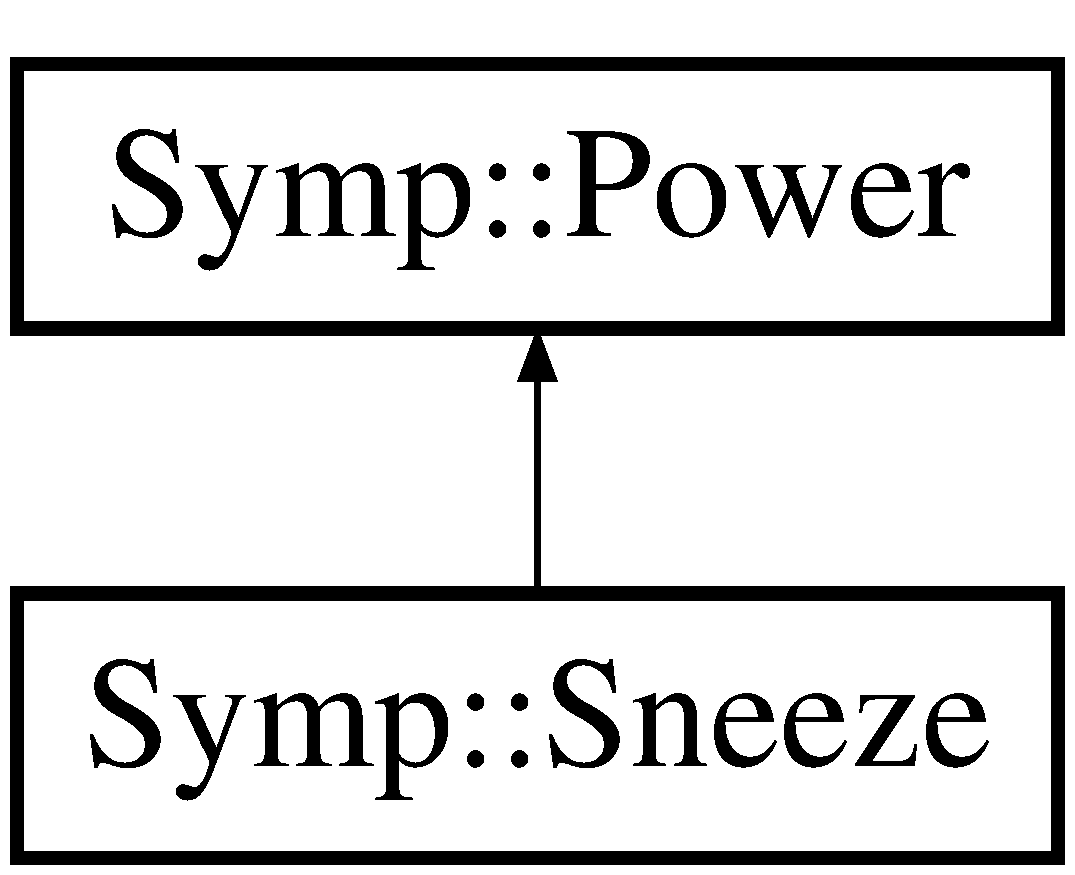
\includegraphics[height=2.000000cm]{class_symp_1_1_sneeze}
\end{center}
\end{figure}
\subsection*{Public Member Functions}
\begin{DoxyCompactItemize}
\item 
\hyperlink{class_symp_1_1_sneeze_a13fbccbd6a1f4cf90e5dec41ace022c8}{Sneeze} ()
\begin{DoxyCompactList}\small\item\em \hyperlink{class_symp_1_1_sneeze}{Sneeze} class constructor. \end{DoxyCompactList}\item 
\hyperlink{class_symp_1_1_sneeze_aad72c8ab50d872b9dcdb1e8cab38755e}{$\sim$\-Sneeze} ()
\begin{DoxyCompactList}\small\item\em \hyperlink{class_symp_1_1_sneeze}{Sneeze} class destructor. \end{DoxyCompactList}\item 
void \hyperlink{class_symp_1_1_sneeze_aaaf79da47ab1a8888f4af276e31087f1}{execute} ()
\begin{DoxyCompactList}\small\item\em Implementation of the \hyperlink{class_symp_1_1_power}{Power} abstract class If the sneeze power is activated, this method will be called at each turn of the main loop. This method will make the character sneeze, or not. When the time since the last sneeze exceeds \#m\-\_\-ui\-Time\-To\-Trigger\-Random\-Sneeze, the random sneeze is activated and the more time elapses, the more the probability of sneezing increases. \end{DoxyCompactList}\item 
void \hyperlink{class_symp_1_1_sneeze_a76aec7dca3104e9e0b8c2dade0d9eac9}{force\-Execution} ()
\begin{DoxyCompactList}\small\item\em Force the execution of the sneeze, regardless of m\-\_\-ui\-Last\-Execution. This method is called when we want to force the execution of the sneeze, regardless of the randomm calculation. It is used to trigger the sneeze when the Dino encounters a flower. \end{DoxyCompactList}\item 
void \hyperlink{class_symp_1_1_sneeze_aafc16f638a08e04c171944adfef888b2}{update\-Power\-Timer} ()
\begin{DoxyCompactList}\small\item\em Update the timer of the power This method is called when the power animation begin, it is used to know when the animation begin and when it end. \end{DoxyCompactList}\item 
unsigned int \hyperlink{class_symp_1_1_sneeze_aaa1bcec0f27ca46fc99c8f19a58a11e1}{get\-Last\-Execution} () const 
\item 
unsigned int \hyperlink{class_symp_1_1_sneeze_a5e0528e0c55ea2a7f8ad23540c9486ff}{get\-Repulsion\-Strength} () const 
\item 
unsigned int \hyperlink{class_symp_1_1_sneeze_a5e777bc98532683cb94b8d0c514c9a88}{get\-Time\-To\-Trigger\-Random\-Sneeze} () const 
\item 
bool \hyperlink{class_symp_1_1_sneeze_a3b3d7cd2d72c8fd371b1766b7ba3285f}{is\-Warning\-Sneeze} () const 
\item 
bool \hyperlink{class_symp_1_1_sneeze_a4d1261972072ed5da8bce9c7dd099cf0}{is\-Sneezing} () const 
\item 
void \hyperlink{class_symp_1_1_sneeze_a6f611cb36b4cbcaf44759ac87040171a}{set\-Repulsion\-Strength} (unsigned int rs)
\item 
void \hyperlink{class_symp_1_1_sneeze_abef3d3a4ad922ab1c54899e19f17bdcc}{set\-Time\-To\-Trigger\-Random\-Sneeze} (unsigned int tttrs)
\end{DoxyCompactItemize}
\subsection*{Additional Inherited Members}


\subsection{Detailed Description}


Definition at line 9 of file Sneeze.\-h.



\subsection{Constructor \& Destructor Documentation}
\hypertarget{class_symp_1_1_sneeze_a13fbccbd6a1f4cf90e5dec41ace022c8}{\index{Symp\-::\-Sneeze@{Symp\-::\-Sneeze}!Sneeze@{Sneeze}}
\index{Sneeze@{Sneeze}!Symp::Sneeze@{Symp\-::\-Sneeze}}
\subsubsection[{Sneeze}]{\setlength{\rightskip}{0pt plus 5cm}Symp\-::\-Sneeze\-::\-Sneeze (
\begin{DoxyParamCaption}
{}
\end{DoxyParamCaption}
)\hspace{0.3cm}{\ttfamily [inline]}}}\label{class_symp_1_1_sneeze_a13fbccbd6a1f4cf90e5dec41ace022c8}


\hyperlink{class_symp_1_1_sneeze}{Sneeze} class constructor. 



Definition at line 16 of file Sneeze.\-h.

\hypertarget{class_symp_1_1_sneeze_aad72c8ab50d872b9dcdb1e8cab38755e}{\index{Symp\-::\-Sneeze@{Symp\-::\-Sneeze}!$\sim$\-Sneeze@{$\sim$\-Sneeze}}
\index{$\sim$\-Sneeze@{$\sim$\-Sneeze}!Symp::Sneeze@{Symp\-::\-Sneeze}}
\subsubsection[{$\sim$\-Sneeze}]{\setlength{\rightskip}{0pt plus 5cm}Symp\-::\-Sneeze\-::$\sim$\-Sneeze (
\begin{DoxyParamCaption}
{}
\end{DoxyParamCaption}
)\hspace{0.3cm}{\ttfamily [inline]}}}\label{class_symp_1_1_sneeze_aad72c8ab50d872b9dcdb1e8cab38755e}


\hyperlink{class_symp_1_1_sneeze}{Sneeze} class destructor. 



Definition at line 25 of file Sneeze.\-h.



\subsection{Member Function Documentation}
\hypertarget{class_symp_1_1_sneeze_aaaf79da47ab1a8888f4af276e31087f1}{\index{Symp\-::\-Sneeze@{Symp\-::\-Sneeze}!execute@{execute}}
\index{execute@{execute}!Symp::Sneeze@{Symp\-::\-Sneeze}}
\subsubsection[{execute}]{\setlength{\rightskip}{0pt plus 5cm}void Symp\-::\-Sneeze\-::execute (
\begin{DoxyParamCaption}
{}
\end{DoxyParamCaption}
)\hspace{0.3cm}{\ttfamily [virtual]}}}\label{class_symp_1_1_sneeze_aaaf79da47ab1a8888f4af276e31087f1}


Implementation of the \hyperlink{class_symp_1_1_power}{Power} abstract class If the sneeze power is activated, this method will be called at each turn of the main loop. This method will make the character sneeze, or not. When the time since the last sneeze exceeds \#m\-\_\-ui\-Time\-To\-Trigger\-Random\-Sneeze, the random sneeze is activated and the more time elapses, the more the probability of sneezing increases. 



Reimplemented from \hyperlink{class_symp_1_1_power_a148a017c9f01bea343d062460074eae5}{Symp\-::\-Power}.



Definition at line 11 of file Sneeze.\-cpp.

\hypertarget{class_symp_1_1_sneeze_a76aec7dca3104e9e0b8c2dade0d9eac9}{\index{Symp\-::\-Sneeze@{Symp\-::\-Sneeze}!force\-Execution@{force\-Execution}}
\index{force\-Execution@{force\-Execution}!Symp::Sneeze@{Symp\-::\-Sneeze}}
\subsubsection[{force\-Execution}]{\setlength{\rightskip}{0pt plus 5cm}void Symp\-::\-Sneeze\-::force\-Execution (
\begin{DoxyParamCaption}
{}
\end{DoxyParamCaption}
)\hspace{0.3cm}{\ttfamily [virtual]}}}\label{class_symp_1_1_sneeze_a76aec7dca3104e9e0b8c2dade0d9eac9}


Force the execution of the sneeze, regardless of m\-\_\-ui\-Last\-Execution. This method is called when we want to force the execution of the sneeze, regardless of the randomm calculation. It is used to trigger the sneeze when the Dino encounters a flower. 



Reimplemented from \hyperlink{class_symp_1_1_power_acc825d941b947be435944fc4d876a118}{Symp\-::\-Power}.



Definition at line 41 of file Sneeze.\-cpp.

\hypertarget{class_symp_1_1_sneeze_aaa1bcec0f27ca46fc99c8f19a58a11e1}{\index{Symp\-::\-Sneeze@{Symp\-::\-Sneeze}!get\-Last\-Execution@{get\-Last\-Execution}}
\index{get\-Last\-Execution@{get\-Last\-Execution}!Symp::Sneeze@{Symp\-::\-Sneeze}}
\subsubsection[{get\-Last\-Execution}]{\setlength{\rightskip}{0pt plus 5cm}unsigned int Symp\-::\-Sneeze\-::get\-Last\-Execution (
\begin{DoxyParamCaption}
{}
\end{DoxyParamCaption}
) const\hspace{0.3cm}{\ttfamily [inline]}}}\label{class_symp_1_1_sneeze_aaa1bcec0f27ca46fc99c8f19a58a11e1}
Getters 

Definition at line 50 of file Sneeze.\-h.

\hypertarget{class_symp_1_1_sneeze_a5e0528e0c55ea2a7f8ad23540c9486ff}{\index{Symp\-::\-Sneeze@{Symp\-::\-Sneeze}!get\-Repulsion\-Strength@{get\-Repulsion\-Strength}}
\index{get\-Repulsion\-Strength@{get\-Repulsion\-Strength}!Symp::Sneeze@{Symp\-::\-Sneeze}}
\subsubsection[{get\-Repulsion\-Strength}]{\setlength{\rightskip}{0pt plus 5cm}unsigned int Symp\-::\-Sneeze\-::get\-Repulsion\-Strength (
\begin{DoxyParamCaption}
{}
\end{DoxyParamCaption}
) const\hspace{0.3cm}{\ttfamily [inline]}}}\label{class_symp_1_1_sneeze_a5e0528e0c55ea2a7f8ad23540c9486ff}


Definition at line 51 of file Sneeze.\-h.

\hypertarget{class_symp_1_1_sneeze_a5e777bc98532683cb94b8d0c514c9a88}{\index{Symp\-::\-Sneeze@{Symp\-::\-Sneeze}!get\-Time\-To\-Trigger\-Random\-Sneeze@{get\-Time\-To\-Trigger\-Random\-Sneeze}}
\index{get\-Time\-To\-Trigger\-Random\-Sneeze@{get\-Time\-To\-Trigger\-Random\-Sneeze}!Symp::Sneeze@{Symp\-::\-Sneeze}}
\subsubsection[{get\-Time\-To\-Trigger\-Random\-Sneeze}]{\setlength{\rightskip}{0pt plus 5cm}unsigned int Symp\-::\-Sneeze\-::get\-Time\-To\-Trigger\-Random\-Sneeze (
\begin{DoxyParamCaption}
{}
\end{DoxyParamCaption}
) const\hspace{0.3cm}{\ttfamily [inline]}}}\label{class_symp_1_1_sneeze_a5e777bc98532683cb94b8d0c514c9a88}


Definition at line 52 of file Sneeze.\-h.

\hypertarget{class_symp_1_1_sneeze_a4d1261972072ed5da8bce9c7dd099cf0}{\index{Symp\-::\-Sneeze@{Symp\-::\-Sneeze}!is\-Sneezing@{is\-Sneezing}}
\index{is\-Sneezing@{is\-Sneezing}!Symp::Sneeze@{Symp\-::\-Sneeze}}
\subsubsection[{is\-Sneezing}]{\setlength{\rightskip}{0pt plus 5cm}bool Symp\-::\-Sneeze\-::is\-Sneezing (
\begin{DoxyParamCaption}
{}
\end{DoxyParamCaption}
) const\hspace{0.3cm}{\ttfamily [inline]}}}\label{class_symp_1_1_sneeze_a4d1261972072ed5da8bce9c7dd099cf0}


Definition at line 55 of file Sneeze.\-h.

\hypertarget{class_symp_1_1_sneeze_a3b3d7cd2d72c8fd371b1766b7ba3285f}{\index{Symp\-::\-Sneeze@{Symp\-::\-Sneeze}!is\-Warning\-Sneeze@{is\-Warning\-Sneeze}}
\index{is\-Warning\-Sneeze@{is\-Warning\-Sneeze}!Symp::Sneeze@{Symp\-::\-Sneeze}}
\subsubsection[{is\-Warning\-Sneeze}]{\setlength{\rightskip}{0pt plus 5cm}bool Symp\-::\-Sneeze\-::is\-Warning\-Sneeze (
\begin{DoxyParamCaption}
{}
\end{DoxyParamCaption}
) const\hspace{0.3cm}{\ttfamily [inline]}}}\label{class_symp_1_1_sneeze_a3b3d7cd2d72c8fd371b1766b7ba3285f}


Definition at line 54 of file Sneeze.\-h.

\hypertarget{class_symp_1_1_sneeze_a6f611cb36b4cbcaf44759ac87040171a}{\index{Symp\-::\-Sneeze@{Symp\-::\-Sneeze}!set\-Repulsion\-Strength@{set\-Repulsion\-Strength}}
\index{set\-Repulsion\-Strength@{set\-Repulsion\-Strength}!Symp::Sneeze@{Symp\-::\-Sneeze}}
\subsubsection[{set\-Repulsion\-Strength}]{\setlength{\rightskip}{0pt plus 5cm}void Symp\-::\-Sneeze\-::set\-Repulsion\-Strength (
\begin{DoxyParamCaption}
\item[{unsigned int}]{rs}
\end{DoxyParamCaption}
)\hspace{0.3cm}{\ttfamily [inline]}}}\label{class_symp_1_1_sneeze_a6f611cb36b4cbcaf44759ac87040171a}
Setters 

Definition at line 60 of file Sneeze.\-h.

\hypertarget{class_symp_1_1_sneeze_abef3d3a4ad922ab1c54899e19f17bdcc}{\index{Symp\-::\-Sneeze@{Symp\-::\-Sneeze}!set\-Time\-To\-Trigger\-Random\-Sneeze@{set\-Time\-To\-Trigger\-Random\-Sneeze}}
\index{set\-Time\-To\-Trigger\-Random\-Sneeze@{set\-Time\-To\-Trigger\-Random\-Sneeze}!Symp::Sneeze@{Symp\-::\-Sneeze}}
\subsubsection[{set\-Time\-To\-Trigger\-Random\-Sneeze}]{\setlength{\rightskip}{0pt plus 5cm}void Symp\-::\-Sneeze\-::set\-Time\-To\-Trigger\-Random\-Sneeze (
\begin{DoxyParamCaption}
\item[{unsigned int}]{tttrs}
\end{DoxyParamCaption}
)\hspace{0.3cm}{\ttfamily [inline]}}}\label{class_symp_1_1_sneeze_abef3d3a4ad922ab1c54899e19f17bdcc}


Definition at line 61 of file Sneeze.\-h.

\hypertarget{class_symp_1_1_sneeze_aafc16f638a08e04c171944adfef888b2}{\index{Symp\-::\-Sneeze@{Symp\-::\-Sneeze}!update\-Power\-Timer@{update\-Power\-Timer}}
\index{update\-Power\-Timer@{update\-Power\-Timer}!Symp::Sneeze@{Symp\-::\-Sneeze}}
\subsubsection[{update\-Power\-Timer}]{\setlength{\rightskip}{0pt plus 5cm}void Symp\-::\-Sneeze\-::update\-Power\-Timer (
\begin{DoxyParamCaption}
{}
\end{DoxyParamCaption}
)}}\label{class_symp_1_1_sneeze_aafc16f638a08e04c171944adfef888b2}


Update the timer of the power This method is called when the power animation begin, it is used to know when the animation begin and when it end. 



The documentation for this class was generated from the following files\-:\begin{DoxyCompactItemize}
\item 
/home/cecilia/\-Documents/\-Symptogen/src/power/\hyperlink{_sneeze_8h}{Sneeze.\-h}\item 
/home/cecilia/\-Documents/\-Symptogen/src/power/\hyperlink{_sneeze_8cpp}{Sneeze.\-cpp}\end{DoxyCompactItemize}

\hypertarget{class_symp_1_1_sound_entity}{\section{Symp\-:\-:Sound\-Entity Class Reference}
\label{class_symp_1_1_sound_entity}\index{Symp\-::\-Sound\-Entity@{Symp\-::\-Sound\-Entity}}
}


{\ttfamily \#include $<$Sound\-Entity.\-h$>$}

\subsection*{Public Member Functions}
\begin{DoxyCompactItemize}
\item 
\hyperlink{class_symp_1_1_sound_entity_ae96bbc7bfe94c4759111904ba84882c3}{Sound\-Entity} (const char $\ast$file\-Name)
\item 
\hyperlink{class_symp_1_1_sound_entity_a90e4f841f08e1d74b7fe6e7697c75fee}{$\sim$\-Sound\-Entity} ()
\item 
F\-M\-O\-D\-::\-Sound $\ast$ \hyperlink{class_symp_1_1_sound_entity_a61a5a9145c3a9a7a42d891de4667aca1}{get\-Sound} () const 
\item 
F\-M\-O\-D\-::\-Channel $\ast$ \hyperlink{class_symp_1_1_sound_entity_a1e737f226f11f3c2afd67011c19c1c0f}{get\-Channel} () const 
\item 
void \hyperlink{class_symp_1_1_sound_entity_a4cccf6833eef1dbae8b2afae193cdb19}{set\-Channel} (F\-M\-O\-D\-::\-Channel $\ast$p\-Channel)
\end{DoxyCompactItemize}


\subsection{Detailed Description}
A sound entity is the representation of any sound element during the game. It represents a background music, or a sound effect linked to a render element, or anything which makes a noise. 

Definition at line 39 of file Sound\-Entity.\-h.



\subsection{Constructor \& Destructor Documentation}
\hypertarget{class_symp_1_1_sound_entity_ae96bbc7bfe94c4759111904ba84882c3}{\index{Symp\-::\-Sound\-Entity@{Symp\-::\-Sound\-Entity}!Sound\-Entity@{Sound\-Entity}}
\index{Sound\-Entity@{Sound\-Entity}!Symp::SoundEntity@{Symp\-::\-Sound\-Entity}}
\subsubsection[{Sound\-Entity}]{\setlength{\rightskip}{0pt plus 5cm}Symp\-::\-Sound\-Entity\-::\-Sound\-Entity (
\begin{DoxyParamCaption}
\item[{const char $\ast$}]{file\-Name}
\end{DoxyParamCaption}
)}}\label{class_symp_1_1_sound_entity_ae96bbc7bfe94c4759111904ba84882c3}
Constructor \begin{DoxySeeAlso}{See Also}
\hyperlink{class_symp_1_1_sound_entity_a90e4f841f08e1d74b7fe6e7697c75fee}{$\sim$\-Sound\-Entity()} 
\end{DoxySeeAlso}

\begin{DoxyParams}{Parameters}
{\em file\-Name} & \-: name of the sound's file. \\
\hline
\end{DoxyParams}


Definition at line 9 of file Sound\-Entity.\-cpp.

\hypertarget{class_symp_1_1_sound_entity_a90e4f841f08e1d74b7fe6e7697c75fee}{\index{Symp\-::\-Sound\-Entity@{Symp\-::\-Sound\-Entity}!$\sim$\-Sound\-Entity@{$\sim$\-Sound\-Entity}}
\index{$\sim$\-Sound\-Entity@{$\sim$\-Sound\-Entity}!Symp::SoundEntity@{Symp\-::\-Sound\-Entity}}
\subsubsection[{$\sim$\-Sound\-Entity}]{\setlength{\rightskip}{0pt plus 5cm}Symp\-::\-Sound\-Entity\-::$\sim$\-Sound\-Entity (
\begin{DoxyParamCaption}
{}
\end{DoxyParamCaption}
)}}\label{class_symp_1_1_sound_entity_a90e4f841f08e1d74b7fe6e7697c75fee}
Destructor 

Definition at line 15 of file Sound\-Entity.\-cpp.



\subsection{Member Function Documentation}
\hypertarget{class_symp_1_1_sound_entity_a1e737f226f11f3c2afd67011c19c1c0f}{\index{Symp\-::\-Sound\-Entity@{Symp\-::\-Sound\-Entity}!get\-Channel@{get\-Channel}}
\index{get\-Channel@{get\-Channel}!Symp::SoundEntity@{Symp\-::\-Sound\-Entity}}
\subsubsection[{get\-Channel}]{\setlength{\rightskip}{0pt plus 5cm}F\-M\-O\-D\-::\-Channel$\ast$ Symp\-::\-Sound\-Entity\-::get\-Channel (
\begin{DoxyParamCaption}
{}
\end{DoxyParamCaption}
) const\hspace{0.3cm}{\ttfamily [inline]}}}\label{class_symp_1_1_sound_entity_a1e737f226f11f3c2afd67011c19c1c0f}


Definition at line 57 of file Sound\-Entity.\-h.

\hypertarget{class_symp_1_1_sound_entity_a61a5a9145c3a9a7a42d891de4667aca1}{\index{Symp\-::\-Sound\-Entity@{Symp\-::\-Sound\-Entity}!get\-Sound@{get\-Sound}}
\index{get\-Sound@{get\-Sound}!Symp::SoundEntity@{Symp\-::\-Sound\-Entity}}
\subsubsection[{get\-Sound}]{\setlength{\rightskip}{0pt plus 5cm}F\-M\-O\-D\-::\-Sound$\ast$ Symp\-::\-Sound\-Entity\-::get\-Sound (
\begin{DoxyParamCaption}
{}
\end{DoxyParamCaption}
) const\hspace{0.3cm}{\ttfamily [inline]}}}\label{class_symp_1_1_sound_entity_a61a5a9145c3a9a7a42d891de4667aca1}
Getters 

Definition at line 56 of file Sound\-Entity.\-h.

\hypertarget{class_symp_1_1_sound_entity_a4cccf6833eef1dbae8b2afae193cdb19}{\index{Symp\-::\-Sound\-Entity@{Symp\-::\-Sound\-Entity}!set\-Channel@{set\-Channel}}
\index{set\-Channel@{set\-Channel}!Symp::SoundEntity@{Symp\-::\-Sound\-Entity}}
\subsubsection[{set\-Channel}]{\setlength{\rightskip}{0pt plus 5cm}void Symp\-::\-Sound\-Entity\-::set\-Channel (
\begin{DoxyParamCaption}
\item[{F\-M\-O\-D\-::\-Channel $\ast$}]{p\-Channel}
\end{DoxyParamCaption}
)\hspace{0.3cm}{\ttfamily [inline]}}}\label{class_symp_1_1_sound_entity_a4cccf6833eef1dbae8b2afae193cdb19}


Definition at line 58 of file Sound\-Entity.\-h.



The documentation for this class was generated from the following files\-:\begin{DoxyCompactItemize}
\item 
/home/cecilia/\-Documents/\-Symptogen/src/sound/\hyperlink{_sound_entity_8h}{Sound\-Entity.\-h}\item 
/home/cecilia/\-Documents/\-Symptogen/src/sound/\hyperlink{_sound_entity_8cpp}{Sound\-Entity.\-cpp}\end{DoxyCompactItemize}

\hypertarget{class_symp_1_1_sound_manager}{\section{Symp\-:\-:Sound\-Manager Class Reference}
\label{class_symp_1_1_sound_manager}\index{Symp\-::\-Sound\-Manager@{Symp\-::\-Sound\-Manager}}
}


{\ttfamily \#include $<$Sound\-Manager.\-h$>$}

Inheritance diagram for Symp\-:\-:Sound\-Manager\-:\begin{figure}[H]
\begin{center}
\leavevmode
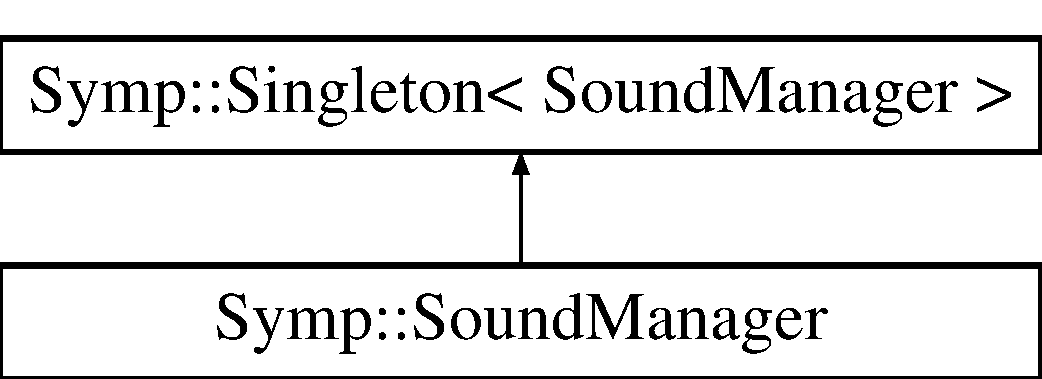
\includegraphics[height=2.000000cm]{class_symp_1_1_sound_manager}
\end{center}
\end{figure}
\subsection*{Public Member Functions}
\begin{DoxyCompactItemize}
\item 
void \hyperlink{class_symp_1_1_sound_manager_a972352cbe24f1c8b0d7565947bb7a57c}{load\-Sound} (const char $\ast$filename, F\-M\-O\-D\-::\-Sound $\ast$$\ast$sound)
\item 
void \hyperlink{class_symp_1_1_sound_manager_ac2468cc62d82609a0b40c0fc762e41ad}{play\-Sound} (\hyperlink{class_symp_1_1_sound_entity}{Sound\-Entity} $\ast$sound)
\item 
void \hyperlink{class_symp_1_1_sound_manager_a8c9c583fca013bd40de6727dd9e73f8f}{stop\-Sound} (\hyperlink{class_symp_1_1_sound_entity}{Sound\-Entity} $\ast$sound)
\item 
void \hyperlink{class_symp_1_1_sound_manager_af34876657adc807356d0de9afda2b3e9}{set\-Volume} (\hyperlink{class_symp_1_1_sound_entity}{Sound\-Entity} $\ast$sound, float volume)
\item 
void \hyperlink{class_symp_1_1_sound_manager_a698683e6aba812834d9a9e08cadd2587}{delete\-Sound} (\hyperlink{class_symp_1_1_sound_entity}{Sound\-Entity} $\ast$sound)
\item 
void \hyperlink{class_symp_1_1_sound_manager_af80ac26864c4c5ce194ba9a83c8c77eb}{clear\-Sound\-Array} ()
\item 
void \hyperlink{class_symp_1_1_sound_manager_a7f80b283b003d17f63e3a456f1a7c595}{loop} (\hyperlink{class_symp_1_1_sound_entity}{Sound\-Entity} $\ast$sound)
\item 
void \hyperlink{class_symp_1_1_sound_manager_a57f819ab0ef3f5afabe93f79fdedf9b7}{remove\-Loop} (\hyperlink{class_symp_1_1_sound_entity}{Sound\-Entity} $\ast$sound)
\item 
void \hyperlink{class_symp_1_1_sound_manager_a69c7f20fb91625fb90e9930bf1df5832}{toggle\-Loop} (\hyperlink{class_symp_1_1_sound_entity}{Sound\-Entity} $\ast$sound)
\item 
size\-\_\-t \hyperlink{class_symp_1_1_sound_manager_ab96e94d7739ae86a580417fc19a88037}{get\-Sounds\-Count} ()
\item 
void \hyperlink{class_symp_1_1_sound_manager_aa82b83dfbd0b594da8373304e9b414ce}{err\-Check} ()
\end{DoxyCompactItemize}
\subsection*{Friends}
\begin{DoxyCompactItemize}
\item 
class \hyperlink{class_symp_1_1_sound_manager_a0caa66cbb01357370233dc2bd5fdb585}{Singleton$<$ Sound\-Manager $>$}
\end{DoxyCompactItemize}
\subsection*{Additional Inherited Members}


\subsection{Detailed Description}
Facade of F\-M\-O\-D. \hyperlink{class_symp_1_1_sound_manager}{Sound\-Manager} class is a facade of the library F\-M\-O\-D Ex. It manages all sound effects of the game. 

Definition at line 44 of file Sound\-Manager.\-h.



\subsection{Member Function Documentation}
\hypertarget{class_symp_1_1_sound_manager_af80ac26864c4c5ce194ba9a83c8c77eb}{\index{Symp\-::\-Sound\-Manager@{Symp\-::\-Sound\-Manager}!clear\-Sound\-Array@{clear\-Sound\-Array}}
\index{clear\-Sound\-Array@{clear\-Sound\-Array}!Symp::SoundManager@{Symp\-::\-Sound\-Manager}}
\subsubsection[{clear\-Sound\-Array}]{\setlength{\rightskip}{0pt plus 5cm}void Symp\-::\-Sound\-Manager\-::clear\-Sound\-Array (
\begin{DoxyParamCaption}
{}
\end{DoxyParamCaption}
)}}\label{class_symp_1_1_sound_manager_af80ac26864c4c5ce194ba9a83c8c77eb}


Definition at line 95 of file Sound\-Manager.\-cpp.

\hypertarget{class_symp_1_1_sound_manager_a698683e6aba812834d9a9e08cadd2587}{\index{Symp\-::\-Sound\-Manager@{Symp\-::\-Sound\-Manager}!delete\-Sound@{delete\-Sound}}
\index{delete\-Sound@{delete\-Sound}!Symp::SoundManager@{Symp\-::\-Sound\-Manager}}
\subsubsection[{delete\-Sound}]{\setlength{\rightskip}{0pt plus 5cm}void Symp\-::\-Sound\-Manager\-::delete\-Sound (
\begin{DoxyParamCaption}
\item[{{\bf Sound\-Entity} $\ast$}]{sound}
\end{DoxyParamCaption}
)}}\label{class_symp_1_1_sound_manager_a698683e6aba812834d9a9e08cadd2587}


Definition at line 89 of file Sound\-Manager.\-cpp.

\hypertarget{class_symp_1_1_sound_manager_aa82b83dfbd0b594da8373304e9b414ce}{\index{Symp\-::\-Sound\-Manager@{Symp\-::\-Sound\-Manager}!err\-Check@{err\-Check}}
\index{err\-Check@{err\-Check}!Symp::SoundManager@{Symp\-::\-Sound\-Manager}}
\subsubsection[{err\-Check}]{\setlength{\rightskip}{0pt plus 5cm}void Symp\-::\-Sound\-Manager\-::err\-Check (
\begin{DoxyParamCaption}
{}
\end{DoxyParamCaption}
)\hspace{0.3cm}{\ttfamily [inline]}}}\label{class_symp_1_1_sound_manager_aa82b83dfbd0b594da8373304e9b414ce}


Definition at line 93 of file Sound\-Manager.\-h.

\hypertarget{class_symp_1_1_sound_manager_ab96e94d7739ae86a580417fc19a88037}{\index{Symp\-::\-Sound\-Manager@{Symp\-::\-Sound\-Manager}!get\-Sounds\-Count@{get\-Sounds\-Count}}
\index{get\-Sounds\-Count@{get\-Sounds\-Count}!Symp::SoundManager@{Symp\-::\-Sound\-Manager}}
\subsubsection[{get\-Sounds\-Count}]{\setlength{\rightskip}{0pt plus 5cm}size\-\_\-t Symp\-::\-Sound\-Manager\-::get\-Sounds\-Count (
\begin{DoxyParamCaption}
{}
\end{DoxyParamCaption}
)\hspace{0.3cm}{\ttfamily [inline]}}}\label{class_symp_1_1_sound_manager_ab96e94d7739ae86a580417fc19a88037}
Getters 

Definition at line 91 of file Sound\-Manager.\-h.

\hypertarget{class_symp_1_1_sound_manager_a972352cbe24f1c8b0d7565947bb7a57c}{\index{Symp\-::\-Sound\-Manager@{Symp\-::\-Sound\-Manager}!load\-Sound@{load\-Sound}}
\index{load\-Sound@{load\-Sound}!Symp::SoundManager@{Symp\-::\-Sound\-Manager}}
\subsubsection[{load\-Sound}]{\setlength{\rightskip}{0pt plus 5cm}void Symp\-::\-Sound\-Manager\-::load\-Sound (
\begin{DoxyParamCaption}
\item[{const char $\ast$}]{filename, }
\item[{F\-M\-O\-D\-::\-Sound $\ast$$\ast$}]{sound}
\end{DoxyParamCaption}
)}}\label{class_symp_1_1_sound_manager_a972352cbe24f1c8b0d7565947bb7a57c}
Load a sound from a filename 

Definition at line 59 of file Sound\-Manager.\-cpp.

\hypertarget{class_symp_1_1_sound_manager_a7f80b283b003d17f63e3a456f1a7c595}{\index{Symp\-::\-Sound\-Manager@{Symp\-::\-Sound\-Manager}!loop@{loop}}
\index{loop@{loop}!Symp::SoundManager@{Symp\-::\-Sound\-Manager}}
\subsubsection[{loop}]{\setlength{\rightskip}{0pt plus 5cm}void Symp\-::\-Sound\-Manager\-::loop (
\begin{DoxyParamCaption}
\item[{{\bf Sound\-Entity} $\ast$}]{sound}
\end{DoxyParamCaption}
)}}\label{class_symp_1_1_sound_manager_a7f80b283b003d17f63e3a456f1a7c595}
Setters 

Definition at line 99 of file Sound\-Manager.\-cpp.

\hypertarget{class_symp_1_1_sound_manager_ac2468cc62d82609a0b40c0fc762e41ad}{\index{Symp\-::\-Sound\-Manager@{Symp\-::\-Sound\-Manager}!play\-Sound@{play\-Sound}}
\index{play\-Sound@{play\-Sound}!Symp::SoundManager@{Symp\-::\-Sound\-Manager}}
\subsubsection[{play\-Sound}]{\setlength{\rightskip}{0pt plus 5cm}void Symp\-::\-Sound\-Manager\-::play\-Sound (
\begin{DoxyParamCaption}
\item[{{\bf Sound\-Entity} $\ast$}]{sound}
\end{DoxyParamCaption}
)}}\label{class_symp_1_1_sound_manager_ac2468cc62d82609a0b40c0fc762e41ad}
Play the indicated sound 

Definition at line 67 of file Sound\-Manager.\-cpp.

\hypertarget{class_symp_1_1_sound_manager_a57f819ab0ef3f5afabe93f79fdedf9b7}{\index{Symp\-::\-Sound\-Manager@{Symp\-::\-Sound\-Manager}!remove\-Loop@{remove\-Loop}}
\index{remove\-Loop@{remove\-Loop}!Symp::SoundManager@{Symp\-::\-Sound\-Manager}}
\subsubsection[{remove\-Loop}]{\setlength{\rightskip}{0pt plus 5cm}void Symp\-::\-Sound\-Manager\-::remove\-Loop (
\begin{DoxyParamCaption}
\item[{{\bf Sound\-Entity} $\ast$}]{sound}
\end{DoxyParamCaption}
)}}\label{class_symp_1_1_sound_manager_a57f819ab0ef3f5afabe93f79fdedf9b7}


Definition at line 104 of file Sound\-Manager.\-cpp.

\hypertarget{class_symp_1_1_sound_manager_af34876657adc807356d0de9afda2b3e9}{\index{Symp\-::\-Sound\-Manager@{Symp\-::\-Sound\-Manager}!set\-Volume@{set\-Volume}}
\index{set\-Volume@{set\-Volume}!Symp::SoundManager@{Symp\-::\-Sound\-Manager}}
\subsubsection[{set\-Volume}]{\setlength{\rightskip}{0pt plus 5cm}void Symp\-::\-Sound\-Manager\-::set\-Volume (
\begin{DoxyParamCaption}
\item[{{\bf Sound\-Entity} $\ast$}]{sound, }
\item[{float}]{volume}
\end{DoxyParamCaption}
)}}\label{class_symp_1_1_sound_manager_af34876657adc807356d0de9afda2b3e9}
Set the volume of the indicated sound 

Definition at line 83 of file Sound\-Manager.\-cpp.

\hypertarget{class_symp_1_1_sound_manager_a8c9c583fca013bd40de6727dd9e73f8f}{\index{Symp\-::\-Sound\-Manager@{Symp\-::\-Sound\-Manager}!stop\-Sound@{stop\-Sound}}
\index{stop\-Sound@{stop\-Sound}!Symp::SoundManager@{Symp\-::\-Sound\-Manager}}
\subsubsection[{stop\-Sound}]{\setlength{\rightskip}{0pt plus 5cm}void Symp\-::\-Sound\-Manager\-::stop\-Sound (
\begin{DoxyParamCaption}
\item[{{\bf Sound\-Entity} $\ast$}]{sound}
\end{DoxyParamCaption}
)}}\label{class_symp_1_1_sound_manager_a8c9c583fca013bd40de6727dd9e73f8f}
Stop the indicated sound 

Definition at line 74 of file Sound\-Manager.\-cpp.

\hypertarget{class_symp_1_1_sound_manager_a69c7f20fb91625fb90e9930bf1df5832}{\index{Symp\-::\-Sound\-Manager@{Symp\-::\-Sound\-Manager}!toggle\-Loop@{toggle\-Loop}}
\index{toggle\-Loop@{toggle\-Loop}!Symp::SoundManager@{Symp\-::\-Sound\-Manager}}
\subsubsection[{toggle\-Loop}]{\setlength{\rightskip}{0pt plus 5cm}void Symp\-::\-Sound\-Manager\-::toggle\-Loop (
\begin{DoxyParamCaption}
\item[{{\bf Sound\-Entity} $\ast$}]{sound}
\end{DoxyParamCaption}
)}}\label{class_symp_1_1_sound_manager_a69c7f20fb91625fb90e9930bf1df5832}


Definition at line 109 of file Sound\-Manager.\-cpp.



\subsection{Friends And Related Function Documentation}
\hypertarget{class_symp_1_1_sound_manager_a0caa66cbb01357370233dc2bd5fdb585}{\index{Symp\-::\-Sound\-Manager@{Symp\-::\-Sound\-Manager}!Singleton$<$ Sound\-Manager $>$@{Singleton$<$ Sound\-Manager $>$}}
\index{Singleton$<$ Sound\-Manager $>$@{Singleton$<$ Sound\-Manager $>$}!Symp::SoundManager@{Symp\-::\-Sound\-Manager}}
\subsubsection[{Singleton$<$ Sound\-Manager $>$}]{\setlength{\rightskip}{0pt plus 5cm}friend class {\bf Singleton}$<$ {\bf Sound\-Manager} $>$\hspace{0.3cm}{\ttfamily [friend]}}}\label{class_symp_1_1_sound_manager_a0caa66cbb01357370233dc2bd5fdb585}


Definition at line 47 of file Sound\-Manager.\-h.



The documentation for this class was generated from the following files\-:\begin{DoxyCompactItemize}
\item 
/home/cecilia/\-Documents/\-Symptogen/src/sound/\hyperlink{_sound_manager_8h}{Sound\-Manager.\-h}\item 
/home/cecilia/\-Documents/\-Symptogen/src/sound/\hyperlink{_sound_manager_8cpp}{Sound\-Manager.\-cpp}\end{DoxyCompactItemize}

\hypertarget{class_symp_1_1_state}{\section{Symp\-:\-:State Class Reference}
\label{class_symp_1_1_state}\index{Symp\-::\-State@{Symp\-::\-State}}
}


{\ttfamily \#include $<$State.\-h$>$}

Inheritance diagram for Symp\-:\-:State\-:\begin{figure}[H]
\begin{center}
\leavevmode
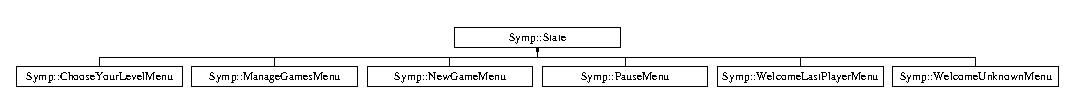
\includegraphics[height=0.933333cm]{class_symp_1_1_state}
\end{center}
\end{figure}
\subsection*{Public Member Functions}
\begin{DoxyCompactItemize}
\item 
\hyperlink{class_symp_1_1_state_ad44d90b6e1b68eb021ceaa0cb98141a4}{State} ()
\begin{DoxyCompactList}\small\item\em \hyperlink{class_symp_1_1_state}{State} class constructor Responsible for the initialization of the only class private attribute. \end{DoxyCompactList}\item 
virtual \hyperlink{class_symp_1_1_state_a52aa946045142cb351fccf6c66648d75}{$\sim$\-State} ()
\begin{DoxyCompactList}\small\item\em virtual destructor \end{DoxyCompactList}\item 
virtual void \hyperlink{class_symp_1_1_state_a2c1c597b1235128a356c7529c42fdec3}{init} ()=0
\begin{DoxyCompactList}\small\item\em virtual function that initialize the graphical components of a menu \end{DoxyCompactList}\item 
virtual void \hyperlink{class_symp_1_1_state_a23e468a10d9be4c79d17e22d1d5ef478}{handle\-Mouse\-Clic} (int mouse\-X, int mouse\-Y)=0
\begin{DoxyCompactList}\small\item\em virtual function that forward the mouse clic event to the menu logic The events are retrieved by the \#\-Game\-Manager and transmitted to the game or to the menu following the current state of the application. \end{DoxyCompactList}\item 
virtual void \hyperlink{class_symp_1_1_state_ac9ff920d185cdc17c9bc3ac63b40c62d}{key\-Down\-Pressed} ()=0
\begin{DoxyCompactList}\small\item\em virtual function that forward the key down event to the menu logic The events are retrieved by the \#\-Game\-Manager and transmitted to the game or to the menu following the current state of the application. \end{DoxyCompactList}\item 
virtual void \hyperlink{class_symp_1_1_state_a67d0fc2a02808bbcfdb06935c3be404f}{key\-Up\-Pressed} ()=0
\begin{DoxyCompactList}\small\item\em virtual function that forward the key up event to the menu logic The events are retrieved by the \#\-Game\-Manager and transmitted to the game or to the menu following the current state of the application. \end{DoxyCompactList}\end{DoxyCompactItemize}


\subsection{Detailed Description}


Definition at line 15 of file State.\-h.



\subsection{Constructor \& Destructor Documentation}
\hypertarget{class_symp_1_1_state_ad44d90b6e1b68eb021ceaa0cb98141a4}{\index{Symp\-::\-State@{Symp\-::\-State}!State@{State}}
\index{State@{State}!Symp::State@{Symp\-::\-State}}
\subsubsection[{State}]{\setlength{\rightskip}{0pt plus 5cm}Symp\-::\-State\-::\-State (
\begin{DoxyParamCaption}
{}
\end{DoxyParamCaption}
)\hspace{0.3cm}{\ttfamily [inline]}}}\label{class_symp_1_1_state_ad44d90b6e1b68eb021ceaa0cb98141a4}


\hyperlink{class_symp_1_1_state}{State} class constructor Responsible for the initialization of the only class private attribute. 

\begin{DoxySeeAlso}{See Also}
\hyperlink{class_symp_1_1_state_a2c1c597b1235128a356c7529c42fdec3}{State\-::init()} 

\hyperlink{class_symp_1_1_menu_manager}{Menu\-Manager} 
\end{DoxySeeAlso}


Definition at line 23 of file State.\-h.

\hypertarget{class_symp_1_1_state_a52aa946045142cb351fccf6c66648d75}{\index{Symp\-::\-State@{Symp\-::\-State}!$\sim$\-State@{$\sim$\-State}}
\index{$\sim$\-State@{$\sim$\-State}!Symp::State@{Symp\-::\-State}}
\subsubsection[{$\sim$\-State}]{\setlength{\rightskip}{0pt plus 5cm}virtual Symp\-::\-State\-::$\sim$\-State (
\begin{DoxyParamCaption}
{}
\end{DoxyParamCaption}
)\hspace{0.3cm}{\ttfamily [inline]}, {\ttfamily [virtual]}}}\label{class_symp_1_1_state_a52aa946045142cb351fccf6c66648d75}


virtual destructor 

\begin{DoxySeeAlso}{See Also}
\hyperlink{class_symp_1_1_state}{State} 

\hyperlink{class_symp_1_1_menu_manager}{Menu\-Manager} 
\end{DoxySeeAlso}


Definition at line 29 of file State.\-h.



\subsection{Member Function Documentation}
\hypertarget{class_symp_1_1_state_a23e468a10d9be4c79d17e22d1d5ef478}{\index{Symp\-::\-State@{Symp\-::\-State}!handle\-Mouse\-Clic@{handle\-Mouse\-Clic}}
\index{handle\-Mouse\-Clic@{handle\-Mouse\-Clic}!Symp::State@{Symp\-::\-State}}
\subsubsection[{handle\-Mouse\-Clic}]{\setlength{\rightskip}{0pt plus 5cm}virtual void Symp\-::\-State\-::handle\-Mouse\-Clic (
\begin{DoxyParamCaption}
\item[{int}]{mouse\-X, }
\item[{int}]{mouse\-Y}
\end{DoxyParamCaption}
)\hspace{0.3cm}{\ttfamily [pure virtual]}}}\label{class_symp_1_1_state_a23e468a10d9be4c79d17e22d1d5ef478}


virtual function that forward the mouse clic event to the menu logic The events are retrieved by the \#\-Game\-Manager and transmitted to the game or to the menu following the current state of the application. 


\begin{DoxyParams}{Parameters}
{\em mouse\-X} & the x coordinate of the mouse clic position \\
\hline
{\em mouse\-Y} & the y coordinate of the mouse clic position \\
\hline
\end{DoxyParams}
\begin{DoxySeeAlso}{See Also}
\hyperlink{class_symp_1_1_state}{State} 

\hyperlink{class_symp_1_1_menu_manager}{Menu\-Manager} 

\hyperlink{class_symp_1_1_game_manager_a53eae391ee3ea958e26d60b51516c770}{Game\-Manager\-::update\-Menu()} 
\end{DoxySeeAlso}


Implemented in \hyperlink{class_symp_1_1_manage_games_menu_acbca4c010ddb4a39fcdc1b0e3716bb03}{Symp\-::\-Manage\-Games\-Menu}, \hyperlink{class_symp_1_1_welcome_last_player_menu_a372720625563d47b3814c40f836ecc14}{Symp\-::\-Welcome\-Last\-Player\-Menu}, \hyperlink{class_symp_1_1_choose_your_level_menu_a8c3ad10284b68e12df75ff980a7fc657}{Symp\-::\-Choose\-Your\-Level\-Menu}, \hyperlink{class_symp_1_1_new_game_menu_a2e02c1b26f7e221de7a4cae2e856a41c}{Symp\-::\-New\-Game\-Menu}, \hyperlink{class_symp_1_1_welcome_unknown_menu_aab730d45332061d9028802a34bf307a4}{Symp\-::\-Welcome\-Unknown\-Menu}, and \hyperlink{class_symp_1_1_pause_menu_a2a4fd25c988e7b2db561af0f76449cda}{Symp\-::\-Pause\-Menu}.

\hypertarget{class_symp_1_1_state_a2c1c597b1235128a356c7529c42fdec3}{\index{Symp\-::\-State@{Symp\-::\-State}!init@{init}}
\index{init@{init}!Symp::State@{Symp\-::\-State}}
\subsubsection[{init}]{\setlength{\rightskip}{0pt plus 5cm}virtual void Symp\-::\-State\-::init (
\begin{DoxyParamCaption}
{}
\end{DoxyParamCaption}
)\hspace{0.3cm}{\ttfamily [pure virtual]}}}\label{class_symp_1_1_state_a2c1c597b1235128a356c7529c42fdec3}


virtual function that initialize the graphical components of a menu 

\begin{DoxySeeAlso}{See Also}
\hyperlink{class_symp_1_1_state}{State} 

\hyperlink{class_symp_1_1_menu_manager}{Menu\-Manager} 
\end{DoxySeeAlso}


Implemented in \hyperlink{class_symp_1_1_manage_games_menu_a2cac1836c3c7272633a99beb0287f9b1}{Symp\-::\-Manage\-Games\-Menu}, \hyperlink{class_symp_1_1_welcome_last_player_menu_a04a8fb21c22309adc020fd074ede1ffc}{Symp\-::\-Welcome\-Last\-Player\-Menu}, \hyperlink{class_symp_1_1_choose_your_level_menu_a18c2d2aec31b070ecdd5ec8d2c8b4cbf}{Symp\-::\-Choose\-Your\-Level\-Menu}, \hyperlink{class_symp_1_1_new_game_menu_a8f57888361e8424acedda26143fd7746}{Symp\-::\-New\-Game\-Menu}, \hyperlink{class_symp_1_1_welcome_unknown_menu_a57182187076a7158a71ad395bfdc1202}{Symp\-::\-Welcome\-Unknown\-Menu}, and \hyperlink{class_symp_1_1_pause_menu_af456bb275fc71d5a9ee3290e5d82cd90}{Symp\-::\-Pause\-Menu}.

\hypertarget{class_symp_1_1_state_ac9ff920d185cdc17c9bc3ac63b40c62d}{\index{Symp\-::\-State@{Symp\-::\-State}!key\-Down\-Pressed@{key\-Down\-Pressed}}
\index{key\-Down\-Pressed@{key\-Down\-Pressed}!Symp::State@{Symp\-::\-State}}
\subsubsection[{key\-Down\-Pressed}]{\setlength{\rightskip}{0pt plus 5cm}virtual void Symp\-::\-State\-::key\-Down\-Pressed (
\begin{DoxyParamCaption}
{}
\end{DoxyParamCaption}
)\hspace{0.3cm}{\ttfamily [pure virtual]}}}\label{class_symp_1_1_state_ac9ff920d185cdc17c9bc3ac63b40c62d}


virtual function that forward the key down event to the menu logic The events are retrieved by the \#\-Game\-Manager and transmitted to the game or to the menu following the current state of the application. 

\begin{DoxySeeAlso}{See Also}
\hyperlink{class_symp_1_1_state}{State} 

\hyperlink{class_symp_1_1_menu_manager}{Menu\-Manager} 

\hyperlink{class_symp_1_1_game_manager_a53eae391ee3ea958e26d60b51516c770}{Game\-Manager\-::update\-Menu()} 
\end{DoxySeeAlso}


Implemented in \hyperlink{class_symp_1_1_manage_games_menu_ab330c9d8b0103d7232dc698e01d8e820}{Symp\-::\-Manage\-Games\-Menu}, \hyperlink{class_symp_1_1_welcome_last_player_menu_aa275509ff5be0d17303c7a0bccc6d9fd}{Symp\-::\-Welcome\-Last\-Player\-Menu}, \hyperlink{class_symp_1_1_choose_your_level_menu_a2a66e7d44ceca790b987eca33fa478ff}{Symp\-::\-Choose\-Your\-Level\-Menu}, \hyperlink{class_symp_1_1_new_game_menu_a4c52d19b89c3122ca989c2149467cdd2}{Symp\-::\-New\-Game\-Menu}, \hyperlink{class_symp_1_1_welcome_unknown_menu_a6d4dcd79840d2ae8b0ad17759c3ffdac}{Symp\-::\-Welcome\-Unknown\-Menu}, and \hyperlink{class_symp_1_1_pause_menu_af20fcbac9585f1e34eef8de5c84bf9e3}{Symp\-::\-Pause\-Menu}.

\hypertarget{class_symp_1_1_state_a67d0fc2a02808bbcfdb06935c3be404f}{\index{Symp\-::\-State@{Symp\-::\-State}!key\-Up\-Pressed@{key\-Up\-Pressed}}
\index{key\-Up\-Pressed@{key\-Up\-Pressed}!Symp::State@{Symp\-::\-State}}
\subsubsection[{key\-Up\-Pressed}]{\setlength{\rightskip}{0pt plus 5cm}virtual void Symp\-::\-State\-::key\-Up\-Pressed (
\begin{DoxyParamCaption}
{}
\end{DoxyParamCaption}
)\hspace{0.3cm}{\ttfamily [pure virtual]}}}\label{class_symp_1_1_state_a67d0fc2a02808bbcfdb06935c3be404f}


virtual function that forward the key up event to the menu logic The events are retrieved by the \#\-Game\-Manager and transmitted to the game or to the menu following the current state of the application. 

\begin{DoxySeeAlso}{See Also}
\hyperlink{class_symp_1_1_state}{State} 

\hyperlink{class_symp_1_1_menu_manager}{Menu\-Manager} 

\hyperlink{class_symp_1_1_game_manager_a53eae391ee3ea958e26d60b51516c770}{Game\-Manager\-::update\-Menu()} 
\end{DoxySeeAlso}


Implemented in \hyperlink{class_symp_1_1_manage_games_menu_a31141c164d9d36c51eb1a0b5803f0974}{Symp\-::\-Manage\-Games\-Menu}, \hyperlink{class_symp_1_1_welcome_last_player_menu_ab277e548cec10d96524643b117831a52}{Symp\-::\-Welcome\-Last\-Player\-Menu}, \hyperlink{class_symp_1_1_choose_your_level_menu_a59974b0d10b806ed646569b4b658d68f}{Symp\-::\-Choose\-Your\-Level\-Menu}, \hyperlink{class_symp_1_1_new_game_menu_abb3d59240c9874026dd996bc9fb9a290}{Symp\-::\-New\-Game\-Menu}, \hyperlink{class_symp_1_1_welcome_unknown_menu_a2fcfb802e8398d1a5178b904841650fb}{Symp\-::\-Welcome\-Unknown\-Menu}, and \hyperlink{class_symp_1_1_pause_menu_ab6329d721b22dfb991e794768e0d5afd}{Symp\-::\-Pause\-Menu}.



The documentation for this class was generated from the following file\-:\begin{DoxyCompactItemize}
\item 
/home/cecilia/\-Documents/\-Symptogen/src/menu/\hyperlink{_state_8h}{State.\-h}\end{DoxyCompactItemize}

\hypertarget{class_symp_1_1_text}{\section{Symp\-:\-:Text Class Reference}
\label{class_symp_1_1_text}\index{Symp\-::\-Text@{Symp\-::\-Text}}
}


\hyperlink{class_symp_1_1_text}{Text} class. This class inherits the \hyperlink{class_symp_1_1_gui_component_a22124675c2976983ac18374f81cc3fb3}{Gui\-Component} class.  




{\ttfamily \#include $<$Text.\-h$>$}

Inheritance diagram for Symp\-:\-:Text\-:\begin{figure}[H]
\begin{center}
\leavevmode
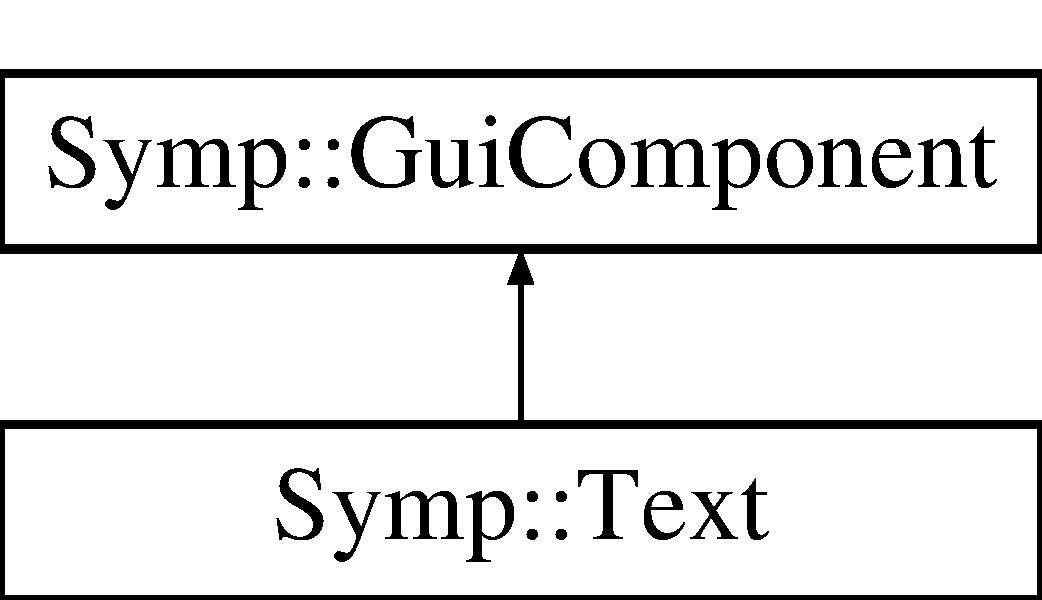
\includegraphics[height=2.000000cm]{class_symp_1_1_text}
\end{center}
\end{figure}
\subsection*{Public Member Functions}
\begin{DoxyCompactItemize}
\item 
\hyperlink{class_symp_1_1_text_aa873244778f3aed01a7d7ecd9ce7006c}{Text} (std\-::string text, \hyperlink{struct_symp_1_1_color}{Symp\-::\-Color} color=\hyperlink{struct_symp_1_1_color}{Color}(0, 0, 0), float i\-Pos\-X=0, float i\-Pos\-Y=0, bool b\-\_\-small\-Font=false)
\begin{DoxyCompactList}\small\item\em \hyperlink{class_symp_1_1_text}{Text} class constructor inherits the \hyperlink{class_symp_1_1_gui_component}{Gui\-Component} class Responsible for the initialization of the only class private attribute. \end{DoxyCompactList}\item 
\hyperlink{class_symp_1_1_text_aa960cbce42553cab1c0e8118da966671}{$\sim$\-Text} ()
\item 
virtual void \hyperlink{class_symp_1_1_text_ab11eff488943981a0009549b77249a46}{update} ()
\begin{DoxyCompactList}\small\item\em \hyperlink{class_symp_1_1_text}{Text} update fonction Refresh the display of the \hyperlink{class_symp_1_1_text_aa873244778f3aed01a7d7ecd9ce7006c}{Text}. \end{DoxyCompactList}\item 
void \hyperlink{class_symp_1_1_text_a95198e44aa23b2948f844c1485b74f6f}{fill} (\hyperlink{struct_symp_1_1_color}{Symp\-::\-Color} color)
\begin{DoxyCompactList}\small\item\em fill \hyperlink{class_symp_1_1_text}{Text}'s background function \end{DoxyCompactList}\item 
void \hyperlink{class_symp_1_1_text_adcc35d491c41815f9cd1a5dd4d5b5a2c}{center\-X} (int y\-Pos)
\begin{DoxyCompactList}\small\item\em Center the \hyperlink{class_symp_1_1_text}{Text} in the x axis Refresh the display of the \hyperlink{class_symp_1_1_text_aa873244778f3aed01a7d7ecd9ce7006c}{Text}. \end{DoxyCompactList}\item 
void \hyperlink{class_symp_1_1_text_a0ab23dd09b189a4b61704a910273dcaa}{center\-Y} (int x\-Pos)
\begin{DoxyCompactList}\small\item\em Center the \hyperlink{class_symp_1_1_text}{Text} in the y axis Refresh the display of the \hyperlink{class_symp_1_1_text_aa873244778f3aed01a7d7ecd9ce7006c}{Text}. \end{DoxyCompactList}\item 
std\-::string \hyperlink{class_symp_1_1_text_a53b5852173ebf3093e857faddee74908}{get\-Text} () const 
\item 
void \hyperlink{class_symp_1_1_text_a9f3145a0f73eba8b65e4bfe8cb14d4c1}{set\-Text} (std\-::string text)
\end{DoxyCompactItemize}
\subsection*{Additional Inherited Members}


\subsection{Detailed Description}
\hyperlink{class_symp_1_1_text}{Text} class. This class inherits the \hyperlink{class_symp_1_1_gui_component_a22124675c2976983ac18374f81cc3fb3}{Gui\-Component} class. 

\begin{DoxySeeAlso}{See Also}
\hyperlink{class_symp_1_1_menu_manager}{Menu\-Manager} 

\hyperlink{class_symp_1_1_text}{Text} 

\hyperlink{class_symp_1_1_gui_component}{Gui\-Component} 

\hyperlink{class_symp_1_1_layout}{Layout} 
\end{DoxySeeAlso}


Definition at line 17 of file Text.\-h.



\subsection{Constructor \& Destructor Documentation}
\hypertarget{class_symp_1_1_text_aa873244778f3aed01a7d7ecd9ce7006c}{\index{Symp\-::\-Text@{Symp\-::\-Text}!Text@{Text}}
\index{Text@{Text}!Symp::Text@{Symp\-::\-Text}}
\subsubsection[{Text}]{\setlength{\rightskip}{0pt plus 5cm}Symp\-::\-Text\-::\-Text (
\begin{DoxyParamCaption}
\item[{std\-::string}]{text, }
\item[{{\bf Symp\-::\-Color}}]{color = {\ttfamily {\bf Color}(0,0,0)}, }
\item[{float}]{i\-Pos\-X = {\ttfamily 0}, }
\item[{float}]{i\-Pos\-Y = {\ttfamily 0}, }
\item[{bool}]{b\-\_\-small\-Font = {\ttfamily false}}
\end{DoxyParamCaption}
)}}\label{class_symp_1_1_text_aa873244778f3aed01a7d7ecd9ce7006c}


\hyperlink{class_symp_1_1_text}{Text} class constructor inherits the \hyperlink{class_symp_1_1_gui_component}{Gui\-Component} class Responsible for the initialization of the only class private attribute. 


\begin{DoxyParams}{Parameters}
{\em text} & is the text that will be displayed by the \hyperlink{class_symp_1_1_text_aa873244778f3aed01a7d7ecd9ce7006c}{Text} \\
\hline
{\em color} & is the color that will fill the \hyperlink{class_symp_1_1_text_aa873244778f3aed01a7d7ecd9ce7006c}{Text} following the \#i\-Weight attributes \\
\hline
\end{DoxyParams}
\begin{DoxySeeAlso}{See Also}
\hyperlink{class_symp_1_1_text}{Text} 

\hyperlink{class_symp_1_1_text_aa960cbce42553cab1c0e8118da966671}{$\sim$\-Text()} 

\hyperlink{struct_symp_1_1_color}{Color} 

\hyperlink{class_symp_1_1_layout}{Layout} 

\hyperlink{class_symp_1_1_gui_component}{Gui\-Component} 
\end{DoxySeeAlso}


Definition at line 20 of file Text.\-cpp.

\hypertarget{class_symp_1_1_text_aa960cbce42553cab1c0e8118da966671}{\index{Symp\-::\-Text@{Symp\-::\-Text}!$\sim$\-Text@{$\sim$\-Text}}
\index{$\sim$\-Text@{$\sim$\-Text}!Symp::Text@{Symp\-::\-Text}}
\subsubsection[{$\sim$\-Text}]{\setlength{\rightskip}{0pt plus 5cm}Symp\-::\-Text\-::$\sim$\-Text (
\begin{DoxyParamCaption}
{}
\end{DoxyParamCaption}
)\hspace{0.3cm}{\ttfamily [inline]}}}\label{class_symp_1_1_text_aa960cbce42553cab1c0e8118da966671}


Definition at line 20 of file Text.\-h.



\subsection{Member Function Documentation}
\hypertarget{class_symp_1_1_text_adcc35d491c41815f9cd1a5dd4d5b5a2c}{\index{Symp\-::\-Text@{Symp\-::\-Text}!center\-X@{center\-X}}
\index{center\-X@{center\-X}!Symp::Text@{Symp\-::\-Text}}
\subsubsection[{center\-X}]{\setlength{\rightskip}{0pt plus 5cm}void Symp\-::\-Text\-::center\-X (
\begin{DoxyParamCaption}
\item[{int}]{y\-Pos}
\end{DoxyParamCaption}
)}}\label{class_symp_1_1_text_adcc35d491c41815f9cd1a5dd4d5b5a2c}


Center the \hyperlink{class_symp_1_1_text}{Text} in the x axis Refresh the display of the \hyperlink{class_symp_1_1_text_aa873244778f3aed01a7d7ecd9ce7006c}{Text}. 


\begin{DoxyParams}{Parameters}
{\em y\-Pos} & the y position of the text \\
\hline
\end{DoxyParams}
\begin{DoxySeeAlso}{See Also}
\hyperlink{class_symp_1_1_text}{Text} 

\hyperlink{class_symp_1_1_text_aa960cbce42553cab1c0e8118da966671}{$\sim$\-Text()} 

\hyperlink{class_symp_1_1_gui_component}{Gui\-Component} 
\end{DoxySeeAlso}


Definition at line 81 of file Text.\-cpp.

\hypertarget{class_symp_1_1_text_a0ab23dd09b189a4b61704a910273dcaa}{\index{Symp\-::\-Text@{Symp\-::\-Text}!center\-Y@{center\-Y}}
\index{center\-Y@{center\-Y}!Symp::Text@{Symp\-::\-Text}}
\subsubsection[{center\-Y}]{\setlength{\rightskip}{0pt plus 5cm}void Symp\-::\-Text\-::center\-Y (
\begin{DoxyParamCaption}
\item[{int}]{x\-Pos}
\end{DoxyParamCaption}
)}}\label{class_symp_1_1_text_a0ab23dd09b189a4b61704a910273dcaa}


Center the \hyperlink{class_symp_1_1_text}{Text} in the y axis Refresh the display of the \hyperlink{class_symp_1_1_text_aa873244778f3aed01a7d7ecd9ce7006c}{Text}. 


\begin{DoxyParams}{Parameters}
{\em x\-Pos} & the x position of the text \\
\hline
\end{DoxyParams}
\begin{DoxySeeAlso}{See Also}
\hyperlink{class_symp_1_1_text}{Text} 

\hyperlink{class_symp_1_1_text_aa960cbce42553cab1c0e8118da966671}{$\sim$\-Text()} 

\hyperlink{class_symp_1_1_gui_component}{Gui\-Component} 
\end{DoxySeeAlso}


Definition at line 94 of file Text.\-cpp.

\hypertarget{class_symp_1_1_text_a95198e44aa23b2948f844c1485b74f6f}{\index{Symp\-::\-Text@{Symp\-::\-Text}!fill@{fill}}
\index{fill@{fill}!Symp::Text@{Symp\-::\-Text}}
\subsubsection[{fill}]{\setlength{\rightskip}{0pt plus 5cm}void Symp\-::\-Text\-::fill (
\begin{DoxyParamCaption}
\item[{{\bf Symp\-::\-Color}}]{color}
\end{DoxyParamCaption}
)}}\label{class_symp_1_1_text_a95198e44aa23b2948f844c1485b74f6f}


fill \hyperlink{class_symp_1_1_text}{Text}'s background function 

\begin{DoxySeeAlso}{See Also}
\hyperlink{class_symp_1_1_text}{Text} 

\hyperlink{class_symp_1_1_text_aa960cbce42553cab1c0e8118da966671}{$\sim$\-Text()} 

\hyperlink{struct_symp_1_1_color}{Color} 

\hyperlink{class_symp_1_1_gui_component}{Gui\-Component} 
\end{DoxySeeAlso}


Definition at line 106 of file Text.\-cpp.

\hypertarget{class_symp_1_1_text_a53b5852173ebf3093e857faddee74908}{\index{Symp\-::\-Text@{Symp\-::\-Text}!get\-Text@{get\-Text}}
\index{get\-Text@{get\-Text}!Symp::Text@{Symp\-::\-Text}}
\subsubsection[{get\-Text}]{\setlength{\rightskip}{0pt plus 5cm}std\-::string Symp\-::\-Text\-::get\-Text (
\begin{DoxyParamCaption}
{}
\end{DoxyParamCaption}
) const\hspace{0.3cm}{\ttfamily [inline]}}}\label{class_symp_1_1_text_a53b5852173ebf3093e857faddee74908}


Definition at line 29 of file Text.\-h.

\hypertarget{class_symp_1_1_text_a9f3145a0f73eba8b65e4bfe8cb14d4c1}{\index{Symp\-::\-Text@{Symp\-::\-Text}!set\-Text@{set\-Text}}
\index{set\-Text@{set\-Text}!Symp::Text@{Symp\-::\-Text}}
\subsubsection[{set\-Text}]{\setlength{\rightskip}{0pt plus 5cm}void Symp\-::\-Text\-::set\-Text (
\begin{DoxyParamCaption}
\item[{std\-::string}]{text}
\end{DoxyParamCaption}
)\hspace{0.3cm}{\ttfamily [inline]}}}\label{class_symp_1_1_text_a9f3145a0f73eba8b65e4bfe8cb14d4c1}


Definition at line 30 of file Text.\-h.

\hypertarget{class_symp_1_1_text_ab11eff488943981a0009549b77249a46}{\index{Symp\-::\-Text@{Symp\-::\-Text}!update@{update}}
\index{update@{update}!Symp::Text@{Symp\-::\-Text}}
\subsubsection[{update}]{\setlength{\rightskip}{0pt plus 5cm}void Symp\-::\-Text\-::update (
\begin{DoxyParamCaption}
{}
\end{DoxyParamCaption}
)\hspace{0.3cm}{\ttfamily [virtual]}}}\label{class_symp_1_1_text_ab11eff488943981a0009549b77249a46}


\hyperlink{class_symp_1_1_text}{Text} update fonction Refresh the display of the \hyperlink{class_symp_1_1_text_aa873244778f3aed01a7d7ecd9ce7006c}{Text}. 

\begin{DoxySeeAlso}{See Also}
\hyperlink{class_symp_1_1_text}{Text} 

\hyperlink{class_symp_1_1_text_aa960cbce42553cab1c0e8118da966671}{$\sim$\-Text()} 

\hyperlink{class_symp_1_1_gui_component}{Gui\-Component} 
\end{DoxySeeAlso}


Implements \hyperlink{class_symp_1_1_gui_component_add73e07ea0a3c9c1c90640e783a3b5de}{Symp\-::\-Gui\-Component}.



Definition at line 51 of file Text.\-cpp.



The documentation for this class was generated from the following files\-:\begin{DoxyCompactItemize}
\item 
/home/cecilia/\-Documents/\-Symptogen/src/menu/\hyperlink{_text_8h}{Text.\-h}\item 
/home/cecilia/\-Documents/\-Symptogen/src/menu/\hyperlink{_text_8cpp}{Text.\-cpp}\end{DoxyCompactItemize}

\hypertarget{class_symp_1_1_welcome_last_player_menu}{\section{Symp\-:\-:Welcome\-Last\-Player\-Menu Class Reference}
\label{class_symp_1_1_welcome_last_player_menu}\index{Symp\-::\-Welcome\-Last\-Player\-Menu@{Symp\-::\-Welcome\-Last\-Player\-Menu}}
}


{\ttfamily \#include $<$Welcome\-Last\-Player\-Menu.\-h$>$}

Inheritance diagram for Symp\-:\-:Welcome\-Last\-Player\-Menu\-:\begin{figure}[H]
\begin{center}
\leavevmode
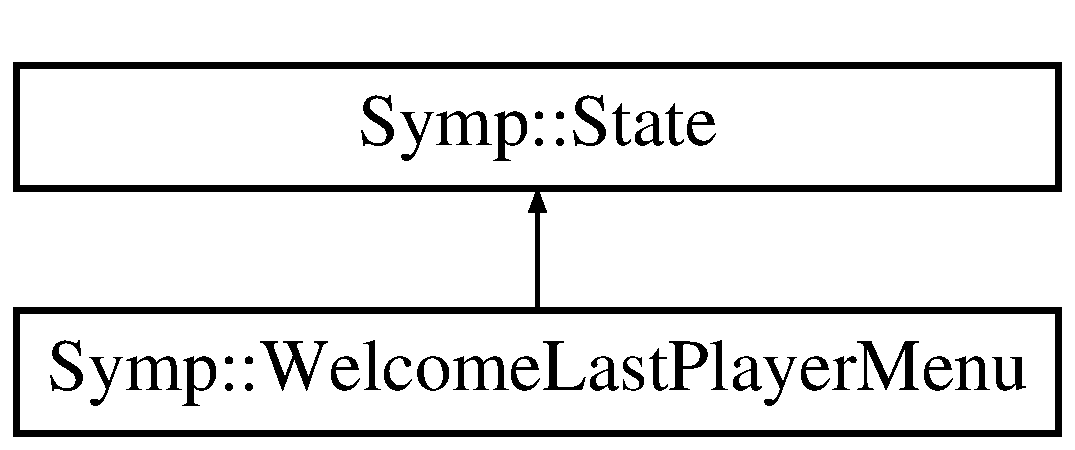
\includegraphics[height=2.000000cm]{class_symp_1_1_welcome_last_player_menu}
\end{center}
\end{figure}
\subsection*{Public Member Functions}
\begin{DoxyCompactItemize}
\item 
\hyperlink{class_symp_1_1_welcome_last_player_menu_a91f706b9f566d790ff750340b3f9761e}{Welcome\-Last\-Player\-Menu} (\hyperlink{class_symp_1_1_player}{Player} $\ast$last\-Player)
\begin{DoxyCompactList}\small\item\em \hyperlink{class_symp_1_1_welcome_last_player_menu}{Welcome\-Last\-Player\-Menu} constructor Responsible for the initialization of the private attributes of the \hyperlink{class_symp_1_1_welcome_last_player_menu_a91f706b9f566d790ff750340b3f9761e}{Welcome\-Last\-Player\-Menu} class. This function is not responsible for drawing the graphical elements that compose the menu, the \hyperlink{class_symp_1_1_welcome_last_player_menu_a04a8fb21c22309adc020fd074ede1ffc}{init()} function is. \end{DoxyCompactList}\item 
\hyperlink{class_symp_1_1_welcome_last_player_menu_a1acdc429a82e38f08dd80c22e7fef2ae}{$\sim$\-Welcome\-Last\-Player\-Menu} ()
\item 
virtual void \hyperlink{class_symp_1_1_welcome_last_player_menu_a04a8fb21c22309adc020fd074ede1ffc}{init} ()
\begin{DoxyCompactList}\small\item\em \hyperlink{class_symp_1_1_welcome_last_player_menu}{Welcome\-Last\-Player\-Menu} elements initialization The elements that compose the menu are created in this function. \end{DoxyCompactList}\item 
virtual void \hyperlink{class_symp_1_1_welcome_last_player_menu_a372720625563d47b3814c40f836ecc14}{handle\-Mouse\-Clic} (int mouse\-X, int mouse\-Y)
\begin{DoxyCompactList}\small\item\em Handle mouse clic events. \end{DoxyCompactList}\item 
virtual void \hyperlink{class_symp_1_1_welcome_last_player_menu_aa275509ff5be0d17303c7a0bccc6d9fd}{key\-Down\-Pressed} ()
\begin{DoxyCompactList}\small\item\em Handle key down event. \end{DoxyCompactList}\item 
virtual void \hyperlink{class_symp_1_1_welcome_last_player_menu_ab277e548cec10d96524643b117831a52}{key\-Up\-Pressed} ()
\begin{DoxyCompactList}\small\item\em Handle key up event. \end{DoxyCompactList}\item 
\hyperlink{class_symp_1_1_player}{Player} $\ast$ \hyperlink{class_symp_1_1_welcome_last_player_menu_a6913f956df8bb265ac01a587202a676d}{get\-Last\-Player} () const 
\end{DoxyCompactItemize}


\subsection{Detailed Description}
the \hyperlink{class_symp_1_1_state_ad44d90b6e1b68eb021ceaa0cb98141a4}{State} interface for implementing the \hyperlink{class_symp_1_1_state}{State} Machine Pattern This Menu is the first menu of the application in case players data have been found in the resources. The last known \#\-Player have a direct button for going back into its game. Otherwise, the user can go to the \#\-Manage\-Games\-Menu or quit the application. \begin{DoxySeeAlso}{See Also}
\hyperlink{class_symp_1_1_state}{State} 

\hyperlink{class_symp_1_1_player}{Player} 

\hyperlink{class_symp_1_1_game_manager}{Game\-Manager} 

\hyperlink{class_symp_1_1_manage_games_menu}{Manage\-Games\-Menu} 

\hyperlink{class_symp_1_1_menu_manager}{Menu\-Manager} 
\end{DoxySeeAlso}


Definition at line 21 of file Welcome\-Last\-Player\-Menu.\-h.



\subsection{Constructor \& Destructor Documentation}
\hypertarget{class_symp_1_1_welcome_last_player_menu_a91f706b9f566d790ff750340b3f9761e}{\index{Symp\-::\-Welcome\-Last\-Player\-Menu@{Symp\-::\-Welcome\-Last\-Player\-Menu}!Welcome\-Last\-Player\-Menu@{Welcome\-Last\-Player\-Menu}}
\index{Welcome\-Last\-Player\-Menu@{Welcome\-Last\-Player\-Menu}!Symp::WelcomeLastPlayerMenu@{Symp\-::\-Welcome\-Last\-Player\-Menu}}
\subsubsection[{Welcome\-Last\-Player\-Menu}]{\setlength{\rightskip}{0pt plus 5cm}Symp\-::\-Welcome\-Last\-Player\-Menu\-::\-Welcome\-Last\-Player\-Menu (
\begin{DoxyParamCaption}
\item[{{\bf Player} $\ast$}]{p\-Last\-Player}
\end{DoxyParamCaption}
)}}\label{class_symp_1_1_welcome_last_player_menu_a91f706b9f566d790ff750340b3f9761e}


\hyperlink{class_symp_1_1_welcome_last_player_menu}{Welcome\-Last\-Player\-Menu} constructor Responsible for the initialization of the private attributes of the \hyperlink{class_symp_1_1_welcome_last_player_menu_a91f706b9f566d790ff750340b3f9761e}{Welcome\-Last\-Player\-Menu} class. This function is not responsible for drawing the graphical elements that compose the menu, the \hyperlink{class_symp_1_1_welcome_last_player_menu_a04a8fb21c22309adc020fd074ede1ffc}{init()} function is. 


\begin{DoxyParams}{Parameters}
{\em p\-Last\-Player} & the reference to the last known \#\-Player \\
\hline
\end{DoxyParams}
\begin{DoxySeeAlso}{See Also}
\hyperlink{class_symp_1_1_player}{Player} 

\hyperlink{class_symp_1_1_menu_manager}{Menu\-Manager} 

\hyperlink{class_symp_1_1_state}{State} 

\hyperlink{class_symp_1_1_welcome_last_player_menu_a04a8fb21c22309adc020fd074ede1ffc}{init()} 

\hyperlink{class_symp_1_1_welcome_last_player_menu_a1acdc429a82e38f08dd80c22e7fef2ae}{$\sim$\-Welcome\-Last\-Player\-Menu()} 
\end{DoxySeeAlso}


Definition at line 25 of file Welcome\-Last\-Player\-Menu.\-cpp.

\hypertarget{class_symp_1_1_welcome_last_player_menu_a1acdc429a82e38f08dd80c22e7fef2ae}{\index{Symp\-::\-Welcome\-Last\-Player\-Menu@{Symp\-::\-Welcome\-Last\-Player\-Menu}!$\sim$\-Welcome\-Last\-Player\-Menu@{$\sim$\-Welcome\-Last\-Player\-Menu}}
\index{$\sim$\-Welcome\-Last\-Player\-Menu@{$\sim$\-Welcome\-Last\-Player\-Menu}!Symp::WelcomeLastPlayerMenu@{Symp\-::\-Welcome\-Last\-Player\-Menu}}
\subsubsection[{$\sim$\-Welcome\-Last\-Player\-Menu}]{\setlength{\rightskip}{0pt plus 5cm}Symp\-::\-Welcome\-Last\-Player\-Menu\-::$\sim$\-Welcome\-Last\-Player\-Menu (
\begin{DoxyParamCaption}
{}
\end{DoxyParamCaption}
)\hspace{0.3cm}{\ttfamily [inline]}}}\label{class_symp_1_1_welcome_last_player_menu_a1acdc429a82e38f08dd80c22e7fef2ae}


Definition at line 24 of file Welcome\-Last\-Player\-Menu.\-h.



\subsection{Member Function Documentation}
\hypertarget{class_symp_1_1_welcome_last_player_menu_a6913f956df8bb265ac01a587202a676d}{\index{Symp\-::\-Welcome\-Last\-Player\-Menu@{Symp\-::\-Welcome\-Last\-Player\-Menu}!get\-Last\-Player@{get\-Last\-Player}}
\index{get\-Last\-Player@{get\-Last\-Player}!Symp::WelcomeLastPlayerMenu@{Symp\-::\-Welcome\-Last\-Player\-Menu}}
\subsubsection[{get\-Last\-Player}]{\setlength{\rightskip}{0pt plus 5cm}{\bf Player}$\ast$ Symp\-::\-Welcome\-Last\-Player\-Menu\-::get\-Last\-Player (
\begin{DoxyParamCaption}
{}
\end{DoxyParamCaption}
) const\hspace{0.3cm}{\ttfamily [inline]}}}\label{class_symp_1_1_welcome_last_player_menu_a6913f956df8bb265ac01a587202a676d}


Definition at line 32 of file Welcome\-Last\-Player\-Menu.\-h.

\hypertarget{class_symp_1_1_welcome_last_player_menu_a372720625563d47b3814c40f836ecc14}{\index{Symp\-::\-Welcome\-Last\-Player\-Menu@{Symp\-::\-Welcome\-Last\-Player\-Menu}!handle\-Mouse\-Clic@{handle\-Mouse\-Clic}}
\index{handle\-Mouse\-Clic@{handle\-Mouse\-Clic}!Symp::WelcomeLastPlayerMenu@{Symp\-::\-Welcome\-Last\-Player\-Menu}}
\subsubsection[{handle\-Mouse\-Clic}]{\setlength{\rightskip}{0pt plus 5cm}void Symp\-::\-Welcome\-Last\-Player\-Menu\-::handle\-Mouse\-Clic (
\begin{DoxyParamCaption}
\item[{int}]{mouse\-X, }
\item[{int}]{mouse\-Y}
\end{DoxyParamCaption}
)\hspace{0.3cm}{\ttfamily [virtual]}}}\label{class_symp_1_1_welcome_last_player_menu_a372720625563d47b3814c40f836ecc14}


Handle mouse clic events. 


\begin{DoxyParams}{Parameters}
{\em mouse\-X} & the x coordinate of the mouse position \\
\hline
{\em mouse\-Y} & the y coordinate of the mouse position \\
\hline
\end{DoxyParams}
\begin{DoxySeeAlso}{See Also}
\hyperlink{class_symp_1_1_menu_manager}{Menu\-Manager} 

\hyperlink{class_symp_1_1_state}{State} 

\hyperlink{class_symp_1_1_input_manager}{Input\-Manager} 

\hyperlink{class_symp_1_1_welcome_last_player_menu_a04a8fb21c22309adc020fd074ede1ffc}{init()} 
\end{DoxySeeAlso}


Implements \hyperlink{class_symp_1_1_state_a23e468a10d9be4c79d17e22d1d5ef478}{Symp\-::\-State}.



Definition at line 94 of file Welcome\-Last\-Player\-Menu.\-cpp.

\hypertarget{class_symp_1_1_welcome_last_player_menu_a04a8fb21c22309adc020fd074ede1ffc}{\index{Symp\-::\-Welcome\-Last\-Player\-Menu@{Symp\-::\-Welcome\-Last\-Player\-Menu}!init@{init}}
\index{init@{init}!Symp::WelcomeLastPlayerMenu@{Symp\-::\-Welcome\-Last\-Player\-Menu}}
\subsubsection[{init}]{\setlength{\rightskip}{0pt plus 5cm}void Symp\-::\-Welcome\-Last\-Player\-Menu\-::init (
\begin{DoxyParamCaption}
{}
\end{DoxyParamCaption}
)\hspace{0.3cm}{\ttfamily [virtual]}}}\label{class_symp_1_1_welcome_last_player_menu_a04a8fb21c22309adc020fd074ede1ffc}


\hyperlink{class_symp_1_1_welcome_last_player_menu}{Welcome\-Last\-Player\-Menu} elements initialization The elements that compose the menu are created in this function. 

\begin{DoxySeeAlso}{See Also}
\hyperlink{class_symp_1_1_player}{Player} 

\hyperlink{class_symp_1_1_menu_manager}{Menu\-Manager} 

\hyperlink{class_symp_1_1_state}{State} 

end() 

\hyperlink{class_symp_1_1_welcome_last_player_menu_a91f706b9f566d790ff750340b3f9761e}{Welcome\-Last\-Player\-Menu()} 
\end{DoxySeeAlso}


Implements \hyperlink{class_symp_1_1_state_a2c1c597b1235128a356c7529c42fdec3}{Symp\-::\-State}.



Definition at line 39 of file Welcome\-Last\-Player\-Menu.\-cpp.

\hypertarget{class_symp_1_1_welcome_last_player_menu_aa275509ff5be0d17303c7a0bccc6d9fd}{\index{Symp\-::\-Welcome\-Last\-Player\-Menu@{Symp\-::\-Welcome\-Last\-Player\-Menu}!key\-Down\-Pressed@{key\-Down\-Pressed}}
\index{key\-Down\-Pressed@{key\-Down\-Pressed}!Symp::WelcomeLastPlayerMenu@{Symp\-::\-Welcome\-Last\-Player\-Menu}}
\subsubsection[{key\-Down\-Pressed}]{\setlength{\rightskip}{0pt plus 5cm}void Symp\-::\-Welcome\-Last\-Player\-Menu\-::key\-Down\-Pressed (
\begin{DoxyParamCaption}
{}
\end{DoxyParamCaption}
)\hspace{0.3cm}{\ttfamily [virtual]}}}\label{class_symp_1_1_welcome_last_player_menu_aa275509ff5be0d17303c7a0bccc6d9fd}


Handle key down event. 

\begin{DoxySeeAlso}{See Also}
\hyperlink{class_symp_1_1_menu_manager}{Menu\-Manager} 

\hyperlink{class_symp_1_1_state}{State} 

\hyperlink{class_symp_1_1_input_manager}{Input\-Manager} 

\hyperlink{class_symp_1_1_welcome_last_player_menu_a04a8fb21c22309adc020fd074ede1ffc}{init()} 
\end{DoxySeeAlso}


Implements \hyperlink{class_symp_1_1_state_ac9ff920d185cdc17c9bc3ac63b40c62d}{Symp\-::\-State}.



Definition at line 126 of file Welcome\-Last\-Player\-Menu.\-cpp.

\hypertarget{class_symp_1_1_welcome_last_player_menu_ab277e548cec10d96524643b117831a52}{\index{Symp\-::\-Welcome\-Last\-Player\-Menu@{Symp\-::\-Welcome\-Last\-Player\-Menu}!key\-Up\-Pressed@{key\-Up\-Pressed}}
\index{key\-Up\-Pressed@{key\-Up\-Pressed}!Symp::WelcomeLastPlayerMenu@{Symp\-::\-Welcome\-Last\-Player\-Menu}}
\subsubsection[{key\-Up\-Pressed}]{\setlength{\rightskip}{0pt plus 5cm}void Symp\-::\-Welcome\-Last\-Player\-Menu\-::key\-Up\-Pressed (
\begin{DoxyParamCaption}
{}
\end{DoxyParamCaption}
)\hspace{0.3cm}{\ttfamily [virtual]}}}\label{class_symp_1_1_welcome_last_player_menu_ab277e548cec10d96524643b117831a52}


Handle key up event. 

\begin{DoxySeeAlso}{See Also}
\hyperlink{class_symp_1_1_menu_manager}{Menu\-Manager} 

\hyperlink{class_symp_1_1_state}{State} 

\hyperlink{class_symp_1_1_input_manager}{Input\-Manager} 

\hyperlink{class_symp_1_1_welcome_last_player_menu_a04a8fb21c22309adc020fd074ede1ffc}{init()} 
\end{DoxySeeAlso}


Implements \hyperlink{class_symp_1_1_state_a67d0fc2a02808bbcfdb06935c3be404f}{Symp\-::\-State}.



Definition at line 136 of file Welcome\-Last\-Player\-Menu.\-cpp.



The documentation for this class was generated from the following files\-:\begin{DoxyCompactItemize}
\item 
/home/cecilia/\-Documents/\-Symptogen/src/menu/\hyperlink{_welcome_last_player_menu_8h}{Welcome\-Last\-Player\-Menu.\-h}\item 
/home/cecilia/\-Documents/\-Symptogen/src/menu/\hyperlink{_welcome_last_player_menu_8cpp}{Welcome\-Last\-Player\-Menu.\-cpp}\end{DoxyCompactItemize}

\hypertarget{class_symp_1_1_welcome_unknown_menu}{\section{Symp\-:\-:Welcome\-Unknown\-Menu Class Reference}
\label{class_symp_1_1_welcome_unknown_menu}\index{Symp\-::\-Welcome\-Unknown\-Menu@{Symp\-::\-Welcome\-Unknown\-Menu}}
}


{\ttfamily \#include $<$Welcome\-Unknown\-Menu.\-h$>$}

Inheritance diagram for Symp\-:\-:Welcome\-Unknown\-Menu\-:\begin{figure}[H]
\begin{center}
\leavevmode
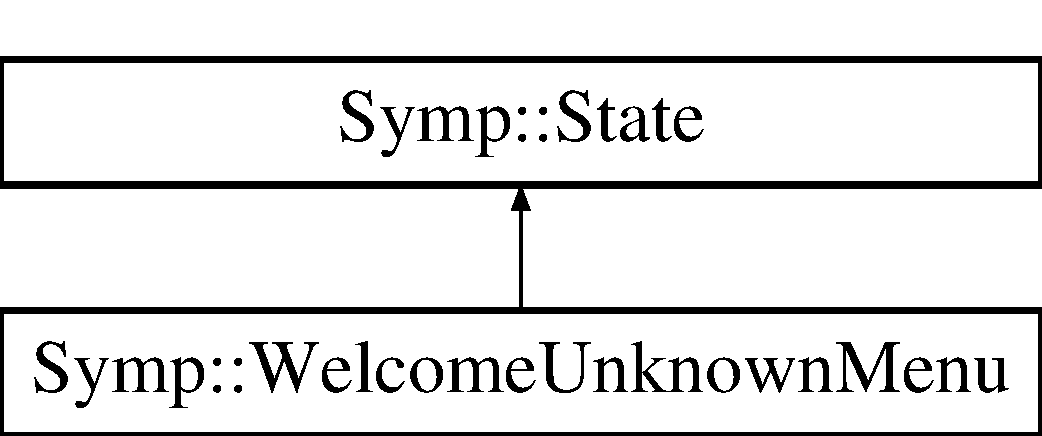
\includegraphics[height=2.000000cm]{class_symp_1_1_welcome_unknown_menu}
\end{center}
\end{figure}
\subsection*{Public Member Functions}
\begin{DoxyCompactItemize}
\item 
\hyperlink{class_symp_1_1_welcome_unknown_menu_a7510d4b914b2ffa4140a4f26c423e382}{Welcome\-Unknown\-Menu} ()
\begin{DoxyCompactList}\small\item\em \hyperlink{class_symp_1_1_welcome_unknown_menu}{Welcome\-Unknown\-Menu} constructor Responsible for the initialization of the private attributes of the \hyperlink{class_symp_1_1_welcome_unknown_menu_a7510d4b914b2ffa4140a4f26c423e382}{Welcome\-Unknown\-Menu} class. This function is not responsible for drawing the graphical elements that compose the menu, the \hyperlink{class_symp_1_1_welcome_unknown_menu_a57182187076a7158a71ad395bfdc1202}{init()} function is. \end{DoxyCompactList}\item 
\hyperlink{class_symp_1_1_welcome_unknown_menu_a2df66f757fe7a5bbad3c3bdd3d5f43ad}{$\sim$\-Welcome\-Unknown\-Menu} ()
\item 
virtual void \hyperlink{class_symp_1_1_welcome_unknown_menu_a57182187076a7158a71ad395bfdc1202}{init} ()
\begin{DoxyCompactList}\small\item\em \hyperlink{class_symp_1_1_welcome_unknown_menu}{Welcome\-Unknown\-Menu} elements initialization The elements that compose the menu are created in this function. \end{DoxyCompactList}\item 
virtual void \hyperlink{class_symp_1_1_welcome_unknown_menu_aab730d45332061d9028802a34bf307a4}{handle\-Mouse\-Clic} (int mouse\-X, int mouse\-Y)
\begin{DoxyCompactList}\small\item\em Handle mouse clic events. \end{DoxyCompactList}\item 
virtual void \hyperlink{class_symp_1_1_welcome_unknown_menu_a6d4dcd79840d2ae8b0ad17759c3ffdac}{key\-Down\-Pressed} ()
\begin{DoxyCompactList}\small\item\em Handle key down event. \end{DoxyCompactList}\item 
virtual void \hyperlink{class_symp_1_1_welcome_unknown_menu_a2fcfb802e8398d1a5178b904841650fb}{key\-Up\-Pressed} ()
\begin{DoxyCompactList}\small\item\em Handle key up event. \end{DoxyCompactList}\end{DoxyCompactItemize}


\subsection{Detailed Description}
the \hyperlink{class_symp_1_1_state_ad44d90b6e1b68eb021ceaa0cb98141a4}{State} interface for implementing the \hyperlink{class_symp_1_1_state}{State} Machine Pattern This Menu is the first menu of the application in case no players data have been found in the resources. The user can only create a new game or quit the application. \begin{DoxySeeAlso}{See Also}
\hyperlink{class_symp_1_1_new_game_menu}{New\-Game\-Menu} 

\hyperlink{class_symp_1_1_state}{State} 

\hyperlink{class_symp_1_1_game_manager}{Game\-Manager} 

\hyperlink{class_symp_1_1_manage_games_menu}{Manage\-Games\-Menu} 

\hyperlink{class_symp_1_1_menu_manager}{Menu\-Manager} 
\end{DoxySeeAlso}


Definition at line 20 of file Welcome\-Unknown\-Menu.\-h.



\subsection{Constructor \& Destructor Documentation}
\hypertarget{class_symp_1_1_welcome_unknown_menu_a7510d4b914b2ffa4140a4f26c423e382}{\index{Symp\-::\-Welcome\-Unknown\-Menu@{Symp\-::\-Welcome\-Unknown\-Menu}!Welcome\-Unknown\-Menu@{Welcome\-Unknown\-Menu}}
\index{Welcome\-Unknown\-Menu@{Welcome\-Unknown\-Menu}!Symp::WelcomeUnknownMenu@{Symp\-::\-Welcome\-Unknown\-Menu}}
\subsubsection[{Welcome\-Unknown\-Menu}]{\setlength{\rightskip}{0pt plus 5cm}Symp\-::\-Welcome\-Unknown\-Menu\-::\-Welcome\-Unknown\-Menu (
\begin{DoxyParamCaption}
{}
\end{DoxyParamCaption}
)}}\label{class_symp_1_1_welcome_unknown_menu_a7510d4b914b2ffa4140a4f26c423e382}


\hyperlink{class_symp_1_1_welcome_unknown_menu}{Welcome\-Unknown\-Menu} constructor Responsible for the initialization of the private attributes of the \hyperlink{class_symp_1_1_welcome_unknown_menu_a7510d4b914b2ffa4140a4f26c423e382}{Welcome\-Unknown\-Menu} class. This function is not responsible for drawing the graphical elements that compose the menu, the \hyperlink{class_symp_1_1_welcome_unknown_menu_a57182187076a7158a71ad395bfdc1202}{init()} function is. 


\begin{DoxyParams}{Parameters}
{\em p\-Menu\-Manager} & the reference to the \#\-Menu\-Manager \\
\hline
\end{DoxyParams}
\begin{DoxySeeAlso}{See Also}
\hyperlink{class_symp_1_1_player}{Player} 

\hyperlink{class_symp_1_1_menu_manager}{Menu\-Manager} 

\hyperlink{class_symp_1_1_state}{State} 

\hyperlink{class_symp_1_1_welcome_unknown_menu_a57182187076a7158a71ad395bfdc1202}{init()} 

\hyperlink{class_symp_1_1_welcome_unknown_menu_a2df66f757fe7a5bbad3c3bdd3d5f43ad}{$\sim$\-Welcome\-Unknown\-Menu()}) 
\end{DoxySeeAlso}


Definition at line 23 of file Welcome\-Unknown\-Menu.\-cpp.

\hypertarget{class_symp_1_1_welcome_unknown_menu_a2df66f757fe7a5bbad3c3bdd3d5f43ad}{\index{Symp\-::\-Welcome\-Unknown\-Menu@{Symp\-::\-Welcome\-Unknown\-Menu}!$\sim$\-Welcome\-Unknown\-Menu@{$\sim$\-Welcome\-Unknown\-Menu}}
\index{$\sim$\-Welcome\-Unknown\-Menu@{$\sim$\-Welcome\-Unknown\-Menu}!Symp::WelcomeUnknownMenu@{Symp\-::\-Welcome\-Unknown\-Menu}}
\subsubsection[{$\sim$\-Welcome\-Unknown\-Menu}]{\setlength{\rightskip}{0pt plus 5cm}Symp\-::\-Welcome\-Unknown\-Menu\-::$\sim$\-Welcome\-Unknown\-Menu (
\begin{DoxyParamCaption}
{}
\end{DoxyParamCaption}
)\hspace{0.3cm}{\ttfamily [inline]}}}\label{class_symp_1_1_welcome_unknown_menu_a2df66f757fe7a5bbad3c3bdd3d5f43ad}


Definition at line 23 of file Welcome\-Unknown\-Menu.\-h.



\subsection{Member Function Documentation}
\hypertarget{class_symp_1_1_welcome_unknown_menu_aab730d45332061d9028802a34bf307a4}{\index{Symp\-::\-Welcome\-Unknown\-Menu@{Symp\-::\-Welcome\-Unknown\-Menu}!handle\-Mouse\-Clic@{handle\-Mouse\-Clic}}
\index{handle\-Mouse\-Clic@{handle\-Mouse\-Clic}!Symp::WelcomeUnknownMenu@{Symp\-::\-Welcome\-Unknown\-Menu}}
\subsubsection[{handle\-Mouse\-Clic}]{\setlength{\rightskip}{0pt plus 5cm}void Symp\-::\-Welcome\-Unknown\-Menu\-::handle\-Mouse\-Clic (
\begin{DoxyParamCaption}
\item[{int}]{mouse\-X, }
\item[{int}]{mouse\-Y}
\end{DoxyParamCaption}
)\hspace{0.3cm}{\ttfamily [virtual]}}}\label{class_symp_1_1_welcome_unknown_menu_aab730d45332061d9028802a34bf307a4}


Handle mouse clic events. 


\begin{DoxyParams}{Parameters}
{\em mouse\-X} & the x coordinate of the mouse position \\
\hline
{\em mouse\-Y} & the y coordinate of the mouse position \\
\hline
\end{DoxyParams}
\begin{DoxySeeAlso}{See Also}
\hyperlink{class_symp_1_1_menu_manager}{Menu\-Manager} 

\hyperlink{class_symp_1_1_state}{State} 

\hyperlink{class_symp_1_1_input_manager}{Input\-Manager} 

\hyperlink{class_symp_1_1_welcome_unknown_menu_a57182187076a7158a71ad395bfdc1202}{init()} 
\end{DoxySeeAlso}


Implements \hyperlink{class_symp_1_1_state_a23e468a10d9be4c79d17e22d1d5ef478}{Symp\-::\-State}.



Definition at line 83 of file Welcome\-Unknown\-Menu.\-cpp.

\hypertarget{class_symp_1_1_welcome_unknown_menu_a57182187076a7158a71ad395bfdc1202}{\index{Symp\-::\-Welcome\-Unknown\-Menu@{Symp\-::\-Welcome\-Unknown\-Menu}!init@{init}}
\index{init@{init}!Symp::WelcomeUnknownMenu@{Symp\-::\-Welcome\-Unknown\-Menu}}
\subsubsection[{init}]{\setlength{\rightskip}{0pt plus 5cm}void Symp\-::\-Welcome\-Unknown\-Menu\-::init (
\begin{DoxyParamCaption}
{}
\end{DoxyParamCaption}
)\hspace{0.3cm}{\ttfamily [virtual]}}}\label{class_symp_1_1_welcome_unknown_menu_a57182187076a7158a71ad395bfdc1202}


\hyperlink{class_symp_1_1_welcome_unknown_menu}{Welcome\-Unknown\-Menu} elements initialization The elements that compose the menu are created in this function. 

\begin{DoxySeeAlso}{See Also}
\hyperlink{class_symp_1_1_player}{Player} 

\hyperlink{class_symp_1_1_menu_manager}{Menu\-Manager} 

\hyperlink{class_symp_1_1_state}{State} 

end() 

\hyperlink{class_symp_1_1_welcome_unknown_menu_a7510d4b914b2ffa4140a4f26c423e382}{Welcome\-Unknown\-Menu()} 
\end{DoxySeeAlso}


Implements \hyperlink{class_symp_1_1_state_a2c1c597b1235128a356c7529c42fdec3}{Symp\-::\-State}.



Definition at line 37 of file Welcome\-Unknown\-Menu.\-cpp.

\hypertarget{class_symp_1_1_welcome_unknown_menu_a6d4dcd79840d2ae8b0ad17759c3ffdac}{\index{Symp\-::\-Welcome\-Unknown\-Menu@{Symp\-::\-Welcome\-Unknown\-Menu}!key\-Down\-Pressed@{key\-Down\-Pressed}}
\index{key\-Down\-Pressed@{key\-Down\-Pressed}!Symp::WelcomeUnknownMenu@{Symp\-::\-Welcome\-Unknown\-Menu}}
\subsubsection[{key\-Down\-Pressed}]{\setlength{\rightskip}{0pt plus 5cm}void Symp\-::\-Welcome\-Unknown\-Menu\-::key\-Down\-Pressed (
\begin{DoxyParamCaption}
{}
\end{DoxyParamCaption}
)\hspace{0.3cm}{\ttfamily [virtual]}}}\label{class_symp_1_1_welcome_unknown_menu_a6d4dcd79840d2ae8b0ad17759c3ffdac}


Handle key down event. 

\begin{DoxySeeAlso}{See Also}
\hyperlink{class_symp_1_1_menu_manager}{Menu\-Manager} 

\hyperlink{class_symp_1_1_state}{State} 

\hyperlink{class_symp_1_1_input_manager}{Input\-Manager} 

\hyperlink{class_symp_1_1_welcome_unknown_menu_a57182187076a7158a71ad395bfdc1202}{init()} 
\end{DoxySeeAlso}


Implements \hyperlink{class_symp_1_1_state_ac9ff920d185cdc17c9bc3ac63b40c62d}{Symp\-::\-State}.



Definition at line 102 of file Welcome\-Unknown\-Menu.\-cpp.

\hypertarget{class_symp_1_1_welcome_unknown_menu_a2fcfb802e8398d1a5178b904841650fb}{\index{Symp\-::\-Welcome\-Unknown\-Menu@{Symp\-::\-Welcome\-Unknown\-Menu}!key\-Up\-Pressed@{key\-Up\-Pressed}}
\index{key\-Up\-Pressed@{key\-Up\-Pressed}!Symp::WelcomeUnknownMenu@{Symp\-::\-Welcome\-Unknown\-Menu}}
\subsubsection[{key\-Up\-Pressed}]{\setlength{\rightskip}{0pt plus 5cm}void Symp\-::\-Welcome\-Unknown\-Menu\-::key\-Up\-Pressed (
\begin{DoxyParamCaption}
{}
\end{DoxyParamCaption}
)\hspace{0.3cm}{\ttfamily [virtual]}}}\label{class_symp_1_1_welcome_unknown_menu_a2fcfb802e8398d1a5178b904841650fb}


Handle key up event. 

\begin{DoxySeeAlso}{See Also}
\hyperlink{class_symp_1_1_menu_manager}{Menu\-Manager} 

\hyperlink{class_symp_1_1_state}{State} 

\hyperlink{class_symp_1_1_input_manager}{Input\-Manager} 

\hyperlink{class_symp_1_1_welcome_unknown_menu_a57182187076a7158a71ad395bfdc1202}{init()} 
\end{DoxySeeAlso}


Implements \hyperlink{class_symp_1_1_state_a67d0fc2a02808bbcfdb06935c3be404f}{Symp\-::\-State}.



Definition at line 112 of file Welcome\-Unknown\-Menu.\-cpp.



The documentation for this class was generated from the following files\-:\begin{DoxyCompactItemize}
\item 
/home/cecilia/\-Documents/\-Symptogen/src/menu/\hyperlink{_welcome_unknown_menu_8h}{Welcome\-Unknown\-Menu.\-h}\item 
/home/cecilia/\-Documents/\-Symptogen/src/menu/\hyperlink{_welcome_unknown_menu_8cpp}{Welcome\-Unknown\-Menu.\-cpp}\end{DoxyCompactItemize}

\hypertarget{class_symp_1_1_window}{\section{Symp\-:\-:Window Class Reference}
\label{class_symp_1_1_window}\index{Symp\-::\-Window@{Symp\-::\-Window}}
}


{\ttfamily \#include $<$Window.\-h$>$}

\subsection*{Public Member Functions}
\begin{DoxyCompactItemize}
\item 
\hyperlink{class_symp_1_1_window_aa8cecc7f17dca9576ddf1e74d1891202}{Window} ()
\item 
void \hyperlink{class_symp_1_1_window_acffad4691bf25bdf3aff62d38fc7d927}{set\-Window} (I\-N\-D\-\_\-\-Window $\ast$p\-Window)
\item 
void \hyperlink{class_symp_1_1_window_a24c8fe288a988d6bd909c60615d0ca1d}{set\-Cursor} (bool p\-Enable)
\item 
I\-N\-D\-\_\-\-Window $\ast$ \hyperlink{class_symp_1_1_window_a1754691a1c7d5f0f8b7ea2a24763a1b0}{get\-I\-N\-D\-\_\-\-Window} ()
\end{DoxyCompactItemize}


\subsection{Detailed Description}
Facade of I\-N\-D\-\_\-\-Window. 

Definition at line 12 of file Window.\-h.



\subsection{Constructor \& Destructor Documentation}
\hypertarget{class_symp_1_1_window_aa8cecc7f17dca9576ddf1e74d1891202}{\index{Symp\-::\-Window@{Symp\-::\-Window}!Window@{Window}}
\index{Window@{Window}!Symp::Window@{Symp\-::\-Window}}
\subsubsection[{Window}]{\setlength{\rightskip}{0pt plus 5cm}Symp\-::\-Window\-::\-Window (
\begin{DoxyParamCaption}
{}
\end{DoxyParamCaption}
)}}\label{class_symp_1_1_window_aa8cecc7f17dca9576ddf1e74d1891202}


Definition at line 5 of file Window.\-cpp.



\subsection{Member Function Documentation}
\hypertarget{class_symp_1_1_window_a1754691a1c7d5f0f8b7ea2a24763a1b0}{\index{Symp\-::\-Window@{Symp\-::\-Window}!get\-I\-N\-D\-\_\-\-Window@{get\-I\-N\-D\-\_\-\-Window}}
\index{get\-I\-N\-D\-\_\-\-Window@{get\-I\-N\-D\-\_\-\-Window}!Symp::Window@{Symp\-::\-Window}}
\subsubsection[{get\-I\-N\-D\-\_\-\-Window}]{\setlength{\rightskip}{0pt plus 5cm}I\-N\-D\-\_\-\-Window$\ast$ Symp\-::\-Window\-::get\-I\-N\-D\-\_\-\-Window (
\begin{DoxyParamCaption}
{}
\end{DoxyParamCaption}
)\hspace{0.3cm}{\ttfamily [inline]}}}\label{class_symp_1_1_window_a1754691a1c7d5f0f8b7ea2a24763a1b0}


Definition at line 19 of file Window.\-h.

\hypertarget{class_symp_1_1_window_a24c8fe288a988d6bd909c60615d0ca1d}{\index{Symp\-::\-Window@{Symp\-::\-Window}!set\-Cursor@{set\-Cursor}}
\index{set\-Cursor@{set\-Cursor}!Symp::Window@{Symp\-::\-Window}}
\subsubsection[{set\-Cursor}]{\setlength{\rightskip}{0pt plus 5cm}void Symp\-::\-Window\-::set\-Cursor (
\begin{DoxyParamCaption}
\item[{bool}]{p\-Enable}
\end{DoxyParamCaption}
)}}\label{class_symp_1_1_window_a24c8fe288a988d6bd909c60615d0ca1d}


Definition at line 13 of file Window.\-cpp.

\hypertarget{class_symp_1_1_window_acffad4691bf25bdf3aff62d38fc7d927}{\index{Symp\-::\-Window@{Symp\-::\-Window}!set\-Window@{set\-Window}}
\index{set\-Window@{set\-Window}!Symp::Window@{Symp\-::\-Window}}
\subsubsection[{set\-Window}]{\setlength{\rightskip}{0pt plus 5cm}void Symp\-::\-Window\-::set\-Window (
\begin{DoxyParamCaption}
\item[{I\-N\-D\-\_\-\-Window $\ast$}]{p\-Window}
\end{DoxyParamCaption}
)}}\label{class_symp_1_1_window_acffad4691bf25bdf3aff62d38fc7d927}


Definition at line 9 of file Window.\-cpp.



The documentation for this class was generated from the following files\-:\begin{DoxyCompactItemize}
\item 
/home/cecilia/\-Documents/\-Symptogen/src/render/\hyperlink{_window_8h}{Window.\-h}\item 
/home/cecilia/\-Documents/\-Symptogen/src/render/\hyperlink{_window_8cpp}{Window.\-cpp}\end{DoxyCompactItemize}

\chapter{File Documentation}
\hypertarget{_entity_manager_8cpp}{\section{/home/cecilia/\-Documents/\-Symptogen/src/\-Entity\-Manager.cpp File Reference}
\label{_entity_manager_8cpp}\index{/home/cecilia/\-Documents/\-Symptogen/src/\-Entity\-Manager.\-cpp@{/home/cecilia/\-Documents/\-Symptogen/src/\-Entity\-Manager.\-cpp}}
}
{\ttfamily \#include \char`\"{}Entity\-Manager.\-h\char`\"{}}\\*
{\ttfamily \#include \char`\"{}sound/\-Sound\-Manager.\-h\char`\"{}}\\*
{\ttfamily \#include \char`\"{}power/\-Fever.\-h\char`\"{}}\\*
{\ttfamily \#include \char`\"{}power/\-Sneeze.\-h\char`\"{}}\\*
{\ttfamily \#include $<$stdexcept$>$}\\*
{\ttfamily \#include $<$ctime$>$}\\*
\subsection*{Namespaces}
\begin{DoxyCompactItemize}
\item 
\hyperlink{namespace_symp}{Symp}
\end{DoxyCompactItemize}
\subsection*{Constant Groups}
\begin{DoxyCompactItemize}
\item 
\hyperlink{namespace_symp}{Symp}
\end{DoxyCompactItemize}

\hypertarget{_entity_manager_8h}{\section{/home/cecilia/\-Documents/\-Symptogen/src/\-Entity\-Manager.h File Reference}
\label{_entity_manager_8h}\index{/home/cecilia/\-Documents/\-Symptogen/src/\-Entity\-Manager.\-h@{/home/cecilia/\-Documents/\-Symptogen/src/\-Entity\-Manager.\-h}}
}
{\ttfamily \#include $<$vector$>$}\\*
{\ttfamily \#include $<$array$>$}\\*
{\ttfamily \#include $<$Indie.\-h$>$}\\*
{\ttfamily \#include $<$I\-N\-D\-\_\-\-Entity2d.\-h$>$}\\*
{\ttfamily \#include $<$I\-N\-D\-\_\-\-Entity2d\-Manager.\-h$>$}\\*
{\ttfamily \#include \char`\"{}util/\-Singleton.\-h\char`\"{}}\\*
{\ttfamily \#include \char`\"{}render/\-Render.\-h\char`\"{}}\\*
{\ttfamily \#include \char`\"{}render/\-Render\-Entity.\-h\char`\"{}}\\*
{\ttfamily \#include \char`\"{}physic/\-Physical\-Entity.\-h\char`\"{}}\\*
{\ttfamily \#include \char`\"{}physic/\-Physical\-World.\-h\char`\"{}}\\*
{\ttfamily \#include \char`\"{}sound/\-Sound\-Entity.\-h\char`\"{}}\\*
{\ttfamily \#include \char`\"{}power/\-Power.\-h\char`\"{}}\\*
\subsection*{Classes}
\begin{DoxyCompactItemize}
\item 
class \hyperlink{class_symp_1_1_entity_manager}{Symp\-::\-Entity\-Manager}
\end{DoxyCompactItemize}
\subsection*{Namespaces}
\begin{DoxyCompactItemize}
\item 
\hyperlink{namespace_symp}{Symp}
\end{DoxyCompactItemize}
\subsection*{Constant Groups}
\begin{DoxyCompactItemize}
\item 
\hyperlink{namespace_symp}{Symp}
\end{DoxyCompactItemize}
\subsection*{Enumerations}
\begin{DoxyCompactItemize}
\item 
enum \hyperlink{namespace_symp_a303925db810fa122d017c4001bfa5e88}{Symp\-::\-Dino\-Action} \{ \\*
\hyperlink{namespace_symp_a303925db810fa122d017c4001bfa5e88a6790a525c17b14fe30e9cd196a5e43d1}{Symp\-::\-Stop\-Normal}, 
\hyperlink{namespace_symp_a303925db810fa122d017c4001bfa5e88aa186700234e7017346b4f1faad3d897b}{Symp\-::\-Stop\-Fever}, 
\hyperlink{namespace_symp_a303925db810fa122d017c4001bfa5e88a7445f9100f6d962e7d9a8fa155cdf2a2}{Symp\-::\-Stop\-Hypothermia}, 
\hyperlink{namespace_symp_a303925db810fa122d017c4001bfa5e88adc098df8f0c3c54a54f3821f0c804351}{Symp\-::\-Stop\-Shivering}, 
\\*
\hyperlink{namespace_symp_a303925db810fa122d017c4001bfa5e88a8167a726294616defad0afb74bfbf290}{Symp\-::\-Walk\-Normal}, 
\hyperlink{namespace_symp_a303925db810fa122d017c4001bfa5e88a333bc3b10a117b9fd459e2f3fae422ce}{Symp\-::\-Walk\-Fever}, 
\hyperlink{namespace_symp_a303925db810fa122d017c4001bfa5e88a5a32a2e75b36addf2f26f022ee4f4ac2}{Symp\-::\-Walk\-Hypothermia}, 
\hyperlink{namespace_symp_a303925db810fa122d017c4001bfa5e88ac6dda8c07b5b6b1ceab3070aa6afa180}{Symp\-::\-Walk\-Shivering}, 
\\*
\hyperlink{namespace_symp_a303925db810fa122d017c4001bfa5e88af2e207c92737431950a7bd3641bab549}{Symp\-::\-Jump}, 
\hyperlink{namespace_symp_a303925db810fa122d017c4001bfa5e88a63a3a9a767b7dc709ddbf829d9640a02}{Symp\-::\-Death\-Normal}, 
\hyperlink{namespace_symp_a303925db810fa122d017c4001bfa5e88a40adc2c2ccec6268983e08fbb7e5441e}{Symp\-::\-Death\-Fever}, 
\hyperlink{namespace_symp_a303925db810fa122d017c4001bfa5e88afa6f0fda267437e5a3112a47560c9569}{Symp\-::\-Death\-Hypothermia}, 
\\*
\hyperlink{namespace_symp_a303925db810fa122d017c4001bfa5e88a3ec52f1e8e27cf00c64afdf99e7012bb}{Symp\-::\-Sneezing}, 
\hyperlink{namespace_symp_a303925db810fa122d017c4001bfa5e88a7be96c60638459db1eb6038ff97f9385}{Symp\-::\-Fever\-Sneezing}, 
\hyperlink{namespace_symp_a303925db810fa122d017c4001bfa5e88a4aea186f9692d2bca1cf75e46b20c68d}{Symp\-::\-Cold\-Sneezing}, 
\hyperlink{namespace_symp_a303925db810fa122d017c4001bfa5e88a4bfeb5dbe245f022ad26812a2ea7168f}{Symp\-::\-Headache\-Action}
 \}
\item 
enum \hyperlink{namespace_symp_a2b868de1f6f86f455f39dfa63028859c}{Symp\-::\-Flower\-Action} \{ \hyperlink{namespace_symp_a2b868de1f6f86f455f39dfa63028859ca4588318618fd0ad6a4499f3430e038d4}{Symp\-::\-Normal}, 
\hyperlink{namespace_symp_a2b868de1f6f86f455f39dfa63028859caf105414e645c4198cd56c1cd3936a458}{Symp\-::\-Collide\-Dino}
 \}
\item 
enum \hyperlink{namespace_symp_a9f891c0e98f2864e7b687d741bf032d7}{Symp\-::\-Destructible\-Object\-Action} \{ \hyperlink{namespace_symp_a9f891c0e98f2864e7b687d741bf032d7a6bd253cbfd8722c2aa04b32e1ab9e3ed}{Symp\-::\-Normal\-Box}, 
\hyperlink{namespace_symp_a9f891c0e98f2864e7b687d741bf032d7a3816c03b90d4074e920820074c538bc0}{Symp\-::\-By\-Flames}, 
\hyperlink{namespace_symp_a9f891c0e98f2864e7b687d741bf032d7a22282e8324d516b014aab643362a4224}{Symp\-::\-By\-Shivering}
 \}
\end{DoxyCompactItemize}

\hypertarget{_game_manager_8cpp}{\section{/home/cecilia/\-Documents/\-Symptogen/src/\-Game\-Manager.cpp File Reference}
\label{_game_manager_8cpp}\index{/home/cecilia/\-Documents/\-Symptogen/src/\-Game\-Manager.\-cpp@{/home/cecilia/\-Documents/\-Symptogen/src/\-Game\-Manager.\-cpp}}
}
{\ttfamily \#include $<$Indie.\-h$>$}\\*
{\ttfamily \#include \char`\"{}Game\-Manager.\-h\char`\"{}}\\*
{\ttfamily \#include \char`\"{}menu/\-Pause\-Menu.\-h\char`\"{}}\\*
{\ttfamily \#include \char`\"{}menu/\-Player.\-h\char`\"{}}\\*
{\ttfamily \#include \char`\"{}power/\-Power.\-h\char`\"{}}\\*
{\ttfamily \#include \char`\"{}power/\-Sneeze.\-h\char`\"{}}\\*
{\ttfamily \#include \char`\"{}power/\-Fever.\-h\char`\"{}}\\*
{\ttfamily \#include \char`\"{}power/\-Headache.\-h\char`\"{}}\\*
{\ttfamily \#include $<$X11/\-Xlib.\-h$>$}\\*
\subsection*{Namespaces}
\begin{DoxyCompactItemize}
\item 
\hyperlink{namespace_symp}{Symp}
\end{DoxyCompactItemize}
\subsection*{Constant Groups}
\begin{DoxyCompactItemize}
\item 
\hyperlink{namespace_symp}{Symp}
\end{DoxyCompactItemize}
\subsection*{Variables}
\begin{DoxyCompactItemize}
\item 
int \hyperlink{namespace_symp_a13b9ebf55d22fb1ad248558acfd4cec6}{Symp\-::g\-\_\-\-Window\-Width} = 1365
\item 
int \hyperlink{namespace_symp_a09ae4e5593b8a85ecf79b0db00377f1f}{Symp\-::g\-\_\-\-Window\-Height} = 767
\end{DoxyCompactItemize}

\hypertarget{_game_manager_8h}{\section{/home/cecilia/\-Documents/\-Symptogen/src/\-Game\-Manager.h File Reference}
\label{_game_manager_8h}\index{/home/cecilia/\-Documents/\-Symptogen/src/\-Game\-Manager.\-h@{/home/cecilia/\-Documents/\-Symptogen/src/\-Game\-Manager.\-h}}
}
{\ttfamily \#include \char`\"{}render/\-Window.\-h\char`\"{}}\\*
{\ttfamily \#include \char`\"{}render/\-Render.\-h\char`\"{}}\\*
{\ttfamily \#include \char`\"{}input/\-Input\-Manager.\-h\char`\"{}}\\*
{\ttfamily \#include \char`\"{}sound/\-Sound\-Manager.\-h\char`\"{}}\\*
{\ttfamily \#include \char`\"{}persistence/\-Parser.\-h\char`\"{}}\\*
{\ttfamily \#include \char`\"{}menu/\-Menu\-Manager.\-h\char`\"{}}\\*
{\ttfamily \#include \char`\"{}Entity\-Manager.\-h\char`\"{}}\\*
{\ttfamily \#include \char`\"{}util/\-Singleton.\-h\char`\"{}}\\*
\subsection*{Classes}
\begin{DoxyCompactItemize}
\item 
class \hyperlink{class_symp_1_1_game_manager}{Symp\-::\-Game\-Manager}
\end{DoxyCompactItemize}
\subsection*{Namespaces}
\begin{DoxyCompactItemize}
\item 
\hyperlink{namespace_symp}{Symp}
\end{DoxyCompactItemize}
\subsection*{Constant Groups}
\begin{DoxyCompactItemize}
\item 
\hyperlink{namespace_symp}{Symp}
\end{DoxyCompactItemize}

\hypertarget{_input_manager_8cpp}{\section{/home/cecilia/\-Documents/\-Symptogen/src/input/\-Input\-Manager.cpp File Reference}
\label{_input_manager_8cpp}\index{/home/cecilia/\-Documents/\-Symptogen/src/input/\-Input\-Manager.\-cpp@{/home/cecilia/\-Documents/\-Symptogen/src/input/\-Input\-Manager.\-cpp}}
}
{\ttfamily \#include \char`\"{}Input\-Manager.\-h\char`\"{}}\\*
\subsection*{Namespaces}
\begin{DoxyCompactItemize}
\item 
\hyperlink{namespace_symp}{Symp}
\end{DoxyCompactItemize}
\subsection*{Constant Groups}
\begin{DoxyCompactItemize}
\item 
\hyperlink{namespace_symp}{Symp}
\end{DoxyCompactItemize}

\hypertarget{_input_manager_8h}{\section{/home/cecilia/\-Documents/\-Symptogen/src/input/\-Input\-Manager.h File Reference}
\label{_input_manager_8h}\index{/home/cecilia/\-Documents/\-Symptogen/src/input/\-Input\-Manager.\-h@{/home/cecilia/\-Documents/\-Symptogen/src/input/\-Input\-Manager.\-h}}
}
{\ttfamily \#include $<$Indie.\-h$>$}\\*
{\ttfamily \#include $<$I\-N\-D\-\_\-\-Input.\-h$>$}\\*
{\ttfamily \#include \char`\"{}../util/\-Singleton.\-h\char`\"{}}\\*
{\ttfamily \#include \char`\"{}../render/\-Render.\-h\char`\"{}}\\*
\subsection*{Classes}
\begin{DoxyCompactItemize}
\item 
class \hyperlink{class_symp_1_1_input_manager}{Symp\-::\-Input\-Manager}
\end{DoxyCompactItemize}
\subsection*{Namespaces}
\begin{DoxyCompactItemize}
\item 
\hyperlink{namespace_symp}{Symp}
\end{DoxyCompactItemize}
\subsection*{Constant Groups}
\begin{DoxyCompactItemize}
\item 
\hyperlink{namespace_symp}{Symp}
\end{DoxyCompactItemize}

\hypertarget{main_8cpp}{\section{/home/cecilia/\-Documents/\-Symptogen/src/main.cpp File Reference}
\label{main_8cpp}\index{/home/cecilia/\-Documents/\-Symptogen/src/main.\-cpp@{/home/cecilia/\-Documents/\-Symptogen/src/main.\-cpp}}
}
{\ttfamily \#include $<$iostream$>$}\\*
{\ttfamily \#include $<$fmod.\-h$>$}\\*
{\ttfamily \#include $<$fmod\-\_\-errors.\-h$>$}\\*
{\ttfamily \#include $<$Box2\-D/\-Box2\-D.\-h$>$}\\*
{\ttfamily \#include \char`\"{}Game\-Manager.\-h\char`\"{}}\\*
{\ttfamily \#include \char`\"{}sound/\-Sound\-Manager.\-h\char`\"{}}\\*
\subsection*{Variables}
\begin{DoxyCompactItemize}
\item 
\hyperlink{main_8cpp_a9717e7bbecb906637e86cef6da3d83c2}{return}
\end{DoxyCompactItemize}


\subsection{Variable Documentation}
\hypertarget{main_8cpp_a9717e7bbecb906637e86cef6da3d83c2}{\index{main.\-cpp@{main.\-cpp}!return@{return}}
\index{return@{return}!main.cpp@{main.\-cpp}}
\subsubsection[{return}]{\setlength{\rightskip}{0pt plus 5cm}return}}\label{main_8cpp_a9717e7bbecb906637e86cef6da3d83c2}


Definition at line 22 of file main.\-cpp.


\hypertarget{_button_8cpp}{\section{/home/cecilia/\-Documents/\-Symptogen/src/menu/\-Button.cpp File Reference}
\label{_button_8cpp}\index{/home/cecilia/\-Documents/\-Symptogen/src/menu/\-Button.\-cpp@{/home/cecilia/\-Documents/\-Symptogen/src/menu/\-Button.\-cpp}}
}
{\ttfamily \#include \char`\"{}Button.\-h\char`\"{}}\\*
\subsection*{Namespaces}
\begin{DoxyCompactItemize}
\item 
\hyperlink{namespace_symp}{Symp}
\end{DoxyCompactItemize}
\subsection*{Constant Groups}
\begin{DoxyCompactItemize}
\item 
\hyperlink{namespace_symp}{Symp}
\end{DoxyCompactItemize}

\hypertarget{_button_8h}{\section{/home/cecilia/\-Documents/\-Symptogen/src/menu/\-Button.h File Reference}
\label{_button_8h}\index{/home/cecilia/\-Documents/\-Symptogen/src/menu/\-Button.\-h@{/home/cecilia/\-Documents/\-Symptogen/src/menu/\-Button.\-h}}
}
{\ttfamily \#include \char`\"{}Gui\-Component.\-h\char`\"{}}\\*
{\ttfamily \#include \char`\"{}Text.\-h\char`\"{}}\\*
\subsection*{Classes}
\begin{DoxyCompactItemize}
\item 
class \hyperlink{class_symp_1_1_button}{Symp\-::\-Button}
\begin{DoxyCompactList}\small\item\em \hyperlink{class_symp_1_1_button}{Button} class. This class inherits the \hyperlink{class_symp_1_1_gui_component_a22124675c2976983ac18374f81cc3fb3}{Gui\-Component} class. A \hyperlink{class_symp_1_1_button_a2de1604451d582a7c2e22344305212e5}{Button} is a clickable and selectable component that can display text, or texture, or be customized with border or background. The simpliest way to use \hyperlink{class_symp_1_1_button_a2de1604451d582a7c2e22344305212e5}{Button} is with the \#\-Layout class, that handle the position and the size of the \hyperlink{class_symp_1_1_button_a2de1604451d582a7c2e22344305212e5}{Button}. The only paramters left are the color and the type of \hyperlink{class_symp_1_1_button_a2de1604451d582a7c2e22344305212e5}{Button} that will be rendered. \end{DoxyCompactList}\end{DoxyCompactItemize}
\subsection*{Namespaces}
\begin{DoxyCompactItemize}
\item 
\hyperlink{namespace_symp}{Symp}
\end{DoxyCompactItemize}
\subsection*{Constant Groups}
\begin{DoxyCompactItemize}
\item 
\hyperlink{namespace_symp}{Symp}
\end{DoxyCompactItemize}

\hypertarget{_choose_your_level_menu_8cpp}{\section{/home/cecilia/\-Documents/\-Symptogen/src/menu/\-Choose\-Your\-Level\-Menu.cpp File Reference}
\label{_choose_your_level_menu_8cpp}\index{/home/cecilia/\-Documents/\-Symptogen/src/menu/\-Choose\-Your\-Level\-Menu.\-cpp@{/home/cecilia/\-Documents/\-Symptogen/src/menu/\-Choose\-Your\-Level\-Menu.\-cpp}}
}
{\ttfamily \#include \char`\"{}Choose\-Your\-Level\-Menu.\-h\char`\"{}}\\*
{\ttfamily \#include $<$sstream$>$}\\*
\subsection*{Namespaces}
\begin{DoxyCompactItemize}
\item 
\hyperlink{namespace_symp}{Symp}
\end{DoxyCompactItemize}
\subsection*{Constant Groups}
\begin{DoxyCompactItemize}
\item 
\hyperlink{namespace_symp}{Symp}
\end{DoxyCompactItemize}

\hypertarget{_choose_your_level_menu_8h}{\section{/home/cecilia/\-Documents/\-Symptogen/src/menu/\-Choose\-Your\-Level\-Menu.h File Reference}
\label{_choose_your_level_menu_8h}\index{/home/cecilia/\-Documents/\-Symptogen/src/menu/\-Choose\-Your\-Level\-Menu.\-h@{/home/cecilia/\-Documents/\-Symptogen/src/menu/\-Choose\-Your\-Level\-Menu.\-h}}
}
{\ttfamily \#include \char`\"{}State.\-h\char`\"{}}\\*
{\ttfamily \#include \char`\"{}Menu\-Manager.\-h\char`\"{}}\\*
\subsection*{Classes}
\begin{DoxyCompactItemize}
\item 
class \hyperlink{class_symp_1_1_choose_your_level_menu}{Symp\-::\-Choose\-Your\-Level\-Menu}
\end{DoxyCompactItemize}
\subsection*{Namespaces}
\begin{DoxyCompactItemize}
\item 
\hyperlink{namespace_symp}{Symp}
\end{DoxyCompactItemize}
\subsection*{Constant Groups}
\begin{DoxyCompactItemize}
\item 
\hyperlink{namespace_symp}{Symp}
\end{DoxyCompactItemize}

\hypertarget{_gui_component_8cpp}{\section{/home/cecilia/\-Documents/\-Symptogen/src/menu/\-Gui\-Component.cpp File Reference}
\label{_gui_component_8cpp}\index{/home/cecilia/\-Documents/\-Symptogen/src/menu/\-Gui\-Component.\-cpp@{/home/cecilia/\-Documents/\-Symptogen/src/menu/\-Gui\-Component.\-cpp}}
}
{\ttfamily \#include \char`\"{}Gui\-Component.\-h\char`\"{}}\\*
{\ttfamily \#include $<$I\-N\-D\-\_\-\-Image.\-h$>$}\\*
{\ttfamily \#include $<$I\-N\-D\-\_\-\-Font.\-h$>$}\\*
{\ttfamily \#include $<$I\-N\-D\-\_\-\-Image\-Manager.\-h$>$}\\*
\subsection*{Namespaces}
\begin{DoxyCompactItemize}
\item 
\hyperlink{namespace_symp}{Symp}
\end{DoxyCompactItemize}
\subsection*{Constant Groups}
\begin{DoxyCompactItemize}
\item 
\hyperlink{namespace_symp}{Symp}
\end{DoxyCompactItemize}

\hypertarget{_gui_component_8h}{\section{/home/cecilia/\-Documents/\-Symptogen/src/menu/\-Gui\-Component.h File Reference}
\label{_gui_component_8h}\index{/home/cecilia/\-Documents/\-Symptogen/src/menu/\-Gui\-Component.\-h@{/home/cecilia/\-Documents/\-Symptogen/src/menu/\-Gui\-Component.\-h}}
}
{\ttfamily \#include $<$Indie.\-h$>$}\\*
{\ttfamily \#include $<$I\-N\-D\-\_\-\-Entity2d.\-h$>$}\\*
{\ttfamily \#include $<$I\-N\-D\-\_\-\-Entity2d\-Manager.\-h$>$}\\*
{\ttfamily \#include $<$I\-N\-D\-\_\-\-Surface.\-h$>$}\\*
{\ttfamily \#include $<$I\-N\-D\-\_\-\-Surface\-Manager.\-h$>$}\\*
{\ttfamily \#include $<$I\-N\-D\-\_\-\-Font.\-h$>$}\\*
{\ttfamily \#include \char`\"{}../render/\-Render.\-h\char`\"{}}\\*
\subsection*{Classes}
\begin{DoxyCompactItemize}
\item 
class \hyperlink{struct_symp_1_1_color}{Symp\-::\-Color}
\item 
class \hyperlink{class_symp_1_1_gui_component}{Symp\-::\-Gui\-Component}
\begin{DoxyCompactList}\small\item\em \hyperlink{class_symp_1_1_gui_component}{Gui\-Component} facade for the creation of Menu graphical entities The \hyperlink{class_symp_1_1_gui_component}{Gui\-Component} class implements a facade of the Indielib I\-N\-D\-\_\-\-E\-Ntity2d elements for the unique use of the menus. Each graphical element that compose a menu inherits from the \hyperlink{class_symp_1_1_gui_component}{Gui\-Component} class. The elements are stored in the \#\-Menu\-Manager class and rendered/updated by the \#\-Game\-Manager class. In order to use the Indielib architecture, this class implements static method for the I\-N\-D\-\_\-\-Image\-Manager, I\-N\-D\-\_\-\-Surface\-Manager and the I\-N\-D\-\_\-\-Font\-Manager initialization destruction. \end{DoxyCompactList}\end{DoxyCompactItemize}
\subsection*{Namespaces}
\begin{DoxyCompactItemize}
\item 
\hyperlink{namespace_symp}{Symp}
\end{DoxyCompactItemize}
\subsection*{Constant Groups}
\begin{DoxyCompactItemize}
\item 
\hyperlink{namespace_symp}{Symp}
\end{DoxyCompactItemize}

\hypertarget{_image_8cpp}{\section{/home/cecilia/\-Documents/\-Symptogen/src/menu/\-Image.cpp File Reference}
\label{_image_8cpp}\index{/home/cecilia/\-Documents/\-Symptogen/src/menu/\-Image.\-cpp@{/home/cecilia/\-Documents/\-Symptogen/src/menu/\-Image.\-cpp}}
}
{\ttfamily \#include \char`\"{}Image.\-h\char`\"{}}\\*
{\ttfamily \#include $<$algorithm$>$}\\*
\subsection*{Namespaces}
\begin{DoxyCompactItemize}
\item 
\hyperlink{namespace_symp}{Symp}
\end{DoxyCompactItemize}
\subsection*{Constant Groups}
\begin{DoxyCompactItemize}
\item 
\hyperlink{namespace_symp}{Symp}
\end{DoxyCompactItemize}

\hypertarget{_image_8h}{\section{/home/cecilia/\-Documents/\-Symptogen/src/menu/\-Image.h File Reference}
\label{_image_8h}\index{/home/cecilia/\-Documents/\-Symptogen/src/menu/\-Image.\-h@{/home/cecilia/\-Documents/\-Symptogen/src/menu/\-Image.\-h}}
}
{\ttfamily \#include \char`\"{}Gui\-Component.\-h\char`\"{}}\\*
\subsection*{Classes}
\begin{DoxyCompactItemize}
\item 
class \hyperlink{class_symp_1_1_image}{Symp\-::\-Image}
\end{DoxyCompactItemize}
\subsection*{Namespaces}
\begin{DoxyCompactItemize}
\item 
\hyperlink{namespace_symp}{Symp}
\end{DoxyCompactItemize}
\subsection*{Constant Groups}
\begin{DoxyCompactItemize}
\item 
\hyperlink{namespace_symp}{Symp}
\end{DoxyCompactItemize}
\subsection*{Enumerations}
\begin{DoxyCompactItemize}
\item 
enum \hyperlink{namespace_symp_a2d0f7a8e888710a800fc73cf4d1ed38d}{Symp\-::\-Aspect\-Ratio} \{ \hyperlink{namespace_symp_a2d0f7a8e888710a800fc73cf4d1ed38da37080ec8b73f25dde405c571395ac4a5}{Symp\-::\-I\-G\-N\-O\-R\-E\-\_\-\-A\-S\-P\-E\-C\-T\-\_\-\-R\-A\-T\-I\-O}, 
\hyperlink{namespace_symp_a2d0f7a8e888710a800fc73cf4d1ed38dac4b5023ead73709a534ee793228f8c1f}{Symp\-::\-K\-E\-E\-P\-\_\-\-A\-S\-P\-E\-C\-T\-\_\-\-R\-A\-T\-I\-O}, 
\hyperlink{namespace_symp_a2d0f7a8e888710a800fc73cf4d1ed38da27f6dac15bcc6e5e18a0044f7a73dd1e}{Symp\-::\-E\-X\-P\-A\-N\-D\-\_\-\-A\-S\-P\-E\-C\-T\-\_\-\-R\-A\-T\-I\-O}
 \}
\end{DoxyCompactItemize}

\hypertarget{_layout_8cpp}{\section{/home/cecilia/\-Documents/\-Symptogen/src/menu/\-Layout.cpp File Reference}
\label{_layout_8cpp}\index{/home/cecilia/\-Documents/\-Symptogen/src/menu/\-Layout.\-cpp@{/home/cecilia/\-Documents/\-Symptogen/src/menu/\-Layout.\-cpp}}
}
{\ttfamily \#include \char`\"{}Layout.\-h\char`\"{}}\\*
\subsection*{Namespaces}
\begin{DoxyCompactItemize}
\item 
\hyperlink{namespace_symp}{Symp}
\end{DoxyCompactItemize}
\subsection*{Constant Groups}
\begin{DoxyCompactItemize}
\item 
\hyperlink{namespace_symp}{Symp}
\end{DoxyCompactItemize}

\hypertarget{_layout_8h}{\section{/home/cecilia/\-Documents/\-Symptogen/src/menu/\-Layout.h File Reference}
\label{_layout_8h}\index{/home/cecilia/\-Documents/\-Symptogen/src/menu/\-Layout.\-h@{/home/cecilia/\-Documents/\-Symptogen/src/menu/\-Layout.\-h}}
}
{\ttfamily \#include \char`\"{}Gui\-Component.\-h\char`\"{}}\\*
{\ttfamily \#include $<$map$>$}\\*
\subsection*{Classes}
\begin{DoxyCompactItemize}
\item 
class \hyperlink{class_symp_1_1_layout}{Symp\-::\-Layout}
\end{DoxyCompactItemize}
\subsection*{Namespaces}
\begin{DoxyCompactItemize}
\item 
\hyperlink{namespace_symp}{Symp}
\end{DoxyCompactItemize}
\subsection*{Constant Groups}
\begin{DoxyCompactItemize}
\item 
\hyperlink{namespace_symp}{Symp}
\end{DoxyCompactItemize}
\subsection*{Enumerations}
\begin{DoxyCompactItemize}
\item 
enum \hyperlink{namespace_symp_a30499696a7501e2c08fdf0b3094484fb}{Symp\-::\-Layout\-Fill\-Attribute} \{ \hyperlink{namespace_symp_a30499696a7501e2c08fdf0b3094484fbae3bc233b48718363a050cd29711e3367}{Symp\-::\-B\-O\-R\-D\-E\-R}, 
\hyperlink{namespace_symp_a30499696a7501e2c08fdf0b3094484fbac3ac2f33d4d9f540529fc9ddcc9a689b}{Symp\-::\-B\-A\-C\-K\-G\-R\-O\-U\-N\-D}, 
\hyperlink{namespace_symp_a30499696a7501e2c08fdf0b3094484fbad44494c9dc289ce3c21d24da5a8e9ecc}{Symp\-::\-N\-O\-N\-E}
 \}
\end{DoxyCompactItemize}

\hypertarget{_line_edit_8cpp}{\section{/home/cecilia/\-Documents/\-Symptogen/src/menu/\-Line\-Edit.cpp File Reference}
\label{_line_edit_8cpp}\index{/home/cecilia/\-Documents/\-Symptogen/src/menu/\-Line\-Edit.\-cpp@{/home/cecilia/\-Documents/\-Symptogen/src/menu/\-Line\-Edit.\-cpp}}
}
{\ttfamily \#include \char`\"{}Line\-Edit.\-h\char`\"{}}\\*
{\ttfamily \#include \char`\"{}Menu\-Manager.\-h\char`\"{}}\\*
\subsection*{Namespaces}
\begin{DoxyCompactItemize}
\item 
\hyperlink{namespace_symp}{Symp}
\end{DoxyCompactItemize}
\subsection*{Constant Groups}
\begin{DoxyCompactItemize}
\item 
\hyperlink{namespace_symp}{Symp}
\end{DoxyCompactItemize}

\hypertarget{_line_edit_8h}{\section{/home/cecilia/\-Documents/\-Symptogen/src/menu/\-Line\-Edit.h File Reference}
\label{_line_edit_8h}\index{/home/cecilia/\-Documents/\-Symptogen/src/menu/\-Line\-Edit.\-h@{/home/cecilia/\-Documents/\-Symptogen/src/menu/\-Line\-Edit.\-h}}
}
{\ttfamily \#include \char`\"{}Gui\-Component.\-h\char`\"{}}\\*
{\ttfamily \#include \char`\"{}Image.\-h\char`\"{}}\\*
{\ttfamily \#include \char`\"{}Text.\-h\char`\"{}}\\*
\subsection*{Classes}
\begin{DoxyCompactItemize}
\item 
class \hyperlink{class_symp_1_1_line_edit}{Symp\-::\-Line\-Edit}
\end{DoxyCompactItemize}
\subsection*{Namespaces}
\begin{DoxyCompactItemize}
\item 
\hyperlink{namespace_symp}{Symp}
\end{DoxyCompactItemize}
\subsection*{Constant Groups}
\begin{DoxyCompactItemize}
\item 
\hyperlink{namespace_symp}{Symp}
\end{DoxyCompactItemize}

\hypertarget{_manage_games_menu_8cpp}{\section{/home/cecilia/\-Documents/\-Symptogen/src/menu/\-Manage\-Games\-Menu.cpp File Reference}
\label{_manage_games_menu_8cpp}\index{/home/cecilia/\-Documents/\-Symptogen/src/menu/\-Manage\-Games\-Menu.\-cpp@{/home/cecilia/\-Documents/\-Symptogen/src/menu/\-Manage\-Games\-Menu.\-cpp}}
}
{\ttfamily \#include \char`\"{}Manage\-Games\-Menu.\-h\char`\"{}}\\*
{\ttfamily \#include $<$sstream$>$}\\*
{\ttfamily \#include \char`\"{}New\-Game\-Menu.\-h\char`\"{}}\\*
{\ttfamily \#include \char`\"{}Choose\-Your\-Level\-Menu.\-h\char`\"{}}\\*
\subsection*{Namespaces}
\begin{DoxyCompactItemize}
\item 
\hyperlink{namespace_symp}{Symp}
\end{DoxyCompactItemize}
\subsection*{Constant Groups}
\begin{DoxyCompactItemize}
\item 
\hyperlink{namespace_symp}{Symp}
\end{DoxyCompactItemize}

\hypertarget{_manage_games_menu_8h}{\section{/home/cecilia/\-Documents/\-Symptogen/src/menu/\-Manage\-Games\-Menu.h File Reference}
\label{_manage_games_menu_8h}\index{/home/cecilia/\-Documents/\-Symptogen/src/menu/\-Manage\-Games\-Menu.\-h@{/home/cecilia/\-Documents/\-Symptogen/src/menu/\-Manage\-Games\-Menu.\-h}}
}
{\ttfamily \#include \char`\"{}State.\-h\char`\"{}}\\*
{\ttfamily \#include \char`\"{}Menu\-Manager.\-h\char`\"{}}\\*
\subsection*{Classes}
\begin{DoxyCompactItemize}
\item 
class \hyperlink{class_symp_1_1_manage_games_menu}{Symp\-::\-Manage\-Games\-Menu}
\end{DoxyCompactItemize}
\subsection*{Namespaces}
\begin{DoxyCompactItemize}
\item 
\hyperlink{namespace_symp}{Symp}
\end{DoxyCompactItemize}
\subsection*{Constant Groups}
\begin{DoxyCompactItemize}
\item 
\hyperlink{namespace_symp}{Symp}
\end{DoxyCompactItemize}

\hypertarget{_menu_manager_8cpp}{\section{/home/cecilia/\-Documents/\-Symptogen/src/menu/\-Menu\-Manager.cpp File Reference}
\label{_menu_manager_8cpp}\index{/home/cecilia/\-Documents/\-Symptogen/src/menu/\-Menu\-Manager.\-cpp@{/home/cecilia/\-Documents/\-Symptogen/src/menu/\-Menu\-Manager.\-cpp}}
}
{\ttfamily \#include \char`\"{}Menu\-Manager.\-h\char`\"{}}\\*
{\ttfamily \#include \char`\"{}Manage\-Games\-Menu.\-h\char`\"{}}\\*
{\ttfamily \#include \char`\"{}Welcome\-Unknown\-Menu.\-h\char`\"{}}\\*
{\ttfamily \#include \char`\"{}Welcome\-Last\-Player\-Menu.\-h\char`\"{}}\\*
{\ttfamily \#include \char`\"{}New\-Game\-Menu.\-h\char`\"{}}\\*
{\ttfamily \#include $<$Indie.\-h$>$}\\*
\subsection*{Namespaces}
\begin{DoxyCompactItemize}
\item 
\hyperlink{namespace_symp}{Symp}
\end{DoxyCompactItemize}
\subsection*{Constant Groups}
\begin{DoxyCompactItemize}
\item 
\hyperlink{namespace_symp}{Symp}
\end{DoxyCompactItemize}
\subsection*{Variables}
\begin{DoxyCompactItemize}
\item 
unsigned int \hyperlink{namespace_symp_a350b1cbffd0ded84bd0f5bb28bf9abe4}{Symp\-::g\-Total\-Level\-Number} = 10
\end{DoxyCompactItemize}

\hypertarget{_menu_manager_8h}{\section{/home/cecilia/\-Documents/\-Symptogen/src/menu/\-Menu\-Manager.h File Reference}
\label{_menu_manager_8h}\index{/home/cecilia/\-Documents/\-Symptogen/src/menu/\-Menu\-Manager.\-h@{/home/cecilia/\-Documents/\-Symptogen/src/menu/\-Menu\-Manager.\-h}}
}
{\ttfamily \#include $<$iostream$>$}\\*
{\ttfamily \#include $<$deque$>$}\\*
{\ttfamily \#include $<$Indie.\-h$>$}\\*
{\ttfamily \#include $<$I\-N\-D\-\_\-\-Entity2d\-Manager.\-h$>$}\\*
{\ttfamily \#include \char`\"{}../util/\-Singleton.\-h\char`\"{}}\\*
{\ttfamily \#include \char`\"{}Player.\-h\char`\"{}}\\*
{\ttfamily \#include \char`\"{}State.\-h\char`\"{}}\\*
{\ttfamily \#include \char`\"{}Layout.\-h\char`\"{}}\\*
{\ttfamily \#include \char`\"{}Button.\-h\char`\"{}}\\*
{\ttfamily \#include \char`\"{}Image.\-h\char`\"{}}\\*
{\ttfamily \#include \char`\"{}Line\-Edit.\-h\char`\"{}}\\*
{\ttfamily \#include \char`\"{}Slider.\-h\char`\"{}}\\*
\subsection*{Classes}
\begin{DoxyCompactItemize}
\item 
class \hyperlink{class_symp_1_1_menu_manager}{Symp\-::\-Menu\-Manager}
\end{DoxyCompactItemize}
\subsection*{Namespaces}
\begin{DoxyCompactItemize}
\item 
\hyperlink{namespace_symp}{Symp}
\end{DoxyCompactItemize}
\subsection*{Constant Groups}
\begin{DoxyCompactItemize}
\item 
\hyperlink{namespace_symp}{Symp}
\end{DoxyCompactItemize}

\hypertarget{_new_game_menu_8cpp}{\section{/home/cecilia/\-Documents/\-Symptogen/src/menu/\-New\-Game\-Menu.cpp File Reference}
\label{_new_game_menu_8cpp}\index{/home/cecilia/\-Documents/\-Symptogen/src/menu/\-New\-Game\-Menu.\-cpp@{/home/cecilia/\-Documents/\-Symptogen/src/menu/\-New\-Game\-Menu.\-cpp}}
}
{\ttfamily \#include \char`\"{}New\-Game\-Menu.\-h\char`\"{}}\\*
{\ttfamily \#include \char`\"{}Player.\-h\char`\"{}}\\*
\subsection*{Namespaces}
\begin{DoxyCompactItemize}
\item 
\hyperlink{namespace_symp}{Symp}
\end{DoxyCompactItemize}
\subsection*{Constant Groups}
\begin{DoxyCompactItemize}
\item 
\hyperlink{namespace_symp}{Symp}
\end{DoxyCompactItemize}

\hypertarget{_new_game_menu_8h}{\section{/home/cecilia/\-Documents/\-Symptogen/src/menu/\-New\-Game\-Menu.h File Reference}
\label{_new_game_menu_8h}\index{/home/cecilia/\-Documents/\-Symptogen/src/menu/\-New\-Game\-Menu.\-h@{/home/cecilia/\-Documents/\-Symptogen/src/menu/\-New\-Game\-Menu.\-h}}
}
{\ttfamily \#include \char`\"{}State.\-h\char`\"{}}\\*
{\ttfamily \#include \char`\"{}Menu\-Manager.\-h\char`\"{}}\\*
\subsection*{Classes}
\begin{DoxyCompactItemize}
\item 
class \hyperlink{class_symp_1_1_new_game_menu}{Symp\-::\-New\-Game\-Menu}
\end{DoxyCompactItemize}
\subsection*{Namespaces}
\begin{DoxyCompactItemize}
\item 
\hyperlink{namespace_symp}{Symp}
\end{DoxyCompactItemize}
\subsection*{Constant Groups}
\begin{DoxyCompactItemize}
\item 
\hyperlink{namespace_symp}{Symp}
\end{DoxyCompactItemize}

\hypertarget{_pause_menu_8cpp}{\section{/home/cecilia/\-Documents/\-Symptogen/src/menu/\-Pause\-Menu.cpp File Reference}
\label{_pause_menu_8cpp}\index{/home/cecilia/\-Documents/\-Symptogen/src/menu/\-Pause\-Menu.\-cpp@{/home/cecilia/\-Documents/\-Symptogen/src/menu/\-Pause\-Menu.\-cpp}}
}
{\ttfamily \#include \char`\"{}Pause\-Menu.\-h\char`\"{}}\\*
{\ttfamily \#include \char`\"{}../\-Game\-Manager.\-h\char`\"{}}\\*
\subsection*{Namespaces}
\begin{DoxyCompactItemize}
\item 
\hyperlink{namespace_symp}{Symp}
\end{DoxyCompactItemize}
\subsection*{Constant Groups}
\begin{DoxyCompactItemize}
\item 
\hyperlink{namespace_symp}{Symp}
\end{DoxyCompactItemize}

\hypertarget{_pause_menu_8h}{\section{/home/cecilia/\-Documents/\-Symptogen/src/menu/\-Pause\-Menu.h File Reference}
\label{_pause_menu_8h}\index{/home/cecilia/\-Documents/\-Symptogen/src/menu/\-Pause\-Menu.\-h@{/home/cecilia/\-Documents/\-Symptogen/src/menu/\-Pause\-Menu.\-h}}
}
{\ttfamily \#include \char`\"{}State.\-h\char`\"{}}\\*
{\ttfamily \#include \char`\"{}Menu\-Manager.\-h\char`\"{}}\\*
\subsection*{Classes}
\begin{DoxyCompactItemize}
\item 
class \hyperlink{class_symp_1_1_pause_menu}{Symp\-::\-Pause\-Menu}
\end{DoxyCompactItemize}
\subsection*{Namespaces}
\begin{DoxyCompactItemize}
\item 
\hyperlink{namespace_symp}{Symp}
\end{DoxyCompactItemize}
\subsection*{Constant Groups}
\begin{DoxyCompactItemize}
\item 
\hyperlink{namespace_symp}{Symp}
\end{DoxyCompactItemize}

\hypertarget{_player_8cpp}{\section{/home/cecilia/\-Documents/\-Symptogen/src/menu/\-Player.cpp File Reference}
\label{_player_8cpp}\index{/home/cecilia/\-Documents/\-Symptogen/src/menu/\-Player.\-cpp@{/home/cecilia/\-Documents/\-Symptogen/src/menu/\-Player.\-cpp}}
}
{\ttfamily \#include \char`\"{}Player.\-h\char`\"{}}\\*
\subsection*{Namespaces}
\begin{DoxyCompactItemize}
\item 
\hyperlink{namespace_symp}{Symp}
\end{DoxyCompactItemize}
\subsection*{Constant Groups}
\begin{DoxyCompactItemize}
\item 
\hyperlink{namespace_symp}{Symp}
\end{DoxyCompactItemize}

\hypertarget{_player_8h}{\section{/home/cecilia/\-Documents/\-Symptogen/src/menu/\-Player.h File Reference}
\label{_player_8h}\index{/home/cecilia/\-Documents/\-Symptogen/src/menu/\-Player.\-h@{/home/cecilia/\-Documents/\-Symptogen/src/menu/\-Player.\-h}}
}
{\ttfamily \#include $<$iostream$>$}\\*
\subsection*{Classes}
\begin{DoxyCompactItemize}
\item 
class \hyperlink{class_symp_1_1_player}{Symp\-::\-Player}
\end{DoxyCompactItemize}
\subsection*{Namespaces}
\begin{DoxyCompactItemize}
\item 
\hyperlink{namespace_symp}{Symp}
\end{DoxyCompactItemize}
\subsection*{Constant Groups}
\begin{DoxyCompactItemize}
\item 
\hyperlink{namespace_symp}{Symp}
\end{DoxyCompactItemize}

\hypertarget{_scroll_area_8cpp}{\section{/home/cecilia/\-Documents/\-Symptogen/src/menu/\-Scroll\-Area.cpp File Reference}
\label{_scroll_area_8cpp}\index{/home/cecilia/\-Documents/\-Symptogen/src/menu/\-Scroll\-Area.\-cpp@{/home/cecilia/\-Documents/\-Symptogen/src/menu/\-Scroll\-Area.\-cpp}}
}
{\ttfamily \#include \char`\"{}Scroll\-Area.\-h\char`\"{}}\\*
\subsection*{Namespaces}
\begin{DoxyCompactItemize}
\item 
\hyperlink{namespace_symp}{Symp}
\end{DoxyCompactItemize}
\subsection*{Constant Groups}
\begin{DoxyCompactItemize}
\item 
\hyperlink{namespace_symp}{Symp}
\end{DoxyCompactItemize}

\hypertarget{_scroll_area_8h}{\section{/home/cecilia/\-Documents/\-Symptogen/src/menu/\-Scroll\-Area.h File Reference}
\label{_scroll_area_8h}\index{/home/cecilia/\-Documents/\-Symptogen/src/menu/\-Scroll\-Area.\-h@{/home/cecilia/\-Documents/\-Symptogen/src/menu/\-Scroll\-Area.\-h}}
}
{\ttfamily \#include \char`\"{}Gui\-Component.\-h\char`\"{}}\\*
\subsection*{Classes}
\begin{DoxyCompactItemize}
\item 
class \hyperlink{class_symp_1_1_scroll_area}{Symp\-::\-Scroll\-Area}
\end{DoxyCompactItemize}
\subsection*{Namespaces}
\begin{DoxyCompactItemize}
\item 
\hyperlink{namespace_symp}{Symp}
\end{DoxyCompactItemize}
\subsection*{Constant Groups}
\begin{DoxyCompactItemize}
\item 
\hyperlink{namespace_symp}{Symp}
\end{DoxyCompactItemize}

\hypertarget{_slider_8cpp}{\section{/home/cecilia/\-Documents/\-Symptogen/src/menu/\-Slider.cpp File Reference}
\label{_slider_8cpp}\index{/home/cecilia/\-Documents/\-Symptogen/src/menu/\-Slider.\-cpp@{/home/cecilia/\-Documents/\-Symptogen/src/menu/\-Slider.\-cpp}}
}
{\ttfamily \#include \char`\"{}Slider.\-h\char`\"{}}\\*
{\ttfamily \#include $<$cmath$>$}\\*
\subsection*{Namespaces}
\begin{DoxyCompactItemize}
\item 
\hyperlink{namespace_symp}{Symp}
\end{DoxyCompactItemize}
\subsection*{Constant Groups}
\begin{DoxyCompactItemize}
\item 
\hyperlink{namespace_symp}{Symp}
\end{DoxyCompactItemize}

\hypertarget{_slider_8h}{\section{/home/cecilia/\-Documents/\-Symptogen/src/menu/\-Slider.h File Reference}
\label{_slider_8h}\index{/home/cecilia/\-Documents/\-Symptogen/src/menu/\-Slider.\-h@{/home/cecilia/\-Documents/\-Symptogen/src/menu/\-Slider.\-h}}
}
{\ttfamily \#include \char`\"{}Gui\-Component.\-h\char`\"{}}\\*
{\ttfamily \#include \char`\"{}Image.\-h\char`\"{}}\\*
\subsection*{Classes}
\begin{DoxyCompactItemize}
\item 
class \hyperlink{class_symp_1_1_slider}{Symp\-::\-Slider}
\end{DoxyCompactItemize}
\subsection*{Namespaces}
\begin{DoxyCompactItemize}
\item 
\hyperlink{namespace_symp}{Symp}
\end{DoxyCompactItemize}
\subsection*{Constant Groups}
\begin{DoxyCompactItemize}
\item 
\hyperlink{namespace_symp}{Symp}
\end{DoxyCompactItemize}

\hypertarget{_state_8h}{\section{/home/cecilia/\-Documents/\-Symptogen/src/menu/\-State.h File Reference}
\label{_state_8h}\index{/home/cecilia/\-Documents/\-Symptogen/src/menu/\-State.\-h@{/home/cecilia/\-Documents/\-Symptogen/src/menu/\-State.\-h}}
}
{\ttfamily \#include \char`\"{}Gui\-Component.\-h\char`\"{}}\\*
\subsection*{Classes}
\begin{DoxyCompactItemize}
\item 
class \hyperlink{class_symp_1_1_state}{Symp\-::\-State}
\end{DoxyCompactItemize}
\subsection*{Namespaces}
\begin{DoxyCompactItemize}
\item 
\hyperlink{namespace_symp}{Symp}
\end{DoxyCompactItemize}
\subsection*{Constant Groups}
\begin{DoxyCompactItemize}
\item 
\hyperlink{namespace_symp}{Symp}
\end{DoxyCompactItemize}

\hypertarget{_text_8cpp}{\section{/home/cecilia/\-Documents/\-Symptogen/src/menu/\-Text.cpp File Reference}
\label{_text_8cpp}\index{/home/cecilia/\-Documents/\-Symptogen/src/menu/\-Text.\-cpp@{/home/cecilia/\-Documents/\-Symptogen/src/menu/\-Text.\-cpp}}
}
{\ttfamily \#include \char`\"{}Text.\-h\char`\"{}}\\*
\subsection*{Namespaces}
\begin{DoxyCompactItemize}
\item 
\hyperlink{namespace_symp}{Symp}
\end{DoxyCompactItemize}
\subsection*{Constant Groups}
\begin{DoxyCompactItemize}
\item 
\hyperlink{namespace_symp}{Symp}
\end{DoxyCompactItemize}

\hypertarget{_text_8h}{\section{/home/cecilia/\-Documents/\-Symptogen/src/menu/\-Text.h File Reference}
\label{_text_8h}\index{/home/cecilia/\-Documents/\-Symptogen/src/menu/\-Text.\-h@{/home/cecilia/\-Documents/\-Symptogen/src/menu/\-Text.\-h}}
}
{\ttfamily \#include \char`\"{}Gui\-Component.\-h\char`\"{}}\\*
\subsection*{Classes}
\begin{DoxyCompactItemize}
\item 
class \hyperlink{class_symp_1_1_text}{Symp\-::\-Text}
\begin{DoxyCompactList}\small\item\em \hyperlink{class_symp_1_1_text}{Text} class. This class inherits the \hyperlink{class_symp_1_1_gui_component_a22124675c2976983ac18374f81cc3fb3}{Gui\-Component} class. \end{DoxyCompactList}\end{DoxyCompactItemize}
\subsection*{Namespaces}
\begin{DoxyCompactItemize}
\item 
\hyperlink{namespace_symp}{Symp}
\end{DoxyCompactItemize}
\subsection*{Constant Groups}
\begin{DoxyCompactItemize}
\item 
\hyperlink{namespace_symp}{Symp}
\end{DoxyCompactItemize}

\hypertarget{_welcome_last_player_menu_8cpp}{\section{/home/cecilia/\-Documents/\-Symptogen/src/menu/\-Welcome\-Last\-Player\-Menu.cpp File Reference}
\label{_welcome_last_player_menu_8cpp}\index{/home/cecilia/\-Documents/\-Symptogen/src/menu/\-Welcome\-Last\-Player\-Menu.\-cpp@{/home/cecilia/\-Documents/\-Symptogen/src/menu/\-Welcome\-Last\-Player\-Menu.\-cpp}}
}
{\ttfamily \#include \char`\"{}Welcome\-Last\-Player\-Menu.\-h\char`\"{}}\\*
{\ttfamily \#include $<$sstream$>$}\\*
{\ttfamily \#include \char`\"{}Manage\-Games\-Menu.\-h\char`\"{}}\\*
{\ttfamily \#include \char`\"{}../\-Game\-Manager.\-h\char`\"{}}\\*
\subsection*{Namespaces}
\begin{DoxyCompactItemize}
\item 
\hyperlink{namespace_symp}{Symp}
\end{DoxyCompactItemize}
\subsection*{Constant Groups}
\begin{DoxyCompactItemize}
\item 
\hyperlink{namespace_symp}{Symp}
\end{DoxyCompactItemize}

\hypertarget{_welcome_last_player_menu_8h}{\section{/home/cecilia/\-Documents/\-Symptogen/src/menu/\-Welcome\-Last\-Player\-Menu.h File Reference}
\label{_welcome_last_player_menu_8h}\index{/home/cecilia/\-Documents/\-Symptogen/src/menu/\-Welcome\-Last\-Player\-Menu.\-h@{/home/cecilia/\-Documents/\-Symptogen/src/menu/\-Welcome\-Last\-Player\-Menu.\-h}}
}
{\ttfamily \#include \char`\"{}State.\-h\char`\"{}}\\*
{\ttfamily \#include \char`\"{}Menu\-Manager.\-h\char`\"{}}\\*
\subsection*{Classes}
\begin{DoxyCompactItemize}
\item 
class \hyperlink{class_symp_1_1_welcome_last_player_menu}{Symp\-::\-Welcome\-Last\-Player\-Menu}
\end{DoxyCompactItemize}
\subsection*{Namespaces}
\begin{DoxyCompactItemize}
\item 
\hyperlink{namespace_symp}{Symp}
\end{DoxyCompactItemize}
\subsection*{Constant Groups}
\begin{DoxyCompactItemize}
\item 
\hyperlink{namespace_symp}{Symp}
\end{DoxyCompactItemize}

\hypertarget{_welcome_unknown_menu_8cpp}{\section{/home/cecilia/\-Documents/\-Symptogen/src/menu/\-Welcome\-Unknown\-Menu.cpp File Reference}
\label{_welcome_unknown_menu_8cpp}\index{/home/cecilia/\-Documents/\-Symptogen/src/menu/\-Welcome\-Unknown\-Menu.\-cpp@{/home/cecilia/\-Documents/\-Symptogen/src/menu/\-Welcome\-Unknown\-Menu.\-cpp}}
}
{\ttfamily \#include \char`\"{}Welcome\-Unknown\-Menu.\-h\char`\"{}}\\*
{\ttfamily \#include \char`\"{}New\-Game\-Menu.\-h\char`\"{}}\\*
{\ttfamily \#include \char`\"{}../\-Game\-Manager.\-h\char`\"{}}\\*
\subsection*{Namespaces}
\begin{DoxyCompactItemize}
\item 
\hyperlink{namespace_symp}{Symp}
\end{DoxyCompactItemize}
\subsection*{Constant Groups}
\begin{DoxyCompactItemize}
\item 
\hyperlink{namespace_symp}{Symp}
\end{DoxyCompactItemize}

\hypertarget{_welcome_unknown_menu_8h}{\section{/home/cecilia/\-Documents/\-Symptogen/src/menu/\-Welcome\-Unknown\-Menu.h File Reference}
\label{_welcome_unknown_menu_8h}\index{/home/cecilia/\-Documents/\-Symptogen/src/menu/\-Welcome\-Unknown\-Menu.\-h@{/home/cecilia/\-Documents/\-Symptogen/src/menu/\-Welcome\-Unknown\-Menu.\-h}}
}
{\ttfamily \#include \char`\"{}State.\-h\char`\"{}}\\*
{\ttfamily \#include \char`\"{}Menu\-Manager.\-h\char`\"{}}\\*
\subsection*{Classes}
\begin{DoxyCompactItemize}
\item 
class \hyperlink{class_symp_1_1_welcome_unknown_menu}{Symp\-::\-Welcome\-Unknown\-Menu}
\end{DoxyCompactItemize}
\subsection*{Namespaces}
\begin{DoxyCompactItemize}
\item 
\hyperlink{namespace_symp}{Symp}
\end{DoxyCompactItemize}
\subsection*{Constant Groups}
\begin{DoxyCompactItemize}
\item 
\hyperlink{namespace_symp}{Symp}
\end{DoxyCompactItemize}

\hypertarget{_parser_8cpp}{\section{/home/cecilia/\-Documents/\-Symptogen/src/persistence/\-Parser.cpp File Reference}
\label{_parser_8cpp}\index{/home/cecilia/\-Documents/\-Symptogen/src/persistence/\-Parser.\-cpp@{/home/cecilia/\-Documents/\-Symptogen/src/persistence/\-Parser.\-cpp}}
}
{\ttfamily \#include $<$cstdio$>$}\\*
{\ttfamily \#include $<$sstream$>$}\\*
{\ttfamily \#include \char`\"{}Parser.\-h\char`\"{}}\\*
{\ttfamily \#include \char`\"{}../power/\-Sneeze.\-h\char`\"{}}\\*
{\ttfamily \#include \char`\"{}../power/\-Fever.\-h\char`\"{}}\\*
{\ttfamily \#include \char`\"{}../power/\-Headache.\-h\char`\"{}}\\*
{\ttfamily \#include \char`\"{}../sound/\-Sound\-Manager.\-h\char`\"{}}\\*
{\ttfamily \#include $<$cmath$>$}\\*
\subsection*{Namespaces}
\begin{DoxyCompactItemize}
\item 
\hyperlink{namespace_symp}{Symp}
\end{DoxyCompactItemize}
\subsection*{Constant Groups}
\begin{DoxyCompactItemize}
\item 
\hyperlink{namespace_symp}{Symp}
\end{DoxyCompactItemize}

\hypertarget{_parser_8h}{\section{/home/cecilia/\-Documents/\-Symptogen/src/persistence/\-Parser.h File Reference}
\label{_parser_8h}\index{/home/cecilia/\-Documents/\-Symptogen/src/persistence/\-Parser.\-h@{/home/cecilia/\-Documents/\-Symptogen/src/persistence/\-Parser.\-h}}
}
{\ttfamily \#include $<$Box2\-D/\-Box2\-D.\-h$>$}\\*
{\ttfamily \#include \char`\"{}../menu/\-Player.\-h\char`\"{}}\\*
{\ttfamily \#include \char`\"{}../\-Entity\-Manager.\-h\char`\"{}}\\*
\subsection*{Classes}
\begin{DoxyCompactItemize}
\item 
struct \hyperlink{struct_symp_1_1_meta_entity}{Symp\-::\-Meta\-Entity}
\item 
class \hyperlink{struct_symp_1_1_parser_level}{Symp\-::\-Parser\-Level}
\item 
class \hyperlink{class_symp_1_1_parser_player}{Symp\-::\-Parser\-Player}
\end{DoxyCompactItemize}
\subsection*{Namespaces}
\begin{DoxyCompactItemize}
\item 
\hyperlink{namespace_symp}{Symp}
\end{DoxyCompactItemize}
\subsection*{Constant Groups}
\begin{DoxyCompactItemize}
\item 
\hyperlink{namespace_symp}{Symp}
\end{DoxyCompactItemize}
\subsection*{Functions}
\begin{DoxyCompactItemize}
\item 
bool \hyperlink{namespace_symp_ad9d71726b066a1c06e6a7b5fb2cc2f7d}{Symp\-::file\-\_\-exists} (const std\-::string \&name)
\end{DoxyCompactItemize}

\hypertarget{_parser_collision_8cpp}{\section{/home/cecilia/\-Documents/\-Symptogen/src/persistence/\-Parser\-Collision.cpp File Reference}
\label{_parser_collision_8cpp}\index{/home/cecilia/\-Documents/\-Symptogen/src/persistence/\-Parser\-Collision.\-cpp@{/home/cecilia/\-Documents/\-Symptogen/src/persistence/\-Parser\-Collision.\-cpp}}
}
{\ttfamily \#include \char`\"{}Parser\-Collision.\-h\char`\"{}}\\*
{\ttfamily \#include $<$iostream$>$}\\*
\subsection*{Namespaces}
\begin{DoxyCompactItemize}
\item 
\hyperlink{namespace_symp}{Symp}
\end{DoxyCompactItemize}
\subsection*{Constant Groups}
\begin{DoxyCompactItemize}
\item 
\hyperlink{namespace_symp}{Symp}
\end{DoxyCompactItemize}

\hypertarget{_parser_collision_8h}{\section{/home/cecilia/\-Documents/\-Symptogen/src/persistence/\-Parser\-Collision.h File Reference}
\label{_parser_collision_8h}\index{/home/cecilia/\-Documents/\-Symptogen/src/persistence/\-Parser\-Collision.\-h@{/home/cecilia/\-Documents/\-Symptogen/src/persistence/\-Parser\-Collision.\-h}}
}
{\ttfamily \#include $<$Box2\-D/\-Box2\-D.\-h$>$}\\*
{\ttfamily \#include $<$vector$>$}\\*
\subsection*{Classes}
\begin{DoxyCompactItemize}
\item 
class \hyperlink{struct_symp_1_1_parser_collision}{Symp\-::\-Parser\-Collision}
\end{DoxyCompactItemize}
\subsection*{Namespaces}
\begin{DoxyCompactItemize}
\item 
\hyperlink{namespace_symp}{Symp}
\end{DoxyCompactItemize}
\subsection*{Constant Groups}
\begin{DoxyCompactItemize}
\item 
\hyperlink{namespace_symp}{Symp}
\end{DoxyCompactItemize}

\hypertarget{_contact_listener_8cpp}{\section{/home/cecilia/\-Documents/\-Symptogen/src/physic/\-Contact\-Listener.cpp File Reference}
\label{_contact_listener_8cpp}\index{/home/cecilia/\-Documents/\-Symptogen/src/physic/\-Contact\-Listener.\-cpp@{/home/cecilia/\-Documents/\-Symptogen/src/physic/\-Contact\-Listener.\-cpp}}
}
{\ttfamily \#include \char`\"{}Contact\-Listener.\-h\char`\"{}}\\*
{\ttfamily \#include \char`\"{}../\-Entity\-Manager.\-h\char`\"{}}\\*
{\ttfamily \#include \char`\"{}../power/\-Sneeze.\-h\char`\"{}}\\*
{\ttfamily \#include \char`\"{}../power/\-Fever.\-h\char`\"{}}\\*
\subsection*{Namespaces}
\begin{DoxyCompactItemize}
\item 
\hyperlink{namespace_symp}{Symp}
\end{DoxyCompactItemize}
\subsection*{Constant Groups}
\begin{DoxyCompactItemize}
\item 
\hyperlink{namespace_symp}{Symp}
\end{DoxyCompactItemize}

\hypertarget{_contact_listener_8h}{\section{/home/cecilia/\-Documents/\-Symptogen/src/physic/\-Contact\-Listener.h File Reference}
\label{_contact_listener_8h}\index{/home/cecilia/\-Documents/\-Symptogen/src/physic/\-Contact\-Listener.\-h@{/home/cecilia/\-Documents/\-Symptogen/src/physic/\-Contact\-Listener.\-h}}
}
{\ttfamily \#include $<$Box2\-D/\-Box2\-D.\-h$>$}\\*
{\ttfamily \#include \char`\"{}Physical\-Entity.\-h\char`\"{}}\\*
\subsection*{Classes}
\begin{DoxyCompactItemize}
\item 
class \hyperlink{class_symp_1_1_contact_listener}{Symp\-::\-Contact\-Listener}
\end{DoxyCompactItemize}
\subsection*{Namespaces}
\begin{DoxyCompactItemize}
\item 
\hyperlink{namespace_symp}{Symp}
\end{DoxyCompactItemize}
\subsection*{Constant Groups}
\begin{DoxyCompactItemize}
\item 
\hyperlink{namespace_symp}{Symp}
\end{DoxyCompactItemize}

\hypertarget{_physical_entity_8cpp}{\section{/home/cecilia/\-Documents/\-Symptogen/src/physic/\-Physical\-Entity.cpp File Reference}
\label{_physical_entity_8cpp}\index{/home/cecilia/\-Documents/\-Symptogen/src/physic/\-Physical\-Entity.\-cpp@{/home/cecilia/\-Documents/\-Symptogen/src/physic/\-Physical\-Entity.\-cpp}}
}
{\ttfamily \#include \char`\"{}Physical\-Entity.\-h\char`\"{}}\\*
{\ttfamily \#include \char`\"{}../render/\-Render.\-h\char`\"{}}\\*
\subsection*{Namespaces}
\begin{DoxyCompactItemize}
\item 
\hyperlink{namespace_symp}{Symp}
\end{DoxyCompactItemize}
\subsection*{Constant Groups}
\begin{DoxyCompactItemize}
\item 
\hyperlink{namespace_symp}{Symp}
\end{DoxyCompactItemize}

\hypertarget{_physical_entity_8h}{\section{/home/cecilia/\-Documents/\-Symptogen/src/physic/\-Physical\-Entity.h File Reference}
\label{_physical_entity_8h}\index{/home/cecilia/\-Documents/\-Symptogen/src/physic/\-Physical\-Entity.\-h@{/home/cecilia/\-Documents/\-Symptogen/src/physic/\-Physical\-Entity.\-h}}
}
{\ttfamily \#include $<$Box2\-D/\-Box2\-D.\-h$>$}\\*
{\ttfamily \#include $<$map$>$}\\*
{\ttfamily \#include $<$string$>$}\\*
{\ttfamily \#include $<$vector$>$}\\*
{\ttfamily \#include \char`\"{}../persistence/\-Parser\-Collision.\-h\char`\"{}}\\*
\subsection*{Classes}
\begin{DoxyCompactItemize}
\item 
class \hyperlink{class_symp_1_1_physical_entity}{Symp\-::\-Physical\-Entity}
\end{DoxyCompactItemize}
\subsection*{Namespaces}
\begin{DoxyCompactItemize}
\item 
\hyperlink{namespace_symp}{Symp}
\end{DoxyCompactItemize}
\subsection*{Constant Groups}
\begin{DoxyCompactItemize}
\item 
\hyperlink{namespace_symp}{Symp}
\end{DoxyCompactItemize}
\subsection*{Enumerations}
\begin{DoxyCompactItemize}
\item 
enum \hyperlink{namespace_symp_aebf0e58b2f3c80a5dfa3ddbe64ace7e5}{Symp\-::\-Physical\-Type} \{ \\*
\hyperlink{namespace_symp_aebf0e58b2f3c80a5dfa3ddbe64ace7e5a2460b59fba0506512d4284dd998aed5d}{Symp\-::\-Dino}, 
\hyperlink{namespace_symp_aebf0e58b2f3c80a5dfa3ddbe64ace7e5a46f7417bb25249959a54464642b594f3}{Symp\-::\-Ground}, 
\hyperlink{namespace_symp_aebf0e58b2f3c80a5dfa3ddbe64ace7e5a6bfeb9bc3e421b3f6d00b18d08201915}{Symp\-::\-Flower}, 
\hyperlink{namespace_symp_aebf0e58b2f3c80a5dfa3ddbe64ace7e5a52cb92c34c73eb6ff5d4ef26aad7dc17}{Symp\-::\-Movable\-Object}, 
\\*
\hyperlink{namespace_symp_aebf0e58b2f3c80a5dfa3ddbe64ace7e5a4598367a3d18bd0859a9f5d9f49c5943}{Symp\-::\-Destructible\-Object}, 
\hyperlink{namespace_symp_aebf0e58b2f3c80a5dfa3ddbe64ace7e5ab58119e0a7b8bcd6dfb6de814ebd6c5c}{Symp\-::\-Invisible\-Object}, 
\hyperlink{namespace_symp_aebf0e58b2f3c80a5dfa3ddbe64ace7e5ad577fd3c270931503b30d2ac543d74b9}{Symp\-::\-Spikes}, 
\hyperlink{namespace_symp_aebf0e58b2f3c80a5dfa3ddbe64ace7e5ab5f5edf1afe01c4aa3eb49976918b5d6}{Symp\-::\-Flames}, 
\\*
\hyperlink{namespace_symp_aebf0e58b2f3c80a5dfa3ddbe64ace7e5a9d7b8a1b736a93870b6e591726467fa8}{Symp\-::\-Hot\-Zone}, 
\hyperlink{namespace_symp_aebf0e58b2f3c80a5dfa3ddbe64ace7e5a1b0427ffc0bbb95f5ab8733af0a44522}{Symp\-::\-Cold\-Zone}
 \}
\end{DoxyCompactItemize}

\hypertarget{_physical_world_8cpp}{\section{/home/cecilia/\-Documents/\-Symptogen/src/physic/\-Physical\-World.cpp File Reference}
\label{_physical_world_8cpp}\index{/home/cecilia/\-Documents/\-Symptogen/src/physic/\-Physical\-World.\-cpp@{/home/cecilia/\-Documents/\-Symptogen/src/physic/\-Physical\-World.\-cpp}}
}
{\ttfamily \#include \char`\"{}Physical\-World.\-h\char`\"{}}\\*
\subsection*{Namespaces}
\begin{DoxyCompactItemize}
\item 
\hyperlink{namespace_symp}{Symp}
\end{DoxyCompactItemize}
\subsection*{Constant Groups}
\begin{DoxyCompactItemize}
\item 
\hyperlink{namespace_symp}{Symp}
\end{DoxyCompactItemize}

\hypertarget{_physical_world_8h}{\section{/home/cecilia/\-Documents/\-Symptogen/src/physic/\-Physical\-World.h File Reference}
\label{_physical_world_8h}\index{/home/cecilia/\-Documents/\-Symptogen/src/physic/\-Physical\-World.\-h@{/home/cecilia/\-Documents/\-Symptogen/src/physic/\-Physical\-World.\-h}}
}
{\ttfamily \#include $<$Box2\-D/\-Box2\-D.\-h$>$}\\*
{\ttfamily \#include \char`\"{}Contact\-Listener.\-h\char`\"{}}\\*
\subsection*{Classes}
\begin{DoxyCompactItemize}
\item 
class \hyperlink{class_symp_1_1_physical_world}{Symp\-::\-Physical\-World}
\end{DoxyCompactItemize}
\subsection*{Namespaces}
\begin{DoxyCompactItemize}
\item 
\hyperlink{namespace_symp}{Symp}
\end{DoxyCompactItemize}
\subsection*{Constant Groups}
\begin{DoxyCompactItemize}
\item 
\hyperlink{namespace_symp}{Symp}
\end{DoxyCompactItemize}

\hypertarget{_fever_8cpp}{\section{/home/cecilia/\-Documents/\-Symptogen/src/power/\-Fever.cpp File Reference}
\label{_fever_8cpp}\index{/home/cecilia/\-Documents/\-Symptogen/src/power/\-Fever.\-cpp@{/home/cecilia/\-Documents/\-Symptogen/src/power/\-Fever.\-cpp}}
}
{\ttfamily \#include \char`\"{}Fever.\-h\char`\"{}}\\*
{\ttfamily \#include \char`\"{}../\-Entity\-Manager.\-h\char`\"{}}\\*
\subsection*{Namespaces}
\begin{DoxyCompactItemize}
\item 
\hyperlink{namespace_symp}{Symp}
\end{DoxyCompactItemize}
\subsection*{Constant Groups}
\begin{DoxyCompactItemize}
\item 
\hyperlink{namespace_symp}{Symp}
\end{DoxyCompactItemize}

\hypertarget{_fever_8h}{\section{/home/cecilia/\-Documents/\-Symptogen/src/power/\-Fever.h File Reference}
\label{_fever_8h}\index{/home/cecilia/\-Documents/\-Symptogen/src/power/\-Fever.\-h@{/home/cecilia/\-Documents/\-Symptogen/src/power/\-Fever.\-h}}
}
{\ttfamily \#include \char`\"{}Power.\-h\char`\"{}}\\*
{\ttfamily \#include $<$ctime$>$}\\*
\subsection*{Classes}
\begin{DoxyCompactItemize}
\item 
class \hyperlink{class_symp_1_1_fever}{Symp\-::\-Fever}
\end{DoxyCompactItemize}
\subsection*{Namespaces}
\begin{DoxyCompactItemize}
\item 
\hyperlink{namespace_symp}{Symp}
\end{DoxyCompactItemize}
\subsection*{Constant Groups}
\begin{DoxyCompactItemize}
\item 
\hyperlink{namespace_symp}{Symp}
\end{DoxyCompactItemize}

\hypertarget{_headache_8cpp}{\section{/home/cecilia/\-Documents/\-Symptogen/src/power/\-Headache.cpp File Reference}
\label{_headache_8cpp}\index{/home/cecilia/\-Documents/\-Symptogen/src/power/\-Headache.\-cpp@{/home/cecilia/\-Documents/\-Symptogen/src/power/\-Headache.\-cpp}}
}
{\ttfamily \#include \char`\"{}Headache.\-h\char`\"{}}\\*
{\ttfamily \#include \char`\"{}../\-Game\-Manager.\-h\char`\"{}}\\*
{\ttfamily \#include \char`\"{}../sound/\-Sound\-Manager.\-h\char`\"{}}\\*
\subsection*{Namespaces}
\begin{DoxyCompactItemize}
\item 
\hyperlink{namespace_symp}{Symp}
\end{DoxyCompactItemize}
\subsection*{Constant Groups}
\begin{DoxyCompactItemize}
\item 
\hyperlink{namespace_symp}{Symp}
\end{DoxyCompactItemize}

\hypertarget{_headache_8h}{\section{/home/cecilia/\-Documents/\-Symptogen/src/power/\-Headache.h File Reference}
\label{_headache_8h}\index{/home/cecilia/\-Documents/\-Symptogen/src/power/\-Headache.\-h@{/home/cecilia/\-Documents/\-Symptogen/src/power/\-Headache.\-h}}
}
{\ttfamily \#include \char`\"{}Power.\-h\char`\"{}}\\*
{\ttfamily \#include $<$ctime$>$}\\*
\subsection*{Classes}
\begin{DoxyCompactItemize}
\item 
class \hyperlink{class_symp_1_1_headache}{Symp\-::\-Headache}
\end{DoxyCompactItemize}
\subsection*{Namespaces}
\begin{DoxyCompactItemize}
\item 
\hyperlink{namespace_symp}{Symp}
\end{DoxyCompactItemize}
\subsection*{Constant Groups}
\begin{DoxyCompactItemize}
\item 
\hyperlink{namespace_symp}{Symp}
\end{DoxyCompactItemize}

\hypertarget{_power_8cpp}{\section{/home/cecilia/\-Documents/\-Symptogen/src/power/\-Power.cpp File Reference}
\label{_power_8cpp}\index{/home/cecilia/\-Documents/\-Symptogen/src/power/\-Power.\-cpp@{/home/cecilia/\-Documents/\-Symptogen/src/power/\-Power.\-cpp}}
}
{\ttfamily \#include \char`\"{}Power.\-h\char`\"{}}\\*

\hypertarget{_power_8h}{\section{/home/cecilia/\-Documents/\-Symptogen/src/power/\-Power.h File Reference}
\label{_power_8h}\index{/home/cecilia/\-Documents/\-Symptogen/src/power/\-Power.\-h@{/home/cecilia/\-Documents/\-Symptogen/src/power/\-Power.\-h}}
}
{\ttfamily \#include $<$Indie.\-h$>$}\\*
\subsection*{Classes}
\begin{DoxyCompactItemize}
\item 
class \hyperlink{class_symp_1_1_power}{Symp\-::\-Power}
\end{DoxyCompactItemize}
\subsection*{Namespaces}
\begin{DoxyCompactItemize}
\item 
\hyperlink{namespace_symp}{Symp}
\end{DoxyCompactItemize}
\subsection*{Constant Groups}
\begin{DoxyCompactItemize}
\item 
\hyperlink{namespace_symp}{Symp}
\end{DoxyCompactItemize}
\subsection*{Enumerations}
\begin{DoxyCompactItemize}
\item 
enum \hyperlink{namespace_symp_a81b2b15da470e4ace7de6835ebe0f8ba}{Symp\-::\-Power\-Type} \{ \hyperlink{namespace_symp_a81b2b15da470e4ace7de6835ebe0f8baa1c526a7a0acc3ffc3c7a4e84f56f85ea}{Symp\-::\-Sneeze\-Type}, 
\hyperlink{namespace_symp_a81b2b15da470e4ace7de6835ebe0f8baa923a11377849bb072eb7a78474109e61}{Symp\-::\-Fever\-Type}, 
\hyperlink{namespace_symp_a81b2b15da470e4ace7de6835ebe0f8baae03eb47552d16aa63bba91ee8f1fa169}{Symp\-::\-Headache\-Type}, 
\hyperlink{namespace_symp_a81b2b15da470e4ace7de6835ebe0f8baa9c4974d81d89eadcf5807140b82af929}{Symp\-::\-Normal\-Type}
 \}
\item 
enum \hyperlink{namespace_symp_a7c4a93cb3761077f6b73ebce19c562c1}{Symp\-::\-Power\-State} \{ \\*
\hyperlink{namespace_symp_a7c4a93cb3761077f6b73ebce19c562c1a3d9a6e8f5cbf66f5dca93b2a15cc118e}{Symp\-::\-Shivering\-State}, 
\hyperlink{namespace_symp_a7c4a93cb3761077f6b73ebce19c562c1a59dc40232005a5594b9823f2518276e7}{Symp\-::\-Hypothermia\-State}, 
\hyperlink{namespace_symp_a7c4a93cb3761077f6b73ebce19c562c1ad6881ade9e630ae984c9630b7c28857c}{Symp\-::\-Hot\-Fever\-State}, 
\hyperlink{namespace_symp_a7c4a93cb3761077f6b73ebce19c562c1aaec57e6007102a47bbdeb0a14a12be1f}{Symp\-::\-Spit\-Fire\-State}, 
\\*
\hyperlink{namespace_symp_a7c4a93cb3761077f6b73ebce19c562c1a9bf4cf324a7eb3099fd4454778d7164c}{Symp\-::\-None}
 \}
\end{DoxyCompactItemize}

\hypertarget{_sneeze_8cpp}{\section{/home/cecilia/\-Documents/\-Symptogen/src/power/\-Sneeze.cpp File Reference}
\label{_sneeze_8cpp}\index{/home/cecilia/\-Documents/\-Symptogen/src/power/\-Sneeze.\-cpp@{/home/cecilia/\-Documents/\-Symptogen/src/power/\-Sneeze.\-cpp}}
}
{\ttfamily \#include \char`\"{}Sneeze.\-h\char`\"{}}\\*
{\ttfamily \#include \char`\"{}../\-Entity\-Manager.\-h\char`\"{}}\\*
{\ttfamily \#include \char`\"{}../render/\-Render\-Entity.\-h\char`\"{}}\\*
{\ttfamily \#include \char`\"{}../physic/\-Physical\-Entity.\-h\char`\"{}}\\*
{\ttfamily \#include \char`\"{}../sound/\-Sound\-Manager.\-h\char`\"{}}\\*
{\ttfamily \#include \char`\"{}Fever.\-h\char`\"{}}\\*
\subsection*{Namespaces}
\begin{DoxyCompactItemize}
\item 
\hyperlink{namespace_symp}{Symp}
\end{DoxyCompactItemize}
\subsection*{Constant Groups}
\begin{DoxyCompactItemize}
\item 
\hyperlink{namespace_symp}{Symp}
\end{DoxyCompactItemize}

\hypertarget{_sneeze_8h}{\section{/home/cecilia/\-Documents/\-Symptogen/src/power/\-Sneeze.h File Reference}
\label{_sneeze_8h}\index{/home/cecilia/\-Documents/\-Symptogen/src/power/\-Sneeze.\-h@{/home/cecilia/\-Documents/\-Symptogen/src/power/\-Sneeze.\-h}}
}
{\ttfamily \#include \char`\"{}Power.\-h\char`\"{}}\\*
{\ttfamily \#include $<$ctime$>$}\\*
\subsection*{Classes}
\begin{DoxyCompactItemize}
\item 
class \hyperlink{class_symp_1_1_sneeze}{Symp\-::\-Sneeze}
\end{DoxyCompactItemize}
\subsection*{Namespaces}
\begin{DoxyCompactItemize}
\item 
\hyperlink{namespace_symp}{Symp}
\end{DoxyCompactItemize}
\subsection*{Constant Groups}
\begin{DoxyCompactItemize}
\item 
\hyperlink{namespace_symp}{Symp}
\end{DoxyCompactItemize}

\hypertarget{_camera_8cpp}{\section{/home/cecilia/\-Documents/\-Symptogen/src/render/\-Camera.cpp File Reference}
\label{_camera_8cpp}\index{/home/cecilia/\-Documents/\-Symptogen/src/render/\-Camera.\-cpp@{/home/cecilia/\-Documents/\-Symptogen/src/render/\-Camera.\-cpp}}
}
{\ttfamily \#include \char`\"{}Camera.\-h\char`\"{}}\\*
\subsection*{Namespaces}
\begin{DoxyCompactItemize}
\item 
\hyperlink{namespace_symp}{Symp}
\end{DoxyCompactItemize}
\subsection*{Constant Groups}
\begin{DoxyCompactItemize}
\item 
\hyperlink{namespace_symp}{Symp}
\end{DoxyCompactItemize}

\hypertarget{_camera_8h}{\section{/home/cecilia/\-Documents/\-Symptogen/src/render/\-Camera.h File Reference}
\label{_camera_8h}\index{/home/cecilia/\-Documents/\-Symptogen/src/render/\-Camera.\-h@{/home/cecilia/\-Documents/\-Symptogen/src/render/\-Camera.\-h}}
}
{\ttfamily \#include $<$Indie.\-h$>$}\\*
{\ttfamily \#include $<$I\-N\-D\-\_\-\-Camera2d.\-h$>$}\\*
\subsection*{Classes}
\begin{DoxyCompactItemize}
\item 
class \hyperlink{class_symp_1_1_camera}{Symp\-::\-Camera}
\end{DoxyCompactItemize}
\subsection*{Namespaces}
\begin{DoxyCompactItemize}
\item 
\hyperlink{namespace_symp}{Symp}
\end{DoxyCompactItemize}
\subsection*{Constant Groups}
\begin{DoxyCompactItemize}
\item 
\hyperlink{namespace_symp}{Symp}
\end{DoxyCompactItemize}

\hypertarget{_render_8cpp}{\section{/home/cecilia/\-Documents/\-Symptogen/src/render/\-Render.cpp File Reference}
\label{_render_8cpp}\index{/home/cecilia/\-Documents/\-Symptogen/src/render/\-Render.\-cpp@{/home/cecilia/\-Documents/\-Symptogen/src/render/\-Render.\-cpp}}
}
{\ttfamily \#include \char`\"{}Render.\-h\char`\"{}}\\*
\subsection*{Namespaces}
\begin{DoxyCompactItemize}
\item 
\hyperlink{namespace_symp}{Symp}
\end{DoxyCompactItemize}
\subsection*{Constant Groups}
\begin{DoxyCompactItemize}
\item 
\hyperlink{namespace_symp}{Symp}
\end{DoxyCompactItemize}

\hypertarget{_render_8h}{\section{/home/cecilia/\-Documents/\-Symptogen/src/render/\-Render.h File Reference}
\label{_render_8h}\index{/home/cecilia/\-Documents/\-Symptogen/src/render/\-Render.\-h@{/home/cecilia/\-Documents/\-Symptogen/src/render/\-Render.\-h}}
}
{\ttfamily \#include $<$Indie.\-h$>$}\\*
{\ttfamily \#include $<$I\-N\-D\-\_\-\-Render.\-h$>$}\\*
{\ttfamily \#include $<$I\-N\-D\-\_\-\-Window.\-h$>$}\\*
{\ttfamily \#include \char`\"{}Camera.\-h\char`\"{}}\\*
\subsection*{Classes}
\begin{DoxyCompactItemize}
\item 
class \hyperlink{class_symp_1_1_render}{Symp\-::\-Render}
\end{DoxyCompactItemize}
\subsection*{Namespaces}
\begin{DoxyCompactItemize}
\item 
\hyperlink{namespace_symp}{Symp}
\end{DoxyCompactItemize}
\subsection*{Constant Groups}
\begin{DoxyCompactItemize}
\item 
\hyperlink{namespace_symp}{Symp}
\end{DoxyCompactItemize}

\hypertarget{_render_entity_8cpp}{\section{/home/cecilia/\-Documents/\-Symptogen/src/render/\-Render\-Entity.cpp File Reference}
\label{_render_entity_8cpp}\index{/home/cecilia/\-Documents/\-Symptogen/src/render/\-Render\-Entity.\-cpp@{/home/cecilia/\-Documents/\-Symptogen/src/render/\-Render\-Entity.\-cpp}}
}
{\ttfamily \#include \char`\"{}Render\-Entity.\-h\char`\"{}}\\*
{\ttfamily \#include $<$I\-N\-D\-\_\-\-Image.\-h$>$}\\*
{\ttfamily \#include $<$I\-N\-D\-\_\-\-Image\-Manager.\-h$>$}\\*
\subsection*{Namespaces}
\begin{DoxyCompactItemize}
\item 
\hyperlink{namespace_symp}{Symp}
\end{DoxyCompactItemize}
\subsection*{Constant Groups}
\begin{DoxyCompactItemize}
\item 
\hyperlink{namespace_symp}{Symp}
\end{DoxyCompactItemize}

\hypertarget{_render_entity_8h}{\section{/home/cecilia/\-Documents/\-Symptogen/src/render/\-Render\-Entity.h File Reference}
\label{_render_entity_8h}\index{/home/cecilia/\-Documents/\-Symptogen/src/render/\-Render\-Entity.\-h@{/home/cecilia/\-Documents/\-Symptogen/src/render/\-Render\-Entity.\-h}}
}
{\ttfamily \#include $<$Indie.\-h$>$}\\*
{\ttfamily \#include $<$I\-N\-D\-\_\-\-Entity2d.\-h$>$}\\*
{\ttfamily \#include $<$I\-N\-D\-\_\-\-Entity2d\-Manager.\-h$>$}\\*
{\ttfamily \#include $<$I\-N\-D\-\_\-\-Surface.\-h$>$}\\*
{\ttfamily \#include $<$I\-N\-D\-\_\-\-Surface\-Manager.\-h$>$}\\*
{\ttfamily \#include $<$I\-N\-D\-\_\-\-Animation.\-h$>$}\\*
{\ttfamily \#include $<$I\-N\-D\-\_\-\-Animation\-Manager.\-h$>$}\\*
{\ttfamily \#include \char`\"{}Render.\-h\char`\"{}}\\*
\subsection*{Classes}
\begin{DoxyCompactItemize}
\item 
class \hyperlink{class_symp_1_1_render_entity}{Symp\-::\-Render\-Entity}
\end{DoxyCompactItemize}
\subsection*{Namespaces}
\begin{DoxyCompactItemize}
\item 
\hyperlink{namespace_symp}{Symp}
\end{DoxyCompactItemize}
\subsection*{Constant Groups}
\begin{DoxyCompactItemize}
\item 
\hyperlink{namespace_symp}{Symp}
\end{DoxyCompactItemize}
\subsection*{Enumerations}
\begin{DoxyCompactItemize}
\item 
enum \hyperlink{namespace_symp_a1f2e90bddea116ff8d3e9e9b7cd34f37}{Symp\-::\-Render\-Type} \{ \hyperlink{namespace_symp_a1f2e90bddea116ff8d3e9e9b7cd34f37a92632ed6da617a29b36fb4a7d3f68d33}{Symp\-::\-Surface}, 
\hyperlink{namespace_symp_a1f2e90bddea116ff8d3e9e9b7cd34f37a1880774450d19273de1b5bcb02e5dbc0}{Symp\-::\-Animation}
 \}
\item 
enum \hyperlink{namespace_symp_a0e94673adb6fed024bf03e95d9cfafba}{Symp\-::\-Animation\-Length} \{ \\*
\hyperlink{namespace_symp_a0e94673adb6fed024bf03e95d9cfafbaa4b595283779711bc766d9c191360e887}{Symp\-::\-Sneeze\-Length} = 1500, 
\hyperlink{namespace_symp_a0e94673adb6fed024bf03e95d9cfafbaa2c46cb204ae4bf4bf50d2658e1a9ff44}{Symp\-::\-Destructible\-Object\-Length} = 350, 
\hyperlink{namespace_symp_a0e94673adb6fed024bf03e95d9cfafbaa188c7a9a03635ce288c2c9024fc0f0d0}{Symp\-::\-Die\-Length} = 1400, 
\hyperlink{namespace_symp_a0e94673adb6fed024bf03e95d9cfafbaa3f2f88e0f112476de817bf2984a220e2}{Symp\-::\-Kinematic\-Begin\-Lenght} = 37000, 
\\*
\hyperlink{namespace_symp_a0e94673adb6fed024bf03e95d9cfafbaa2ada2afbc97fb3a50fd48413d96f90d6}{Symp\-::\-Kinematic\-End\-Lenght} = 14800, 
\hyperlink{namespace_symp_a0e94673adb6fed024bf03e95d9cfafbaa5273cb1f2ee17c9abc9ac3e8ed99d937}{Symp\-::\-Other\-Length} = 600
 \}
\end{DoxyCompactItemize}

\hypertarget{_window_8cpp}{\section{/home/cecilia/\-Documents/\-Symptogen/src/render/\-Window.cpp File Reference}
\label{_window_8cpp}\index{/home/cecilia/\-Documents/\-Symptogen/src/render/\-Window.\-cpp@{/home/cecilia/\-Documents/\-Symptogen/src/render/\-Window.\-cpp}}
}
{\ttfamily \#include \char`\"{}Window.\-h\char`\"{}}\\*
\subsection*{Namespaces}
\begin{DoxyCompactItemize}
\item 
\hyperlink{namespace_symp}{Symp}
\end{DoxyCompactItemize}
\subsection*{Constant Groups}
\begin{DoxyCompactItemize}
\item 
\hyperlink{namespace_symp}{Symp}
\end{DoxyCompactItemize}

\hypertarget{_window_8h}{\section{/home/cecilia/\-Documents/\-Symptogen/src/render/\-Window.h File Reference}
\label{_window_8h}\index{/home/cecilia/\-Documents/\-Symptogen/src/render/\-Window.\-h@{/home/cecilia/\-Documents/\-Symptogen/src/render/\-Window.\-h}}
}
{\ttfamily \#include $<$Indie.\-h$>$}\\*
{\ttfamily \#include $<$I\-N\-D\-\_\-\-Window.\-h$>$}\\*
\subsection*{Classes}
\begin{DoxyCompactItemize}
\item 
class \hyperlink{class_symp_1_1_window}{Symp\-::\-Window}
\end{DoxyCompactItemize}
\subsection*{Namespaces}
\begin{DoxyCompactItemize}
\item 
\hyperlink{namespace_symp}{Symp}
\end{DoxyCompactItemize}
\subsection*{Constant Groups}
\begin{DoxyCompactItemize}
\item 
\hyperlink{namespace_symp}{Symp}
\end{DoxyCompactItemize}

\hypertarget{_sound_entity_8cpp}{\section{/home/cecilia/\-Documents/\-Symptogen/src/sound/\-Sound\-Entity.cpp File Reference}
\label{_sound_entity_8cpp}\index{/home/cecilia/\-Documents/\-Symptogen/src/sound/\-Sound\-Entity.\-cpp@{/home/cecilia/\-Documents/\-Symptogen/src/sound/\-Sound\-Entity.\-cpp}}
}
{\ttfamily \#include \char`\"{}Sound\-Entity.\-h\char`\"{}}\\*
{\ttfamily \#include \char`\"{}Sound\-Manager.\-h\char`\"{}}\\*
{\ttfamily \#include $<$iterator$>$}\\*
{\ttfamily \#include $<$string.\-h$>$}\\*
\subsection*{Namespaces}
\begin{DoxyCompactItemize}
\item 
\hyperlink{namespace_symp}{Symp}
\end{DoxyCompactItemize}
\subsection*{Constant Groups}
\begin{DoxyCompactItemize}
\item 
\hyperlink{namespace_symp}{Symp}
\end{DoxyCompactItemize}

\hypertarget{_sound_entity_8h}{\section{/home/cecilia/\-Documents/\-Symptogen/src/sound/\-Sound\-Entity.h File Reference}
\label{_sound_entity_8h}\index{/home/cecilia/\-Documents/\-Symptogen/src/sound/\-Sound\-Entity.\-h@{/home/cecilia/\-Documents/\-Symptogen/src/sound/\-Sound\-Entity.\-h}}
}
{\ttfamily \#include \char`\"{}fmod.\-hpp\char`\"{}}\\*
{\ttfamily \#include \char`\"{}fmod\-\_\-errors.\-h\char`\"{}}\\*
{\ttfamily \#include $<$iostream$>$}\\*
{\ttfamily \#include $<$cstdlib$>$}\\*
{\ttfamily \#include $<$vector$>$}\\*
{\ttfamily \#include $<$time.\-h$>$}\\*
{\ttfamily \#include $<$sys/types.\-h$>$}\\*
{\ttfamily \#include $<$stdio.\-h$>$}\\*
{\ttfamily \#include $<$stdlib.\-h$>$}\\*
{\ttfamily \#include $<$dirent.\-h$>$}\\*
\subsection*{Classes}
\begin{DoxyCompactItemize}
\item 
class \hyperlink{class_symp_1_1_sound_entity}{Symp\-::\-Sound\-Entity}
\end{DoxyCompactItemize}
\subsection*{Namespaces}
\begin{DoxyCompactItemize}
\item 
\hyperlink{namespace_symp}{Symp}
\end{DoxyCompactItemize}
\subsection*{Constant Groups}
\begin{DoxyCompactItemize}
\item 
\hyperlink{namespace_symp}{Symp}
\end{DoxyCompactItemize}
\subsection*{Macros}
\begin{DoxyCompactItemize}
\item 
\#define \hyperlink{_sound_entity_8h_ad9b9174312ace8a7d8f8206581f59898}{\-\_\-\-H\-\_\-\-S\-Y\-M\-P\-T\-O\-G\-E\-N\-\_\-\-S\-O\-U\-N\-D\-\_\-\-S\-O\-U\-N\-D\-\_\-\-E\-N\-T\-I\-T\-Y\-\_\-\-H\-\_\-}
\end{DoxyCompactItemize}


\subsection{Macro Definition Documentation}
\hypertarget{_sound_entity_8h_ad9b9174312ace8a7d8f8206581f59898}{\index{Sound\-Entity.\-h@{Sound\-Entity.\-h}!\-\_\-\-H\-\_\-\-S\-Y\-M\-P\-T\-O\-G\-E\-N\-\_\-\-S\-O\-U\-N\-D\-\_\-\-S\-O\-U\-N\-D\-\_\-\-E\-N\-T\-I\-T\-Y\-\_\-\-H\-\_\-@{\-\_\-\-H\-\_\-\-S\-Y\-M\-P\-T\-O\-G\-E\-N\-\_\-\-S\-O\-U\-N\-D\-\_\-\-S\-O\-U\-N\-D\-\_\-\-E\-N\-T\-I\-T\-Y\-\_\-\-H\-\_\-}}
\index{\-\_\-\-H\-\_\-\-S\-Y\-M\-P\-T\-O\-G\-E\-N\-\_\-\-S\-O\-U\-N\-D\-\_\-\-S\-O\-U\-N\-D\-\_\-\-E\-N\-T\-I\-T\-Y\-\_\-\-H\-\_\-@{\-\_\-\-H\-\_\-\-S\-Y\-M\-P\-T\-O\-G\-E\-N\-\_\-\-S\-O\-U\-N\-D\-\_\-\-S\-O\-U\-N\-D\-\_\-\-E\-N\-T\-I\-T\-Y\-\_\-\-H\-\_\-}!SoundEntity.h@{Sound\-Entity.\-h}}
\subsubsection[{\-\_\-\-H\-\_\-\-S\-Y\-M\-P\-T\-O\-G\-E\-N\-\_\-\-S\-O\-U\-N\-D\-\_\-\-S\-O\-U\-N\-D\-\_\-\-E\-N\-T\-I\-T\-Y\-\_\-\-H\-\_\-}]{\setlength{\rightskip}{0pt plus 5cm}\#define \-\_\-\-H\-\_\-\-S\-Y\-M\-P\-T\-O\-G\-E\-N\-\_\-\-S\-O\-U\-N\-D\-\_\-\-S\-O\-U\-N\-D\-\_\-\-E\-N\-T\-I\-T\-Y\-\_\-\-H\-\_\-}}\label{_sound_entity_8h_ad9b9174312ace8a7d8f8206581f59898}


Definition at line 26 of file Sound\-Entity.\-h.


\hypertarget{_sound_manager_8cpp}{\section{/home/cecilia/\-Documents/\-Symptogen/src/sound/\-Sound\-Manager.cpp File Reference}
\label{_sound_manager_8cpp}\index{/home/cecilia/\-Documents/\-Symptogen/src/sound/\-Sound\-Manager.\-cpp@{/home/cecilia/\-Documents/\-Symptogen/src/sound/\-Sound\-Manager.\-cpp}}
}
{\ttfamily \#include \char`\"{}Sound\-Manager.\-h\char`\"{}}\\*
{\ttfamily \#include $<$iterator$>$}\\*
{\ttfamily \#include $<$string.\-h$>$}\\*
\subsection*{Namespaces}
\begin{DoxyCompactItemize}
\item 
\hyperlink{namespace_symp}{Symp}
\end{DoxyCompactItemize}
\subsection*{Constant Groups}
\begin{DoxyCompactItemize}
\item 
\hyperlink{namespace_symp}{Symp}
\end{DoxyCompactItemize}
\subsection*{Functions}
\begin{DoxyCompactItemize}
\item 
void \hyperlink{namespace_symp_a66a3b4379506cc3ff4dc907ded655843}{Symp\-::\-E\-R\-R\-C\-H\-E\-C\-K} (F\-M\-O\-D\-\_\-\-R\-E\-S\-U\-L\-T result)
\end{DoxyCompactItemize}

\hypertarget{_sound_manager_8h}{\section{/home/cecilia/\-Documents/\-Symptogen/src/sound/\-Sound\-Manager.h File Reference}
\label{_sound_manager_8h}\index{/home/cecilia/\-Documents/\-Symptogen/src/sound/\-Sound\-Manager.\-h@{/home/cecilia/\-Documents/\-Symptogen/src/sound/\-Sound\-Manager.\-h}}
}
{\ttfamily \#include \char`\"{}fmod.\-hpp\char`\"{}}\\*
{\ttfamily \#include \char`\"{}fmod\-\_\-errors.\-h\char`\"{}}\\*
{\ttfamily \#include $<$iostream$>$}\\*
{\ttfamily \#include $<$cstdlib$>$}\\*
{\ttfamily \#include $<$vector$>$}\\*
{\ttfamily \#include $<$time.\-h$>$}\\*
{\ttfamily \#include $<$sys/types.\-h$>$}\\*
{\ttfamily \#include $<$stdio.\-h$>$}\\*
{\ttfamily \#include $<$stdlib.\-h$>$}\\*
{\ttfamily \#include $<$dirent.\-h$>$}\\*
{\ttfamily \#include \char`\"{}../util/\-Singleton.\-h\char`\"{}}\\*
{\ttfamily \#include \char`\"{}Sound\-Entity.\-h\char`\"{}}\\*
\subsection*{Classes}
\begin{DoxyCompactItemize}
\item 
class \hyperlink{class_symp_1_1_sound_manager}{Symp\-::\-Sound\-Manager}
\end{DoxyCompactItemize}
\subsection*{Namespaces}
\begin{DoxyCompactItemize}
\item 
\hyperlink{namespace_symp}{Symp}
\end{DoxyCompactItemize}
\subsection*{Constant Groups}
\begin{DoxyCompactItemize}
\item 
\hyperlink{namespace_symp}{Symp}
\end{DoxyCompactItemize}
\subsection*{Functions}
\begin{DoxyCompactItemize}
\item 
void \hyperlink{namespace_symp_a66a3b4379506cc3ff4dc907ded655843}{Symp\-::\-E\-R\-R\-C\-H\-E\-C\-K} (F\-M\-O\-D\-\_\-\-R\-E\-S\-U\-L\-T result)
\end{DoxyCompactItemize}

\hypertarget{_singleton_8cpp}{\section{/home/cecilia/\-Documents/\-Symptogen/src/util/\-Singleton.cpp File Reference}
\label{_singleton_8cpp}\index{/home/cecilia/\-Documents/\-Symptogen/src/util/\-Singleton.\-cpp@{/home/cecilia/\-Documents/\-Symptogen/src/util/\-Singleton.\-cpp}}
}

\hypertarget{_singleton_8h}{\section{/home/cecilia/\-Documents/\-Symptogen/src/util/\-Singleton.h File Reference}
\label{_singleton_8h}\index{/home/cecilia/\-Documents/\-Symptogen/src/util/\-Singleton.\-h@{/home/cecilia/\-Documents/\-Symptogen/src/util/\-Singleton.\-h}}
}
{\ttfamily \#include $<$stdlib.\-h$>$}\\*
\subsection*{Classes}
\begin{DoxyCompactItemize}
\item 
class \hyperlink{class_symp_1_1_singleton}{Symp\-::\-Singleton$<$ T $>$}
\end{DoxyCompactItemize}
\subsection*{Namespaces}
\begin{DoxyCompactItemize}
\item 
\hyperlink{namespace_symp}{Symp}
\end{DoxyCompactItemize}
\subsection*{Constant Groups}
\begin{DoxyCompactItemize}
\item 
\hyperlink{namespace_symp}{Symp}
\end{DoxyCompactItemize}

%--- End generated contents ---

% Index
\newpage
\phantomsection
\addcontentsline{toc}{part}{Index}
\printindex

\end{document}
